% \documentclass[10pt,usepdftitle=false,aspectratio=169]{beamer}
\documentclass[10pt,usepdftitle=false,aspectratio=169,handout]{beamer}
\usepackage{subfig}
\usepackage{graphicx}
%!TEX root = talk.tex

% serif fonts for mathematics
\usefonttheme[onlymath]{serif}

\usepackage{animate}
\usepackage{textcase,marvosym,cancel,booktabs,colortbl,nicefrac,ifsym}
\usepackage{fourier-orns}
\usepackage{amsmath,amssymb,graphicx,colonequals,mathtools} % MnSymbol
\usepackage{tikz,pgfplots,pgfplotstable,standalone}
\usepackage{booktabs,multirow,multicol}
\usepackage{pifont} % for the dingbats in the line search plots
%\usepackage{subcaption}
% \usepackage{stix} % for \sumint

\usepackage{multido}


%% not used with xetex
\usepackage{microtype}
% \usepackage[utf8]{inputenc}
\usepackage[utf8x]{inputenc} 

%%%% fiddling with lists:
% \usepackage{enumitem}
% try: \begin{description}[leftmargin=\parindent,labelindent=\parindent] ...
\let\olditemize\itemize
\renewcommand\itemize{\olditemize\addtolength{\itemsep}{0.3\baselineskip}}%
\let\oldenumerate\enumerate
\renewcommand\enumerate{\oldenumerate\addtolength{\itemsep}{0.3\baselineskip}}%



% somehow the minus causes trouble
\DeclareUnicodeCharacter{2212}{-}

% a few colours, for general use.
\definecolor{lred}{RGB}{200,0,0}
\definecolor{dred}{RGB}{130,0,0} 
\definecolor{dblu}{RGB}{0,0,130}
\definecolor{dgre}{RGB}{0,130,0} 
\definecolor{dgra}{RGB}{50,50,50}
\definecolor{mgra}{RGB}{221,222,214}
\definecolor{lgra}{RGB}{238,238,234}
\definecolor{MPG}{RGB}{000,125,122}
\definecolor{lMPG}{RGB}{000,190,189}
\definecolor{ora}{HTML}{FF9933} %EI orange
\definecolor{lblu}{HTML}{7DA7D9}%PS blue

% Color scheme of the Eberhard-Karls University
\definecolor{TUred}{RGB}{141,45,57}
\definecolor{TUdark}{RGB}{55,65,74}
\definecolor{TUgold}{RGB}{174,159,109}
\definecolor{TUgray}{RGB}{175,179,183}

% IMPRS color scheme
\definecolor{imprs}{RGB}{35, 127, 154} % IMPRS blue
\definecolor{imprsgra}{RGB}{153, 153, 153} % IMPRS gray

\definecolor{ERC_ora}{RGB}{233,93,15}

\setlength{\parindent}{0pt}

\newcommand{\mpg}[1]{{\color{MPG} #1}}   % highlight command 1
\newcommand{\dre}[1]{{\color{TUred} #1}}   % highlight command 1
\newcommand{\blu}[1]{{\color{dblu} #1}}   % highlight command 1
\newcommand{\ora}[1]{{\color{ora} #1}}   % highlight command 1
\newcommand{\gra}[1]{{\color{mgra} #1}}   % highlight command 1
\newcommand{\gold}[1]{{\color{TUgold} #1}}   % highlight command 1
\newcommand{\imprs}[1]{{\color{imprs} #1}} 
\newcommand{\imprsgra}[1]{{\color{imprsgra} #1}} 
\setbeamercolor{alerted text}{fg = TUred} % highlight command 2

\setbeamercolor{normal text}{fg=black,bg=white}
\setbeamercolor{structure}{fg=TUred}

\setbeamercolor{item projected}{use=item,fg=black,bg = TUred}

\setbeamercolor*{palette primary}{fg=white,bg=TUred}
\setbeamercolor*{palette secondary}{parent=palette primary,use=palette
primary,bg=dblu} 
\setbeamercolor*{palette tertiary}{parent=palette
primary,use=palette primary,fg=white,bg=dgre} 
\setbeamercolor*{palette
quaternary}{parent=palette primary,use=palette primary,bg=dgre}

\setbeamercolor*{block body}{bg=TUgray!80, fg =black}
\setbeamercolor*{block title}{parent=structure,bg=TUdark,fg=white}
\setbeamercolor{block body alerted}{bg=TUgray!90,fg=TUred}
\setbeamercolor{block title example}{fg=MPG,bg=white}
\setbeamercolor{block body example}{fg=black,bg=white}

\setbeamercolor{frametitle}{bg=TUdark,fg=white}
\setbeamercolor{frametitle right}{bg=white}
\setbeamercolor{framesubtitle}{fg=TUgray}

% \setbeamerfont{framesubtitle}{size*={8}{12}}

\setbeamercolor{title}{fg=TUred}
\setbeamercolor{subtitle}{fg=black} \setbeamercolor{author}{fg=TUdark}
\setbeamercolor{date}{fg=TUdark}

\setbeamercolor*{titlelike}{parent=structure}

\setbeamertemplate{navigation symbols}{}
\setbeamertemplate{bibliography item}[triangle]

\setbeamerfont{frametitle}{}

%%%% REDEFINE \emph to COLORS.
\let\emph\relax % there's no \RedeclareTextFontCommand
\DeclareTextFontCommand{\emph}{\color{TUred}\bfseries} % changed from \em

% \setbeamertemplate{itemize items}{\color{TUgold}$\blacktriangleright$}
\setbeamertemplate{itemize items}{\starredbullet}

\setbeamertemplate{footline}{\hfill\color{TUdark}{\insertframenumber}\hspace{2ex}\null\newline\vspace{2mm}}

\arrayrulecolor{TUdark}

\newcommand{\filltotal}{\hspace{0pt plus 1 filll}}

\newcommand{\titlemark}[1]{
  \begin{tikzpicture}[remember picture, overlay]
    \node[draw=none,text=TUgray,anchor=north east,yshift=-.8259cm] at (current
    page.north east) {\footnotesize{#1}};
  \end{tikzpicture}
}

\newcommand{\graybox}[1]{
  \tikzexternaldisable%
  \begin{center}%
    \tikz{\node[fill=TUdark,text width=\textwidth]{%
        \begin{minipage}{1.0\linewidth}%
        \color{white}
          \begin{center}%
            #1
          \end{center}%
        \end{minipage}};}%
  \end{center}%
  \tikzexternalenable 
}

\newcommand{\lightgraybox}[1]{
  \tikzexternaldisable%
  \begin{center}%
    \tikz{\node[fill=TUgray!80,text width=\textwidth]{%
        \begin{minipage}{1.0\linewidth}%
%         \color{white}
          \begin{center}%
            #1
          \end{center}%
        \end{minipage}};}%
  \end{center}%
  \tikzexternalenable 
}

\newcommand{\divider}{\noindent\makebox[\linewidth]{\rule{\paperwidth}{.4pt}}  }

\newcommand{\paperwhite}{\includegraphics[height=.6\baselineskip]{../text-document_white.png}\hspace{.5em}}
\newcommand{\paperblack}{\includegraphics[height=.6\baselineskip]{../text-document.png}\hspace{.5em}}

\newcommand{\bookwhite}{\includegraphics[height=.6\baselineskip]{../book-white.png}\hspace{.5em}}
\newcommand{\bookblack}{\includegraphics[height=.6\baselineskip]{../book-black.png}\hspace{.5em}}

\setbeamercolor{ribboncolor}{fg=black,bg=lgra}
\newcommand{\ribbon}[1]{
    \begin{beamercolorbox}[wd=\paperwidth,colsep*=.3em,center]{ribboncolor}
    \setbeamertemplate{itemize items}{\color{black}\starredbullet}
    \setbeamercolor{structure}{fg=black}
    \begin{minipage}{1.0\textwidth}%
            #1
        \end{minipage}
    \end{beamercolorbox}
}
\setbeamercolor{whiteribboncolor}{fg=black,bg=white}
\newcommand{\whiteribbon}[1]{
    \begin{beamercolorbox}[wd=\paperwidth,colsep*=.5em,center,text width=\textwidth]{whiteribboncolor}
    \setbeamertemplate{itemize items}{\color{black}\starredbullet}
    \setbeamercolor{structure}{fg=black}
    \begin{minipage}{\textwidth}%
            #1
        \end{minipage}
    \end{beamercolorbox}
}

\newcommand{\bfa}[1]{
  \begin{beamercolorbox}[wd=\paperwidth,colsep*=.5em,center]{white}
    \setbeamertemplate{itemize items}{\color{black}\starredbullet}
    \tikzexternaldisable
    \begin{tikzpicture}
    \node[signal,minimum width=\paperwidth,draw=lgra,fill=lgra,text=black,text width=\textwidth]{
    \begin{minipage}{\textwidth}%
            #1
        \end{minipage}};
    \end{tikzpicture}
    \tikzexternalenable
    \end{beamercolorbox}
}

\newcommand{\bfi}[1]{
  \begin{beamercolorbox}[wd=\paperwidth,colsep*=.5em,center,text width=\textwidth]{white}
    \setbeamertemplate{itemize items}{\color{black}\starredbullet}
    \tikzexternaldisable
    \begin{tikzpicture}
    \node[signal,signal from=west,signal to=nowhere,minimum width=\linewidth,draw=TUgold,fill=TUgold,text=black,signal pointer angle=140]{
    \begin{minipage}{\textwidth}%
            #1
        \end{minipage}};
    \end{tikzpicture}\hspace{2.5mm}
    \tikzexternalenable
    \end{beamercolorbox}
}

\newcommand{\blackslide}{
{\setbeamercolor{background canvas}{bg=black}
  \begin{frame}[plain]
    \null
  \end{frame}
}}

\newcommand{\blackslidetext}[1]{
{\setbeamercolor{background canvas}{bg=TUdark}%
  \setbeamercolor{item}{fg=white}%
  \setbeamercolor{structure}{fg=white}%
  \setbeamercolor{normal text}{fg=white}%
  \setbeamercolor{body}{fg=white}%
  \setbeamertemplate{itemize items}{\color{white}\starredbullet}%
  \begin{frame}
    \color{white} #1
  \end{frame}
}}


%%%% FONTS

% \usepackage{inconsolata}
% \usepackage[defaultsans]{droidsans}
% \usepackage[sfdefault,light,condensed]{roboto}
% \renewcommand*\ttdefault{cmvtt} % use with roboto condensed
% \usepackage[sfdefault]{universalis}
% \usepackage[default]{lato}
% \usepackage{lmodern}
% \usepackage{paratype}
% \usepackage{cmbright}
% \usepackage[default,osfigures,scale=0.95]{opensans}
% \usepackage{sfmath}
% \renewcommand*\familydefault{\sfdefault}
\usepackage[T1]{fontenc}

% special \vneq that works with sfmath
\makeatletter
\newcommand*{\vneq}{%
  \mathrel{%
    \mathpalette\@vneq{=}%
  }%
}
\newcommand*{\@vneq}[2]{%
  % #1: math style (\displaystyle, \textstyle, ...)
  % #2: symbol (=, ...)
  \sbox0{\raisebox{\depth}{$#1\neq$}}%
  \sbox2{\raisebox{\depth}{$#1|\m@th$}}%
  \ifdim\ht2>\ht0 %
    \sbox2{\resizebox{\vneqxscale\width}{\vneqyscale\ht0}{\unhbox2}}%
  \fi
  \sbox2{$\m@th#1\vcenter{\copy2}$}%
  \ooalign{%
    \hfil\phantom{\copy2}\hfil\cr
    \hfil$#1#2\m@th$\hfil\cr
    \hfil\copy2\hfil\cr
  }%
}
\newcommand*{\vneqxscale}{1}
\newcommand*{\vneqyscale}{.8}
\makeatother

%tables
\newcolumntype{C}[1]{>{\centering\arraybackslash}p{#1}}



% logo in the upper right corner
% \usepackage{eso-pic}
% \newcommand\AtPagemyUpperLeft[1]{\AtPageLowerLeft{%
% \put(\LenToUnit{0.83\paperwidth},\LenToUnit{0.915\paperheight}){#1}}}
% \AddToShipoutPictureFG{
%   \AtPagemyUpperLeft{{
\includegraphics[width=2.5cm,keepaspectratio]{assets/UT_WBMW_Weiss_1C.pdf}}}
% }%

%%%% REDEFINE \emph to COLORS.
\let\emph\relax % there's no \RedeclareTextFontCommand
\DeclareTextFontCommand{\emph}{\color{TUred}\bfseries} % } changed from \em
\DeclareTextFontCommand{\emphgold}{\color{TUgold}\bfseries} % } changed from \em


% Paper-specific definitions
\newcommand{\gp}{\text{\textsc{gp}}}
\newcommand{\ep}{\text{\textsc{ep}}}
\newcommand{\ess}{\text{\sc ess}} % Elliptical slice sampling
\newcommand{\liness}{\text{\sc lin-ess}} % Elliptical slice sampling
\newcommand{\mcmc}{\text{\sc mcmc}} % MCMC
\newcommand{\hdr}{\text{\sc hdr}} % Holmes Diaconis Ross
\newcommand{\dingens}{\text{\sc dingens}} % Holmes Diaconis Ross
\newcommand{\suppmat}{supp.~mat.}


\newcommand{\ie}{i.e.,} % 
\newcommand{\eg}{e.g.,} % 
\newcommand{\g}{\,|\,} 
\newcommand{\de}{\partial}
\newcommand{\e}{\operatorname{e}}
\renewcommand{\d}{\:d}  %sometimes overwritten, watch out!
\newcommand{\eps}{\epsilon}
\newcommand{\dd}{\:\mathrm{d}}
\newcommand{\ddd}{\mathsf{d}}
\newcommand{\dx}{\,\mathrm{d}\mathbf{x}}
\newcommand{\DD}{\mathsf{D}}
\newcommand{\Exp}{\mathbb{E}}
\newcommand{\Ent}{\mathbb{H}}
\newcommand{\Cov}{\operatorname{cov}} 
\newcommand{\cov}{\operatorname{cov}} 
\newcommand{\erf}{\operatorname{erf}} 
\newcommand{\F}{\mathcal{F}}
\renewcommand{\H}{\mathcal{H}}
\newcommand{\K}{\mathcal{K}} 
\newcommand{\KL}{\text{KL}} 
\renewcommand{\Re}{\mathbb{R}}
\newcommand{\Co}{\mathbb{C}}
\newcommand{\one}{\mathbf{1}}
\newcommand{\indicator}{\mathbb{I}}
\newcommand{\const}{\text{const.}}
\newcommand{\diag}{\operatorname{diag}}
\newcommand{\Dcal}{\mathcal{D}} 
\newcommand{\N}{\mathcal{N}} 
\newcommand{\W}{\mathcal{W}} 
\newcommand{\cS}{\mathcal{S}} 
\newcommand{\sT}{\mathsf{T}} 
\newcommand{\B}{\mathcal{B}} 
\newcommand{\C}{\mathcal{C}}
\renewcommand{\L}{\mathcal{L}}
\newcommand{\inv}{^{-1}} 
\newcommand{\Trans}{^{\intercal}} 
\newcommand{\argmin}{\operatorname*{arg\:min}}
\newcommand{\argmax}{\operatorname*{arg\:max}}
\newcommand{\eq}[1]{\stackrel{#1}{=}}
\newcommand{\spa}{\operatorname{span}} 
\newcommand{\ce}{\colonequals}
\newcommand{\ec}{\equalscolon}
\renewcommand{\det}{\operatorname{det}}
\newcommand{\var}{\operatorname{var}}
\newcommand{\V}{\mathbb{V}}
\renewcommand{\=}{\operatorname*{=}}
\newcommand{\myexp}[1]{\exp{\left[ #1 \right] }}
\newcommand{\expmap}{\mathrm{Exp}}
\newcommand{\logmap}{\mathrm{Log}}
\newcommand{\dbyd}[2]{\frac{\operatorname{d}{#1}}{\operatorname{d}{#2}}}

\newcommand{\q}{\quad}
\newcommand{\qq}{\qquad}
\newcommand{\qqq}{\quad\qquad}
\newcommand{\qqqq}{\qquad\qquad}

\renewcommand{\vec}{\boldsymbol} 
\newcommand{\mb}{\mathbf} 
\newcommand{\vect}[1]{\overrightarrow{#1}}
\newcommand{\vest}[1]{\overrightharpoon{#1}}
\newcommand{\fun}[1]{\mathsf{#1}}
\newcommand{\logm}{\operatorname{Log}}
\newcommand{\expm}{\operatorname{Exp}}
\renewcommand{\O}{\mathcal{O}} 
\newcommand{\G}{\mathcal{G}} 
\newcommand{\GP}{\mathcal{GP}}
\newcommand{\Id}{\boldsymbol{{I}}}
\newcommand{\zero}{\vec{0}}
\newcommand{\tr}{\operatorname{tr}}
\newcommand{\rk}{\operatorname{rk}}
\newcommand{\II}{\mathbb{I}}
\renewcommand{\L}{\mathcal{L}}

\newcommand{\bm}{\boldsymbol{m}}
\newcommand{\bgamma}{\boldsymbol{\gamma}}
\newcommand{\bmu}{\boldsymbol{\mu}}
\newcommand{\bnu}{\boldsymbol{\nu}}
\newcommand{\bSigma}{\boldsymbol{\Sigma}}
\newcommand{\bPhi}{\boldsymbol{\Phi}}
\newcommand{\bphi}{\boldsymbol{\phi}}
\newcommand{\balpha}{\boldsymbol{\alpha}}
\newcommand{\bbeta}{\boldsymbol{\beta}}
\newcommand{\btheta}{\boldsymbol{\theta}}

\renewcommand{\a}{\boldsymbol{\mathsf{a}}}
\renewcommand{\b}{\boldsymbol{\mathsf{b}}}
\newcommand{\f}{\boldsymbol{\mathsf{f}}}
\newcommand{\h}{\boldsymbol{\mathsf{h}}}
\newcommand{\kvec}{\boldsymbol{\mathsf{k}}}
\newcommand{\m}{\boldsymbol{\mathsf{m}}}
\renewcommand{\u}{u}
\renewcommand{\v}{v}
\newcommand{\w}{w}
\newcommand{\x}{x}
\newcommand{\y}{y}
\newcommand{\z}{z}

\newcommand{\sA}{\boldsymbol{\mathsf{A}}}
\newcommand{\sB}{\boldsymbol{\mathsf{B}}}
\newcommand{\sC}{\boldsymbol{\mathsf{C}}}
\newcommand{\sF}{\boldsymbol{\mathsf{F}}}
\newcommand{\sG}{\boldsymbol{\mathsf{G}}}
\newcommand{\sH}{\boldsymbol{\mathsf{H}}}
\newcommand{\sI}{\boldsymbol{\mathsf{I}}}
\newcommand{\sK}{\boldsymbol{\mathsf{K}}}
\newcommand{\sL}{\boldsymbol{\mathsf{L}}}
\newcommand{\sM}{\boldsymbol{\mathsf{M}}}
\newcommand{\sR}{\boldsymbol{\mathsf{R}}}
\newcommand{\sS}{\boldsymbol{\mathsf{S}}}
\newcommand{\sU}{\boldsymbol{\mathsf{U}}}
\newcommand{\sV}{\boldsymbol{\mathsf{V}}}
\newcommand{\sW}{\boldsymbol{\mathsf{W}}}
\newcommand{\sX}{\boldsymbol{\mathsf{X}}}
\newcommand{\sY}{\boldsymbol{\mathsf{Y}}}
\newcommand{\sSigma}{\boldsymbol{\mathsf{\Sigma}}}
\newcommand{\sLambda}{\boldsymbol{\mathsf{\Lambda}}}
\newcommand{\sXi}{\boldsymbol{\mathsf{\Xi}}}

\newcommand{\X}{\vec{X}}
\newcommand{\bX}{\mathbb{X}}

\newcommand{\up}{\textasciicircum}


\newcommand*\circled[1]{\tikzexternaldisable\tikz[baseline=(char.base)]{
            \node[shape=circle,draw,inner sep=2pt] (char) {#1};}\tikzexternalenable}

%%%%%%%% TiKZ %%%%%%%%
\usetikzlibrary{arrows,shapes,plotmarks,decorations.pathmorphing,matrix}
\usetikzlibrary{backgrounds,calc,positioning,fadings}

\tikzset{every picture/.style={node distance=2cm}}
\tikzset{>=stealth'} 
\tikzstyle{graphnode} = 
   [circle,draw=TUdark,minimum size=22pt,text centered,text
     width=22pt,inner sep=0pt] 
\tikzstyle{var}   =[graphnode,fill=white]
\tikzstyle{obs}   =[graphnode,fill=TUdark,text=white]
\tikzstyle{act}   =[rectangle,draw=TUdark,text=white,minimum
size=22pt,text centered, text width=22pt,inner sep=0pt]
\tikzstyle{fac}   =[rectangle,draw=TUdark,fill=TUgold,minimum size=5pt]
\tikzstyle{facprior} =[rectangle,draw=TUdark,fill=TUdark,text=white,minimum size=5pt]
\tikzstyle{edge}  =[draw=white,double=TUdark,thick,-]
\tikzstyle{prior} =[rectangle, draw=TUdark, fill=TUdark, minimum size=
5pt, inner sep=0pt]
\tikzstyle{dirprior} = [circle, draw=TUdark, fill=TUdark, minimum
size=5pt, inner sep=0pt]

\tikzfading[name=fade top,bottom color=transparent!0,top color=transparent!75]

% to avoid warnings, copy only two symbols from stmaryrd
\DeclareSymbolFont{stmry}{U}{stmry}{m}{n}
\DeclareMathSymbol\leftarrowtriangle\mathrel{stmry}{"5E}
\DeclareMathSymbol\rightarrowtriangle\mathrel{stmry}{"5F}
\DeclareMathSymbol\sslash\mathrel{stmry}{"0C}
\DeclareMathSymbol\obar\mathrel{stmry}{"3A}
\DeclareMathSymbol\otimes\mathrel{stmry}{"0F}
\DeclareMathSymbol\ominus\mathrel{stmry}{"17}
\DeclareMathSymbol\minuso\mathrel{stmry}{"0A}
\renewcommand{\gets}{\operatorname*{\leftarrowtriangle}}
\renewcommand{\to}{\operatorname*{\rightarrowtriangle}}

\usetikzlibrary{arrows,shapes,plotmarks,pgfplots.colormaps,backgrounds}
\usetikzlibrary{pgfplots.groupplots,fillbetween,patterns}
\pgfplotsset{compat=newest}
\pgfplotsset{
  every axis legend/.append style =
    {
      cells = { anchor = east },
      draw  = none
    },
}  

% \usepackage[skins]{tcolorbox}

\makeatletter
\pgfplotsset{ 
    range frame/.style={
        tick align = outside,
        axis line style={opacity=0},
        after end axis/.code={
            \draw ({rel axis cs:0,0}-|{axis cs:\pgfplots@data@xmin,0}) -- ({rel axis cs:0,0}-|{axis cs:\pgfplots@data@xmax,0});
            \draw ({rel axis cs:0,0}|-{axis cs:0,\pgfplots@data@ymin}) -- ({rel axis cs:0,0}|-{axis cs:0,\pgfplots@data@ymax});
        }
    }
}
\makeatother

\pgfkeys{/pgfplots/mystyle/.style={
  % semithick,
  % tick style={major tick length=4pt,semithick,gray},
  xtick align = inside,
  ytick align = inside
  }}

\pgfkeys{/pgfplots/mytuftestyle/.style={
  semithick,
  tick style={major tick length=4pt,semithick,black},
  separate axis lines,
  axis x line*=bottom,
  axis x line shift=5pt,
  xlabel shift=0pt,
  axis y line*=left,
  tick align = outside,
  axis y line shift=5pt,
  ylabel shift=0pt}}


%%%% THEOREM environments
\newtheorem{defi}{Definition}[section]
\newtheorem{theo}[defi]{Theorem}
\newtheorem{cor}[defi]{Corollary}
\newtheorem{lemm}[defi]{Lemma}
\newtheorem{prob}[defi]{Problem}

\newlength{\figureheight}
\newlength{\figurewidth}
\newlength{\figheight}
\newlength{\figwidth}

% algorithms
\usepackage{algorithm}
\usepackage{algpseudocode}
\algrenewcommand{\algorithmiccomment}[1]{\hfill {$\sslash$ \scriptsize #1}}
\algrenewcommand\alglinenumber[1]{\tiny #1}


% %%%%%% adding vertical bars to algorithmicx. Based on a response at 
% % http://tex.stackexchange.com/questions/52473/is-it-possible-to-have-connecting-loop-lines-like-algorithm2e-in-algorithmic/52778#52778
\makeatletter
% This is the vertical rule that is inserted
\def\therule{\makebox[\algorithmicindent][l]{\hspace*{.5em}\vrule height .75\baselineskip depth .25\baselineskip}}%

\newtoks\therules% Contains rules
\therules={}% Start with empty token list
\def\appendto#1#2{\expandafter#1\expandafter{\the#1#2}}% Append to token list
\def\gobblefirst#1{% Remove (first) from token list
  #1\expandafter\expandafter\expandafter{\expandafter\@gobble\the#1}}%
\def\LState{\State\unskip\the\therules}% New line-state
\def\pushindent{\appendto\therules\therule}%
\def\popindent{\gobblefirst\therules}%
\def\printindent{\unskip\the\therules}%
\def\printandpush{\printindent\pushindent}%
\def\popandprint{\popindent\printindent}%

%      ***      DECLARED LOOPS      ***
% (from algpseudocode.sty)
\algdef{SE}[WHILE]{While}{EndWhile}[1]
  {\printandpush\algorithmicwhile\ #1\ \algorithmicdo}
  {\popandprint\algorithmicend\ \algorithmicwhile}%
\algdef{SE}[FOR]{For}{EndFor}[1]
  {\printandpush\algorithmicfor\ #1\ \algorithmicdo}
  {\popandprint\algorithmicend\ \algorithmicfor}%
\algdef{S}[FOR]{ForAll}[1]
  {\printindent\algorithmicforall\ #1\ \algorithmicdo}%
\algdef{SE}[LOOP]{Loop}{EndLoop}
  {\printandpush\algorithmicloop}
  {\popandprint\algorithmicend\ \algorithmicloop}%
\algdef{SE}[REPEAT]{Repeat}{Until}
  {\printandpush\algorithmicrepeat}[1]
  {\popandprint\algorithmicuntil\ #1}%
\algdef{SE}[IF]{If}{EndIf}[1]
  {\printandpush\algorithmicif\ #1\ \algorithmicthen}
  {\popandprint\algorithmicend\ \algorithmicif}%
\algdef{C}[IF]{IF}{ElsIf}[1]
  {\popandprint\pushindent\algorithmicelse\ \algorithmicif\ #1\ \algorithmicthen}%
\algdef{Ce}[ELSE]{IF}{Else}{EndIf}
  {\popandprint\pushindent\algorithmicelse}%
\algdef{SE}[PROCEDURE]{Procedure}{EndProcedure}[2]
   {\printandpush\algorithmicprocedure\ \textproc{#1}\ifthenelse{\equal{#2}{}}{}{(#2)}}%
   {\popandprint\algorithmicend\ \algorithmicprocedure}%
\algdef{SE}[FUNCTION]{Function}{EndFunction}[2]
   {\printandpush\algorithmicfunction\ \textproc{#1}\ifthenelse{\equal{#2}{}}{}{(#2)}}%
   {\popandprint\algorithmicend\ \algorithmicfunction}%
\makeatother




% \input{../preamble_slides}
\usepackage{tcolorbox}
\usepackage{changepage}


% Assets included in preamble
\newcommand{\assetsDIR}{../figures}

% Add speaker notes to talk
% \setbeameroption{hide notes} % Only slides
%\setbeameroption{show only notes} % Only notes
% \setbeameroption{show notes on second screen}

\usetikzlibrary{external}
% \tikzexternalize[mode=list and make]
% use  make -j 4 -f talk.makefile to compile with 8 parallel threads (this is what it takes to max out the machine, depsite it having 4 cores)
\tikzset{external/force remake=false}
\tikzsetexternalprefix{external/}

%%%%% NEW MATH DEFINITIONS %%%%%

\usepackage{amsmath,amsfonts,bm}


% Mark sections of captions for referring to divisions of figures
\newcommand{\figleft}{{\em (Left)}}
\newcommand{\figcenter}{{\em (Center)}}
\newcommand{\figright}{{\em (Right)}}
\newcommand{\figtop}{{\em (Top)}}
\newcommand{\figbottom}{{\em (Bottom)}}
\newcommand{\captiona}{{\em (a)}}
\newcommand{\captionb}{{\em (b)}}
\newcommand{\captionc}{{\em (c)}}
\newcommand{\captiond}{{\em (d)}}

% Highlight a newly defined term
\newcommand{\newterm}[1]{{\bf #1}}


% Figure reference, lower-case.
\def\figref#1{figure~\ref{#1}}
% Figure reference, capital. For start of sentence
\def\Figref#1{Figure~\ref{#1}}
\def\twofigref#1#2{figures \ref{#1} and \ref{#2}}
\def\quadfigref#1#2#3#4{figures \ref{#1}, \ref{#2}, \ref{#3} and \ref{#4}}
% Section reference, lower-case.
\def\secref#1{section~\ref{#1}}
% Section reference, capital.
\def\Secref#1{Section~\ref{#1}}
% Reference to two sections.
\def\twosecrefs#1#2{sections \ref{#1} and \ref{#2}}
% Reference to three sections.
\def\secrefs#1#2#3{sections \ref{#1}, \ref{#2} and \ref{#3}}
% % Reference to an equation, lower-case.
% \def\eqref#1{equation~\ref{#1}}
% % Reference to an equation, upper case
% \def\Eqref#1{Equation~\ref{#1}}
% % A raw reference to an equation---avoid using if possible
% \def\plaineqref#1{\ref{#1}}
% Reference to a chapter, lower-case.
\def\chapref#1{chapter~\ref{#1}}
% Reference to an equation, upper case.
\def\Chapref#1{Chapter~\ref{#1}}
% Reference to a range of chapters
\def\rangechapref#1#2{chapters\ref{#1}--\ref{#2}}
% Reference to an algorithm, lower-case.
\def\algref#1{algorithm~\ref{#1}}
% Reference to an algorithm, upper case.
\def\Algref#1{Algorithm~\ref{#1}}
\def\twoalgref#1#2{algorithms \ref{#1} and \ref{#2}}
\def\Twoalgref#1#2{Algorithms \ref{#1} and \ref{#2}}
% Reference to a part, lower case
\def\partref#1{part~\ref{#1}}
% Reference to a part, upper case
\def\Partref#1{Part~\ref{#1}}
\def\twopartref#1#2{parts \ref{#1} and \ref{#2}}

\def\ceil#1{\lceil #1 \rceil}
\def\floor#1{\lfloor #1 \rfloor}
\def\1{\bm{1}}
\newcommand{\train}{\mathcal{D}}
\newcommand{\valid}{\mathcal{D_{\mathrm{valid}}}}
\newcommand{\test}{\mathcal{D_{\mathrm{test}}}}

\def\eps{{\epsilon}}


% Random variables
\def\reta{{\textnormal{$\eta$}}}
\def\ra{{\textnormal{a}}}
\def\rb{{\textnormal{b}}}
\def\rc{{\textnormal{c}}}
\def\rd{{\textnormal{d}}}
\def\re{{\textnormal{e}}}
\def\rf{{\textnormal{f}}}
\def\rg{{\textnormal{g}}}
\def\rh{{\textnormal{h}}}
\def\ri{{\textnormal{i}}}
\def\rj{{\textnormal{j}}}
\def\rk{{\textnormal{k}}}
\def\rl{{\textnormal{l}}}
% rm is already a command, just don't name any random variables m
\def\rn{{\textnormal{n}}}
\def\ro{{\textnormal{o}}}
\def\rp{{\textnormal{p}}}
\def\rq{{\textnormal{q}}}
\def\rr{{\textnormal{r}}}
\def\rs{{\textnormal{s}}}
\def\rt{{\textnormal{t}}}
\def\ru{{\textnormal{u}}}
\def\rv{{\textnormal{v}}}
\def\rw{{\textnormal{w}}}
\def\rx{{\textnormal{x}}}
\def\ry{{\textnormal{y}}}
\def\rz{{\textnormal{z}}}

% Random vectors
\def\rvepsilon{{\mathbf{\epsilon}}}
\def\rvtheta{{\mathbf{\theta}}}
\def\rva{{\mathbf{a}}}
\def\rvb{{\mathbf{b}}}
\def\rvc{{\mathbf{c}}}
\def\rvd{{\mathbf{d}}}
\def\rve{{\mathbf{e}}}
\def\rvf{{\mathbf{f}}}
\def\rvg{{\mathbf{g}}}
\def\rvh{{\mathbf{h}}}
\def\rvu{{\mathbf{i}}}
\def\rvj{{\mathbf{j}}}
\def\rvk{{\mathbf{k}}}
\def\rvl{{\mathbf{l}}}
\def\rvm{{\mathbf{m}}}
\def\rvn{{\mathbf{n}}}
\def\rvo{{\mathbf{o}}}
\def\rvp{{\mathbf{p}}}
\def\rvq{{\mathbf{q}}}
\def\rvr{{\mathbf{r}}}
\def\rvs{{\mathbf{s}}}
\def\rvt{{\mathbf{t}}}
\def\rvu{{\mathbf{u}}}
\def\rvv{{\mathbf{v}}}
\def\rvw{{\mathbf{w}}}
\def\rvx{{\mathbf{x}}}
\def\rvy{{\mathbf{y}}}
\def\rvz{{\mathbf{z}}}

% Elements of random vectors
\def\erva{{\textnormal{a}}}
\def\ervb{{\textnormal{b}}}
\def\ervc{{\textnormal{c}}}
\def\ervd{{\textnormal{d}}}
\def\erve{{\textnormal{e}}}
\def\ervf{{\textnormal{f}}}
\def\ervg{{\textnormal{g}}}
\def\ervh{{\textnormal{h}}}
\def\ervi{{\textnormal{i}}}
\def\ervj{{\textnormal{j}}}
\def\ervk{{\textnormal{k}}}
\def\ervl{{\textnormal{l}}}
\def\ervm{{\textnormal{m}}}
\def\ervn{{\textnormal{n}}}
\def\ervo{{\textnormal{o}}}
\def\ervp{{\textnormal{p}}}
\def\ervq{{\textnormal{q}}}
\def\ervr{{\textnormal{r}}}
\def\ervs{{\textnormal{s}}}
\def\ervt{{\textnormal{t}}}
\def\ervu{{\textnormal{u}}}
\def\ervv{{\textnormal{v}}}
\def\ervw{{\textnormal{w}}}
\def\ervx{{\textnormal{x}}}
\def\ervy{{\textnormal{y}}}
\def\ervz{{\textnormal{z}}}

% Random matrices
\def\rmA{{\mathbf{A}}}
\def\rmB{{\mathbf{B}}}
\def\rmC{{\mathbf{C}}}
\def\rmD{{\mathbf{D}}}
\def\rmE{{\mathbf{E}}}
\def\rmF{{\mathbf{F}}}
\def\rmG{{\mathbf{G}}}
\def\rmH{{\mathbf{H}}}
\def\rmI{{\mathbf{I}}}
\def\rmJ{{\mathbf{J}}}
\def\rmK{{\mathbf{K}}}
\def\rmL{{\mathbf{L}}}
\def\rmM{{\mathbf{M}}}
\def\rmN{{\mathbf{N}}}
\def\rmO{{\mathbf{O}}}
\def\rmP{{\mathbf{P}}}
\def\rmQ{{\mathbf{Q}}}
\def\rmR{{\mathbf{R}}}
\def\rmS{{\mathbf{S}}}
\def\rmT{{\mathbf{T}}}
\def\rmU{{\mathbf{U}}}
\def\rmV{{\mathbf{V}}}
\def\rmW{{\mathbf{W}}}
\def\rmX{{\mathbf{X}}}
\def\rmY{{\mathbf{Y}}}
\def\rmZ{{\mathbf{Z}}}

% Elements of random matrices
\def\ermA{{\textnormal{A}}}
\def\ermB{{\textnormal{B}}}
\def\ermC{{\textnormal{C}}}
\def\ermD{{\textnormal{D}}}
\def\ermE{{\textnormal{E}}}
\def\ermF{{\textnormal{F}}}
\def\ermG{{\textnormal{G}}}
\def\ermH{{\textnormal{H}}}
\def\ermI{{\textnormal{I}}}
\def\ermJ{{\textnormal{J}}}
\def\ermK{{\textnormal{K}}}
\def\ermL{{\textnormal{L}}}
\def\ermM{{\textnormal{M}}}
\def\ermN{{\textnormal{N}}}
\def\ermO{{\textnormal{O}}}
\def\ermP{{\textnormal{P}}}
\def\ermQ{{\textnormal{Q}}}
\def\ermR{{\textnormal{R}}}
\def\ermS{{\textnormal{S}}}
\def\ermT{{\textnormal{T}}}
\def\ermU{{\textnormal{U}}}
\def\ermV{{\textnormal{V}}}
\def\ermW{{\textnormal{W}}}
\def\ermX{{\textnormal{X}}}
\def\ermY{{\textnormal{Y}}}
\def\ermZ{{\textnormal{Z}}}

% Vectors
\def\vzero{{\mathbf{0}}}
\def\vone{{\mathbf{1}}}
% \def\vmu{{\mathbf{\mu}}}
\def\vmu{{\boldsymbol{\mu}}}
\def\vtheta{{\boldsymbol{\theta}}}
\def\valpha{{\boldsymbol{\alpha}}}
\def\vtau{{\boldsymbol{\tau}}}
\def\vzeta{{\boldsymbol{\zeta}}}
\def\vxi{{\boldsymbol{\xi}}}
\def\vvarrho{{\boldsymbol{\varrho}}}
\def\vSigma{{\boldsymbol{\Sigma}}}
\def\va{{\mathbf{a}}}
\def\vb{{\mathbf{b}}}
\def\vc{{\mathbf{c}}}
\def\vd{{\mathbf{d}}}
\def\ve{{\mathbf{e}}}
\def\vf{{\mathbf{f}}}
\def\vg{{\mathbf{g}}}
\def\vh{{\mathbf{h}}}
\def\vi{{\mathbf{i}}}
\def\vj{{\mathbf{j}}}
\def\vk{{\mathbf{k}}}
\def\vl{{\mathbf{l}}}
\def\vm{{\mathbf{m}}}
\def\vn{{\mathbf{n}}}
\def\vo{{\mathbf{o}}}
\def\vp{{\mathbf{p}}}
\def\vq{{\mathbf{q}}}
\def\vr{{\mathbf{r}}}
\def\vs{{\mathbf{s}}}
\def\vt{{\mathbf{t}}}
\def\vu{{\mathbf{u}}}
\def\vv{{\mathbf{v}}}
\def\vw{{\mathbf{w}}}
\def\vx{{\mathbf{x}}}
\def\vy{{\mathbf{y}}}
\def\vz{{\mathbf{z}}}
\def\vL{{\mathbf{L}}}


% Elements of vectors
\def\evalpha{{\alpha}}
\def\evbeta{{\beta}}
\def\evepsilon{{\epsilon}}
\def\evlambda{{\lambda}}
\def\evomega{{\omega}}
\def\evmu{{\mu}}
\def\evpsi{{\psi}}
\def\evsigma{{\sigma}}
\def\evtheta{{\theta}}
\def\eva{{a}}
\def\evb{{b}}
\def\evc{{c}}
\def\evd{{d}}
\def\eve{{e}}
\def\evf{{f}}
\def\evg{{g}}
\def\evh{{h}}
\def\evi{{i}}
\def\evj{{j}}
\def\evk{{k}}
\def\evl{{l}}
\def\evm{{m}}
\def\evn{{n}}
\def\evo{{o}}
\def\evp{{p}}
\def\evq{{q}}
\def\evr{{r}}
\def\evs{{s}}
\def\evt{{t}}
\def\evu{{u}}
\def\evv{{v}}
\def\evw{{w}}
\def\evx{{x}}
\def\evy{{y}}
\def\evz{{z}}

% Matrix
\def\mA{{\mathbf{A}}}
\def\mB{{\mathbf{B}}}
\def\mC{{\mathbf{C}}}
\def\mD{{\mathbf{D}}}
\def\mE{{\mathbf{E}}}
\def\mF{{\mathbf{F}}}
\def\mG{{\mathbf{G}}}
\def\mH{{\mathbf{H}}}
\def\mI{{\mathbf{I}}}
\def\mJ{{\mathbf{J}}}
\def\mK{{\mathbf{K}}}
\def\mL{{\mathbf{L}}}
\def\mM{{\mathbf{M}}}
\def\mN{{\mathbf{N}}}
\def\mO{{\mathbf{O}}}
\def\mP{{\mathbf{P}}}
\def\mQ{{\mathbf{Q}}}
\def\mR{{\mathbf{R}}}
\def\mS{{\mathbf{S}}}
\def\mT{{\mathbf{T}}}
\def\mU{{\mathbf{U}}}
\def\mV{{\mathbf{V}}}
\def\mW{{\mathbf{W}}}
\def\mX{{\mathbf{X}}}
\def\mY{{\mathbf{Y}}}
\def\mZ{{\mathbf{Z}}}
\def\mBeta{{\boldsymbol{\beta}}}
\def\mPhi{{\boldsymbol{\Phi}}}
\def\mLambda{{\boldsymbol{\Lambda}}}
\def\mSigma{{\boldsymbol{\Sigma}}}

% Tensor
\DeclareMathAlphabet{\mathsfit}{\encodingdefault}{\sfdefault}{m}{sl}
\SetMathAlphabet{\mathsfit}{bold}{\encodingdefault}{\sfdefault}{bx}{n}
\newcommand{\tens}[1]{\bm{\mathsfit{#1}}}
\def\tA{{\tens{A}}}
\def\tB{{\tens{B}}}
\def\tC{{\tens{C}}}
\def\tD{{\tens{D}}}
\def\tE{{\tens{E}}}
\def\tF{{\tens{F}}}
\def\tG{{\tens{G}}}
\def\tH{{\tens{H}}}
\def\tI{{\tens{I}}}
\def\tJ{{\tens{J}}}
\def\tK{{\tens{K}}}
\def\tL{{\tens{L}}}
\def\tM{{\tens{M}}}
\def\tN{{\tens{N}}}
\def\tO{{\tens{O}}}
\def\tP{{\tens{P}}}
\def\tQ{{\tens{Q}}}
\def\tR{{\tens{R}}}
\def\tS{{\tens{S}}}
\def\tT{{\tens{T}}}
\def\tU{{\tens{U}}}
\def\tV{{\tens{V}}}
\def\tW{{\tens{W}}}
\def\tX{{\tens{X}}}
\def\tY{{\tens{Y}}}
\def\tZ{{\tens{Z}}}


% Graph
\def\gA{{\mathcal{A}}}
\def\gB{{\mathcal{B}}}
\def\gC{{\mathcal{C}}}
\def\gD{{\mathcal{D}}}
\def\gE{{\mathcal{E}}}
\def\gF{{\mathcal{F}}}
\def\gG{{\mathcal{G}}}
\def\gH{{\mathcal{H}}}
\def\gI{{\mathcal{I}}}
\def\gJ{{\mathcal{J}}}
\def\gK{{\mathcal{K}}}
\def\gL{{\mathcal{L}}}
\def\gM{{\mathcal{M}}}
\def\gN{{\mathcal{N}}}
\def\gO{{\mathcal{O}}}
\def\gP{{\mathcal{P}}}
\def\gQ{{\mathcal{Q}}}
\def\gR{{\mathcal{R}}}
\def\gS{{\mathcal{S}}}
\def\gT{{\mathcal{T}}}
\def\gU{{\mathcal{U}}}
\def\gV{{\mathcal{V}}}
\def\gW{{\mathcal{W}}}
\def\gX{{\mathcal{X}}}
\def\gY{{\mathcal{Y}}}
\def\gZ{{\mathcal{Z}}}

% Sets
\def\sA{{\mathbb{A}}}
\def\sB{{\mathbb{B}}}
\def\sC{{\mathbb{C}}}
\def\sD{{\mathbb{D}}}
% Don't use a set called E, because this would be the same as our symbol
% for expectation.
\def\sF{{\mathbb{F}}}
\def\sG{{\mathbb{G}}}
\def\sH{{\mathbb{H}}}
\def\sI{{\mathbb{I}}}
\def\sJ{{\mathbb{J}}}
\def\sK{{\mathbb{K}}}
\def\sL{{\mathbb{L}}}
\def\sM{{\mathbb{M}}}
\def\sN{{\mathbb{N}}}
\def\sO{{\mathbb{O}}}
\def\sP{{\mathbb{P}}}
\def\sQ{{\mathbb{Q}}}
\def\sR{{\mathbb{R}}}
\def\sS{{\mathbb{S}}}
\def\sT{{\mathbb{T}}}
\def\sU{{\mathbb{U}}}
\def\sV{{\mathbb{V}}}
\def\sW{{\mathbb{W}}}
\def\sX{{\mathbb{X}}}
\def\sY{{\mathbb{Y}}}
\def\sZ{{\mathbb{Z}}}

% Entries of a matrix
\def\emLambda{{\Lambda}}
\def\emA{{A}}
\def\emB{{B}}
\def\emC{{C}}
\def\emD{{D}}
\def\emE{{E}}
\def\emF{{F}}
\def\emG{{G}}
\def\emH{{H}}
\def\emI{{I}}
\def\emJ{{J}}
\def\emK{{K}}
\def\emL{{L}}
\def\emM{{M}}
\def\emN{{N}}
\def\emO{{O}}
\def\emP{{P}}
\def\emQ{{Q}}
\def\emR{{R}}
\def\emS{{S}}
\def\emT{{T}}
\def\emU{{U}}
\def\emV{{V}}
\def\emW{{W}}
\def\emX{{X}}
\def\emY{{Y}}
\def\emZ{{Z}}
\def\emSigma{{\Sigma}}

% entries of a tensor
% Same font as tensor, without \bm wrapper
\newcommand{\etens}[1]{\mathsfit{#1}}
\def\etLambda{{\etens{\Lambda}}}
\def\etA{{\etens{A}}}
\def\etB{{\etens{B}}}
\def\etC{{\etens{C}}}
\def\etD{{\etens{D}}}
\def\etE{{\etens{E}}}
\def\etF{{\etens{F}}}
\def\etG{{\etens{G}}}
\def\etH{{\etens{H}}}
\def\etI{{\etens{I}}}
\def\etJ{{\etens{J}}}
\def\etK{{\etens{K}}}
\def\etL{{\etens{L}}}
\def\etM{{\etens{M}}}
\def\etN{{\etens{N}}}
\def\etO{{\etens{O}}}
\def\etP{{\etens{P}}}
\def\etQ{{\etens{Q}}}
\def\etR{{\etens{R}}}
\def\etS{{\etens{S}}}
\def\etT{{\etens{T}}}
\def\etU{{\etens{U}}}
\def\etV{{\etens{V}}}
\def\etW{{\etens{W}}}
\def\etX{{\etens{X}}}
\def\etY{{\etens{Y}}}
\def\etZ{{\etens{Z}}}

% The true underlying data generating distribution
\newcommand{\pdata}{p_{\rm{data}}}
% The empirical distribution defined by the training set
\newcommand{\ptrain}{\hat{p}_{\rm{data}}}
\newcommand{\Ptrain}{\hat{P}_{\rm{data}}}
% The model distribution
\newcommand{\pmodel}{p_{\rm{model}}}
\newcommand{\Pmodel}{P_{\rm{model}}}
\newcommand{\ptildemodel}{\tilde{p}_{\rm{model}}}
% Stochastic autoencoder distributions
\newcommand{\pencode}{p_{\rm{encoder}}}
\newcommand{\pdecode}{p_{\rm{decoder}}}
\newcommand{\precons}{p_{\rm{reconstruct}}}

\newcommand{\laplace}{\mathrm{Laplace}} % Laplace distribution

\newcommand{\E}{\mathbb{E}}
\newcommand{\Ls}{\mathcal{L}}
\newcommand{\R}{\mathbb{R}}
\newcommand{\emp}{\tilde{p}}
\newcommand{\lr}{\alpha}
\newcommand{\reg}{\lambda}
\newcommand{\rect}{\mathrm{rectifier}}
\newcommand{\softmax}{\mathrm{softmax}}
\newcommand{\sigmoid}{\sigma}
\newcommand{\softplus}{\zeta}
\newcommand{\KL}{D_{\mathrm{KL}}}
\newcommand{\Var}{\mathrm{Var}}
\newcommand{\standarderror}{\mathrm{SE}}
\newcommand{\Cov}{\mathrm{Cov}}
% Wolfram Mathworld says $L^2$ is for function spaces and $\ell^2$ is for vectors
% But then they seem to use $L^2$ for vectors throughout the site, and so does
% wikipedia.
\newcommand{\normlzero}{L^0}
\newcommand{\normlone}{L^1}
\newcommand{\normltwo}{L^2}
\newcommand{\normlp}{L^p}
\newcommand{\normmax}{L^\infty}

\newcommand{\parents}{Pa} % See usage in notation.tex. Chosen to match Daphne's book.

\DeclareMathOperator*{\argmax}{arg\,max}
\DeclareMathOperator*{\argmin}{arg\,min}

\DeclareMathOperator{\sign}{sign}
\DeclareMathOperator{\Tr}{Tr}
\let\ab\allowbreak


% Custom commands
\newcommand{\dint}{\text{d}}
\newcommand{\vphi}{\boldsymbol{\phi}}
\newcommand{\vpi}{\boldsymbol{\pi}}
\newcommand{\vpsi}{\boldsymbol{\psi}}
\newcommand{\vomg}{\boldsymbol{\omega}}
\newcommand{\vsigma}{\boldsymbol{\sigma}}
\renewcommand{\vx}{\mathbf{x}}
\renewcommand{\vy}{\mathbf{y}}
\renewcommand{\vz}{\mathbf{z}}
\renewcommand{\vh}{\mathbf{h}}
\renewcommand{\vw}{\mathbf{w}}
\renewcommand{\vb}{\mathbf{b}}
\renewcommand{\va}{\mathbf{a}}
\renewcommand{\b}{\mathbf}
\renewcommand{\vec}{\text{vec}}
\newcommand{\vecemph}{\text{\emph{vec}}}
\newcommand{\MN}{\mathcal{MN}}
\newcommand{\N}{\mathcal{N}}
\newcommand{\diag}[1]{\text{diag}(#1)}
\newcommand{\diagemph}[1]{\text{\emph{diag}}(#1)}
\newcommand{\tr}[1]{\text{tr}(#1)}
\renewcommand{\R}{\mathbb{R}}
\renewcommand{\E}{\mathbb{E}}
\newcommand{\D}{\mathcal{D}}
\newcommand{\norm}[1]{\Vert #1 \Vert}
\newcommand{\abs}[1]{\vert #1 \vert}
\newcommand{\inv}{{-1}}
\newcommand{\lambdamin}{\lambda_\text{min}}
\newcommand{\lambdamax}{\lambda_\text{max}}
\newcommand{\inner}[1]{\langle #1 \rangle}
\newcommand{\hess}{\mathrm{Hess}}
\renewcommand{\L}{\mathcal{L}}

\newtheorem{proposition}{Proposition}


\begin{document}

\tikzexternaldisable
\begin{frame}
  \title{{\bf Master Presentation Marius Hobbhahn}\newline {\color{dgra}  Start: 14:30 \newline Fast Predictive Uncertainty for Classification with Bayesian Deep Networks}
  \vspace*{-.7cm}}
  \author{Marius Hobbhahn \vspace{-1cm}} \date{30 June 2020}

  \vspace{-1.5cm}
  \maketitle 
  \vspace{-1.0cm}

  \begin{columns} 
    \column{0.45\textwidth}
    
\includegraphics[width=\textwidth]{\assetsDIR/UT_WBMW_Rot_RGB.pdf}\hfill
    % \column{.45\textwidth}
    \column{0.45\textwidth}
    \dre{Faculty of Science\\
    Department of Computer Science\\
    {\small Chair for the Methods of Machine Learning}}
    % \includegraphics[width=.8\textwidth]{\assetsDIR/MPI-IS-WortBildMarke.png}\\
    % \includegraphics[width=.8\textwidth]{\assetsDIR/imprs-is-logo.pdf}\\
    % \parbox[c]{.2\textwidth}{\centering\includegraphics[height=1.2cm]{\assetsDIR/ERC.png}}
    % \parbox{.75\textwidth}{\scriptsize \color{ERC_ora}some of the presented work is supported\newline by the European Research Council.}
  \end{columns}

  \thispagestyle{empty}
  \setcounter{framenumber}{0}

  %%%%%%%%%%%%%%%% ANIMATED LOGO %%%%%%%%%%%%%%%%
  % \tikzifexternalizing{}{%
  % \begin{tikzpicture}[remember picture,overlay]
  % \node[anchor=south,yshift=-5mm] at (current page.south) 
  % {\animategraphics[width=0.9995\paperwidth,autoplay,loop]{36}{\assetsDIR/logo_TU_169_}{0}{39}};
  %   \end{tikzpicture}%
  % }%
  %%%%%%%%%%%%%% END OF ANIMATED LOGO %%%%%%%%%%%

  %%%%%%%%%%%%%%%% STATIC LOGO %%%%%%%%%%%%%%%%%%
  \tikzifexternalizing{}{%
  \begin{tikzpicture}[remember picture,overlay]
   \node[anchor=south,yshift=-5mm] at (current page.south)
  {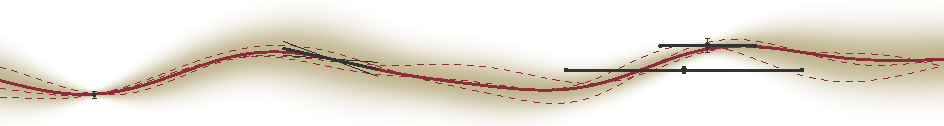
\includegraphics[width=0.9995\paperwidth]{\assetsDIR/logo_TU_169_1.pdf}};
  \end{tikzpicture}%
  }%
  %%%%%%%%%%%%%% END OF STATIC LOGO %%%%%%%%%%%%%

\end{frame}
\tikzexternalenable

\setlength{\figurewidth}{.9\textwidth}
\setlength{\figureheight}{.6\textheight}


%%%%%%%%%%%%%%%%
%   0 - Motivation and context
%%%%%%%%%%%%%%%%
\begin{frame}\frametitle{Motivation}
    \framesubtitle{Why do we need fast uncertainty in neural networks?}
    \begin{columns}
    	\column{0.55\textwidth}
		\begin{itemize}
			\item safety-critical applications e.g. self-driving cars
			\item trade-off between accuracy and speed
			\item out-of-distribution detection
		\end{itemize}
    	\column{0.45\textwidth}
    	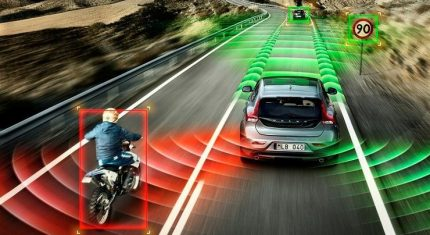
\includegraphics[width=\textwidth]{../figures/self-driving_car.jpg}
    \end{columns}
\end{frame}

%%%%%%%%%%%%%%%

\begin{frame}\frametitle{Context}
	\framesubtitle{What's our new contribution?}
	\begin{figure}
		\centering
		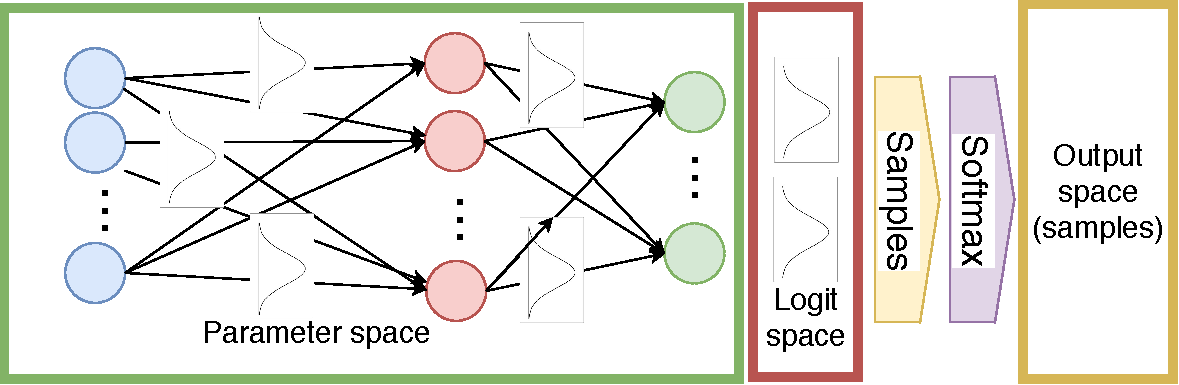
\includegraphics[height=0.4\textheight]{../figures/GaussNN_classic_slim.pdf}\\
		\vspace{4pt}
		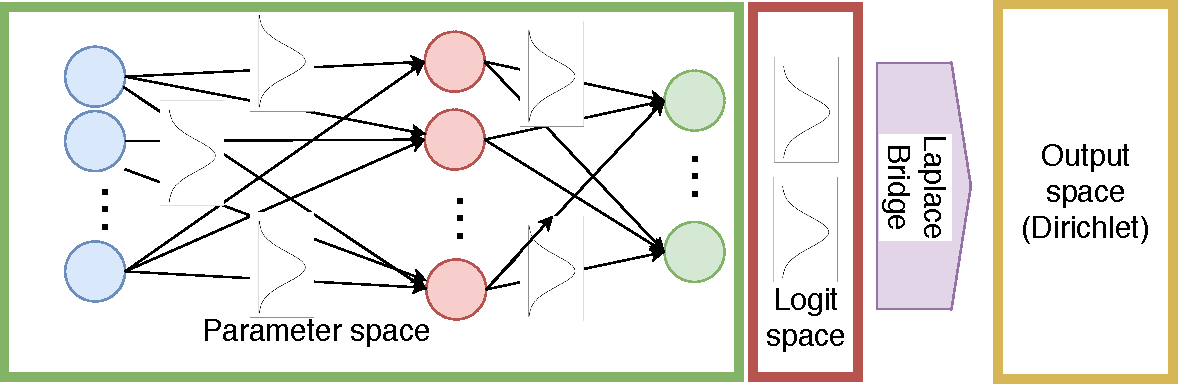
\includegraphics[height=0.4\textheight]{../figures/GaussNN_LaplaceBridge_slim.pdf}
	\end{figure}
\end{frame}


%%%%%%%%%%%%%%%%%%%%%%%%%
%     Theory
%%%%%%%%%%%%%%%%%%%%%%%%%
\blackslidetext{\center{\large\textbf{Theory}}}

\begin{frame}\frametitle{Background}
    \framesubtitle{Change of variable for PDFs}
	\subsection*{Change of Variable for pdf} 
	Let $\rvx$ be an $n$-dimensional continuous random variable with joint density function $p_\rvx$. If $\rvy = g(\rvx)$, where $g$ is a differentiable function, then $\rvy$ has density $p_\rvy$:
	\begin{equation}
	p_\rvy(\mathbf{y}) = p_\rvx\left(g^{-1}(\mathbf{\rvy})\right)\left\vert \det\left[\frac{dg^{-1}(\mathbf{\rvy})}{d\mathbf{\rvy}} \right]\right \vert
	\end{equation}
	where the differential is the Jacobian of the inverse of $g$ evaluated at $\rvy$. 
\end{frame}

%%%%%%%%%%%%%%%%%%%%%%%%%

\begin{frame}\frametitle{A new basis for the Dirichlet}
	\framesubtitle{The math}
	\begin{itemize}
		\item \begin{equation}\label{eq:dirichlet}
		\mathrm{Dir}(\vpi | \valpha) := \frac{1}{B(\alpha)}\prod_{k=1}^K \pi_k^{\alpha_k-1}
		\end{equation}
		\item \begin{equation}
		\pi_k(\vz) := \frac{\exp(z_k)}{\sum_{l=1}^K \exp(z_l)} \, ,
		\end{equation}
		\item \begin{equation}\label{eq:dirichlet_softmax}
		\mathrm{Dir}_{\vz}(\vpi(\vz) | \valpha) := \frac{1}{B(\alpha)}\prod_{k=1}^K \pi_k(\vz)^{\alpha_k} \, ,
		\end{equation}
	\end{itemize}
\end{frame}

%%%%%%%%%%%%%%%%%%%%%%%%%

\setlength{\figwidth}{0.5\textwidth}
\setlength{\figheight}{0.7\textheight}

\begin{frame}\frametitle{A new basis for the Dirichlet}
	\framesubtitle{In pictures}
	\begin{figure}
		\centering
		\scriptsize
		% This file was created by tikzplotlib v0.8.2.
\begin{tikzpicture}

\begin{groupplot}[group style={group size=2 by 1}]
\nextgroupplot[
height=\figheight,
legend cell align={left},
legend pos=north east,
legend style={draw=white!80.0!black},
tick align=outside,
tick pos=both,
title={Dirichlet in $\mathbb{P}$},
width=\figwidth,
x grid style={white!69.01960784313725!black},
xlabel={\(\displaystyle \pi\)},
xmin=-0.05, xmax=1.05,
xtick align=inside,
xtick pos=left,
xtick style={color=black},
xtick={-0.2,0,0.2,0.4,0.6,0.8,1,1.2},
xticklabels={−0.2,0.0,0.2,0.4,0.6,0.8,1.0,1.2},
ylabel={\(\displaystyle p(\pi)d\pi\)},
ymin=-0.158627690160108, ymax=3.33118149336226,
ytick align=inside,
ytick pos=left
]
\addplot [thick, red, opacity=1, forget plot]
table {%
0 inf
0.001 2.90783113913672
0.002 2.53166757054837
0.003 2.33470473994528
0.004 2.20438678938697
0.005 2.10838259723575
0.006 2.0330911190598
0.007 1.97156545015847
0.008 1.91980256320587
0.009 1.87529616056912
0.01 1.83637855436761
0.011 1.80188705642293
0.012 1.77098053614382
0.013 1.74303194282349
0.014 1.71756204006349
0.015 1.69419679932043
0.016 1.67263902561622
0.017 1.65264888800585
0.018 1.63403021179632
0.019 1.61662060862182
0.02 1.60028422849058
0.021 1.58490634357339
0.022 1.57038923729693
0.023 1.55664904024092
0.024 1.54361326384251
0.025 1.53121885586875
0.026 1.51941065117941
0.027 1.50814012556876
0.028 1.49736438455112
0.029 1.48704533612189
0.03 1.47714900893254
0.031 1.46764498639812
0.032 1.4585059339773
0.033 1.44970720189504
0.034 1.4412264893794
0.035 1.43304355938416
0.036 1.4251399950004
0.037 1.41749899049168
0.038 1.41010517124115
0.039 1.40294443796455
0.04 1.39600383138846
0.041 1.38927141426723
0.042 1.38273616815349
0.043 1.37638790277418
0.044 1.37021717621898
0.045 1.36421522443741
0.046 1.3583738987787
0.047 1.35268561050378
0.048 1.34714328136121
0.049 1.34174029945297
0.05 1.33647047972882
0.051 1.33132802854189
0.052 1.32630751177735
0.053 1.32140382613287
0.054 1.31661217318625
0.055 1.31192803593353
0.056 1.30734715752216
0.057 1.30286552193856
0.058 1.29847933643975
0.059 1.29418501554444
0.06 1.28997916642131
0.061 1.28585857553152
0.062 1.28182019639905
0.063 1.27786113839743
0.064 1.27397865645335
0.065 1.27017014157951
0.066 1.26643311215806
0.067 1.26276520590486
0.068 1.25916417245208
0.069 1.25562786649316
0.07 1.2521542414402
0.071 1.24874134354855
0.072 1.24538730646835
0.073 1.24209034618631
0.074 1.23884875632511
0.075 1.2356609037705
0.076 1.23252522459924
0.077 1.22944022028367
0.078 1.22640445415056
0.079 1.22341654807446
0.08 1.22047517938697
0.081 1.21757907798563
0.082 1.21472702362704
0.083 1.2119178433904
0.084 1.20915040929896
0.085 1.20642363608769
0.086 1.20373647910655
0.087 1.20108793234981
0.088 1.19847702660229
0.089 1.19590282769448
0.09 1.19336443485897
0.091 1.19086097918124
0.092 1.18839162213841
0.093 1.18595555422009
0.094 1.18355199362589
0.095 1.1811801850345
0.096 1.17883939843985
0.097 1.1765289280498
0.098 1.17424809124368
0.099 1.17199622758469
0.1 1.16977269788399
0.101 1.16757688331314
0.102 1.16540818456195
0.103 1.16326602103908
0.104 1.16114983011277
0.105 1.15905906638933
0.106 1.15699320102713
0.107 1.15495172108414
0.108 1.15293412889695
0.109 1.15093994148957
0.11 1.14896869001031
0.111 1.14701991919507
0.112 1.14509318685574
0.113 1.14318806339216
0.114 1.1413041313265
0.115 1.13944098485871
0.116 1.13759822944201
0.117 1.13577548137734
0.118 1.13397236742568
0.119 1.13218852443747
0.12 1.13042359899805
0.121 1.12867724708849
0.122 1.12694913376085
0.123 1.12523893282727
0.124 1.12354632656214
0.125 1.12187100541665
0.126 1.12021266774528
0.127 1.1185710195434
0.128 1.11694577419563
0.129 1.11533665223443
0.13 1.11374338110826
0.131 1.11216569495908
0.132 1.1106033344086
0.133 1.10905604635294
0.134 1.10752358376523
0.135 1.10600570550592
0.136 1.10450217614034
0.137 1.10301276576312
0.138 1.10153724982944
0.139 1.1000754089924
0.14 1.0986270289466
0.141 1.09719190027745
0.142 1.09576981831604
0.143 1.09436058299926
0.144 1.09296399873505
0.145 1.09157987427245
0.146 1.0902080225763
0.147 1.08884826070643
0.148 1.08750040970106
0.149 1.08616429446429
0.15 1.08483974365751
0.151 1.0835265895946
0.152 1.08222466814063
0.153 1.08093381861414
0.154 1.07965388369259
0.155 1.07838470932116
0.156 1.0771261446244
0.157 1.075878041821
0.158 1.07464025614128
0.159 1.07341264574736
0.16 1.07219507165603
0.161 1.07098739766402
0.162 1.06978949027576
0.163 1.06860121863338
0.164 1.06742245444895
0.165 1.06625307193896
0.166 1.06509294776068
0.167 1.06394196095067
0.168 1.06279999286511
0.169 1.061666927122
0.17 1.06054264954516
0.171 1.05942704810984
0.172 1.05832001289012
0.173 1.05722143600777
0.174 1.05613121158273
0.175 1.05504923568502
0.176 1.05397540628809
0.177 1.05290962322352
0.178 1.05185178813711
0.179 1.05080180444619
0.18 1.04975957729815
0.181 1.04872501353027
0.182 1.04769802163056
0.183 1.04667851169986
0.184 1.04566639541487
0.185 1.04466158599233
0.186 1.0436639981542
0.187 1.04267354809371
0.188 1.04169015344247
0.189 1.04071373323842
0.19 1.0397442078947
0.191 1.03878149916933
0.192 1.03782553013572
0.193 1.03687622515403
0.194 1.03593350984321
0.195 1.03499731105389
0.196 1.03406755684188
0.197 1.0331441764425
0.198 1.03222710024543
0.199 1.0313162597704
0.2 1.03041158764334
0.201 1.02951301757327
0.202 1.02862048432974
0.203 1.02773392372084
0.204 1.0268532725718
0.205 1.02597846870412
0.206 1.02510945091524
0.207 1.02424615895867
0.208 1.0233885335247
0.209 1.02253651622157
0.21 1.02169004955701
0.211 1.02084907692041
0.212 1.02001354256526
0.213 1.01918339159214
0.214 1.01835856993205
0.215 1.0175390243302
0.216 1.01672470233014
0.217 1.01591555225832
0.218 1.01511152320896
0.219 1.01431256502936
0.22 1.01351862830549
0.221 1.01272966434794
0.222 1.0119456251782
0.223 1.01116646351532
0.224 1.01039213276273
0.225 1.00962258699555
0.226 1.00885778094807
0.227 1.00809767000154
0.228 1.00734221017227
0.229 1.00659135809998
0.23 1.00584507103641
0.231 1.00510330683421
0.232 1.00436602393604
0.233 1.00363318136397
0.234 1.00290473870905
0.235 1.00218065612118
0.236 1.00146089429915
0.237 1.00074541448091
0.238 1.0000341784341
0.239 0.999327148446722
0.24 0.998624287318032
0.241 0.997925558349672
0.242 0.997230925336943
0.243 0.996540352560284
0.244 0.995853804776934
0.245 0.995171247212774
0.246 0.994492645554334
0.247 0.993817965940979
0.248 0.993147174957247
0.249 0.992480239625362
0.25 0.991817127397891
0.251 0.991157806150559
0.252 0.990502244175217
0.253 0.989850410172946
0.254 0.98920227324731
0.255 0.988557802897746
0.256 0.987916969013081
0.257 0.987279741865197
0.258 0.986646092102806
0.259 0.986015990745364
0.26 0.985389409177102
0.261 0.984766319141173
0.262 0.984146692733924
0.263 0.983530502399274
0.264 0.98291772092321
0.265 0.982308321428383
0.266 0.981702277368821
0.267 0.981099562524735
0.268 0.980500150997432
0.269 0.979904017204328
0.27 0.979311135874053
0.271 0.978721482041654
0.272 0.978135031043887
0.273 0.977551758514604
0.274 0.976971640380223
0.275 0.976394652855285
0.276 0.9758207724381
0.277 0.97524997590647
0.278 0.974682240313493
0.279 0.974117542983446
0.28 0.97355586150775
0.281 0.972997173741
0.282 0.97244145779708
0.283 0.971888692045339
0.284 0.971338855106847
0.285 0.970791925850712
0.286 0.970247883390472
0.287 0.969706707080545
0.288 0.969168376512747
0.289 0.968632871512878
0.29 0.968100172137359
0.291 0.96757025866994
0.292 0.967043111618459
0.293 0.966518711711667
0.294 0.9659970398961
0.295 0.965478077333014
0.296 0.964961805395375
0.297 0.964448205664893
0.298 0.963937259929117
0.299 0.963428950178582
0.3 0.962923258603993
0.301 0.962420167593478
0.302 0.961919659729869
0.303 0.961421717788044
0.304 0.960926324732306
0.305 0.960433463713817
0.306 0.959943118068061
0.307 0.959455271312368
0.308 0.958969907143466
0.309 0.958487009435084
0.31 0.958006562235587
0.311 0.957528549765661
0.312 0.957052956416028
0.313 0.956579766745205
0.314 0.956108965477298
0.315 0.955640537499834
0.316 0.955174467861626
0.317 0.954710741770682
0.318 0.954249344592136
0.319 0.953790261846223
0.32 0.953333479206285
0.321 0.952878982496806
0.322 0.952426757691486
0.323 0.951976790911339
0.324 0.951529068422824
0.325 0.951083576636014
0.326 0.950640302102782
0.327 0.950199231515026
0.328 0.949760351702919
0.329 0.949323649633185
0.33 0.948889112407407
0.331 0.948456727260359
0.332 0.948026481558367
0.333 0.947598362797691
0.334 0.947172358602941
0.335 0.946748456725507
0.336 0.946326645042025
0.337 0.945906911552861
0.338 0.945489244380617
0.339 0.945073631768666
0.34 0.944660062079703
0.341 0.94424852379433
0.342 0.943839005509647
0.343 0.943431495937877
0.344 0.943025983905009
0.345 0.94262245834946
0.346 0.942220908320761
0.347 0.941821322978258
0.348 0.941423691589837
0.349 0.941028003530669
0.35 0.940634248281969
0.351 0.940242415429784
0.352 0.939852494663783
0.353 0.939464475776083
0.354 0.939078348660083
0.355 0.938694103309312
0.356 0.938311729816307
0.357 0.937931218371498
0.358 0.937552559262106
0.359 0.937175742871073
0.36 0.936800759675992
0.361 0.936427600248062
0.362 0.936056255251053
0.363 0.935686715440293
0.364 0.935318971661662
0.365 0.93495301485061
0.366 0.934588836031178
0.367 0.934226426315045
0.368 0.93386577690058
0.369 0.933506879071914
0.37 0.933149724198023
0.371 0.932794303731822
0.372 0.932440609209277
0.373 0.932088632248528
0.374 0.931738364549019
0.375 0.931389797890655
0.376 0.931042924132953
0.377 0.930697735214219
0.378 0.930354223150732
0.379 0.930012380035937
0.38 0.929672198039656
0.381 0.929333669407304
0.382 0.928996786459118
0.383 0.928661541589405
0.384 0.928327927265782
0.385 0.927995936028449
0.386 0.927665560489457
0.387 0.927336793331991
0.388 0.927009627309664
0.389 0.926684055245821
0.39 0.926360070032854
0.391 0.926037664631519
0.392 0.925716832070275
0.393 0.925397565444624
0.394 0.925079857916458
0.395 0.924763702713426
0.396 0.9244490931283
0.397 0.924136022518351
0.398 0.923824484304741
0.399 0.923514471971914
0.4 0.923205979067002
0.401 0.922898999199239
0.402 0.922593526039375
0.403 0.922289553319116
0.404 0.921987074830548
0.405 0.92168608442559
0.406 0.921386576015444
0.407 0.921088543570053
0.408 0.920791981117572
0.409 0.920496882743838
0.41 0.920203242591857
0.411 0.919911054861292
0.412 0.919620313807957
0.413 0.919331013743323
0.414 0.919043149034028
0.415 0.918756714101394
0.416 0.91847170342095
0.417 0.918188111521963
0.418 0.917905932986979
0.419 0.91762516245136
0.42 0.917345794602836
0.421 0.917067824181066
0.422 0.916791245977193
0.423 0.916516054833418
0.424 0.916242245642572
0.425 0.915969813347696
0.426 0.915698752941631
0.427 0.915429059466605
0.428 0.915160728013834
0.429 0.914893753723123
0.43 0.91462813178248
0.431 0.914363857427723
0.432 0.914100925942106
0.433 0.913839332655943
0.434 0.913579072946235
0.435 0.913320142236313
0.436 0.913062535995468
0.437 0.91280624973861
0.438 0.912551279025906
0.439 0.912297619462447
0.44 0.912045266697902
0.441 0.911794216426184
0.442 0.911544464385126
0.443 0.91129600635615
0.444 0.911048838163949
0.445 0.910802955676173
0.446 0.910558354803114
0.447 0.910315031497405
0.448 0.910072981753714
0.449 0.909832201608446
0.45 0.909592687139453
0.451 0.909354434465741
0.452 0.90911743974719
0.453 0.908881699184266
0.454 0.908647209017755
0.455 0.90841396552848
0.456 0.908181965037039
0.457 0.907951203903539
0.458 0.907721678527338
0.459 0.907493385346784
0.46 0.907266320838965
0.461 0.907040481519463
0.462 0.906815863942103
0.463 0.906592464698718
0.464 0.906370280418908
0.465 0.906149307769807
0.466 0.905929543455855
0.467 0.905710984218568
0.468 0.905493626836318
0.469 0.905277468124113
0.47 0.905062504933381
0.471 0.904848734151756
0.472 0.904636152702873
0.473 0.904424757546159
0.474 0.904214545676632
0.475 0.904005514124703
0.476 0.90379765995598
0.477 0.903590980271074
0.478 0.903385472205415
0.479 0.90318113292906
0.48 0.902977959646515
0.481 0.902775949596555
0.482 0.902575100052045
0.483 0.902375408319771
0.484 0.902176871740267
0.485 0.901979487687649
0.486 0.901783253569453
0.487 0.901588166826469
0.488 0.901394224932589
0.489 0.901201425394649
0.49 0.901009765752278
0.491 0.900819243577748
0.492 0.900629856475829
0.493 0.900441602083644
0.494 0.900254478070532
0.495 0.900068482137906
0.496 0.899883612019124
0.497 0.899699865479348
0.498 0.899517240315428
0.499 0.899335734355762
0.5 0.899155345460183
0.501 0.898976071519832
0.502 0.898797910457041
0.503 0.898620860225221
0.504 0.898444918808743
0.505 0.898270084222836
0.506 0.898096354513471
0.507 0.897923727757264
0.508 0.897752202061368
0.509 0.897581775563376
0.51 0.897412446431227
0.511 0.897244212863104
0.512 0.897077073087351
0.513 0.896911025362378
0.514 0.896746067976577
0.515 0.896582199248238
0.516 0.896419417525466
0.517 0.896257721186103
0.518 0.896097108637653
0.519 0.895937578317205
0.52 0.895779128691366
0.521 0.895621758256188
0.522 0.895465465537102
0.523 0.895310249088858
0.524 0.89515610749546
0.525 0.895003039370107
0.526 0.89485104335514
0.527 0.894700118121984
0.528 0.894550262371099
0.529 0.89440147483193
0.53 0.894253754262861
0.531 0.894107099451171
0.532 0.893961509212989
0.533 0.893816982393261
0.534 0.893673517865709
0.535 0.893531114532797
0.536 0.8933897713257
0.537 0.893249487204274
0.538 0.893110261157029
0.539 0.892972092201104
0.54 0.892834979382248
0.541 0.892698921774796
0.542 0.892563918481653
0.543 0.892429968634281
0.544 0.892297071392686
0.545 0.892165225945406
0.546 0.892034431509507
0.547 0.891904687330575
0.548 0.891775992682716
0.549 0.891648346868555
0.55 0.891521749219235
0.551 0.891396199094431
0.552 0.891271695882347
0.553 0.891148238999733
0.554 0.891025827891894
0.555 0.890904462032707
0.556 0.890784140924636
0.557 0.890664864098756
0.558 0.890546631114771
0.559 0.890429441561041
0.56 0.890313295054612
0.561 0.890198191241242
0.562 0.890084129795436
0.563 0.889971110420481
0.564 0.889859132848484
0.565 0.889748196840415
0.566 0.889638302186143
0.567 0.889529448704491
0.568 0.889421636243278
0.569 0.889314864679372
0.57 0.889209133918747
0.571 0.889104443896531
0.572 0.889000794577076
0.573 0.888898185954013
0.574 0.888796618050318
0.575 0.888696090918381
0.576 0.888596604640073
0.577 0.888498159326824
0.578 0.888400755119695
0.579 0.888304392189457
0.58 0.888209070736676
0.581 0.888114790991792
0.582 0.88802155321521
0.583 0.887929357697391
0.584 0.887838204758943
0.585 0.887748094750718
0.586 0.887659028053911
0.587 0.887571005080162
0.588 0.887484026271662
0.589 0.887398092101264
0.59 0.887313203072587
0.591 0.887229359720138
0.592 0.887146562609427
0.593 0.887064812337086
0.594 0.886984109530997
0.595 0.886904454850417
0.596 0.886825848986109
0.597 0.886748292660476
0.598 0.886671786627698
0.599 0.886596331673874
0.6 0.886521928617166
0.601 0.886448578307945
0.602 0.886376281628943
0.603 0.886305039495409
0.604 0.886234852855263
0.605 0.886165722689265
0.606 0.886097650011172
0.607 0.886030635867913
0.608 0.885964681339759
0.609 0.885899787540501
0.61 0.885835955617631
0.611 0.885773186752523
0.612 0.885711482160625
0.613 0.885650843091647
0.614 0.885591270829762
0.615 0.885532766693802
0.616 0.885475332037464
0.617 0.885418968249519
0.618 0.885363676754022
0.619 0.88530945901053
0.62 0.885256316514325
0.621 0.885204250796639
0.622 0.885153263424878
0.623 0.885103356002866
0.624 0.885054530171077
0.625 0.885006787606879
0.626 0.884960130024785
0.627 0.884914559176705
0.628 0.8848700768522
0.629 0.88482668487875
0.63 0.884784385122017
0.631 0.884743179486119
0.632 0.884703069913908
0.633 0.884664058387251
0.634 0.884626146927319
0.635 0.884589337594878
0.636 0.884553632490591
0.637 0.884519033755317
0.638 0.884485543570423
0.639 0.884453164158101
0.64 0.884421897781681
0.641 0.884391746745966
0.642 0.884362713397559
0.643 0.884334800125202
0.644 0.884308009360119
0.645 0.884282343576369
0.646 0.884257805291199
0.647 0.884234397065408
0.648 0.884212121503717
0.649 0.884190981255143
0.65 0.884170979013382
0.651 0.884152117517197
0.652 0.884134399550813
0.653 0.884117827944323
0.654 0.884102405574092
0.655 0.884088135363179
0.656 0.884075020281758
0.657 0.884063063347551
0.658 0.884052267626263
0.659 0.884042636232035
0.66 0.884034172327892
0.661 0.884026879126208
0.662 0.884020759889177
0.663 0.884015817929289
0.664 0.884012056609817
0.665 0.884009479345313
0.666 0.884008089602113
0.667 0.884007890898844
0.668 0.884008886806952
0.669 0.884011080951226
0.67 0.884014477010341
0.671 0.884019078717406
0.672 0.884024889860521
0.673 0.884031914283347
0.674 0.884040155885684
0.675 0.884049618624054
0.676 0.884060306512305
0.677 0.884072223622215
0.678 0.884085374084114
0.679 0.884099762087513
0.68 0.884115391881743
0.681 0.884132267776608
0.682 0.884150394143049
0.683 0.884169775413818
0.684 0.884190416084165
0.685 0.884212320712536
0.686 0.884235493921284
0.687 0.884259940397394
0.688 0.884285664893218
0.689 0.884312672227221
0.69 0.88434096728475
0.691 0.884370555018804
0.692 0.884401440450824
0.693 0.884433628671503
0.694 0.884467124841592
0.695 0.884501934192743
0.696 0.884538062028351
0.697 0.884575513724414
0.698 0.884614294730418
0.699 0.884654410570222
0.7 0.884695866842972
0.701 0.884738669224027
0.702 0.884782823465896
0.703 0.884828335399204
0.704 0.884875210933664
0.705 0.884923456059075
0.706 0.884973076846329
0.707 0.885024079448446
0.708 0.885076470101624
0.709 0.885130255126306
0.71 0.885185440928265
0.711 0.885242033999721
0.712 0.88530004092046
0.713 0.885359468358993
0.714 0.885420323073717
0.715 0.885482611914116
0.716 0.885546341821972
0.717 0.885611519832602
0.718 0.885678153076119
0.719 0.885746248778718
0.72 0.88581581426398
0.721 0.885886856954212
0.722 0.885959384371796
0.723 0.886033404140583
0.724 0.886108923987293
0.725 0.886185951742961
0.726 0.886264495344397
0.727 0.886344562835677
0.728 0.88642616236967
0.729 0.886509302209585
0.73 0.886593990730549
0.731 0.886680236421226
0.732 0.886768047885454
0.733 0.886857433843919
0.734 0.886948403135868
0.735 0.887040964720847
0.736 0.887135127680474
0.737 0.887230901220256
0.738 0.88732829467143
0.739 0.887427317492849
0.74 0.887527979272901
0.741 0.887630289731474
0.742 0.887734258721946
0.743 0.887839896233233
0.744 0.887947212391863
0.745 0.888056217464103
0.746 0.888166921858124
0.747 0.888279336126209
0.748 0.888393470967013
0.749 0.888509337227862
0.75 0.888626945907103
0.751 0.888746308156506
0.752 0.88886743528371
0.753 0.88899033875472
0.754 0.889115030196467
0.755 0.889241521399406
0.756 0.889369824320183
0.757 0.889499951084348
0.758 0.889631913989135
0.759 0.889765725506294
0.76 0.889901398284987
0.761 0.890038945154746
0.762 0.890178379128496
0.763 0.890319713405644
0.764 0.890462961375231
0.765 0.890608136619157
0.766 0.890755252915478
0.767 0.890904324241771
0.768 0.891055364778579
0.769 0.891208388912929
0.77 0.891363411241926
0.771 0.891520446576437
0.772 0.89167950994485
0.773 0.891840616596917
0.774 0.892003782007692
0.775 0.89216902188155
0.776 0.892336352156308
0.777 0.892505789007428
0.778 0.892677348852329
0.779 0.892851048354794
0.78 0.893026904429478
0.781 0.893204934246524
0.782 0.893385155236288
0.783 0.893567585094174
0.784 0.893752241785584
0.785 0.893939143550986
0.786 0.894128308911103
0.787 0.89431975667223
0.788 0.894513505931672
0.789 0.894709576083323
0.79 0.894907986823373
0.791 0.895108758156161
0.792 0.895311910400166
0.793 0.895517464194152
0.794 0.895725440503463
0.795 0.895935860626473
0.796 0.8961487462012
0.797 0.896364119212089
0.798 0.89658200199696
0.799 0.896802417254138
0.8 0.897025388049764
0.801 0.897250937825297
0.802 0.897479090405198
0.803 0.897709870004831
0.804 0.897943301238555
0.805 0.898179409128034
0.806 0.898418219110766
0.807 0.898659757048837
0.808 0.898904049237909
0.809 0.899151122416447
0.81 0.899401003775192
0.811 0.899653720966894
0.812 0.899909302116308
0.813 0.90016777583046
0.814 0.900429171209201
0.815 0.900693517856045
0.816 0.90096084588931
0.817 0.901231185953576
0.818 0.901504569231453
0.819 0.901781027455688
0.82 0.902060592921618
0.821 0.902343298499968
0.822 0.902629177650024
0.823 0.902918264433185
0.824 0.903210593526902
0.825 0.903506200239032
0.826 0.903805120522602
0.827 0.904107390991019
0.828 0.904413048933725
0.829 0.904722132332318
0.83 0.905034679877161
0.831 0.905350730984487
0.832 0.905670325814029
0.833 0.905993505287179
0.834 0.906320311105718
0.835 0.90665078577111
0.836 0.906984972604406
0.837 0.907322915766769
0.838 0.907664660280637
0.839 0.908010252051568
0.84 0.90835973789077
0.841 0.908713165538358
0.842 0.909070583687364
0.843 0.909432042008517
0.844 0.909797591175843
0.845 0.9101672828931
0.846 0.910541169921085
0.847 0.910919306105861
0.848 0.911301746407919
0.849 0.911688546932327
0.85 0.912079764959905
0.851 0.912475458979466
0.852 0.912875688721162
0.853 0.913280515190988
0.854 0.913690000706491
0.855 0.914104208933732
0.856 0.914523204925553
0.857 0.914947055161207
0.858 0.915375827587415
0.859 0.915809591660895
0.86 0.916248418392449
0.861 0.916692380392654
0.862 0.917141551919247
0.863 0.917596008926265
0.864 0.91805582911503
0.865 0.918521091987049
0.866 0.918991878898928
0.867 0.919468273119391
0.868 0.919950359888487
0.869 0.920438226479108
0.87 0.920931962260908
0.871 0.921431658766749
0.872 0.921937409761782
0.873 0.922449311315302
0.874 0.922967461875501
0.875 0.923491962347265
0.876 0.924022916173163
0.877 0.924560429417787
0.878 0.925104610855603
0.879 0.925655572062507
0.88 0.926213427511249
0.881 0.926778294670944
0.882 0.927350294110871
0.883 0.927929549608786
0.884 0.928516188263974
0.885 0.929110340615316
0.886 0.929712140764612
0.887 0.930321726505454
0.888 0.930939239457959
0.889 0.931564825209663
0.89 0.932198633462932
0.891 0.932840818189252
0.892 0.933491537790778
0.893 0.93415095526956
0.894 0.934819238404883
0.895 0.935496559939197
0.896 0.936183097773127
0.897 0.936879035170113
0.898 0.937584560971244
0.899 0.938299869820903
0.9 0.939025162403876
0.901 0.939760645694634
0.902 0.940506533219546
0.903 0.941263045332815
0.904 0.942030409507031
0.905 0.942808860639251
0.906 0.94359864137363
0.907 0.944400002441672
0.908 0.945213203021261
0.909 0.946038511115747
0.91 0.946876203954404
0.911 0.947726568415761
0.912 0.948589901475348
0.913 0.949466510679579
0.914 0.950356714647618
0.915 0.951260843603219
0.916 0.952179239938711
0.917 0.953112258813483
0.918 0.954060268789506
0.919 0.955023652506696
0.92 0.956002807401108
0.921 0.956998146469279
0.922 0.958010099082297
0.923 0.959039111853506
0.924 0.960085649564156
0.925 0.961150196151653
0.926 0.962233255765568
0.927 0.963335353897019
0.928 0.964457038587606
0.929 0.965598881724718
0.93 0.966761480430652
0.931 0.967945458553838
0.932 0.969151468271231
0.933 0.970380191811952
0.934 0.971632343313318
0.935 0.972908670821583
0.936 0.974209958451117
0.937 0.975537028717256
0.938 0.976890745059783
0.939 0.978272014575994
0.94 0.979681790984494
0.941 0.981121077843414
0.942 0.982590932049618
0.943 0.984092467648743
0.944 0.985626859989688
0.945 0.987195350261449
0.946 0.98879925045518
0.947 0.9904399488
0.948 0.992118915727709
0.949 0.99383771042912
0.95 0.995597988073604
0.951 0.997401507773681
0.952 0.999250141388526
0.953 1.00114588327428
0.954 1.00309086110561
0.955 1.00508734791225
0.956 1.00713777549757
0.957 1.00924474943306
0.958 1.01141106585544
0.959 1.01363973033187
0.96 1.01593397910517
0.961 1.01829730308743
0.962 1.02073347503815
0.963 1.02324658044601
0.964 1.02584105273453
0.965 1.02852171353591
0.966 1.03129381893124
0.967 1.03416311274576
0.968 1.03713588822622
0.969 1.04021905972748
0.97 1.04342024641469
0.971 1.04674787047195
0.972 1.05021127293016
0.973 1.05382085103273
0.974 1.05758822211064
0.975 1.06152642032651
0.976 1.0656501344962
0.977 1.06997599768436
0.978 1.07452294265708
0.979 1.07931264194234
0.98 1.08437005776789
0.981 1.08972413638411
0.982 1.09540869458031
0.983 1.10146356568972
0.984 1.10793610148096
0.985 1.11488317073044
0.986 1.12237386461961
0.987 1.13049323034237
0.988 1.13934753817339
0.989 1.14907190170824
0.99 1.15984163033886
0.991 1.17188973451849
0.992 1.18553505101674
0.993 1.20122974605795
0.994 1.21964469155695
0.995 1.24183562716843
0.996 1.26960278080034
0.997 1.30639519587921
0.998 1.36018074932806
0.999 1.457513661475
1 inf
};
\addplot [thick, blue, opacity=1, forget plot]
table {%
0 0
0.001 1.998e-08
0.002 1.5968e-07
0.003 5.3838e-07
0.004 1.27488e-06
0.005 2.4875e-06
0.006 4.29408e-06
0.007 6.81198e-06
0.008 1.015808e-05
0.009 1.444878e-05
0.01 1.98e-05
0.011 2.632718e-05
0.012 3.414528e-05
0.013 4.336878e-05
0.014 5.411168e-05
0.015 6.64875e-05
0.016 8.060928e-05
0.017 9.658958e-05
0.018 0.00011454048
0.019 0.00013457358
0.02 0.0001568
0.021 0.00018133038
0.022 0.00020827488
0.023 0.00023774318
0.024 0.00026984448
0.025 0.0003046875
0.026 0.00034238048
0.027 0.00038303118
0.028 0.00042674688
0.029 0.00047363438
0.03 0.0005238
0.031 0.00057734958
0.032 0.00063438848
0.033 0.00069502158
0.034 0.00075935328
0.035 0.0008274875
0.036 0.00089952768
0.037 0.00097557678
0.038 0.00105573728
0.039 0.00114011118
0.04 0.0012288
0.041 0.00132190478
0.042 0.00141952608
0.043 0.00152176398
0.044 0.00162871808
0.045 0.0017404875
0.046 0.00185717088
0.047 0.00197886638
0.048 0.00210567168
0.049 0.00223768398
0.05 0.002375
0.051 0.00251771598
0.052 0.00266592768
0.053 0.00281973038
0.054 0.00297921888
0.055 0.0031444875
0.056 0.00331563008
0.057 0.00349273998
0.058 0.00367591008
0.059 0.00386523278
0.06 0.0040608
0.061 0.00426270318
0.062 0.00447103328
0.063 0.00468588078
0.064 0.00490733568
0.065 0.0051354875
0.066 0.00537042528
0.067 0.00561223758
0.068 0.00586101248
0.069 0.00611683758
0.07 0.0063798
0.071 0.00664998638
0.072 0.00692748288
0.073 0.00721237518
0.074 0.00750474848
0.075 0.0078046875
0.076 0.00811227648
0.077 0.00842759918
0.078 0.00875073888
0.079 0.00908177838
0.08 0.0094208
0.081 0.00976788558
0.082 0.01012311648
0.083 0.01048657358
0.084 0.01085833728
0.085 0.0112384875
0.086 0.01162710368
0.087 0.01202426478
0.088 0.01243004928
0.089 0.01284453518
0.09 0.0132678
0.091 0.01369992078
0.092 0.01414097408
0.093 0.01459103598
0.094 0.01505018208
0.095 0.0155184875
0.096 0.01599602688
0.097 0.01648287438
0.098 0.01697910368
0.099 0.01748478798
0.1 0.018
0.101 0.01852481198
0.102 0.01905929568
0.103 0.01960352238
0.104 0.02015756288
0.105 0.0207214875
0.106 0.02129536608
0.107 0.02187926798
0.108 0.02247326208
0.109 0.02307741678
0.11 0.0236918
0.111 0.02431647918
0.112 0.02495152128
0.113 0.02559699278
0.114 0.02625295968
0.115 0.0269194875
0.116 0.02759664128
0.117 0.02828448558
0.118 0.02898308448
0.119 0.02969250158
0.12 0.0304128
0.121 0.03114404238
0.122 0.03188629088
0.123 0.03263960718
0.124 0.03340405248
0.125 0.0341796875
0.126 0.03496657248
0.127 0.03576476718
0.128 0.03657433088
0.129 0.03739532238
0.13 0.0382278
0.131 0.03907182158
0.132 0.03992744448
0.133 0.04079472558
0.134 0.04167372128
0.135 0.0425644875
0.136 0.04346707968
0.137 0.04438155278
0.138 0.04530796128
0.139 0.04624635918
0.14 0.0471968
0.141 0.04815933678
0.142 0.04913402208
0.143 0.05012090798
0.144 0.05112004608
0.145 0.0521314875
0.146 0.05315528288
0.147 0.05419148238
0.148 0.05524013568
0.149 0.05630129198
0.15 0.057375
0.151 0.05846130798
0.152 0.05956026368
0.153 0.06067191438
0.154 0.06179630688
0.155 0.0629334875
0.156 0.06408350208
0.157 0.06524639598
0.158 0.06642221408
0.159 0.06761100078
0.16 0.0688128
0.161 0.07002765518
0.162 0.07125560928
0.163 0.07249670478
0.164 0.07375098368
0.165 0.0750184875
0.166 0.07629925728
0.167 0.07759333358
0.168 0.07890075648
0.169 0.08022156558
0.17 0.0815558
0.171 0.08290349838
0.172 0.08426469888
0.173 0.08563943918
0.174 0.08702775648
0.175 0.0884296875
0.176 0.08984526848
0.177 0.09127453518
0.178 0.09271752288
0.179 0.09417426638
0.18 0.0956448
0.181 0.09712915758
0.182 0.09862737248
0.183 0.10013947758
0.184 0.10166550528
0.185 0.1032054875
0.186 0.10475945568
0.187 0.10632744078
0.188 0.10790947328
0.189 0.10950558318
0.19 0.1111158
0.191 0.11274015278
0.192 0.11437867008
0.193 0.11603137998
0.194 0.11769831008
0.195 0.1193794875
0.196 0.12107493888
0.197 0.12278469038
0.198 0.12450876768
0.199 0.12624719598
0.2 0.128
0.201 0.12976720398
0.202 0.13154883168
0.203 0.13334490638
0.204 0.13515545088
0.205 0.1369804875
0.206 0.13882003808
0.207 0.14067412398
0.208 0.14254276608
0.209 0.14442598478
0.21 0.1463238
0.211 0.14823623118
0.212 0.15016329728
0.213 0.15210501678
0.214 0.15406140768
0.215 0.1560324875
0.216 0.15801827328
0.217 0.16001878158
0.218 0.16203402848
0.219 0.16406402958
0.22 0.1661088
0.221 0.16816835438
0.222 0.17024270688
0.223 0.17233187118
0.224 0.17443586048
0.225 0.1765546875
0.226 0.17868836448
0.227 0.18083690318
0.228 0.18300031488
0.229 0.18517861038
0.23 0.1873718
0.231 0.18957989358
0.232 0.19180290048
0.233 0.19404082958
0.234 0.19629368928
0.235 0.1985614875
0.236 0.20084423168
0.237 0.20314192878
0.238 0.20545458528
0.239 0.20778220718
0.24 0.2101248
0.241 0.21248236878
0.242 0.21485491808
0.243 0.21724245198
0.244 0.21964497408
0.245 0.2220624875
0.246 0.22449499488
0.247 0.22694249838
0.248 0.22940499968
0.249 0.23188249998
0.25 0.234375
0.251 0.23688249998
0.252 0.23940499968
0.253 0.24194249838
0.254 0.24449499488
0.255 0.2470624875
0.256 0.24964497408
0.257 0.25224245198
0.258 0.25485491808
0.259 0.25748236878
0.26 0.2601248
0.261 0.26278220718
0.262 0.26545458528
0.263 0.26814192878
0.264 0.27084423168
0.265 0.2735614875
0.266 0.27629368928
0.267 0.27904082958
0.268 0.28180290048
0.269 0.28457989358
0.27 0.2873718
0.271 0.29017861038
0.272 0.29300031488
0.273 0.29583690318
0.274 0.29868836448
0.275 0.3015546875
0.276 0.30443586048
0.277 0.30733187118
0.278 0.31024270688
0.279 0.31316835438
0.28 0.3161088
0.281 0.31906402958
0.282 0.32203402848
0.283 0.32501878158
0.284 0.32801827328
0.285 0.3310324875
0.286 0.33406140768
0.287 0.33710501678
0.288 0.34016329728
0.289 0.34323623118
0.29 0.3463238
0.291 0.34942598478
0.292 0.35254276608
0.293 0.35567412398
0.294 0.35882003808
0.295 0.3619804875
0.296 0.36515545088
0.297 0.36834490638
0.298 0.37154883168
0.299 0.37476720398
0.3 0.378
0.301 0.38124719598
0.302 0.38450876768
0.303 0.38778469038
0.304 0.39107493888
0.305 0.3943794875
0.306 0.39769831008
0.307 0.40103137998
0.308 0.40437867008
0.309 0.40774015278
0.31 0.4111158
0.311 0.41450558318
0.312 0.41790947328
0.313 0.42132744078
0.314 0.42475945568
0.315 0.4282054875
0.316 0.43166550528
0.317 0.43513947758
0.318 0.43862737248
0.319 0.44212915758
0.32 0.4456448
0.321 0.44917426638
0.322 0.45271752288
0.323 0.45627453518
0.324 0.45984526848
0.325 0.4634296875
0.326 0.46702775648
0.327 0.47063943918
0.328 0.47426469888
0.329 0.47790349838
0.33 0.4815558
0.331 0.48522156558
0.332 0.48890075648
0.333 0.49259333358
0.334 0.49629925728
0.335 0.5000184875
0.336 0.50375098368
0.337 0.50749670478
0.338 0.51125560928
0.339 0.51502765518
0.34 0.5188128
0.341 0.52261100078
0.342 0.52642221408
0.343 0.53024639598
0.344 0.53408350208
0.345 0.5379334875
0.346 0.54179630688
0.347 0.54567191438
0.348 0.54956026368
0.349 0.55346130798
0.35 0.557375
0.351 0.56130129198
0.352 0.56524013568
0.353 0.56919148238
0.354 0.57315528288
0.355 0.5771314875
0.356 0.58112004608
0.357 0.58512090798
0.358 0.58913402208
0.359 0.59315933678
0.36 0.5971968
0.361 0.60124635918
0.362 0.60530796128
0.363 0.60938155278
0.364 0.61346707968
0.365 0.6175644875
0.366 0.62167372128
0.367 0.62579472558
0.368 0.62992744448
0.369 0.63407182158
0.37 0.6382278
0.371 0.64239532238
0.372 0.64657433088
0.373 0.65076476718
0.374 0.65496657248
0.375 0.6591796875
0.376 0.66340405248
0.377 0.66763960718
0.378 0.67188629088
0.379 0.67614404238
0.38 0.6804128
0.381 0.68469250158
0.382 0.68898308448
0.383 0.69328448558
0.384 0.69759664128
0.385 0.7019194875
0.386 0.70625295968
0.387 0.71059699278
0.388 0.71495152128
0.389 0.71931647918
0.39 0.7236918
0.391 0.72807741678
0.392 0.73247326208
0.393 0.73687926798
0.394 0.74129536608
0.395 0.7457214875
0.396 0.75015756288
0.397 0.75460352238
0.398 0.75905929568
0.399 0.76352481198
0.4 0.768
0.401 0.77248478798
0.402 0.77697910368
0.403 0.78148287438
0.404 0.78599602688
0.405 0.7905184875
0.406 0.79505018208
0.407 0.79959103598
0.408 0.80414097408
0.409 0.80869992078
0.41 0.8132678
0.411 0.81784453518
0.412 0.82243004928
0.413 0.82702426478
0.414 0.83162710368
0.415 0.8362384875
0.416 0.84085833728
0.417 0.84548657358
0.418 0.85012311648
0.419 0.85476788558
0.42 0.8594208
0.421 0.86408177838
0.422 0.86875073888
0.423 0.87342759918
0.424 0.87811227648
0.425 0.8828046875
0.426 0.88750474848
0.427 0.89221237518
0.428 0.89692748288
0.429 0.90164998638
0.43 0.9063798
0.431 0.91111683758
0.432 0.91586101248
0.433 0.92061223758
0.434 0.92537042528
0.435 0.9301354875
0.436 0.93490733568
0.437 0.93968588078
0.438 0.94447103328
0.439 0.94926270318
0.44 0.9540608
0.441 0.95886523278
0.442 0.96367591008
0.443 0.96849273998
0.444 0.97331563008
0.445 0.9781444875
0.446 0.98297921888
0.447 0.98781973038
0.448 0.99266592768
0.449 0.99751771598
0.45 1.002375
0.451 1.00723768398
0.452 1.01210567168
0.453 1.01697886638
0.454 1.02185717088
0.455 1.0267404875
0.456 1.03162871808
0.457 1.03652176398
0.458 1.04141952608
0.459 1.04632190478
0.46 1.0512288
0.461 1.05614011118
0.462 1.06105573728
0.463 1.06597557678
0.464 1.07089952768
0.465 1.0758274875
0.466 1.08075935328
0.467 1.08569502158
0.468 1.09063438848
0.469 1.09557734958
0.47 1.1005238
0.471 1.10547363438
0.472 1.11042674688
0.473 1.11538303118
0.474 1.12034238048
0.475 1.1253046875
0.476 1.13026984448
0.477 1.13523774318
0.478 1.14020827488
0.479 1.14518133038
0.48 1.1501568
0.481 1.15513457358
0.482 1.16011454048
0.483 1.16509658958
0.484 1.17008060928
0.485 1.1750664875
0.486 1.18005411168
0.487 1.18504336878
0.488 1.19003414528
0.489 1.19502632718
0.49 1.2000198
0.491 1.20501444878
0.492 1.21001015808
0.493 1.21500681198
0.494 1.22000429408
0.495 1.2250024875
0.496 1.23000127488
0.497 1.23500053838
0.498 1.24000015968
0.499 1.24500001998
0.5 1.25
0.501 1.25499997998
0.502 1.25999983968
0.503 1.26499945838
0.504 1.26999871488
0.505 1.2749974875
0.506 1.27999565408
0.507 1.28499309198
0.508 1.28998967808
0.509 1.29498528878
0.51 1.2999798
0.511 1.30497308718
0.512 1.30996502528
0.513 1.31495548878
0.514 1.31994435168
0.515 1.3249314875
0.516 1.32991676928
0.517 1.33490006958
0.518 1.33988126048
0.519 1.34486021358
0.52 1.3498368
0.521 1.35481089038
0.522 1.35978235488
0.523 1.36475106318
0.524 1.36971688448
0.525 1.3746796875
0.526 1.37963934048
0.527 1.38459571118
0.528 1.38954866688
0.529 1.39449807438
0.53 1.3994438
0.531 1.40438570958
0.532 1.40932366848
0.533 1.41425754158
0.534 1.41918719328
0.535 1.4241124875
0.536 1.42903328768
0.537 1.43394945678
0.538 1.43886085728
0.539 1.44376735118
0.54 1.4486688
0.541 1.45356506478
0.542 1.45845600608
0.543 1.46334148398
0.544 1.46822135808
0.545 1.4730954875
0.546 1.47796373088
0.547 1.48282594638
0.548 1.48768199168
0.549 1.49253172398
0.55 1.497375
0.551 1.50221167598
0.552 1.50704160768
0.553 1.51186465038
0.554 1.51668065888
0.555 1.5214894875
0.556 1.52629099008
0.557 1.53108501998
0.558 1.53587143008
0.559 1.54065007278
0.56 1.5454208
0.561 1.55018346318
0.562 1.55493791328
0.563 1.55968400078
0.564 1.56442157568
0.565 1.5691504875
0.566 1.57387058528
0.567 1.57858171758
0.568 1.58328373248
0.569 1.58797647758
0.57 1.5926598
0.571 1.59733354638
0.572 1.60199756288
0.573 1.60665169518
0.574 1.61129578848
0.575 1.6159296875
0.576 1.62055323648
0.577 1.62516627918
0.578 1.62976865888
0.579 1.63436021838
0.58 1.6389408
0.581 1.64351024558
0.582 1.64806839648
0.583 1.65261509358
0.584 1.65715017728
0.585 1.6616734875
0.586 1.66618486368
0.587 1.67068414478
0.588 1.67517116928
0.589 1.67964577518
0.59 1.6841078
0.591 1.68855708078
0.592 1.69299345408
0.593 1.69741675598
0.594 1.70182682208
0.595 1.7062234875
0.596 1.71060658688
0.597 1.71497595438
0.598 1.71933142368
0.599 1.72367282798
0.6 1.728
0.601 1.73231277198
0.602 1.73661097568
0.603 1.74089444238
0.604 1.74516300288
0.605 1.7494164875
0.606 1.75365472608
0.607 1.75787754798
0.608 1.76208478208
0.609 1.76627625678
0.61 1.7704518
0.611 1.77461123918
0.612 1.77875440128
0.613 1.78288111278
0.614 1.78699119968
0.615 1.7910844875
0.616 1.79516080128
0.617 1.79921996558
0.618 1.80326180448
0.619 1.80728614158
0.62 1.8112928
0.621 1.81528160238
0.622 1.81925237088
0.623 1.82320492718
0.624 1.82713909248
0.625 1.8310546875
0.626 1.83495153248
0.627 1.83882944718
0.628 1.84268825088
0.629 1.84652776238
0.63 1.8503478
0.631 1.85414818158
0.632 1.85792872448
0.633 1.86168924558
0.634 1.86542956128
0.635 1.8691494875
0.636 1.87284883968
0.637 1.87652743278
0.638 1.88018508128
0.639 1.88382159918
0.64 1.8874368
0.641 1.89103049678
0.642 1.89460250208
0.643 1.89815262798
0.644 1.90168068608
0.645 1.9051864875
0.646 1.90866984288
0.647 1.91213056238
0.648 1.91556845568
0.649 1.91898333198
0.65 1.922375
0.651 1.92574326798
0.652 1.92908794368
0.653 1.93240883438
0.654 1.93570574688
0.655 1.9389784875
0.656 1.94222686208
0.657 1.94545067598
0.658 1.94864973408
0.659 1.95182384078
0.66 1.9549728
0.661 1.95809641518
0.662 1.96119448928
0.663 1.96426682478
0.664 1.96731322368
0.665 1.9703334875
0.666 1.97332741728
0.667 1.97629481358
0.668 1.97923547648
0.669 1.98214920558
0.67 1.9850358
0.671 1.98789505838
0.672 1.99072677888
0.673 1.99353075918
0.674 1.99630679648
0.675 1.9990546875
0.676 2.00177422848
0.677 2.00446521518
0.678 2.00712744288
0.679 2.00976070638
0.68 2.0123648
0.681 2.01493951758
0.682 2.01748465248
0.683 2.01999999758
0.684 2.02248534528
0.685 2.0249404875
0.686 2.02736521568
0.687 2.02975932078
0.688 2.03212259328
0.689 2.03445482318
0.69 2.0367558
0.691 2.03902531278
0.692 2.04126315008
0.693 2.04346909998
0.694 2.04564295008
0.695 2.0477844875
0.696 2.04989349888
0.697 2.05196977038
0.698 2.05401308768
0.699 2.05602323598
0.7 2.058
0.701 2.05994316398
0.702 2.06185251168
0.703 2.06372782638
0.704 2.06556889088
0.705 2.0673754875
0.706 2.06914739808
0.707 2.07088440398
0.708 2.07258628608
0.709 2.07425282478
0.71 2.0758838
0.711 2.07747899118
0.712 2.07903817728
0.713 2.08056113678
0.714 2.08204764768
0.715 2.0834974875
0.716 2.08491043328
0.717 2.08628626158
0.718 2.08762474848
0.719 2.08892566958
0.72 2.0901888
0.721 2.09141391438
0.722 2.09260078688
0.723 2.09374919118
0.724 2.09485890048
0.725 2.0959296875
0.726 2.09696132448
0.727 2.09795358318
0.728 2.09890623488
0.729 2.09981905038
0.73 2.1006918
0.731 2.10152425358
0.732 2.10231618048
0.733 2.10306734958
0.734 2.10377752928
0.735 2.1044464875
0.736 2.10507399168
0.737 2.10565980878
0.738 2.10620370528
0.739 2.10670544718
0.74 2.1071648
0.741 2.10758152878
0.742 2.10795539808
0.743 2.10828617198
0.744 2.10857361408
0.745 2.1088174875
0.746 2.10901755488
0.747 2.10917357838
0.748 2.10928531968
0.749 2.10935253998
0.75 2.109375
0.751 2.10935245998
0.752 2.10928467968
0.753 2.10917141838
0.754 2.10901243488
0.755 2.1088074875
0.756 2.10855633408
0.757 2.10825873198
0.758 2.10791443808
0.759 2.10752320878
0.76 2.1070848
0.761 2.10659896718
0.762 2.10606546528
0.763 2.10548404878
0.764 2.10485447168
0.765 2.1041764875
0.766 2.10344984928
0.767 2.10267430958
0.768 2.10184962048
0.769 2.10097553358
0.77 2.1000518
0.771 2.09907817038
0.772 2.09805439488
0.773 2.09698022318
0.774 2.09585540448
0.775 2.0946796875
0.776 2.09345282048
0.777 2.09217455118
0.778 2.09084462688
0.779 2.08946279438
0.78 2.0880288
0.781 2.08654238958
0.782 2.08500330848
0.783 2.08341130158
0.784 2.08176611328
0.785 2.0800674875
0.786 2.07831516768
0.787 2.07650889678
0.788 2.07464841728
0.789 2.07273347118
0.79 2.0707638
0.791 2.06873914478
0.792 2.06665924608
0.793 2.06452384398
0.794 2.06233267808
0.795 2.0600854875
0.796 2.05778201088
0.797 2.05542198638
0.798 2.05300515168
0.799 2.05053124398
0.8 2.048
0.801 2.04541115598
0.802 2.04276444768
0.803 2.04005961038
0.804 2.03729637888
0.805 2.0344744875
0.806 2.03159367008
0.807 2.02865365998
0.808 2.02565419008
0.809 2.02259499278
0.81 2.0194758
0.811 2.01629634318
0.812 2.01305635328
0.813 2.00975556078
0.814 2.00639369568
0.815 2.0029704875
0.816 1.99948566528
0.817 1.99593895758
0.818 1.99233009248
0.819 1.98865879758
0.82 1.9849248
0.821 1.98112782638
0.822 1.97726760288
0.823 1.97334385518
0.824 1.96935630848
0.825 1.9653046875
0.826 1.96118871648
0.827 1.95700811918
0.828 1.95276261888
0.829 1.94845193838
0.83 1.9440758
0.831 1.93963392558
0.832 1.93512603648
0.833 1.93055185358
0.834 1.92591109728
0.835 1.9212034875
0.836 1.91642874368
0.837 1.91158658478
0.838 1.90667672928
0.839 1.90169889518
0.84 1.8966528
0.841 1.89153816078
0.842 1.88635469408
0.843 1.88110211598
0.844 1.87578014208
0.845 1.8703884875
0.846 1.86492686688
0.847 1.85939499438
0.848 1.85379258368
0.849 1.84811934798
0.85 1.842375
0.851 1.83655925198
0.852 1.83067181568
0.853 1.82471240238
0.854 1.81868072288
0.855 1.8125764875
0.856 1.80639940608
0.857 1.80014918798
0.858 1.79382554208
0.859 1.78742817678
0.86 1.7809568
0.861 1.77441111918
0.862 1.76779084128
0.863 1.76109567278
0.864 1.75432531968
0.865 1.7474794875
0.866 1.74055788128
0.867 1.73356020558
0.868 1.72648616448
0.869 1.71933546158
0.87 1.7121078
0.871 1.70480288238
0.872 1.69742041088
0.873 1.68996008718
0.874 1.68242161248
0.875 1.6748046875
0.876 1.66710901248
0.877 1.65933428718
0.878 1.65148021088
0.879 1.64354648238
0.88 1.6355328
0.881 1.62743886158
0.882 1.61926436448
0.883 1.61100900558
0.884 1.60267248128
0.885 1.5942544875
0.886 1.58575471968
0.887 1.57717287278
0.888 1.56850864128
0.889 1.55976171918
0.89 1.5509318
0.891 1.54201857678
0.892 1.53302174208
0.893 1.52394098798
0.894 1.51477600608
0.895 1.5055264875
0.896 1.49619212288
0.897 1.48677260238
0.898 1.47726761568
0.899 1.46767685198
0.9 1.458
0.901 1.44823674798
0.902 1.43838678368
0.903 1.42844979438
0.904 1.41842546688
0.905 1.4083134875
0.906 1.39811354208
0.907 1.38782531598
0.908 1.37744849408
0.909 1.36698276078
0.91 1.3564278
0.911 1.34578329518
0.912 1.33504892928
0.913 1.32422438478
0.914 1.31330934368
0.915 1.3023034875
0.916 1.29120649728
0.917 1.28001805358
0.918 1.26873783648
0.919 1.25736552558
0.92 1.2459008
0.921 1.23434333838
0.922 1.22269281888
0.923 1.21094891918
0.924 1.19911131648
0.925 1.1871796875
0.926 1.17515370848
0.927 1.16303305518
0.928 1.15081740288
0.929 1.13850642638
0.93 1.1260998
0.931 1.11359719758
0.932 1.10099829248
0.933 1.08830275758
0.934 1.07551026528
0.935 1.0626204875
0.936 1.04963309568
0.937 1.03654776078
0.938 1.02336415328
0.939 1.01008194318
0.94 0.996700799999999
0.941 0.983220392779999
0.942 0.969640390079999
0.943 0.955960459979999
0.944 0.942180270079999
0.945 0.928299487499999
0.946 0.914317778879999
0.947 0.900234810379999
0.948 0.886050247679999
0.949 0.871763755979999
0.95 0.857374999999999
0.951 0.842883643979999
0.952 0.828289351679999
0.953 0.813591786379999
0.954 0.798790610879999
0.955 0.783885487499999
0.956 0.768876078079999
0.957 0.753762043979999
0.958 0.738543046079999
0.959 0.723218744779999
0.96 0.707788800000001
0.961 0.69225287118
0.962 0.67661061728
0.963 0.660861696780001
0.964 0.645005767680001
0.965 0.6290424875
0.966 0.61297151328
0.967 0.59679250158
0.968 0.58050510848
0.969 0.56410898958
0.97 0.5476038
0.971 0.53098919438
0.972 0.51426482688
0.973 0.49743035118
0.974 0.48048542048
0.975 0.4634296875
0.976 0.44626280448
0.977 0.42898442318
0.978 0.41159419488
0.979 0.39409177038
0.98 0.3764768
0.981 0.35874893358
0.982 0.34090782048
0.983 0.32295310958
0.984 0.30488444928
0.985 0.2867014875
0.986 0.26840387168
0.987 0.24999124878
0.988 0.23146326528
0.989 0.21281956718
0.99 0.1940598
0.991 0.17518360878
0.992 0.15619063808
0.993 0.13708053198
0.994 0.11785293408
0.995 0.0985074875000001
0.996 0.0790438348800001
0.997 0.0594616183800001
0.998 0.03976047968
0.999 0.01994005998
1 0
};
\addplot [thick, black, opacity=1]
table {%
0 0
0.001 0.0556648388808397
0.002 0.110662702106859
0.003 0.164998589483875
0.004 0.218677474138785
0.005 0.271704302619754
0.006 0.324083994996179
0.007 0.375821444958396
0.008 0.426921519917157
0.009 0.477389061102864
0.01 0.52722888366456
0.011 0.576445776768687
0.012 0.625044503697596
0.013 0.673029801947826
0.014 0.720406383328139
0.015 0.767178934057318
0.016 0.813352114861728
0.017 0.858930561072636
0.018 0.903918882723297
0.019 0.948321664645801
0.02 0.99214346656768
0.021 1.03538882320828
0.022 1.07806224437492
0.023 1.12016821505873
0.024 1.1617111955304
0.025 1.20269562143555
0.026 1.24312590388992
0.027 1.28300642957438
0.028 1.32234156082958
0.029 1.36113563575052
0.03 1.39939296828072
0.031 1.43711784830631
0.032 1.47431454174977
0.033 1.51098729066352
0.034 1.54714031332318
0.035 1.58277780432075
0.036 1.61790393465737
0.037 1.65252285183599
0.038 1.68663867995377
0.039 1.72025551979419
0.04 1.75337744891904
0.041 1.78600852176005
0.042 1.81815276971042
0.043 1.84981420121598
0.044 1.88099680186626
0.045 1.91170453448524
0.046 1.94194133922187
0.047 1.97171113364042
0.048 2.00101781281055
0.049 2.02986524939715
0.05 2.05825729375
0.051 2.08619777399314
0.052 2.11369049611405
0.053 2.1407392440526
0.054 2.16734777978978
0.055 2.19351984343612
0.056 2.21925915332005
0.057 2.24456940607586
0.058 2.26945427673154
0.059 2.29391741879634
0.06 2.31796246434816
0.061 2.34159302412065
0.062 2.36481268759014
0.063 2.38762502306229
0.064 2.41003357775858
0.065 2.43204187790251
0.066 2.45365342880563
0.067 2.47487171495332
0.068 2.49570020009033
0.069 2.51614232730615
0.07 2.53620151912008
0.071 2.55588117756617
0.072 2.57518468427785
0.073 2.5941154005724
0.074 2.61267666753516
0.075 2.63087180610352
0.076 2.64870411715074
0.077 2.66617688156947
0.078 2.68329336035514
0.079 2.70005679468901
0.08 2.71647040602112
0.081 2.73253739615296
0.082 2.74826094731992
0.083 2.76364422227352
0.084 2.77869036436348
0.085 2.79340249761945
0.086 2.80778372683264
0.087 2.82183713763719
0.088 2.8355657965913
0.089 2.84897275125815
0.09 2.86206103028664
0.091 2.87483364349186
0.092 2.8872935819354
0.093 2.89944381800536
0.094 2.91128730549625
0.095 2.92282697968861
0.096 2.93406575742838
0.097 2.94500653720616
0.098 2.95565219923614
0.099 2.96600560553491
0.1 2.9760696
0.101 2.98584700848821
0.102 2.99534063889375
0.103 3.00455328122613
0.104 3.01348770768791
0.105 3.02214667275212
0.106 3.03053291323957
0.107 3.03864914839593
0.108 3.04649807996852
0.109 3.05408239228299
0.11 3.06140475231976
0.111 3.06846780979017
0.112 3.07527419721254
0.113 3.08182652998793
0.114 3.08812740647575
0.115 3.09417940806908
0.116 3.09998509926989
0.117 3.10554702776394
0.118 3.11086772449555
0.119 3.11594970374213
0.12 3.12079546318848
0.121 3.12540748400094
0.122 3.12978823090127
0.123 3.13394015224034
0.124 3.13786568007166
0.125 3.14156723022461
0.126 3.14504720237756
0.127 3.14830798013071
0.128 3.15135193107878
0.129 3.15418140688343
0.13 3.15679874334552
0.131 3.15920626047719
0.132 3.16140626257364
0.133 3.16340103828481
0.134 3.16519286068678
0.135 3.16678398735301
0.136 3.16817666042534
0.137 3.16937310668483
0.138 3.17037553762234
0.139 3.17118614950897
0.14 3.17180712346624
0.141 3.1722406255361
0.142 3.17248880675074
0.143 3.17255380320215
0.144 3.17243773611156
0.145 3.1721427118986
0.146 3.17167082225031
0.147 3.1710241441899
0.148 3.17020474014537
0.149 3.1692146580179
0.15 3.16805593125
0.151 3.16673057889353
0.152 3.16524060567747
0.153 3.16358800207553
0.154 3.1617747443735
0.155 3.15980279473649
0.156 3.15767410127585
0.157 3.15539059811605
0.158 3.15295420546121
0.159 3.1503668296615
0.16 3.14763036327936
0.161 3.14474668515551
0.162 3.14171766047471
0.163 3.13854514083142
0.164 3.13523096429516
0.165 3.13177695547577
0.166 3.12818492558841
0.167 3.12445667251835
0.168 3.12059398088566
0.169 3.1165986221096
0.17 3.11247235447288
0.171 3.10821692318567
0.172 3.10383406044948
0.173 3.09932548552082
0.174 3.09469290477463
0.175 3.08993801176758
0.176 3.08506248730112
0.177 3.08006799948437
0.178 3.07495620379683
0.179 3.06972874315084
0.18 3.06438724795392
0.181 3.05893333617086
0.182 3.05336861338567
0.183 3.04769467286325
0.184 3.04191309561103
0.185 3.03602545044021
0.186 3.03003329402701
0.187 3.02393817097357
0.188 3.01774161386881
0.189 3.01144514334892
0.19 3.00505026815784
0.191 2.99855848520744
0.192 2.99197127963757
0.193 2.98529012487583
0.194 2.97851648269731
0.195 2.97165180328397
0.196 2.96469752528397
0.197 2.95765507587072
0.198 2.95052587080178
0.199 2.9433113144776
0.2 2.9360128
0.201 2.92863170923056
0.202 2.92116941284875
0.203 2.91362727040986
0.204 2.90600663040288
0.205 2.89830883030798
0.206 2.89053519665402
0.207 2.88268704507572
0.208 2.87476568037074
0.209 2.86677239655652
0.21 2.85870847692696
0.211 2.85057519410893
0.212 2.84237381011857
0.213 2.83410557641741
0.214 2.82577173396834
0.215 2.81737351329134
0.216 2.80891213451911
0.217 2.80038880745243
0.218 2.7918047316154
0.219 2.78316109631046
0.22 2.77445908067328
0.221 2.76569985372742
0.222 2.75688457443881
0.223 2.7480143917701
0.224 2.73909044473479
0.225 2.73011386245117
0.226 2.72108576419612
0.227 2.71200725945871
0.228 2.7028794479936
0.229 2.69370341987432
0.23 2.68448025554632
0.231 2.67521102587986
0.232 2.66589679222271
0.233 2.65653860645271
0.234 2.64713751103012
0.235 2.63769453904978
0.236 2.62821071429314
0.237 2.6186870512801
0.238 2.60912455532063
0.239 2.59952422256627
0.24 2.58988704006144
0.241 2.58021398579456
0.242 2.570506028749
0.243 2.56076412895386
0.244 2.55098923753461
0.245 2.54118229676346
0.246 2.5313442401097
0.247 2.52147599228969
0.248 2.51157846931688
0.249 2.50165257855147
0.25 2.49169921875
0.251 2.48171928011478
0.252 2.47171364434309
0.253 2.46168318467621
0.254 2.45162876594835
0.255 2.44155124463535
0.256 2.43145146890318
0.257 2.42133027865639
0.258 2.41118850558622
0.259 2.40102697321873
0.26 2.39084649696256
0.261 2.38064788415672
0.262 2.37043193411805
0.263 2.36019943818859
0.264 2.3499511797828
0.265 2.33968793443454
0.266 2.32941046984393
0.267 2.31911954592405
0.268 2.30881591484747
0.269 2.29850032109255
0.27 2.28817350148968
0.271 2.27783618526726
0.272 2.26748909409757
0.273 2.25713294214246
0.274 2.24676843609886
0.275 2.23639627524414
0.276 2.2260171514813
0.277 2.21563174938399
0.278 2.20524074624141
0.279 2.19484481210293
0.28 2.18444460982272
0.281 2.17404079510404
0.282 2.1636340165435
0.283 2.15322491567506
0.284 2.14281412701398
0.285 2.13240227810047
0.286 2.12198998954327
0.287 2.11157787506307
0.288 2.10116654153571
0.289 2.09075658903529
0.29 2.08034861087704
0.291 2.06994319366012
0.292 2.05954091731015
0.293 2.04914235512172
0.294 2.03874807380059
0.295 2.02835863350583
0.296 2.0179745878918
0.297 2.00759648414989
0.298 1.99722486305019
0.299 1.98686025898298
0.3 1.9765032
0.301 1.96615420785566
0.302 1.95581379804802
0.303 1.94548247985963
0.304 1.93516075639825
0.305 1.92484912463734
0.306 1.91454807545647
0.307 1.90425809368153
0.308 1.89397965812478
0.309 1.88371324162479
0.31 1.87345931108616
0.311 1.86321832751914
0.312 1.85299074607905
0.313 1.84277701610562
0.314 1.83257758116207
0.315 1.82239287907411
0.316 1.81222334196877
0.317 1.80206939631309
0.318 1.7919314629526
0.319 1.78180995714976
0.32 1.77170528862208
0.321 1.76161786158027
0.322 1.75154807476609
0.323 1.74149632149017
0.324 1.73146298966956
0.325 1.72144846186524
0.326 1.71145311531937
0.327 1.70147732199251
0.328 1.69152144860058
0.329 1.68158585665176
0.33 1.67167090248312
0.331 1.66177693729728
0.332 1.65190430719874
0.333 1.64205335323018
0.334 1.63222441140854
0.335 1.62241781276104
0.336 1.61263388336091
0.337 1.60287294436315
0.338 1.59313531203998
0.339 1.58342129781625
0.34 1.57373120830464
0.341 1.56406534534078
0.342 1.55442400601815
0.343 1.54480748272287
0.344 1.53521606316836
0.345 1.52565003042983
0.346 1.5161096629786
0.347 1.50659523471637
0.348 1.49710701500924
0.349 1.48764526872161
0.35 1.47821025625
0.351 1.46880223355666
0.352 1.45942145220306
0.353 1.45006815938321
0.354 1.44074259795689
0.355 1.43144500648271
0.356 1.42217561925101
0.357 1.41293466631662
0.358 1.40372237353154
0.359 1.39453896257739
0.36 1.38538465099776
0.361 1.37625965223045
0.362 1.36716417563951
0.363 1.35809842654718
0.364 1.34906260626566
0.365 1.3400569121288
0.366 1.33108153752355
0.367 1.3221366719214
0.368 1.31322250090952
0.369 1.30433920622195
0.37 1.29548696577048
0.371 1.28666595367551
0.372 1.27787634029669
0.373 1.26911829226349
0.374 1.26039197250561
0.375 1.2516975402832
0.376 1.24303515121705
0.377 1.23440495731851
0.378 1.22580710701944
0.379 1.21724174520185
0.38 1.20870901322752
0.381 1.20020904896745
0.382 1.19174198683117
0.383 1.18330795779592
0.384 1.17490708943572
0.385 1.16653950595023
0.386 1.15820532819359
0.387 1.14990467370303
0.388 1.14163765672736
0.389 1.13340438825542
0.39 1.12520497604424
0.391 1.11703952464723
0.392 1.10890813544211
0.393 1.10081090665879
0.394 1.09274793340706
0.395 1.0847193077042
0.396 1.07672511850242
0.397 1.06876545171622
0.398 1.06084039024953
0.399 1.05295001402282
0.4 1.0450944
0.401 1.03727362221526
0.402 1.02948775179972
0.403 1.021736857008
0.404 1.01402100324459
0.405 1.0063402530902
0.406 0.9986946663279
0.407 0.991084299969124
0.408 0.983509208279613
0.409 0.97596944280518
0.41 0.96846505239736
0.411 0.960996083238937
0.412 0.953562578869342
0.413 0.946164580209925
0.414 0.9388021255891
0.415 0.931475250767368
0.416 0.924183988962209
0.417 0.916928370872855
0.418 0.909708424704934
0.419 0.902524176194989
0.42 0.895375648634881
0.421 0.88826286289605
0.422 0.881185837453678
0.423 0.874144588410702
0.424 0.867139129521728
0.425 0.860169472216797
0.426 0.853235625625057
0.427 0.846337596598284
0.428 0.83947538973431
0.429 0.832649007400296
0.43 0.825858449755921
0.431 0.819103714776412
0.432 0.812384798275491
0.433 0.805701693928164
0.434 0.799054393293423
0.435 0.7924428858368
0.436 0.785867158952829
0.437 0.779327197987357
0.438 0.772822986259769
0.439 0.766354505085064
0.44 0.75992173379584
0.441 0.753524649764133
0.442 0.747163228423163
0.443 0.740837443288943
0.444 0.734547265981789
0.445 0.728292666247689
0.446 0.722073611979583
0.447 0.7158900692385
0.448 0.7097420022746
0.449 0.703629373548083
0.45 0.69755214375
0.451 0.691510271822925
0.452 0.68550371498154
0.453 0.679532428733077
0.454 0.67359636689767
0.455 0.667695481628573
0.456 0.661829723432279
0.457 0.655999041188512
0.458 0.650203382170122
0.459 0.64444269206284
0.46 0.63871691498496
0.461 0.633025993506863
0.462 0.627369868670466
0.463 0.621748480008535
0.464 0.616161765563904
0.465 0.610609661908561
0.466 0.60509210416265
0.467 0.599609026013333
0.468 0.594160359733568
0.469 0.588746036200752
0.47 0.58336598491528
0.471 0.578020134018967
0.472 0.572708410313386
0.473 0.567430739278069
0.474 0.562187045088634
0.475 0.556977250634765
0.476 0.551801277538117
0.477 0.546659046170087
0.478 0.541550475669498
0.479 0.536475483960156
0.48 0.53143398776832
0.481 0.526425902640046
0.482 0.521451142958436
0.483 0.51650962196078
0.484 0.511601251755581
0.485 0.506725943339494
0.486 0.501883606614138
0.487 0.497074150402815
0.488 0.492297482467124
0.489 0.487553509523464
0.49 0.48284213725944
0.491 0.478163270350156
0.492 0.473516812474414
0.493 0.468902666330801
0.494 0.464320733653676
0.495 0.459770915229058
0.496 0.455253110910402
0.497 0.45076721963428
0.498 0.446313139435959
0.499 0.441890767464874
0.5 0.4375
0.501 0.433140732465126
0.502 0.428812859444023
0.503 0.424516274695516
0.504 0.420250871168452
0.505 0.416016541016567
0.506 0.41181317561326
0.507 0.407640665566257
0.508 0.403498900732185
0.509 0.39938777023104
0.51 0.39530716246056
0.511 0.391256965110499
0.512 0.387237065176801
0.513 0.383247348975679
0.514 0.379287702157592
0.515 0.375358009721131
0.516 0.371458156026798
0.517 0.367588024810701
0.518 0.363747499198141
0.519 0.359936461717107
0.52 0.35615479431168
0.521 0.35240237835533
0.522 0.348679094664129
0.523 0.344984823509864
0.524 0.34131944463305
0.525 0.337682837255859
0.526 0.334074880094949
0.527 0.330495451374193
0.528 0.326944428837329
0.529 0.323421689760502
0.53 0.31992711096472
0.531 0.316460568828217
0.532 0.313021939298722
0.533 0.309611097905635
0.534 0.306227919772113
0.535 0.302872279627063
0.536 0.299544051817042
0.537 0.29624311031807
0.538 0.292969328747347
0.539 0.289722580374884
0.54 0.28650273813504
0.541 0.283309674637971
0.542 0.28014326218099
0.543 0.277003372759833
0.544 0.273889878079841
0.545 0.270802649567052
0.546 0.267741558379199
0.547 0.264706475416631
0.548 0.26169727133313
0.549 0.258713816546658
0.55 0.25575598125
0.551 0.252823635421332
0.552 0.249916648834694
0.553 0.247034891070384
0.554 0.244178231525254
0.555 0.241346539422936
0.556 0.238539683823964
0.557 0.235757533635827
0.558 0.232999957622925
0.559 0.230266824416447
0.56 0.22755800252416
0.561 0.224873360340114
0.562 0.222212766154268
0.563 0.219576088162024
0.564 0.216963194473685
0.565 0.214373953123824
0.566 0.211808232080573
0.567 0.209265899254828
0.568 0.206746822509374
0.569 0.204250869667925
0.57 0.20177790852408
0.571 0.199327806850206
0.572 0.19690043240623
0.573 0.194495652948354
0.574 0.192113336237694
0.575 0.189753350048828
0.576 0.187415562178271
0.577 0.185099840452873
0.578 0.182806052738125
0.579 0.180534066946404
0.58 0.17828375104512
0.581 0.176054973064796
0.582 0.173847601107068
0.583 0.171661503352602
0.584 0.169496548068939
0.585 0.167352603618257
0.586 0.165229538465061
0.587 0.163127221183792
0.588 0.161045520466358
0.589 0.158984305129594
0.59 0.15694344412264
0.591 0.154922806534249
0.592 0.152922261600011
0.593 0.150941678709511
0.594 0.148980927413404
0.595 0.147039877430421
0.596 0.145118398654296
0.597 0.143216361160623
0.598 0.141333635213633
0.599 0.139470091272906
0.6 0.1376256
0.601 0.135800032265014
0.602 0.133993259153074
0.603 0.13220515197075
0.604 0.130435582252398
0.605 0.128684421766429
0.606 0.126951542521511
0.607 0.125236816772691
0.608 0.123540117027461
0.609 0.121861316051733
0.61 0.12020028687576
0.611 0.11855690279998
0.612 0.116931037400788
0.613 0.115322564536243
0.614 0.113731358351704
0.615 0.112157293285393
0.616 0.110600244073895
0.617 0.109060085757584
0.618 0.107536693685988
0.619 0.106029943523074
0.62 0.10453971125248
0.621 0.103065873182666
0.622 0.101608305952006
0.623 0.100166886533812
0.624 0.0987414922412887
0.625 0.0973320007324219
0.626 0.0959382900148049
0.627 0.0945602384503948
0.628 0.093197724760205
0.629 0.0918506280289326
0.63 0.09051882770952
0.631 0.0892022036276531
0.632 0.0879006359861938
0.633 0.0866140053695492
0.634 0.0853421927479767
0.635 0.0840850794818256
0.636 0.0828425473257155
0.637 0.0816144784326514
0.638 0.0804007553580768
0.639 0.0792012610638635
0.64 0.07801587892224
0.641 0.0768444927196576
0.642 0.0756869866605952
0.643 0.0745432453713026
0.644 0.0734131539034829
0.645 0.0722965977379144
0.646 0.0711934627880114
0.647 0.0701036354033259
0.648 0.0690270023729881
0.649 0.0679634509290884
0.65 0.06691286875
0.651 0.0658751439636414
0.652 0.0648501651506815
0.653 0.0638378213476857
0.654 0.0628380020502033
0.655 0.0618505972157981
0.656 0.0608754972670201
0.657 0.0599125930943212
0.658 0.0589617760589126
0.659 0.0580229379955664
0.66 0.05709597121536
0.661 0.056180768508365
0.662 0.0552772231462794
0.663 0.0543852288850048
0.664 0.0535046799671678
0.665 0.0526354711245869
0.666 0.0517774975806834
0.667 0.0509306550528396
0.668 0.050094839754701
0.669 0.0492699483984258
0.67 0.04845587819688
0.671 0.0476525268657794
0.672 0.0468597926257785
0.673 0.0460775742045068
0.674 0.0453057708385518
0.675 0.0445442822753906
0.676 0.0437930087752693
0.677 0.0430518511130303
0.678 0.0423207105798886
0.679 0.0415994889851569
0.68 0.04088808865792
0.681 0.0401864124486579
0.682 0.0394943637308199
0.683 0.0388118464023475
0.684 0.038138764887148
0.685 0.0374750241365193
0.686 0.0368205296305244
0.687 0.0361751873793179
0.688 0.0355389039244235
0.689 0.0349115863399635
0.69 0.03429314223384
0.691 0.0336834797488684
0.692 0.0330825075638637
0.693 0.0324901348946794
0.694 0.0319062714951992
0.695 0.0313308276582831
0.696 0.0307637142166658
0.697 0.0302048425438102
0.698 0.0296541245547147
0.699 0.0291114727066749
0.7 0.0285768
0.701 0.0280500199786849
0.702 0.0275310467310373
0.703 0.0270197948902599
0.704 0.0265161796349896
0.705 0.0260201166897919
0.706 0.0255315223256127
0.707 0.0250503133601862
0.708 0.0245764071584001
0.709 0.0241097216326181
0.71 0.02365017524296
0.711 0.0231976869975402
0.712 0.0227521764526633
0.713 0.0223135637129792
0.714 0.0218817694315967
0.715 0.0214567148101556
0.716 0.0210383215988589
0.717 0.020626512096464
0.718 0.0202212091502341
0.719 0.0198223361558495
0.72 0.01942981705728
0.721 0.019043576346617
0.722 0.0186635390638672
0.723 0.0182896307967082
0.724 0.017921777680204
0.725 0.0175599063964844
0.726 0.0172039441743846
0.727 0.0168538187890489
0.728 0.016509458561496
0.729 0.0161707923581475
0.73 0.01583774959032
0.731 0.0155102602136807
0.732 0.0151882547276663
0.733 0.0148716641748666
0.734 0.0145604201403725
0.735 0.0142544547510881
0.736 0.0139537006750083
0.737 0.0136580911204616
0.738 0.0133675598353181
0.739 0.0130820411061637
0.74 0.01280146975744
0.741 0.0125257811505511
0.742 0.0122549111829365
0.743 0.0119887962871111
0.744 0.0117273734296728
0.745 0.0114705801102769
0.746 0.0112183543605791
0.747 0.0109706347431458
0.748 0.0107273603503333
0.749 0.0104884708031355
0.75 0.01025390625
0.751 0.0100236073656145
0.752 0.00979751534966132
0.753 0.009575571925543
0.754 0.00935771933907688
0.755 0.00914390035716063
0.756 0.00893405826640812
0.757 0.00872813687175636
0.758 0.00852608049504339
0.759 0.00832783397355782
0.76 0.00813334265856
0.761 0.00794255241377522
0.762 0.00775540961385925
0.763 0.00757186114283644
0.764 0.00739185439251064
0.765 0.00721533726084937
0.766 0.00704225815034131
0.767 0.00687256596632757
0.768 0.00670621011530691
0.769 0.00654314050321531
0.77 0.00638330753368
0.771 0.00622666210624837
0.772 0.00607315561459207
0.773 0.00592273994468638
0.774 0.00577536747296541
0.775 0.00563099106445312
0.776 0.00548956407087078
0.777 0.00535104032872074
0.778 0.00521537415734723
0.779 0.00508252035697409
0.78 0.00495243420672
0.781 0.00482507146259128
0.782 0.00470038835545274
0.783 0.00457834158897661
0.784 0.00445888833757013
0.785 0.00434198624428187
0.786 0.00422759341868707
0.787 0.00411566843475244
0.788 0.00400617032868049
0.789 0.00389905859673391
0.79 0.00379429319304
0.791 0.00369183452737571
0.792 0.00359164346293341
0.793 0.00349368131406766
0.794 0.00339790984402339
0.795 0.00330429126264562
0.796 0.00321278822407117
0.797 0.00312336382440242
0.798 0.00303598159936368
0.799 0.00295060552194013
0.8 0.0028672
0.801 0.00278572987389981
0.802 0.00270616041407345
0.803 0.00262845731860491
0.804 0.00255258671078532
0.805 0.00247851513665437
0.806 0.00240620956252642
0.807 0.00233563737250166
0.808 0.00226676636596253
0.809 0.00219956475505572
0.81 0.00213400116216
0.811 0.00207004461734015
0.812 0.00200766455578742
0.813 0.00194683081524651
0.814 0.00188751363342971
0.815 0.00182968364541812
0.816 0.00177331188105058
0.817 0.0017183697623003
0.818 0.00166482910063962
0.819 0.00161266209439324
0.82 0.00156184132608
0.821 0.00151233975974368
0.822 0.00146413073827307
0.823 0.00141718798071143
0.824 0.00137148557955589
0.825 0.00132699799804687
0.826 0.00128370006744782
0.827 0.0012415669843157
0.828 0.0012005743077623
0.829 0.00116069795670684
0.83 0.00112191420712
0.831 0.00108419968925977
0.832 0.00104753138489937
0.833 0.00101188662454742
0.834 0.000977243084660851
0.835 0.000943578784850626
0.836 0.000910872085080704
0.837 0.000879101682860439
0.838 0.000848246610430745
0.839 0.000818286231944289
0.84 0.000789200240640001
0.841 0.00076096865601218
0.842 0.000733571820974477
0.843 0.000706990399019045
0.844 0.000681205371371128
0.845 0.000656198034139376
0.846 0.000631949995462174
0.847 0.000608443172650257
0.848 0.000585659789325894
0.849 0.000563582372558938
0.85 0.000542193750000001
0.851 0.000521477047011058
0.852 0.000501415683793748
0.853 0.000481993372515662
0.854 0.000463194114434889
0.855 0.000445002197023125
0.856 0.0004274021910876
0.857 0.000410378947892121
0.858 0.000393917596277518
0.859 0.000378003539781752
0.86 0.00036262245376
0.861 0.000347760282504971
0.862 0.000333403236367746
0.863 0.000319537788879432
0.864 0.000306150673873896
0.865 0.000293228882611875
0.866 0.000280759660906741
0.867 0.000268730506252193
0.868 0.000257129164952175
0.869 0.000245943629253291
0.87 0.00023516213448
0.871 0.00022477315617288
0.872 0.000214765407230231
0.873 0.000205127835053316
0.874 0.000195849618695507
0.875 0.000186920166015625
0.876 0.000178329110835757
0.877 0.00017006631010383
0.878 0.000162121841061225
0.879 0.000154485998415714
0.88 0.00014714929152
0.881 0.000140102441556143
0.882 0.000133336378726161
0.883 0.000126842239449073
0.884 0.000120611363564683
0.885 0.000114635291544375
0.886 0.000108905761709209
0.887 0.000103414707455594
0.888 9.81542544888299e-05
0.889 9.31167180647832e-05
0.89 8.82946002399999e-05
0.891 8.36805871305225e-05
0.892 7.92675461796986e-05
0.893 7.50485234352647e-05
0.894 7.10167408359843e-05
0.895 6.71655935081249e-05
0.896 6.34886470720552e-05
0.897 5.99796349592447e-05
0.898 5.6632455739948e-05
0.899 5.34411704618567e-05
0.9 5.03999999999999e-05
0.901 4.75033224181768e-05
0.902 4.47456703422023e-05
0.903 4.21217283452496e-05
0.904 3.96263303455702e-05
0.905 3.72544570168749e-05
0.906 3.50012332116572e-05
0.907 3.28619253977415e-05
0.908 3.08319391083397e-05
0.909 2.8906816405895e-05
0.91 2.70822333599999e-05
0.911 2.53539975396663e-05
0.912 2.37180455202324e-05
0.913 2.21704404051881e-05
0.914 2.0707369363201e-05
0.915 1.9325141180625e-05
0.916 1.80201838297743e-05
0.917 1.67890420532448e-05
0.918 1.5628374964565e-05
0.919 1.45349536654581e-05
0.92 1.350565888e-05
0.921 1.25374786059511e-05
0.922 1.16275057835489e-05
0.923 1.07729359820402e-05
0.924 9.97106510423651e-06
0.925 9.21928710937497e-06
0.926 8.51509175456663e-06
0.927 7.85606235511454e-06
0.928 7.23987356398384e-06
0.929 6.66428917070608e-06
0.93 6.12715991999997e-06
0.931 5.62642135039099e-06
0.932 5.16009165311179e-06
0.933 4.72626955156589e-06
0.934 4.32313220163684e-06
0.935 3.94893311312498e-06
0.936 3.60200009259416e-06
0.937 3.28073320791063e-06
0.938 2.98360277475634e-06
0.939 2.70914736539881e-06
0.94 2.45597183999999e-06
0.941 2.22274540074612e-06
0.942 2.00819966908108e-06
0.943 1.81112678632518e-06
0.944 1.63037753796197e-06
0.945 1.46485950187499e-06
0.946 1.31353522081689e-06
0.947 1.17542039939312e-06
0.948 1.04958212584242e-06
0.949 9.35137118896337e-07
0.95 8.31249999999993e-07
0.951 7.3713159117645e-07
0.952 6.52037238816763e-07
0.953 5.75265163678067e-07
0.954 5.06154837371899e-07
0.955 4.44085385624996e-07
0.956 3.88474018594812e-07
0.957 3.38774488522005e-07
0.958 2.94475575002109e-07
0.959 2.55099598158661e-07
0.96 2.20200960000001e-07
0.961 1.89364714241977e-07
0.962 1.62205164878849e-07
0.963 1.38364493784553e-07
0.964 1.17511417626625e-07
0.965 9.93398743750005e-08
0.966 8.35677396879364e-08
0.967 6.99355734572884e-08
0.968 5.82053967953923e-08
0.969 4.81594997457843e-08
0.97 3.95992800000002e-08
0.971 3.23441129026962e-08
0.972 2.62302530273281e-08
0.973 2.11097676046321e-08
0.974 1.68495020861441e-08
0.975 1.33300781250001e-08
0.976 1.04449242562561e-08
0.977 8.09933955896804e-09
0.978 6.20959058227203e-09
0.979 4.70204181770403e-09
0.98 3.51232000000002e-09
0.981 2.58451251861601e-09
0.982 1.87040022220801e-09
0.983 1.32872489831201e-09
0.984 9.24491710464005e-10
0.985 6.28306875000003e-10
0.986 4.15750859776002e-10
0.987 2.66787387048001e-10
0.988 1.65208522752001e-10
0.989 9.81161344240005e-11
0.99 5.54400000000003e-11
0.991 2.94928497360002e-11
0.992 1.45626234880001e-11
0.993 6.54222559200003e-12
0.994 2.59705958400001e-12
0.995 8.70625000000005e-13
0.996 2.28458496000001e-13
0.997 4.07015280000002e-14
0.998 3.57683200000002e-15
0.999 5.59440000000003e-17
1 0
};
\addlegendentry{$\mathcal{D}$}

\nextgroupplot[
height=\figheight,
legend cell align={left},
legend pos=north east,
legend style={draw=white!80.0!black},
tick align=outside,
tick pos=both,
title={Dirichlet in $\mathbb{R}$},
width=\figwidth,
x grid style={white!69.01960784313725!black},
xlabel={z},
xmin=-7.7, xmax=7.7,
xtick align=inside,
xtick pos=left,
xtick style={color=black},
ylabel={\(\displaystyle p(x)dx\)},
ymin=-0.0238070864485275, ymax=0.499948815419077,
ytick align=inside,
ytick pos=left
]
\addplot [thick, red, opacity=1, forget plot]
table {%
-7 0.00269652031732479
-6.986 0.00272683156178137
-6.972 0.00275748268302236
-6.958 0.00278847747042561
-6.944 0.0028198197550659
-6.93 0.00285151341015957
-6.916 0.00288356235151368
-6.902 0.00291597053797941
-6.888 0.00294874197190999
-6.874 0.00298188069962312
-6.86 0.00301539081186789
-6.846 0.00304927644429618
-6.832 0.00308354177793875
-6.818 0.00311819103968583
-6.804 0.00315322850277245
-6.79 0.00318865848726835
-6.776 0.0032244853605727
-6.762 0.00326071353791347
-6.748 0.00329734748285164
-6.734 0.00333439170779019
-6.72 0.00337185077448793
-6.706 0.0034097292945782
-6.692 0.00344803193009247
-6.678 0.0034867633939889
-6.664 0.00352592845068583
-6.65 0.00356553191660031
-6.636 0.00360557866069159
-6.622 0.00364607360500976
-6.608 0.0036870217252494
-6.594 0.00372842805130838
-6.58 0.00377029766785186
-6.566 0.00381263571488133
-6.552 0.00385544738830903
-6.538 0.00389873794053747
-6.524 0.0039425126810443
-6.51 0.0039867769769724
-6.496 0.00403153625372535
-6.482 0.00407679599556824
-6.468 0.00412256174623379
-6.454 0.00416883910953393
-6.44 0.0042156337499768
-6.426 0.00426295139338915
-6.412 0.00431079782754428
-6.398 0.00435917890279541
-6.384 0.00440810053271456
-6.37 0.00445756869473709
-6.356 0.00450758943081162
-6.342 0.00455816884805567
-6.328 0.00460931311941681
-6.314 0.00466102848433953
-6.3 0.00471332124943761
-6.286 0.00476619778917226
-6.272 0.00481966454653586
-6.258 0.00487372803374143
-6.244 0.00492839483291774
-6.23 0.00498367159681019
-6.216 0.00503956504948738
-6.202 0.0050960819870534
-6.188 0.00515322927836586
-6.174 0.00521101386575976
-6.16 0.00526944276577694
-6.146 0.0053285230699015
-6.132 0.00538826194530078
-6.118 0.00544866663557227
-6.104 0.00550974446149621
-6.09 0.00557150282179395
-6.076 0.00563394919389216
-6.062 0.00569709113469266
-6.048 0.00576093628134819
-6.034 0.00582549235204374
-6.02 0.00589076714678379
-6.006 0.00595676854818516
-5.992 0.00602350452227562
-5.978 0.00609098311929826
-5.964 0.00615921247452143
-5.95 0.00622820080905446
-5.936 0.00629795643066892
-5.922 0.00636848773462564
-5.908 0.00643980320450718
-5.894 0.00651191141305595
-5.88 0.00658482102301787
-5.866 0.00665854078799152
-5.852 0.00673307955328272
-5.838 0.00680844625676462
-5.824 0.00688464992974309
-5.81 0.00696169969782753
-5.796 0.00703960478180692
-5.782 0.00711837449853116
-5.768 0.00719801826179754
-5.754 0.00727854558324241
-5.74 0.00735996607323788
-5.726 0.00744228944179355
-5.712 0.00752552549946317
-5.698 0.00760968415825618
-5.684 0.00769477543255401
-5.67 0.00778080944003117
-5.656 0.00786779640258089
-5.642 0.00795574664724535
-5.628 0.00804467060715034
-5.614 0.00813457882244434
-5.6 0.00822548194124174
-5.586 0.00831739072057035
-5.572 0.00841031602732282
-5.558 0.00850426883921207
-5.544 0.00859926024573053
-5.53 0.00869530144911302
-5.516 0.00879240376530319
-5.502 0.00889057862492338
-5.488 0.00898983757424781
-5.474 0.00909019227617877
-5.46 0.00919165451122596
-5.446 0.00929423617848843
-5.432 0.0093979492966394
-5.418 0.00950280600491337
-5.404 0.00960881856409561
-5.39 0.00971599935751381
-5.376 0.00982436089203154
-5.362 0.00993391579904351
-5.348 0.0100446768354724
-5.334 0.0101566568847667
-5.32 0.0102698689579001
-5.306 0.0103843261943715
-5.292 0.0105000418632054
-5.278 0.0106170293639529
-5.264 0.010735302227693
-5.25 0.0108548741180333
-5.236 0.0109757588321107
-5.222 0.0110979703015912
-5.208 0.0112215225936683
-5.194 0.0113464299120613
-5.18 0.0114727065980105
-5.166 0.0116003671312717
-5.152 0.0117294261311075
-5.138 0.011859898357277
-5.124 0.0119917987110213
-5.11 0.0121251422360471
-5.096 0.0122599441195055
-5.082 0.012396219692967
-5.068 0.0125339844333929
-5.054 0.0126732539641
-5.04 0.0128140440557223
-5.026 0.0129563706271646
-5.012 0.0131002497465521
-4.998 0.0132456976321716
-4.984 0.0133927306534068
-4.97 0.0135413653316652
-4.956 0.0136916183412974
-4.942 0.0138435065105074
-4.928 0.0139970468222543
-4.914 0.0141522564151432
-4.9 0.0143091525843074
-4.886 0.0144677527822781
-4.872 0.014628074619844
-4.858 0.0147901358668979
-4.844 0.0149539544532714
-4.83 0.0151195484695551
-4.816 0.0152869361679066
-4.802 0.0154561359628419
-4.788 0.0156271664320125
-4.774 0.0158000463169664
-4.76 0.0159747945238919
-4.746 0.0161514301243439
-4.732 0.0163299723559517
-4.718 0.0165104406231082
-4.704 0.0166928544976381
-4.69 0.0168772337194463
-4.676 0.017063598197144
-4.662 0.0172519680086521
-4.648 0.0174423634017814
-4.634 0.0176348047947885
-4.62 0.0178293127769062
-4.606 0.0180259081088467
-4.592 0.0182246117232792
-4.578 0.0184254447252772
-4.564 0.0186284283927379
-4.55 0.0188335841767698
-4.536 0.01904093370205
-4.522 0.0192504987671472
-4.508 0.0194623013448122
-4.494 0.0196763635822324
-4.48 0.0198927078012503
-4.466 0.0201113564985445
-4.452 0.0203323323457715
-4.438 0.0205556581896677
-4.424 0.0207813570521101
-4.41 0.0210094521301334
-4.396 0.0212399667959038
-4.382 0.0214729245966465
-4.368 0.0217083492545261
-4.354 0.021946264666479
-4.34 0.022186694903995
-4.326 0.0224296642128473
-4.312 0.0226751970127697
-4.298 0.0229233178970785
-4.284 0.0231740516322378
-4.27 0.0234274231573668
-4.256 0.0236834575836868
-4.242 0.0239421801939067
-4.228 0.0242036164415449
-4.214 0.0244677919501857
-4.2 0.0247347325126684
-4.186 0.025004464090207
-4.172 0.0252770128114393
-4.158 0.0255524049714026
-4.144 0.0258306670304333
-4.13 0.0261118256129909
-4.116 0.0263959075064012
-4.102 0.0266829396595182
-4.088 0.0269729491813033
-4.074 0.0272659633393165
-4.06 0.0275620095581213
-4.046 0.027861115417598
-4.032 0.0281633086511636
-4.018 0.0284686171438974
-4.004 0.028777068930568
-3.99 0.02908869219356
-3.976 0.0294035152606979
-3.962 0.0297215666029644
-3.948 0.030042874832111
-3.934 0.0303674686981568
-3.92 0.030695377086775
-3.906 0.0310266290165622
-3.892 0.0313612536361889
-3.878 0.0316992802214277
-3.864 0.0320407381720575
-3.85 0.0323856570086388
-3.836 0.0327340663691586
-3.822 0.0330859960055416
-3.808 0.0334414757800246
-3.794 0.0338005356613898
-3.78 0.0341632057210562
-3.766 0.0345295161290236
-3.752 0.0348994971496673
-3.738 0.0352731791373793
-3.724 0.0356505925320538
-3.71 0.0360317678544121
-3.696 0.0364167357011651
-3.682 0.0368055267400083
-3.668 0.0371981717044472
-3.654 0.0375947013884487
-3.64 0.0379951466409148
-3.626 0.038399538359976
-3.612 0.0388079074870993
-3.598 0.0392202850010084
-3.584 0.039636701911411
-3.57 0.0400571892525311
-3.556 0.0404817780764408
-3.542 0.0409104994461888
-3.528 0.0413433844287216
-3.514 0.0417804640875928
-3.5 0.0422217694754577
-3.486 0.0426673316263484
-3.472 0.0431171815477253
-3.458 0.0435713502123018
-3.444 0.0440298685496374
-3.43 0.0444927674374961
-3.416 0.0449600776929642
-3.402 0.045431830063326
-3.388 0.0459080552166909
-3.374 0.0463887837323694
-3.36 0.0468740460909937
-3.346 0.0473638726643774
-3.332 0.0478582937051124
-3.318 0.0483573393358974
-3.304 0.048861039538594
-3.29 0.0493694241430073
-3.276 0.0498825228153857
-3.262 0.0504003650466371
-3.248 0.0509229801402563
-3.234 0.0514503971999601
-3.22 0.0519826451170274
-3.206 0.0525197525573376
-3.192 0.0530617479481063
-3.178 0.0536086594643126
-3.164 0.0541605150148155
-3.15 0.0547173422281538
-3.136 0.0552791684380292
-3.122 0.0558460206684646
-3.108 0.0564179256186381
-3.094 0.0569949096473873
-3.08 0.0575769987573803
-3.066 0.0581642185789511
-3.052 0.0587565943535963
-3.038 0.0593541509171292
-3.024 0.0599569126824889
-3.01 0.0605649036222019
-2.996 0.0611781472504931
-2.982 0.0617966666050434
-2.968 0.0624204842283932
-2.954 0.0630496221489865
-2.94 0.0636841018618572
-2.926 0.0643239443089528
-2.912 0.0649691698590958
-2.898 0.0656197982875795
-2.884 0.0662758487553986
-2.87 0.066937339788113
-2.856 0.0676042892543429
-2.842 0.0682767143438966
-2.828 0.0689546315455283
-2.814 0.0696380566243282
-2.8 0.070327004598743
-2.786 0.0710214897172282
-2.772 0.0717215254345334
-2.758 0.0724271243876207
-2.744 0.0731382983712174
-2.73 0.0738550583130063
-2.716 0.0745774142484538
-2.702 0.0753053752952789
-2.688 0.0760389496275662
-2.674 0.0767781444495255
-2.66 0.0775229659689016
-2.646 0.0782734193700386
-2.632 0.0790295087866025
-2.618 0.0797912372739673
-2.604 0.0805586067812699
-2.59 0.0813316181231387
-2.576 0.0821102709511036
-2.562 0.0828945637246919
-2.548 0.0836844936822204
-2.534 0.0844800568112872
-2.52 0.085281247818976
-2.506 0.0860880601017779
-2.492 0.0869004857152425
-2.478 0.0877185153433672
-2.464 0.0885421382677348
-2.45 0.0893713423364124
-2.436 0.0902061139326212
-2.422 0.0910464379431904
-2.408 0.0918922977268092
-2.394 0.0927436750820895
-2.38 0.0936005502154538
-2.366 0.0944629017088637
-2.352 0.0953307064874057
-2.338 0.0962039397867484
-2.324 0.0970825751204914
-2.31 0.0979665842474214
-2.296 0.0988559371386954
-2.282 0.0997506019449718
-2.268 0.100650544963506
-2.254 0.101555730605237
-2.24 0.10246612136188
-2.226 0.103381677773056
-2.212 0.104302358393475
-2.198 0.1052281197602
-2.184 0.106158916360016
-2.17 0.107094700596936
-2.156 0.108035422759857
-2.142 0.108981030990408
-2.128 0.109931471251017
-2.114 0.11088668729321
-2.1 0.1118466206262
-2.086 0.112811210485766
-2.072 0.113780393803489
-2.058 0.114754105176336
-2.044 0.115732276836671
-2.03 0.116714838622686
-2.016 0.117701717949322
-2.002 0.118692839779686
-1.988 0.119688126597029
-1.974 0.1206874983773
-1.96 0.121690872562324
-1.946 0.122698164033654
-1.932 0.123709285087109
-1.918 0.124724145408072
-1.904 0.125742652047565
-1.89 0.126764709399156
-1.876 0.127790219176731
-1.862 0.128819080393189
-1.848 0.12985118934009
-1.834 0.130886439568306
-1.82 0.131924721869724
-1.806 0.132965924260042
-1.792 0.134009931962705
-1.778 0.135056627394029
-1.764 0.136105890149557
-1.75 0.137157596991707
-1.736 0.138211621838732
-1.722 0.139267835755076
-1.708 0.140326106943146
-1.694 0.141386300736556
-1.68 0.1424482795949
-1.666 0.143511903100097
-1.652 0.144577027954343
-1.638 0.145643507979747
-1.624 0.146711194119668
-1.61 0.147779934441827
-1.596 0.148849574143221
-1.582 0.149919955556899
-1.568 0.150990918160642
-1.554 0.152062298587594
-1.54 0.153133930638885
-1.526 0.154205645298303
-1.512 0.15527727074904
-1.498 0.156348632392572
-1.484 0.157419552869711
-1.47 0.158489852083856
-1.456 0.15955934722651
-1.442 0.160627852805071
-1.428 0.161695180672956
-1.414 0.162761140062089
-1.4 0.163825537617777
-1.386 0.164888177436021
-1.372 0.16594886110328
-1.358 0.167007387738726
-1.344 0.168063554039015
-1.33 0.169117154325591
-1.316 0.170167980594558
-1.302 0.171215822569133
-1.288 0.172260467754695
-1.274 0.173301701496456
-1.26 0.174339307039757
-1.246 0.175373065593003
-1.232 0.176402756393248
-1.218 0.177428156774427
-1.204 0.178449042238244
-1.19 0.179465186527712
-1.176 0.180476361703339
-1.162 0.181482338221955
-1.148 0.182482885018168
-1.134 0.18347776958843
-1.12 0.18446675807771
-1.106 0.185449615368732
-1.092 0.186426105173768
-1.078 0.187395990128957
-1.064 0.188359031891106
-1.05 0.189314991236948
-1.036 0.190263628164821
-1.022 0.191204701998702
-1.008 0.19213797149458
-0.994 0.193063194949092
-0.98 0.19398013031037
-0.966 0.194888535291057
-0.952 0.195788167483404
-0.938 0.196678784476399
-0.923999999999999 0.197560143974848
-0.91 0.198432003920335
-0.896 0.199294122613984
-0.882 0.20014625884093
-0.867999999999999 0.200988171996429
-0.854 0.201819622213502
-0.84 0.20264037049202
-0.826 0.20345017882914
-0.812 0.204248810350981
-0.798 0.20503602944544
-0.784 0.205811601896035
-0.77 0.206575295016668
-0.756 0.207326877787184
-0.742 0.208066120989616
-0.728 0.208792797344991
-0.714 0.20950668165057
-0.7 0.210207550917395
-0.686 0.210895184508016
-0.672 0.211569364274263
-0.657999999999999 0.212229874694932
-0.644 0.212876503013239
-0.63 0.213509039373915
-0.616 0.214127276959789
-0.601999999999999 0.214731012127736
-0.588 0.215320044543818
-0.574 0.215894177317504
-0.56 0.216453217134799
-0.546 0.216996974390158
-0.532 0.217525263317011
-0.518 0.218037902116785
-0.504 0.218534713086248
-0.49 0.219015522743043
-0.476 0.219480161949268
-0.462 0.219928466032942
-0.448 0.220360274907233
-0.434 0.220775433187287
-0.42 0.22117379030453
-0.406 0.221555200618294
-0.391999999999999 0.221919523524634
-0.378 0.2222666235622
-0.364 0.222596370515031
-0.35 0.222908639512138
-0.336 0.223203311123756
-0.322 0.223480271454129
-0.308 0.223739412230727
-0.294 0.22398063088975
-0.28 0.224203830657839
-0.266 0.224408920629859
-0.252 0.224595815842658
-0.238 0.224764437344715
-0.224 0.224914712261561
-0.21 0.225046573856894
-0.196 0.225159961589313
-0.181999999999999 0.225254821164567
-0.168 0.225331104583269
-0.154 0.225388770183997
-0.14 0.225427782681716
-0.125999999999999 0.225448113201472
-0.112 0.225449739307302
-0.0979999999999999 0.225432645026323
-0.0839999999999996 0.225396820867952
-0.0700000000000003 0.225342263838233
-0.056 0.225268977449246
-0.0419999999999998 0.225176971723575
-0.0279999999999996 0.225066263193825
-0.0140000000000002 0.224936874897188
0 0.224788836365046
0.0140000000000002 0.224622183607634
0.0280000000000005 0.224436959093768
0.0419999999999998 0.224233211725658
0.056 0.224010996808844
0.0700000000000003 0.223770376017276
0.0840000000000005 0.223511417353581
0.0979999999999999 0.223234195104581
0.112 0.222938789792083
0.126 0.22262528811903
0.140000000000001 0.222293782911062
0.154 0.221944373053567
0.168 0.221577163424286
0.182 0.221192264821571
0.196 0.220789793888372
0.21 0.220369873032053
0.224 0.219932630340132
0.238 0.21947819949205
0.252 0.219006719667075
0.266 0.218518335448459
0.28 0.21801319672396
0.294 0.217491458582851
0.308 0.216953281209542
0.322 0.21639882977395
0.336 0.21582827431873
0.350000000000001 0.215241789643526
0.364 0.214639555186369
0.378 0.214021754902354
0.392 0.213388577139757
0.406000000000001 0.212740214513724
0.42 0.212076863777689
0.434 0.211398725692654
0.448 0.210706004894504
0.462 0.209998909759485
0.476 0.209277652268017
0.49 0.20854244786698
0.504 0.20779351533063
0.518 0.207031076620307
0.532 0.206255356743071
0.546 0.205466583609435
0.56 0.204664987890334
0.574 0.20385080287349
0.588 0.203024264319315
0.602 0.202185610316506
0.616000000000001 0.201335081137478
0.63 0.200472919093773
0.644 0.199599368391602
0.658 0.198714674987638
0.672000000000001 0.197819086445229
0.686 0.196912851791135
0.7 0.195996221372944
0.714 0.19506944671729
0.728 0.194132780388992
0.742 0.193186475851255
0.756 0.192230787327036
0.77 0.191265969661702
0.784 0.190292278187087
0.798 0.189309968587068
0.812 0.188319296764751
0.826000000000001 0.187320518711379
0.84 0.186313890377059
0.854 0.185299667543395
0.868 0.184278105698126
0.882000000000001 0.183249459911847
0.896 0.182213984716899
0.91 0.181171933988499
0.924 0.18012356082819
0.938 0.179069117449679
0.952 0.178008855067113
0.966 0.176943023785875
0.98 0.17587187249594
0.994 0.174795648767845
1.008 0.173714598751324
1.022 0.172628967076644
1.036 0.171538996758691
1.05 0.170444929103829
1.064 0.169347003619565
1.078 0.168245457927058
1.092 0.167140527676474
1.106 0.166032446465224
1.12 0.164921445759084
1.134 0.163807754816226
1.148 0.162691600614146
1.162 0.161573207779508
1.176 0.160452798520901
1.19 0.159330592564501
1.204 0.158206807092632
1.218 0.157081656685226
1.232 0.15595535326415
1.246 0.15482810604041
1.26 0.153700121464182
1.274 0.152571603177683
1.288 0.151442751970822
1.302 0.150313765739638
1.316 0.149184839447465
1.33 0.148056165088826
1.344 0.146927931655984
1.358 0.145800325108143
1.372 0.144673528343261
1.386 0.143547721172405
1.4 0.142423080296651
1.414 0.141299779286447
1.428 0.140177988563415
1.442 0.139057875384548
1.456 0.137939603828736
1.47 0.136823334785596
1.484 0.135709225946538
1.498 0.134597431798027
1.512 0.133488103616981
1.526 0.132381389468267
1.54 0.131277434204225
1.554 0.130176379466175
1.568 0.129078363687852
1.582 0.127983522100721
1.596 0.126891986741102
1.61 0.125803886459062
1.624 0.124719346929016
1.638 0.123638490661984
1.652 0.122561437019434
1.666 0.121488302228685
1.68 0.120419199399782
1.694 0.119354238543807
1.708 0.118293526592575
1.722 0.117237167419642
1.736 0.11618526186259
1.75 0.115137907746522
1.764 0.114095199908723
1.778 0.113057230224429
1.792 0.112024087633656
1.806 0.110995858169028
1.82 0.109972624984575
1.834 0.108954468385418
1.848 0.107941465858328
1.862 0.106933692103083
1.876 0.105931219064585
1.89 0.1049341159657
1.904 0.103942449340755
1.918 0.102956283069662
1.932 0.101975678412625
1.946 0.101000694045372
1.96 0.100031386094894
1.974 0.0990678081756232
1.988 0.0981100114260288
2.002 0.0971580445455869
2.016 0.096211953832081
2.03 0.0952717832192001
2.044 0.0943375743143974
2.058 0.093409366436976
2.072 0.0924871966563618
2.086 0.0915710998305378
2.1 0.0906611086446016
2.114 0.0897572536494177
2.128 0.0888595633003346
2.142 0.0879680639959353
2.156 0.0870827801167952
2.17 0.0862037340642201
2.184 0.0853309462989358
2.198 0.0844644353797071
2.212 0.0836042180018589
2.226 0.0827503090356791
2.24 0.0819027215646788
2.254 0.0810614669236883
2.268 0.0802265547367695
2.282 0.079397992954925
2.296 0.0785757878935832
2.31 0.0777599442698447
2.324 0.0769504652394696
2.338 0.0761473524335918
2.352 0.0753506059951444
2.366 0.0745602246149805
2.38 0.0737762055676782
2.394 0.0729985447470132
2.408 0.0722272367010896
2.422 0.0714622746671166
2.436 0.07070365060582
2.45 0.0699513552354775
2.464 0.0692053780655717
2.478 0.0684657074300466
2.492 0.0677323305201653
2.506 0.0670052334169581
2.52 0.0662844011232529
2.534 0.0655698175952861
2.548 0.0648614657738843
2.562 0.0641593276152124
2.576 0.0634633841210852
2.59 0.062773615368837
2.604 0.0620900005407454
2.618 0.0614125179530069
2.632 0.0607411450842611
2.646 0.0600758586036624
2.66 0.0594166343984961
2.674 0.0587634476013371
2.688 0.0581162726167532
2.702 0.0574750831475492
2.716 0.0568398522205527
2.73 0.0562105522119434
2.744 0.055587154872123
2.758 0.0549696313501301
2.772 0.0543579522175987
2.786 0.0537520874922636
2.8 0.053152006661012
2.814 0.052557678702487
2.828 0.0519690721092412
2.842 0.051386154909445
2.856 0.0508088946881532
2.87 0.0502372586081308
2.884 0.0496712134302426
2.898 0.0491107255334076
2.912 0.0485557609341278
2.926 0.0480062853055852
2.94 0.047462263996322
2.954 0.0469236620484977
2.968 0.0463904442157366
2.982 0.0458625749805615
2.996 0.045340018571425
3.01 0.0448227389793383
3.024 0.0443106999741036
3.038 0.0438038651201572
3.052 0.0433021977920228
3.066 0.0428056611893856
3.08 0.0423142183517878
3.094 0.0418278321729542
3.108 0.0413464654147489
3.122 0.0408700807207724
3.136 0.0403986406296016
3.15 0.0399321075876791
3.164 0.0394704439618555
3.178 0.0390136120515925
3.192 0.0385615741008312
3.206 0.0381142923095285
3.22 0.0376717288448713
3.234 0.0372338458521695
3.248 0.0368006054654372
3.262 0.0363719698176634
3.276 0.0359479010507815
3.29 0.0355283613253396
3.304 0.0351133128298794
3.318 0.0347027177900268
3.332 0.0342965384773018
3.346 0.0338947372176517
3.36 0.0334972763997109
3.374 0.0331041184827982
3.388 0.0327152260046497
3.402 0.0323305615888974
3.416 0.0319500879522969
3.43 0.0315737679117091
3.444 0.031201564390841
3.458 0.0308334404267517
3.472 0.0304693591761258
3.486 0.0301092839213231
3.5 0.0297531780762042
3.514 0.0294010051917427
3.528 0.0290527289614241
3.542 0.0287083132264369
3.556 0.0283677219806636
3.57 0.0280309193754717
3.584 0.0276978697243123
3.598 0.0273685375071295
3.612 0.0270428873745849
3.626 0.0267208841521026
3.64 0.0264024928437373
3.654 0.0260876786358719
3.668 0.0257764069007448
3.682 0.025468643199817
3.696 0.0251643532869767
3.71 0.0248635031115899
3.724 0.0245660588213984
3.738 0.0242719867652703
3.752 0.0239812534958062
3.766 0.0236938257718046
3.78 0.0234096705605906
3.794 0.0231287550402113
3.808 0.0228510466015021
3.822 0.0225765128500251
3.836 0.0223051216078863
3.85 0.0220368409154319
3.864 0.0217716390328285
3.878 0.0215094844415316
3.892 0.0212503458456411
3.906 0.0209941921731533
3.92 0.0207409925771067
3.934 0.0204907164366273
3.948 0.0202433333578772
3.962 0.0199988131749062
3.976 0.0197571259504119
3.99 0.0195182419764115
4.004 0.0192821317748228
4.018 0.019048766097967
4.032 0.0188181159289833
4.046 0.0185901524821685
4.06 0.0183648472032381
4.074 0.0181421717695151
4.088 0.0179220980900435
4.102 0.0177045983056349
4.116 0.0174896447888464
4.13 0.0172772101438942
4.144 0.0170672672065034
4.158 0.016859789043697
4.172 0.0166547489535261
4.186 0.0164521204647444
4.2 0.0162518773364249
4.214 0.0160539935575271
4.228 0.0158584433464112
4.242 0.0156652011503028
4.256 0.0154742416447113
4.27 0.0152855397328016
4.284 0.0150990705447231
4.298 0.0149148094368944
4.312 0.0147327319912489
4.326 0.0145528140144406
4.34 0.0143750315370126
4.354 0.0141993608125297
4.368 0.0140257783166745
4.382 0.0138542607463137
4.396 0.0136847850185292
4.41 0.0135173282696216
4.424 0.0133518678540815
4.438 0.0131883813435364
4.452 0.013026846525668
4.466 0.0128672414031061
4.48 0.0127095441922971
4.494 0.0125537333223502
4.508 0.0123997874338613
4.522 0.0122476853777162
4.536 0.0120974062138744
4.55 0.0119489292101336
4.564 0.0118022338408757
4.578 0.011657299785799
4.592 0.0115141069286309
4.606 0.0113726353558282
4.62 0.0112328653552625
4.634 0.011094777414893
4.648 0.0109583522214258
4.662 0.0108235706589632
4.676 0.0106904138076421
4.69 0.0105588629422614
4.704 0.0104288995309012
4.718 0.0103005052335339
4.732 0.0101736619006264
4.746 0.0100483515717363
4.76 0.00992455647410072
4.774 0.00980225902122168
4.788 0.0096814418114427
4.802 0.00956208762652447
4.816 0.00944417943021345
4.83 0.00932770036681047
4.844 0.00921263375973329
4.858 0.00909896311007895
4.872 0.00898667209518365
4.886 0.00887574456718074
4.9 0.00876616455155876
4.914 0.00865791624571967
4.928 0.00855098401753437
4.942 0.0084453524039032
4.956 0.00834100610931254
4.97 0.00823793000439575
4.984 0.00813610912449591
4.998 0.00803552866822902
5.012 0.00793617399604959
5.026 0.00783803062882193
5.04 0.00774108424639039
5.054 0.00764532068615565
5.068 0.0075507259416548
5.082 0.00745728616114406
5.096 0.00736498764618652
5.11 0.00727381685024479
5.124 0.00718376037727826
5.138 0.0070948049803443
5.152 0.00700693756020721
5.166 0.00692014516395046
5.18 0.00683441498359576
5.194 0.0067497343547277
5.208 0.00666609075512547
5.222 0.00658347180339965
5.236 0.00650186525763673
5.25 0.00642125901404906
5.264 0.00634164110563356
5.278 0.00626299970083493
5.292 0.00618532310221967
5.306 0.00610859974515314
5.32 0.00603281819648833
5.334 0.00595796715325845
5.348 0.00588403544138043
5.362 0.00581101201436398
5.376 0.00573888595203068
5.39 0.0056676464592384
5.404 0.00559728286461723
5.418 0.00552778461931107
5.432 0.00545914129572816
5.446 0.00539134258630122
5.46 0.005324378302254
5.474 0.00525823837237912
5.488 0.00519291284182184
5.502 0.00512839187087347
5.516 0.0050646657337753
5.53 0.00500172481752805
5.544 0.00493955962071268
5.558 0.00487816075231916
5.572 0.00481751893058449
5.586 0.00475762498183885
5.6 0.00469846983936192
5.614 0.00464004454224715
5.628 0.00458234023427588
5.642 0.00452534816279898
5.656 0.00446905967763108
5.67 0.00441346622994867
5.684 0.00435855937120182
5.698 0.00430433075203235
5.712 0.00425077212120257
5.726 0.0041978753245318
5.74 0.0041456323038436
5.754 0.00409403509591905
5.768 0.00404307583146383
5.782 0.00399274673407937
5.796 0.00394304011924635
5.81 0.00389394839331583
5.824 0.00384546405250998
5.838 0.00379757968193093
5.852 0.00375028795457979
5.866 0.00370358163038322
5.88 0.00365745355522964
5.894 0.00361189666001549
5.908 0.0035669039596975
5.922 0.00352246855235635
5.936 0.00347858361826739
5.95 0.00343524241898201
5.964 0.00339243829641583
5.978 0.00335016467194512
5.992 0.0033084150455156
6.006 0.0032671829947555
6.02 0.00322646217409871
6.034 0.00318624631391749
6.048 0.00314652921966278
6.062 0.00310730477101153
6.076 0.00306856692102617
6.09 0.00303030969531834
6.104 0.00299252719122169
6.118 0.002955213576977
6.132 0.00291836309091932
6.146 0.00288197004067732
6.16 0.00284602880237971
6.174 0.00281053381986921
6.188 0.00277547960392533
6.202 0.00274086073149463
6.216 0.00270667184492794
6.23 0.00267290765122744
6.244 0.00263956292129972
6.258 0.00260663248921718
6.272 0.00257411125148798
6.286 0.00254199416633113
6.3 0.00251027625296206
6.314 0.00247895259088389
6.328 0.00244801831918658
6.342 0.00241746863585329
6.356 0.00238729879707444
6.37 0.00235750411656837
6.384 0.00232807996491078
6.398 0.00229902176886864
6.412 0.00227032501074442
6.426 0.00224198522772403
6.44 0.00221399801123436
6.454 0.00218635900630681
6.468 0.00215906391094764
6.482 0.00213210847551439
6.496 0.00210548850210056
6.51 0.00207919984392604
6.524 0.0020532384047345
6.538 0.00202760013819675
6.552 0.00200228104732139
6.566 0.00197727718387157
6.58 0.00195258464778843
6.594 0.00192819958662045
6.608 0.00190411819495878
6.622 0.00188033671387999
6.636 0.00185685143039457
6.65 0.00183365867690063
6.664 0.00181075483064433
6.678 0.00178813631318682
6.692 0.00176579958987685
6.706 0.00174374116932807
6.72 0.00172195760290359
6.734 0.0017004454842068
6.748 0.00167920144857589
6.762 0.0016582221725858
6.776 0.00163750437355466
6.79 0.00161704480905693
6.804 0.00159684027644113
6.818 0.00157688761235345
6.832 0.00155718369226613
6.846 0.00153772543001269
6.86 0.00151850977732691
6.874 0.00149953372338755
6.888 0.00148079429436847
6.902 0.00146228855299374
6.916 0.00144401359809863
6.93 0.00142596656419329
6.944 0.00140814462103448
6.958 0.00139054497320017
6.972 0.00137316485966945
6.986 0.00135600155340839
7 0.00133905236095838
};
\addplot [thick, blue, opacity=1, forget plot]
table {%
-7 1.37533797066931e-11
-6.986 1.45444215975845e-11
-6.972 1.53809445018329e-11
-6.958 1.62655621446944e-11
-6.944 1.72010383707379e-11
-6.93 1.8190295759612e-11
-6.916 1.92364247358354e-11
-6.902 2.0342693200907e-11
-6.888 2.15125567176446e-11
-6.874 2.27496692783779e-11
-6.86 2.4057894690424e-11
-6.846 2.54413186141887e-11
-6.832 2.69042612912534e-11
-6.818 2.84512910019483e-11
-6.804 3.00872382941638e-11
-6.79 3.18172110275431e-11
-6.776 3.36466102797172e-11
-6.762 3.5581147163914e-11
-6.748 3.76268606100851e-11
-6.734 3.97901361646806e-11
-6.72 4.207772586734e-11
-6.706 4.44967692661065e-11
-6.692 4.70548156362812e-11
-6.678 4.97598474717528e-11
-6.664 5.26203053215726e-11
-6.65 5.56451140486911e-11
-6.636 5.88437105921692e-11
-6.622 6.22260733188076e-11
-6.608 6.58027530550539e-11
-6.594 6.95849058952184e-11
-6.58 7.35843278875147e-11
-6.566 7.78134917052252e-11
-6.552 8.22855854164175e-11
-6.538 8.70145534720965e-11
-6.524 9.20151400395172e-11
-6.51 9.73029348146019e-11
-6.496 1.02894421455044e-10
-6.482 1.08807028783746e-10
-6.468 1.15059184920755e-10
-6.454 1.21670374510897e-10
-6.44 1.28661199223793e-10
-6.426 1.36053441713038e-10
-6.412 1.43870133231941e-10
-6.398 1.52135625114465e-10
-6.384 1.6087566434187e-10
-6.37 1.70117473428143e-10
-6.356 1.79889834870512e-10
-6.342 1.90223180425403e-10
-6.328 2.01149685484972e-10
-6.314 2.12703368844999e-10
-6.3 2.24920198171477e-10
-6.286 2.37838201490686e-10
-6.272 2.51497585046002e-10
-6.258 2.65940857884215e-10
-6.244 2.81212963554701e-10
-6.23 2.97361419326625e-10
-6.216 3.14436463352306e-10
-6.202 3.32491210229223e-10
-6.188 3.51581815438815e-10
-6.174 3.7176764916736e-10
-6.16 3.93111480042907e-10
-6.146 4.1567966935251e-10
-6.132 4.39542376336032e-10
-6.118 4.64773775186597e-10
-6.104 4.91452284423495e-10
-6.09 5.19660809341058e-10
-6.076 5.49486998276944e-10
-6.062 5.81023513485342e-10
-6.048 6.14368317445127e-10
-6.034 6.49624975479975e-10
-6.02 6.86902975617159e-10
-6.006 7.26318066664121e-10
-5.992 7.67992615537389e-10
-5.978 8.12055984936885e-10
-5.964 8.58644932520542e-10
-5.95 9.0790403279943e-10
-5.936 9.59986123042508e-10
-5.922 1.01505277455312e-09
-5.908 1.07327479075617e-09
-5.894 1.13483273361618e-09
-5.88 1.19991747999254e-09
-5.866 1.26873080962842e-09
-5.852 1.34148602656617e-09
-5.838 1.41840861588273e-09
-5.824 1.49973693774546e-09
-5.81 1.58572296090185e-09
-5.796 1.67663303783533e-09
-5.782 1.7727487239454e-09
-5.768 1.87436764324317e-09
-5.754 1.98180440319353e-09
-5.74 2.09539156148344e-09
-5.726 2.21548064765219e-09
-5.712 2.3424432426846e-09
-5.698 2.47667211984263e-09
-5.684 2.61858245019502e-09
-5.67 2.76861307649877e-09
-5.656 2.92722785929199e-09
-5.642 3.0949170992739e-09
-5.628 3.27219904027694e-09
-5.614 3.45962145737754e-09
-5.6 3.65776333494664e-09
-5.586 3.86723663971114e-09
-5.572 4.08868819418092e-09
-5.558 4.32280165609652e-09
-5.544 4.57029960986931e-09
-5.53 4.83194577632022e-09
-5.516 5.10854734737582e-09
-5.502 5.40095745275365e-09
-5.488 5.71007776606129e-09
-5.474 6.03686125814876e-09
-5.46 6.38231510599236e-09
-5.446 6.74750376584934e-09
-5.432 7.13355221991178e-09
-5.418 7.54164940620216e-09
-5.404 7.97305184199628e-09
-5.39 8.42908745163364e-09
-5.376 8.911159610179e-09
-5.362 9.42075141503838e-09
-5.348 9.95943019830593e-09
-5.334 1.05288522933287e-08
-5.32 1.11307680697269e-08
-5.306 1.17670272518985e-08
-5.292 1.24395845368703e-08
-5.278 1.31505055282407e-08
-5.264 1.39019730038871e-08
-5.25 1.46962935360904e-08
-5.236 1.55359044837648e-08
-5.222 1.64233813775695e-08
-5.208 1.73614457198317e-08
-5.194 1.83529732224215e-08
-5.18 1.94010025069992e-08
-5.166 2.05087442934074e-08
-5.152 2.16795911034016e-08
-5.138 2.29171275084127e-08
-5.124 2.42251409516235e-08
-5.11 2.56076331763031e-08
-5.096 2.70688322941084e-08
-5.082 2.86132055289175e-08
-5.068 3.02454726737123e-08
-5.054 3.19706203000961e-08
-5.04 3.37939167622045e-08
-5.026 3.57209280390588e-08
-5.012 3.77575344618317e-08
-4.998 3.99099483750429e-08
-4.984 4.21847327833814e-08
-4.97 4.45888210386941e-08
-4.956 4.71295376246495e-08
-4.942 4.98146200997415e-08
-4.928 5.26522422626047e-08
-4.914 5.56510386071063e-08
-4.9 5.88201301383606e-08
-4.886 6.21691516246882e-08
-4.872 6.57082803646227e-08
-4.858 6.94482665523801e-08
-4.844 7.34004653297333e-08
-4.83 7.75768706170062e-08
-4.816 8.19901508209521e-08
-4.802 8.66536865225506e-08
-4.788 9.15816102533693e-08
-4.774 9.67888484749951e-08
-4.76 1.02291165882236e-07
-4.746 1.08105212157318e-07
-4.732 1.14248571309166e-07
-4.718 1.20739813739071e-07
-4.704 1.27598551181685e-07
-4.69 1.34845494678268e-07
-4.676 1.42502515747564e-07
-4.662 1.50592710928553e-07
-4.648 1.59140469878675e-07
-4.634 1.68171547220949e-07
-4.62 1.7771313834379e-07
-4.606 1.87793959368159e-07
-4.592 1.98444331508224e-07
-4.578 2.09696270063702e-07
-4.564 2.21583578294766e-07
-4.55 2.3414194644377e-07
-4.536 2.47409056182042e-07
-4.522 2.61424690774803e-07
-4.508 2.76230851272791e-07
-4.494 2.91871879055494e-07
-4.48 3.0839458506809e-07
-4.466 3.25848386112266e-07
-4.452 3.44285448570028e-07
-4.438 3.63760839959668e-07
-4.424 3.8433268874395e-07
-4.41 4.06062352832693e-07
-4.396 4.29014597245127e-07
-4.382 4.53257781421705e-07
-4.368 4.7886405670072e-07
-4.354 5.05909574501953e-07
-4.34 5.34474705787834e-07
-4.326 5.64644272402309e-07
-4.312 5.965077909188e-07
-4.298 6.30159729661332e-07
-4.284 6.65699779597439e-07
-4.27 7.032331398374e-07
-4.256 7.42870818512432e-07
-4.242 7.84729949844215e-07
-4.228 8.28934128259864e-07
-4.214 8.75613760450443e-07
-4.2 9.24906436317034e-07
-4.186 9.76957319796694e-07
-4.172 1.03191956061139e-06
-4.158 1.08995472803604e-06
-4.144 1.15123326783754e-06
-4.13 1.21593498359539e-06
-4.116 1.28424954367541e-06
-4.102 1.35637701519272e-06
-4.088 1.43252842636744e-06
-4.074 1.51292635874703e-06
-4.06 1.59780557084356e-06
-4.046 1.68741365481163e-06
-4.032 1.7820117278737e-06
-4.018 1.88187516028548e-06
-4.004 1.98729434172226e-06
-3.99 2.0985754880613e-06
-3.976 2.21604149063283e-06
-3.962 2.34003281011468e-06
-3.948 2.47090841735266e-06
-3.934 2.60904678350135e-06
-3.92 2.75484692199682e-06
-3.906 2.90872948499612e-06
-3.892 3.0711379170465e-06
-3.878 3.24253966888182e-06
-3.864 3.42342747438415e-06
-3.85 3.6143206938953e-06
-3.836 3.81576672721652e-06
-3.822 4.02834249979529e-06
-3.808 4.25265602576536e-06
-3.794 4.48934805168149e-06
-3.78 4.73909378497344e-06
-3.766 5.00260471133395e-06
-3.752 5.28063050545578e-06
-3.738 5.57396103973998e-06
-3.724 5.88342849581525e-06
-3.71 6.2099095839344e-06
-3.696 6.55432787555013e-06
-3.682 6.91765625461873e-06
-3.668 7.30091949343687e-06
-3.654 7.70519695908433e-06
-3.64 8.13162545682396e-06
-3.626 8.58140221710117e-06
-3.612 9.05578803308667e-06
-3.598 9.55611055602196e-06
-3.584 1.00837677559537e-05
-3.57 1.06402315557851e-05
-3.556 1.1227051646925e-05
-3.542 1.18458594951876e-05
-3.528 1.24983725459735e-05
-3.514 1.31863986381674e-05
-3.5 1.39118406365955e-05
-3.486 1.46767012933196e-05
-3.472 1.54830883484882e-05
-3.458 1.63332198819288e-05
-3.444 1.72294299271454e-05
-3.43 1.81741743598832e-05
-3.416 1.9170037073937e-05
-3.402 2.02197364574178e-05
-3.388 2.13261321832405e-05
-3.374 2.24922323281748e-05
-3.36 2.37212008353892e-05
-3.346 2.50163653360355e-05
-3.332 2.63812253460527e-05
-3.318 2.78194608550261e-05
-3.304 2.93349413246152e-05
-3.29 3.09317351147588e-05
-3.276 3.26141193565943e-05
-3.262 3.4386590291762e-05
-3.248 3.62538740985419e-05
-3.234 3.82209382260507e-05
-3.22 4.02930032585472e-05
-3.206 4.24755553327235e-05
-3.192 4.47743591317255e-05
-3.178 4.7195471480523e-05
-3.164 4.97452555681626e-05
-3.15 5.24303958233612e-05
-3.136 5.52579134708561e-05
-3.122 5.82351827969022e-05
-3.108 6.13699481533067e-05
-3.094 6.46703417304166e-05
-3.08 6.81449021305147e-05
-3.066 7.18025937741518e-05
-3.052 7.56528271730246e-05
-3.038 7.97054801041208e-05
-3.024 8.39709197209777e-05
-3.01 8.84600256390474e-05
-2.996 9.31842140333221e-05
-2.982 9.81554627875564e-05
-2.968 0.000103386337735613
-2.954 0.000108890020036665
-2.94 0.000114680334727202
-2.926 0.000120771780494035
-2.912 0.000127179560713691
-2.898 0.000133919615804855
-2.884 0.000141008656941765
-2.87 0.000148464201177673
-2.856 0.000156304608028746
-2.842 0.000164549117570011
-2.828 0.000173217890096152
-2.814 0.000182332047401183
-2.8 0.000191913715732196
-2.786 0.000201986070473565
-2.772 0.000212573382619092
-2.758 0.000223701067090712
-2.744 0.000235395732963405
-2.73 0.00024768523565702
-2.716 0.000260598731156642
-2.702 0.000274166732324079
-2.688 0.000288421167363851
-2.674 0.000303395440507896
-2.66 0.000319124494983831
-2.646 0.000335644878332269
-2.632 0.000352994810139173
-2.618 0.000371214252249633
-2.604 0.000390344981529757
-2.59 0.000410430665243499
-2.576 0.000431516939111285
-2.562 0.000453651488117192
-2.548 0.00047688413013111
-2.534 0.000501266902411884
-2.52 0.000526854151056799
-2.506 0.000553702623461908
-2.492 0.000581871563856668
-2.478 0.000611422811975032
-2.464 0.000642420904923693
-2.45 0.000674933182306315
-2.436 0.000709029894660598
-2.422 0.000744784315262601
-2.408 0.000782272855350222
-2.394 0.000821575182814609
-2.38 0.000862774344405078
-2.366 0.00090595689148935
-2.352 0.000951213009406933
-2.338 0.00099863665044896
-2.324 0.00104832567049292
-2.31 0.00110038196931546
-2.296 0.00115491163460059
-2.282 0.00121202508965446
-2.268 0.00127183724483093
-2.254 0.00133446765266525
-2.24 0.0014000406667049
-2.226 0.00146868560401869
-2.212 0.00154053691135596
-2.198 0.00161573433491832
-2.184 0.00169442309369621
-2.17 0.0017767540563117
-2.156 0.0018628839212974
-2.142 0.00195297540072944
-2.128 0.00204719740711941
-2.114 0.00214572524345674
-2.1 0.0022487407962786
-2.086 0.00235643273162967
-2.072 0.00246899669375795
-2.058 0.00258663550637667
-2.044 0.00270955937630479
-2.03 0.00283798609928065
-2.016 0.00297214126772455
-2.002 0.00311225848020599
-1.988 0.00325857955235157
-1.974 0.00341135472890763
-1.96 0.00357084289665029
-1.946 0.00373731179781228
-1.932 0.003911038243673
-1.918 0.00409230832793337
-1.904 0.0042814176394727
-1.89 0.00447867147405831
-1.876 0.00468438504455328
-1.862 0.0048988836891397
-1.848 0.00512250307704787
-1.834 0.00535558941125338
-1.82 0.00559849962757549
-1.806 0.00585160158958098
-1.792 0.00611527427866797
-1.778 0.00638990797867459
-1.764 0.00667590445432689
-1.75 0.00697367712281041
-1.736 0.00728365121771852
-1.722 0.00760626394460141
-1.708 0.00794196462730788
-1.694 0.0082912148442827
-1.68 0.00865448855395176
-1.666 0.0090322722082982
-1.652 0.00942506485370315
-1.638 0.00983337821809668
-1.624 0.0102577367834366
-1.61 0.0106986778425066
-1.596 0.0111567515389994
-1.582 0.0116325208898256
-1.568 0.012126561788568
-1.554 0.0126394629889767
-1.54 0.0131718260673849
-1.526 0.0137242653629032
-1.512 0.0142974078942382
-1.498 0.0148918932519672
-1.484 0.0155083734650891
-1.47 0.0161475128406648
-1.456 0.0168099877753556
-1.442 0.0174964865376662
-1.428 0.0182077090196996
-1.414 0.018944366457238
-1.4 0.0197071811169709
-1.386 0.0204968859497066
-1.372 0.0213142242084194
-1.358 0.0221599490300044
-1.344 0.0230348229796422
-1.33 0.0239396175567039
-1.316 0.0248751126611616
-1.302 0.0258420960195142
-1.288 0.0268413625692819
-1.274 0.0278737138011763
-1.26 0.0289399570581086
-1.246 0.030040904790265
-1.232 0.031177373765544
-1.218 0.0323501842347294
-1.204 0.033560159050849
-1.19 0.0348081227422634
-1.176 0.0360949005391165
-1.162 0.0374213173528834
-1.148 0.0387881967088557
-1.134 0.0401963596315176
-1.12 0.0416466234828838
-1.106 0.0431398007539963
-1.092 0.0446766978099049
-1.078 0.0462581135885959
-1.064 0.0478848382544739
-1.05 0.0495576518071473
-1.036 0.051277322646424
-1.022 0.0530446060945788
-1.008 0.0548602428771163
-0.994 0.0567249575634192
-0.98 0.058639456968843
-0.966 0.0606044285199907
-0.952 0.0626205385850759
-0.938 0.0646884307714637
-0.923999999999999 0.0668087241926589
-0.91 0.0689820117071904
-0.896 0.0712088581320286
-0.882 0.0734897984333467
-0.867999999999999 0.0758253358976295
-0.854 0.0782159402863039
-0.84 0.0806620459772506
-0.826 0.0831640500967287
-0.812 0.0857223106454191
-0.798 0.0883371446224599
-0.784 0.091008826151506
-0.77 0.0937375846130088
-0.756 0.0965236027870544
-0.742 0.0993670150112437
-0.728 0.102267905358229
-0.714 0.105226305837647
-0.7 0.108242194627306
-0.686 0.111315494338568
-0.672 0.114446070320981
-0.657999999999999 0.117633729011284
-0.644 0.120878216331956
-0.63 0.124179216144552
-0.616 0.127536348763096
-0.601999999999999 0.130949169532796
-0.588 0.134417167479391
-0.574 0.137939764034383
-0.56 0.141516311841386
-0.546 0.145146093648796
-0.532 0.14882832129387
-0.518 0.152562134783254
-0.504 0.156346601474874
-0.49 0.160180715365961
-0.476 0.164063396491875
-0.462 0.167993490440167
-0.448 0.171969767984197
-0.434 0.17599092484035
-0.42 0.180055581552739
-0.406 0.184162283508958
-0.391999999999999 0.18830950109027
-0.378 0.192495629959257
-0.364 0.196718991487715
-0.35 0.200977833327224
-0.336 0.205270330124519
-0.322 0.209594584383415
-0.308 0.213948627474696
-0.294 0.218330420795001
-0.28 0.222737857075342
-0.266 0.227168761839494
-0.252 0.231620895012109
-0.238 0.236091952675961
-0.224 0.240579568977328
-0.21 0.245081318178082
-0.196 0.249594716852624
-0.181999999999999 0.254117226227375
-0.168 0.258646254660094
-0.154 0.263179160255868
-0.14 0.267713253616174
-0.125999999999999 0.272245800717012
-0.112 0.276774025911671
-0.0979999999999999 0.281295115053279
-0.0839999999999996 0.285806218731899
-0.0700000000000003 0.290304455620531
-0.056 0.294786915924024
-0.0419999999999998 0.299250664924495
-0.0279999999999996 0.303692746616571
-0.0140000000000002 0.308110187425389
0 0.3125
0.0140000000000002 0.316859187074547
0.0280000000000005 0.321184745389296
0.0419999999999998 0.325473669663384
0.056 0.329722956610911
0.0700000000000003 0.333929608991808
0.0840000000000005 0.338090639688779
0.0979999999999999 0.342203075801426
0.112 0.346263962748606
0.126 0.350270368369946
0.140000000000001 0.354219387017413
0.154 0.358108143627809
0.168 0.361933797767056
0.182 0.365693547637182
0.196 0.369384634036975
0.21 0.373004344267379
0.224 0.37655001597282
0.238 0.380019040909796
0.252 0.383408868634261
0.266 0.386717010099533
0.28 0.389941041156685
0.294 0.393078605949644
0.308 0.396127420197509
0.322 0.399085274356903
0.336 0.401950036657503
0.350000000000001 0.404719656004248
0.364 0.407392164740097
0.378 0.409965681263586
0.392 0.412438412495857
0.406000000000001 0.414808656192237
0.42 0.417074803093879
0.434 0.419235338915439
0.448 0.421288846165194
0.462 0.423234005794484
0.476 0.425069598673833
0.49 0.426794506893555
0.504 0.428407714887159
0.518 0.429908310376313
0.532 0.43129548513663
0.546 0.432568535583992
0.56 0.433726863181596
0.574 0.434769974668398
0.588 0.435697482110043
0.602 0.436509102773849
0.616000000000001 0.437204658829833
0.63 0.437784076880194
0.644 0.438247387320071
0.658 0.438594723532808
0.672000000000001 0.438826320923306
0.686 0.438942515793443
0.7 0.438943744063848
0.714 0.438830539846672
0.728 0.438603533874282
0.742 0.438263451789113
0.756 0.437811112300149
0.77 0.437247425211767
0.784 0.436573389330906
0.798 0.435790090258688
0.812 0.434898698072838
0.826000000000001 0.43390046490737
0.84 0.432796722436152
0.854 0.431588879267081
0.868 0.430278418253663
0.882000000000001 0.428866893730875
0.896 0.427355928682234
0.91 0.425747211844989
0.924 0.424042494760409
0.938 0.422243588776049
0.952 0.420352362006903
0.966 0.418370736262258
0.98 0.416300683944995
0.994 0.414144224929992
1.008 0.411903423428181
1.022 0.409580384842665
1.036 0.40717725262318
1.05 0.40469620512503
1.064 0.402139452478435
1.078 0.399509233474094
1.092 0.396807812470513
1.106 0.394037476328522
1.12 0.391200531378121
1.134 0.388299300422638
1.148 0.385336119784907
1.162 0.382313336399994
1.176 0.379233304958712
1.19 0.376098385105952
1.204 0.372910938697628
1.218 0.369673327119745
1.232 0.366387908672891
1.246 0.363057036025188
1.26 0.359683053736486
1.274 0.356268295856346
1.288 0.352815083598108
1.302 0.349325723091097
1.316 0.345802503212773
1.33 0.342247693502417
1.344 0.338663542157675
1.358 0.335052274115098
1.372 0.331416089215561
1.386 0.327757160455238
1.4 0.324077632322619
1.414 0.320379619221807
1.428 0.316665203982192
1.442 0.312936436454372
1.456 0.30919533219201
1.47 0.305443871219179
1.484 0.301683996882534
1.498 0.297917614787521
1.512 0.294146591817682
1.526 0.290372755235977
1.54 0.286597891866879
1.554 0.282823747357939
1.568 0.279052025519327
1.582 0.275284387739814
1.596 0.271522452477519
1.61 0.267767794823672
1.624 0.264021946137551
1.638 0.260286393750709
1.652 0.256562580738478
1.666 0.252851905756751
1.68 0.249155722941938
1.694 0.245475341871972
1.708 0.2418120275862
1.722 0.238167000661957
1.736 0.234541437345615
1.75 0.23093646973586
1.764 0.22735318601695
1.778 0.223792630739709
1.792 0.220255805147986
1.806 0.216743667548358
1.82 0.213257133720813
1.834 0.209797077368201
1.848 0.20636433060226
1.862 0.202959684464026
1.876 0.199583889476471
1.89 0.196237656227263
1.904 0.192921655979562
1.918 0.189636521308781
1.932 0.186382846763339
1.946 0.183161189547409
1.96 0.17997207022377
1.974 0.176815973434866
1.988 0.173693348640268
2.002 0.170604610868764
2.016 0.167550141483349
2.03 0.164530288957459
2.044 0.161545369660836
2.058 0.158595668653471
2.072 0.155681440486113
2.086 0.152802910005924
2.1 0.149960273165868
2.114 0.147153697836528
2.128 0.14438332461906
2.142 0.141649267658085
2.156 0.138951615453339
2.17 0.136290431669006
2.184 0.133665755939658
2.198 0.131077604671826
2.212 0.128525971840257
2.226 0.126010829777973
2.24 0.123532129959307
2.254 0.12108980377511
2.268 0.118683763299426
2.282 0.116313902046935
2.296 0.113980095720534
2.31 0.111682202948475
2.324 0.109420066010501
2.338 0.1071935115525
2.352 0.10500235128922
2.366 0.102846382694613
2.38 0.100725389679465
2.394 0.0986391432559458
2.408 0.0965874021888126
2.422 0.0945699136329789
2.436 0.0925864137572424
2.45 0.0906366283539672
2.464 0.0887202734345679
2.478 0.0868370558106529
2.492 0.08498667366074
2.506 0.0831688170824595
2.52 0.0813831686301965
2.534 0.0796294038381597
2.548 0.077907191728868
2.562 0.0762161953070807
2.576 0.0745560720392189
2.59 0.0729264743183414
2.604 0.0713270499147557
2.618 0.0697574424123684
2.632 0.0682172916308907
2.646 0.0667062340340343
2.66 0.0652239031238409
2.674 0.0637699298213063
2.688 0.0623439428334782
2.702 0.0609455690072003
2.716 0.0595744336697058
2.73 0.0582301609562623
2.744 0.0569123741250756
2.758 0.0556206958596773
2.772 0.0543547485590206
2.786 0.0531141546155189
2.8 0.0518985366812616
2.814 0.0507075179226563
2.828 0.0495407222637379
2.842 0.0483977746183973
2.856 0.0472783011117879
2.87 0.0461819292911557
2.884 0.0451082883263586
2.898 0.044057009200326
2.912 0.0430277248897264
2.926 0.0420200705360899
2.94 0.0410336836076576
2.954 0.0400682040522029
2.968 0.0391232744410943
2.982 0.0381985401048443
2.996 0.0372936492604059
3.01 0.0364082531304641
3.024 0.0355420060549744
3.038 0.0346945655951953
3.052 0.0338655926304554
3.066 0.0330547514479012
3.08 0.0322617098254577
3.094 0.0314861391082437
3.108 0.0307277142786628
3.122 0.0299861140204045
3.136 0.0292610207765769
3.15 0.0285521208021863
3.164 0.0278591042111819
3.178 0.0271816650182753
3.192 0.0265195011757414
3.206 0.0258723146054003
3.22 0.0252398112259804
3.234 0.0246217009760531
3.248 0.02401769783273
3.262 0.0234275198263033
3.276 0.022850889051011
3.29 0.0222875316721009
3.304 0.0217371779293632
3.318 0.0211995621372962
3.332 0.0206744226820683
3.346 0.0201615020154322
3.36 0.0196605466457394
3.374 0.0191713071262103
3.388 0.0186935380405948
3.402 0.0182269979863663
3.416 0.017771449555585
3.43 0.0173266593135554
3.444 0.0168923977754095
3.458 0.0164684393807346
3.472 0.0160545624663622
3.486 0.015650549237436
3.5 0.0152561857368632
3.514 0.0148712618132606
3.528 0.0144955710874936
3.542 0.014128910917907
3.556 0.0137710823643448
3.57 0.0134218901510469
3.584 0.0130811426285132
3.598 0.0127486517344169
3.612 0.0124242329536494
3.626 0.0121077052775749
3.64 0.0117988911625674
3.654 0.0114976164879037
3.668 0.0112037105130777
3.682 0.0109170058346063
3.696 0.0106373383423844
3.71 0.0103645471756519
3.724 0.0100984746786292
3.738 0.00983896635587613
3.752 0.00958587082742475
3.766 0.00933903978373784
3.78 0.00909832794053787
3.794 0.00886359299355417
3.808 0.00863469557322807
3.822 0.00841149919941801
3.836 0.00819387023614301
3.85 0.00798167784640007
3.864 0.00777479394709061
3.878 0.00757309316408865
3.892 0.00737645278747915
3.906 0.00718475272699995
3.92 0.00699787546770934
3.934 0.00681570602590839
3.948 0.006638131905341
3.962 0.00646504305369376
3.976 0.00629633181941668
3.99 0.00613189290888632
4.004 0.0059716233439251
4.018 0.00581542241970065
4.032 0.00566319166301318
4.046 0.00551483479099183
4.06 0.00537025767020949
4.074 0.00522936827623149
4.088 0.00509207665360536
4.102 0.00495829487630634
4.116 0.00482793700864494
4.13 0.00470091906664665
4.144 0.00457715897990988
4.158 0.00445657655395036
4.172 0.00433909343303631
4.186 0.00422463306352183
4.2 0.00411312065767905
4.214 0.0040044831580379
4.228 0.00389864920223173
4.242 0.00379554908835435
4.256 0.00369511474082918
4.27 0.00359727967679144
4.284 0.0035019789729861
4.298 0.00340914923317842
4.312 0.00331872855608048
4.326 0.00323065650379064
4.34 0.00314487407074627
4.354 0.00306132365318707
4.368 0.00297994901912756
4.382 0.00290069527883778
4.396 0.0028235088558271
4.41 0.00274833745833112
4.424 0.00267513005129559
4.438 0.00260383682885722
4.452 0.0025344091873143
4.466 0.0024667996985863
4.48 0.00240096208415557
4.494 0.00233685118948927
4.508 0.00227442295893514
4.522 0.00221363441108746
4.536 0.00215444361461805
4.55 0.00209680966456714
4.564 0.00204069265908878
4.578 0.00198605367664721
4.592 0.00193285475365566
4.606 0.00188105886255534
4.62 0.00183062989032711
4.634 0.00178153261743105
4.648 0.00173373269716749
4.662 0.00168719663545482
4.676 0.0016418917710175
4.69 0.00159778625597824
4.704 0.00155484903684938
4.718 0.00151304983591676
4.732 0.00147235913301044
4.746 0.00143274814765639
4.76 0.00139418882160291
4.774 0.00135665380171684
4.788 0.00132011642324163
4.802 0.00128455069341379
4.816 0.00124993127542949
4.83 0.00121623347275764
4.844 0.00118343321379152
4.858 0.00115150703683453
4.872 0.00112043207541378
4.886 0.00109018604391546
4.9 0.00106074722353685
4.914 0.00103209444854911
4.928 0.0010042070928644
4.942 0.000977065056903458
4.956 0.000950648754755981
4.97 0.000924939101629989
4.984 0.000899917501584259
4.998 0.00087556583553786
5.012 0.000851866449551934
5.026 0.000828802143379143
5.04 0.000806356159273893
5.054 0.000784512171059813
5.068 0.000763254273448782
5.082 0.000742566971606186
5.096 0.000722435170957934
5.11 0.000702844167234263
5.124 0.000683779636745392
5.138 0.000665227626884096
5.152 0.000647174546851284
5.166 0.000629607158598973
5.18 0.000612512567986834
5.194 0.000595878216147522
5.208 0.000579691871056668
5.222 0.000563941619302758
5.236 0.000548615858053125
5.25 0.000533703287211394
5.264 0.000519192901762869
5.278 0.000505073984302944
5.292 0.000491336097745744
5.306 0.000477969078207598
5.32 0.000464963028063059
5.334 0.00045230830916826
5.348 0.000439995536249114
5.362 0.000428015570449768
5.376 0.000416359513038485
5.39 0.000405018699266629
5.404 0.000393984692378318
5.418 0.000383249277766374
5.432 0.000372804457271802
5.446 0.000362642443623607
5.46 0.000352755655015258
5.474 0.000343136709815396
5.488 0.000333778421408922
5.502 0.000324673793165967
5.516 0.000315816013535946
5.53 0.000307198451263053
5.544 0.000298814650721215
5.558 0.000290658327365214
5.572 0.00028272336329547
5.586 0.00027500380293364
5.6 0.000267493848806701
5.614 0.000260187857436684
5.628 0.000253080335333773
5.642 0.000246165935090055
5.656 0.000239439451572138
5.67 0.00023289581820922
5.684 0.000226530103375511
5.698 0.000220337506863883
5.712 0.000214313356449058
5.726 0.000208453104537849
5.74 0.000202752324904683
5.754 0.00019720670950985
5.768 0.000191812065399296
5.782 0.000186564311682958
5.796 0.000181459476590595
5.81 0.000176493694602747
5.824 0.000171663203655177
5.838 0.000166964342414871
5.852 0.00016239354762603
5.866 0.000157947351524089
5.88 0.000153622379316296
5.894 0.000149415346727241
5.908 0.000145323057607364
5.922 0.000141342401603377
5.936 0.000137470351888689
5.95 0.000133703962952647
5.964 0.000130040368446801
5.978 0.000126476779086922
5.992 0.000123010480609707
6.006 0.000119638831782133
6.02 0.000116359262462647
6.034 0.000113169271712826
6.048 0.000110066425958111
6.062 0.00010704835719631
6.076 0.000104112761253095
6.09 0.000101257396082692
6.104 9.84800801129987e-05
6.118 9.57786906342402e-05
6.132 9.31511622293141e-05
6.146 9.05954852455154e-05
6.16 8.81097043062132e-05
6.174 8.56919168615102e-05
6.188 8.33402717769807e-05
6.202 8.10529679594261e-05
6.216 7.88282530186765e-05
6.23 7.66644219647138e-05
6.244 7.45598159389513e-05
6.258 7.25128209789677e-05
6.272 7.05218668158359e-05
6.286 6.8585425703015e-05
6.3 6.67020112763212e-05
6.314 6.4870177443882e-05
6.328 6.3088517305454e-05
6.342 6.13556621002919e-05
6.356 5.96702801828754e-05
6.37 5.80310760257124e-05
6.384 5.64367892486366e-05
6.398 5.48861936736879e-05
6.412 5.33780964052299e-05
6.426 5.19113369342963e-05
6.44 5.04847862668545e-05
6.454 4.9097346075182e-05
6.468 4.77479478717884e-05
6.482 4.64355522052761e-05
6.496 4.51591478776724e-05
6.51 4.391775118255e-05
6.524 4.2710405163457e-05
6.538 4.15361788920861e-05
6.552 4.03941667657216e-05
6.566 3.92834878234192e-05
6.58 3.82032850804438e-05
6.594 3.71527248804668e-05
6.608 3.61309962650546e-05
6.622 3.51373103600649e-05
6.636 3.41708997784289e-05
6.65 3.32310180388794e-05
6.664 3.23169390002633e-05
6.678 3.14279563110219e-05
6.692 3.05633828734097e-05
6.706 2.97225503220282e-05
6.72 2.8904808516394e-05
6.734 2.81095250471412e-05
6.748 2.73360847553943e-05
6.762 2.65838892651148e-05
6.776 2.5852356527964e-05
6.79 2.51409203804373e-05
6.804 2.44490301128686e-05
6.818 2.37761500500403e-05
6.832 2.31217591430516e-05
6.846 2.24853505722227e-05
6.86 2.18664313606361e-05
6.874 2.12645219980991e-05
6.888 2.06791560752492e-05
6.902 2.01098799275091e-05
6.916 1.95562522886686e-05
6.93 1.90178439537351e-05
6.944 1.84942374509724e-05
6.958 1.79850267227279e-05
6.972 1.7489816814889e-05
6.986 1.70082235747561e-05
7 1.65398733570125e-05
};
\addplot [thick, black, opacity=1]
table {%
-7 4.61851838430321e-05
-6.986 4.74911535003344e-05
-6.972 4.88339722991269e-05
-6.958 5.02146765686049e-05
-6.944 5.16343316375623e-05
-6.93 5.30940326396509e-05
-6.916 5.45949053407312e-05
-6.902 5.61381069889125e-05
-6.888 5.77248271878888e-05
-6.874 5.93562887942005e-05
-6.86 6.10337488390612e-05
-6.846 6.27584994754102e-05
-6.832 6.45318689508658e-05
-6.818 6.63552226072742e-05
-6.804 6.82299639075647e-05
-6.79 7.01575354906415e-05
-6.776 7.21394202550602e-05
-6.762 7.41771424722582e-05
-6.748 7.62722689301258e-05
-6.734 7.84264101077266e-05
-6.72 8.06412213819949e-05
-6.706 8.29184042672611e-05
-6.692 8.52597076884767e-05
-6.678 8.76669292890307e-05
-6.664 9.0141916774077e-05
-6.65 9.26865692903091e-05
-6.636 9.53028388431503e-05
-6.622 9.79927317523409e-05
-6.608 0.000100758310146942
-6.594 0.000103601693500789
-6.58 0.000106525060209464
-6.566 0.000109530649209875
-6.552 0.000112620761643558
-6.538 0.000115797762564861
-6.524 0.000119064082695161
-6.51 0.000122422220224354
-6.496 0.000125874742660808
-6.482 0.000129424288731087
-6.468 0.000133073570330713
-6.454 0.000136825374527303
-6.44 0.000140682565617446
-6.426 0.000144648087238707
-6.412 0.00014872496453819
-6.398 0.000152916306399124
-6.384 0.000157225307726965
-6.37 0.000161655251796557
-6.356 0.000166209512661914
-6.342 0.000170891557630244
-6.328 0.000175704949801855
-6.314 0.00018065335067764
-6.3 0.000185740522835852
-6.286 0.000190970332679968
-6.272 0.000196346753259422
-6.258 0.000201873867165087
-6.244 0.000207555869501391
-6.23 0.000213397070937009
-6.216 0.000219401900836135
-6.202 0.000225574910472352
-6.188 0.00023192077632719
-6.174 0.000238444303475502
-6.16 0.000245150429059847
-6.146 0.000252044225856091
-6.132 0.00025913090593253
-6.118 0.000266415824404842
-6.104 0.000273904483289294
-6.09 0.000281602535456595
-6.076 0.000289515788688935
-6.062 0.000297650209842735
-6.048 0.000306011929119727
-6.034 0.000314607244449026
-6.02 0.000323442625982926
-6.006 0.000332524720709197
-5.992 0.000341860357182736
-5.978 0.000351456550379475
-5.964 0.000361320506675523
-5.95 0.000371459628954578
-5.936 0.000381881521846695
-5.922 0.000392593997101596
-5.908 0.000403605079099743
-5.894 0.000414923010504478
-5.88 0.000426556258058602
-5.866 0.000438513518528824
-5.852 0.000450803724801606
-5.838 0.000463436052133974
-5.824 0.00047641992456295
-5.81 0.000489765021477347
-5.796 0.000503481284355715
-5.782 0.000517578923674316
-5.768 0.00053206842598911
-5.754 0.000546960561195739
-5.74 0.000562266389971663
-5.726 0.000577997271404609
-5.712 0.000594164870811608
-5.698 0.000610781167752973
-5.684 0.000627858464245643
-5.67 0.000645409393180402
-5.656 0.000663446926947567
-5.642 0.000681984386275823
-5.628 0.000701035449288951
-5.614 0.000720614160785316
-5.6 0.000740734941745
-5.586 0.000761412599069629
-5.572 0.000782662335559967
-5.558 0.000804499760136454
-5.544 0.000826940898307954
-5.53 0.000850002202894076
-5.516 0.000873700565006462
-5.502 0.000898053325294592
-5.488 0.000923078285461704
-5.474 0.000948793720056484
-5.46 0.000975218388546326
-5.446 0.00100237154767799
-5.432 0.0010302729641316
-5.418 0.00105894292747398
-5.404 0.00108840226341746
-5.39 0.00111867234739026
-5.376 0.00114977511842472
-5.362 0.00118173309336978
-5.348 0.00121456938143398
-5.334 0.00124830769906554
-5.32 0.001282972385176
-5.306 0.00131858841671414
-5.292 0.00135518142459671
-5.278 0.00139277771000278
-5.264 0.00143140426103859
-5.25 0.00147108876977958
-5.236 0.00151185964969664
-5.222 0.00155374605347357
-5.208 0.00159677789122261
-5.194 0.0016409858491052
-5.18 0.00168640140836511
-5.166 0.00173305686478086
-5.152 0.00178098534854483
-5.138 0.00183022084457603
-5.124 0.0018807982132738
-5.11 0.0019327532117197
-5.096 0.00198612251533462
-5.082 0.00204094373999854
-5.068 0.00209725546463989
-5.054 0.00215509725430186
-5.04 0.00221450968369273
-5.026 0.0022755343612273
-5.012 0.00233821395356655
-4.998 0.00240259221066254
-4.984 0.0024687139913153
-4.97 0.00253662528924899
-4.956 0.00260637325971355
-4.942 0.0026780062466191
-4.928 0.00275157381020916
-4.914 0.00282712675527948
-4.9 0.00290471715994854
-4.886 0.00298439840498611
-4.872 0.00306622520370554
-4.858 0.00315025363242581
-4.844 0.00323654116150892
-4.83 0.00332514668697774
-4.816 0.00341613056271978
-4.802 0.00350955463328141
-4.788 0.00360548226725745
-4.774 0.00370397839128008
-4.76 0.00380510952461125
-4.746 0.00390894381434215
-4.732 0.00401555107120293
-4.718 0.00412500280598549
-4.704 0.00423737226658193
-4.69 0.00435273447564034
-4.676 0.00447116626883974
-4.662 0.00459274633378485
-4.648 0.00471755524952135
-4.634 0.00484567552667134
-4.62 0.0049771916481884
-4.606 0.00511219011073066
-4.592 0.00525075946665008
-4.578 0.00539299036659498
-4.564 0.00553897560272225
-4.55 0.00568881015251515
-4.536 0.00584259122320124
-4.522 0.00600041829676464
-4.508 0.00616239317554555
-4.494 0.00632862002841896
-4.48 0.0064992054375439
-4.466 0.00667425844567295
-4.452 0.00685389060401078
-4.438 0.00703821602060983
-4.424 0.00722735140928905
-4.41 0.00742141613906107
-4.396 0.00762053228405182
-4.382 0.00782482467389461
-4.368 0.00803442094457989
-4.354 0.00824945158974006
-4.34 0.00847005001234686
-4.326 0.00869635257679797
-4.312 0.00892849866136685
-4.298 0.00916663071098828
-4.284 0.00941089429035104
-4.27 0.0096614381372655
-4.256 0.00991841421627354
-4.242 0.0101819777724653
-4.228 0.0104522873854648
-4.214 0.0107295050235451
-4.2 0.0110137960978301
-4.186 0.0113053295165393
-4.172 0.0116042777392266
-4.158 0.0119108168309658
-4.144 0.0122251265164272
-4.13 0.0125473902337925
-4.116 0.012877795188448
-4.102 0.0132165324063956
-4.088 0.0135637967873167
-4.074 0.0139197871572215
-4.06 0.0142847063206128
-4.046 0.0146587611120896
-4.032 0.0150421624473123
-4.018 0.015435125373249
-4.004 0.015837869117616
-3.99 0.0162506171374248
-3.976 0.0166735971665411
-3.962 0.0171070412621593
-3.948 0.0175511858500911
-3.934 0.0180062717687622
-3.92 0.0184725443118066
-3.906 0.0189502532691448
-3.892 0.0194396529664257
-3.878 0.0199410023027084
-3.864 0.0204545647862551
-3.85 0.0209806085683013
-3.836 0.0215194064746639
-3.822 0.0220712360350437
-3.808 0.0226363795098723
-3.794 0.0232151239145491
-3.78 0.0238077610409076
-3.766 0.0244145874757459
-3.752 0.0250359046162487
-3.738 0.0256720186821253
-3.724 0.026323240724278
-3.71 0.0269898866298144
-3.696 0.027672277123207
-3.682 0.0283707377633989
-3.668 0.0290855989366499
-3.654 0.0298171958449072
-3.64 0.0305658684894834
-3.626 0.0313319616498143
-3.612 0.0321158248570648
-3.598 0.032917812362345
-3.584 0.0337382830992902
-3.57 0.0345776006407553
-3.556 0.0354361331493645
-3.542 0.0363142533216545
-3.528 0.0372123383255389
-3.514 0.0381307697308197
-3.5 0.0390699334324626
-3.486 0.0400302195663481
-3.472 0.0410120224172033
-3.458 0.0420157403184168
-3.444 0.0430417755434277
-3.43 0.0440905341883811
-3.416 0.0451624260457304
-3.402 0.046257864468468
-3.388 0.047377266224655
-3.374 0.0485210513419222
-3.36 0.049689642941604
-3.346 0.0508834670621683
-3.332 0.0521029524715989
-3.318 0.0533485304683831
-3.304 0.0546206346707574
-3.29 0.0559197007938584
-3.276 0.057246166414426
-3.262 0.0586004707227039
-3.248 0.0599830542611822
-3.234 0.0613943586498243
-3.22 0.0628348262974252
-3.206 0.0643049000987421
-3.192 0.0658050231170489
-3.178 0.0673356382517603
-3.164 0.068897187890778
-3.15 0.0704901135472182
-3.136 0.0721148554801783
-3.122 0.0737718522992125
-3.108 0.0754615405521883
-3.094 0.0771843542962072
-3.08 0.0789407246512802
-3.066 0.0807310793364581
-3.052 0.0825558421881292
-3.038 0.0844154326602098
-3.024 0.086310265305964
-3.01 0.0882407492412093
-2.996 0.0902072875886746
-2.982 0.0922102769033014
-2.968 0.0942501065782953
-2.954 0.0963271582317553
-2.94 0.0984418050737339
-2.926 0.100594411253603
-2.912 0.102785331187626
-2.898 0.105014908866674
-2.884 0.107283477144027
-2.87 0.109591357003278
-2.856 0.111938856806338
-2.842 0.114326271521622
-2.828 0.116753881932501
-2.814 0.119221953826168
-2.8 0.121730737163085
-2.786 0.124280465227241
-2.772 0.126871353757493
-2.758 0.129503600060303
-2.744 0.132177382104226
-2.73 0.134892857596597
-2.716 0.137650163042869
-2.702 0.140449412789132
-2.688 0.143290698048428
-2.674 0.146174085911488
-2.66 0.149099618342623
-2.646 0.152067311161545
-2.632 0.155077153011976
-2.618 0.158129104317958
-2.604 0.161223096228861
-2.59 0.164359029554156
-2.576 0.167536773689106
-2.562 0.170756165532583
-2.548 0.174017008398324
-2.534 0.177319070921014
-2.52 0.180662085958655
-2.506 0.184045749492778
-2.492 0.18746971952815
-2.478 0.190933614993679
-2.464 0.19443701464636
-2.45 0.197979455980148
-2.436 0.201560434141763
-2.422 0.205179400855511
-2.408 0.208835763359297
-2.394 0.212528883354103
-2.38 0.21625807596928
-2.366 0.220022608746108
-2.352 0.223821700642168
-2.338 0.227654521059135
-2.324 0.231520188896719
-2.31 0.235417771635543
-2.296 0.239346284451839
-2.282 0.243304689366924
-2.268 0.247291894434486
-2.254 0.251306752968799
-2.24 0.255348062817039
-2.226 0.259414565678955
-2.212 0.263504946477197
-2.198 0.267617832781667
-2.184 0.271751794291314
-2.17 0.275905342376821
-2.156 0.280076929687688
-2.142 0.284264949827251
-2.128 0.288467737099163
-2.114 0.29268356632894
-2.1 0.296910652764117
-2.086 0.301147152056605
-2.072 0.305391160330815
-2.058 0.309640714341069
-2.044 0.313893791721834
-2.03 0.31814831133422
-2.016 0.322402133712172
-2.002 0.326653061611687
-1.988 0.330898840666322
-1.974 0.335137160152169
-1.96 0.33936565386536
-1.946 0.343581901115041
-1.932 0.347783427834643
-1.918 0.351967707814083
-1.904 0.356132164055438
-1.89 0.360274170254356
-1.876 0.364391052409385
-1.862 0.368480090561096
-1.848 0.37253852066271
-1.834 0.376563536583676
-1.82 0.380552292247382
-1.806 0.384501903903932
-1.792 0.388409452538608
-1.778 0.392271986416352
-1.764 0.396086523762263
-1.75 0.399850055577795
-1.736 0.403559548591964
-1.722 0.407211948346535
-1.708 0.410804182413769
-1.694 0.414333163744908
-1.68 0.417795794147218
-1.666 0.421188967886933
-1.652 0.424509575415072
-1.638 0.42775450721265
-1.624 0.430920657751345
-1.61 0.434004929565256
-1.596 0.437004237428928
-1.582 0.439915512636348
-1.568 0.442735707375159
-1.554 0.445461799189882
-1.54 0.448090795527465
-1.526 0.450619738357998
-1.512 0.45304570886301
-1.498 0.455365832183277
-1.484 0.457577282217632
-1.47 0.459677286463841
-1.456 0.46166313089217
-1.442 0.46353216484185
-1.428 0.465281805930272
-1.414 0.466909544964343
-1.4 0.468412950843075
-1.386 0.469789675440159
-1.372 0.471037458454936
-1.358 0.472154132219918
-1.344 0.473137626452732
-1.33 0.473985972940135
-1.316 0.474697310141579
-1.302 0.475269887699601
-1.288 0.47570207084423
-1.274 0.475992344678513
-1.26 0.476139318332181
-1.246 0.47614172897055
-1.232 0.475998445645711
-1.218 0.475708472977224
-1.204 0.475270954649619
-1.19 0.474685176714216
-1.176 0.473950570683001
-1.162 0.473066716402574
-1.148 0.472033344696525
-1.134 0.470850339764962
-1.12 0.469517741330371
-1.106 0.468035746519442
-1.092 0.466404711471047
-1.078 0.464625152661148
-1.064 0.462697747935999
-1.05 0.460623337245738
-1.036 0.458402923071151
-1.022 0.456037670537172
-1.008 0.453528907207482
-0.994 0.450878122555428
-0.98 0.448086967107378
-0.966 0.445157251255503
-0.952 0.442090943738003
-0.938 0.438890169785701
-0.923999999999999 0.435557208934979
-0.91 0.43209449250804
-0.896 0.428504600762526
-0.882 0.424790259713583
-0.867999999999999 0.420954337632507
-0.854 0.416999841227213
-0.84 0.412929911510795
-0.826 0.408747819365546
-0.812 0.404456960810834
-0.798 0.400060851984288
-0.784 0.395563123846755
-0.77 0.390967516622503
-0.756 0.386277873987091
-0.742 0.381498137016272
-0.728 0.376632337910208
-0.714 0.371684593508079
-0.7 0.366659098609036
-0.686 0.361560119116143
-0.672 0.356391985020697
-0.657999999999999 0.351159083244917
-0.644 0.345865850361581
-0.63 0.340516765209713
-0.616 0.335116341425824
-0.601999999999999 0.329669119910604
-0.588 0.324179661251252
-0.574 0.318652538119818
-0.56 0.313092327668103
-0.546 0.30750360393968
-0.532 0.301890930319602
-0.518 0.296258852042259
-0.504 0.290611888777613
-0.49 0.284954527315844
-0.476 0.279291214370027
-0.462 0.273626349516074
-0.448 0.267964278288661
-0.434 0.262309285451281
-0.42 0.256665588457921
-0.406 0.251037331123144
-0.391999999999999 0.245428577516569
-0.378 0.239843306096909
-0.364 0.234285404099814
-0.35 0.228758662192825
-0.336 0.223266769409721
-0.322 0.217813308375521
-0.308 0.212401750832291
-0.294 0.207035453474807
-0.28 0.20171765410397
-0.266 0.196451468104693
-0.252 0.191239885253807
-0.238 0.186085766862337
-0.224 0.18099184325528
-0.21 0.175960711590843
-0.196 0.170994834019876
-0.181999999999999 0.166096536185085
-0.168 0.161268006058419
-0.154 0.156511293113895
-0.14 0.151828307832017
-0.125999999999999 0.147220821530866
-0.112 0.142690466517865
-0.0979999999999999 0.138238736555286
-0.0839999999999996 0.133866987631548
-0.0700000000000003 0.129576439029488
-0.056 0.125368174681939
-0.0419999999999998 0.12124314480413
-0.0279999999999996 0.117202167791724
-0.0140000000000002 0.113245932372615
0 0.109375
0.0140000000000002 0.105589807473713
0.0280000000000005 0.101890669776328
0.0419999999999998 0.0982777831101098
0.056 0.0947512281205908
0.0700000000000003 0.0913109732922433
0.0840000000000005 0.0879568785015299
0.0979999999999999 0.0846886987124743
0.112 0.0815060877998201
0.126 0.0784086024848387
0.140000000000001 0.0753957063688979
0.154 0.0724667740500223
0.168 0.0696210953078441
0.182 0.0668578793425762
0.196 0.0641762590539123
0.21 0.0615752953460967
0.224 0.0590539814457781
0.238 0.0566112472196819
0.252 0.0542459634795965
0.266 0.051956946262659
0.28 0.0497429610754622
0.294 0.0476027270910483
0.308 0.045534921288445
0.322 0.0435381825249966
0.336 0.0416111155323639
0.350000000000001 0.0397522948276955
0.364 0.0379602685321201
0.378 0.0362335620893554
0.392 0.0345706818778822
0.406000000000001 0.0329701187107849
0.42 0.0314303512180069
0.434 0.0299498491064116
0.448 0.0285270762936767
0.462 0.0271604939126626
0.476 0.0258485631835111
0.49 0.024589748151317
0.504 0.0233825182877855
0.518 0.0222253509558432
0.532 0.0211167337366958
0.546 0.0200551666193351
0.56 0.0190391640529726
0.574 0.0180672568633375
0.588 0.017137994034199
0.602 0.0162499443558777
0.616000000000001 0.0154016979428781
0.63 0.0145918676231208
0.644 0.0138190902015676
0.658 0.0130820276013193
0.672000000000001 0.0123793678855233
0.686 0.0117098261636597
0.7 0.0110721453859787
0.714 0.0104650970300353
0.728 0.00988748168341999
0.742 0.00933812952690795
0.756 0.0088159007223483
0.77 0.00831968570969371
0.784 0.00784840541762256
0.798 0.00740101139224066
0.812 0.00697648584836094
0.826000000000001 0.00657384164785333
0.84 0.0061921222095332
0.854 0.0058304013550154
0.868 0.00548778309490562
0.882000000000001 0.00516340135962946
0.896 0.00485641967911751
0.91 0.00456603081546954
0.924 0.00429145635261627
0.938 0.00403194624688218
0.952 0.00378677834223103
0.966 0.00355525785384636
0.98 0.00333671682356363
0.994 0.00313051355053075
1.008 0.00293603200033006
1.022 0.00275268119564754
1.036 0.00257989459142602
1.05 0.00241712943728933
1.064 0.00226386612987378
1.078 0.00211960755755201
1.092 0.00198387843988651
1.106 0.0018562246640007
1.12 0.00173621261991059
1.134 0.00162342853671697
1.148 0.00151747782141738
1.162 0.0014179844019615
1.176 0.00132459007604016
1.19 0.0012369538669698
1.204 0.00115475138791049
1.218 0.00107767421553531
1.232 0.00100542927415484
1.246 0.000937738231190354
1.26 0.000874336904784672
1.274 0.000814974684239875
1.288 0.000759413963876811
1.302 0.00070742959082159
1.316 0.000658808327140501
1.33 0.000613348326665271
1.344 0.000570858626776628
1.358 0.000531158655345024
1.372 0.000494077752962966
1.386 0.000459454710543664
1.4 0.000427137322305973
1.414 0.000396981954114652
1.428 0.000368853127098927
1.442 0.000342623116430024
1.456 0.000318171565100101
1.47 0.000295385112510636
1.484 0.000274157037647449
1.498 0.00025438691659206
1.512 0.000235980294095079
1.526 0.000218848368916067
1.54 0.000202907692616206
1.554 0.000188079881474606
1.568 0.000174291341186126
1.582 0.000161473003988012
1.596 0.000149560077854301
1.61 0.000138491807390593
1.624 0.000128211246057362
1.638 0.000118665039347296
1.652 0.000109803218540968
1.666 0.000101579004665581
1.68 9.39486222830622e-05
1.694 8.68711227367218e-05
1.708 8.03082164895328e-05
1.722 7.4224114191957e-05
1.736 6.85853761229856e-05
1.75 6.33607696544641e-05
1.764 5.85211343958809e-05
1.778 5.40392546844739e-05
1.792 4.9889739093609e-05
1.806 4.60489066409209e-05
1.82 4.24946793865701e-05
1.834 3.92064811210481e-05
1.848 3.61651418513061e-05
1.862 3.33528078034055e-05
1.876 3.0752856669426e-05
1.89 2.83498178359716e-05
1.904 2.61292973411671e-05
1.918 2.40779073166021e-05
1.932 2.21831996801517e-05
1.946 2.04336038549665e-05
1.96 1.88183682991806e-05
1.974 1.7327505639969e-05
1.988 1.5951741214509e-05
2.002 1.46824648291309e-05
2.016 1.35116855564639e-05
2.03 1.24319893986846e-05
2.044 1.1436499653062e-05
2.058 1.05188398238201e-05
2.072 9.67309893194069e-06
2.086 8.89379908187702e-06
2.1 8.17586515123946e-06
2.114 7.51459647635995e-06
2.128 6.90564041322933e-06
2.142 6.34496765963484e-06
2.156 5.82884923041162e-06
2.17 5.35383498355341e-06
2.184 4.91673360051722e-06
2.198 4.51459392940597e-06
2.212 4.1446876048204e-06
2.226 3.8044928630536e-06
2.24 3.491679475952e-06
2.254 3.20409473119953e-06
2.268 2.9397503910028e-06
2.282 2.69681056516445e-06
2.296 2.47358043834327e-06
2.31 2.2684957949192e-06
2.324 2.08011328830864e-06
2.338 1.90710140482852e-06
2.352 1.74823207528394e-06
2.366 1.60237289036563e-06
2.38 1.46847987869643e-06
2.394 1.34559080896429e-06
2.408 1.23281898003463e-06
2.422 1.12934746524822e-06
2.436 1.03442377929329e-06
2.45 9.4735493809483e-07
2.464 8.67502884099128e-07
2.478 7.94280251150643e-07
2.492 7.27146444870016e-07
2.506 6.65604016048511e-07
2.52 6.09195306083945e-07
2.534 5.57499344899944e-07
2.548 5.10128983118132e-07
2.562 4.6672824149864e-07
2.576 4.26969861831001e-07
2.59 3.90553044549819e-07
2.604 3.57201359371938e-07
2.618 3.26660816208469e-07
2.632 2.98698084498886e-07
2.646 2.73098849950139e-07
2.66 2.49666298443964e-07
2.674 2.28219717604214e-07
2.688 2.08593207196028e-07
2.702 1.90634490162434e-07
2.716 1.74203816695515e-07
2.73 1.59172954290018e-07
2.744 1.45424257240425e-07
2.758 1.32849809520484e-07
2.772 1.21350635428799e-07
2.786 1.10835972797877e-07
2.8 1.01222603948753e-07
2.814 9.24342399310787e-08
2.828 8.44009539208438e-08
2.842 7.70586599567107e-08
2.856 7.03486334826488e-08
2.87 6.42170704305746e-08
2.884 5.86146818237401e-08
2.898 5.3496321110544e-08
2.912 4.8820641650924e-08
2.926 4.45497819742039e-08
2.94 4.06490766098232e-08
2.954 3.70867904612214e-08
2.968 3.38338748497152e-08
2.982 3.08637434999708e-08
2.996 2.81520668727891e-08
3.01 2.56765833748854e-08
3.024 2.34169260900714e-08
3.038 2.13544637822926e-08
3.052 1.94721550189767e-08
3.066 1.77544143537741e-08
3.08 1.61869895914062e-08
3.094 1.47568492346629e-08
3.108 1.34520792849083e-08
3.122 1.22617886333533e-08
3.136 1.11760223411166e-08
3.15 1.01856821621727e-08
3.164 9.28245371501323e-09
3.178 8.45873975653587e-09
3.192 7.70759905564282e-09
3.206 7.02269040454604e-09
3.22 6.3982213431271e-09
3.234 5.82890120608085e-09
3.248 5.30989813426442e-09
3.262 4.83679972083238e-09
3.276 4.40557698959807e-09
3.29 4.01255142777498e-09
3.304 3.65436481799265e-09
3.318 3.32795163540512e-09
3.332 3.030513794956e-09
3.346 2.7594975515583e-09
3.36 2.51257237221818e-09
3.374 2.28761161409235e-09
3.388 2.08267485620733e-09
3.402 1.89599174520508e-09
3.416 1.7259472270804e-09
3.43 1.57106804753178e-09
3.444 1.43001041333726e-09
3.458 1.30154871615139e-09
3.472 1.1845652283688e-09
3.486 1.07804068827361e-09
3.5 9.81045698638882e-10
3.514 8.92732869319345e-10
3.528 8.12329640225831e-10
3.542 7.39131726435548e-10
3.556 6.72497132112036e-10
3.57 6.1184068441745e-10
3.584 5.5662904273646e-10
3.598 5.06376142320318e-10
3.612 4.6063903493357e-10
3.626 4.19014092268872e-10
3.64 3.81133540811381e-10
3.654 3.46662299505828e-10
3.668 3.15295094025758e-10
3.682 2.86753823685956e-10
3.696 2.60785159089613e-10
3.71 2.37158350481306e-10
3.724 2.15663228495798e-10
3.738 1.96108380566538e-10
3.752 1.78319487698098e-10
3.766 1.62137807624727e-10
3.78 1.47418791582776e-10
3.794 1.34030823028074e-10
3.808 1.21854067637864e-10
3.822 1.10779424859931e-10
3.836 1.00707572115204e-10
3.85 9.15480935315704e-11
3.864 8.32186857920635e-11
3.878 7.56444343252702e-11
3.892 6.87571536550623e-11
3.906 6.2494786265574e-11
3.92 5.68008548291477e-11
3.934 5.16239630949836e-11
3.948 4.69173411469038e-11
3.962 4.26384311139628e-11
3.976 3.8748509760471e-11
3.99 3.52123446951273e-11
4.004 3.19978812247239e-11
4.018 2.90759571392332e-11
4.032 2.64200429531453e-11
4.046 2.40060053458444e-11
4.06 2.18118917422729e-11
4.074 1.98177341565824e-11
4.088 1.80053705868654e-11
4.102 1.63582824002166e-11
4.116 1.48614462850858e-11
4.13 1.35011994736991e-11
4.144 1.22651170520196e-11
4.158 1.11419002794085e-11
4.172 1.01212749355957e-11
4.186 9.19389879967954e-12
4.2 8.35127744524978e-12
4.214 7.58568760822618e-12
4.228 6.89010744997619e-12
4.242 6.25815309855458e-12
4.256 5.68402090578678e-12
4.27 5.16243490797636e-12
4.284 4.68859902366381e-12
4.298 4.25815356342657e-12
4.312 3.8671356646601e-12
4.326 3.51194329879811e-12
4.34 3.18930252993812e-12
4.354 2.8962377325195e-12
4.368 2.63004450185257e-12
4.382 2.38826501512214e-12
4.396 2.16866562217709e-12
4.41 1.96921646520847e-12
4.424 1.78807294440977e-12
4.438 1.6235588631368e-12
4.452 1.47415110100904e-12
4.466 1.3384656770193e-12
4.48 1.21524507709877e-12
4.494 1.10334673188206e-12
4.508 1.0017325406853e-12
4.522 9.09459347073315e-13
4.536 8.25670279910334e-13
4.55 7.49586881544858e-13
4.564 6.80501951841773e-13
4.578 6.17773043205196e-13
4.592 5.60816547581129e-13
4.606 5.09102321762989e-13
4.62 4.62148802164925e-13
4.634 4.1951856464262e-13
4.648 3.808142889555e-13
4.662 3.45675091119598e-13
4.676 3.13773190223598e-13
4.69 2.84810879307287e-13
4.704 2.58517772654672e-13
4.718 2.34648304357966e-13
4.732 2.12979455287998e-13
4.746 1.9330868767951e-13
4.76 1.75452068425681e-13
4.774 1.59242563892232e-13
4.788 1.44528490620747e-13
4.802 1.31172107712077e-13
4.816 1.19048337969829e-13
4.83 1.0804360605974e-13
4.844 9.80547830070906e-14
4.858 8.89882273267264e-14
4.872 8.07589139625499e-14
4.886 7.3289643016672e-14
4.9 6.6510320978782e-14
4.914 6.03573078300487e-14
4.928 5.47728239994688e-14
4.942 4.9704411700041e-14
4.956 4.51044456702448e-14
4.97 4.09296888009097e-14
4.984 3.7140888539391e-14
4.998 3.37024103380018e-14
5.012 3.05819047546023e-14
5.026 2.77500051230398e-14
5.04 2.51800529924097e-14
5.054 2.28478487905015e-14
5.068 2.0731425399097e-14
5.082 1.88108425402809e-14
5.096 1.70680000651463e-14
5.11 1.54864684108359e-14
5.124 1.40513346505484e-14
5.138 1.27490627053554e-14
5.152 1.15673664177796e-14
5.166 1.04950943060332e-14
5.18 9.52212492614565e-15
5.194 8.6392718674425e-15
5.208 7.83819749620629e-15
5.222 7.11133464346764e-15
5.236 6.45181550666372e-15
5.25 5.8534071018434e-15
5.264 5.31045266400771e-15
5.278 4.81781844840431e-15
5.292 4.37084543590133e-15
5.306 3.96530549109566e-15
5.32 3.59736156336577e-15
5.334 3.26353155862729e-15
5.348 2.96065554383414e-15
5.362 2.68586597726416e-15
5.376 2.43656068589213e-15
5.39 2.21037833673945e-15
5.404 2.00517617240698e-15
5.418 1.8190098020928e-15
5.432 1.6501148586292e-15
5.446 1.49689034949684e-15
5.46 1.35788354560074e-15
5.474 1.23177626599207e-15
5.488 1.11737242975565e-15
5.502 1.01358675816136e-15
5.516 9.19434520939428e-16
5.53 8.34022230308517e-16
5.544 7.56539195283691e-16
5.558 6.86249856837832e-16
5.572 6.22486831819217e-16
5.586 5.64644600171503e-16
5.6 5.12173776041505e-16
5.614 4.64575908835406e-16
5.628 4.21398765263473e-16
5.642 3.82232047926797e-16
5.656 3.46703510106188e-16
5.67 3.14475430126689e-16
5.684 2.85241412064425e-16
5.698 2.58723482619332e-16
5.712 2.34669456770785e-16
5.726 2.12850547357719e-16
5.74 1.9305919602381e-16
5.754 1.75107105048821e-16
5.768 1.58823451483999e-16
5.782 1.44053266720108e-16
5.796 1.30655966182106e-16
5.81 1.18504015254803e-16
5.824 1.07481718830441e-16
5.838 9.74841230340458e-17
5.852 8.84160187412505e-17
5.866 8.01910374628307e-17
5.88 7.27308310428602e-17
5.894 6.59643274082115e-17
5.908 5.98270553245665e-17
5.922 5.4260531767437e-17
5.936 4.92117061066186e-17
5.95 4.46324558405365e-17
5.964 4.04791291032456e-17
5.978 3.67121296097045e-17
5.992 3.32955401063796e-17
6.006 3.01967807572953e-17
6.02 2.73862992275435e-17
6.034 2.48372895254733e-17
6.048 2.2525436936943e-17
6.062 2.04286866321698e-17
6.076 1.85270337501431e-17
6.09 1.68023329682272e-17
6.104 1.52381257499208e-17
6.118 1.38194836310117e-17
6.132 1.25328660558283e-17
6.146 1.13659914140792e-17
6.16 1.03077200532367e-17
6.174 9.34794815523673e-18
6.188 8.47751146930708e-18
6.202 7.68809798614236e-18
6.216 6.97216872351542e-18
6.23 6.32288587045116e-18
6.244 5.73404760676743e-18
6.258 5.20002897830815e-18
6.272 4.71572826561606e-18
6.286 4.2765183359155e-18
6.3 3.87820251573608e-18
6.314 3.51697456428767e-18
6.328 3.18938236677256e-18
6.342 2.89229500211479e-18
6.356 2.62287287167596e-18
6.37 2.37854060460267e-18
6.384 2.15696248187578e-18
6.398 1.95602014502705e-18
6.412 1.77379237729463e-18
6.426 1.60853676460345e-18
6.44 1.45867306172996e-18
6.454 1.32276810516511e-18
6.468 1.1995221289367e-18
6.482 1.08775635299663e-18
6.496 9.86401725900467e-19
6.51 8.94488714473193e-19
6.524 8.11138043140793e-19
6.538 7.35552294640087e-19
6.552 6.67008292028808e-19
6.566 6.04850189351961e-19
6.58 5.48483205074659e-19
6.594 4.97367938512856e-19
6.608 4.51015215049013e-19
6.622 4.08981410961531e-19
6.636 3.70864213259843e-19
6.65 3.36298774067646e-19
6.664 3.04954222859852e-19
6.678 2.76530503267065e-19
6.692 2.50755504255515e-19
6.706 2.273824582977e-19
6.72 2.06187581699014e-19
6.734 1.86967934550618e-19
6.748 1.69539479872665e-19
6.762 1.53735323418766e-19
6.776 1.39404117329081e-19
6.79 1.26408612387799e-19
6.804 1.1462434505514e-19
6.818 1.03938446732988e-19
6.832 9.42485638881135e-20
6.846 8.54618787169942e-20
6.86 7.74942209931695e-20
6.874 7.02692626114369e-20
6.888 6.37177871315139e-20
6.902 5.77770273397672e-20
6.916 5.23900644979128e-20
6.93 4.75052835352797e-20
6.944 4.30758789783067e-20
6.958 3.90594068922959e-20
6.972 3.54173785524091e-20
6.986 3.21148919588379e-20
7 2.91202976719076e-20
};
\addlegendentry{$\mathcal{D}$}
\end{groupplot}

\end{tikzpicture}
	\end{figure}
\end{frame}

%%%%%%%%%%%%%%%%%%%%%%%%%

\setlength{\figwidth}{0.33\textwidth}
\setlength{\figheight}{0.7\textheight}

\begin{frame}\frametitle{Building the Bridge}
	\framesubtitle{Linking Dirichlet and Gaussian via the Laplace approximation}
	\begin{figure}
		\centering
		\scriptsize
		% This file was created by tikzplotlib v0.8.2.
\begin{tikzpicture}

\begin{groupplot}[group style={group size=3 by 1}]
\nextgroupplot[
height=\figheight,
legend cell align={left},
legend pos=north east,
legend style={draw=white!80.0!black},
tick align=outside,
tick pos=both,
title={Laplace in standard basis},
width=\figwidth,
x grid style={white!69.01960784313725!black},
xlabel={\(\displaystyle \pi\)},
xmin=-0.05, xmax=1.05,
xtick align=inside,
xtick pos=left,
xtick style={color=black},
xtick={-0.2,0,0.2,0.4,0.6,0.8,1,1.2},
xticklabels={−0.2,0.0,0.2,0.4,0.6,0.8,1.0,1.2},
ylabel={\(\displaystyle p(\pi)d\pi\)},
ymin=-0.158627690160108, ymax=3.33118149336226,
ytick align=inside,
ytick pos=left
]
\addplot [thick, red, opacity=1, forget plot]
table {%
0 inf
0.001 2.90783113913672
0.002 2.53166757054837
0.003 2.33470473994528
0.004 2.20438678938697
0.005 2.10838259723575
0.006 2.0330911190598
0.007 1.97156545015847
0.008 1.91980256320587
0.009 1.87529616056912
0.01 1.83637855436761
0.011 1.80188705642293
0.012 1.77098053614382
0.013 1.74303194282349
0.014 1.71756204006349
0.015 1.69419679932043
0.016 1.67263902561622
0.017 1.65264888800585
0.018 1.63403021179632
0.019 1.61662060862182
0.02 1.60028422849058
0.021 1.58490634357339
0.022 1.57038923729693
0.023 1.55664904024092
0.024 1.54361326384251
0.025 1.53121885586875
0.026 1.51941065117941
0.027 1.50814012556876
0.028 1.49736438455112
0.029 1.48704533612189
0.03 1.47714900893254
0.031 1.46764498639812
0.032 1.4585059339773
0.033 1.44970720189504
0.034 1.4412264893794
0.035 1.43304355938416
0.036 1.4251399950004
0.037 1.41749899049168
0.038 1.41010517124115
0.039 1.40294443796455
0.04 1.39600383138846
0.041 1.38927141426723
0.042 1.38273616815349
0.043 1.37638790277418
0.044 1.37021717621898
0.045 1.36421522443741
0.046 1.3583738987787
0.047 1.35268561050378
0.048 1.34714328136121
0.049 1.34174029945297
0.05 1.33647047972882
0.051 1.33132802854189
0.052 1.32630751177735
0.053 1.32140382613287
0.054 1.31661217318625
0.055 1.31192803593353
0.056 1.30734715752216
0.057 1.30286552193856
0.058 1.29847933643975
0.059 1.29418501554444
0.06 1.28997916642131
0.061 1.28585857553152
0.062 1.28182019639905
0.063 1.27786113839743
0.064 1.27397865645335
0.065 1.27017014157951
0.066 1.26643311215806
0.067 1.26276520590486
0.068 1.25916417245208
0.069 1.25562786649316
0.07 1.2521542414402
0.071 1.24874134354855
0.072 1.24538730646835
0.073 1.24209034618631
0.074 1.23884875632511
0.075 1.2356609037705
0.076 1.23252522459924
0.077 1.22944022028367
0.078 1.22640445415056
0.079 1.22341654807446
0.08 1.22047517938697
0.081 1.21757907798563
0.082 1.21472702362704
0.083 1.2119178433904
0.084 1.20915040929896
0.085 1.20642363608769
0.086 1.20373647910655
0.087 1.20108793234981
0.088 1.19847702660229
0.089 1.19590282769448
0.09 1.19336443485897
0.091 1.19086097918124
0.092 1.18839162213841
0.093 1.18595555422009
0.094 1.18355199362589
0.095 1.1811801850345
0.096 1.17883939843985
0.097 1.1765289280498
0.098 1.17424809124368
0.099 1.17199622758469
0.1 1.16977269788399
0.101 1.16757688331314
0.102 1.16540818456195
0.103 1.16326602103908
0.104 1.16114983011277
0.105 1.15905906638933
0.106 1.15699320102713
0.107 1.15495172108414
0.108 1.15293412889695
0.109 1.15093994148957
0.11 1.14896869001031
0.111 1.14701991919507
0.112 1.14509318685574
0.113 1.14318806339216
0.114 1.1413041313265
0.115 1.13944098485871
0.116 1.13759822944201
0.117 1.13577548137734
0.118 1.13397236742568
0.119 1.13218852443747
0.12 1.13042359899805
0.121 1.12867724708849
0.122 1.12694913376085
0.123 1.12523893282727
0.124 1.12354632656214
0.125 1.12187100541665
0.126 1.12021266774528
0.127 1.1185710195434
0.128 1.11694577419563
0.129 1.11533665223443
0.13 1.11374338110826
0.131 1.11216569495908
0.132 1.1106033344086
0.133 1.10905604635294
0.134 1.10752358376523
0.135 1.10600570550592
0.136 1.10450217614034
0.137 1.10301276576312
0.138 1.10153724982944
0.139 1.1000754089924
0.14 1.0986270289466
0.141 1.09719190027745
0.142 1.09576981831604
0.143 1.09436058299926
0.144 1.09296399873505
0.145 1.09157987427245
0.146 1.0902080225763
0.147 1.08884826070643
0.148 1.08750040970106
0.149 1.08616429446429
0.15 1.08483974365751
0.151 1.0835265895946
0.152 1.08222466814063
0.153 1.08093381861414
0.154 1.07965388369259
0.155 1.07838470932116
0.156 1.0771261446244
0.157 1.075878041821
0.158 1.07464025614128
0.159 1.07341264574736
0.16 1.07219507165603
0.161 1.07098739766402
0.162 1.06978949027576
0.163 1.06860121863338
0.164 1.06742245444895
0.165 1.06625307193896
0.166 1.06509294776068
0.167 1.06394196095067
0.168 1.06279999286511
0.169 1.061666927122
0.17 1.06054264954516
0.171 1.05942704810984
0.172 1.05832001289012
0.173 1.05722143600777
0.174 1.05613121158273
0.175 1.05504923568502
0.176 1.05397540628809
0.177 1.05290962322352
0.178 1.05185178813711
0.179 1.05080180444619
0.18 1.04975957729815
0.181 1.04872501353027
0.182 1.04769802163056
0.183 1.04667851169986
0.184 1.04566639541487
0.185 1.04466158599233
0.186 1.0436639981542
0.187 1.04267354809371
0.188 1.04169015344247
0.189 1.04071373323842
0.19 1.0397442078947
0.191 1.03878149916933
0.192 1.03782553013572
0.193 1.03687622515403
0.194 1.03593350984321
0.195 1.03499731105389
0.196 1.03406755684188
0.197 1.0331441764425
0.198 1.03222710024543
0.199 1.0313162597704
0.2 1.03041158764334
0.201 1.02951301757327
0.202 1.02862048432974
0.203 1.02773392372084
0.204 1.0268532725718
0.205 1.02597846870412
0.206 1.02510945091524
0.207 1.02424615895867
0.208 1.0233885335247
0.209 1.02253651622157
0.21 1.02169004955701
0.211 1.02084907692041
0.212 1.02001354256526
0.213 1.01918339159214
0.214 1.01835856993205
0.215 1.0175390243302
0.216 1.01672470233014
0.217 1.01591555225832
0.218 1.01511152320896
0.219 1.01431256502936
0.22 1.01351862830549
0.221 1.01272966434794
0.222 1.0119456251782
0.223 1.01116646351532
0.224 1.01039213276273
0.225 1.00962258699555
0.226 1.00885778094807
0.227 1.00809767000154
0.228 1.00734221017227
0.229 1.00659135809998
0.23 1.00584507103641
0.231 1.00510330683421
0.232 1.00436602393604
0.233 1.00363318136397
0.234 1.00290473870905
0.235 1.00218065612118
0.236 1.00146089429915
0.237 1.00074541448091
0.238 1.0000341784341
0.239 0.999327148446722
0.24 0.998624287318032
0.241 0.997925558349672
0.242 0.997230925336943
0.243 0.996540352560284
0.244 0.995853804776934
0.245 0.995171247212774
0.246 0.994492645554334
0.247 0.993817965940979
0.248 0.993147174957247
0.249 0.992480239625362
0.25 0.991817127397891
0.251 0.991157806150559
0.252 0.990502244175217
0.253 0.989850410172946
0.254 0.98920227324731
0.255 0.988557802897746
0.256 0.987916969013081
0.257 0.987279741865197
0.258 0.986646092102806
0.259 0.986015990745364
0.26 0.985389409177102
0.261 0.984766319141173
0.262 0.984146692733924
0.263 0.983530502399274
0.264 0.98291772092321
0.265 0.982308321428383
0.266 0.981702277368821
0.267 0.981099562524735
0.268 0.980500150997432
0.269 0.979904017204328
0.27 0.979311135874053
0.271 0.978721482041654
0.272 0.978135031043887
0.273 0.977551758514604
0.274 0.976971640380223
0.275 0.976394652855285
0.276 0.9758207724381
0.277 0.97524997590647
0.278 0.974682240313493
0.279 0.974117542983446
0.28 0.97355586150775
0.281 0.972997173741
0.282 0.97244145779708
0.283 0.971888692045339
0.284 0.971338855106847
0.285 0.970791925850712
0.286 0.970247883390472
0.287 0.969706707080545
0.288 0.969168376512747
0.289 0.968632871512878
0.29 0.968100172137359
0.291 0.96757025866994
0.292 0.967043111618459
0.293 0.966518711711667
0.294 0.9659970398961
0.295 0.965478077333014
0.296 0.964961805395375
0.297 0.964448205664893
0.298 0.963937259929117
0.299 0.963428950178582
0.3 0.962923258603993
0.301 0.962420167593478
0.302 0.961919659729869
0.303 0.961421717788044
0.304 0.960926324732306
0.305 0.960433463713817
0.306 0.959943118068061
0.307 0.959455271312368
0.308 0.958969907143466
0.309 0.958487009435084
0.31 0.958006562235587
0.311 0.957528549765661
0.312 0.957052956416028
0.313 0.956579766745205
0.314 0.956108965477298
0.315 0.955640537499834
0.316 0.955174467861626
0.317 0.954710741770682
0.318 0.954249344592136
0.319 0.953790261846223
0.32 0.953333479206285
0.321 0.952878982496806
0.322 0.952426757691486
0.323 0.951976790911339
0.324 0.951529068422824
0.325 0.951083576636014
0.326 0.950640302102782
0.327 0.950199231515026
0.328 0.949760351702919
0.329 0.949323649633185
0.33 0.948889112407407
0.331 0.948456727260359
0.332 0.948026481558367
0.333 0.947598362797691
0.334 0.947172358602941
0.335 0.946748456725507
0.336 0.946326645042025
0.337 0.945906911552861
0.338 0.945489244380617
0.339 0.945073631768666
0.34 0.944660062079703
0.341 0.94424852379433
0.342 0.943839005509647
0.343 0.943431495937877
0.344 0.943025983905009
0.345 0.94262245834946
0.346 0.942220908320761
0.347 0.941821322978258
0.348 0.941423691589837
0.349 0.941028003530669
0.35 0.940634248281969
0.351 0.940242415429784
0.352 0.939852494663783
0.353 0.939464475776083
0.354 0.939078348660083
0.355 0.938694103309312
0.356 0.938311729816307
0.357 0.937931218371498
0.358 0.937552559262106
0.359 0.937175742871073
0.36 0.936800759675992
0.361 0.936427600248062
0.362 0.936056255251053
0.363 0.935686715440293
0.364 0.935318971661662
0.365 0.93495301485061
0.366 0.934588836031178
0.367 0.934226426315045
0.368 0.93386577690058
0.369 0.933506879071914
0.37 0.933149724198023
0.371 0.932794303731822
0.372 0.932440609209277
0.373 0.932088632248528
0.374 0.931738364549019
0.375 0.931389797890655
0.376 0.931042924132953
0.377 0.930697735214219
0.378 0.930354223150732
0.379 0.930012380035937
0.38 0.929672198039656
0.381 0.929333669407304
0.382 0.928996786459118
0.383 0.928661541589405
0.384 0.928327927265782
0.385 0.927995936028449
0.386 0.927665560489457
0.387 0.927336793331991
0.388 0.927009627309664
0.389 0.926684055245821
0.39 0.926360070032854
0.391 0.926037664631519
0.392 0.925716832070275
0.393 0.925397565444624
0.394 0.925079857916458
0.395 0.924763702713426
0.396 0.9244490931283
0.397 0.924136022518351
0.398 0.923824484304741
0.399 0.923514471971914
0.4 0.923205979067002
0.401 0.922898999199239
0.402 0.922593526039375
0.403 0.922289553319116
0.404 0.921987074830548
0.405 0.92168608442559
0.406 0.921386576015444
0.407 0.921088543570053
0.408 0.920791981117572
0.409 0.920496882743838
0.41 0.920203242591857
0.411 0.919911054861292
0.412 0.919620313807957
0.413 0.919331013743323
0.414 0.919043149034028
0.415 0.918756714101394
0.416 0.91847170342095
0.417 0.918188111521963
0.418 0.917905932986979
0.419 0.91762516245136
0.42 0.917345794602836
0.421 0.917067824181066
0.422 0.916791245977193
0.423 0.916516054833418
0.424 0.916242245642572
0.425 0.915969813347696
0.426 0.915698752941631
0.427 0.915429059466605
0.428 0.915160728013834
0.429 0.914893753723123
0.43 0.91462813178248
0.431 0.914363857427723
0.432 0.914100925942106
0.433 0.913839332655943
0.434 0.913579072946235
0.435 0.913320142236313
0.436 0.913062535995468
0.437 0.91280624973861
0.438 0.912551279025906
0.439 0.912297619462447
0.44 0.912045266697902
0.441 0.911794216426184
0.442 0.911544464385126
0.443 0.91129600635615
0.444 0.911048838163949
0.445 0.910802955676173
0.446 0.910558354803114
0.447 0.910315031497405
0.448 0.910072981753714
0.449 0.909832201608446
0.45 0.909592687139453
0.451 0.909354434465741
0.452 0.90911743974719
0.453 0.908881699184266
0.454 0.908647209017755
0.455 0.90841396552848
0.456 0.908181965037039
0.457 0.907951203903539
0.458 0.907721678527338
0.459 0.907493385346784
0.46 0.907266320838965
0.461 0.907040481519463
0.462 0.906815863942103
0.463 0.906592464698718
0.464 0.906370280418908
0.465 0.906149307769807
0.466 0.905929543455855
0.467 0.905710984218568
0.468 0.905493626836318
0.469 0.905277468124113
0.47 0.905062504933381
0.471 0.904848734151756
0.472 0.904636152702873
0.473 0.904424757546159
0.474 0.904214545676632
0.475 0.904005514124703
0.476 0.90379765995598
0.477 0.903590980271074
0.478 0.903385472205415
0.479 0.90318113292906
0.48 0.902977959646515
0.481 0.902775949596555
0.482 0.902575100052045
0.483 0.902375408319771
0.484 0.902176871740267
0.485 0.901979487687649
0.486 0.901783253569453
0.487 0.901588166826469
0.488 0.901394224932589
0.489 0.901201425394649
0.49 0.901009765752278
0.491 0.900819243577748
0.492 0.900629856475829
0.493 0.900441602083644
0.494 0.900254478070532
0.495 0.900068482137906
0.496 0.899883612019124
0.497 0.899699865479348
0.498 0.899517240315428
0.499 0.899335734355762
0.5 0.899155345460183
0.501 0.898976071519832
0.502 0.898797910457041
0.503 0.898620860225221
0.504 0.898444918808743
0.505 0.898270084222836
0.506 0.898096354513471
0.507 0.897923727757264
0.508 0.897752202061368
0.509 0.897581775563376
0.51 0.897412446431227
0.511 0.897244212863104
0.512 0.897077073087351
0.513 0.896911025362378
0.514 0.896746067976577
0.515 0.896582199248238
0.516 0.896419417525466
0.517 0.896257721186103
0.518 0.896097108637653
0.519 0.895937578317205
0.52 0.895779128691366
0.521 0.895621758256188
0.522 0.895465465537102
0.523 0.895310249088858
0.524 0.89515610749546
0.525 0.895003039370107
0.526 0.89485104335514
0.527 0.894700118121984
0.528 0.894550262371099
0.529 0.89440147483193
0.53 0.894253754262861
0.531 0.894107099451171
0.532 0.893961509212989
0.533 0.893816982393261
0.534 0.893673517865709
0.535 0.893531114532797
0.536 0.8933897713257
0.537 0.893249487204274
0.538 0.893110261157029
0.539 0.892972092201104
0.54 0.892834979382248
0.541 0.892698921774796
0.542 0.892563918481653
0.543 0.892429968634281
0.544 0.892297071392686
0.545 0.892165225945406
0.546 0.892034431509507
0.547 0.891904687330575
0.548 0.891775992682716
0.549 0.891648346868555
0.55 0.891521749219235
0.551 0.891396199094431
0.552 0.891271695882347
0.553 0.891148238999733
0.554 0.891025827891894
0.555 0.890904462032707
0.556 0.890784140924636
0.557 0.890664864098756
0.558 0.890546631114771
0.559 0.890429441561041
0.56 0.890313295054612
0.561 0.890198191241242
0.562 0.890084129795436
0.563 0.889971110420481
0.564 0.889859132848484
0.565 0.889748196840415
0.566 0.889638302186143
0.567 0.889529448704491
0.568 0.889421636243278
0.569 0.889314864679372
0.57 0.889209133918747
0.571 0.889104443896531
0.572 0.889000794577076
0.573 0.888898185954013
0.574 0.888796618050318
0.575 0.888696090918381
0.576 0.888596604640073
0.577 0.888498159326824
0.578 0.888400755119695
0.579 0.888304392189457
0.58 0.888209070736676
0.581 0.888114790991792
0.582 0.88802155321521
0.583 0.887929357697391
0.584 0.887838204758943
0.585 0.887748094750718
0.586 0.887659028053911
0.587 0.887571005080162
0.588 0.887484026271662
0.589 0.887398092101264
0.59 0.887313203072587
0.591 0.887229359720138
0.592 0.887146562609427
0.593 0.887064812337086
0.594 0.886984109530997
0.595 0.886904454850417
0.596 0.886825848986109
0.597 0.886748292660476
0.598 0.886671786627698
0.599 0.886596331673874
0.6 0.886521928617166
0.601 0.886448578307945
0.602 0.886376281628943
0.603 0.886305039495409
0.604 0.886234852855263
0.605 0.886165722689265
0.606 0.886097650011172
0.607 0.886030635867913
0.608 0.885964681339759
0.609 0.885899787540501
0.61 0.885835955617631
0.611 0.885773186752523
0.612 0.885711482160625
0.613 0.885650843091647
0.614 0.885591270829762
0.615 0.885532766693802
0.616 0.885475332037464
0.617 0.885418968249519
0.618 0.885363676754022
0.619 0.88530945901053
0.62 0.885256316514325
0.621 0.885204250796639
0.622 0.885153263424878
0.623 0.885103356002866
0.624 0.885054530171077
0.625 0.885006787606879
0.626 0.884960130024785
0.627 0.884914559176705
0.628 0.8848700768522
0.629 0.88482668487875
0.63 0.884784385122017
0.631 0.884743179486119
0.632 0.884703069913908
0.633 0.884664058387251
0.634 0.884626146927319
0.635 0.884589337594878
0.636 0.884553632490591
0.637 0.884519033755317
0.638 0.884485543570423
0.639 0.884453164158101
0.64 0.884421897781681
0.641 0.884391746745966
0.642 0.884362713397559
0.643 0.884334800125202
0.644 0.884308009360119
0.645 0.884282343576369
0.646 0.884257805291199
0.647 0.884234397065408
0.648 0.884212121503717
0.649 0.884190981255143
0.65 0.884170979013382
0.651 0.884152117517197
0.652 0.884134399550813
0.653 0.884117827944323
0.654 0.884102405574092
0.655 0.884088135363179
0.656 0.884075020281758
0.657 0.884063063347551
0.658 0.884052267626263
0.659 0.884042636232035
0.66 0.884034172327892
0.661 0.884026879126208
0.662 0.884020759889177
0.663 0.884015817929289
0.664 0.884012056609817
0.665 0.884009479345313
0.666 0.884008089602113
0.667 0.884007890898844
0.668 0.884008886806952
0.669 0.884011080951226
0.67 0.884014477010341
0.671 0.884019078717406
0.672 0.884024889860521
0.673 0.884031914283347
0.674 0.884040155885684
0.675 0.884049618624054
0.676 0.884060306512305
0.677 0.884072223622215
0.678 0.884085374084114
0.679 0.884099762087513
0.68 0.884115391881743
0.681 0.884132267776608
0.682 0.884150394143049
0.683 0.884169775413818
0.684 0.884190416084165
0.685 0.884212320712536
0.686 0.884235493921284
0.687 0.884259940397394
0.688 0.884285664893218
0.689 0.884312672227221
0.69 0.88434096728475
0.691 0.884370555018804
0.692 0.884401440450824
0.693 0.884433628671503
0.694 0.884467124841592
0.695 0.884501934192743
0.696 0.884538062028351
0.697 0.884575513724414
0.698 0.884614294730418
0.699 0.884654410570222
0.7 0.884695866842972
0.701 0.884738669224027
0.702 0.884782823465896
0.703 0.884828335399204
0.704 0.884875210933664
0.705 0.884923456059075
0.706 0.884973076846329
0.707 0.885024079448446
0.708 0.885076470101624
0.709 0.885130255126306
0.71 0.885185440928265
0.711 0.885242033999721
0.712 0.88530004092046
0.713 0.885359468358993
0.714 0.885420323073717
0.715 0.885482611914116
0.716 0.885546341821972
0.717 0.885611519832602
0.718 0.885678153076119
0.719 0.885746248778718
0.72 0.88581581426398
0.721 0.885886856954212
0.722 0.885959384371796
0.723 0.886033404140583
0.724 0.886108923987293
0.725 0.886185951742961
0.726 0.886264495344397
0.727 0.886344562835677
0.728 0.88642616236967
0.729 0.886509302209585
0.73 0.886593990730549
0.731 0.886680236421226
0.732 0.886768047885454
0.733 0.886857433843919
0.734 0.886948403135868
0.735 0.887040964720847
0.736 0.887135127680474
0.737 0.887230901220256
0.738 0.88732829467143
0.739 0.887427317492849
0.74 0.887527979272901
0.741 0.887630289731474
0.742 0.887734258721946
0.743 0.887839896233233
0.744 0.887947212391863
0.745 0.888056217464103
0.746 0.888166921858124
0.747 0.888279336126209
0.748 0.888393470967013
0.749 0.888509337227862
0.75 0.888626945907103
0.751 0.888746308156506
0.752 0.88886743528371
0.753 0.88899033875472
0.754 0.889115030196467
0.755 0.889241521399406
0.756 0.889369824320183
0.757 0.889499951084348
0.758 0.889631913989135
0.759 0.889765725506294
0.76 0.889901398284987
0.761 0.890038945154746
0.762 0.890178379128496
0.763 0.890319713405644
0.764 0.890462961375231
0.765 0.890608136619157
0.766 0.890755252915478
0.767 0.890904324241771
0.768 0.891055364778579
0.769 0.891208388912929
0.77 0.891363411241926
0.771 0.891520446576437
0.772 0.89167950994485
0.773 0.891840616596917
0.774 0.892003782007692
0.775 0.89216902188155
0.776 0.892336352156308
0.777 0.892505789007428
0.778 0.892677348852329
0.779 0.892851048354794
0.78 0.893026904429478
0.781 0.893204934246524
0.782 0.893385155236288
0.783 0.893567585094174
0.784 0.893752241785584
0.785 0.893939143550986
0.786 0.894128308911103
0.787 0.89431975667223
0.788 0.894513505931672
0.789 0.894709576083323
0.79 0.894907986823373
0.791 0.895108758156161
0.792 0.895311910400166
0.793 0.895517464194152
0.794 0.895725440503463
0.795 0.895935860626473
0.796 0.8961487462012
0.797 0.896364119212089
0.798 0.89658200199696
0.799 0.896802417254138
0.8 0.897025388049764
0.801 0.897250937825297
0.802 0.897479090405198
0.803 0.897709870004831
0.804 0.897943301238555
0.805 0.898179409128034
0.806 0.898418219110766
0.807 0.898659757048837
0.808 0.898904049237909
0.809 0.899151122416447
0.81 0.899401003775192
0.811 0.899653720966894
0.812 0.899909302116308
0.813 0.90016777583046
0.814 0.900429171209201
0.815 0.900693517856045
0.816 0.90096084588931
0.817 0.901231185953576
0.818 0.901504569231453
0.819 0.901781027455688
0.82 0.902060592921618
0.821 0.902343298499968
0.822 0.902629177650024
0.823 0.902918264433185
0.824 0.903210593526902
0.825 0.903506200239032
0.826 0.903805120522602
0.827 0.904107390991019
0.828 0.904413048933725
0.829 0.904722132332318
0.83 0.905034679877161
0.831 0.905350730984487
0.832 0.905670325814029
0.833 0.905993505287179
0.834 0.906320311105718
0.835 0.90665078577111
0.836 0.906984972604406
0.837 0.907322915766769
0.838 0.907664660280637
0.839 0.908010252051568
0.84 0.90835973789077
0.841 0.908713165538358
0.842 0.909070583687364
0.843 0.909432042008517
0.844 0.909797591175843
0.845 0.9101672828931
0.846 0.910541169921085
0.847 0.910919306105861
0.848 0.911301746407919
0.849 0.911688546932327
0.85 0.912079764959905
0.851 0.912475458979466
0.852 0.912875688721162
0.853 0.913280515190988
0.854 0.913690000706491
0.855 0.914104208933732
0.856 0.914523204925553
0.857 0.914947055161207
0.858 0.915375827587415
0.859 0.915809591660895
0.86 0.916248418392449
0.861 0.916692380392654
0.862 0.917141551919247
0.863 0.917596008926265
0.864 0.91805582911503
0.865 0.918521091987049
0.866 0.918991878898928
0.867 0.919468273119391
0.868 0.919950359888487
0.869 0.920438226479108
0.87 0.920931962260908
0.871 0.921431658766749
0.872 0.921937409761782
0.873 0.922449311315302
0.874 0.922967461875501
0.875 0.923491962347265
0.876 0.924022916173163
0.877 0.924560429417787
0.878 0.925104610855603
0.879 0.925655572062507
0.88 0.926213427511249
0.881 0.926778294670944
0.882 0.927350294110871
0.883 0.927929549608786
0.884 0.928516188263974
0.885 0.929110340615316
0.886 0.929712140764612
0.887 0.930321726505454
0.888 0.930939239457959
0.889 0.931564825209663
0.89 0.932198633462932
0.891 0.932840818189252
0.892 0.933491537790778
0.893 0.93415095526956
0.894 0.934819238404883
0.895 0.935496559939197
0.896 0.936183097773127
0.897 0.936879035170113
0.898 0.937584560971244
0.899 0.938299869820903
0.9 0.939025162403876
0.901 0.939760645694634
0.902 0.940506533219546
0.903 0.941263045332815
0.904 0.942030409507031
0.905 0.942808860639251
0.906 0.94359864137363
0.907 0.944400002441672
0.908 0.945213203021261
0.909 0.946038511115747
0.91 0.946876203954404
0.911 0.947726568415761
0.912 0.948589901475348
0.913 0.949466510679579
0.914 0.950356714647618
0.915 0.951260843603219
0.916 0.952179239938711
0.917 0.953112258813483
0.918 0.954060268789506
0.919 0.955023652506696
0.92 0.956002807401108
0.921 0.956998146469279
0.922 0.958010099082297
0.923 0.959039111853506
0.924 0.960085649564156
0.925 0.961150196151653
0.926 0.962233255765568
0.927 0.963335353897019
0.928 0.964457038587606
0.929 0.965598881724718
0.93 0.966761480430652
0.931 0.967945458553838
0.932 0.969151468271231
0.933 0.970380191811952
0.934 0.971632343313318
0.935 0.972908670821583
0.936 0.974209958451117
0.937 0.975537028717256
0.938 0.976890745059783
0.939 0.978272014575994
0.94 0.979681790984494
0.941 0.981121077843414
0.942 0.982590932049618
0.943 0.984092467648743
0.944 0.985626859989688
0.945 0.987195350261449
0.946 0.98879925045518
0.947 0.9904399488
0.948 0.992118915727709
0.949 0.99383771042912
0.95 0.995597988073604
0.951 0.997401507773681
0.952 0.999250141388526
0.953 1.00114588327428
0.954 1.00309086110561
0.955 1.00508734791225
0.956 1.00713777549757
0.957 1.00924474943306
0.958 1.01141106585544
0.959 1.01363973033187
0.96 1.01593397910517
0.961 1.01829730308743
0.962 1.02073347503815
0.963 1.02324658044601
0.964 1.02584105273453
0.965 1.02852171353591
0.966 1.03129381893124
0.967 1.03416311274576
0.968 1.03713588822622
0.969 1.04021905972748
0.97 1.04342024641469
0.971 1.04674787047195
0.972 1.05021127293016
0.973 1.05382085103273
0.974 1.05758822211064
0.975 1.06152642032651
0.976 1.0656501344962
0.977 1.06997599768436
0.978 1.07452294265708
0.979 1.07931264194234
0.98 1.08437005776789
0.981 1.08972413638411
0.982 1.09540869458031
0.983 1.10146356568972
0.984 1.10793610148096
0.985 1.11488317073044
0.986 1.12237386461961
0.987 1.13049323034237
0.988 1.13934753817339
0.989 1.14907190170824
0.99 1.15984163033886
0.991 1.17188973451849
0.992 1.18553505101674
0.993 1.20122974605795
0.994 1.21964469155695
0.995 1.24183562716843
0.996 1.26960278080034
0.997 1.30639519587921
0.998 1.36018074932806
0.999 1.457513661475
1 inf
};
\addplot [thick, blue, opacity=1, forget plot]
table {%
0 0
0.001 1.998e-08
0.002 1.5968e-07
0.003 5.3838e-07
0.004 1.27488e-06
0.005 2.4875e-06
0.006 4.29408e-06
0.007 6.81198e-06
0.008 1.015808e-05
0.009 1.444878e-05
0.01 1.98e-05
0.011 2.632718e-05
0.012 3.414528e-05
0.013 4.336878e-05
0.014 5.411168e-05
0.015 6.64875e-05
0.016 8.060928e-05
0.017 9.658958e-05
0.018 0.00011454048
0.019 0.00013457358
0.02 0.0001568
0.021 0.00018133038
0.022 0.00020827488
0.023 0.00023774318
0.024 0.00026984448
0.025 0.0003046875
0.026 0.00034238048
0.027 0.00038303118
0.028 0.00042674688
0.029 0.00047363438
0.03 0.0005238
0.031 0.00057734958
0.032 0.00063438848
0.033 0.00069502158
0.034 0.00075935328
0.035 0.0008274875
0.036 0.00089952768
0.037 0.00097557678
0.038 0.00105573728
0.039 0.00114011118
0.04 0.0012288
0.041 0.00132190478
0.042 0.00141952608
0.043 0.00152176398
0.044 0.00162871808
0.045 0.0017404875
0.046 0.00185717088
0.047 0.00197886638
0.048 0.00210567168
0.049 0.00223768398
0.05 0.002375
0.051 0.00251771598
0.052 0.00266592768
0.053 0.00281973038
0.054 0.00297921888
0.055 0.0031444875
0.056 0.00331563008
0.057 0.00349273998
0.058 0.00367591008
0.059 0.00386523278
0.06 0.0040608
0.061 0.00426270318
0.062 0.00447103328
0.063 0.00468588078
0.064 0.00490733568
0.065 0.0051354875
0.066 0.00537042528
0.067 0.00561223758
0.068 0.00586101248
0.069 0.00611683758
0.07 0.0063798
0.071 0.00664998638
0.072 0.00692748288
0.073 0.00721237518
0.074 0.00750474848
0.075 0.0078046875
0.076 0.00811227648
0.077 0.00842759918
0.078 0.00875073888
0.079 0.00908177838
0.08 0.0094208
0.081 0.00976788558
0.082 0.01012311648
0.083 0.01048657358
0.084 0.01085833728
0.085 0.0112384875
0.086 0.01162710368
0.087 0.01202426478
0.088 0.01243004928
0.089 0.01284453518
0.09 0.0132678
0.091 0.01369992078
0.092 0.01414097408
0.093 0.01459103598
0.094 0.01505018208
0.095 0.0155184875
0.096 0.01599602688
0.097 0.01648287438
0.098 0.01697910368
0.099 0.01748478798
0.1 0.018
0.101 0.01852481198
0.102 0.01905929568
0.103 0.01960352238
0.104 0.02015756288
0.105 0.0207214875
0.106 0.02129536608
0.107 0.02187926798
0.108 0.02247326208
0.109 0.02307741678
0.11 0.0236918
0.111 0.02431647918
0.112 0.02495152128
0.113 0.02559699278
0.114 0.02625295968
0.115 0.0269194875
0.116 0.02759664128
0.117 0.02828448558
0.118 0.02898308448
0.119 0.02969250158
0.12 0.0304128
0.121 0.03114404238
0.122 0.03188629088
0.123 0.03263960718
0.124 0.03340405248
0.125 0.0341796875
0.126 0.03496657248
0.127 0.03576476718
0.128 0.03657433088
0.129 0.03739532238
0.13 0.0382278
0.131 0.03907182158
0.132 0.03992744448
0.133 0.04079472558
0.134 0.04167372128
0.135 0.0425644875
0.136 0.04346707968
0.137 0.04438155278
0.138 0.04530796128
0.139 0.04624635918
0.14 0.0471968
0.141 0.04815933678
0.142 0.04913402208
0.143 0.05012090798
0.144 0.05112004608
0.145 0.0521314875
0.146 0.05315528288
0.147 0.05419148238
0.148 0.05524013568
0.149 0.05630129198
0.15 0.057375
0.151 0.05846130798
0.152 0.05956026368
0.153 0.06067191438
0.154 0.06179630688
0.155 0.0629334875
0.156 0.06408350208
0.157 0.06524639598
0.158 0.06642221408
0.159 0.06761100078
0.16 0.0688128
0.161 0.07002765518
0.162 0.07125560928
0.163 0.07249670478
0.164 0.07375098368
0.165 0.0750184875
0.166 0.07629925728
0.167 0.07759333358
0.168 0.07890075648
0.169 0.08022156558
0.17 0.0815558
0.171 0.08290349838
0.172 0.08426469888
0.173 0.08563943918
0.174 0.08702775648
0.175 0.0884296875
0.176 0.08984526848
0.177 0.09127453518
0.178 0.09271752288
0.179 0.09417426638
0.18 0.0956448
0.181 0.09712915758
0.182 0.09862737248
0.183 0.10013947758
0.184 0.10166550528
0.185 0.1032054875
0.186 0.10475945568
0.187 0.10632744078
0.188 0.10790947328
0.189 0.10950558318
0.19 0.1111158
0.191 0.11274015278
0.192 0.11437867008
0.193 0.11603137998
0.194 0.11769831008
0.195 0.1193794875
0.196 0.12107493888
0.197 0.12278469038
0.198 0.12450876768
0.199 0.12624719598
0.2 0.128
0.201 0.12976720398
0.202 0.13154883168
0.203 0.13334490638
0.204 0.13515545088
0.205 0.1369804875
0.206 0.13882003808
0.207 0.14067412398
0.208 0.14254276608
0.209 0.14442598478
0.21 0.1463238
0.211 0.14823623118
0.212 0.15016329728
0.213 0.15210501678
0.214 0.15406140768
0.215 0.1560324875
0.216 0.15801827328
0.217 0.16001878158
0.218 0.16203402848
0.219 0.16406402958
0.22 0.1661088
0.221 0.16816835438
0.222 0.17024270688
0.223 0.17233187118
0.224 0.17443586048
0.225 0.1765546875
0.226 0.17868836448
0.227 0.18083690318
0.228 0.18300031488
0.229 0.18517861038
0.23 0.1873718
0.231 0.18957989358
0.232 0.19180290048
0.233 0.19404082958
0.234 0.19629368928
0.235 0.1985614875
0.236 0.20084423168
0.237 0.20314192878
0.238 0.20545458528
0.239 0.20778220718
0.24 0.2101248
0.241 0.21248236878
0.242 0.21485491808
0.243 0.21724245198
0.244 0.21964497408
0.245 0.2220624875
0.246 0.22449499488
0.247 0.22694249838
0.248 0.22940499968
0.249 0.23188249998
0.25 0.234375
0.251 0.23688249998
0.252 0.23940499968
0.253 0.24194249838
0.254 0.24449499488
0.255 0.2470624875
0.256 0.24964497408
0.257 0.25224245198
0.258 0.25485491808
0.259 0.25748236878
0.26 0.2601248
0.261 0.26278220718
0.262 0.26545458528
0.263 0.26814192878
0.264 0.27084423168
0.265 0.2735614875
0.266 0.27629368928
0.267 0.27904082958
0.268 0.28180290048
0.269 0.28457989358
0.27 0.2873718
0.271 0.29017861038
0.272 0.29300031488
0.273 0.29583690318
0.274 0.29868836448
0.275 0.3015546875
0.276 0.30443586048
0.277 0.30733187118
0.278 0.31024270688
0.279 0.31316835438
0.28 0.3161088
0.281 0.31906402958
0.282 0.32203402848
0.283 0.32501878158
0.284 0.32801827328
0.285 0.3310324875
0.286 0.33406140768
0.287 0.33710501678
0.288 0.34016329728
0.289 0.34323623118
0.29 0.3463238
0.291 0.34942598478
0.292 0.35254276608
0.293 0.35567412398
0.294 0.35882003808
0.295 0.3619804875
0.296 0.36515545088
0.297 0.36834490638
0.298 0.37154883168
0.299 0.37476720398
0.3 0.378
0.301 0.38124719598
0.302 0.38450876768
0.303 0.38778469038
0.304 0.39107493888
0.305 0.3943794875
0.306 0.39769831008
0.307 0.40103137998
0.308 0.40437867008
0.309 0.40774015278
0.31 0.4111158
0.311 0.41450558318
0.312 0.41790947328
0.313 0.42132744078
0.314 0.42475945568
0.315 0.4282054875
0.316 0.43166550528
0.317 0.43513947758
0.318 0.43862737248
0.319 0.44212915758
0.32 0.4456448
0.321 0.44917426638
0.322 0.45271752288
0.323 0.45627453518
0.324 0.45984526848
0.325 0.4634296875
0.326 0.46702775648
0.327 0.47063943918
0.328 0.47426469888
0.329 0.47790349838
0.33 0.4815558
0.331 0.48522156558
0.332 0.48890075648
0.333 0.49259333358
0.334 0.49629925728
0.335 0.5000184875
0.336 0.50375098368
0.337 0.50749670478
0.338 0.51125560928
0.339 0.51502765518
0.34 0.5188128
0.341 0.52261100078
0.342 0.52642221408
0.343 0.53024639598
0.344 0.53408350208
0.345 0.5379334875
0.346 0.54179630688
0.347 0.54567191438
0.348 0.54956026368
0.349 0.55346130798
0.35 0.557375
0.351 0.56130129198
0.352 0.56524013568
0.353 0.56919148238
0.354 0.57315528288
0.355 0.5771314875
0.356 0.58112004608
0.357 0.58512090798
0.358 0.58913402208
0.359 0.59315933678
0.36 0.5971968
0.361 0.60124635918
0.362 0.60530796128
0.363 0.60938155278
0.364 0.61346707968
0.365 0.6175644875
0.366 0.62167372128
0.367 0.62579472558
0.368 0.62992744448
0.369 0.63407182158
0.37 0.6382278
0.371 0.64239532238
0.372 0.64657433088
0.373 0.65076476718
0.374 0.65496657248
0.375 0.6591796875
0.376 0.66340405248
0.377 0.66763960718
0.378 0.67188629088
0.379 0.67614404238
0.38 0.6804128
0.381 0.68469250158
0.382 0.68898308448
0.383 0.69328448558
0.384 0.69759664128
0.385 0.7019194875
0.386 0.70625295968
0.387 0.71059699278
0.388 0.71495152128
0.389 0.71931647918
0.39 0.7236918
0.391 0.72807741678
0.392 0.73247326208
0.393 0.73687926798
0.394 0.74129536608
0.395 0.7457214875
0.396 0.75015756288
0.397 0.75460352238
0.398 0.75905929568
0.399 0.76352481198
0.4 0.768
0.401 0.77248478798
0.402 0.77697910368
0.403 0.78148287438
0.404 0.78599602688
0.405 0.7905184875
0.406 0.79505018208
0.407 0.79959103598
0.408 0.80414097408
0.409 0.80869992078
0.41 0.8132678
0.411 0.81784453518
0.412 0.82243004928
0.413 0.82702426478
0.414 0.83162710368
0.415 0.8362384875
0.416 0.84085833728
0.417 0.84548657358
0.418 0.85012311648
0.419 0.85476788558
0.42 0.8594208
0.421 0.86408177838
0.422 0.86875073888
0.423 0.87342759918
0.424 0.87811227648
0.425 0.8828046875
0.426 0.88750474848
0.427 0.89221237518
0.428 0.89692748288
0.429 0.90164998638
0.43 0.9063798
0.431 0.91111683758
0.432 0.91586101248
0.433 0.92061223758
0.434 0.92537042528
0.435 0.9301354875
0.436 0.93490733568
0.437 0.93968588078
0.438 0.94447103328
0.439 0.94926270318
0.44 0.9540608
0.441 0.95886523278
0.442 0.96367591008
0.443 0.96849273998
0.444 0.97331563008
0.445 0.9781444875
0.446 0.98297921888
0.447 0.98781973038
0.448 0.99266592768
0.449 0.99751771598
0.45 1.002375
0.451 1.00723768398
0.452 1.01210567168
0.453 1.01697886638
0.454 1.02185717088
0.455 1.0267404875
0.456 1.03162871808
0.457 1.03652176398
0.458 1.04141952608
0.459 1.04632190478
0.46 1.0512288
0.461 1.05614011118
0.462 1.06105573728
0.463 1.06597557678
0.464 1.07089952768
0.465 1.0758274875
0.466 1.08075935328
0.467 1.08569502158
0.468 1.09063438848
0.469 1.09557734958
0.47 1.1005238
0.471 1.10547363438
0.472 1.11042674688
0.473 1.11538303118
0.474 1.12034238048
0.475 1.1253046875
0.476 1.13026984448
0.477 1.13523774318
0.478 1.14020827488
0.479 1.14518133038
0.48 1.1501568
0.481 1.15513457358
0.482 1.16011454048
0.483 1.16509658958
0.484 1.17008060928
0.485 1.1750664875
0.486 1.18005411168
0.487 1.18504336878
0.488 1.19003414528
0.489 1.19502632718
0.49 1.2000198
0.491 1.20501444878
0.492 1.21001015808
0.493 1.21500681198
0.494 1.22000429408
0.495 1.2250024875
0.496 1.23000127488
0.497 1.23500053838
0.498 1.24000015968
0.499 1.24500001998
0.5 1.25
0.501 1.25499997998
0.502 1.25999983968
0.503 1.26499945838
0.504 1.26999871488
0.505 1.2749974875
0.506 1.27999565408
0.507 1.28499309198
0.508 1.28998967808
0.509 1.29498528878
0.51 1.2999798
0.511 1.30497308718
0.512 1.30996502528
0.513 1.31495548878
0.514 1.31994435168
0.515 1.3249314875
0.516 1.32991676928
0.517 1.33490006958
0.518 1.33988126048
0.519 1.34486021358
0.52 1.3498368
0.521 1.35481089038
0.522 1.35978235488
0.523 1.36475106318
0.524 1.36971688448
0.525 1.3746796875
0.526 1.37963934048
0.527 1.38459571118
0.528 1.38954866688
0.529 1.39449807438
0.53 1.3994438
0.531 1.40438570958
0.532 1.40932366848
0.533 1.41425754158
0.534 1.41918719328
0.535 1.4241124875
0.536 1.42903328768
0.537 1.43394945678
0.538 1.43886085728
0.539 1.44376735118
0.54 1.4486688
0.541 1.45356506478
0.542 1.45845600608
0.543 1.46334148398
0.544 1.46822135808
0.545 1.4730954875
0.546 1.47796373088
0.547 1.48282594638
0.548 1.48768199168
0.549 1.49253172398
0.55 1.497375
0.551 1.50221167598
0.552 1.50704160768
0.553 1.51186465038
0.554 1.51668065888
0.555 1.5214894875
0.556 1.52629099008
0.557 1.53108501998
0.558 1.53587143008
0.559 1.54065007278
0.56 1.5454208
0.561 1.55018346318
0.562 1.55493791328
0.563 1.55968400078
0.564 1.56442157568
0.565 1.5691504875
0.566 1.57387058528
0.567 1.57858171758
0.568 1.58328373248
0.569 1.58797647758
0.57 1.5926598
0.571 1.59733354638
0.572 1.60199756288
0.573 1.60665169518
0.574 1.61129578848
0.575 1.6159296875
0.576 1.62055323648
0.577 1.62516627918
0.578 1.62976865888
0.579 1.63436021838
0.58 1.6389408
0.581 1.64351024558
0.582 1.64806839648
0.583 1.65261509358
0.584 1.65715017728
0.585 1.6616734875
0.586 1.66618486368
0.587 1.67068414478
0.588 1.67517116928
0.589 1.67964577518
0.59 1.6841078
0.591 1.68855708078
0.592 1.69299345408
0.593 1.69741675598
0.594 1.70182682208
0.595 1.7062234875
0.596 1.71060658688
0.597 1.71497595438
0.598 1.71933142368
0.599 1.72367282798
0.6 1.728
0.601 1.73231277198
0.602 1.73661097568
0.603 1.74089444238
0.604 1.74516300288
0.605 1.7494164875
0.606 1.75365472608
0.607 1.75787754798
0.608 1.76208478208
0.609 1.76627625678
0.61 1.7704518
0.611 1.77461123918
0.612 1.77875440128
0.613 1.78288111278
0.614 1.78699119968
0.615 1.7910844875
0.616 1.79516080128
0.617 1.79921996558
0.618 1.80326180448
0.619 1.80728614158
0.62 1.8112928
0.621 1.81528160238
0.622 1.81925237088
0.623 1.82320492718
0.624 1.82713909248
0.625 1.8310546875
0.626 1.83495153248
0.627 1.83882944718
0.628 1.84268825088
0.629 1.84652776238
0.63 1.8503478
0.631 1.85414818158
0.632 1.85792872448
0.633 1.86168924558
0.634 1.86542956128
0.635 1.8691494875
0.636 1.87284883968
0.637 1.87652743278
0.638 1.88018508128
0.639 1.88382159918
0.64 1.8874368
0.641 1.89103049678
0.642 1.89460250208
0.643 1.89815262798
0.644 1.90168068608
0.645 1.9051864875
0.646 1.90866984288
0.647 1.91213056238
0.648 1.91556845568
0.649 1.91898333198
0.65 1.922375
0.651 1.92574326798
0.652 1.92908794368
0.653 1.93240883438
0.654 1.93570574688
0.655 1.9389784875
0.656 1.94222686208
0.657 1.94545067598
0.658 1.94864973408
0.659 1.95182384078
0.66 1.9549728
0.661 1.95809641518
0.662 1.96119448928
0.663 1.96426682478
0.664 1.96731322368
0.665 1.9703334875
0.666 1.97332741728
0.667 1.97629481358
0.668 1.97923547648
0.669 1.98214920558
0.67 1.9850358
0.671 1.98789505838
0.672 1.99072677888
0.673 1.99353075918
0.674 1.99630679648
0.675 1.9990546875
0.676 2.00177422848
0.677 2.00446521518
0.678 2.00712744288
0.679 2.00976070638
0.68 2.0123648
0.681 2.01493951758
0.682 2.01748465248
0.683 2.01999999758
0.684 2.02248534528
0.685 2.0249404875
0.686 2.02736521568
0.687 2.02975932078
0.688 2.03212259328
0.689 2.03445482318
0.69 2.0367558
0.691 2.03902531278
0.692 2.04126315008
0.693 2.04346909998
0.694 2.04564295008
0.695 2.0477844875
0.696 2.04989349888
0.697 2.05196977038
0.698 2.05401308768
0.699 2.05602323598
0.7 2.058
0.701 2.05994316398
0.702 2.06185251168
0.703 2.06372782638
0.704 2.06556889088
0.705 2.0673754875
0.706 2.06914739808
0.707 2.07088440398
0.708 2.07258628608
0.709 2.07425282478
0.71 2.0758838
0.711 2.07747899118
0.712 2.07903817728
0.713 2.08056113678
0.714 2.08204764768
0.715 2.0834974875
0.716 2.08491043328
0.717 2.08628626158
0.718 2.08762474848
0.719 2.08892566958
0.72 2.0901888
0.721 2.09141391438
0.722 2.09260078688
0.723 2.09374919118
0.724 2.09485890048
0.725 2.0959296875
0.726 2.09696132448
0.727 2.09795358318
0.728 2.09890623488
0.729 2.09981905038
0.73 2.1006918
0.731 2.10152425358
0.732 2.10231618048
0.733 2.10306734958
0.734 2.10377752928
0.735 2.1044464875
0.736 2.10507399168
0.737 2.10565980878
0.738 2.10620370528
0.739 2.10670544718
0.74 2.1071648
0.741 2.10758152878
0.742 2.10795539808
0.743 2.10828617198
0.744 2.10857361408
0.745 2.1088174875
0.746 2.10901755488
0.747 2.10917357838
0.748 2.10928531968
0.749 2.10935253998
0.75 2.109375
0.751 2.10935245998
0.752 2.10928467968
0.753 2.10917141838
0.754 2.10901243488
0.755 2.1088074875
0.756 2.10855633408
0.757 2.10825873198
0.758 2.10791443808
0.759 2.10752320878
0.76 2.1070848
0.761 2.10659896718
0.762 2.10606546528
0.763 2.10548404878
0.764 2.10485447168
0.765 2.1041764875
0.766 2.10344984928
0.767 2.10267430958
0.768 2.10184962048
0.769 2.10097553358
0.77 2.1000518
0.771 2.09907817038
0.772 2.09805439488
0.773 2.09698022318
0.774 2.09585540448
0.775 2.0946796875
0.776 2.09345282048
0.777 2.09217455118
0.778 2.09084462688
0.779 2.08946279438
0.78 2.0880288
0.781 2.08654238958
0.782 2.08500330848
0.783 2.08341130158
0.784 2.08176611328
0.785 2.0800674875
0.786 2.07831516768
0.787 2.07650889678
0.788 2.07464841728
0.789 2.07273347118
0.79 2.0707638
0.791 2.06873914478
0.792 2.06665924608
0.793 2.06452384398
0.794 2.06233267808
0.795 2.0600854875
0.796 2.05778201088
0.797 2.05542198638
0.798 2.05300515168
0.799 2.05053124398
0.8 2.048
0.801 2.04541115598
0.802 2.04276444768
0.803 2.04005961038
0.804 2.03729637888
0.805 2.0344744875
0.806 2.03159367008
0.807 2.02865365998
0.808 2.02565419008
0.809 2.02259499278
0.81 2.0194758
0.811 2.01629634318
0.812 2.01305635328
0.813 2.00975556078
0.814 2.00639369568
0.815 2.0029704875
0.816 1.99948566528
0.817 1.99593895758
0.818 1.99233009248
0.819 1.98865879758
0.82 1.9849248
0.821 1.98112782638
0.822 1.97726760288
0.823 1.97334385518
0.824 1.96935630848
0.825 1.9653046875
0.826 1.96118871648
0.827 1.95700811918
0.828 1.95276261888
0.829 1.94845193838
0.83 1.9440758
0.831 1.93963392558
0.832 1.93512603648
0.833 1.93055185358
0.834 1.92591109728
0.835 1.9212034875
0.836 1.91642874368
0.837 1.91158658478
0.838 1.90667672928
0.839 1.90169889518
0.84 1.8966528
0.841 1.89153816078
0.842 1.88635469408
0.843 1.88110211598
0.844 1.87578014208
0.845 1.8703884875
0.846 1.86492686688
0.847 1.85939499438
0.848 1.85379258368
0.849 1.84811934798
0.85 1.842375
0.851 1.83655925198
0.852 1.83067181568
0.853 1.82471240238
0.854 1.81868072288
0.855 1.8125764875
0.856 1.80639940608
0.857 1.80014918798
0.858 1.79382554208
0.859 1.78742817678
0.86 1.7809568
0.861 1.77441111918
0.862 1.76779084128
0.863 1.76109567278
0.864 1.75432531968
0.865 1.7474794875
0.866 1.74055788128
0.867 1.73356020558
0.868 1.72648616448
0.869 1.71933546158
0.87 1.7121078
0.871 1.70480288238
0.872 1.69742041088
0.873 1.68996008718
0.874 1.68242161248
0.875 1.6748046875
0.876 1.66710901248
0.877 1.65933428718
0.878 1.65148021088
0.879 1.64354648238
0.88 1.6355328
0.881 1.62743886158
0.882 1.61926436448
0.883 1.61100900558
0.884 1.60267248128
0.885 1.5942544875
0.886 1.58575471968
0.887 1.57717287278
0.888 1.56850864128
0.889 1.55976171918
0.89 1.5509318
0.891 1.54201857678
0.892 1.53302174208
0.893 1.52394098798
0.894 1.51477600608
0.895 1.5055264875
0.896 1.49619212288
0.897 1.48677260238
0.898 1.47726761568
0.899 1.46767685198
0.9 1.458
0.901 1.44823674798
0.902 1.43838678368
0.903 1.42844979438
0.904 1.41842546688
0.905 1.4083134875
0.906 1.39811354208
0.907 1.38782531598
0.908 1.37744849408
0.909 1.36698276078
0.91 1.3564278
0.911 1.34578329518
0.912 1.33504892928
0.913 1.32422438478
0.914 1.31330934368
0.915 1.3023034875
0.916 1.29120649728
0.917 1.28001805358
0.918 1.26873783648
0.919 1.25736552558
0.92 1.2459008
0.921 1.23434333838
0.922 1.22269281888
0.923 1.21094891918
0.924 1.19911131648
0.925 1.1871796875
0.926 1.17515370848
0.927 1.16303305518
0.928 1.15081740288
0.929 1.13850642638
0.93 1.1260998
0.931 1.11359719758
0.932 1.10099829248
0.933 1.08830275758
0.934 1.07551026528
0.935 1.0626204875
0.936 1.04963309568
0.937 1.03654776078
0.938 1.02336415328
0.939 1.01008194318
0.94 0.996700799999999
0.941 0.983220392779999
0.942 0.969640390079999
0.943 0.955960459979999
0.944 0.942180270079999
0.945 0.928299487499999
0.946 0.914317778879999
0.947 0.900234810379999
0.948 0.886050247679999
0.949 0.871763755979999
0.95 0.857374999999999
0.951 0.842883643979999
0.952 0.828289351679999
0.953 0.813591786379999
0.954 0.798790610879999
0.955 0.783885487499999
0.956 0.768876078079999
0.957 0.753762043979999
0.958 0.738543046079999
0.959 0.723218744779999
0.96 0.707788800000001
0.961 0.69225287118
0.962 0.67661061728
0.963 0.660861696780001
0.964 0.645005767680001
0.965 0.6290424875
0.966 0.61297151328
0.967 0.59679250158
0.968 0.58050510848
0.969 0.56410898958
0.97 0.5476038
0.971 0.53098919438
0.972 0.51426482688
0.973 0.49743035118
0.974 0.48048542048
0.975 0.4634296875
0.976 0.44626280448
0.977 0.42898442318
0.978 0.41159419488
0.979 0.39409177038
0.98 0.3764768
0.981 0.35874893358
0.982 0.34090782048
0.983 0.32295310958
0.984 0.30488444928
0.985 0.2867014875
0.986 0.26840387168
0.987 0.24999124878
0.988 0.23146326528
0.989 0.21281956718
0.99 0.1940598
0.991 0.17518360878
0.992 0.15619063808
0.993 0.13708053198
0.994 0.11785293408
0.995 0.0985074875000001
0.996 0.0790438348800001
0.997 0.0594616183800001
0.998 0.03976047968
0.999 0.01994005998
1 0
};
\addplot [thick, black, opacity=1]
table {%
0 0
0.001 0.0556648388808397
0.002 0.110662702106859
0.003 0.164998589483875
0.004 0.218677474138785
0.005 0.271704302619754
0.006 0.324083994996179
0.007 0.375821444958396
0.008 0.426921519917157
0.009 0.477389061102864
0.01 0.52722888366456
0.011 0.576445776768687
0.012 0.625044503697596
0.013 0.673029801947826
0.014 0.720406383328139
0.015 0.767178934057318
0.016 0.813352114861728
0.017 0.858930561072636
0.018 0.903918882723297
0.019 0.948321664645801
0.02 0.99214346656768
0.021 1.03538882320828
0.022 1.07806224437492
0.023 1.12016821505873
0.024 1.1617111955304
0.025 1.20269562143555
0.026 1.24312590388992
0.027 1.28300642957438
0.028 1.32234156082958
0.029 1.36113563575052
0.03 1.39939296828072
0.031 1.43711784830631
0.032 1.47431454174977
0.033 1.51098729066352
0.034 1.54714031332318
0.035 1.58277780432075
0.036 1.61790393465737
0.037 1.65252285183599
0.038 1.68663867995377
0.039 1.72025551979419
0.04 1.75337744891904
0.041 1.78600852176005
0.042 1.81815276971042
0.043 1.84981420121598
0.044 1.88099680186626
0.045 1.91170453448524
0.046 1.94194133922187
0.047 1.97171113364042
0.048 2.00101781281055
0.049 2.02986524939715
0.05 2.05825729375
0.051 2.08619777399314
0.052 2.11369049611405
0.053 2.1407392440526
0.054 2.16734777978978
0.055 2.19351984343612
0.056 2.21925915332005
0.057 2.24456940607586
0.058 2.26945427673154
0.059 2.29391741879634
0.06 2.31796246434816
0.061 2.34159302412065
0.062 2.36481268759014
0.063 2.38762502306229
0.064 2.41003357775858
0.065 2.43204187790251
0.066 2.45365342880563
0.067 2.47487171495332
0.068 2.49570020009033
0.069 2.51614232730615
0.07 2.53620151912008
0.071 2.55588117756617
0.072 2.57518468427785
0.073 2.5941154005724
0.074 2.61267666753516
0.075 2.63087180610352
0.076 2.64870411715074
0.077 2.66617688156947
0.078 2.68329336035514
0.079 2.70005679468901
0.08 2.71647040602112
0.081 2.73253739615296
0.082 2.74826094731992
0.083 2.76364422227352
0.084 2.77869036436348
0.085 2.79340249761945
0.086 2.80778372683264
0.087 2.82183713763719
0.088 2.8355657965913
0.089 2.84897275125815
0.09 2.86206103028664
0.091 2.87483364349186
0.092 2.8872935819354
0.093 2.89944381800536
0.094 2.91128730549625
0.095 2.92282697968861
0.096 2.93406575742838
0.097 2.94500653720616
0.098 2.95565219923614
0.099 2.96600560553491
0.1 2.9760696
0.101 2.98584700848821
0.102 2.99534063889375
0.103 3.00455328122613
0.104 3.01348770768791
0.105 3.02214667275212
0.106 3.03053291323957
0.107 3.03864914839593
0.108 3.04649807996852
0.109 3.05408239228299
0.11 3.06140475231976
0.111 3.06846780979017
0.112 3.07527419721254
0.113 3.08182652998793
0.114 3.08812740647575
0.115 3.09417940806908
0.116 3.09998509926989
0.117 3.10554702776394
0.118 3.11086772449555
0.119 3.11594970374213
0.12 3.12079546318848
0.121 3.12540748400094
0.122 3.12978823090127
0.123 3.13394015224034
0.124 3.13786568007166
0.125 3.14156723022461
0.126 3.14504720237756
0.127 3.14830798013071
0.128 3.15135193107878
0.129 3.15418140688343
0.13 3.15679874334552
0.131 3.15920626047719
0.132 3.16140626257364
0.133 3.16340103828481
0.134 3.16519286068678
0.135 3.16678398735301
0.136 3.16817666042534
0.137 3.16937310668483
0.138 3.17037553762234
0.139 3.17118614950897
0.14 3.17180712346624
0.141 3.1722406255361
0.142 3.17248880675074
0.143 3.17255380320215
0.144 3.17243773611156
0.145 3.1721427118986
0.146 3.17167082225031
0.147 3.1710241441899
0.148 3.17020474014537
0.149 3.1692146580179
0.15 3.16805593125
0.151 3.16673057889353
0.152 3.16524060567747
0.153 3.16358800207553
0.154 3.1617747443735
0.155 3.15980279473649
0.156 3.15767410127585
0.157 3.15539059811605
0.158 3.15295420546121
0.159 3.1503668296615
0.16 3.14763036327936
0.161 3.14474668515551
0.162 3.14171766047471
0.163 3.13854514083142
0.164 3.13523096429516
0.165 3.13177695547577
0.166 3.12818492558841
0.167 3.12445667251835
0.168 3.12059398088566
0.169 3.1165986221096
0.17 3.11247235447288
0.171 3.10821692318567
0.172 3.10383406044948
0.173 3.09932548552082
0.174 3.09469290477463
0.175 3.08993801176758
0.176 3.08506248730112
0.177 3.08006799948437
0.178 3.07495620379683
0.179 3.06972874315084
0.18 3.06438724795392
0.181 3.05893333617086
0.182 3.05336861338567
0.183 3.04769467286325
0.184 3.04191309561103
0.185 3.03602545044021
0.186 3.03003329402701
0.187 3.02393817097357
0.188 3.01774161386881
0.189 3.01144514334892
0.19 3.00505026815784
0.191 2.99855848520744
0.192 2.99197127963757
0.193 2.98529012487583
0.194 2.97851648269731
0.195 2.97165180328397
0.196 2.96469752528397
0.197 2.95765507587072
0.198 2.95052587080178
0.199 2.9433113144776
0.2 2.9360128
0.201 2.92863170923056
0.202 2.92116941284875
0.203 2.91362727040986
0.204 2.90600663040288
0.205 2.89830883030798
0.206 2.89053519665402
0.207 2.88268704507572
0.208 2.87476568037074
0.209 2.86677239655652
0.21 2.85870847692696
0.211 2.85057519410893
0.212 2.84237381011857
0.213 2.83410557641741
0.214 2.82577173396834
0.215 2.81737351329134
0.216 2.80891213451911
0.217 2.80038880745243
0.218 2.7918047316154
0.219 2.78316109631046
0.22 2.77445908067328
0.221 2.76569985372742
0.222 2.75688457443881
0.223 2.7480143917701
0.224 2.73909044473479
0.225 2.73011386245117
0.226 2.72108576419612
0.227 2.71200725945871
0.228 2.7028794479936
0.229 2.69370341987432
0.23 2.68448025554632
0.231 2.67521102587986
0.232 2.66589679222271
0.233 2.65653860645271
0.234 2.64713751103012
0.235 2.63769453904978
0.236 2.62821071429314
0.237 2.6186870512801
0.238 2.60912455532063
0.239 2.59952422256627
0.24 2.58988704006144
0.241 2.58021398579456
0.242 2.570506028749
0.243 2.56076412895386
0.244 2.55098923753461
0.245 2.54118229676346
0.246 2.5313442401097
0.247 2.52147599228969
0.248 2.51157846931688
0.249 2.50165257855147
0.25 2.49169921875
0.251 2.48171928011478
0.252 2.47171364434309
0.253 2.46168318467621
0.254 2.45162876594835
0.255 2.44155124463535
0.256 2.43145146890318
0.257 2.42133027865639
0.258 2.41118850558622
0.259 2.40102697321873
0.26 2.39084649696256
0.261 2.38064788415672
0.262 2.37043193411805
0.263 2.36019943818859
0.264 2.3499511797828
0.265 2.33968793443454
0.266 2.32941046984393
0.267 2.31911954592405
0.268 2.30881591484747
0.269 2.29850032109255
0.27 2.28817350148968
0.271 2.27783618526726
0.272 2.26748909409757
0.273 2.25713294214246
0.274 2.24676843609886
0.275 2.23639627524414
0.276 2.2260171514813
0.277 2.21563174938399
0.278 2.20524074624141
0.279 2.19484481210293
0.28 2.18444460982272
0.281 2.17404079510404
0.282 2.1636340165435
0.283 2.15322491567506
0.284 2.14281412701398
0.285 2.13240227810047
0.286 2.12198998954327
0.287 2.11157787506307
0.288 2.10116654153571
0.289 2.09075658903529
0.29 2.08034861087704
0.291 2.06994319366012
0.292 2.05954091731015
0.293 2.04914235512172
0.294 2.03874807380059
0.295 2.02835863350583
0.296 2.0179745878918
0.297 2.00759648414989
0.298 1.99722486305019
0.299 1.98686025898298
0.3 1.9765032
0.301 1.96615420785566
0.302 1.95581379804802
0.303 1.94548247985963
0.304 1.93516075639825
0.305 1.92484912463734
0.306 1.91454807545647
0.307 1.90425809368153
0.308 1.89397965812478
0.309 1.88371324162479
0.31 1.87345931108616
0.311 1.86321832751914
0.312 1.85299074607905
0.313 1.84277701610562
0.314 1.83257758116207
0.315 1.82239287907411
0.316 1.81222334196877
0.317 1.80206939631309
0.318 1.7919314629526
0.319 1.78180995714976
0.32 1.77170528862208
0.321 1.76161786158027
0.322 1.75154807476609
0.323 1.74149632149017
0.324 1.73146298966956
0.325 1.72144846186524
0.326 1.71145311531937
0.327 1.70147732199251
0.328 1.69152144860058
0.329 1.68158585665176
0.33 1.67167090248312
0.331 1.66177693729728
0.332 1.65190430719874
0.333 1.64205335323018
0.334 1.63222441140854
0.335 1.62241781276104
0.336 1.61263388336091
0.337 1.60287294436315
0.338 1.59313531203998
0.339 1.58342129781625
0.34 1.57373120830464
0.341 1.56406534534078
0.342 1.55442400601815
0.343 1.54480748272287
0.344 1.53521606316836
0.345 1.52565003042983
0.346 1.5161096629786
0.347 1.50659523471637
0.348 1.49710701500924
0.349 1.48764526872161
0.35 1.47821025625
0.351 1.46880223355666
0.352 1.45942145220306
0.353 1.45006815938321
0.354 1.44074259795689
0.355 1.43144500648271
0.356 1.42217561925101
0.357 1.41293466631662
0.358 1.40372237353154
0.359 1.39453896257739
0.36 1.38538465099776
0.361 1.37625965223045
0.362 1.36716417563951
0.363 1.35809842654718
0.364 1.34906260626566
0.365 1.3400569121288
0.366 1.33108153752355
0.367 1.3221366719214
0.368 1.31322250090952
0.369 1.30433920622195
0.37 1.29548696577048
0.371 1.28666595367551
0.372 1.27787634029669
0.373 1.26911829226349
0.374 1.26039197250561
0.375 1.2516975402832
0.376 1.24303515121705
0.377 1.23440495731851
0.378 1.22580710701944
0.379 1.21724174520185
0.38 1.20870901322752
0.381 1.20020904896745
0.382 1.19174198683117
0.383 1.18330795779592
0.384 1.17490708943572
0.385 1.16653950595023
0.386 1.15820532819359
0.387 1.14990467370303
0.388 1.14163765672736
0.389 1.13340438825542
0.39 1.12520497604424
0.391 1.11703952464723
0.392 1.10890813544211
0.393 1.10081090665879
0.394 1.09274793340706
0.395 1.0847193077042
0.396 1.07672511850242
0.397 1.06876545171622
0.398 1.06084039024953
0.399 1.05295001402282
0.4 1.0450944
0.401 1.03727362221526
0.402 1.02948775179972
0.403 1.021736857008
0.404 1.01402100324459
0.405 1.0063402530902
0.406 0.9986946663279
0.407 0.991084299969124
0.408 0.983509208279613
0.409 0.97596944280518
0.41 0.96846505239736
0.411 0.960996083238937
0.412 0.953562578869342
0.413 0.946164580209925
0.414 0.9388021255891
0.415 0.931475250767368
0.416 0.924183988962209
0.417 0.916928370872855
0.418 0.909708424704934
0.419 0.902524176194989
0.42 0.895375648634881
0.421 0.88826286289605
0.422 0.881185837453678
0.423 0.874144588410702
0.424 0.867139129521728
0.425 0.860169472216797
0.426 0.853235625625057
0.427 0.846337596598284
0.428 0.83947538973431
0.429 0.832649007400296
0.43 0.825858449755921
0.431 0.819103714776412
0.432 0.812384798275491
0.433 0.805701693928164
0.434 0.799054393293423
0.435 0.7924428858368
0.436 0.785867158952829
0.437 0.779327197987357
0.438 0.772822986259769
0.439 0.766354505085064
0.44 0.75992173379584
0.441 0.753524649764133
0.442 0.747163228423163
0.443 0.740837443288943
0.444 0.734547265981789
0.445 0.728292666247689
0.446 0.722073611979583
0.447 0.7158900692385
0.448 0.7097420022746
0.449 0.703629373548083
0.45 0.69755214375
0.451 0.691510271822925
0.452 0.68550371498154
0.453 0.679532428733077
0.454 0.67359636689767
0.455 0.667695481628573
0.456 0.661829723432279
0.457 0.655999041188512
0.458 0.650203382170122
0.459 0.64444269206284
0.46 0.63871691498496
0.461 0.633025993506863
0.462 0.627369868670466
0.463 0.621748480008535
0.464 0.616161765563904
0.465 0.610609661908561
0.466 0.60509210416265
0.467 0.599609026013333
0.468 0.594160359733568
0.469 0.588746036200752
0.47 0.58336598491528
0.471 0.578020134018967
0.472 0.572708410313386
0.473 0.567430739278069
0.474 0.562187045088634
0.475 0.556977250634765
0.476 0.551801277538117
0.477 0.546659046170087
0.478 0.541550475669498
0.479 0.536475483960156
0.48 0.53143398776832
0.481 0.526425902640046
0.482 0.521451142958436
0.483 0.51650962196078
0.484 0.511601251755581
0.485 0.506725943339494
0.486 0.501883606614138
0.487 0.497074150402815
0.488 0.492297482467124
0.489 0.487553509523464
0.49 0.48284213725944
0.491 0.478163270350156
0.492 0.473516812474414
0.493 0.468902666330801
0.494 0.464320733653676
0.495 0.459770915229058
0.496 0.455253110910402
0.497 0.45076721963428
0.498 0.446313139435959
0.499 0.441890767464874
0.5 0.4375
0.501 0.433140732465126
0.502 0.428812859444023
0.503 0.424516274695516
0.504 0.420250871168452
0.505 0.416016541016567
0.506 0.41181317561326
0.507 0.407640665566257
0.508 0.403498900732185
0.509 0.39938777023104
0.51 0.39530716246056
0.511 0.391256965110499
0.512 0.387237065176801
0.513 0.383247348975679
0.514 0.379287702157592
0.515 0.375358009721131
0.516 0.371458156026798
0.517 0.367588024810701
0.518 0.363747499198141
0.519 0.359936461717107
0.52 0.35615479431168
0.521 0.35240237835533
0.522 0.348679094664129
0.523 0.344984823509864
0.524 0.34131944463305
0.525 0.337682837255859
0.526 0.334074880094949
0.527 0.330495451374193
0.528 0.326944428837329
0.529 0.323421689760502
0.53 0.31992711096472
0.531 0.316460568828217
0.532 0.313021939298722
0.533 0.309611097905635
0.534 0.306227919772113
0.535 0.302872279627063
0.536 0.299544051817042
0.537 0.29624311031807
0.538 0.292969328747347
0.539 0.289722580374884
0.54 0.28650273813504
0.541 0.283309674637971
0.542 0.28014326218099
0.543 0.277003372759833
0.544 0.273889878079841
0.545 0.270802649567052
0.546 0.267741558379199
0.547 0.264706475416631
0.548 0.26169727133313
0.549 0.258713816546658
0.55 0.25575598125
0.551 0.252823635421332
0.552 0.249916648834694
0.553 0.247034891070384
0.554 0.244178231525254
0.555 0.241346539422936
0.556 0.238539683823964
0.557 0.235757533635827
0.558 0.232999957622925
0.559 0.230266824416447
0.56 0.22755800252416
0.561 0.224873360340114
0.562 0.222212766154268
0.563 0.219576088162024
0.564 0.216963194473685
0.565 0.214373953123824
0.566 0.211808232080573
0.567 0.209265899254828
0.568 0.206746822509374
0.569 0.204250869667925
0.57 0.20177790852408
0.571 0.199327806850206
0.572 0.19690043240623
0.573 0.194495652948354
0.574 0.192113336237694
0.575 0.189753350048828
0.576 0.187415562178271
0.577 0.185099840452873
0.578 0.182806052738125
0.579 0.180534066946404
0.58 0.17828375104512
0.581 0.176054973064796
0.582 0.173847601107068
0.583 0.171661503352602
0.584 0.169496548068939
0.585 0.167352603618257
0.586 0.165229538465061
0.587 0.163127221183792
0.588 0.161045520466358
0.589 0.158984305129594
0.59 0.15694344412264
0.591 0.154922806534249
0.592 0.152922261600011
0.593 0.150941678709511
0.594 0.148980927413404
0.595 0.147039877430421
0.596 0.145118398654296
0.597 0.143216361160623
0.598 0.141333635213633
0.599 0.139470091272906
0.6 0.1376256
0.601 0.135800032265014
0.602 0.133993259153074
0.603 0.13220515197075
0.604 0.130435582252398
0.605 0.128684421766429
0.606 0.126951542521511
0.607 0.125236816772691
0.608 0.123540117027461
0.609 0.121861316051733
0.61 0.12020028687576
0.611 0.11855690279998
0.612 0.116931037400788
0.613 0.115322564536243
0.614 0.113731358351704
0.615 0.112157293285393
0.616 0.110600244073895
0.617 0.109060085757584
0.618 0.107536693685988
0.619 0.106029943523074
0.62 0.10453971125248
0.621 0.103065873182666
0.622 0.101608305952006
0.623 0.100166886533812
0.624 0.0987414922412887
0.625 0.0973320007324219
0.626 0.0959382900148049
0.627 0.0945602384503948
0.628 0.093197724760205
0.629 0.0918506280289326
0.63 0.09051882770952
0.631 0.0892022036276531
0.632 0.0879006359861938
0.633 0.0866140053695492
0.634 0.0853421927479767
0.635 0.0840850794818256
0.636 0.0828425473257155
0.637 0.0816144784326514
0.638 0.0804007553580768
0.639 0.0792012610638635
0.64 0.07801587892224
0.641 0.0768444927196576
0.642 0.0756869866605952
0.643 0.0745432453713026
0.644 0.0734131539034829
0.645 0.0722965977379144
0.646 0.0711934627880114
0.647 0.0701036354033259
0.648 0.0690270023729881
0.649 0.0679634509290884
0.65 0.06691286875
0.651 0.0658751439636414
0.652 0.0648501651506815
0.653 0.0638378213476857
0.654 0.0628380020502033
0.655 0.0618505972157981
0.656 0.0608754972670201
0.657 0.0599125930943212
0.658 0.0589617760589126
0.659 0.0580229379955664
0.66 0.05709597121536
0.661 0.056180768508365
0.662 0.0552772231462794
0.663 0.0543852288850048
0.664 0.0535046799671678
0.665 0.0526354711245869
0.666 0.0517774975806834
0.667 0.0509306550528396
0.668 0.050094839754701
0.669 0.0492699483984258
0.67 0.04845587819688
0.671 0.0476525268657794
0.672 0.0468597926257785
0.673 0.0460775742045068
0.674 0.0453057708385518
0.675 0.0445442822753906
0.676 0.0437930087752693
0.677 0.0430518511130303
0.678 0.0423207105798886
0.679 0.0415994889851569
0.68 0.04088808865792
0.681 0.0401864124486579
0.682 0.0394943637308199
0.683 0.0388118464023475
0.684 0.038138764887148
0.685 0.0374750241365193
0.686 0.0368205296305244
0.687 0.0361751873793179
0.688 0.0355389039244235
0.689 0.0349115863399635
0.69 0.03429314223384
0.691 0.0336834797488684
0.692 0.0330825075638637
0.693 0.0324901348946794
0.694 0.0319062714951992
0.695 0.0313308276582831
0.696 0.0307637142166658
0.697 0.0302048425438102
0.698 0.0296541245547147
0.699 0.0291114727066749
0.7 0.0285768
0.701 0.0280500199786849
0.702 0.0275310467310373
0.703 0.0270197948902599
0.704 0.0265161796349896
0.705 0.0260201166897919
0.706 0.0255315223256127
0.707 0.0250503133601862
0.708 0.0245764071584001
0.709 0.0241097216326181
0.71 0.02365017524296
0.711 0.0231976869975402
0.712 0.0227521764526633
0.713 0.0223135637129792
0.714 0.0218817694315967
0.715 0.0214567148101556
0.716 0.0210383215988589
0.717 0.020626512096464
0.718 0.0202212091502341
0.719 0.0198223361558495
0.72 0.01942981705728
0.721 0.019043576346617
0.722 0.0186635390638672
0.723 0.0182896307967082
0.724 0.017921777680204
0.725 0.0175599063964844
0.726 0.0172039441743846
0.727 0.0168538187890489
0.728 0.016509458561496
0.729 0.0161707923581475
0.73 0.01583774959032
0.731 0.0155102602136807
0.732 0.0151882547276663
0.733 0.0148716641748666
0.734 0.0145604201403725
0.735 0.0142544547510881
0.736 0.0139537006750083
0.737 0.0136580911204616
0.738 0.0133675598353181
0.739 0.0130820411061637
0.74 0.01280146975744
0.741 0.0125257811505511
0.742 0.0122549111829365
0.743 0.0119887962871111
0.744 0.0117273734296728
0.745 0.0114705801102769
0.746 0.0112183543605791
0.747 0.0109706347431458
0.748 0.0107273603503333
0.749 0.0104884708031355
0.75 0.01025390625
0.751 0.0100236073656145
0.752 0.00979751534966132
0.753 0.009575571925543
0.754 0.00935771933907688
0.755 0.00914390035716063
0.756 0.00893405826640812
0.757 0.00872813687175636
0.758 0.00852608049504339
0.759 0.00832783397355782
0.76 0.00813334265856
0.761 0.00794255241377522
0.762 0.00775540961385925
0.763 0.00757186114283644
0.764 0.00739185439251064
0.765 0.00721533726084937
0.766 0.00704225815034131
0.767 0.00687256596632757
0.768 0.00670621011530691
0.769 0.00654314050321531
0.77 0.00638330753368
0.771 0.00622666210624837
0.772 0.00607315561459207
0.773 0.00592273994468638
0.774 0.00577536747296541
0.775 0.00563099106445312
0.776 0.00548956407087078
0.777 0.00535104032872074
0.778 0.00521537415734723
0.779 0.00508252035697409
0.78 0.00495243420672
0.781 0.00482507146259128
0.782 0.00470038835545274
0.783 0.00457834158897661
0.784 0.00445888833757013
0.785 0.00434198624428187
0.786 0.00422759341868707
0.787 0.00411566843475244
0.788 0.00400617032868049
0.789 0.00389905859673391
0.79 0.00379429319304
0.791 0.00369183452737571
0.792 0.00359164346293341
0.793 0.00349368131406766
0.794 0.00339790984402339
0.795 0.00330429126264562
0.796 0.00321278822407117
0.797 0.00312336382440242
0.798 0.00303598159936368
0.799 0.00295060552194013
0.8 0.0028672
0.801 0.00278572987389981
0.802 0.00270616041407345
0.803 0.00262845731860491
0.804 0.00255258671078532
0.805 0.00247851513665437
0.806 0.00240620956252642
0.807 0.00233563737250166
0.808 0.00226676636596253
0.809 0.00219956475505572
0.81 0.00213400116216
0.811 0.00207004461734015
0.812 0.00200766455578742
0.813 0.00194683081524651
0.814 0.00188751363342971
0.815 0.00182968364541812
0.816 0.00177331188105058
0.817 0.0017183697623003
0.818 0.00166482910063962
0.819 0.00161266209439324
0.82 0.00156184132608
0.821 0.00151233975974368
0.822 0.00146413073827307
0.823 0.00141718798071143
0.824 0.00137148557955589
0.825 0.00132699799804687
0.826 0.00128370006744782
0.827 0.0012415669843157
0.828 0.0012005743077623
0.829 0.00116069795670684
0.83 0.00112191420712
0.831 0.00108419968925977
0.832 0.00104753138489937
0.833 0.00101188662454742
0.834 0.000977243084660851
0.835 0.000943578784850626
0.836 0.000910872085080704
0.837 0.000879101682860439
0.838 0.000848246610430745
0.839 0.000818286231944289
0.84 0.000789200240640001
0.841 0.00076096865601218
0.842 0.000733571820974477
0.843 0.000706990399019045
0.844 0.000681205371371128
0.845 0.000656198034139376
0.846 0.000631949995462174
0.847 0.000608443172650257
0.848 0.000585659789325894
0.849 0.000563582372558938
0.85 0.000542193750000001
0.851 0.000521477047011058
0.852 0.000501415683793748
0.853 0.000481993372515662
0.854 0.000463194114434889
0.855 0.000445002197023125
0.856 0.0004274021910876
0.857 0.000410378947892121
0.858 0.000393917596277518
0.859 0.000378003539781752
0.86 0.00036262245376
0.861 0.000347760282504971
0.862 0.000333403236367746
0.863 0.000319537788879432
0.864 0.000306150673873896
0.865 0.000293228882611875
0.866 0.000280759660906741
0.867 0.000268730506252193
0.868 0.000257129164952175
0.869 0.000245943629253291
0.87 0.00023516213448
0.871 0.00022477315617288
0.872 0.000214765407230231
0.873 0.000205127835053316
0.874 0.000195849618695507
0.875 0.000186920166015625
0.876 0.000178329110835757
0.877 0.00017006631010383
0.878 0.000162121841061225
0.879 0.000154485998415714
0.88 0.00014714929152
0.881 0.000140102441556143
0.882 0.000133336378726161
0.883 0.000126842239449073
0.884 0.000120611363564683
0.885 0.000114635291544375
0.886 0.000108905761709209
0.887 0.000103414707455594
0.888 9.81542544888299e-05
0.889 9.31167180647832e-05
0.89 8.82946002399999e-05
0.891 8.36805871305225e-05
0.892 7.92675461796986e-05
0.893 7.50485234352647e-05
0.894 7.10167408359843e-05
0.895 6.71655935081249e-05
0.896 6.34886470720552e-05
0.897 5.99796349592447e-05
0.898 5.6632455739948e-05
0.899 5.34411704618567e-05
0.9 5.03999999999999e-05
0.901 4.75033224181768e-05
0.902 4.47456703422023e-05
0.903 4.21217283452496e-05
0.904 3.96263303455702e-05
0.905 3.72544570168749e-05
0.906 3.50012332116572e-05
0.907 3.28619253977415e-05
0.908 3.08319391083397e-05
0.909 2.8906816405895e-05
0.91 2.70822333599999e-05
0.911 2.53539975396663e-05
0.912 2.37180455202324e-05
0.913 2.21704404051881e-05
0.914 2.0707369363201e-05
0.915 1.9325141180625e-05
0.916 1.80201838297743e-05
0.917 1.67890420532448e-05
0.918 1.5628374964565e-05
0.919 1.45349536654581e-05
0.92 1.350565888e-05
0.921 1.25374786059511e-05
0.922 1.16275057835489e-05
0.923 1.07729359820402e-05
0.924 9.97106510423651e-06
0.925 9.21928710937497e-06
0.926 8.51509175456663e-06
0.927 7.85606235511454e-06
0.928 7.23987356398384e-06
0.929 6.66428917070608e-06
0.93 6.12715991999997e-06
0.931 5.62642135039099e-06
0.932 5.16009165311179e-06
0.933 4.72626955156589e-06
0.934 4.32313220163684e-06
0.935 3.94893311312498e-06
0.936 3.60200009259416e-06
0.937 3.28073320791063e-06
0.938 2.98360277475634e-06
0.939 2.70914736539881e-06
0.94 2.45597183999999e-06
0.941 2.22274540074612e-06
0.942 2.00819966908108e-06
0.943 1.81112678632518e-06
0.944 1.63037753796197e-06
0.945 1.46485950187499e-06
0.946 1.31353522081689e-06
0.947 1.17542039939312e-06
0.948 1.04958212584242e-06
0.949 9.35137118896337e-07
0.95 8.31249999999993e-07
0.951 7.3713159117645e-07
0.952 6.52037238816763e-07
0.953 5.75265163678067e-07
0.954 5.06154837371899e-07
0.955 4.44085385624996e-07
0.956 3.88474018594812e-07
0.957 3.38774488522005e-07
0.958 2.94475575002109e-07
0.959 2.55099598158661e-07
0.96 2.20200960000001e-07
0.961 1.89364714241977e-07
0.962 1.62205164878849e-07
0.963 1.38364493784553e-07
0.964 1.17511417626625e-07
0.965 9.93398743750005e-08
0.966 8.35677396879364e-08
0.967 6.99355734572884e-08
0.968 5.82053967953923e-08
0.969 4.81594997457843e-08
0.97 3.95992800000002e-08
0.971 3.23441129026962e-08
0.972 2.62302530273281e-08
0.973 2.11097676046321e-08
0.974 1.68495020861441e-08
0.975 1.33300781250001e-08
0.976 1.04449242562561e-08
0.977 8.09933955896804e-09
0.978 6.20959058227203e-09
0.979 4.70204181770403e-09
0.98 3.51232000000002e-09
0.981 2.58451251861601e-09
0.982 1.87040022220801e-09
0.983 1.32872489831201e-09
0.984 9.24491710464005e-10
0.985 6.28306875000003e-10
0.986 4.15750859776002e-10
0.987 2.66787387048001e-10
0.988 1.65208522752001e-10
0.989 9.81161344240005e-11
0.99 5.54400000000003e-11
0.991 2.94928497360002e-11
0.992 1.45626234880001e-11
0.993 6.54222559200003e-12
0.994 2.59705958400001e-12
0.995 8.70625000000005e-13
0.996 2.28458496000001e-13
0.997 4.07015280000002e-14
0.998 3.57683200000002e-15
0.999 5.59440000000003e-17
1 0
};
\addlegendentry{$\mathcal{D}$}
\addplot [thick, red, opacity=1, dashed, forget plot]
table {%
0 nan
0.001 nan
0.002 nan
0.003 nan
0.004 nan
0.005 nan
0.006 nan
0.007 nan
0.008 nan
0.009 nan
0.01 nan
0.011 nan
0.012 nan
0.013 nan
0.014 nan
0.015 nan
0.016 nan
0.017 nan
0.018 nan
0.019 nan
0.02 nan
0.021 nan
0.022 nan
0.023 nan
0.024 nan
0.025 nan
0.026 nan
0.027 nan
0.028 nan
0.029 nan
0.03 nan
0.031 nan
0.032 nan
0.033 nan
0.034 nan
0.035 nan
0.036 nan
0.037 nan
0.038 nan
0.039 nan
0.04 nan
0.041 nan
0.042 nan
0.043 nan
0.044 nan
0.045 nan
0.046 nan
0.047 nan
0.048 nan
0.049 nan
0.05 nan
0.051 nan
0.052 nan
0.053 nan
0.054 nan
0.055 nan
0.056 nan
0.057 nan
0.058 nan
0.059 nan
0.06 nan
0.061 nan
0.062 nan
0.063 nan
0.064 nan
0.065 nan
0.066 nan
0.067 nan
0.068 nan
0.069 nan
0.07 nan
0.071 nan
0.072 nan
0.073 nan
0.074 nan
0.075 nan
0.076 nan
0.077 nan
0.078 nan
0.079 nan
0.08 nan
0.081 nan
0.082 nan
0.083 nan
0.084 nan
0.085 nan
0.086 nan
0.087 nan
0.088 nan
0.089 nan
0.09 nan
0.091 nan
0.092 nan
0.093 nan
0.094 nan
0.095 nan
0.096 nan
0.097 nan
0.098 nan
0.099 nan
0.1 nan
0.101 nan
0.102 nan
0.103 nan
0.104 nan
0.105 nan
0.106 nan
0.107 nan
0.108 nan
0.109 nan
0.11 nan
0.111 nan
0.112 nan
0.113 nan
0.114 nan
0.115 nan
0.116 nan
0.117 nan
0.118 nan
0.119 nan
0.12 nan
0.121 nan
0.122 nan
0.123 nan
0.124 nan
0.125 nan
0.126 nan
0.127 nan
0.128 nan
0.129 nan
0.13 nan
0.131 nan
0.132 nan
0.133 nan
0.134 nan
0.135 nan
0.136 nan
0.137 nan
0.138 nan
0.139 nan
0.14 nan
0.141 nan
0.142 nan
0.143 nan
0.144 nan
0.145 nan
0.146 nan
0.147 nan
0.148 nan
0.149 nan
0.15 nan
0.151 nan
0.152 nan
0.153 nan
0.154 nan
0.155 nan
0.156 nan
0.157 nan
0.158 nan
0.159 nan
0.16 nan
0.161 nan
0.162 nan
0.163 nan
0.164 nan
0.165 nan
0.166 nan
0.167 nan
0.168 nan
0.169 nan
0.17 nan
0.171 nan
0.172 nan
0.173 nan
0.174 nan
0.175 nan
0.176 nan
0.177 nan
0.178 nan
0.179 nan
0.18 nan
0.181 nan
0.182 nan
0.183 nan
0.184 nan
0.185 nan
0.186 nan
0.187 nan
0.188 nan
0.189 nan
0.19 nan
0.191 nan
0.192 nan
0.193 nan
0.194 nan
0.195 nan
0.196 nan
0.197 nan
0.198 nan
0.199 nan
0.2 nan
0.201 nan
0.202 nan
0.203 nan
0.204 nan
0.205 nan
0.206 nan
0.207 nan
0.208 nan
0.209 nan
0.21 nan
0.211 nan
0.212 nan
0.213 nan
0.214 nan
0.215 nan
0.216 nan
0.217 nan
0.218 nan
0.219 nan
0.22 nan
0.221 nan
0.222 nan
0.223 nan
0.224 nan
0.225 nan
0.226 nan
0.227 nan
0.228 nan
0.229 nan
0.23 nan
0.231 nan
0.232 nan
0.233 nan
0.234 nan
0.235 nan
0.236 nan
0.237 nan
0.238 nan
0.239 nan
0.24 nan
0.241 nan
0.242 nan
0.243 nan
0.244 nan
0.245 nan
0.246 nan
0.247 nan
0.248 nan
0.249 nan
0.25 nan
0.251 nan
0.252 nan
0.253 nan
0.254 nan
0.255 nan
0.256 nan
0.257 nan
0.258 nan
0.259 nan
0.26 nan
0.261 nan
0.262 nan
0.263 nan
0.264 nan
0.265 nan
0.266 nan
0.267 nan
0.268 nan
0.269 nan
0.27 nan
0.271 nan
0.272 nan
0.273 nan
0.274 nan
0.275 nan
0.276 nan
0.277 nan
0.278 nan
0.279 nan
0.28 nan
0.281 nan
0.282 nan
0.283 nan
0.284 nan
0.285 nan
0.286 nan
0.287 nan
0.288 nan
0.289 nan
0.29 nan
0.291 nan
0.292 nan
0.293 nan
0.294 nan
0.295 nan
0.296 nan
0.297 nan
0.298 nan
0.299 nan
0.3 nan
0.301 nan
0.302 nan
0.303 nan
0.304 nan
0.305 nan
0.306 nan
0.307 nan
0.308 nan
0.309 nan
0.31 nan
0.311 nan
0.312 nan
0.313 nan
0.314 nan
0.315 nan
0.316 nan
0.317 nan
0.318 nan
0.319 nan
0.32 nan
0.321 nan
0.322 nan
0.323 nan
0.324 nan
0.325 nan
0.326 nan
0.327 nan
0.328 nan
0.329 nan
0.33 nan
0.331 nan
0.332 nan
0.333 nan
0.334 nan
0.335 nan
0.336 nan
0.337 nan
0.338 nan
0.339 nan
0.34 nan
0.341 nan
0.342 nan
0.343 nan
0.344 nan
0.345 nan
0.346 nan
0.347 nan
0.348 nan
0.349 nan
0.35 nan
0.351 nan
0.352 nan
0.353 nan
0.354 nan
0.355 nan
0.356 nan
0.357 nan
0.358 nan
0.359 nan
0.36 nan
0.361 nan
0.362 nan
0.363 nan
0.364 nan
0.365 nan
0.366 nan
0.367 nan
0.368 nan
0.369 nan
0.37 nan
0.371 nan
0.372 nan
0.373 nan
0.374 nan
0.375 nan
0.376 nan
0.377 nan
0.378 nan
0.379 nan
0.38 nan
0.381 nan
0.382 nan
0.383 nan
0.384 nan
0.385 nan
0.386 nan
0.387 nan
0.388 nan
0.389 nan
0.39 nan
0.391 nan
0.392 nan
0.393 nan
0.394 nan
0.395 nan
0.396 nan
0.397 nan
0.398 nan
0.399 nan
0.4 nan
0.401 nan
0.402 nan
0.403 nan
0.404 nan
0.405 nan
0.406 nan
0.407 nan
0.408 nan
0.409 nan
0.41 nan
0.411 nan
0.412 nan
0.413 nan
0.414 nan
0.415 nan
0.416 nan
0.417 nan
0.418 nan
0.419 nan
0.42 nan
0.421 nan
0.422 nan
0.423 nan
0.424 nan
0.425 nan
0.426 nan
0.427 nan
0.428 nan
0.429 nan
0.43 nan
0.431 nan
0.432 nan
0.433 nan
0.434 nan
0.435 nan
0.436 nan
0.437 nan
0.438 nan
0.439 nan
0.44 nan
0.441 nan
0.442 nan
0.443 nan
0.444 nan
0.445 nan
0.446 nan
0.447 nan
0.448 nan
0.449 nan
0.45 nan
0.451 nan
0.452 nan
0.453 nan
0.454 nan
0.455 nan
0.456 nan
0.457 nan
0.458 nan
0.459 nan
0.46 nan
0.461 nan
0.462 nan
0.463 nan
0.464 nan
0.465 nan
0.466 nan
0.467 nan
0.468 nan
0.469 nan
0.47 nan
0.471 nan
0.472 nan
0.473 nan
0.474 nan
0.475 nan
0.476 nan
0.477 nan
0.478 nan
0.479 nan
0.48 nan
0.481 nan
0.482 nan
0.483 nan
0.484 nan
0.485 nan
0.486 nan
0.487 nan
0.488 nan
0.489 nan
0.49 nan
0.491 nan
0.492 nan
0.493 nan
0.494 nan
0.495 nan
0.496 nan
0.497 nan
0.498 nan
0.499 nan
0.5 nan
0.501 nan
0.502 nan
0.503 nan
0.504 nan
0.505 nan
0.506 nan
0.507 nan
0.508 nan
0.509 nan
0.51 nan
0.511 nan
0.512 nan
0.513 nan
0.514 nan
0.515 nan
0.516 nan
0.517 nan
0.518 nan
0.519 nan
0.52 nan
0.521 nan
0.522 nan
0.523 nan
0.524 nan
0.525 nan
0.526 nan
0.527 nan
0.528 nan
0.529 nan
0.53 nan
0.531 nan
0.532 nan
0.533 nan
0.534 nan
0.535 nan
0.536 nan
0.537 nan
0.538 nan
0.539 nan
0.54 nan
0.541 nan
0.542 nan
0.543 nan
0.544 nan
0.545 nan
0.546 nan
0.547 nan
0.548 nan
0.549 nan
0.55 nan
0.551 nan
0.552 nan
0.553 nan
0.554 nan
0.555 nan
0.556 nan
0.557 nan
0.558 nan
0.559 nan
0.56 nan
0.561 nan
0.562 nan
0.563 nan
0.564 nan
0.565 nan
0.566 nan
0.567 nan
0.568 nan
0.569 nan
0.57 nan
0.571 nan
0.572 nan
0.573 nan
0.574 nan
0.575 nan
0.576 nan
0.577 nan
0.578 nan
0.579 nan
0.58 nan
0.581 nan
0.582 nan
0.583 nan
0.584 nan
0.585 nan
0.586 nan
0.587 nan
0.588 nan
0.589 nan
0.59 nan
0.591 nan
0.592 nan
0.593 nan
0.594 nan
0.595 nan
0.596 nan
0.597 nan
0.598 nan
0.599 nan
0.6 nan
0.601 nan
0.602 nan
0.603 nan
0.604 nan
0.605 nan
0.606 nan
0.607 nan
0.608 nan
0.609 nan
0.61 nan
0.611 nan
0.612 nan
0.613 nan
0.614 nan
0.615 nan
0.616 nan
0.617 nan
0.618 nan
0.619 nan
0.62 nan
0.621 nan
0.622 nan
0.623 nan
0.624 nan
0.625 nan
0.626 nan
0.627 nan
0.628 nan
0.629 nan
0.63 nan
0.631 nan
0.632 nan
0.633 nan
0.634 nan
0.635 nan
0.636 nan
0.637 nan
0.638 nan
0.639 nan
0.64 nan
0.641 nan
0.642 nan
0.643 nan
0.644 nan
0.645 nan
0.646 nan
0.647 nan
0.648 nan
0.649 nan
0.65 nan
0.651 nan
0.652 nan
0.653 nan
0.654 nan
0.655 nan
0.656 nan
0.657 nan
0.658 nan
0.659 nan
0.66 nan
0.661 nan
0.662 nan
0.663 nan
0.664 nan
0.665 nan
0.666 nan
0.667 nan
0.668 nan
0.669 nan
0.67 nan
0.671 nan
0.672 nan
0.673 nan
0.674 nan
0.675 nan
0.676 nan
0.677 nan
0.678 nan
0.679 nan
0.68 nan
0.681 nan
0.682 nan
0.683 nan
0.684 nan
0.685 nan
0.686 nan
0.687 nan
0.688 nan
0.689 nan
0.69 nan
0.691 nan
0.692 nan
0.693 nan
0.694 nan
0.695 nan
0.696 nan
0.697 nan
0.698 nan
0.699 nan
0.7 nan
0.701 nan
0.702 nan
0.703 nan
0.704 nan
0.705 nan
0.706 nan
0.707 nan
0.708 nan
0.709 nan
0.71 nan
0.711 nan
0.712 nan
0.713 nan
0.714 nan
0.715 nan
0.716 nan
0.717 nan
0.718 nan
0.719 nan
0.72 nan
0.721 nan
0.722 nan
0.723 nan
0.724 nan
0.725 nan
0.726 nan
0.727 nan
0.728 nan
0.729 nan
0.73 nan
0.731 nan
0.732 nan
0.733 nan
0.734 nan
0.735 nan
0.736 nan
0.737 nan
0.738 nan
0.739 nan
0.74 nan
0.741 nan
0.742 nan
0.743 nan
0.744 nan
0.745 nan
0.746 nan
0.747 nan
0.748 nan
0.749 nan
0.75 nan
0.751 nan
0.752 nan
0.753 nan
0.754 nan
0.755 nan
0.756 nan
0.757 nan
0.758 nan
0.759 nan
0.76 nan
0.761 nan
0.762 nan
0.763 nan
0.764 nan
0.765 nan
0.766 nan
0.767 nan
0.768 nan
0.769 nan
0.77 nan
0.771 nan
0.772 nan
0.773 nan
0.774 nan
0.775 nan
0.776 nan
0.777 nan
0.778 nan
0.779 nan
0.78 nan
0.781 nan
0.782 nan
0.783 nan
0.784 nan
0.785 nan
0.786 nan
0.787 nan
0.788 nan
0.789 nan
0.79 nan
0.791 nan
0.792 nan
0.793 nan
0.794 nan
0.795 nan
0.796 nan
0.797 nan
0.798 nan
0.799 nan
0.8 nan
0.801 nan
0.802 nan
0.803 nan
0.804 nan
0.805 nan
0.806 nan
0.807 nan
0.808 nan
0.809 nan
0.81 nan
0.811 nan
0.812 nan
0.813 nan
0.814 nan
0.815 nan
0.816 nan
0.817 nan
0.818 nan
0.819 nan
0.82 nan
0.821 nan
0.822 nan
0.823 nan
0.824 nan
0.825 nan
0.826 nan
0.827 nan
0.828 nan
0.829 nan
0.83 nan
0.831 nan
0.832 nan
0.833 nan
0.834 nan
0.835 nan
0.836 nan
0.837 nan
0.838 nan
0.839 nan
0.84 nan
0.841 nan
0.842 nan
0.843 nan
0.844 nan
0.845 nan
0.846 nan
0.847 nan
0.848 nan
0.849 nan
0.85 nan
0.851 nan
0.852 nan
0.853 nan
0.854 nan
0.855 nan
0.856 nan
0.857 nan
0.858 nan
0.859 nan
0.86 nan
0.861 nan
0.862 nan
0.863 nan
0.864 nan
0.865 nan
0.866 nan
0.867 nan
0.868 nan
0.869 nan
0.87 nan
0.871 nan
0.872 nan
0.873 nan
0.874 nan
0.875 nan
0.876 nan
0.877 nan
0.878 nan
0.879 nan
0.88 nan
0.881 nan
0.882 nan
0.883 nan
0.884 nan
0.885 nan
0.886 nan
0.887 nan
0.888 nan
0.889 nan
0.89 nan
0.891 nan
0.892 nan
0.893 nan
0.894 nan
0.895 nan
0.896 nan
0.897 nan
0.898 nan
0.899 nan
0.9 nan
0.901 nan
0.902 nan
0.903 nan
0.904 nan
0.905 nan
0.906 nan
0.907 nan
0.908 nan
0.909 nan
0.91 nan
0.911 nan
0.912 nan
0.913 nan
0.914 nan
0.915 nan
0.916 nan
0.917 nan
0.918 nan
0.919 nan
0.92 nan
0.921 nan
0.922 nan
0.923 nan
0.924 nan
0.925 nan
0.926 nan
0.927 nan
0.928 nan
0.929 nan
0.93 nan
0.931 nan
0.932 nan
0.933 nan
0.934 nan
0.935 nan
0.936 nan
0.937 nan
0.938 nan
0.939 nan
0.94 nan
0.941 nan
0.942 nan
0.943 nan
0.944 nan
0.945 nan
0.946 nan
0.947 nan
0.948 nan
0.949 nan
0.95 nan
0.951 nan
0.952 nan
0.953 nan
0.954 nan
0.955 nan
0.956 nan
0.957 nan
0.958 nan
0.959 nan
0.96 nan
0.961 nan
0.962 nan
0.963 nan
0.964 nan
0.965 nan
0.966 nan
0.967 nan
0.968 nan
0.969 nan
0.97 nan
0.971 nan
0.972 nan
0.973 nan
0.974 nan
0.975 nan
0.976 nan
0.977 nan
0.978 nan
0.979 nan
0.98 nan
0.981 nan
0.982 nan
0.983 nan
0.984 nan
0.985 nan
0.986 nan
0.987 nan
0.988 nan
0.989 nan
0.99 nan
0.991 nan
0.992 nan
0.993 nan
0.994 nan
0.995 nan
0.996 nan
0.997 nan
0.998 nan
0.999 nan
1 nan
};
\addplot [thick, blue, opacity=1, dashed, forget plot]
table {%
0 0.00456743666681368
0.001 0.0046410539110859
0.002 0.00471575710292874
0.003 0.00479156050898484
0.004 0.00486847855440164
0.005 0.00494652582413846
0.006 0.00502571706427742
0.007 0.00510606718333797
0.008 0.00518759125359512
0.009 0.00527030451240113
0.01 0.00535422236351046
0.011 0.00543936037840818
0.012 0.00552573429764127
0.013 0.00561336003215314
0.014 0.00570225366462091
0.015 0.00579243145079545
0.016 0.00588390982084417
0.017 0.00597670538069609
0.018 0.00607083491338952
0.019 0.0061663153804218
0.02 0.00626316392310118
0.021 0.00636139786390061
0.022 0.00646103470781346
0.023 0.00656209214371068
0.024 0.00666458804569968
0.025 0.00676854047448446
0.026 0.00687396767872689
0.027 0.0069808880964092
0.028 0.00708932035619717
0.029 0.00719928327880413
0.03 0.00731079587835559
0.031 0.00742387736375409
0.032 0.00753854714004442
0.033 0.00765482480977881
0.034 0.007772730174382
0.035 0.00789228323551608
0.036 0.00801350419644469
0.037 0.0081364134633967
0.038 0.00826103164692899
0.039 0.00838737956328811
0.04 0.0085154782357708
0.041 0.00864534889608306
0.042 0.00877701298569753
0.043 0.00891049215720912
0.044 0.00904580827568856
0.045 0.00918298342003371
0.046 0.00932203988431853
0.047 0.00946300017913917
0.048 0.00960588703295742
0.049 0.009750723393441
0.05 0.00989753242880043
0.051 0.0100463375291226
0.052 0.0101971623077003
0.053 0.0103500306023581
0.054 0.0105049664767736
0.055 0.0106619942217947
0.056 0.010821138356752
0.057 0.010982423630766
0.058 0.0111458750240494
0.059 0.0113115177492042
0.06 0.0114793772525128
0.061 0.0116494792152233
0.062 0.0118218495548284
0.063 0.0119965144263386
0.064 0.012173500223548
0.065 0.0123528335802932
0.066 0.0125345413717056
0.067 0.0127186507154556
0.068 0.0129051889729895
0.069 0.0130941837507576
0.07 0.0132856629014355
0.071 0.0134796545251353
0.072 0.0136761869706086
0.073 0.0138752888364404
0.074 0.0140769889722338
0.075 0.0142813164797843
0.076 0.0144883007142445
0.077 0.0146979712852788
0.078 0.014910358058207
0.079 0.015125491155137
0.08 0.0153434009560869
0.081 0.0155641181000947
0.082 0.0157876734863169
0.083 0.016014098275115
0.084 0.0162434238891285
0.085 0.0164756820143367
0.086 0.0167109046011059
0.087 0.0169491238652247
0.088 0.017190372288924
0.089 0.0174346826218842
0.09 0.0176820878822274
0.091 0.0179326213574948
0.092 0.0181863166056098
0.093 0.0184432074558243
0.094 0.0187033280096511
0.095 0.0189667126417783
0.096 0.0192333960009688
0.097 0.0195034130109424
0.098 0.0197767988712405
0.099 0.0200535890580739
0.1 0.0203338193251525
0.101 0.0206175257044966
0.102 0.0209047445072304
0.103 0.0211955123243555
0.104 0.021489866027506
0.105 0.0217878427696837
0.106 0.0220894799859732
0.107 0.0223948153942367
0.108 0.0227038869957882
0.109 0.0230167330760462
0.11 0.0233333922051653
0.111 0.0236539032386457
0.112 0.0239783053179209
0.113 0.0243066378709215
0.114 0.0246389406126179
0.115 0.024975253545538
0.116 0.0253156169602615
0.117 0.0256600714358909
0.118 0.0260086578404965
0.119 0.0263614173315374
0.12 0.0267183913562574
0.121 0.0270796216520537
0.122 0.0274451502468212
0.123 0.0278150194592692
0.124 0.0281892718992114
0.125 0.0285679504678284
0.126 0.028951098357903
0.127 0.0293387590540266
0.128 0.0297309763327776
0.129 0.0301277942628706
0.13 0.0305292572052762
0.131 0.0309354098133111
0.132 0.0313462970326982
0.133 0.0317619641015954
0.134 0.0321824565505946
0.135 0.0326078202026879
0.136 0.033038101173203
0.137 0.0334733458697059
0.138 0.0339136009918709
0.139 0.0343589135313179
0.14 0.0348093307714159
0.141 0.0352649002870523
0.142 0.0357256699443687
0.143 0.0361916879004614
0.144 0.0366630026030464
0.145 0.03713966279009
0.146 0.0376217174894022
0.147 0.0381092160181942
0.148 0.0386022079825993
0.149 0.0391007432771562
0.15 0.0396048720842549
0.151 0.0401146448735442
0.152 0.0406301124013011
0.153 0.0411513257097613
0.154 0.0416783361264099
0.155 0.0422111952632331
0.156 0.042749955015929
0.157 0.0432946675630786
0.158 0.0438453853652751
0.159 0.0444021611642125
0.16 0.044965047981732
0.161 0.0455340991188264
0.162 0.0461093681546017
0.163 0.046690908945196
0.164 0.0472787756226548
0.165 0.0478730225937621
0.166 0.0484737045388286
0.167 0.0490808764104335
0.168 0.0496945934321225
0.169 0.0503149110970601
0.17 0.0509418851666362
0.171 0.0515755716690261
0.172 0.0522160268977041
0.173 0.0528633074099106
0.174 0.053517470025071
0.175 0.0541785718231676
0.176 0.0548466701430626
0.177 0.0555218225807739
0.178 0.0562040869876997
0.179 0.0568935214687972
0.18 0.0575901843807078
0.181 0.0582941343298354
0.182 0.059005430170373
0.183 0.0597241310022788
0.184 0.0604502961692002
0.185 0.0611839852563491
0.186 0.0619252580883216
0.187 0.0626741747268695
0.188 0.0634307954686152
0.189 0.0641951808427181
0.19 0.0649673916084839
0.191 0.0657474887529232
0.192 0.0665355334882546
0.193 0.0673315872493547
0.194 0.0681357116911522
0.195 0.0689479686859699
0.196 0.0697684203208073
0.197 0.0705971288945727
0.198 0.0714341569152556
0.199 0.0722795670970452
0.2 0.0731334223573917
0.201 0.0739957858140119
0.202 0.074866720781836
0.203 0.0757462907699003
0.204 0.0766345594781785
0.205 0.0775315907943595
0.206 0.0784374487905634
0.207 0.0793521977200023
0.208 0.08027590201358
0.209 0.0812086262764359
0.21 0.0821504352844265
0.211 0.0831013939805508
0.212 0.084061567471314
0.213 0.085031021023033
0.214 0.0860098200580815
0.215 0.0869980301510744
0.216 0.0879957170249933
0.217 0.0890029465472501
0.218 0.0900197847256905
0.219 0.0910462977045375
0.22 0.092082551760272
0.221 0.0931286132974541
0.222 0.0941845488444819
0.223 0.0952504250492887
0.224 0.0963263086749799
0.225 0.0974122665954064
0.226 0.0985083657906767
0.227 0.0996146733426084
0.228 0.100731256430114
0.229 0.10185818232453
0.23 0.102995518384877
0.231 0.104143332053062
0.232 0.105301690849018
0.233 0.106470662365778
0.234 0.107650314264489
0.235 0.108840714269364
0.236 0.110041930162566
0.237 0.111254029779038
0.238 0.112477081001259
0.239 0.113711151753949
0.24 0.114956309998703
0.241 0.116212623728563
0.242 0.117480160962531
0.243 0.118758989740017
0.244 0.120049178115221
0.245 0.121350794151458
0.246 0.122663905915418
0.247 0.123988581471361
0.248 0.12532488887525
0.249 0.12667289616883
0.25 0.128032671373626
0.251 0.1294042824849
0.252 0.130787797465531
0.253 0.132183284239839
0.254 0.133590810687344
0.255 0.135010444636468
0.256 0.136442253858168
0.257 0.137886306059517
0.258 0.139342668877213
0.259 0.140811409871036
0.26 0.142292596517236
0.261 0.143786296201871
0.262 0.145292576214071
0.263 0.146811503739253
0.264 0.148343145852269
0.265 0.149887569510498
0.266 0.151444841546877
0.267 0.153015028662873
0.268 0.154598197421392
0.269 0.156194414239642
0.27 0.157803745381918
0.271 0.159426256952347
0.272 0.161062014887566
0.273 0.162711084949344
0.274 0.164373532717147
0.275 0.166049423580647
0.276 0.167738822732177
0.277 0.169441795159123
0.278 0.171158405636273
0.279 0.172888718718092
0.28 0.174632798730964
0.281 0.176390709765365
0.282 0.178162515667984
0.283 0.1799482800338
0.284 0.181748066198094
0.285 0.183561937228416
0.286 0.185389955916502
0.287 0.187232184770132
0.288 0.189088686004941
0.289 0.190959521536189
0.29 0.192844752970463
0.291 0.194744441597346
0.292 0.196658648381029
0.293 0.198587433951881
0.294 0.200530858597965
0.295 0.202488982256513
0.296 0.204461864505353
0.297 0.206449564554291
0.298 0.208452141236449
0.299 0.210469652999554
0.3 0.212502157897196
0.301 0.214549713580027
0.302 0.216612377286934
0.303 0.218690205836158
0.304 0.220783255616381
0.305 0.222891582577772
0.306 0.225015242222991
0.307 0.227154289598155
0.308 0.229308779283774
0.309 0.23147876538564
0.31 0.233664301525689
0.311 0.235865440832825
0.312 0.238082235933705
0.313 0.240314738943504
0.314 0.242563001456634
0.315 0.244827074537439
0.316 0.247107008710859
0.317 0.249402853953063
0.318 0.251714659682056
0.319 0.254042474748253
0.32 0.256386347425034
0.321 0.258746325399266
0.322 0.261122455761808
0.323 0.263514784997983
0.324 0.265923358978037
0.325 0.268348222947568
0.326 0.270789421517942
0.327 0.273246998656681
0.328 0.275720997677841
0.329 0.278211461232368
0.33 0.280718431298434
0.331 0.283241949171769
0.332 0.285782055455966
0.333 0.288338790052783
0.334 0.290912192152423
0.335 0.293502300223817
0.336 0.296109152004883
0.337 0.298732784492786
0.338 0.301373233934186
0.339 0.304030535815484
0.34 0.306704724853059
0.341 0.309395834983504
0.342 0.312103899353855
0.343 0.31482895031183
0.344 0.317571019396053
0.345 0.320330137326291
0.346 0.323106333993686
0.347 0.325899638450998
0.348 0.328710078902846
0.349 0.33153768269596
0.35 0.33438247630944
0.351 0.33724448534502
0.352 0.340123734517351
0.353 0.343020247644285
0.354 0.345934047637183
0.355 0.348865156491227
0.356 0.351813595275755
0.357 0.354779384124611
0.358 0.357762542226513
0.359 0.360763087815441
0.36 0.363781038161047
0.361 0.366816409559089
0.362 0.369869217321883
0.363 0.372939475768791
0.364 0.376027198216727
0.365 0.379132396970694
0.366 0.382255083314354
0.367 0.385395267500627
0.368 0.388552958742321
0.369 0.391728165202798
0.37 0.39492089398668
0.371 0.398131151130584
0.372 0.401358941593903
0.373 0.404604269249623
0.374 0.407867136875184
0.375 0.411147546143385
0.376 0.414445497613329
0.377 0.417760990721421
0.378 0.421094023772411
0.379 0.424444593930484
0.38 0.427812697210404
0.381 0.431198328468711
0.382 0.43460148139497
0.383 0.438022148503075
0.384 0.441460321122615
0.385 0.444915989390292
0.386 0.448389142241404
0.387 0.45187976740139
0.388 0.455387851377434
0.389 0.458913379450141
0.39 0.46245633566527
0.391 0.466016702825547
0.392 0.469594462482538
0.393 0.473189594928596
0.394 0.476802079188887
0.395 0.480431893013477
0.396 0.484079012869514
0.397 0.487743413933467
0.398 0.491425070083459
0.399 0.495123953891679
0.4 0.498840036616869
0.401 0.502573288196901
0.402 0.506323677241438
0.403 0.510091171024687
0.404 0.513875735478229
0.405 0.517677335183953
0.406 0.52149593336707
0.407 0.525331491889233
0.408 0.52918397124174
0.409 0.533053330538838
0.41 0.536939527511133
0.411 0.540842518499087
0.412 0.544762258446623
0.413 0.548698700894836
0.414 0.5526517979758
0.415 0.556621500406491
0.416 0.560607757482807
0.417 0.564610517073709
0.418 0.568629725615461
0.419 0.57266532810599
0.42 0.576717268099357
0.421 0.580785487700343
0.422 0.584869927559153
0.423 0.588970526866239
0.424 0.593087223347237
0.425 0.597219953258035
0.426 0.601368651379955
0.427 0.605533251015064
0.428 0.609713683981608
0.429 0.613909880609578
0.43 0.618121769736395
0.431 0.622349278702738
0.432 0.626592333348492
0.433 0.630850858008836
0.434 0.635124775510461
0.435 0.639414007167928
0.436 0.643718472780157
0.437 0.648038090627064
0.438 0.652372777466324
0.439 0.656722448530293
0.44 0.661087017523054
0.441 0.665466396617621
0.442 0.669860496453279
0.443 0.674269226133081
0.444 0.678692493221479
0.445 0.683130203742115
0.446 0.687582262175758
0.447 0.692048571458393
0.448 0.696529032979464
0.449 0.70102354658027
0.45 0.705532010552514
0.451 0.710054321637015
0.452 0.714590375022571
0.453 0.719140064344983
0.454 0.723703281686241
0.455 0.728279917573868
0.456 0.732869860980427
0.457 0.737472999323195
0.458 0.742089218463992
0.459 0.74671840270919
0.46 0.751360434809871
0.461 0.756015195962168
0.462 0.760682565807763
0.463 0.765362422434565
0.464 0.770054642377547
0.465 0.774759100619762
0.466 0.779475670593531
0.467 0.784204224181801
0.468 0.788944631719678
0.469 0.793696761996138
0.47 0.798460482255905
0.471 0.803235658201522
0.472 0.808022153995578
0.473 0.812819832263133
0.474 0.817628554094308
0.475 0.822448179047063
0.476 0.82727856515015
0.477 0.832119568906253
0.478 0.836971045295299
0.479 0.841832847777965
0.48 0.846704828299361
0.481 0.851586837292891
0.482 0.856478723684311
0.483 0.86138033489596
0.484 0.866291516851183
0.485 0.871212113978937
0.486 0.876141969218585
0.487 0.881080924024872
0.488 0.886028818373096
0.489 0.890985490764458
0.49 0.895950778231606
0.491 0.900924516344363
0.492 0.905906539215648
0.493 0.910896679507579
0.494 0.915894768437772
0.495 0.920900635785826
0.496 0.925914109899997
0.497 0.930935017704061
0.498 0.935963184704371
0.499 0.9409984349971
0.5 0.946040591275674
0.501 0.951089474838397
0.502 0.956144905596265
0.503 0.961206702080973
0.504 0.966274681453105
0.505 0.971348659510523
0.506 0.976428450696938
0.507 0.981513868110679
0.508 0.986604723513645
0.509 0.991700827340449
0.51 0.996801988707752
0.511 1.00190801542379
0.512 1.00701871399807
0.513 1.0121338896513
0.514 1.01725334632545
0.515 1.02237688669404
0.516 1.02750431217261
0.517 1.03263542292936
0.518 1.03777001789601
0.519 1.04290789477879
0.52 1.0480488500697
0.521 1.05319267905786
0.522 1.05833917584112
0.523 1.06348813333783
0.524 1.06863934329875
0.525 1.07379259631925
0.526 1.07894768185155
0.527 1.0841043882173
0.528 1.08926250262017
0.529 1.09442181115877
0.53 1.09958209883969
0.531 1.10474314959066
0.532 1.10990474627401
0.533 1.11506667070022
0.534 1.12022870364162
0.535 1.12539062484641
0.536 1.13055221305265
0.537 1.13571324600261
0.538 1.14087350045718
0.539 1.14603275221046
0.54 1.15119077610461
0.541 1.15634734604473
0.542 1.16150223501401
0.543 1.16665521508903
0.544 1.17180605745517
0.545 1.17695453242228
0.546 1.1821004094404
0.547 1.18724345711575
0.548 1.19238344322678
0.549 1.19752013474049
0.55 1.20265329782876
0.551 1.20778269788501
0.552 1.21290809954086
0.553 1.21802926668306
0.554 1.22314596247045
0.555 1.22825794935121
0.556 1.23336498908017
0.557 1.23846684273625
0.558 1.2435632707401
0.559 1.24865403287191
0.56 1.25373888828921
0.561 1.25881759554503
0.562 1.263889912606
0.563 1.26895559687071
0.564 1.27401440518815
0.565 1.27906609387631
0.566 1.28411041874088
0.567 1.2891471350941
0.568 1.29417599777378
0.569 1.29919676116231
0.57 1.30420917920598
0.571 1.30921300543425
0.572 1.31420799297926
0.573 1.3191938945954
0.574 1.32417046267899
0.575 1.32913744928812
0.576 1.33409460616254
0.577 1.33904168474371
0.578 1.34397843619495
0.579 1.34890461142165
0.58 1.35381996109161
0.581 1.35872423565552
0.582 1.3636171853675
0.583 1.3684985603057
0.584 1.37336811039306
0.585 1.37822558541812
0.586 1.38307073505594
0.587 1.3879033088891
0.588 1.39272305642876
0.589 1.39752972713585
0.59 1.4023230704423
0.591 1.40710283577234
0.592 1.41186877256393
0.593 1.41662063029017
0.594 1.42135815848092
0.595 1.42608110674428
0.596 1.43078922478839
0.597 1.43548226244302
0.598 1.44015996968147
0.599 1.44482209664234
0.6 1.44946839365144
0.601 1.45409861124376
0.602 1.45871250018543
0.603 1.46330981149578
0.604 1.46789029646942
0.605 1.47245370669837
0.606 1.4769997940942
0.607 1.48152831091025
0.608 1.48603900976383
0.609 1.49053164365853
0.61 1.49500596600643
0.611 1.49946173065049
0.612 1.50389869188681
0.613 1.50831660448702
0.614 1.51271522372063
0.615 1.5170943053774
0.616 1.52145360578975
0.617 1.52579288185513
0.618 1.53011189105843
0.619 1.53441039149436
0.62 1.53868814188988
0.621 1.54294490162658
0.622 1.54718043076304
0.623 1.55139449005725
0.624 1.55558684098893
0.625 1.55975724578193
0.626 1.56390546742649
0.627 1.56803126970161
0.628 1.57213441719728
0.629 1.57621467533678
0.63 1.58027181039888
0.631 1.58430558954
0.632 1.58831578081645
0.633 1.59230215320643
0.634 1.59626447663221
0.635 1.60020252198208
0.636 1.60411606113238
0.637 1.60800486696937
0.638 1.61186871341119
0.639 1.61570737542957
0.64 1.61952062907168
0.641 1.62330825148178
0.642 1.62707002092284
0.643 1.63080571679814
0.644 1.63451511967272
0.645 1.63819801129479
0.646 1.64185417461712
0.647 1.64548339381822
0.648 1.64908545432358
0.649 1.65266014282672
0.65 1.65620724731019
0.651 1.65972655706648
0.652 1.66321786271885
0.653 1.66668095624201
0.654 1.67011563098275
0.655 1.67352168168045
0.656 1.67689890448748
0.657 1.6802470969895
0.658 1.68356605822563
0.659 1.68685558870853
0.66 1.69011549044434
0.661 1.69334556695252
0.662 1.69654562328554
0.663 1.69971546604849
0.664 1.7028549034185
0.665 1.70596374516409
0.666 1.70904180266433
0.667 1.7120888889279
0.668 1.71510481861202
0.669 1.7180894080412
0.67 1.72104247522586
0.671 1.72396383988082
0.672 1.72685332344361
0.673 1.72971074909267
0.674 1.73253594176535
0.675 1.73532872817578
0.676 1.73808893683256
0.677 1.74081639805629
0.678 1.74351094399699
0.679 1.74617240865126
0.68 1.74880062787931
0.681 1.75139543942185
0.682 1.75395668291678
0.683 1.75648419991566
0.684 1.75897783390009
0.685 1.7614374302978
0.686 1.76386283649868
0.687 1.76625390187047
0.688 1.76861047777445
0.689 1.77093241758073
0.69 1.77321957668353
0.691 1.77547181251614
0.692 1.77768898456575
0.693 1.77987095438803
0.694 1.78201758562159
0.695 1.7841287440021
0.696 1.78620429737634
0.697 1.78824411571599
0.698 1.79024807113114
0.699 1.79221603788374
0.7 1.79414789240067
0.701 1.79604351328671
0.702 1.79790278133726
0.703 1.7997255795508
0.704 1.80151179314118
0.705 1.80326130954965
0.706 1.80497401845672
0.707 1.80664981179369
0.708 1.80828858375408
0.709 1.8098902308047
0.71 1.81145465169663
0.711 1.81298174747578
0.712 1.81447142149343
0.713 1.81592357941634
0.714 1.81733812923677
0.715 1.81871498128215
0.716 1.82005404822456
0.717 1.82135524508999
0.718 1.82261848926729
0.719 1.82384370051695
0.72 1.82503080097956
0.721 1.82617971518406
0.722 1.82729037005576
0.723 1.82836269492406
0.724 1.82939662152998
0.725 1.83039208403334
0.726 1.83134901901982
0.727 1.83226736550764
0.728 1.83314706495406
0.729 1.8339880612616
0.73 1.83479030078398
0.731 1.83555373233185
0.732 1.83627830717825
0.733 1.83696397906371
0.734 1.83761070420129
0.735 1.83821844128114
0.736 1.83878715147495
0.737 1.83931679844008
0.738 1.83980734832341
0.739 1.84025876976496
0.74 1.84067103390125
0.741 1.84104411436833
0.742 1.84137798730463
0.743 1.8416726313535
0.744 1.84192802766545
0.745 1.8421441599002
0.746 1.84232101422842
0.747 1.84245857933319
0.748 1.84255684641118
0.749 1.84261580917367
0.75 1.84263546384712
0.751 1.84261580917367
0.752 1.84255684641118
0.753 1.84245857933319
0.754 1.84232101422842
0.755 1.8421441599002
0.756 1.84192802766545
0.757 1.8416726313535
0.758 1.84137798730463
0.759 1.84104411436833
0.76 1.84067103390125
0.761 1.84025876976496
0.762 1.83980734832341
0.763 1.83931679844008
0.764 1.83878715147495
0.765 1.83821844128114
0.766 1.83761070420129
0.767 1.83696397906371
0.768 1.83627830717825
0.769 1.83555373233185
0.77 1.83479030078398
0.771 1.8339880612616
0.772 1.83314706495406
0.773 1.83226736550764
0.774 1.83134901901982
0.775 1.83039208403334
0.776 1.82939662152998
0.777 1.82836269492406
0.778 1.82729037005576
0.779 1.82617971518406
0.78 1.82503080097956
0.781 1.82384370051695
0.782 1.82261848926729
0.783 1.82135524508999
0.784 1.82005404822456
0.785 1.81871498128215
0.786 1.81733812923677
0.787 1.81592357941634
0.788 1.81447142149343
0.789 1.81298174747578
0.79 1.81145465169663
0.791 1.8098902308047
0.792 1.80828858375408
0.793 1.80664981179369
0.794 1.80497401845672
0.795 1.80326130954965
0.796 1.80151179314118
0.797 1.7997255795508
0.798 1.79790278133726
0.799 1.79604351328671
0.8 1.79414789240067
0.801 1.79221603788374
0.802 1.79024807113114
0.803 1.78824411571599
0.804 1.78620429737634
0.805 1.7841287440021
0.806 1.78201758562159
0.807 1.77987095438803
0.808 1.77768898456575
0.809 1.77547181251614
0.81 1.77321957668353
0.811 1.77093241758073
0.812 1.76861047777445
0.813 1.76625390187047
0.814 1.76386283649868
0.815 1.7614374302978
0.816 1.75897783390009
0.817 1.75648419991566
0.818 1.75395668291678
0.819 1.75139543942185
0.82 1.7488006278793
0.821 1.74617240865126
0.822 1.74351094399699
0.823 1.74081639805629
0.824 1.73808893683256
0.825 1.73532872817578
0.826 1.73253594176535
0.827 1.72971074909267
0.828 1.72685332344361
0.829 1.72396383988082
0.83 1.72104247522586
0.831 1.7180894080412
0.832 1.71510481861202
0.833 1.7120888889279
0.834 1.70904180266433
0.835 1.70596374516409
0.836 1.7028549034185
0.837 1.69971546604849
0.838 1.69654562328554
0.839 1.69334556695252
0.84 1.69011549044434
0.841 1.68685558870853
0.842 1.68356605822563
0.843 1.6802470969895
0.844 1.67689890448748
0.845 1.67352168168045
0.846 1.67011563098275
0.847 1.66668095624201
0.848 1.66321786271885
0.849 1.65972655706648
0.85 1.65620724731019
0.851 1.65266014282672
0.852 1.64908545432358
0.853 1.64548339381822
0.854 1.64185417461712
0.855 1.63819801129479
0.856 1.63451511967272
0.857 1.63080571679814
0.858 1.62707002092284
0.859 1.62330825148178
0.86 1.61952062907168
0.861 1.61570737542957
0.862 1.61186871341119
0.863 1.60800486696937
0.864 1.60411606113238
0.865 1.60020252198208
0.866 1.59626447663221
0.867 1.59230215320643
0.868 1.58831578081645
0.869 1.58430558954
0.87 1.58027181039888
0.871 1.57621467533678
0.872 1.57213441719728
0.873 1.56803126970161
0.874 1.56390546742649
0.875 1.55975724578193
0.876 1.55558684098893
0.877 1.55139449005725
0.878 1.54718043076304
0.879 1.54294490162658
0.88 1.53868814188988
0.881 1.53441039149436
0.882 1.53011189105843
0.883 1.52579288185513
0.884 1.52145360578975
0.885 1.5170943053774
0.886 1.51271522372063
0.887 1.50831660448702
0.888 1.50389869188681
0.889 1.49946173065049
0.89 1.49500596600643
0.891 1.49053164365853
0.892 1.48603900976383
0.893 1.48152831091025
0.894 1.4769997940942
0.895 1.47245370669837
0.896 1.46789029646942
0.897 1.46330981149578
0.898 1.45871250018543
0.899 1.45409861124376
0.9 1.44946839365144
0.901 1.44482209664234
0.902 1.44015996968147
0.903 1.43548226244302
0.904 1.43078922478839
0.905 1.42608110674428
0.906 1.42135815848092
0.907 1.41662063029017
0.908 1.41186877256393
0.909 1.40710283577234
0.91 1.4023230704423
0.911 1.39752972713585
0.912 1.39272305642876
0.913 1.3879033088891
0.914 1.38307073505594
0.915 1.37822558541812
0.916 1.37336811039306
0.917 1.3684985603057
0.918 1.3636171853675
0.919 1.35872423565552
0.92 1.35381996109161
0.921 1.34890461142165
0.922 1.34397843619495
0.923 1.33904168474371
0.924 1.33409460616254
0.925 1.32913744928812
0.926 1.32417046267899
0.927 1.3191938945954
0.928 1.31420799297926
0.929 1.30921300543425
0.93 1.30420917920598
0.931 1.29919676116231
0.932 1.29417599777378
0.933 1.2891471350941
0.934 1.28411041874087
0.935 1.27906609387631
0.936 1.27401440518815
0.937 1.26895559687071
0.938 1.263889912606
0.939 1.25881759554503
0.94 1.25373888828921
0.941 1.2486540328719
0.942 1.2435632707401
0.943 1.23846684273625
0.944 1.23336498908017
0.945 1.22825794935121
0.946 1.22314596247045
0.947 1.21802926668306
0.948 1.21290809954086
0.949 1.20778269788501
0.95 1.20265329782876
0.951 1.19752013474049
0.952 1.19238344322678
0.953 1.18724345711575
0.954 1.1821004094404
0.955 1.17695453242228
0.956 1.17180605745517
0.957 1.16665521508903
0.958 1.16150223501401
0.959 1.15634734604473
0.96 1.15119077610461
0.961 1.14603275221046
0.962 1.14087350045718
0.963 1.13571324600261
0.964 1.13055221305265
0.965 1.12539062484641
0.966 1.12022870364162
0.967 1.11506667070022
0.968 1.10990474627401
0.969 1.10474314959066
0.97 1.09958209883969
0.971 1.09442181115877
0.972 1.08926250262017
0.973 1.0841043882173
0.974 1.07894768185155
0.975 1.07379259631925
0.976 1.06863934329875
0.977 1.06348813333783
0.978 1.05833917584112
0.979 1.05319267905786
0.98 1.0480488500697
0.981 1.04290789477879
0.982 1.03777001789601
0.983 1.03263542292936
0.984 1.02750431217261
0.985 1.02237688669404
0.986 1.01725334632545
0.987 1.0121338896513
0.988 1.00701871399807
0.989 1.00190801542379
0.99 0.996801988707752
0.991 0.991700827340449
0.992 0.986604723513645
0.993 0.981513868110679
0.994 0.976428450696938
0.995 0.971348659510523
0.996 0.966274681453105
0.997 0.961206702080973
0.998 0.956144905596265
0.999 0.951089474838397
1 0.946040591275674
};
\addplot [thick, black, opacity=1, dashed]
table {%
0 1.68322841075322
0.001 1.69698255410185
0.002 1.71075128576677
0.003 1.72453314354638
0.004 1.73832665115746
0.005 1.7521303184606
0.006 1.76594264169153
0.007 1.77976210369808
0.008 1.79358717418297
0.009 1.80741630995218
0.01 1.82124795516902
0.011 1.83508054161379
0.012 1.84891248894894
0.013 1.8627422049898
0.014 1.87656808598067
0.015 1.8903885168764
0.016 1.90420187162923
0.017 1.91800651348093
0.018 1.93180079526017
0.019 1.94558305968505
0.02 1.95935163967067
0.021 1.97310485864173
0.022 1.98684103085012
0.023 2.00055846169734
0.024 2.01425544806167
0.025 2.02793027863017
0.026 2.04158123423518
0.027 2.05520658819544
0.028 2.0688046066617
0.029 2.08237354896661
0.03 2.09591166797895
0.031 2.10941721046208
0.032 2.12288841743637
0.033 2.13632352454576
0.034 2.14972076242807
0.035 2.16307835708926
0.036 2.17639453028123
0.037 2.18966749988326
0.038 2.20289548028695
0.039 2.21607668278445
0.04 2.22920931596001
0.041 2.24229158608458
0.042 2.25532169751349
0.043 2.26829785308699
0.044 2.28121825453357
0.045 2.29408110287594
0.046 2.30688459883952
0.047 2.31962694326334
0.048 2.33230633751323
0.049 2.34492098389711
0.05 2.35746908608231
0.051 2.36994884951482
0.052 2.38235848184019
0.053 2.39469619332613
0.054 2.40696019728651
0.055 2.41914871050678
0.056 2.43125995367048
0.057 2.44329215178691
0.058 2.45524353461961
0.059 2.46711233711574
0.06 2.47889679983593
0.061 2.49059516938476
0.062 2.50220569884149
0.063 2.51372664819098
0.064 2.52515628475471
0.065 2.53649288362164
0.066 2.54773472807883
0.067 2.55888011004168
0.068 2.56992733048361
0.069 2.58087469986498
0.07 2.59172053856125
0.071 2.60246317729008
0.072 2.61310095753728
0.073 2.62363223198145
0.074 2.6340553649172
0.075 2.64436873267669
0.076 2.65457072404949
0.077 2.66465974070049
0.078 2.67463419758569
0.079 2.68449252336593
0.08 2.69423316081805
0.081 2.70385456724373
0.082 2.71335521487555
0.083 2.72273359128025
0.084 2.73198819975906
0.085 2.74111755974492
0.086 2.75012020719641
0.087 2.75899469498828
0.088 2.76773959329847
0.089 2.77635348999141
0.09 2.78483499099747
0.091 2.79318272068845
0.092 2.80139532224895
0.093 2.80947145804346
0.094 2.81740980997905
0.095 2.82520907986358
0.096 2.83286798975914
0.097 2.84038528233076
0.098 2.84775972119012
0.099 2.85499009123425
0.1 2.862075198979
0.101 2.86901387288711
0.102 2.87580496369097
0.103 2.88244734470964
0.104 2.8889399121603
0.105 2.89528158546378
0.106 2.9014713075442
0.107 2.90750804512252
0.108 2.91339078900395
0.109 2.91911855435906
0.11 2.92469038099847
0.111 2.93010533364107
0.112 2.93536250217566
0.113 2.94046100191577
0.114 2.94539997384783
0.115 2.9501785848723
0.116 2.95479602803786
0.117 2.95925152276851
0.118 2.96354431508345
0.119 2.96767367780974
0.12 2.97163891078757
0.121 2.9754393410681
0.122 2.97907432310381
0.123 2.98254323893122
0.124 2.985845498346
0.125 2.98898053907034
0.126 2.99194782691246
0.127 2.99474685591834
0.128 2.99737714851552
0.129 2.99983825564884
0.13 3.0021297569083
0.131 3.00425126064865
0.132 3.00620240410103
0.133 3.00798285347631
0.134 3.00959230406028
0.135 3.01103048030054
0.136 3.01229713588515
0.137 3.01339205381295
0.138 3.01431504645546
0.139 3.01506595561055
0.14 3.01564465254754
0.141 3.01605103804408
0.142 3.01628504241442
0.143 3.01634662552936
0.144 3.01623577682773
0.145 3.01595251531939
0.146 3.01549688957979
0.147 3.01486897773613
0.148 3.01406888744497
0.149 3.01309675586151
0.15 3.01195274960041
0.151 3.01063706468816
0.152 3.00914992650713
0.153 3.00749158973121
0.154 3.00566233825313
0.155 3.00366248510345
0.156 3.0014923723613
0.157 2.99915237105684
0.158 2.99664288106556
0.159 2.99396433099437
0.16 2.9911171780596
0.161 2.98810190795696
0.162 2.98491903472339
0.163 2.98156910059109
0.164 2.9780526758335
0.165 2.97437035860356
0.166 2.97052277476409
0.167 2.96651057771055
0.168 2.96233444818609
0.169 2.95799509408908
0.17 2.9534932502731
0.171 2.94882967833962
0.172 2.94400516642319
0.173 2.93902052896952
0.174 2.93387660650639
0.175 2.92857426540738
0.176 2.92311439764878
0.177 2.91749792055951
0.178 2.91172577656431
0.179 2.90579893292022
0.18 2.89971838144653
0.181 2.89348513824819
0.182 2.88710024343295
0.183 2.88056476082213
0.184 2.87387977765535
0.185 2.8670464042892
0.186 2.86006577388996
0.187 2.85293904212061
0.188 2.84566738682212
0.189 2.83825200768916
0.19 2.83069412594049
0.191 2.82299498398396
0.192 2.8151558450764
0.193 2.80717799297842
0.194 2.7990627316044
0.195 2.7908113846676
0.196 2.78242529532069
0.197 2.77390582579183
0.198 2.76525435701625
0.199 2.75647228826379
0.2 2.7475610367622
0.201 2.73852203731656
0.202 2.72935674192497
0.203 2.72006661939046
0.204 2.71065315492951
0.205 2.70111784977712
0.206 2.69146222078871
0.207 2.68168780003896
0.208 2.6717961344177
0.209 2.66178878522304
0.21 2.6516673277519
0.211 2.64143335088803
0.212 2.63108845668775
0.213 2.62063425996347
0.214 2.61007238786525
0.215 2.59940447946042
0.216 2.58863218531158
0.217 2.57775716705293
0.218 2.56678109696524
0.219 2.55570565754956
0.22 2.54453254109981
0.221 2.53326344927438
0.222 2.521900092667
0.223 2.51044419037681
0.224 2.49889746957812
0.225 2.48726166508958
0.226 2.47553851894335
0.227 2.46372977995403
0.228 2.45183720328785
0.229 2.43986255003191
0.23 2.42780758676394
0.231 2.41567408512251
0.232 2.40346382137797
0.233 2.3911785760041
0.234 2.37882013325081
0.235 2.36639028071791
0.236 2.35389080893008
0.237 2.34132351091327
0.238 2.32869018177256
0.239 2.31599261827172
0.24 2.30323261841449
0.241 2.29041198102785
0.242 2.27753250534729
0.243 2.26459599060429
0.244 2.25160423561604
0.245 2.23855903837773
0.246 2.22546219565726
0.247 2.21231550259274
0.248 2.1991207522927
0.249 2.18587973543937
0.25 2.17259423989484
0.251 2.1592660503105
0.252 2.14589694773973
0.253 2.13248870925396
0.254 2.11904310756225
0.255 2.10556191063445
0.256 2.09204688132815
0.257 2.07849977701932
0.258 2.06492234923704
0.259 2.05131634330209
0.26 2.03768349796974
0.261 2.02402554507677
0.262 2.01034420919277
0.263 1.99664120727579
0.264 1.98291824833257
0.265 1.96917703308329
0.266 1.95541925363096
0.267 1.94164659313557
0.268 1.92786072549305
0.269 1.91406331501914
0.27 1.90025601613817
0.271 1.88644047307694
0.272 1.87261831956366
0.273 1.85879117853207
0.274 1.84496066183081
0.275 1.83112836993805
0.276 1.81729589168152
0.277 1.80346480396391
0.278 1.78963667149373
0.279 1.77581304652173
0.28 1.76199546858282
0.281 1.74818546424365
0.282 1.73438454685578
0.283 1.72059421631461
0.284 1.70681595882397
0.285 1.69305124666653
0.286 1.67930153797996
0.287 1.66556827653894
0.288 1.65185289154301
0.289 1.63815679741033
0.29 1.62448139357727
0.291 1.61082806430402
0.292 1.59719817848602
0.293 1.58359308947146
0.294 1.57001413488466
0.295 1.55646263645543
0.296 1.5429398998545
0.297 1.5294472145348
0.298 1.51598585357884
0.299 1.50255707355204
0.3 1.48916211436201
0.301 1.47580219912389
0.302 1.46247853403161
0.303 1.44919230823512
0.304 1.43594469372357
0.305 1.4227368452145
0.306 1.40956990004882
0.307 1.39644497809184
0.308 1.38336318164009
0.309 1.37032559533404
0.31 1.35733328607663
0.311 1.34438730295768
0.312 1.33148867718397
0.313 1.31863842201519
0.314 1.30583753270553
0.315 1.29308698645096
0.316 1.28038774234223
0.317 1.26774074132334
0.318 1.25514690615573
0.319 1.24260714138787
0.32 1.23012233333044
0.321 1.21769335003682
0.322 1.2053210412891
0.323 1.19300623858929
0.324 1.18074975515598
0.325 1.16855238592606
0.326 1.15641490756174
0.327 1.14433807846265
0.328 1.13232263878304
0.329 1.12036931045391
0.33 1.10847879721019
0.331 1.09665178462274
0.332 1.08488894013518
0.333 1.07319091310554
0.334 1.06155833485253
0.335 1.04999181870645
0.336 1.03849196006476
0.337 1.02705933645199
0.338 1.01569450758421
0.339 1.00439801543777
0.34 0.993170384322386
0.341 0.982012120958357
0.342 0.970923714558011
0.343 0.959905636911152
0.344 0.948958342474516
0.345 0.938082268465143
0.346 0.927277834957579
0.347 0.916545444984848
0.348 0.905885484643093
0.349 0.895298323199837
0.35 0.884784313205757
0.351 0.874343790609913
0.352 0.863977074878341
0.353 0.853684469115933
0.354 0.843466260191528
0.355 0.833322718866121
0.356 0.82325409992413
0.357 0.813260642307613
0.358 0.803342569253378
0.359 0.79350008843289
0.36 0.783733392094899
0.361 0.774042657210704
0.362 0.764428045621973
0.363 0.754889704191043
0.364 0.745427764953598
0.365 0.736042345273676
0.366 0.72673354800089
0.367 0.717501461629802
0.368 0.708346160461363
0.369 0.69926770476634
0.37 0.690266140950642
0.371 0.681341501722468
0.372 0.672493806261208
0.373 0.663723060387998
0.374 0.655029256737856
0.375 0.646412374933334
0.376 0.637872381759582
0.377 0.62940923134077
0.378 0.621022865317771
0.379 0.612713213027036
0.38 0.604480191680595
0.381 0.596323706547084
0.382 0.58824365113374
0.383 0.580239907369285
0.384 0.572312345787626
0.385 0.564460825712293
0.386 0.55668519544154
0.387 0.548985292434054
0.388 0.541360943495177
0.389 0.53381196496358
0.39 0.526338162898334
0.391 0.518939333266281
0.392 0.511615262129657
0.393 0.504365725833896
0.394 0.497190491195546
0.395 0.490089315690222
0.396 0.48306194764056
0.397 0.476108126404072
0.398 0.469227582560864
0.399 0.462420038101151
0.4 0.455685206612497
0.401 0.449022793466733
0.402 0.44243249600649
0.403 0.435914003731285
0.404 0.429466998483108
0.405 0.423091154631454
0.406 0.416786139257737
0.407 0.410551612339051
0.408 0.404387226931201
0.409 0.398292629350972
0.41 0.392267459357576
0.411 0.386311350333231
0.412 0.380423929462817
0.413 0.374604817912578
0.414 0.368853631007799
0.415 0.363169978409437
0.416 0.357553464289652
0.417 0.352003687506186
0.418 0.346520241775567
0.419 0.34110271584508
0.42 0.335750693663482
0.421 0.330463754550405
0.422 0.325241473364422
0.423 0.320083420669737
0.424 0.314989162901465
0.425 0.309958262529459
0.426 0.30499027822067
0.427 0.300084764999982
0.428 0.295241274409524
0.429 0.290459354666395
0.43 0.285738550818801
0.431 0.281078404900564
0.432 0.276478456083971
0.433 0.271938240830961
0.434 0.267457293042593
0.435 0.263035144206805
0.436 0.258671323544415
0.437 0.254365358153362
0.438 0.250116773151155
0.439 0.245925091815522
0.44 0.241789835723228
0.441 0.237710524887058
0.442 0.233686677890942
0.443 0.229717812023208
0.444 0.225803443407954
0.445 0.221943087134516
0.446 0.218136257385034
0.447 0.214382467560094
0.448 0.210681230402438
0.449 0.207032058118741
0.45 0.203434462499436
0.451 0.199887955036585
0.452 0.196392047039794
0.453 0.192946249750158
0.454 0.189550074452234
0.455 0.186203032584049
0.456 0.182904635845123
0.457 0.179654396302514
0.458 0.17645182649489
0.459 0.173296439534615
0.46 0.170187749207854
0.461 0.167125270072708
0.462 0.164108517555367
0.463 0.161137008044287
0.464 0.158210258982404
0.465 0.155327788957378
0.466 0.152489117789877
0.467 0.149693766619907
0.468 0.14694125799119
0.469 0.144231115933604
0.47 0.141562866043686
0.471 0.138936035563211
0.472 0.13635015345585
0.473 0.133804750481924
0.474 0.131299359271261
0.475 0.128833514394158
0.476 0.126406752430475
0.477 0.124018612036863
0.478 0.121668634012135
0.479 0.119356361360804
0.48 0.117081339354787
0.481 0.114843115593301
0.482 0.112641240060962
0.483 0.110475265184096
0.484 0.108344745885279
0.485 0.106249239636129
0.486 0.104188306508355
0.487 0.102161509223088
0.488 0.100168413198503
0.489 0.0982085865957542
0.49 0.0962816003632408
0.491 0.0943870282792154
0.492 0.0925244469927601
0.493 0.090693436063143
0.494 0.0888935779975759
0.495 0.0871244582873932
0.496 0.0853856654426672
0.497 0.0836767910252825
0.498 0.081997429680488
0.499 0.0803471791669443
0.5 0.0787256403852903
0.501 0.0771324174052448
0.502 0.0755671174912663
0.503 0.0740293511267894
0.504 0.0725187320370611
0.505 0.0710348772105939
0.506 0.0695774069192601
0.507 0.0681459447370457
0.508 0.0667401175574865
0.509 0.065359555609807
0.51 0.0640038924737828
0.511 0.0626727650933488
0.512 0.0613658137889734
0.513 0.0600826822688213
0.514 0.0588230176387254
0.515 0.0575864704109893
0.516 0.0563726945120427
0.517 0.0551813472889696
0.518 0.0540120895149329
0.519 0.0528645853935149
0.52 0.0517385025619958
0.521 0.050633512093592
0.522 0.0495492884986755
0.523 0.0484855097249945
0.524 0.0474418571569184
0.525 0.046418015613726
0.526 0.0454136733469614
0.527 0.0444285220368741
0.528 0.0434622567879681
0.529 0.0425145761236793
0.53 0.0415851819802016
0.531 0.0406737796994824
0.532 0.0397800780214092
0.533 0.0389037890752058
0.534 0.0380446283700597
0.535 0.037202314785
0.536 0.0363765705580464
0.537 0.0355671212746486
0.538 0.0347736958554356
0.539 0.0339960265432948
0.54 0.0332338488898006
0.541 0.0324869017410097
0.542 0.031754927222645
0.543 0.0310376707246837
0.544 0.0303348808853712
0.545 0.0296463095746767
0.546 0.0289717118772102
0.547 0.0283108460746184
0.548 0.027663473627477
0.549 0.0270293591566979
0.55 0.0264082704244677
0.551 0.0257999783147351
0.552 0.025204256813264
0.553 0.0246208829872699
0.554 0.0240496369646544
0.555 0.0234903019128557
0.556 0.0229426640173304
0.557 0.0224065124596825
0.558 0.0218816393954555
0.559 0.0213678399316027
0.56 0.020864912103651
0.561 0.0203726568525728
0.562 0.0198908780013818
0.563 0.019419382231465
0.564 0.0189579790586678
0.565 0.0185064808091434
0.566 0.0180647025949834
0.567 0.0176324622896396
0.568 0.0172095805031528
0.569 0.0167958805572012
0.57 0.01639118845998
0.571 0.0159953328809259
0.572 0.0156081451252987
0.573 0.0152294591086315
0.574 0.0148591113310614
0.575 0.0144969408515534
0.576 0.0141427892620266
0.577 0.0137965006613967
0.578 0.0134579216295428
0.579 0.0131269012012114
0.58 0.0128032908398665
0.581 0.0124869444114969
0.582 0.0121777181583901
0.583 0.0118754706728827
0.584 0.0115800628710967
0.585 0.0112913579666714
0.586 0.0110092214444986
0.587 0.010733521034472
0.588 0.0104641266852572
0.589 0.0102009105380918
0.59 0.00994374690062424
0.591 0.00969251222079758
0.592 0.0094470850607875
0.593 0.00920734607100138
0.594 0.00897317796414555
0.595 0.00874446548936805
0.596 0.0085210954064837
0.597 0.00830295646028796
0.598 0.00808993935496621
0.599 0.0078819367286045
0.6 0.00767884312780797
0.601 0.00748055498243255
0.602 0.00728697058043595
0.603 0.00709799004285287
0.604 0.00691351529890019
0.605 0.00673345006121688
0.606 0.00655769980124363
0.607 0.00638617172474694
0.608 0.00621877474749216
0.609 0.0060554194710697
0.61 0.00589601815887882
0.611 0.00574048471227291
0.612 0.00558873464686988
0.613 0.00544068506903171
0.614 0.00529625465251639
0.615 0.00515536361530556
0.616 0.00501793369661137
0.617 0.00488388813406512
0.618 0.004753151641091
0.619 0.00462565038446728
0.62 0.00450131196207783
0.621 0.00438006538085624
0.622 0.00426184103492489
0.623 0.0041465706839311
0.624 0.00403418743158235
0.625 0.00392462570438265
0.626 0.00381782123057151
0.627 0.00371371101926739
0.628 0.00361223333981701
0.629 0.00351332770135197
0.63 0.00341693483255391
0.631 0.00332299666162932
0.632 0.00323145629649507
0.633 0.0031422580051757
0.634 0.003055347196413
0.635 0.00297067040048882
0.636 0.00288817525026172
0.637 0.00280781046241772
0.638 0.0027295258189359
0.639 0.00265327214876883
0.64 0.00257900130973826
0.641 0.0025066661706461
0.642 0.00243622059360077
0.643 0.0023676194165588
0.644 0.00230081843608167
0.645 0.00223577439030745
0.646 0.00217244494213728
0.647 0.00211078866263594
0.648 0.00205076501464642
0.649 0.00199233433661766
0.65 0.00193545782664514
0.651 0.00188009752672344
0.652 0.00182621630721027
0.653 0.00177377785150096
0.654 0.00172274664091279
0.655 0.00167308793977805
0.656 0.00162476778074511
0.657 0.00157775295028617
0.658 0.00153201097441102
0.659 0.00148751010458526
0.66 0.00144421930385231
0.661 0.00140210823315741
0.662 0.00136114723787302
0.663 0.00132130733452367
0.664 0.00128256019770947
0.665 0.0012448781472265
0.666 0.00120823413538295
0.667 0.00117260173450936
0.668 0.00113795512466159
0.669 0.00110426908151495
0.67 0.001071518964448
0.671 0.00103968070481436
0.672 0.00100873079440098
0.673 0.000978646274071248
0.674 0.000949404722591274
0.675 0.000920984245637595
0.676 0.000893363464984784
0.677 0.000866521507870991
0.678 0.000840437996539969
0.679 0.000815093037957522
0.68 0.000790467213700895
0.681 0.000766541570019084
0.682 0.000743297608062438
0.683 0.000720717274279608
0.684 0.000698782950980136
0.685 0.000677477447060733
0.686 0.000656783988893551
0.687 0.000636686211374407
0.688 0.000617168149129311
0.689 0.000598214227877256
0.69 0.000579809255947538
0.691 0.000561938415949627
0.692 0.000544587256593812
0.693 0.000527741684660651
0.694 0.000511387957117464
0.695 0.000495512673379839
0.696 0.000480102767716456
0.697 0.000465145501795175
0.698 0.000450628457368684
0.699 0.000436539529097692
0.7 0.000422866917509918
0.701 0.000409599122092936
0.702 0.000396724934519079
0.703 0.000384233432000502
0.704 0.00037211397077263
0.705 0.000360356179704062
0.706 0.000348949954031209
0.707 0.000337885449215778
0.708 0.000327153074923296
0.709 0.00031674348912094
0.71 0.000306647592292768
0.711 0.000296856521770712
0.712 0.000287361646179438
0.713 0.000278154559993406
0.714 0.000269227078204328
0.715 0.000260571231097339
0.716 0.000252179259134108
0.717 0.000244043607941256
0.718 0.000236156923402291
0.719 0.000228512046851481
0.72 0.000221102010367923
0.721 0.000213920032168204
0.722 0.000206959512095984
0.723 0.000200214027206914
0.724 0.000193677327447243
0.725 0.000187343331424571
0.726 0.000181206122269108
0.727 0.000175259943583963
0.728 0.000169499195482822
0.729 0.000163918430713584
0.73 0.000158512350866363
0.731 0.000153275802664416
0.732 0.000148203774336485
0.733 0.000143291392069117
0.734 0.000138533916537486
0.735 0.000133926739513327
0.736 0.000129465380548532
0.737 0.000125145483733047
0.738 0.000120962814525668
0.739 0.000116913256656393
0.74 0.000112992809098975
0.741 0.000109197583112364
0.742 0.00010552379934971
0.743 0.000101967785033663
0.744 9.85259711966625e-05
0.745 9.51948899850019e-05
0.746 9.1971172025379e-05
0.747 8.88515438527588e-05
0.748 8.58328253983069e-05
0.749 8.29119275362298e-05
0.75 8.00858496883344e-05
0.751 7.73516774851673e-05
0.752 7.47065804825832e-05
0.753 7.21478099326401e-05
0.754 6.9672696607695e-05
0.755 6.72786486766403e-05
0.756 6.49631496321882e-05
0.757 6.27237562681666e-05
0.758 6.05580967057792e-05
0.759 5.84638684678185e-05
0.76 5.64388365998181e-05
0.761 5.44808318371701e-05
0.762 5.25877488172178e-05
0.763 5.07575443353905e-05
0.764 4.89882356444163e-05
0.765 4.72778987957116e-05
0.766 4.56246670220212e-05
0.767 4.40267291604268e-05
0.768 4.24823281148394e-05
0.769 4.09897593571187e-05
0.77 3.95473694659645e-05
0.771 3.81535547027581e-05
0.772 3.68067596235208e-05
0.773 3.55054757262019e-05
0.774 3.42482401324941e-05
0.775 3.30336343034099e-05
0.776 3.1860282787853e-05
0.777 3.07268520034414e-05
0.778 2.96320490488463e-05
0.779 2.85746205469317e-05
0.78 2.75533515179809e-05
0.781 2.65670642823284e-05
0.782 2.56146173917061e-05
0.783 2.46949045886471e-05
0.784 2.38068537932859e-05
0.785 2.29494261169201e-05
0.786 2.21216149016988e-05
0.787 2.13224447858292e-05
0.788 2.05509707936881e-05
0.789 1.98062774502559e-05
0.79 1.90874779192834e-05
0.791 1.83937131646316e-05
0.792 1.77241511342198e-05
0.793 1.70779859660419e-05
0.794 1.64544372157127e-05
0.795 1.58527491050218e-05
0.796 1.52721897909827e-05
0.797 1.47120506548743e-05
0.798 1.41716456107823e-05
0.799 1.36503104331618e-05
0.8 1.31474021029468e-05
0.801 1.26622981717469e-05
0.802 1.21943961436807e-05
0.803 1.17431128744026e-05
0.804 1.13078839868913e-05
0.805 1.08881633035793e-05
0.806 1.04834222944059e-05
0.807 1.00931495403936e-05
0.808 9.71685021234835e-06
0.809 9.35404556430102e-06
0.81 9.00427244130756e-06
0.811 8.66708280124163e-06
0.812 8.34204325021595e-06
0.813 8.02873459128073e-06
0.814 7.72675138605222e-06
0.815 7.43570152893608e-06
0.816 7.15520583361315e-06
0.817 6.88489763146851e-06
0.818 6.62442238164643e-06
0.819 6.37343729242587e-06
0.82 6.13161095361484e-06
0.821 5.89862297967154e-06
0.822 5.67416366326484e-06
0.823 5.45793363899604e-06
0.824 5.24964355700698e-06
0.825 5.04901376621034e-06
0.826 4.85577400687975e-06
0.827 4.66966311234817e-06
0.828 4.49042871956474e-06
0.829 4.31782698827011e-06
0.83 4.15162232855307e-06
0.831 3.99158713655962e-06
0.832 3.83750153812873e-06
0.833 3.68915314013744e-06
0.834 3.54633678934003e-06
0.835 3.40885433849464e-06
0.836 3.27651441957338e-06
0.837 3.14913222385805e-06
0.838 3.02652928872909e-06
0.839 2.9085332909587e-06
0.84 2.79497784632568e-06
0.841 2.68570231537261e-06
0.842 2.5805516151316e-06
0.843 2.47937603664861e-06
0.844 2.38203106814135e-06
0.845 2.28837722362918e-06
0.846 2.1982798768787e-06
0.847 2.1116091005114e-06
0.848 2.02823951012537e-06
0.849 1.94805011328523e-06
0.85 1.87092416323985e-06
0.851 1.79674901722976e-06
0.852 1.72541599925093e-06
0.853 1.65682026714419e-06
0.854 1.59086068388392e-06
0.855 1.52743969294203e-06
0.856 1.46646319760774e-06
0.857 1.40784044414557e-06
0.858 1.35148390867843e-06
0.859 1.2973091876846e-06
0.86 1.24523489200133e-06
0.861 1.19518254423003e-06
0.862 1.1470764794414e-06
0.863 1.10084374908119e-06
0.864 1.05641402798054e-06
0.865 1.01371952437677e-06
0.866 9.72694892853961e-07
0.867 9.33277150114432e-07
0.868 8.9540559349515e-07
0.869 8.59021722145314e-07
0.87 8.24069160783809e-07
0.871 7.90493585957363e-07
0.872 7.58242654722746e-07
0.873 7.2726593567807e-07
0.874 6.97514842270991e-07
0.875 6.68942568312973e-07
0.876 6.41504025631476e-07
0.877 6.1515578379329e-07
0.878 5.89856011834627e-07
0.879 5.65564421935077e-07
0.88 5.42242214974643e-07
0.881 5.19852027914563e-07
0.882 4.98357882944648e-07
0.883 4.77725138341177e-07
0.884 4.57920440981415e-07
0.885 4.38911680462063e-07
0.886 4.20667944770733e-07
0.887 4.03159477460901e-07
0.888 3.8635763628235e-07
0.889 3.70234853220449e-07
0.89 3.54764595899132e-07
0.891 3.39921330303585e-07
0.892 3.25680484780239e-07
0.893 3.12018415272618e-07
0.894 2.98912371753173e-07
0.895 2.86340465812134e-07
0.896 2.74281639365813e-07
0.897 2.62715634447793e-07
0.898 2.5162296404764e-07
0.899 2.40984883962767e-07
0.9 2.30783365630249e-07
0.901 2.21001069906227e-07
0.902 2.11621321761769e-07
0.903 2.02628085864768e-07
0.904 1.94005943018614e-07
0.905 1.85740067429108e-07
0.906 1.77816204772114e-07
0.907 1.70220651035187e-07
0.908 1.62940232107357e-07
0.909 1.55962284091935e-07
0.91 1.49274634318141e-07
0.911 1.42865583027964e-07
0.912 1.36723885715549e-07
0.913 1.30838736097003e-07
0.914 1.25199749689311e-07
0.915 1.19796947977658e-07
0.916 1.14620743151162e-07
0.917 1.09661923387629e-07
0.918 1.04911638668596e-07
0.919 1.00361387106468e-07
0.92 9.60030017662424e-08
0.921 9.18286379647594e-08
0.922 8.783076103107e-08
0.923 8.4002134511978e-08
0.924 8.03358088073763e-08
0.925 7.68251102204556e-08
0.926 7.34636304084038e-08
0.927 7.02452162196221e-08
0.928 6.71639599040081e-08
0.929 6.42141896832409e-08
0.93 6.13904606684787e-08
0.931 5.86875461132634e-08
0.932 5.61004289898523e-08
0.933 5.36242938775754e-08
0.934 5.12545191522081e-08
0.935 4.89866694656954e-08
0.936 4.68164885059562e-08
0.937 4.4739892026793e-08
0.938 4.27529611383172e-08
0.939 4.08519358485817e-08
0.94 3.9033208847454e-08
0.941 3.72933195240507e-08
0.942 3.56289482093595e-08
0.943 3.40369106359463e-08
0.944 3.25141526069409e-08
0.945 3.10577448667321e-08
0.946 2.96648781660975e-08
0.947 2.83328585147075e-08
0.948 2.70591026142154e-08
0.949 2.58411334653547e-08
0.95 2.46765761427131e-08
0.951 2.35631537310534e-08
0.952 2.24986834172783e-08
0.953 2.14810727323296e-08
0.954 2.05083159375231e-08
0.955 1.95784905499966e-08
0.956 1.86897540021545e-08
0.957 1.78403404301507e-08
0.958 1.7028557586643e-08
0.959 1.62527838732087e-08
0.96 1.55114654879801e-08
0.961 1.480311368421e-08
0.962 1.4126302135637e-08
0.963 1.34796644046577e-08
0.964 1.2861891509462e-08
0.965 1.22717295864215e-08
0.966 1.17079776441539e-08
0.967 1.11694854058163e-08
0.968 1.06551512362975e-08
0.969 1.01639201511108e-08
0.97 9.69478190388892e-09
0.971 9.24676914950939e-09
0.972 8.8189556799738e-09
0.973 8.41045473027748e-09
0.974 8.02041735160024e-09
0.975 7.64803084925111e-09
0.976 7.29251728288771e-09
0.977 6.95313202662853e-09
0.978 6.62916238675576e-09
0.979 6.31992627479814e-09
0.98 6.02477093385837e-09
0.981 5.74307171613267e-09
0.982 5.47423090964275e-09
0.983 5.21767661227604e-09
0.984 4.97286165129778e-09
0.985 4.73926254657034e-09
0.986 4.5163785157762e-09
0.987 4.30373052000953e-09
0.988 4.10086034815726e-09
0.989 3.90732973855403e-09
0.99 3.7227195364488e-09
0.991 3.54662888587816e-09
0.992 3.37867445459225e-09
0.993 3.21848969073238e-09
0.994 3.06572411000594e-09
0.995 2.92004261215463e-09
0.996 2.7811248255544e-09
0.997 2.64866447883285e-09
0.998 2.52236879842945e-09
0.999 2.40195793106679e-09
1 2.28716439013929e-09
};
\addlegendentry{$\mathcal{N}$}

\nextgroupplot[
height=\figheight,
legend cell align={left},
legend pos=north east,
legend style={draw=white!80.0!black},
tick align=outside,
tick pos=both,
title={Laplace in softmax basis},
width=\figwidth,
x grid style={white!69.01960784313725!black},
xlabel={z},
xmin=-3.5, xmax=7.5,
xtick align=inside,
xtick pos=left,
xtick style={color=black},
ylabel={\(\displaystyle p(x)dx\)},
ymin=-0.0248782744561977, ymax=0.522443763580151,
ytick align=inside,
ytick pos=left
]
\addplot [thick, red, opacity=1, forget plot]
table {%
-3 0.0610023974442123
-2.99 0.0614425796405895
-2.98 0.0618854585051363
-2.97 0.0623310422006704
-2.96 0.0627793387554816
-2.95 0.0632303560597399
-2.94 0.0636841018618571
-2.93 0.0641405837647989
-2.92 0.0645998092223495
-2.91 0.0650617855353277
-2.9 0.0655265198477543
-2.89 0.0659940191429706
-2.88 0.0664642902397088
-2.87 0.066937339788113
-2.86 0.0674131742657113
-2.85 0.0678917999733392
-2.84 0.0683732230310144
-2.83 0.0688574493737611
-2.82 0.0693444847473874
-2.81 0.069834334704212
-2.8 0.070327004598743
-2.79 0.070822499583307
-2.78 0.0713208246036306
-2.77 0.0718219843943717
-2.76 0.0723259834746037
-2.75 0.0728328261432502
-2.74 0.0733425164744721
-2.73 0.0738550583130063
-2.72 0.0743704552694569
-2.71 0.0748887107155381
-2.7 0.0754098277792708
-2.69 0.0759338093401316
-2.68 0.0764606580241544
-2.67 0.0769903761989872
-2.66 0.0775229659689016
-2.65 0.0780584291697568
-2.64 0.0785967673639192
-2.63 0.0791379818351369
-2.62 0.0796820735833693
-2.61 0.080229043319574
-2.6 0.08077889146045
-2.59 0.0813316181231387
-2.58 0.0818872231198824
-2.57 0.0824457059526418
-2.56 0.0830070658076734
-2.55 0.083571301550066
-2.54 0.084138411718239
-2.53 0.0847083945184018
-2.52 0.085281247818976
-2.51 0.0858569691449809
-2.5 0.0864355556723833
-2.49 0.0870170042224125
-2.48 0.0876013112558414
-2.47 0.0881884728672354
-2.46 0.088778484779169
-2.45 0.0893713423364124
-2.44 0.0899670405000882
-2.43 0.0905655738418
-2.42 0.0911669365377351
-2.41 0.0917711223627395
-2.4 0.0923781246843709
-2.39 0.0929879364569271
-2.38 0.0936005502154538
-2.37 0.0942159580697318
-2.36 0.0948341516982465
-2.35 0.09545512234214
-2.34 0.0960788607991476
-2.33 0.0967053574175216
-2.32 0.0973346020899427
-2.31 0.0979665842474213
-2.3 0.0986012928531908
-2.29 0.0992387163965944
-2.28 0.0998788428869676
-2.27 0.100521659847518
-2.26 0.101167154309205
-2.25 0.101815312804622
-2.24 0.10246612136188
-2.23 0.1031195654985
-2.22 0.103775630215314
-2.21 0.104434299990372
-2.2 0.105095558772869
-2.19 0.105759389977081
-2.18 0.106425776476326
-2.17 0.107094700596936
-2.16 0.107766144112263
-2.15 0.108440088236703
-2.14 0.10911651361975
-2.13 0.109795400340085
-2.12 0.110476727899694
-2.11 0.111160475218028
-2.1 0.1118466206262
-2.09 0.112535141861222
-2.08 0.113226016060299
-2.07 0.113919219755159
-2.06 0.114614728866442
-2.05 0.115312518698147
-2.04 0.116012563932134
-2.03 0.116714838622686
-2.02 0.117419316191145
-2.01 0.118125969420609
-2 0.118834770450705
-1.99 0.11954569077244
-1.98 0.120258701223129
-1.97 0.120973771981405
-1.96 0.121690872562324
-1.95 0.122409971812554
-1.94 0.123131037905659
-1.93 0.123854038337485
-1.92 0.12457893992165
-1.91 0.125305708785135
-1.9 0.12603431036399
-1.89 0.126764709399156
-1.88 0.1274968699324
-1.87 0.12823075530238
-1.86 0.128966328140834
-1.85 0.1297035503689
-1.84 0.130442383193572
-1.83 0.131182787104299
-1.82 0.131924721869724
-1.81 0.132668146534575
-1.8 0.133413019416709
-1.79 0.134159298104311
-1.78 0.134906939453261
-1.77 0.135655899584661
-1.76 0.136406133882534
-1.75 0.137157596991707
-1.74 0.137910242815861
-1.73 0.13866402451578
-1.72 0.139418894507774
-1.71 0.140174804462311
-1.7 0.140931705302837
-1.69 0.141689547204803
-1.68 0.1424482795949
-1.67 0.143207851150508
-1.66 0.143968209799353
-1.65 0.1447293027194
-1.64 0.145491076338959
-1.63 0.146253476337028
-1.62 0.147016447643869
-1.61 0.147779934441827
-1.6 0.148543880166387
-1.59 0.149308227507484
-1.58 0.150072918411067
-1.57 0.150837894080915
-1.56 0.151603094980721
-1.55 0.152368460836436
-1.54 0.153133930638885
-1.53 0.153899442646664
-1.52 0.154664934389305
-1.51 0.155430342670729
-1.5 0.156195603572984
-1.49 0.156960652460281
-1.48 0.157725423983307
-1.47 0.158489852083856
-1.46 0.15925386999975
-1.45 0.160017410270065
-1.44 0.160780404740674
-1.43 0.161542784570093
-1.42 0.16230448023565
-1.41 0.16306542153997
-1.4 0.163825537617777
-1.39 0.164584756943032
-1.38 0.165343007336388
-1.37 0.16610021597298
-1.36 0.166856309390549
-1.35 0.167611213497899
-1.34 0.168364853583694
-1.33 0.169117154325591
-1.32 0.16986803979972
-1.31 0.170617433490504
-1.3 0.171365258300826
-1.29 0.172111436562542
-1.28 0.172855890047343
-1.27 0.173598539977967
-1.26 0.174339307039757
-1.25 0.175078111392579
-1.24 0.175814872683081
-1.23 0.176549510057313
-1.22 0.177281942173695
-1.21 0.17801208721634
-1.2 0.178739862908723
-1.19 0.179465186527712
-1.18 0.180187974917939
-1.17 0.180908144506532
-1.16 0.181625611318187
-1.15 0.182340290990595
-1.14 0.183052098790208
-1.13 0.183760949628357
-1.12 0.18446675807771
-1.11 0.185169438389067
-1.1 0.185868904508496
-1.09 0.186565070094804
-1.08 0.18725784853734
-1.07 0.187947152974126
-1.06 0.18863289631031
-1.05 0.189314991236948
-1.04 0.1899933502501
-1.03 0.190667885670233
-1.02 0.191338509661943
-1.01 0.192005134253972
-1 0.19266767135953
-0.99 0.193326032796907
-0.98 0.19398013031037
-0.97 0.19462987559135
-0.96 0.195275180299894
-0.95 0.195915956086395
-0.94 0.196552114613579
-0.93 0.197183567578747
-0.92 0.197810226736275
-0.91 0.198432003920335
-0.9 0.199048811067872
-0.89 0.199660560241785
-0.88 0.200267163654342
-0.87 0.200868533690787
-0.86 0.20146458293316
-0.85 0.202055224184299
-0.84 0.20264037049202
-0.83 0.203219935173479
-0.82 0.203793831839687
-0.81 0.204361974420173
-0.8 0.204924277187801
-0.79 0.205480654783703
-0.78 0.206031022242339
-0.77 0.206575295016668
-0.76 0.207113389003409
-0.75 0.207645220568392
-0.74 0.208170706571989
-0.73 0.208689764394594
-0.72 0.20920231196217
-0.71 0.20970826777182
-0.7 0.210207550917395
-0.69 0.210700081115109
-0.68 0.211185778729158
-0.67 0.211664564797326
-0.66 0.21213636105657
-0.65 0.212601089968559
-0.64 0.213058674745169
-0.63 0.213509039373915
-0.62 0.213952108643294
-0.61 0.214387808168053
-0.6 0.214816064414337
-0.59 0.215236804724726
-0.58 0.21564995734314
-0.57 0.216055451439595
-0.56 0.216453217134799
-0.55 0.216843185524576
-0.54 0.2172252887041
-0.53 0.217599459791926
-0.52 0.217965632953814
-0.51 0.218323743426308
-0.5 0.218673727540086
-0.49 0.219015522743043
-0.48 0.219349067623111
-0.47 0.219674301930784
-0.46 0.219991166601352
-0.45 0.220299603776822
-0.44 0.220599556827509
-0.43 0.220890970373296
-0.42 0.22117379030453
-0.41 0.221447963802563
-0.4 0.22171343935991
-0.39 0.221970166800018
-0.38 0.222218097296625
-0.37 0.222457183392714
-0.36 0.222687379019025
-0.35 0.222908639512138
-0.34 0.223120921632096
-0.33 0.223324183579566
-0.32 0.223518385012525
-0.31 0.223703487062463
-0.3 0.223879452350079
-0.29 0.224046245000476
-0.28 0.224203830657839
-0.27 0.224352176499581
-0.26 0.224491251249946
-0.25 0.22462102519308
-0.24 0.224741470185525
-0.23 0.224852559668168
-0.22 0.224954268677597
-0.21 0.225046573856894
-0.2 0.225129453465823
-0.19 0.225202887390429
-0.18 0.225266857152034
-0.17 0.225321345915618
-0.16 0.225366338497591
-0.15 0.225401821372933
-0.14 0.225427782681716
-0.13 0.225444212234987
-0.12 0.225451101520021
-0.11 0.225448443704921
-0.1 0.225436233642591
-0.0899999999999999 0.225414467874043
-0.0800000000000001 0.225383144631065
-0.0699999999999998 0.225342263838233
-0.0600000000000001 0.225291827114265
-0.0499999999999998 0.225231837772723
-0.04 0.225162300822051
-0.0299999999999998 0.225083222964966
-0.02 0.224994612597177
-0.00999999999999979 0.224896479805456
0 0.224788836365046
0.0100000000000002 0.224671695736417
0.02 0.224545073061365
0.0300000000000002 0.224408985158459
0.04 0.224263450517838
0.0500000000000003 0.224108489295361
0.0600000000000001 0.223944123306113
0.0700000000000003 0.223770376017276
0.0800000000000001 0.223587272540354
0.0899999999999999 0.223394839622779
0.1 0.223193105638886
0.11 0.222982100580262
0.12 0.222761856045496
0.13 0.222532405229303
0.14 0.222293782911062
0.15 0.222046025442753
0.16 0.221789170736307
0.17 0.221523258250378
0.18 0.221248328976551
0.19 0.22096442542498
0.2 0.220671591609475
0.21 0.220369873032053
0.22 0.220059316666946
0.23 0.219739970944092
0.24 0.219411885732111
0.25 0.219075112320776
0.26 0.218729703402997
0.27 0.218375713056319
0.28 0.21801319672396
0.29 0.217642211195381
0.3 0.21726281458642
0.31 0.216875066318987
0.32 0.216479027100343
0.33 0.216074758901969
0.34 0.215662324938042
0.35 0.215241789643526
0.36 0.2148132186519
0.37 0.214376678772526
0.38 0.213932237967681
0.39 0.213479965329254
0.4 0.213019931055141
0.41 0.212552206425325
0.42 0.212076863777689
0.43 0.211593976483539
0.44 0.211103618922885
0.45 0.210605866459471
0.46 0.21010079541558
0.47 0.209588483046623
0.48 0.209069007515536
0.49 0.20854244786698
0.5 0.208008884001382
0.51 0.207468396648814
0.52 0.206921067342737
0.53 0.206366978393608
0.54 0.205806212862386
0.55 0.205238854533933
0.56 0.204664987890334
0.57 0.204084698084148
0.58 0.203498070911602
0.59 0.202905192785744
0.6 0.202306150709572
0.61 0.201701032249146
0.62 0.2010899255067
0.63 0.200472919093773
0.64 0.19985010210436
0.65 0.199221564088108
0.66 0.198587395023566
0.67 0.197947685291497
0.68 0.197302525648275
0.69 0.196652007199372
0.7 0.195996221372944
0.71 0.19533525989354
0.72 0.194669214755934
0.73 0.193998178199102
0.74 0.193322242680346
0.75 0.192641500849582
0.76 0.191956045523797
0.77 0.191265969661702
0.78 0.190571366338565
0.79 0.18987232872126
0.8 0.189168950043525
0.81 0.188461323581448
0.82 0.187749542629182
0.83 0.187033700474911
0.84 0.186313890377059
0.85 0.185590205540769
0.86 0.184862739094642
0.87 0.184131584067761
0.88 0.183396833366994
0.89 0.182658579754592
0.9 0.181916915826089
0.91 0.181171933988499
0.92 0.180423726438838
0.93 0.17967238514296
0.94 0.178918001814712
0.95 0.178160667895434
0.96 0.177400474533783
0.97 0.176637512565901
0.98 0.17587187249594
0.99 0.17510364447692
1 0.174332918291958
1.01 0.17355978333585
1.02 0.172784328597015
1.03 0.172006642639807
1.04 0.171226813587198
1.05 0.170444929103829
1.06 0.169661076379442
1.07 0.168875342112688
1.08 0.168087812495307
1.09 0.167298573196701
1.1 0.166507709348881
1.11 0.165715305531803
1.12 0.164921445759084
1.13 0.164126213464113
1.14 0.163329691486535
1.15 0.162531962059136
1.16 0.161733106795103
1.17 0.160933206675678
1.18 0.160132342038194
1.19 0.159330592564501
1.2 0.15852803726977
1.21 0.157724754491686
1.22 0.156920821880024
1.23 0.156116316386598
1.24 0.155311314255601
1.25 0.154505891014312
1.26 0.153700121464182
1.27 0.152894079672299
1.28 0.15208783896321
1.29 0.151281471911125
1.3 0.150475050332477
1.31 0.149668645278851
1.32 0.148862327030269
1.33 0.148056165088826
1.34 0.147250228172694
1.35 0.146444584210455
1.36 0.145639300335799
1.37 0.144834442882551
1.38 0.144030077380044
1.39 0.143226268548816
1.4 0.142423080296651
1.41 0.141620575714938
1.42 0.140818817075348
1.43 0.140017865826835
1.44 0.139217782592949
1.45 0.138418627169454
1.46 0.13762045852225
1.47 0.136823334785596
1.48 0.13602731326063
1.49 0.135232450414167
1.5 0.134438801877794
1.51 0.133646422447238
1.52 0.132855366082008
1.53 0.132065685905311
1.54 0.131277434204225
1.55 0.130490662430141
1.56 0.129705421199447
1.57 0.128921760294471
1.58 0.128139728664663
1.59 0.127359374428018
1.6 0.126580744872727
1.61 0.125803886459062
1.62 0.125028844821478
1.63 0.124255664770941
1.64 0.123484390297456
1.65 0.122715064572814
1.66 0.121947729953532
1.67 0.121182427983994
1.68 0.120419199399782
1.69 0.119658084131192
1.7 0.118899121306933
1.71 0.118142349258002
1.72 0.117387805521722
1.73 0.116635526845959
1.74 0.115885549193489
1.75 0.115137907746522
1.76 0.114392636911377
1.77 0.11364977032331
1.78 0.112909340851465
1.79 0.11217138060398
1.8 0.11143592093321
1.81 0.110702992441084
1.82 0.109972624984575
1.83 0.109244847681299
1.84 0.108519688915211
1.85 0.107797176342423
1.86 0.10707733689711
1.87 0.106360196797529
1.88 0.105645781552119
1.89 0.1049341159657
1.9 0.104225224145755
1.91 0.103519129508784
1.92 0.102815854786751
1.93 0.102115422033591
1.94 0.101417852631789
1.95 0.10072316729903
1.96 0.100031386094895
1.97 0.0993425284276308
1.98 0.0986566130609643
1.99 0.0979736581209644
2 0.0972936811029552
2.01 0.0966166988784673
2.02 0.0959427277022304
2.03 0.0952717832192
2.04 0.0946038804716151
2.05 0.0939390339060866
2.06 0.093277257380709
2.07 0.0926185641721961
2.08 0.091962966983034
2.09 0.0913104779486511
2.1 0.0906611086446016
2.11 0.0900148700937581
2.12 0.0893717727735125
2.13 0.088731826622981
2.14 0.0880950410502107
2.15 0.087461424939387
2.16 0.0868309866580355
2.17 0.0862037340642201
2.18 0.0855796745137321
2.19 0.0849588148672683
2.2 0.0843411614975977
2.21 0.0837267202967115
2.22 0.0831154966829573
2.23 0.0825074956081525
2.24 0.0819027215646788
2.25 0.08130117859255
2.26 0.0807028702864575
2.27 0.0801077998027873
2.28 0.0795159698666086
2.29 0.0789273827786314
2.3 0.078342040422132
2.31 0.0777599442698447
2.32 0.0771810953908187
2.33 0.0766054944572358
2.34 0.0760331417511925
2.35 0.0754640371714404
2.36 0.0748981802400868
2.37 0.0743355701092507
2.38 0.0737762055676782
2.39 0.0732200850473102
2.4 0.072667206629806
2.41 0.0721175680530191
2.42 0.0715711667174245
2.43 0.0710279996924982
2.44 0.0704880637230452
2.45 0.0699513552354777
2.46 0.0694178703440404
2.47 0.0688876048569852
2.48 0.0683605542826898
2.49 0.0678367138357246
2.5 0.0673160784428641
2.51 0.0667986427490423
2.52 0.0662844011232529
2.53 0.0657733476643929
2.54 0.0652654762070491
2.55 0.0647607803272266
2.56 0.06425925334802
2.57 0.063760888345226
2.58 0.0632656781528973
2.59 0.062773615368837
2.6 0.0622846923600341
2.61 0.0617989012680394
2.62 0.0613162340142809
2.63 0.0608366823053193
2.64 0.0603602376380437
2.65 0.0598868913048063
2.66 0.0594166343984961
2.67 0.0589494578175532
2.68 0.0584853522709209
2.69 0.0580243082829378
2.7 0.057566316198169
2.71 0.0571113661861762
2.72 0.0566594482462269
2.73 0.0562105522119434
2.74 0.0557646677558908
2.75 0.0553217843941035
2.76 0.0548818914905532
2.77 0.0544449782615542
2.78 0.0540110337801109
2.79 0.0535800469802028
2.8 0.053152006661012
2.81 0.052726901491089
2.82 0.0523047200124604
2.83 0.0518854506446777
2.84 0.0514690816888051
2.85 0.0510556013313515
2.86 0.0506449976481415
2.87 0.050237258608131
2.88 0.0498323720771619
2.89 0.0494303258216625
2.9 0.0490311075122882
2.91 0.0486347047275081
2.92 0.0482411049571321
2.93 0.0478502956057848
2.94 0.0474622639963218
2.95 0.0470769973731928
2.96 0.0466944829057473
2.97 0.0463147076914875
2.98 0.0459376587592678
2.99 0.0455633230724392
3 0.0451916875319402
3.01 0.0448227389793383
3.02 0.044456464199814
3.03 0.0440928499250986
3.04 0.043731882836356
3.05 0.0433735495670162
3.06 0.0430178367055578
3.07 0.0426647307982406
3.08 0.0423142183517878
3.09 0.041966285836021
3.1 0.0416209196864449
3.11 0.0412781063067849
3.12 0.0409378320714781
3.13 0.0406000833281143
3.14 0.0402648463998343
3.15 0.0399321075876791
3.16 0.0396018531728952
3.17 0.0392740694191945
3.18 0.0389487425749694
3.19 0.0386258588754639
3.2 0.0383054045449022
3.21 0.037987365798573
3.22 0.0376717288448713
3.23 0.0373584798872998
3.24 0.0370476051264271
3.25 0.0367390907618054
3.26 0.036432922993849
3.27 0.03612908802567
3.28 0.0358275720648783
3.29 0.0355283613253396
3.3 0.0352314420288961
3.31 0.0349368004070494
3.32 0.0346444227026063
3.33 0.0343542951712856
3.34 0.0340664040832925
3.35 0.0337807357248518
3.36 0.0334972763997109
3.37 0.0332160124306038
3.38 0.0329369301606826
3.39 0.032660015954915
3.4 0.0323852562014473
3.41 0.0321126373129358
3.42 0.0318421457278439
3.43 0.0315737679117091
3.44 0.0313074903583763
3.45 0.031043299591202
3.46 0.0307811821642267
3.47 0.0305211246633171
3.48 0.0302631137072786
3.49 0.0300071359489393
3.5 0.0297531780762042
3.51 0.0295012268130811
3.52 0.0292512689206795
3.53 0.0290032911981805
3.54 0.028757280483782
3.55 0.0285132236556135
3.56 0.0282711076326292
3.57 0.0280309193754717
3.58 0.0277926458873121
3.59 0.0275562742146649
3.6 0.0273217914481789
3.61 0.0270891847234017
3.62 0.0268584412215248
3.63 0.0266295481700998
3.64 0.0264024928437373
3.65 0.0261772625647794
3.66 0.0259538447039514
3.67 0.0257322266809924
3.68 0.0255123959652633
3.69 0.0252943400763342
3.7 0.0250780465845529
3.71 0.0248635031115899
3.72 0.0246506973309662
3.73 0.0244396169685613
3.74 0.0242302498031002
3.75 0.0240225836666236
3.76 0.0238166064449393
3.77 0.0236123060780541
3.78 0.0234096705605906
3.79 0.0232086879421825
3.8 0.0230093463278575
3.81 0.0228116338784
3.82 0.0226155388106989
3.83 0.0224210493980785
3.84 0.0222281539706141
3.85 0.0220368409154319
3.86 0.0218470986769938
3.87 0.0216589157573672
3.88 0.0214722807164802
3.89 0.021287182172362
3.9 0.0211036088013705
3.91 0.0209215493384052
3.92 0.0207409925771067
3.93 0.0205619273700428
3.94 0.020384342628883
3.95 0.0202082273245591
3.96 0.0200335704874131
3.97 0.0198603612073348
3.98 0.0196885886338855
3.99 0.0195182419764115
4 0.0193493105041452
4.01 0.019181783546297
4.02 0.0190156504921338
4.03 0.0188509007910482
4.04 0.0186875239526176
4.05 0.0185255095466533
4.06 0.0183648472032381
4.07 0.0182055266127561
4.08 0.0180475375259116
4.09 0.0178908697537399
4.1 0.0177355131676089
4.11 0.0175814576992103
4.12 0.017428693340544
4.13 0.0172772101438942
4.14 0.0171269982217957
4.15 0.016978047746993
4.16 0.0168303489523925
4.17 0.0166838921310054
4.18 0.0165386676358842
4.19 0.0163946658800522
4.2 0.0162518773364249
4.21 0.0161102925377252
4.22 0.0159699020763921
4.23 0.0158306966044824
4.24 0.0156926668335657
4.25 0.0155558035346143
4.26 0.015420097537886
4.27 0.0152855397328016
4.28 0.0151521210678173
4.29 0.0150198325502886
4.3 0.0148886652463338
4.31 0.0147586102806868
4.32 0.0146296588365496
4.33 0.0145018021554357
4.34 0.0143750315370126
4.35 0.0142493383389357
4.36 0.0141247139766807
4.37 0.0140011499233703
4.38 0.0138786377095965
4.39 0.0137571689232399
4.4 0.0136367352092832
4.41 0.0135173282696216
4.42 0.0133989398628706
4.43 0.0132815618041685
4.44 0.0131651859649759
4.45 0.0130498042728725
4.46 0.012935408711349
4.47 0.0128219913195971
4.48 0.0127095441922971
4.49 0.0125980594793999
4.5 0.0124875293859094
4.51 0.0123779461716588
4.52 0.0122693021510874
4.53 0.0121615896930128
4.54 0.0120548012204007
4.55 0.0119489292101336
4.56 0.011843966192776
4.57 0.0117399047523386
4.58 0.0116367375260379
4.59 0.0115344572040577
4.6 0.0114330565293054
4.61 0.0113325282971672
4.62 0.0112328653552625
4.63 0.0111340606031967
4.64 0.0110361069923104
4.65 0.010938997525429
4.66 0.0108427252566104
4.67 0.0107472832908916
4.68 0.0106526647840328
4.69 0.0105588629422614
4.7 0.0104658710220147
4.71 0.0103736823296807
4.72 0.0102822902213402
4.73 0.0101916881025038
4.74 0.0101018694278523
4.75 0.0100128277009738
4.76 0.00992455647410072
4.77 0.00983704934784603
4.78 0.00975029997093836
4.79 0.00966430203995772
4.8 0.00957904929906992
4.81 0.00949453553975993
4.82 0.00941075460056534
4.83 0.00932770036681047
4.84 0.00924536677033816
4.85 0.00916374778924243
4.86 0.00908283744760116
4.87 0.00900262981520826
4.88 0.00892311900730454
4.89 0.00884429918431081
4.9 0.00876616455155876
4.91 0.00868870935902355
4.92 0.00861192790105465
4.93 0.00853581451610814
4.94 0.00846036358647859
4.95 0.00838556953803206
4.96 0.00831142683993654
4.97 0.00823793000439575
4.98 0.00816507358638204
4.99 0.0080928521833682
5 0.00802126043506256
5.01 0.00795029302314152
5.02 0.00787994467098322
5.03 0.00781021014340357
5.04 0.00774108424639039
5.05 0.00767256182683802
5.06 0.00760463777228587
5.07 0.00753730701065137
5.08 0.00747056450996998
5.09 0.00740440527813159
5.1 0.00733882436261853
5.11 0.00727381685024479
5.12 0.00720937786689646
5.13 0.00714550257727044
5.14 0.00708218618461592
5.15 0.00701942393047683
5.16 0.00695721109443323
5.17 0.00689554299384474
5.18 0.00683441498359576
5.19 0.00677382245583792
5.2 0.00671376083973785
5.21 0.00665422560122235
5.22 0.00659521224272693
5.23 0.00653671630294264
5.24 0.00647873335656599
5.25 0.00642125901404906
5.26 0.00636428892135034
5.27 0.0063078187596864
5.28 0.00625184424528456
5.29 0.00619636112913803
5.3 0.00614136519675902
5.31 0.00608685226793547
5.32 0.00603281819648833
5.33 0.00597925887002816
5.34 0.00592617020971493
5.35 0.00587354817001775
5.36 0.00582138873847624
5.37 0.0057696879354613
5.38 0.00571844181394006
5.39 0.0056676464592384
5.4 0.00561729798880739
5.41 0.00556739255198933
5.42 0.0055179263297853
5.43 0.00546889553462297
5.44 0.00542029641012821
5.45 0.00537212523089396
5.46 0.005324378302254
5.47 0.00527705196005421
5.48 0.00523014257042883
5.49 0.00518364652957425
5.5 0.00513756026352718
5.51 0.00509188022794137
5.52 0.00504660290786593
5.53 0.00500172481752805
5.54 0.00495724250011103
5.55 0.00491315252753969
5.56 0.00486945150026135
5.57 0.00482613604703331
5.58 0.00478320282470656
5.59 0.004740648518015
5.6 0.00469846983936192
5.61 0.00465666352861182
5.62 0.00461522635287887
5.63 0.0045741551063211
5.64 0.00453344660993206
5.65 0.00449309771133628
5.66 0.00445310528458394
5.67 0.00441346622994867
5.68 0.00437417747372515
5.69 0.00433523596802818
5.7 0.00429663869059336
5.71 0.00425838264457903
5.72 0.00422046485836817
5.73 0.00418288238537397
5.74 0.0041456323038436
5.75 0.0041087117166652
5.76 0.00407211775117656
5.77 0.00403584755897245
5.78 0.00399989831571555
5.79 0.00396426722094751
5.8 0.00392895149790129
5.81 0.00389394839331583
5.82 0.00385925517724905
5.83 0.00382486914289573
5.84 0.0037907876064031
5.85 0.00375700790669129
5.86 0.00372352740527052
5.87 0.00369034348606449
5.88 0.00365745355522964
5.89 0.00362485504098098
5.9 0.0035925453934136
5.91 0.00356052208433144
5.92 0.00352878260707032
5.93 0.00349732447632923
5.94 0.00346614522799677
5.95 0.00343524241898201
5.96 0.00340461362704679
5.97 0.00337425645063672
5.98 0.00334416850871524
5.99 0.00331434744059926
6 0.0032847909057934
6.01 0.00325549658382846
6.02 0.00322646217409871
6.03 0.00319768539570119
6.04 0.00316916398727633
6.05 0.00314089570684957
6.06 0.00311287833167415
6.07 0.00308510965807319
6.08 0.00305758750128732
6.09 0.00303030969531834
6.1 0.00300327409277643
6.11 0.0029764785647298
6.12 0.00294992100055239
6.13 0.00292359930777471
6.14 0.00289751141193532
6.15 0.00287165525643293
6.16 0.00284602880237971
6.17 0.00282063002845671
6.18 0.0027954569307685
6.19 0.00277050752270108
6.2 0.00274577983477773
6.21 0.00272127191451956
6.22 0.00269698182630421
6.23 0.00267290765122744
6.24 0.00264904748696425
6.25 0.00262539944763206
6.26 0.00260196166365495
6.27 0.00257873228162831
6.28 0.00255570946418435
6.29 0.0025328913898593
6.3 0.00251027625296206
6.31 0.00248786226344176
6.32 0.00246564764675839
6.33 0.00244363064375404
6.34 0.00242180951052374
6.35 0.00240018251828919
6.36 0.00237874795327194
6.37 0.00235750411656837
6.38 0.00233644932402543
6.39 0.00231558190611709
6.4 0.00229490020782204
6.41 0.00227440258850199
6.42 0.00225408742178174
6.43 0.00223395309542847
6.44 0.00221399801123436
6.45 0.00219422058489715
6.46 0.00217461924590499
6.47 0.0021551924374194
6.48 0.00213593861615997
6.49 0.00211685625229115
6.5 0.00209794382930868
6.51 0.00207919984392604
6.52 0.00206062280596436
6.53 0.00204221123824079
6.54 0.00202396367645978
6.55 0.00200587866910239
6.56 0.00198795477731991
6.57 0.00197019057482563
6.58 0.00195258464778843
6.59 0.00193513559472867
6.6 0.00191784202641063
6.61 0.00190070256574164
6.62 0.00188371584766706
6.63 0.00186688051906838
6.64 0.00185019523866282
6.65 0.00183365867690063
6.66 0.00181726951586753
6.67 0.00180102644918439
6.68 0.00178492818190906
6.69 0.00176897343043859
6.7 0.00175316092241401
6.71 0.00173748939662251
6.72 0.00172195760290359
6.73 0.00170656430205396
6.74 0.00169130826573499
6.75 0.00167618827637783
6.76 0.00166120312709379
6.77 0.00164635162158101
6.78 0.00163163257403447
6.79 0.00161704480905693
6.8 0.00160258716156798
6.81 0.00158825847671755
6.82 0.00157405760979607
6.83 0.00155998342614937
6.84 0.00154603480109158
6.85 0.00153221061981911
6.86 0.00151850977732691
6.87 0.00150493117832241
6.88 0.00149147373714417
6.89 0.00147813637767695
6.9 0.00146491803327122
6.91 0.00145181764666079
6.92 0.00143883416988178
6.93 0.00142596656419329
6.94 0.00141321379999715
6.95 0.00140057485675991
6.96 0.00138804872293322
6.97 0.00137563439587764
6.98 0.00136333088178532
6.99 0.0013511371956034
7 0.00133905236095838
};
\addplot [thick, blue, opacity=1, forget plot]
table {%
-3 9.18097702843413e-05
-2.99 9.52837779903748e-05
-2.98 9.88865345168522e-05
-2.97 0.000102622681664446
-2.96 0.000106497022425661
-2.95 0.000110514526292796
-2.94 0.000114680334727202
-2.93 0.000118999766794099
-2.92 0.000123478324967327
-2.91 0.000128121701108451
-2.9 0.000132935782624769
-2.89 0.000137926658810819
-2.88 0.000143100627378084
-2.87 0.000148464201177673
-2.86 0.000154024115120842
-2.85 0.000159787333302293
-2.84 0.000165761056331285
-2.83 0.000171952728875664
-2.82 0.000178370047423997
-2.81 0.000185020968271084
-2.8 0.000191913715732196
-2.79 0.000199056790591455
-2.78 0.000206458978789876
-2.77 0.000214129360358615
-2.76 0.000222077318603107
-2.75 0.000230312549543775
-2.74 0.000238845071619118
-2.73 0.00024768523565702
-2.72 0.000256843735120184
-2.71 0.000266331616631676
-2.7 0.000276160290786597
-2.69 0.000286341543255959
-2.68 0.000296887546188903
-2.67 0.000307810869919427
-2.66 0.000319124494983831
-2.65 0.000330841824455141
-2.64 0.000342976696600777
-2.63 0.00035554339786978
-2.62 0.000368556676215911
-2.61 0.000382031754762975
-2.6 0.000395984345818694
-2.59 0.000410430665243499
-2.58 0.000425387447180546
-2.57 0.000440871959153319
-2.56 0.000456902017537079
-2.55 0.000473496003410472
-2.54 0.000490672878793483
-2.53 0.000508452203277962
-2.52 0.000526854151056798
-2.51 0.000545899528357839
-2.5 0.000565609791288499
-2.49 0.000586007064096949
-2.48 0.00060711415785567
-2.47 0.000628954589573029
-2.46 0.00065155260173841
-2.45 0.000674933182306315
-2.44 0.000699122085124639
-2.43 0.000724145850812207
-2.42 0.00075003182809047
-2.41 0.000776808195574001
-2.4 0.000804503984024298
-2.39 0.000833149099071077
-2.38 0.000862774344405078
-2.37 0.00089341144544604
-2.36 0.000925093073489305
-2.35 0.00095785287033411
-2.34 0.000991725473396382
-2.33 0.00102674654130842
-2.32 0.00106295278000758
-2.31 0.00110038196931545
-2.3 0.00113907299000908
-2.29 0.00117906585138459
-2.28 0.00122040171931397
-2.27 0.00126312294479455
-2.26 0.00130727309299059
-2.25 0.0013528969727658
-2.24 0.0014000406667049
-2.23 0.00144875156162184
-2.22 0.00149907837955174
-2.21 0.00155107120922265
-2.2 0.00160478153800302
-2.19 0.00166026228431952
-2.18 0.00171756783053955
-2.17 0.0017767540563117
-2.16 0.00183787837235679
-2.15 0.00190099975470103
-2.14 0.00196617877934233
-2.13 0.00203347765733957
-2.12 0.00210296027031363
-2.11 0.00217469220634842
-2.1 0.0022487407962786
-2.09 0.00232517515034999
-2.08 0.00240406619523743
-2.07 0.00248548671140366
-2.06 0.00256951137078184
-2.05 0.00265621677476278
-2.04 0.00274568149246704
-2.03 0.00283798609928065
-2.02 0.00293321321563165
-2.01 0.00303144754598375
-2 0.00313277591802161
-1.99 0.00323728732200101
-1.98 0.00334507295023552
-1.97 0.00345622623669014
-1.96 0.00357084289665029
-1.95 0.00368902096643348
-1.94 0.00381086084310897
-1.93 0.00393646532418929
-1.92 0.00406593964725567
-1.91 0.00419939152947791
-1.9 0.00433693120698713
-1.89 0.00447867147405831
-1.88 0.00462472772205765
-1.87 0.00477521797810792
-1.86 0.0049302629434229
-1.85 0.00508998603126055
-1.84 0.00525451340444202
-1.83 0.00542397401238227
-1.82 0.00559849962757549
-1.81 0.00577822488147706
-1.8 0.00596328729972133
-1.79 0.0061538273366128
-1.78 0.00634998840882587
-1.77 0.00655191692824683
-1.76 0.00675976233388899
-1.75 0.00697367712281041
-1.74 0.00719381687996122
-1.73 0.00742034030688569
-1.72 0.00765340924920199
-1.71 0.0078931887227806
-1.7 0.00813984693854031
-1.69 0.00839355532577866
-1.68 0.00865448855395175
-1.67 0.00892282455281635
-1.66 0.00919874453084516
-1.65 0.00948243299182447
-1.64 0.00977407774954121
-1.63 0.0100738699404649
-1.62 0.010382004034328
-1.61 0.0106986778425066
-1.6 0.0110240925241014
-1.59 0.0113584525896181
-1.58 0.0117019659021434
-1.57 0.0120548436759139
-1.56 0.0124173004721694
-1.55 0.012789554192187
-1.54 0.0131718260673849
-1.53 0.0135643406463884
-1.52 0.0139673257789473
-1.51 0.0143810125965934
-1.5 0.0148056354899276
-1.49 0.0152414320824219
-1.48 0.0156886432006262
-1.47 0.0161475128406647
-1.46 0.0166182881309101
-1.45 0.017101219290721
-1.44 0.0175965595851306
-1.43 0.0181045652753738
-1.42 0.0186254955651395
-1.41 0.0191596125424377
-1.4 0.0197071811169708
-1.39 0.020268468952899
-1.38 0.0208437463968915
-1.37 0.0214332864013589
-1.36 0.0220373644427592
-1.35 0.0226562584348765
-1.34 0.0232902486369712
-1.33 0.0239396175567039
-1.32 0.0246046498477372
-1.31 0.0252856322019234
-1.3 0.0259828532359887
-1.29 0.0266966033726291
-1.28 0.0274271747159346
-1.27 0.0281748609210659
-1.26 0.0289399570581086
-1.25 0.0297227594700369
-1.24 0.0305235656247234
-1.23 0.0313426739609348
-1.22 0.0321803837282627
-1.21 0.0330369948209399
-1.2 0.0339128076055026
-1.19 0.0348081227422634
-1.18 0.035723241000566
-1.17 0.0366584630678026
-1.16 0.0376140893521784
-1.15 0.0385904197792174
-1.14 0.0395877535820129
-1.13 0.0406063890852306
-1.12 0.0416466234828838
-1.11 0.0427087526099084
-1.1 0.0437930707075734
-1.09 0.0448998701827726
-1.08 0.0460294413612537
-1.07 0.047182072234849
-1.06 0.0483580482027836
-1.05 0.0495576518071473
-1.04 0.0507811624626246
-1.03 0.052028856180594
-1.02 0.0533010052877096
-1.01 0.0545978781390996
-1 0.055919738826319
-0.99 0.0572668468802114
-0.98 0.058639456968843
-0.97 0.0600378185906858
-0.96 0.0614621757632384
-0.95 0.0629127667072842
-0.94 0.0643898235270009
-0.93 0.065893571886145
-0.92 0.0674242306805508
-0.91 0.0689820117071904
-0.9 0.0705671193300611
-0.89 0.0721797501431709
-0.88 0.0738200926309119
-0.87 0.0754883268261182
-0.86 0.0771846239661219
-0.85 0.0789091461471289
-0.84 0.0806620459772506
-0.83 0.0824434662285376
-0.82 0.0842535394883749
-0.81 0.0860923878106067
-0.8 0.0879601223667739
-0.79 0.0898568430978526
-0.78 0.091782638366899
-0.77 0.0937375846130087
-0.76 0.0957217460070168
-0.75 0.0977351741093638
-0.74 0.0997779075305733
-0.73 0.101849971594784
-0.72 0.103951378006795
-0.71 0.106082124523091
-0.7 0.108242194627307
-0.69 0.110431557210619
-0.68 0.112650166257543
-0.67 0.114897960537619
-0.66 0.117174863303481
-0.65 0.119480781995805
-0.64 0.121815607955629
-0.63 0.124179216144552
-0.62 0.126571464873307
-0.61 0.128992195539211
-0.6 0.131441232372996
-0.59 0.133918382195517
-0.58 0.136423434184843
-0.57 0.138956159654218
-0.56 0.141516311841386
-0.55 0.144103625709778
-0.54 0.14671781776202
-0.53 0.149358585866268
-0.52 0.152025609095805
-0.51 0.154718547582393
-0.5 0.1574370423838
-0.49 0.160180715365962
-0.48 0.162949169100204
-0.47 0.16574198677594
-0.46 0.168558732129238
-0.45 0.171398949387675
-0.44 0.174262163231816
-0.43 0.177147878773714
-0.42 0.180055581552739
-0.41 0.182984737549094
-0.4 0.185934793215295
-0.39 0.188905175525917
-0.38 0.191895292045874
-0.37 0.19490453101747
-0.36 0.197932261466445
-0.35 0.200977833327224
-0.34 0.204040577587543
-0.33 0.207119806452597
-0.32 0.210214813528852
-0.31 0.213324874027613
-0.3 0.21644924498843
-0.29 0.219587165522395
-0.28 0.222737857075342
-0.27 0.22590052371096
-0.26 0.229074352413777
-0.25 0.232258513411959
-0.24 0.235452160519834
-0.23 0.238654431500022
-0.22 0.241864448445021
-0.21 0.245081318178082
-0.2 0.24830413267316
-0.19 0.251531969493704
-0.18 0.254763892250025
-0.17 0.257998951074952
-0.16 0.261236183117443
-0.15 0.264474613053813
-0.14 0.267713253616174
-0.13 0.270951106137712
-0.12 0.274187161114334
-0.11 0.277420398782228
-0.1 0.280649789710856
-0.0899999999999999 0.283874295410846
-0.0800000000000001 0.287092868956237
-0.0699999999999998 0.290304455620532
-0.0600000000000001 0.293507993525918
-0.0499999999999998 0.296702414305086
-0.04 0.299886643774969
-0.0299999999999998 0.303059602621752
-0.02 0.306220207096464
-0.00999999999999979 0.309367369720452
0 0.3125
0.0100000000000002 0.315617005149358
0.02 0.318717290821425
0.0300000000000002 0.32179976184529
0.04 0.324863322969872
0.0500000000000003 0.327906879612813
0.0600000000000001 0.330929338613852
0.0700000000000003 0.333929608991808
0.0800000000000001 0.336906602704372
0.0899999999999999 0.339859235409834
0.1 0.342786427229912
0.11 0.345687103512806
0.12 0.348560195595635
0.13 0.35140464156537
0.14 0.354219387017413
0.15 0.357003385810944
0.16 0.359755600820184
0.17 0.362475004680688
0.18 0.365160580529842
0.19 0.367811322740683
0.2 0.370426237648215
0.21 0.373004344267379
0.22 0.375544675001846
0.23 0.378046276342832
0.24 0.380508209557116
0.25 0.382929551363488
0.26 0.385309394596839
0.27 0.38764684885916
0.28 0.389941041156685
0.29 0.392191116522475
0.3 0.39439623862375
0.31 0.396555590353267
0.32 0.398668374404124
0.33 0.400733813827318
0.34 0.40275115257149
0.35 0.404719656004248
0.36 0.406638611414514
0.37 0.408507328495384
0.38 0.410325139806985
0.39 0.412091401218857
0.4 0.413805492331422
0.41 0.415466816876128
0.42 0.417074803093879
0.43 0.418628904091399
0.44 0.420128598175214
0.45 0.421573389162958
0.46 0.422962806671745
0.47 0.424296406383382
0.48 0.425573770286231
0.49 0.426794506893555
0.5 0.42795825143822
0.51 0.429064666043655
0.52 0.430113439871011
0.53 0.431104289242482
0.54 0.432036957740779
0.55 0.432911216284808
0.56 0.433726863181596
0.57 0.434483724154565
0.58 0.435181652348277
0.59 0.435820528309809
0.6 0.43640025994693
0.61 0.436920782463301
0.62 0.437382058270936
0.63 0.437784076880194
0.64 0.438126854767588
0.65 0.438410435221749
0.66 0.438634888167871
0.67 0.438800309971032
0.68 0.438906823218756
0.69 0.438954576483268
0.7 0.438943744063848
0.71 0.438874525709774
0.72 0.438747146324308
0.73 0.438561855650247
0.74 0.438318927937543
0.75 0.438018661593524
0.76 0.43766137881628
0.77 0.437247425211767
0.78 0.436777169395203
0.79 0.43625100257737
0.8 0.435669338136393
0.81 0.435032611175638
0.82 0.434341278068331
0.83 0.43359581598954
0.84 0.432796722436152
0.85 0.431944514735496
0.86 0.431039729543251
0.87 0.430082922331298
0.88 0.429074666866176
0.89 0.428015554678787
0.9 0.42690619452603
0.91 0.425747211844989
0.92 0.424539248200375
0.93 0.423282960725839
0.94 0.42197902155983
0.95 0.420628117276644
0.96 0.419230948313297
0.97 0.417788228392879
0.98 0.416300683944995
0.99 0.414769053523941
1 0.413194087225222
1.01 0.41157654610101
1.02 0.409917201575158
1.03 0.408216834858341
1.04 0.406476236363912
1.05 0.40469620512503
1.06 0.402877548213619
1.07 0.401021080161699
1.08 0.399127622385602
1.09 0.397198002613616
1.1 0.395233054317523
1.11 0.393233616148539
1.12 0.391200531378121
1.13 0.389134647344093
1.14 0.387036814902523
1.15 0.384907887885805
1.16 0.382748722567308
1.17 0.380560177133028
1.18 0.378343111160586
1.19 0.376098385105952
1.2 0.373826859798219
1.21 0.37152939594277
1.22 0.36920685363313
1.23 0.366860091871807
1.24 0.364489968100391
1.25 0.362097337739167
1.26 0.359683053736486
1.27 0.357247966128121
1.28 0.354792921606813
1.29 0.352318763102187
1.3 0.349826329371248
1.31 0.347316454599565
1.32 0.344789968013334
1.33 0.342247693502417
1.34 0.339690449254486
1.35 0.337119047400349
1.36 0.334534293670574
1.37 0.331936987063431
1.38 0.329327919524254
1.39 0.326707875636224
1.4 0.324077632322619
1.41 0.321437958560535
1.42 0.318789615106077
1.43 0.31613335423101
1.44 0.313469919470839
1.45 0.310800045384286
1.46 0.308124457324104
1.47 0.305443871219179
1.48 0.302758993367845
1.49 0.300070520242322
1.5 0.297379138304199
1.51 0.294685523830849
1.52 0.291990342752673
1.53 0.289294250501054
1.54 0.286597891866879
1.55 0.283901900869525
1.56 0.28120690063613
1.57 0.278513503291023
1.58 0.275822309855156
1.59 0.273133910155354
1.6 0.270448882743245
1.61 0.267767794823672
1.62 0.265091202192413
1.63 0.26241964918304
1.64 0.259753668622703
1.65 0.257093781796671
1.66 0.254440498421416
1.67 0.251794316626055
1.68 0.249155722941938
1.69 0.246525192300176
1.7 0.24390318803692
1.71 0.241290161906153
1.72 0.238686554099815
1.73 0.236092793275024
1.74 0.233509296588199
1.75 0.23093646973586
1.76 0.228374707001897
1.77 0.225824391311094
1.78 0.223285894288686
1.79 0.22075957632575
1.8 0.218245786650209
1.81 0.215744863403228
1.82 0.213257133720813
1.83 0.210782913820384
1.84 0.208322509092123
1.85 0.205876214194887
1.86 0.203444313156482
1.87 0.201027079478103
1.88 0.198624776242726
1.89 0.196237656227263
1.9 0.193865962018286
1.91 0.191509926131118
1.92 0.189169771132119
1.93 0.186845709763952
1.94 0.184537945073677
1.95 0.182246670543464
1.96 0.17997207022377
1.97 0.177714318868791
1.98 0.175473582074019
1.99 0.173250016415751
2 0.171043769592366
2.01 0.168854980567221
2.02 0.166683779713016
2.03 0.164530288957459
2.04 0.162394621930089
2.05 0.160276884110123
2.06 0.158177172975163
2.07 0.156095578150648
2.08 0.154032181559899
2.09 0.151987057574641
2.1 0.149960273165868
2.11 0.147951888054929
2.12 0.145961954864717
2.13 0.143990519270856
2.14 0.142037620152756
2.15 0.140103289744448
2.16 0.138187553785083
2.17 0.136290431669006
2.18 0.134411936595298
2.19 0.132552075716703
2.2 0.13071085028785
2.21 0.128888255812677
2.22 0.127084282190995
2.23 0.12529891386409
2.24 0.123532129959307
2.25 0.121783904433538
2.26 0.120054206215546
2.27 0.118342999347068
2.28 0.116650243122625
2.29 0.114975892227993
2.3 0.113319896877264
2.31 0.111682202948475
2.32 0.110062752117719
2.33 0.108461481991723
2.34 0.106878326238835
2.35 0.105313214718386
2.36 0.103766073608388
2.37 0.102236825531534
2.38 0.100725389679465
2.39 0.0992316819352829
2.4 0.097755614994278
2.41 0.0962970984828424
2.42 0.0948560390755544
2.43 0.0934323406104135
2.44 0.092025904202202
2.45 0.0906366283539677
2.46 0.0892644090666047
2.47 0.0879091399465313
2.48 0.0865707123114438
2.49 0.085249015294151
2.5 0.083943935944475
2.51 0.0826553593292188
2.52 0.0813831686301965
2.53 0.0801272452403274
2.54 0.0788874688577943
2.55 0.0776637175782664
2.56 0.0764558679851955
2.57 0.0752637952381855
2.58 0.0740873731594476
2.59 0.0729264743183414
2.6 0.0717809701140197
2.61 0.0706507308561819
2.62 0.0695356258439477
2.63 0.0684355234428651
2.64 0.0673502911600662
2.65 0.066279795717583
2.66 0.0652239031238409
2.67 0.0641824787433441
2.68 0.0631553873645718
2.69 0.0621424932660992
2.7 0.0611436602809667
2.71 0.0601587518593111
2.72 0.0591876311292819
2.73 0.0582301609562623
2.74 0.0572862040004137
2.75 0.0563556227725652
2.76 0.0554382796884742
2.77 0.0545340371214719
2.78 0.0536427574535255
2.79 0.0527643031247297
2.8 0.0518985366812616
2.81 0.0510453208218117
2.82 0.0502045184425228
2.83 0.0493759926804563
2.84 0.0485596069556099
2.85 0.0477552250115138
2.86 0.0469627109544264
2.87 0.046181929291156
2.88 0.045412744965531
2.89 0.0446550233935461
2.9 0.0439086304972058
2.91 0.0431734327370929
2.92 0.0424492971436822
2.93 0.0417360913474299
2.94 0.0410336836076573
2.95 0.0403419428402584
2.96 0.0396607386442507
2.97 0.0389899413271965
2.98 0.0383294219295208
2.99 0.0376790522477441
3 0.0370387048566568
3.01 0.0364082531304641
3.02 0.0357875712629118
3.03 0.0351765342864334
3.04 0.0345750180903252
3.05 0.0339828994379841
3.06 0.0334000559832252
3.07 0.032826366285703
3.08 0.0322617098254577
3.09 0.0317059670166103
3.1 0.0311590192202263
3.11 0.0306207487563709
3.12 0.030091038915377
3.13 0.0295697739683433
3.14 0.02905683917689
3.15 0.0285521208021863
3.16 0.028055506113272
3.17 0.0275668833946947
3.18 0.027086141953478
3.19 0.0266131721254446
3.2 0.0261478652809107
3.21 0.0256901138297688
3.22 0.0252398112259804
3.23 0.0247968519714957
3.24 0.0243611316196158
3.25 0.0239325467778175
3.26 0.0235109951100567
3.27 0.0230963753385658
3.28 0.0226885872451653
3.29 0.0222875316721009
3.3 0.0218931105224256
3.31 0.0215052267599401
3.32 0.0211237844087096
3.33 0.0207486885521662
3.34 0.0203798453318206
3.35 0.0200171619455859
3.36 0.0196605466457394
3.37 0.0193099087365259
3.38 0.0189651585714225
3.39 0.0186262075500756
3.4 0.0182929681149222
3.41 0.0179653537475103
3.42 0.0176432789645281
3.43 0.0173266593135554
3.44 0.0170154113685485
3.45 0.016709452725071
3.46 0.0164087019952792
3.47 0.0161130788026753
3.48 0.0158225037766376
3.49 0.015536898546739
3.5 0.0152561857368632
3.51 0.0149802889591273
3.52 0.0147091328076244
3.53 0.0144426428519888
3.54 0.0141807456308005
3.55 0.0139233686448302
3.56 0.0136704403501408
3.57 0.0134218901510469
3.58 0.0131776483929452
3.59 0.0129376463550215
3.6 0.0127018162428429
3.61 0.0124700911808402
3.62 0.0122424052046931
3.63 0.0120186932536169
3.64 0.0117988911625674
3.65 0.0115829356543613
3.66 0.0113707643317247
3.67 0.0111623156692731
3.68 0.0109575290054296
3.69 0.0107563445342871
3.7 0.0105587032974204
3.71 0.0103645471756519
3.72 0.0101738188807788
3.73 0.0099864619472659
3.74 0.00980242072390681
3.75 0.00962164036546105
3.76 0.00944406682427179
3.77 0.00926964684186458
3.78 0.00909832794053787
3.79 0.00893005841494171
3.8 0.00876478732365632
3.81 0.00860246448076839
3.82 0.00844304044745201
3.83 0.00828646652355599
3.84 0.00813269473920271
3.85 0.00798167784640007
3.86 0.00783336931067098
3.87 0.00768772330270219
3.88 0.00754469469001679
3.89 0.00740423902867126
3.9 0.00726631255498183
3.91 0.00713087217728145
3.92 0.00699787546770934
3.93 0.00686728065403657
3.94 0.00673904661152976
3.95 0.00661313285485425
3.96 0.00648949953001867
3.97 0.00636810740636484
3.98 0.00624891786860136
3.99 0.00613189290888632
4 0.00601699511895775
4.01 0.00590418768231584
4.02 0.00579343436645616
4.03 0.0056846995151565
4.04 0.00557794804081935
4.05 0.0054731454168696
4.06 0.00537025767020949
4.07 0.00526925137373212
4.08 0.00517009363889401
4.09 0.00507275210834825
4.1 0.00497719494863894
4.11 0.00488339084295659
4.12 0.00479130898395754
4.13 0.00470091906664665
4.14 0.00461219128132347
4.15 0.0045250963065936
4.16 0.00443960530244573
4.17 0.00435568990339365
4.18 0.00427332221168512
4.19 0.0041924747905773
4.2 0.00411312065767905
4.21 0.00403523327836047
4.22 0.00395878655923011
4.23 0.00388375484168035
4.24 0.00381011289549988
4.25 0.00373783591255516
4.26 0.00366689950053961
4.27 0.00359727967679144
4.28 0.00352895286217987
4.29 0.00346189587505858
4.3 0.00339608592528966
4.31 0.0033315006083334
4.32 0.00326811789940844
4.33 0.00320591614771809
4.34 0.00314487407074627
4.35 0.00308497074861966
4.36 0.00302618561853863
4.37 0.00296849846927488
4.38 0.00291188943573641
4.39 0.00285633899359942
4.4 0.00280182795400648
4.41 0.00274833745833112
4.42 0.00269584897300871
4.43 0.00264434428443259
4.44 0.00259380549391544
4.45 0.00254421501271597
4.46 0.00249555555712957
4.47 0.00244781014364341
4.48 0.00240096208415557
4.49 0.00235499498125664
4.5 0.00230989272357513
4.51 0.00226563948118424
4.52 0.00222221970107165
4.53 0.00217961810267015
4.54 0.0021378196734491
4.55 0.00209680966456714
4.56 0.00205657358658418
4.57 0.0020170972052336
4.58 0.00197836653725237
4.59 0.00194036784627119
4.6 0.00190308763876118
4.61 0.00186651266003874
4.62 0.00183062989032711
4.63 0.0017954265408747
4.64 0.00176089005012838
4.65 0.00172700807996282
4.66 0.00169376851196418
4.67 0.00166115944376835
4.68 0.00162916918545218
4.69 0.00159778625597824
4.7 0.00156699937969212
4.71 0.00153679748287114
4.72 0.00150716969032548
4.73 0.00147810532204867
4.74 0.00144959388991957
4.75 0.00142162509445361
4.76 0.00139418882160291
4.77 0.00136727513960534
4.78 0.00134087429588117
4.79 0.00131497671397769
4.8 0.00128957299056037
4.81 0.00126465389245016
4.82 0.00124021035370683
4.83 0.00121623347275764
4.84 0.00119271450957022
4.85 0.00116964488286975
4.86 0.0011470161673999
4.87 0.00112482009122654
4.88 0.00110304853308362
4.89 0.00108169351976164
4.9 0.00106074722353685
4.91 0.00104020195964172
4.92 0.00102005018377532
4.93 0.00100028448965372
4.94 0.000980897606599597
4.95 0.000961882397170732
4.96 0.000943231854826023
4.97 0.000924939101629989
4.98 0.00090699738599413
4.99 0.000889400080454621
5 0.000872140679486868
5.01 0.000855212797355024
5.02 0.000838610165996832
5.03 0.000822326632943623
5.04 0.000806356159273893
5.05 0.000790692817600625
5.06 0.000775330790092583
5.07 0.000760264366526963
5.08 0.000745487942375788
5.09 0.000730996016923154
5.1 0.000716783191414067
5.11 0.000702844167234263
5.12 0.00068917374412062
5.13 0.000675766818401011
5.14 0.000662618381264161
5.15 0.000649723517058665
5.16 0.000637077401620291
5.17 0.00062467530062781
5.18 0.000612512567986834
5.19 0.000600584644240356
5.2 0.00058888705500716
5.21 0.000577415409446153
5.22 0.000566165398747327
5.23 0.000555132794648034
5.24 0.00054431344797503
5.25 0.000533703287211394
5.26 0.000523298317087998
5.27 0.000513094617199167
5.28 0.00050308834064223
5.29 0.000493275712680773
5.3 0.000483653029430471
5.31 0.000474216656568138
5.32 0.000464963028063059
5.33 0.000455888644930069
5.34 0.000446990074004687
5.35 0.000438263946739379
5.36 0.000429706958020933
5.37 0.000421315865008207
5.38 0.000413087485990711
5.39 0.000405018699266629
5.4 0.000397106442040974
5.41 0.000389347709342845
5.42 0.000381739552961818
5.43 0.000374279080402925
5.44 0.000366963453860486
5.45 0.00035978988920947
5.46 0.000352755655015258
5.47 0.000345858071560415
5.48 0.000339094509889273
5.49 0.000332462390868936
5.5 0.000325959184267469
5.51 0.000319582407848091
5.52 0.000313329626479592
5.53 0.000307198451263053
5.54 0.000301186538673365
5.55 0.000295291589716937
5.56 0.00028951134910373
5.57 0.000283843604434844
5.58 0.000278286185404014
5.59 0.000272836963014025
5.6 0.000267493848806701
5.61 0.000262254794107291
5.62 0.000257117789281892
5.63 0.000252080863008829
5.64 0.000247142081562747
5.65 0.000242299548111939
5.66 0.000237551402028171
5.67 0.00023289581820922
5.68 0.000228331006413543
5.69 0.000223855210607035
5.7 0.000219466708321727
5.71 0.000215163810026118
5.72 0.000210944858506857
5.73 0.000206808228261946
5.74 0.000202752324904683
5.75 0.000198775584578704
5.76 0.000194876473383757
5.77 0.000191053486811712
5.78 0.000187305149193134
5.79 0.000183630013153893
5.8 0.000180026659081732
5.81 0.000176493694602747
5.82 0.000173029754067178
5.83 0.000169633498045034
5.84 0.000166303612830636
5.85 0.000163038809956648
5.86 0.000159837825716627
5.87 0.000156699420696852
5.88 0.000153622379316296
5.89 0.000150605509375589
5.9 0.000147647641613808
5.91 0.000144747629274031
5.92 0.000141904347676284
5.93 0.000139116693799053
5.94 0.00013638358586801
5.95 0.000133703962952647
5.96 0.000131076784570433
5.97 0.000128501030298103
5.98 0.000125975699390337
5.99 0.000123499810405567
6 0.000121072400838531
6.01 0.000118692526759939
6.02 0.000116359262462647
6.03 0.000114071700114512
6.04 0.000111828949417737
6.05 0.000109630137274568
6.06 0.000107474407459231
6.07 0.000105360920295881
6.08 0.000103288852342893
6.09 0.000101257396082692
6.1 9.92657596175769e-05
6.11 9.73131663713307e-05
6.12 9.53988547962167e-05
6.13 9.3522078085615e-05
6.14 9.16821038920205e-05
6.15 8.98782140503088e-05
6.16 8.81097043062132e-05
6.17 8.63758840499732e-05
6.18 8.46760760548779e-05
6.19 8.30096162208711e-05
6.2 8.13758533227847e-05
6.21 7.97741487635553e-05
6.22 7.8203876331906e-05
6.23 7.66644219647138e-05
6.24 7.51551835137763e-05
6.25 7.36755705170376e-05
6.26 7.22250039741477e-05
6.27 7.08029161262177e-05
6.28 6.9408750239739e-05
6.29 6.80419603946304e-05
6.3 6.67020112763212e-05
6.31 6.53883779716503e-05
6.32 6.41005457687566e-05
6.33 6.28380099607398e-05
6.34 6.16002756529626e-05
6.35 6.03868575741225e-05
6.36 5.91972798908233e-05
6.37 5.80310760257124e-05
6.38 5.68877884790652e-05
6.39 5.57669686537463e-05
6.4 5.46681766835162e-05
6.41 5.35909812645843e-05
6.42 5.25349594904137e-05
6.43 5.1499696689583e-05
6.44 5.04847862668545e-05
6.45 4.94898295471289e-05
6.46 4.85144356225342e-05
6.47 4.75582212022997e-05
6.48 4.66208104655294e-05
6.49 4.57018349168485e-05
6.5 4.48009332447396e-05
6.51 4.391775118255e-05
6.52 4.30519413722701e-05
6.53 4.22031632308087e-05
6.54 4.13710828189149e-05
6.55 4.05553727124785e-05
6.56 3.9755711876453e-05
6.57 3.89717855410656e-05
6.58 3.82032850804438e-05
6.59 3.74499078936302e-05
6.6 3.67113572876909e-05
6.61 3.59873423633165e-05
6.62 3.52775779024038e-05
6.63 3.4581784257895e-05
6.64 3.38996872457512e-05
6.65 3.32310180388794e-05
6.66 3.25755130632675e-05
6.67 3.19329138959729e-05
6.68 3.1302967165124e-05
6.69 3.06854244518282e-05
6.7 3.00800421940348e-05
6.71 2.94865815921181e-05
6.72 2.8904808516394e-05
6.73 2.83344934163454e-05
6.74 2.77754112316575e-05
6.75 2.72273413048545e-05
6.76 2.6690067295782e-05
6.77 2.61633770975753e-05
6.78 2.56470627543422e-05
6.79 2.51409203804373e-05
6.8 2.46447500812004e-05
6.81 2.41583558753546e-05
6.82 2.36815456187617e-05
6.83 2.3214130929784e-05
6.84 2.27559271159971e-05
6.85 2.23067531023281e-05
6.86 2.18664313606361e-05
6.87 2.14347878405518e-05
6.88 2.10116519017863e-05
6.89 2.05968562476081e-05
6.9 2.0190236859729e-05
6.91 1.97916329343646e-05
6.92 1.94008868195565e-05
6.93 1.90178439537351e-05
6.94 1.86423528054253e-05
6.95 1.82742648141654e-05
6.96 1.79134343325044e-05
6.97 1.75597185692023e-05
6.98 1.72129775334788e-05
6.99 1.68730739803466e-05
7 1.65398733570125e-05
};
\addplot [thick, black, opacity=1]
table {%
-3 0.0896417172159438
-2.99 0.0910612253209939
-2.98 0.092499416622516
-2.97 0.0939564322550149
-2.96 0.0954324113062642
-2.95 0.0969274906996217
-2.94 0.0984418050737338
-2.93 0.099975486659614
-2.92 0.101528665155091
-2.91 0.103101467596615
-2.9 0.104694018228428
-2.89 0.10630643836908
-2.88 0.107938846275311
-2.87 0.109591357003278
-2.86 0.111264082267158
-2.85 0.112957130295109
-2.84 0.114670605682614
-2.83 0.116404609243223
-2.82 0.118159237856688
-2.81 0.119934584314537
-2.8 0.121730737163085
-2.79 0.123547780543917
-2.78 0.125385794031875
-2.77 0.127244852470562
-2.76 0.129125025805418
-2.75 0.131026378914391
-2.74 0.132948971436253
-2.73 0.134892857596597
-2.72 0.136858086031578
-2.71 0.138844699609429
-2.7 0.140852735249836
-2.69 0.142882223741209
-2.68 0.14493318955593
-2.67 0.147005650663635
-2.66 0.149099618342623
-2.65 0.151215096989443
-2.64 0.153352083926777
-2.63 0.15551056920967
-2.62 0.157690535430234
-2.61 0.159891957520902
-2.6 0.162114802556345
-2.59 0.164359029554156
-2.58 0.166624589274419
-2.57 0.168911424018283
-2.56 0.171219467425654
-2.55 0.173548644272157
-2.54 0.175898870265482
-2.53 0.178270051841264
-2.52 0.180662085958655
-2.51 0.183074859895719
-2.5 0.185508251044834
-2.49 0.187962126708238
-2.48 0.190436343893925
-2.47 0.19293074911203
-2.46 0.195445178171918
-2.45 0.197979455980148
-2.44 0.200533396339512
-2.43 0.203106801749355
-2.42 0.205699463207376
-2.41 0.20831116001313
-2.4 0.21094165957345
-2.39 0.213590717210012
-2.38 0.21625807596928
-2.37 0.218943466435064
-2.36 0.22164660654394
-2.35 0.224367201403781
-2.34 0.227104943115651
-2.33 0.229859510599333
-2.32 0.232630569422748
-2.31 0.235417771635543
-2.3 0.238220755607134
-2.29 0.241039145869473
-2.28 0.243872552964835
-2.27 0.246720573298931
-2.26 0.249582788999622
-2.25 0.252458767781558
-2.24 0.255348062817039
-2.23 0.258250212613421
-2.22 0.261164740897365
-2.21 0.26409115650627
-2.2 0.267028953287196
-2.19 0.269977610003618
-2.18 0.272936590250327
-2.17 0.275905342376821
-2.16 0.278883299419513
-2.15 0.281869879043095
-2.14 0.284864483491396
-2.13 0.287866499548065
-2.12 0.290875298507439
-2.11 0.293890236155905
-2.1 0.296910652764117
-2.09 0.299935873090405
-2.08 0.302965206395705
-2.07 0.305997946470347
-2.06 0.309033371673039
-2.05 0.312070744982383
-2.04 0.315109314061229
-2.03 0.31814831133422
-2.02 0.32118695407882
-2.01 0.324224444530162
-2 0.327259970000007
-1.99 0.330292703010125
-1.98 0.333321801440396
-1.97 0.336346408691912
-1.96 0.33936565386536
-1.95 0.342378651954964
-1.94 0.34538450405824
-1.93 0.348382297601817
-1.92 0.351371106583562
-1.91 0.354349991831242
-1.9 0.357318001277928
-1.89 0.360274170254356
-1.88 0.363217521798423
-1.87 0.36614706698199
-1.86 0.369061805255163
-1.85 0.371960724808173
-1.84 0.374842802950997
-1.83 0.377707006510812
-1.82 0.380552292247382
-1.81 0.383377607286437
-1.8 0.386181889571092
-1.79 0.388964068331342
-1.78 0.391723064571623
-1.77 0.394457791576436
-1.76 0.397167155433991
-1.75 0.399850055577795
-1.74 0.402505385346117
-1.73 0.405132032559188
-1.72 0.407728880114029
-1.71 0.410294806596714
-1.7 0.412828686911888
-1.69 0.415329392929316
-1.68 0.417795794147219
-1.67 0.420226758372108
-1.66 0.422621152414827
-1.65 0.424977842802451
-1.64 0.427295696505685
-1.63 0.429573581681361
-1.62 0.431810368429611
-1.61 0.434004929565256
-1.6 0.436156141402917
-1.59 0.438262884555336
-1.58 0.44032404474435
-1.57 0.442338513623937
-1.56 0.444305189614713
-1.55 0.446222978749238
-1.54 0.448090795527465
-1.53 0.449907563781593
-1.52 0.451672217549615
-1.51 0.453383701956773
-1.5 0.455040974104121
-1.49 0.456643003963373
-1.48 0.458188775277164
-1.47 0.459677286463841
-1.46 0.461107551525871
-1.45 0.462478600960911
-1.44 0.463789482674576
-1.43 0.465039262893909
-1.42 0.46622702708052
-1.41 0.467351880842363
-1.4 0.468412950843075
-1.39 0.469409385707779
-1.38 0.47034035692426
-1.37 0.471205059738367
-1.36 0.472002714042504
-1.35 0.47273256525604
-1.34 0.473393885196472
-1.33 0.473985972940135
-1.32 0.474508155671274
-1.31 0.474959789518254
-1.3 0.475340260375702
-1.29 0.47564898471134
-1.28 0.475885410356306
-1.27 0.476049017277704
-1.26 0.476139318332181
-1.25 0.476155859999289
-1.24 0.476098223093415
-1.23 0.475966023453058
-1.22 0.475758912606269
-1.21 0.475476578411019
-1.2 0.475118745669367
-1.19 0.474685176714216
-1.18 0.474175671967541
-1.17 0.473590070468958
-1.16 0.472928250373526
-1.15 0.472190129417715
-1.14 0.471375665352491
-1.13 0.4704848563425
-1.12 0.469517741330372
-1.11 0.468474400365194
-1.1 0.467354954894248
-1.09 0.466159568017139
-1.08 0.464888444701493
-1.07 0.463541831959438
-1.06 0.462120018984148
-1.05 0.460623337245738
-1.04 0.459052160545911
-1.03 0.457406905030755
-1.02 0.455688029161175
-1.01 0.453896033640489
-1 0.45203146129879
-0.99 0.45009489693372
-0.98 0.448086967107378
-0.97 0.446008339899141
-0.96 0.443859724614252
-0.95 0.441641871448069
-0.94 0.439355571105991
-0.93 0.437001654379075
-0.92 0.434580991675501
-0.91 0.43209449250804
-0.9 0.429543104937825
-0.89 0.42692781497474
-0.88 0.424249645934834
-0.87 0.421509657755255
-0.86 0.418708946267239
-0.85 0.415848642427799
-0.84 0.412929911510795
-0.83 0.409953952258165
-0.82 0.406921995992147
-0.81 0.403835305689416
-0.8 0.400695175018107
-0.79 0.397502927338765
-0.78 0.394259914670357
-0.77 0.390967516622504
-0.76 0.387627139295187
-0.75 0.384240214147239
-0.74 0.380808196834967
-0.73 0.377332566022352
-0.72 0.373814822164289
-0.71 0.370256486264406
-0.7 0.366659098609035
-0.69 0.363024217478987
-0.68 0.359353417840774
-0.67 0.355648290019022
-0.66 0.351910438351822
-0.65 0.348141479830802
-0.64 0.344343042727764
-0.63 0.340516765209713
-0.62 0.336664293944185
-0.61 0.332787282696747
-0.6 0.32888739092261
-0.59 0.324966282354276
-0.58 0.321025623587165
-0.57 0.317067082665169
-0.56 0.313092327668104
-0.55 0.309103025302981
-0.54 0.30510083950108
-0.53 0.301087430022731
-0.52 0.297064451071763
-0.51 0.293033549921496
-0.5 0.288996365554199
-0.49 0.284954527315844
-0.48 0.280909653588029
-0.47 0.276863350478845
-0.46 0.272817210534474
-0.45 0.268772811473236
-0.44 0.264731714943796
-0.43 0.260695465309137
-0.42 0.256665588457921
-0.41 0.252643590644776
-0.4 0.248630957360968
-0.39 0.244629152236926
-0.38 0.24063961597794
-0.37 0.236663765334373
-0.36 0.232702992107596
-0.35 0.228758662192825
-0.34 0.224832114659957
-0.33 0.220924660873418
-0.32 0.217037583651988
-0.31 0.21317213646946
-0.3 0.209329542696949
-0.29 0.205510994887545
-0.28 0.201717654103971
-0.27 0.197950649289788
-0.26 0.194211076684636
-0.25 0.190499999283899
-0.24 0.186818446343104
-0.23 0.183167412927312
-0.22 0.179547859505615
-0.21 0.175960711590843
-0.2 0.172406859424458
-0.19 0.16888715770654
-0.18 0.165402425370715
-0.17 0.161953445403759
-0.16 0.158540964709579
-0.15 0.155165694017161
-0.14 0.151828307832017
-0.13 0.148529444430609
-0.12 0.145269705897111
-0.11 0.142049658201872
-0.1 0.138869831320804
-0.0899999999999999 0.13573071939492
-0.0800000000000001 0.132632780929145
-0.0699999999999998 0.129576439029488
-0.0600000000000001 0.126562081677604
-0.0499999999999998 0.123590062041709
-0.04 0.120660698822798
-0.0299999999999998 0.117774276635019
-0.02 0.114931046419073
-0.00999999999999979 0.112131225887407
0 0.109375
0.0100000000000002 0.106662521469438
0.02 0.103993911294005
0.0300000000000002 0.101369259317453
0.04 0.0987886248141049
0.0500000000000003 0.0962520370979266
0.0600000000000001 0.0937594961541767
0.0700000000000003 0.0913109732922433
0.0800000000000001 0.0889064118182592
0.0899999999999999 0.0865457277260765
0.1 0.0842288104051895
0.11 0.081955523364183
0.12 0.0797257049682916
0.13 0.0775391691896593
0.14 0.075395706368898
0.15 0.0732950839865533
0.16 0.0712370474431003
0.17 0.0692213208461095
0.18 0.0672476078032414
0.19 0.0653155922197492
0.2 0.0634249390991929
0.21 0.0615752953460967
0.22 0.0597662905693044
0.23 0.0579975378848232
0.24 0.0562686347169734
0.25 0.0545791635966998
0.26 0.0529286929559301
0.27 0.0513167779169081
0.28 0.0497429610754622
0.29 0.0482067732772144
0.3 0.0467077343857679
0.31 0.045245354041961
0.32 0.0438191324133101
0.33 0.0424285609328111
0.34 0.0410731230263095
0.35 0.0397522948276955
0.36 0.0384655458812222
0.37 0.0372123398302902
0.38 0.0359921350920856
0.39 0.0348043855175045
0.4 0.0336485410358368
0.41 0.0325240482837319
0.42 0.0314303512180069
0.43 0.0303668917119046
0.44 0.0293331101344498
0.45 0.0283284459125913
0.46 0.027352338075867
0.47 0.0264042257833576
0.48 0.0254835488327439
0.49 0.024589748151317
0.5 0.0237222662688282
0.51 0.0228805477721025
0.52 0.0220640397413767
0.53 0.0212721921683531
0.54 0.0205044583559982
0.55 0.0197602953001424
0.56 0.0190391640529726
0.57 0.018340530068533
0.58 0.0176638635303819
0.59 0.0170086396615781
0.6 0.0163743390171924
0.61 0.0157604477595685
0.62 0.0151664579165758
0.63 0.0145918676231208
0.64 0.0140361813462004
0.65 0.0134989100938028
0.66 0.012979571607974
0.67 0.0124776905423874
0.68 0.011992798624766
0.69 0.0115244348045206
0.7 0.0110721453859787
0.71 0.0106354841475899
0.72 0.0102140124475011
0.73 0.00980729931590517
0.74 0.00941492153457151
0.75 0.00903646370397329
0.76 0.00867151829843075
0.77 0.00831968570969372
0.78 0.00798057427938775
0.79 0.00765380032075121
0.8 0.00733898813008978
0.81 0.00703576998837539
0.82 0.00674378615341463
0.83 0.00646268484300986
0.84 0.0061921222095332
0.85 0.00593176230632991
0.86 0.0056812770463635
0.87 0.00544034615350929
0.88 0.00520865710689841
0.89 0.0049859050787071
0.9 0.00477179286578016
0.91 0.00456603081546954
0.92 0.00436833674606211
0.93 0.00417843586216167
0.94 0.0039960606653828
0.95 0.00382095086070448
0.96 0.00365285325882298
0.97 0.0034915216748339
0.98 0.00333671682356363
0.99 0.00318820621186109
1 0.0030457640281504
1.01 0.0029091710295351
1.02 0.00277821442673497
1.03 0.00265268776712559
1.04 0.00253239081614094
1.05 0.00241712943728935
1.06 0.0023067154710225
1.07 0.00220096661268723
1.08 0.0020997062897796
1.09 0.00200276353871112
1.1 0.00190997288128648
1.11 0.00182117420108281
1.12 0.0017362126199106
1.13 0.00165493837452687
1.14 0.00157720669376197
1.15 0.00150287767621211
1.16 0.00143181616864065
1.17 0.0013638916452225
1.18 0.00129897808775749
1.19 0.0012369538669698
1.2 0.00117770162500293
1.21 0.00112110815921131
1.22 0.00106706430734227
1.23 0.00101546483419444
1.24 0.000966208319831732
1.25 0.000919197049424692
1.26 0.000874336904784672
1.27 0.000831537257649744
1.28 0.000790710864774885
1.29 0.000751773764873146
1.3 0.000714645177448994
1.31 0.000679247403559077
1.32 0.000645505728530999
1.33 0.000613348326665271
1.34 0.000582706167941182
1.35 0.00055351292674263
1.36 0.000525704892615837
1.37 0.000499220883066683
1.38 0.000474002158401744
1.39 0.000449992338613393
1.4 0.000427137322305973
1.41 0.000405385207656941
1.42 0.000384686215403763
1.43 0.00036499261384474
1.44 0.0003462586458392
1.45 0.000328440457790171
1.46 0.00031149603059042
1.47 0.000295385112510637
1.48 0.000280069154006744
1.49 0.000265511244421463
1.5 0.000251676050553834
1.51 0.000238529757068829
1.52 0.000226040008718003
1.53 0.00021417585434094
1.54 0.000202907692616206
1.55 0.000192207219529698
1.56 0.000182047377527394
1.57 0.000172402306318927
1.58 0.000163247295297786
1.59 0.000154558737543508
1.6 0.000146314085370841
1.61 0.000138491807390592
1.62 0.000131071347046642
1.63 0.000124033082593543
1.64 0.00011735828847902
1.65 0.000111029098095743
1.66 0.000105028467866839
1.67 9.93401426297196e-05
1.68 9.39486222830622e-05
1.69 8.88391296619787e-05
1.7 8.39975796067679e-05
1.71 7.94105491909298e-05
1.72 7.50652490745866e-05
1.73 7.09494959497963e-05
1.74 6.70516860447726e-05
1.75 6.33607696544641e-05
1.76 5.98662266654884e-05
1.77 5.65580430439413e-05
1.78 5.34266882551671e-05
1.79 5.04630935851507e-05
1.8 4.76586313337921e-05
1.81 4.50050948509252e-05
1.82 4.24946793865701e-05
1.83 4.01199637275338e-05
1.84 3.7873892593108e-05
1.85 3.57497597632673e-05
1.86 3.37411919134005e-05
1.87 3.18421331302751e-05
1.88 3.00468300845703e-05
1.89 2.83498178359719e-05
1.9 2.67459062474687e-05
1.91 2.52301669861312e-05
1.92 2.37979210882978e-05
1.93 2.24447270677286e-05
1.94 2.11663695459126e-05
1.95 1.99588483843428e-05
1.96 1.88183682991809e-05
1.97 1.77413289393471e-05
1.98 1.67243154096634e-05
1.99 1.5764089221264e-05
2 1.48575796520733e-05
2.01 1.40018755007082e-05
2.02 1.3194217217727e-05
2.03 1.24319893986845e-05
2.04 1.17127136239925e-05
2.05 1.10340416311027e-05
2.06 1.0393748805043e-05
2.07 9.78972797383037e-06
2.08 9.21998349577482e-06
2.09 8.68262562615878e-06
2.1 8.17586515123946e-06
2.11 7.69800827796909e-06
2.12 7.24745176826523e-06
2.13 6.82267830708804e-06
2.14 6.42225209399276e-06
2.15 6.0448146482268e-06
2.16 5.68908081782725e-06
2.17 5.35383498355341e-06
2.18 5.03792744885103e-06
2.19 4.74027100739951e-06
2.2 4.45983768013525e-06
2.21 4.19565561397304e-06
2.22 3.94680613476955e-06
2.23 3.71242094737897e-06
2.24 3.491679475952e-06
2.25 3.28380633791385e-06
2.26 3.08806894533819e-06
2.27 2.90377522769897e-06
2.28 2.73027147024176e-06
2.29 2.56694026246445e-06
2.3 2.41319855143681e-06
2.31 2.2684957949192e-06
2.32 2.13231220946214e-06
2.33 2.00415710888224e-06
2.34 1.8835673287153e-06
2.35 1.77010573244426e-06
2.36 1.66335979548925e-06
2.37 1.56294026312876e-06
2.38 1.46847987869643e-06
2.39 1.37963217856388e-06
2.4 1.29607035058274e-06
2.41 1.21748615281153e-06
2.42 1.14358888950173e-06
2.43 1.0741044414588e-06
2.44 1.0087743480292e-06
2.45 9.47354938094848e-07
2.46 8.89616507580333e-07
2.47 8.35342541097574e-07
2.48 7.84328975465904e-07
2.49 7.36383502955213e-07
2.5 6.91324912202989e-07
2.51 6.48982464856245e-07
2.52 6.09195306083945e-07
2.53 5.71811907196681e-07
2.54 5.36689538696744e-07
2.55 5.03693772164692e-07
2.56 4.72698009467566e-07
2.57 4.43583037849086e-07
2.58 4.16236609534354e-07
2.59 3.90553044549819e-07
2.6 3.6643285552503e-07
2.61 3.43782393304749e-07
2.62 3.22513512259419e-07
2.63 3.02543254238706e-07
2.64 2.83793550166574e-07
2.65 2.66190938327704e-07
2.66 2.49666298443964e-07
2.67 2.34154600686059e-07
2.68 2.19594668809809e-07
2.69 2.05928956648488e-07
2.7 1.93103337232814e-07
2.71 1.81066903848113e-07
2.72 1.69771782374464e-07
2.73 1.59172954290018e-07
2.74 1.49228089750266e-07
2.75 1.39897390187232e-07
2.76 1.31143439901992e-07
2.77 1.2293106615189e-07
2.78 1.15227207260527e-07
2.79 1.08000788303721e-07
2.8 1.01222603948753e-07
2.81 9.48652080467877e-08
2.82 8.890280960008e-08
2.83 8.33111747459538e-08
2.84 7.80675344189708e-08
2.85 7.31504973711506e-08
2.86 6.85399682474825e-08
2.87 6.42170704305764e-08
2.88 6.01640733839155e-08
2.89 5.63643242380831e-08
2.9 5.2802183378347e-08
2.91 4.94629638053629e-08
2.92 4.63328740533349e-08
2.93 4.33989644619692e-08
2.94 4.06490766098219e-08
2.95 3.80717957273992e-08
2.96 3.56564059184556e-08
2.97 3.33928480275727e-08
2.98 3.12716800011556e-08
2.99 2.92840395975484e-08
3 2.74216093101251e-08
3.01 2.56765833748854e-08
3.02 2.40416367412944e-08
3.03 2.25098958920626e-08
3.04 2.10749114039465e-08
3.05 1.97306321478653e-08
3.06 1.84713810323763e-08
3.07 1.72918322000444e-08
3.08 1.61869895914062e-08
3.09 1.51521667961268e-08
3.1 1.41829681155445e-08
3.11 1.32752707651726e-08
3.12 1.24252081498314e-08
3.13 1.16291541479684e-08
3.14 1.08837083454027e-08
3.15 1.01856821621727e-08
3.16 9.53208581944639e-09
3.17 8.92011609652917e-09
3.18 8.34714483091075e-09
3.19 7.8107081170412e-09
3.2 7.30849616210647e-09
3.21 6.8383437595173e-09
3.22 6.3982213431271e-09
3.23 5.98622658736426e-09
3.24 5.6005765205051e-09
3.25 5.23960012024955e-09
3.26 4.90173136257314e-09
3.27 4.58550269654363e-09
3.28 4.28953891940877e-09
3.29 4.01255142777498e-09
3.3 3.75333282213757e-09
3.31 3.51075184336884e-09
3.32 3.28374862104425e-09
3.33 3.07133021468128e-09
3.34 2.87256643010091e-09
3.35 2.68658589417279e-09
3.36 2.51257237221818e-09
3.37 2.34976131327478e-09
3.38 2.19743660932206e-09
3.39 2.05492755539643e-09
3.4 1.92160599831101e-09
3.41 1.7968836624359e-09
3.42 1.68020964168742e-09
3.43 1.57106804753178e-09
3.44 1.46897580342284e-09
3.45 1.37348057667343e-09
3.46 1.28415883930403e-09
3.47 1.20061404992566e-09
3.48 1.12247494919527e-09
3.49 1.04939396183591e-09
3.5 9.81045698638882e-10
3.51 9.17125552267113e-10
3.52 8.57348381055343e-10
3.53 8.01447275355936e-10
3.54 7.49172401314105e-10
3.55 7.00289917266553e-10
3.56 6.54580958254765e-10
3.57 6.1184068441745e-10
3.58 5.7187738928884e-10
3.59 5.34511664272196e-10
3.6 4.99575615787764e-10
3.61 4.66912131809169e-10
3.62 4.36374194706116e-10
3.63 4.07824237498856e-10
3.64 3.81133540811381e-10
3.65 3.56181667975346e-10
3.66 3.32855935895864e-10
3.67 3.11050919437596e-10
3.68 2.90667987228371e-10
3.69 2.71614866908105e-10
3.7 2.53805237973222e-10
3.71 2.37158350481306e-10
3.72 2.21598667989196e-10
3.73 2.07055533198514e-10
3.74 1.93462854877657e-10
3.75 1.80758814718774e-10
3.76 1.68885592871807e-10
3.77 1.57789110975877e-10
3.78 1.47418791582776e-10
3.79 1.37727332935481e-10
3.8 1.28670498130517e-10
3.81 1.20206917752985e-10
3.82 1.12297905130743e-10
3.83 1.04907283407507e-10
3.84 9.80012236850359e-11
3.85 9.15480935315704e-11
3.86 8.55183151979649e-11
3.87 7.98842329243522e-11
3.88 7.46199887591189e-11
3.89 6.97014063482964e-11
3.9 6.51058821878034e-11
3.91 6.08122838628805e-11
3.92 5.68008548291477e-11
3.93 5.30531253179143e-11
3.94 4.95518289747419e-11
3.95 4.62808248649777e-11
3.96 4.32250245032191e-11
3.97 4.03703235854376e-11
3.98 3.77035381227555e-11
3.99 3.52123446951273e-11
4 3.2885224560925e-11
4.01 3.071141137532e-11
4.02 2.86808422859712e-11
4.03 2.67841121893301e-11
4.04 2.50124309446537e-11
4.05 2.33575833557039e-11
4.06 2.18118917422729e-11
4.07 2.03681809350014e-11
4.08 1.90197455375803e-11
4.09 1.7760319310394e-11
4.1 1.65840465389819e-11
4.11 1.54854552594175e-11
4.12 1.44594322209287e-11
4.13 1.35011994736991e-11
4.14 1.26062924769769e-11
4.15 1.177053962936e-11
4.16 1.09900431294015e-11
4.17 1.02611610805619e-11
4.18 9.58049076007945e-12
4.19 8.94485297647514e-12
4.2 8.35127744524978e-12
4.21 7.79698911686377e-12
4.22 7.27939539532827e-12
4.23 6.79607418970453e-12
4.24 6.34476274451704e-12
4.25 5.9233471985802e-12
4.26 5.52985282497542e-12
4.27 5.16243490797636e-12
4.28 4.8193702155642e-12
4.29 4.49904902884118e-12
4.3 4.19996769217106e-12
4.31 3.9207216501725e-12
4.32 3.65999893992615e-12
4.33 3.4165741087611e-12
4.34 3.18930252993812e-12
4.35 2.97711509030924e-12
4.36 2.77901322573676e-12
4.37 2.59406428160491e-12
4.38 2.42139717723698e-12
4.39 2.26019835440057e-12
4.4 2.10970799136849e-12
4.41 1.96921646520847e-12
4.42 1.83806104609773e-12
4.43 1.71562280850923e-12
4.44 1.60132374510424e-12
4.45 1.49462407008517e-12
4.46 1.39501969962241e-12
4.47 1.30203989777779e-12
4.48 1.21524507709877e-12
4.49 1.13422474376049e-12
4.5 1.0585955777973e-12
4.51 9.87999639574858e-13
4.52 9.22102694237736e-13
4.53 8.60592646399999e-13
4.54 8.03178077854004e-13
4.55 7.49586881544858e-13
4.56 6.99564985495204e-13
4.57 6.52875160781068e-13
4.58 6.09295908041423e-13
4.59 5.68620417369111e-13
4.6 5.3065559676168e-13
4.61 4.95221164631426e-13
4.62 4.62148802164925e-13
4.63 4.31281361599522e-13
4.64 4.0247212673968e-13
4.65 3.75584122279752e-13
4.66 3.50489468721729e-13
4.67 3.27068779889022e-13
4.68 3.05210600232076e-13
4.69 2.84810879307287e-13
4.7 2.65772480981145e-13
4.71 2.48004725072176e-13
4.72 2.31422959294536e-13
4.73 2.15948159505064e-13
4.74 2.01506556389626e-13
4.75 1.88029286844711e-13
4.76 1.75452068425681e-13
4.77 1.63714895340515e-13
4.78 1.52761754566981e-13
4.79 1.42540360765589e-13
4.8 1.33001908747191e-13
4.81 1.24100842336194e-13
4.82 1.15794638546661e-13
4.83 1.0804360605974e-13
4.84 1.00810697057172e-13
4.85 9.40613315284646e-14
4.86 8.77632332270545e-14
4.87 8.18862765051598e-14
4.88 7.64023433078117e-14
4.89 7.12851896542689e-14
4.9 6.6510320978782e-14
4.91 6.2054875744644e-14
4.92 5.78975167836935e-14
4.93 5.40183298499651e-14
4.94 5.03987289096449e-14
4.95 4.70213677212305e-14
4.96 4.38700572890033e-14
4.97 4.09296888009097e-14
4.98 3.818616168716e-14
4.99 3.56263164601149e-14
5 3.32378720186008e-14
5.01 3.10093671203881e-14
5.02 2.89301057465011e-14
5.03 2.69901060992021e-14
5.04 2.51800529924097e-14
5.05 2.34912534094984e-14
5.06 2.19155950183016e-14
5.07 2.04455074467691e-14
5.08 1.90739261362567e-14
5.09 1.77942586010134e-14
5.1 1.6600352934152e-14
5.11 1.54864684108359e-14
5.12 1.44472480493242e-14
5.13 1.34776929997032e-14
5.14 1.25731386388913e-14
5.15 1.17292322584433e-14
5.16 1.09419122392156e-14
5.17 1.02073886140506e-14
5.18 9.52212492614565e-15
5.19 8.88282129685859e-15
5.2 8.28639862256483e-15
5.21 7.72998382534345e-15
5.22 7.2108960874102e-15
5.23 6.72663400376325e-15
5.24 6.27486359194841e-15
5.25 5.8534071018434e-15
5.26 5.4602325721829e-15
5.27 5.09344408408623e-15
5.28 4.75127266515417e-15
5.29 4.4320678007948e-15
5.3 4.13428951228608e-15
5.31 3.85650096383722e-15
5.32 3.59736156336577e-15
5.33 3.35562052407173e-15
5.34 3.13011085610206e-15
5.35 2.91974375960769e-15
5.36 2.72350339243076e-15
5.37 2.54044198742258e-15
5.38 2.36967529608519e-15
5.39 2.21037833673945e-15
5.4 2.06178142691996e-15
5.41 1.92316648101263e-15
5.42 1.79386355543701e-15
5.43 1.67324762484413e-15
5.44 1.56073557391458e-15
5.45 1.45578339034436e-15
5.46 1.35788354560074e-15
5.47 1.26656255089036e-15
5.48 1.18137867665109e-15
5.49 1.10191982462822e-15
5.5 1.02780154235335e-15
5.51 9.58665170499281e-16
5.52 8.94176114236816e-16
5.53 8.34022230308517e-16
5.54 7.77912322071689e-16
5.55 7.25574735308902e-16
5.56 6.76756048053342e-16
5.57 6.3121984815568e-16
5.58 5.88745592712774e-16
5.59 5.49127543893291e-16
5.6 5.12173776041505e-16
5.61 4.77705249298703e-16
5.62 4.45554945284086e-16
5.63 4.15567060690358e-16
5.64 3.87596254911851e-16
5.65 3.61506948093836e-16
5.66 3.37172666225004e-16
5.67 3.14475430126689e-16
5.68 2.93305185398049e-16
5.69 2.7355927057615e-16
5.7 2.55141920952325e-16
5.71 2.37963805656646e-16
5.72 2.21941595782202e-16
5.73 2.06997561471649e-16
5.74 1.9305919602381e-16
5.75 1.80058865212324e-16
5.76 1.67933480126489e-16
5.77 1.5662419195733e-16
5.78 1.46076107260025e-16
5.79 1.36238022319338e-16
5.8 1.27062175338158e-16
5.81 1.18504015254803e-16
5.82 1.10521986073391e-16
5.83 1.03077325669021e-16
5.84 9.61338780955326e-17
5.85 8.96579184921869e-17
5.86 8.36179897427271e-17
5.87 7.79847501005811e-17
5.88 7.27308310428602e-17
5.89 6.78307046689518e-17
5.9 6.32605600017222e-17
5.91 5.89981875959192e-17
5.92 5.50228718945762e-17
5.93 5.13152908155328e-17
5.94 4.78574220812417e-17
5.95 4.46324558405365e-17
5.96 4.1624713159747e-17
5.97 3.88195699889913e-17
5.98 3.62033862366219e-17
5.99 3.37634396087842e-17
6 3.14878638939879e-17
6.01 2.93655913947646e-17
6.02 2.73862992275435e-17
6.03 2.55403592313024e-17
6.04 2.38187912426101e-17
6.05 2.22132195109957e-17
6.06 2.07158320437598e-17
6.07 1.93193426834153e-17
6.08 1.80169557345244e-17
6.09 1.68023329682272e-17
6.1 1.56695628451274e-17
6.11 1.46131318074291e-17
6.12 1.36278975011495e-17
6.13 1.27090637989355e-17
6.14 1.18521575024044e-17
6.15 1.10530066111611e-17
6.16 1.03077200532367e-17
6.17 9.61266877875887e-18
6.18 8.96446812516225e-18
6.19 8.35996136858409e-18
6.2 7.79620438158732e-18
6.21 7.27045132300914e-18
6.22 6.7801412904003e-18
6.23 6.32288587045116e-18
6.24 5.89645752696841e-18
6.25 5.49877877013604e-18
6.26 5.12791205451485e-18
6.27 4.78205035676584e-18
6.28 4.45950838740404e-18
6.29 4.15871439395506e-18
6.3 3.87820251573608e-18
6.31 3.616605653133e-18
6.32 3.37264881682235e-18
6.33 3.14514292462339e-18
6.34 2.93297901586232e-18
6.35 2.73512285519881e-18
6.36 2.55060989967904e-18
6.37 2.37854060460267e-18
6.38 2.21807604539954e-18
6.39 2.06843383425444e-18
6.4 1.9288843116521e-18
6.41 1.79874699433897e-18
6.42 1.67738726245537e-18
6.43 1.56421326972717e-18
6.44 1.45867306172996e-18
6.45 1.36025188819324e-18
6.46 1.26846969631736e-18
6.47 1.18287879288972e-18
6.48 1.10306166385616e-18
6.49 1.02862894074999e-18
6.5 9.59217504081683e-19
6.51 8.94488714473193e-19
6.52 8.34126762948005e-19
6.53 7.77837132337975e-19
6.54 7.25345162340227e-19
6.55 6.76394711230947e-19
6.56 6.30746907746267e-19
6.57 5.8817898704104e-19
6.58 5.48483205074659e-19
6.59 5.11465826142679e-19
6.6 4.76946178616204e-19
6.61 4.44755774317083e-19
6.62 4.14737487220664e-19
6.63 3.8674478750541e-19
6.64 3.60641027217366e-19
6.65 3.36298774067646e-19
6.66 3.1359919013204e-19
6.67 2.92431452416171e-19
6.68 2.72692212473447e-19
6.69 2.54285092442482e-19
6.7 2.37120215052903e-19
6.71 2.21113765305367e-19
6.72 2.06187581699014e-19
6.73 1.92268775010146e-19
6.74 1.79289372769417e-19
6.75 1.67185987701794e-19
6.76 1.55899508520943e-19
6.77 1.45374811564428e-19
6.78 1.35560491871015e-19
6.79 1.26408612387799e-19
6.8 1.1787447008371e-19
6.81 1.09916377834088e-19
6.82 1.02495461008662e-19
6.83 9.55754677766114e-20
6.84 8.91225922004875e-20
6.85 8.31053092587175e-20
6.86 7.74942209931695e-20
6.87 7.22619130298269e-20
6.88 6.73828207763801e-20
6.89 6.2833104641009e-20
6.9 5.85905336673973e-20
6.91 5.46343770162058e-20
6.92 5.09453027653003e-20
6.93 4.75052835352797e-20
6.94 4.42975084794661e-20
6.95 4.1306301210102e-20
6.96 3.85170432595754e-20
6.97 3.59161027046621e-20
6.98 3.34907676045956e-20
6.99 3.1229183928849e-20
7 2.91202976719076e-20
};
\addlegendentry{$\mathcal{D}$}
\addplot [thick, red, opacity=1, dashed, forget plot]
table {%
-3 0.0447049482509995
-2.99 0.0452530492540153
-2.98 0.0458059301432046
-2.97 0.0463636021996595
-2.96 0.0469260762296061
-2.95 0.0474933625567818
-2.94 0.0480654710148226
-2.93 0.0486424109396617
-2.92 0.0492241911619442
-2.91 0.0498108199994563
-2.9 0.0504023052495744
-2.89 0.0509986541817342
-2.88 0.0515998735299232
-2.87 0.0522059694851974
-2.86 0.0528169476882265
-2.85 0.0534328132218674
-2.84 0.0540535706037706
-2.83 0.0546792237790193
-2.82 0.0553097761128058
-2.81 0.0559452303831463
-2.8 0.0565855887736365
-2.79 0.0572308528662497
-2.78 0.0578810236341821
-2.77 0.058536101434744
-2.76 0.0591960860023032
-2.75 0.0598609764412794
-2.74 0.0605307712191947
-2.73 0.0612054681597808
-2.72 0.0618850644361467
-2.71 0.0625695565640082
-2.7 0.0632589403949819
-2.69 0.063953211109947
-2.68 0.0646523632124757
-2.67 0.0653563905223364
-2.66 0.0660652861690709
-2.65 0.0667790425856484
-2.64 0.0674976515021991
-2.63 0.0682211039398296
-2.62 0.0689493902045223
-2.61 0.0696824998811219
-2.6 0.0704204218274104
-2.59 0.0711631441682751
-2.58 0.0719106542899687
-2.57 0.0726629388344684
-2.56 0.0734199836939317
-2.55 0.0741817740052559
-2.54 0.0749482941447393
-2.53 0.0757195277228508
-2.52 0.0764954575791073
-2.51 0.0772760657770624
-2.5 0.0780613335994093
-2.49 0.0788512415431989
-2.48 0.0796457693151781
-2.47 0.0804448958272466
-2.46 0.0812485991920393
-2.45 0.0820568567186332
-2.44 0.0828696449083823
-2.43 0.0836869394508835
-2.42 0.0845087152200741
-2.41 0.0853349462704661
-2.4 0.0861656058335156
-2.39 0.0870006663141337
-2.38 0.0878400992873382
-2.37 0.0886838754950492
-2.36 0.0895319648430321
-2.35 0.0903843363979879
-2.34 0.0912409583847946
-2.33 0.0921017981839015
-2.32 0.0929668223288785
-2.31 0.0938359965041218
-2.3 0.0947092855427193
-2.29 0.0955866534244769
-2.28 0.0964680632741081
-2.27 0.0973534773595878
-2.26 0.0982428570906748
-2.25 0.0991361630176016
-2.24 0.100033354829936
-2.23 0.100934391355615
-2.22 0.101839230560155
-2.21 0.102747829546033
-2.2 0.103660144552253
-2.19 0.104576130954089
-2.18 0.105495743263004
-2.17 0.106418935126765
-2.16 0.107345659329727
-2.15 0.108275867793317
-2.14 0.109209511576696
-2.13 0.110146540877617
-2.12 0.111086905033467
-2.11 0.112030552522507
-2.1 0.112977430965301
-2.09 0.113927487126343
-2.08 0.114880666915876
-2.07 0.115836915391913
-2.06 0.116796176762451
-2.05 0.117758394387887
-2.04 0.118723510783634
-2.03 0.119691467622937
-2.02 0.120662205739895
-2.01 0.121635665132681
-2 0.122611784966969
-1.99 0.123590503579564
-1.98 0.124571758482241
-1.97 0.125555486365786
-1.96 0.126541623104244
-1.95 0.127530103759378
-1.94 0.128520862585332
-1.93 0.129513833033504
-1.92 0.130508947757626
-1.91 0.131506138619058
-1.9 0.132505336692282
-1.89 0.133506472270613
-1.88 0.13450947487212
-1.87 0.135514273245748
-1.86 0.136520795377662
-1.85 0.137528968497789
-1.84 0.138538719086578
-1.83 0.139549972881963
-1.82 0.14056265488654
-1.81 0.141576689374953
-1.8 0.142591999901481
-1.79 0.143608509307842
-1.78 0.144626139731201
-1.77 0.145644812612384
-1.76 0.146664448704296
-1.75 0.147684968080557
-1.74 0.148706290144322
-1.73 0.149728333637328
-1.72 0.150751016649124
-1.71 0.151774256626518
-1.7 0.152797970383221
-1.69 0.153822074109682
-1.68 0.15484648338314
-1.67 0.155871113177855
-1.66 0.15689587787555
-1.65 0.157920691276041
-1.64 0.158945466608059
-1.63 0.159970116540272
-1.62 0.160994553192491
-1.61 0.162018688147067
-1.6 0.163042432460475
-1.59 0.164065696675086
-1.58 0.165088390831122
-1.57 0.166110424478787
-1.56 0.167131706690588
-1.55 0.168152146073829
-1.54 0.169171650783277
-1.53 0.170190128534009
-1.52 0.171207486614426
-1.51 0.172223631899438
-1.5 0.173238470863814
-1.49 0.1742519095957
-1.48 0.175263853810296
-1.47 0.176274208863692
-1.46 0.177282879766864
-1.45 0.178289771199823
-1.44 0.179294787525914
-1.43 0.180297832806264
-1.42 0.181298810814381
-1.41 0.182297625050886
-1.4 0.183294178758395
-1.39 0.184288374936533
-1.38 0.185280116357085
-1.37 0.186269305579271
-1.36 0.187255844965158
-1.35 0.188239636695191
-1.34 0.189220582783844
-1.33 0.190198585095395
-1.32 0.191173545359808
-1.31 0.19214536518873
-1.3 0.193113946091596
-1.29 0.194079189491837
-1.28 0.195040996743185
-1.27 0.195999269146082
-1.26 0.196953907964173
-1.25 0.197904814440898
-1.24 0.198851889816158
-1.23 0.199795035343077
-1.22 0.200734152304824
-1.21 0.201669142031526
-1.2 0.202599905917242
-1.19 0.203526345437
-1.18 0.204448362163904
-1.17 0.205365857786294
-1.16 0.206278734124959
-1.15 0.207186893150402
-1.14 0.208090237000148
-1.13 0.208988667996097
-1.12 0.209882088661907
-1.11 0.210770401740418
-1.1 0.211653510211098
-1.09 0.212531317307515
-1.08 0.213403726534829
-1.07 0.214270641687301
-1.06 0.215131966865808
-1.05 0.215987606495369
-1.04 0.216837465342671
-1.03 0.217681448533596
-1.02 0.218519461570732
-1.01 0.219351410350884
-1 0.220177201182562
-0.99 0.220996740803454
-0.98 0.221809936397862
-0.97 0.222616695614128
-0.96 0.223416926582006
-0.95 0.224210537930012
-0.94 0.224997438802718
-0.93 0.225777538878006
-0.92 0.226550748384269
-0.91 0.227316978117553
-0.9 0.228076139458637
-0.89 0.22882814439005
-0.88 0.229572905513016
-0.87 0.230310336064327
-0.86 0.231040349933126
-0.85 0.231762861677624
-0.84 0.232477786541709
-0.83 0.233185040471476
-0.82 0.233884540131653
-0.81 0.234576202921924
-0.8 0.235259946993154
-0.79 0.235935691263487
-0.78 0.236603355434349
-0.77 0.237262860006311
-0.76 0.237914126294842
-0.75 0.238557076445931
-0.74 0.239191633451566
-0.73 0.239817721165092
-0.72 0.240435264316412
-0.71 0.241044188527055
-0.7 0.241644420325085
-0.69 0.242235887159858
-0.68 0.242818517416629
-0.67 0.243392240430978
-0.66 0.243956986503093
-0.65 0.244512686911863
-0.64 0.245059273928807
-0.63 0.24559668083182
-0.62 0.24612484191874
-0.61 0.246643692520729
-0.6 0.247153169015458
-0.59 0.247653208840105
-0.58 0.248143750504152
-0.57 0.248624733601984
-0.56 0.249096098825277
-0.55 0.249557787975188
-0.54 0.250009743974321
-0.53 0.250451910878485
-0.52 0.250884233888237
-0.51 0.251306659360191
-0.5 0.251719134818115
-0.49 0.252121608963788
-0.48 0.252514031687636
-0.47 0.252896354079125
-0.46 0.25326852843692
-0.45 0.253630508278804
-0.44 0.25398224835135
-0.43 0.254323704639351
-0.42 0.254654834374999
-0.41 0.254975596046808
-0.4 0.255285949408293
-0.39 0.255585855486382
-0.38 0.255875276589569
-0.37 0.256154176315817
-0.36 0.256422519560179
-0.35 0.25668027252217
-0.34 0.256927402712857
-0.33 0.257163878961686
-0.32 0.257389671423035
-0.31 0.257604751582491
-0.3 0.25780909226285
-0.29 0.258002667629845
-0.28 0.258185453197582
-0.27 0.258357425833711
-0.26 0.258518563764297
-0.25 0.258668846578419
-0.24 0.258808255232479
-0.23 0.258936772054221
-0.22 0.259054380746469
-0.21 0.259161066390566
-0.2 0.259256815449534
-0.19 0.259341615770931
-0.18 0.259415456589426
-0.17 0.259478328529074
-0.16 0.259530223605301
-0.15 0.259571135226596
-0.14 0.259601058195901
-0.13 0.259619988711719
-0.12 0.25962792436891
-0.11 0.25962486415921
-0.1 0.259610808471436
-0.0899999999999999 0.259585759091407
-0.0800000000000001 0.259549719201569
-0.0699999999999998 0.259502693380315
-0.0600000000000001 0.259444687601021
-0.0499999999999998 0.259375709230778
-0.04 0.259295767028833
-0.0299999999999998 0.259204871144738
-0.02 0.2591030331162
-0.00999999999999979 0.258990265866639
0 0.258866583702456
0.0100000000000002 0.258732002310012
0.02 0.258586538752304
0.0300000000000002 0.258430211465366
0.04 0.258263040254374
0.0500000000000003 0.25808504628946
0.0600000000000001 0.25789625210125
0.0700000000000003 0.257696681576105
0.0800000000000001 0.257486359951089
0.0899999999999999 0.257265313808646
0.1 0.257033571071005
0.11 0.256791160994296
0.12 0.256538114162403
0.13 0.256274462480522
0.14 0.256000239168467
0.15 0.255715478753687
0.16 0.255420217064026
0.17 0.255114491220207
0.18 0.254798339628053
0.19 0.254471801970454
0.2 0.254134919199056
0.21 0.253787733525709
0.22 0.253430288413652
0.23 0.253062628568441
0.24 0.252684799928636
0.25 0.252296849656233
0.26 0.251898826126856
0.27 0.251490778919701
0.28 0.25107275880725
0.29 0.25064481774474
0.3 0.250207008859404
0.31 0.249759386439481
0.32 0.249302005922999
0.33 0.248834923886337
0.34 0.248358198032561
0.35 0.247871887179551
0.36 0.247376051247907
0.37 0.246870751248651
0.38 0.246356049270721
0.39 0.245832008468259
0.4 0.245298693047706
0.41 0.244756168254695
0.42 0.244204500360757
0.43 0.24364375664984
0.44 0.243074005404638
0.45 0.242495315892743
0.46 0.241907758352627
0.47 0.241311403979437
0.48 0.240706324910641
0.49 0.240092594211491
0.5 0.239470285860338
0.51 0.238839474733788
0.52 0.238200236591705
0.53 0.237552648062068
0.54 0.236896786625679
0.55 0.236232730600744
0.56 0.235560559127306
0.57 0.234880352151557
0.58 0.234192190410016
0.59 0.233496155413595
0.6 0.232792329431534
0.61 0.232080795475241
0.62 0.231361637282005
0.63 0.230634939298617
0.64 0.229900786664888
0.65 0.22915926519707
0.66 0.228410461371192
0.67 0.227654462306299
0.68 0.226891355747626
0.69 0.226121230049676
0.7 0.225344174159241
0.71 0.224560277598347
0.72 0.223769630447138
0.73 0.222972323326703
0.74 0.222168447381841
0.75 0.221358094263789
0.76 0.220541356112893
0.77 0.219718325541246
0.78 0.218889095615284
0.79 0.21805375983836
0.8 0.217212412133277
0.81 0.216365146824813
0.82 0.215512058622219
0.83 0.214653242601706
0.84 0.213788794188923
0.85 0.212918809141435
0.86 0.212043383531192
0.87 0.211162613727008
0.88 0.210276596377054
0.89 0.209385428391353
0.9 0.2084892069243
0.91 0.207588029357205
0.92 0.206681993280858
0.93 0.205771196478125
0.94 0.204855736906586
0.95 0.203935712681203
0.96 0.203011222057037
0.97 0.202082363412009
0.98 0.201149235229719
0.99 0.200211936082314
1 0.199270564613419
1.01 0.198325219521134
1.02 0.197375999541095
1.03 0.196423003429609
1.04 0.195466329946868
1.05 0.194506077840239
1.06 0.193542345827635
1.07 0.192575232580982
1.08 0.191604836709773
1.09 0.190631256744712
1.1 0.189654591121466
1.11 0.18867493816451
1.12 0.18769239607109
1.13 0.186707062895278
1.14 0.185719036532159
1.15 0.18472841470212
1.16 0.183735294935266
1.17 0.182739774555955
1.18 0.181741950667461
1.19 0.180741920136771
1.2 0.179739779579504
1.21 0.178735625344976
1.22 0.177729553501398
1.23 0.176721659821217
1.24 0.175712039766604
1.25 0.174700788475085
1.26 0.173688000745327
1.27 0.172673771023074
1.28 0.171658193387239
1.29 0.170641361536157
1.3 0.169623368773993
1.31 0.168604307997324
1.32 0.167584271681873
1.33 0.166563351869423
1.34 0.165541640154897
1.35 0.164519227673608
1.36 0.163496205088689
1.37 0.162472662578696
1.38 0.161448689825395
1.39 0.160424376001723
1.4 0.159399809759941
1.41 0.158375079219959
1.42 0.157350271957865
1.43 0.156325474994625
1.44 0.155300774784986
1.45 0.154276257206562
1.46 0.153252007549119
1.47 0.15222811050405
1.48 0.15120465015405
1.49 0.150181709962983
1.5 0.149159372765956
1.51 0.148137720759581
1.52 0.147116835492451
1.53 0.146096797855804
1.54 0.145077688074403
1.55 0.14405958569761
1.56 0.143042569590668
1.57 0.142026717926191
1.58 0.141012108175855
1.59 0.1399988171023
1.6 0.138986920751236
1.61 0.13797649444376
1.62 0.136967612768879
1.63 0.135960349576242
1.64 0.134954777969081
1.65 0.133950970297361
1.66 0.132948998151145
1.67 0.131948932354155
1.68 0.130950842957557
1.69 0.129954799233951
1.7 0.128960869671563
1.71 0.12796912196866
1.72 0.126979623028161
1.73 0.125992438952469
1.74 0.1250076350385
1.75 0.124025275772932
1.76 0.123045424827653
1.77 0.122068145055419
1.78 0.121093498485724
1.79 0.120121546320868
1.8 0.119152348932238
1.81 0.118185965856787
1.82 0.117222455793728
1.83 0.116261876601417
1.84 0.115304285294452
1.85 0.114349738040966
1.86 0.113398290160122
1.87 0.112449996119812
1.88 0.111504909534545
1.89 0.110563083163546
1.9 0.109624568909038
1.91 0.108689417814728
1.92 0.107757680064485
1.93 0.106829404981206
1.94 0.105904641025881
1.95 0.104983435796839
1.96 0.104065836029193
1.97 0.10315188759446
1.98 0.102241635500375
1.99 0.101335123890884
2 0.100432396046326
2.01 0.0995334943837831
2.02 0.0986384604576235
2.03 0.097747334960211
2.04 0.0968601577227955
2.05 0.0959769677165744
2.06 0.0950978030539273
2.07 0.0942227009898194
2.08 0.0933516979233729
2.09 0.0924848293996052
2.1 0.0916221301113301
2.11 0.0907636339012217
2.12 0.0899093737640379
2.13 0.0890593818490019
2.14 0.0882136894623395
2.15 0.0873723270699705
2.16 0.0865353243003513
2.17 0.0857027099474668
2.18 0.0848745119739703
2.19 0.0840507575144672
2.2 0.0832314728789434
2.21 0.0824166835563319
2.22 0.0816064142182201
2.23 0.0808006887226912
2.24 0.0799995301183006
2.25 0.0792029606481832
2.26 0.0784110017542895
2.27 0.0776236740817491
2.28 0.0768409974833582
2.29 0.0760629910241886
2.3 0.075289672986317
2.31 0.0745210608736717
2.32 0.0737571714169928
2.33 0.072998020578906
2.34 0.072243623559106
2.35 0.0714939947996468
2.36 0.0707491479903379
2.37 0.0700090960742427
2.38 0.0692738512532767
2.39 0.068543424993904
2.4 0.0678178280329284
2.41 0.0670970703833782
2.42 0.0663811613404801
2.43 0.0656701094877217
2.44 0.0649639227029989
2.45 0.0642626081648469
2.46 0.063566172358751
2.47 0.0628746210835352
2.48 0.0621879594578269
2.49 0.0615061919265948
2.5 0.0608293222677562
2.51 0.060157353598854
2.52 0.0594902883837984
2.53 0.0588281284396723
2.54 0.0581708749435978
2.55 0.0575185284396602
2.56 0.0568710888458898
2.57 0.0562285554612957
2.58 0.0555909269729517
2.59 0.0549582014631311
2.6 0.0543303764164883
2.61 0.0537074487272841
2.62 0.053089414706653
2.63 0.0524762700899108
2.64 0.0518680100438987
2.65 0.0512646291743626
2.66 0.0506661215333656
2.67 0.0500724806267303
2.68 0.04948369942151
2.69 0.0488997703534853
2.7 0.0483206853346856
2.71 0.0477464357609307
2.72 0.0471770125193932
2.73 0.0466124059961778
2.74 0.0460526060839161
2.75 0.0454976021893736
2.76 0.0449473832410695
2.77 0.0444019376969034
2.78 0.0438612535517909
2.79 0.0433253183453028
2.8 0.042794119169308
2.81 0.0422676426756169
2.82 0.0417458750836248
2.83 0.0412288021879507
2.84 0.0407164093660736
2.85 0.0402086815859599
2.86 0.0397056034136842
2.87 0.0392071590210388
2.88 0.0387133321931312
2.89 0.038224106335968
2.9 0.0377394644840233
2.91 0.0372593893077893
2.92 0.0367838631213085
2.93 0.0363128678896848
2.94 0.0358463852365725
2.95 0.0353843964516416
2.96 0.0349268824980171
2.97 0.0344738240196917
2.98 0.03402520134891
2.99 0.0335809945135226
3 0.033141183244308
3.01 0.032705746982263
3.02 0.0322746648858571
3.03 0.0318479158382526
3.04 0.0314254784544867
3.05 0.0310073310886153
3.06 0.0305934518408176
3.07 0.030183818564459
3.08 0.0297784088731126
3.09 0.0293772001475363
3.1 0.0289801695426062
3.11 0.0285872939942039
3.12 0.0281985502260568
3.13 0.0278139147565302
3.14 0.0274333639053712
3.15 0.0270568738004021
3.16 0.0266844203841621
3.17 0.0263159794204978
3.18 0.0259515265011005
3.19 0.0255910370519894
3.2 0.0252344863399402
3.21 0.0248818494788576
3.22 0.0245331014360919
3.23 0.0241882170386976
3.24 0.0238471709796348
3.25 0.023509937823911
3.26 0.0231764920146632
3.27 0.0228468078791806
3.28 0.0225208596348659
3.29 0.0221986213951346
3.3 0.0218800671752526
3.31 0.0215651708981115
3.32 0.0212539063999393
3.33 0.0209462474359485
3.34 0.0206421676859189
3.35 0.0203416407597163
3.36 0.0200446402027455
3.37 0.0197511395013375
3.38 0.0194611120880708
3.39 0.019174531347026
3.4 0.0188913706189741
3.41 0.0186116032064965
3.42 0.0183352023790387
3.43 0.0180621413778955
3.44 0.0177923934211285
3.45 0.0175259317084153
3.46 0.0172627294258299
3.47 0.0170027597505554
3.48 0.0167459958555264
3.49 0.0164924109140044
3.5 0.0162419781040821
3.51 0.0159946706131201
3.52 0.0157504616421138
3.53 0.0155093244099909
3.54 0.0152712321578398
3.55 0.0150361581530687
3.56 0.0148040756934956
3.57 0.0145749581113684
3.58 0.0143487787773165
3.59 0.0141255111042328
3.6 0.013905128551087
3.61 0.0136876046266699
3.62 0.0134729128932683
3.63 0.0132610269702724
3.64 0.0130519205377135
3.65 0.0128455673397342
3.66 0.0126419411879904
3.67 0.0124410159649846
3.68 0.012242765627333
3.69 0.0120471642089636
3.7 0.0118541858242485
3.71 0.0116638046710683
3.72 0.0114759950338108
3.73 0.0112907312863025
3.74 0.011107987894675
3.75 0.0109277394201655
3.76 0.010749960521852
3.77 0.0105746259593234
3.78 0.0104017105952858
3.79 0.0102311893981038
3.8 0.0100630374442789
3.81 0.00989722992086411
3.82 0.00973374212781604
3.83 0.00957254948028412
3.84 0.00941362751083834
3.85 0.00925695187163525
3.86 0.00910249833652304
3.87 0.00895024280308588
3.88 0.00880016129462844
3.89 0.00865222996210074
3.9 0.00850642508596398
3.91 0.00836272307799783
3.92 0.00822110048304975
3.93 0.00808153398072691
3.94 0.00794400038703106
3.95 0.00780847665593724
3.96 0.00767493988091645
3.97 0.00754336729640331
3.98 0.00741373627920888
3.99 0.00728602434987963
4 0.00716020917400258
4.01 0.00703626856345782
4.02 0.00691418047761861
4.03 0.00679392302449978
4.04 0.006675474461855
4.05 0.00655881319822357
4.06 0.00644391779392736
4.07 0.0063307669620185
4.08 0.00621933956917833
4.09 0.00610961463656845
4.1 0.00600157134063432
4.11 0.00589518901386219
4.12 0.00579044714548977
4.13 0.00568732538217152
4.14 0.0055858035285991
4.15 0.00548586154807764
4.16 0.00538747956305825
4.17 0.00529063785562792
4.18 0.00519531686795692
4.19 0.00510149720270463
4.2 0.00500915962338448
4.21 0.00491828505468836
4.22 0.00482885458277158
4.23 0.00474084945549858
4.24 0.00465425108265038
4.25 0.00456904103609423
4.26 0.00448520104991611
4.27 0.00440271302051688
4.28 0.00432155900667256
4.29 0.00424172122955936
4.3 0.0041631820727443
4.31 0.00408592408214185
4.32 0.00400992996593739
4.33 0.00393518259447794
4.34 0.00386166500013097
4.35 0.00378936037711189
4.36 0.00371825208128071
4.37 0.00364832362990865
4.38 0.00357955870141527
4.39 0.0035119411350767
4.4 0.00344545493070571
4.41 0.00338008424830399
4.42 0.00331581340768757
4.43 0.00325262688808571
4.44 0.00319050932771402
4.45 0.00312944552332234
4.46 0.00306942042971804
4.47 0.00301041915926518
4.48 0.00295242698136037
4.49 0.00289542932188564
4.5 0.00283941176263909
4.51 0.00278436004074376
4.52 0.00273026004803542
4.53 0.00267709783042979
4.54 0.00262485958726955
4.55 0.00257353167065218
4.56 0.00252310058473859
4.57 0.00247355298504353
4.58 0.0024248756777081
4.59 0.00237705561875497
4.6 0.00233007991332679
4.61 0.00228393581490838
4.62 0.0022386107245331
4.63 0.00219409218997408
4.64 0.00215036790492063
4.65 0.0021074257081405
4.66 0.00206525358262832
4.67 0.00202383965474089
4.68 0.0019831721933196
4.69 0.00194323960880061
4.7 0.00190403045231326
4.71 0.00186553341476701
4.72 0.00182773732592758
4.73 0.00179063115348259
4.74 0.00175420400209725
4.75 0.00171844511246042
4.76 0.00168334386032162
4.77 0.00164888975551928
4.78 0.00161507244100079
4.79 0.00158188169183459
4.8 0.00154930741421488
4.81 0.00151733964445929
4.82 0.00148596854799986
4.83 0.00145518441836774
4.84 0.00142497767617211
4.85 0.00139533886807351
4.86 0.00136625866575206
4.87 0.00133772786487098
4.88 0.00130973738403563
4.89 0.00128227826374856
4.9 0.00125534166536085
4.91 0.00122891887002005
4.92 0.00120300127761519
4.93 0.00117758040571895
4.94 0.00115264788852766
4.95 0.00112819547579903
4.96 0.00110421503178829
4.97 0.00108069853418281
4.98 0.00105763807303562
4.99 0.00103502584969806
5 0.00101285417575188
5.01 0.000991115471941023
5.02 0.000969802267103454
5.03 0.00094890719710321
5.04 0.000928423003762977
5.05 0.000908342533797481
5.06 0.000888658737747856
5.07 0.000869364668917338
5.08 0.000850453482308451
5.09 0.000831918433561952
5.1 0.000813752877897757
5.11 0.000795950269058067
5.12 0.000778504158252917
5.13 0.00076140819310836
5.14 0.000744656116617486
5.15 0.000728241766094483
5.16 0.000712159072131943
5.17 0.000696402057561585
5.18 0.0006809648364186
5.19 0.000665841612909783
5.2 0.000651026680385645
5.21 0.000636514420316648
5.22 0.000622299301273776
5.23 0.000608375877913522
5.24 0.000594738789967546
5.25 0.000581382761237075
5.26 0.000568302598592232
5.27 0.00055549319097642
5.28 0.000542949508415898
5.29 0.000530666601034692
5.3 0.000518639598074959
5.31 0.000506863706922919
5.32 0.000495334212140493
5.33 0.000484046474502755
5.34 0.000472995930041282
5.35 0.000462178089093565
5.36 0.000451588535358512
5.37 0.000441222924958197
5.38 0.000431076985505926
5.39 0.000421146515180694
5.4 0.000411427381808158
5.41 0.000401915521948164
5.42 0.000392606939988936
5.43 0.000383497707247995
5.44 0.00037458396107986
5.45 0.000365861903990626
5.46 0.000357327802759461
5.47 0.000348977987567093
5.48 0.000340808851131333
5.49 0.000332816847849694
5.5 0.000324998492949164
5.51 0.000317350361643155
5.52 0.000309869088295698
5.53 0.000302551365592903
5.54 0.000295393943721735
5.55 0.000288393629556132
5.56 0.000281547285850497
5.57 0.000274851830440599
5.58 0.000268304235451895
5.59 0.000261901526515308
5.6 0.000255640781990473
5.61 0.000249519132196476
5.62 0.000243533758650087
5.63 0.000237681893311516
5.64 0.000231960817837681
5.65 0.00022636786284302
5.66 0.000220900407167828
5.67 0.000215555877154138
5.68 0.000210331745929133
5.69 0.000205225532696099
5.7 0.000200234802032905
5.71 0.000195357163198015
5.72 0.000190590269444002
5.73 0.000185931817338583
5.74 0.000181379546093137
5.75 0.000176931236898706
5.76 0.000172584712269459
5.77 0.000168337835393598
5.78 0.000164188509491695
5.79 0.000160134677182422
5.8 0.000156174319855679
5.81 0.000152305457053056
5.82 0.000148526145855647
5.83 0.00014483448027915
5.84 0.000141228590676251
5.85 0.000137706643146244
5.86 0.000134266838951864
5.87 0.0001309074139433
5.88 0.00012762663798935
5.89 0.000124422814415681
5.9 0.000121294279450161
5.91 0.000118239401675227
5.92 0.000115256581487245
5.93 0.000112344250562816
5.94 0.000109500871332007
5.95 0.000106724936458441
5.96 0.000104014968326223
5.97 0.000101369518533636
5.98 9.878716739359e-05
5.99 9.6266523440751e-05
6 9.38062229453216e-05
6.01 9.14049294334169e-05
6.02 8.90613332139932e-05
6.03 8.67741509122754e-05
6.04 8.45421250096373e-05
6.05 8.23640233898856e-05
6.06 8.02386388918913e-05
6.07 7.8164788868526e-05
6.08 7.61413147518425e-05
6.09 7.41670816244545e-05
6.1 7.22409777970606e-05
6.11 7.03619143920545e-05
6.12 6.85288249331776e-05
6.13 6.67406649411523e-05
6.14 6.49964115352437e-05
6.15 6.32950630406971e-05
6.16 6.1635638601995e-05
6.17 6.00171778018783e-05
6.18 5.84387402860772e-05
6.19 5.68994053936941e-05
6.2 5.53982717931867e-05
6.21 5.39344571238925e-05
6.22 5.2507097643037e-05
6.23 5.11153478781737e-05
6.24 4.97583802849968e-05
6.25 4.84353849104713e-05
6.26 4.71455690612213e-05
6.27 4.5888156977126e-05
6.28 4.4662389510059e-05
6.29 4.34675238077215e-05
6.3 4.23028330025086e-05
6.31 4.11676059053534e-05
6.32 4.00611467044925e-05
6.33 3.89827746690976e-05
6.34 3.79318238577145e-05
6.35 3.69076428314557e-05
6.36 3.59095943718898e-05
6.37 3.49370552035705e-05
6.38 3.39894157211527e-05
6.39 3.30660797210348e-05
6.4 3.21664641374786e-05
6.41 3.12899987831452e-05
6.42 3.04361260939966e-05
6.43 2.96043008785046e-05
6.44 2.8793990071116e-05
6.45 2.80046724899159e-05
6.46 2.72358385984397e-05
6.47 2.64869902715738e-05
6.48 2.57576405654995e-05
6.49 2.50473134916181e-05
6.5 2.43555437944117e-05
6.51 2.36818767331832e-05
6.52 2.30258678676229e-05
6.53 2.23870828471526e-05
6.54 2.17650972039923e-05
6.55 2.11594961499007e-05
6.56 2.05698743765368e-05
6.57 1.99958358593933e-05
6.58 1.943699366525e-05
6.59 1.88929697631001e-05
6.6 1.83633948384962e-05
6.61 1.78479081112696e-05
6.62 1.73461571565736e-05
6.63 1.68577977292024e-05
6.64 1.63824935911364e-05
6.65 1.59199163422684e-05
6.66 1.54697452542629e-05
6.67 1.50316671075007e-05
6.68 1.4605376031064e-05
6.69 1.41905733457152e-05
6.7 1.37869674098241e-05
6.71 1.33942734681994e-05
6.72 1.3012213503778e-05
6.73 1.26405160921295e-05
6.74 1.22789162587325e-05
6.75 1.19271553389772e-05
6.76 1.15849808408538e-05
6.77 1.12521463102836e-05
6.78 1.09284111990497e-05
6.79 1.06135407352872e-05
6.8 1.03073057964915e-05
6.81 1.00094827850034e-05
6.82 9.71985350593133e-06
6.83 9.4382050474711e-06
6.84 9.16432966358352e-06
6.85 8.89802465899134e-06
6.86 8.63909227645663e-06
6.87 8.38733958630117e-06
6.88 8.1425783781324e-06
6.89 7.90462505473706e-06
6.9 7.6733005281067e-06
6.91 7.44843011755881e-06
6.92 7.22984344991758e-06
6.93 7.01737436171877e-06
6.94 6.81086080340475e-06
6.95 6.61014474547414e-06
6.96 6.41507208655329e-06
6.97 6.22549256335483e-06
6.98 6.04125966249144e-06
6.99 5.86223053411106e-06
7 5.68826590732235e-06
};
\addplot [thick, blue, opacity=1, dashed, forget plot]
table {%
-3 5.18068473869707e-05
-2.99 5.44181438662736e-05
-2.98 5.71534403834944e-05
-2.97 6.00182220344933e-05
-2.96 6.30181961477003e-05
-2.95 6.61593003036202e-05
-2.94 6.94477105984389e-05
-2.93 7.28898501571474e-05
-2.92 7.64923979016521e-05
-2.91 8.02622975793488e-05
-2.9 8.42067670576772e-05
-2.89 8.83333078901793e-05
-2.88 9.26497151596063e-05
-2.87 9.7164087603619e-05
-2.86 0.00010188483802864
-2.85 0.000106820704017398
-2.84 0.000111980758935706
-2.83 0.000117374423243994
-2.82 0.00012301147611909
-2.81 0.000128902067391726
-2.8 0.000135056729805186
-2.79 0.000141486391600485
-2.78 0.000148202389433414
-2.77 0.000155216481628705
-2.76 0.000162540861776529
-2.75 0.000170188172676428
-2.74 0.000178171520633717
-2.73 0.000186504490113282
-2.72 0.000195201158755593
-2.71 0.000204276112759632
-2.7 0.000213744462637297
-2.69 0.000223621859343731
-2.68 0.00023392451078782
-2.67 0.000244669198726998
-2.66 0.000255873296050283
-2.65 0.000267554784453277
-2.64 0.000279732272508696
-2.63 0.00029242501413574
-2.62 0.000305652927471405
-2.61 0.000319436614146603
-2.6 0.000333797378969678
-2.59 0.000348757250019664
-2.58 0.000364338999151304
-2.57 0.000380566162913607
-2.56 0.000397463063883334
-2.55 0.000415054832414537
-2.54 0.000433367428804879
-2.53 0.000452427665879131
-2.52 0.000472263231989837
-2.51 0.000492902714434756
-2.5 0.000514375623290274
-2.49 0.000536712415659531
-2.48 0.000559944520333584
-2.47 0.000584104362863438
-2.46 0.000609225391040295
-2.45 0.000635342100780882
-2.44 0.00066249006241418
-2.43 0.000690705947365326
-2.42 0.00072002755523195
-2.41 0.000750493841247565
-2.4 0.000782144944126069
-2.39 0.000815022214280803
-2.38 0.000849168242410974
-2.37 0.000884626888447551
-2.36 0.000921443310850165
-2.35 0.000959663996245738
-2.34 0.000999336789398961
-2.33 0.00104051092350391
-2.32 0.00108323705078547
-2.31 0.00112756727339828
-2.3 0.00117355517461033
-2.29 0.00122125585025744
-2.28 0.00127072594045398
-2.27 0.0013220236615444
-2.26 0.00137520883827939
-2.25 0.00143034293619939
-2.24 0.00148748909420743
-2.23 0.00154671215731244
-2.22 0.00160807870952293
-2.21 0.00167165710687052
-2.2 0.00173751751054125
-2.19 0.00180573192009212
-2.18 0.00187637420672907
-2.17 0.00194952014662166
-2.16 0.00202524745422882
-2.15 0.00210363581560876
-2.14 0.00218476692168543
-2.13 0.00226872450144262
-2.12 0.0023555943550159
-2.11 0.00244546438665141
-2.1 0.00253842463749961
-2.09 0.00263456731821079
-2.08 0.00273398684129845
-2.07 0.0028367798532351
-2.06 0.00294304526624431
-2.05 0.00305288428975174
-2.04 0.00316640046145641
-2.03 0.00328369967798303
-2.02 0.0034048902250745
-2.01 0.00353008280728303
-2 0.00365939057711704
-1.99 0.00379292916360014
-1.98 0.00393081670019715
-1.97 0.00407317385206135
-1.96 0.00422012384255597
-1.95 0.0043717924790019
-1.94 0.00452830817760267
-1.93 0.00468980198749683
-1.92 0.00485640761388645
-1.91 0.00502826144019037
-1.9 0.00520550254916879
-1.89 0.00538827274296599
-1.88 0.0055767165620162
-1.87 0.00577098130275741
-1.86 0.00597121703409673
-1.85 0.00617757661257023
-1.84 0.00639021569613956
-1.83 0.00660929275656671
-1.82 0.00683496909030778
-1.81 0.00706740882786584
-1.8 0.00730677894154261
-1.79 0.00755324925152777
-1.78 0.00780699243026461
-1.77 0.00806818400502994
-1.76 0.00833700235866608
-1.75 0.00861362872840207
-1.74 0.00889824720270144
-1.73 0.00919104471607289
-1.72 0.00949221104178105
-1.71 0.0098019387823934
-1.7 0.0101204233581002
-1.69 0.0104478629927436
-1.68 0.010784458697493
-1.67 0.0111304142521028
-1.66 0.0114859361836906
-1.65 0.0118512337429718
-1.64 0.0122265188778894
-1.63 0.0126120062045774
-1.62 0.0130079129755954
-1.61 0.0134144590453749
-1.6 0.0138318668328169
-1.59 0.0142603612809823
-1.58 0.0147001698138164
-1.57 0.0151515222898505
-1.56 0.0156146509528249
-1.55 0.0160897903791782
-1.54 0.0165771774223493
-1.53 0.0170770511538401
-1.52 0.0175896528009882
-1.51 0.0181152256813997
-1.5 0.0186540151339962
-1.49 0.0192062684466287
-1.48 0.0197722347802159
-1.47 0.0203521650893642
-1.46 0.0209463120394296
-1.45 0.0215549299199855
-1.44 0.0221782745546593
-1.43 0.0228166032073055
-1.42 0.0234701744844862
-1.41 0.0241392482342296
-1.4 0.0248240854410429
-1.39 0.0255249481171565
-1.38 0.0262420991899806
-1.37 0.0269758023857593
-1.36 0.0277263221094062
-1.35 0.0284939233205156
-1.34 0.0292788714055392
-1.33 0.0300814320461283
-1.32 0.0309018710836398
-1.31 0.0317404543798119
-1.3 0.0325974476736165
-1.29 0.0334731164343005
-1.28 0.0343677257106312
-1.27 0.0352815399763663
-1.26 0.0362148229719721
-1.25 0.0371678375426172
-1.24 0.0381408454724751
-1.23 0.0391341073153718
-1.22 0.0401478822218189
-1.21 0.0411824277624788
-1.2 0.042237999748112
-1.19 0.0433148520460598
-1.18 0.0444132363933242
-1.17 0.0455334022063067
-1.16 0.0466755963872773
-1.15 0.0478400631276451
-1.14 0.049027043708112
-1.13 0.0502367762957904
-1.12 0.051469495738375
-1.11 0.0527254333554627
-1.1 0.0540048167271175
-1.09 0.0553078694797853
-1.08 0.0566348110696678
-1.07 0.057985856563667
-1.06 0.059361216418021
-1.05 0.0607610962547548
-1.04 0.0621856966360735
-1.03 0.0636352128368332
-1.02 0.0651098346152273
-1.01 0.0666097459818332
-1 0.068135124967166
-0.99 0.0696861433878956
-0.98 0.0712629666118821
-0.97 0.0728657533221964
-0.96 0.0744946552802896
-0.95 0.0761498170884871
-0.94 0.0778313759519829
-0.93 0.0795394614405141
-0.92 0.0812741952499042
-0.91 0.083035690963662
-0.9 0.0848240538148329
-0.89 0.0866393804482983
-0.88 0.0884817586837267
-0.87 0.0903512672793806
-0.86 0.092247975696991
-0.85 0.0941719438679089
-0.84 0.0961232219607528
-0.83 0.0981018501507691
-0.82 0.10010785839113
-0.81 0.10214126618639
-0.8 0.104202082368335
-0.79 0.106290304874445
-0.78 0.108405920529211
-0.77 0.110548904828535
-0.76 0.112719221727453
-0.75 0.114916823431414
-0.74 0.117141650191359
-0.73 0.119393630102833
-0.72 0.121672678909381
-0.71 0.123978699810461
-0.7 0.126311583274118
-0.69 0.128671206854667
-0.68 0.131057435015614
-0.67 0.133470118958075
-0.66 0.135909096454914
-0.65 0.138374191690859
-0.64 0.14086521510882
-0.63 0.143381963262655
-0.62 0.145924218676615
-0.61 0.148491749711708
-0.6 0.151084310439207
-0.59 0.153701640521532
-0.58 0.156343465100732
-0.57 0.1590094946948
-0.56 0.161699425102016
-0.55 0.164412937313558
-0.54 0.167149697434585
-0.53 0.169909356613985
-0.52 0.172691550983013
-0.51 0.175495901603001
-0.5 0.178322014422334
-0.49 0.181169480242882
-0.48 0.184037874696068
-0.47 0.186926758228746
-0.46 0.189835676099052
-0.45 0.192764158382401
-0.44 0.19571171998777
-0.43 0.198677860684425
-0.42 0.201662065139229
-0.41 0.204663802964658
-0.4 0.207682528777651
-0.39 0.210717682269417
-0.38 0.213768688286292
-0.37 0.216834956921754
-0.36 0.219915883619683
-0.35 0.223010849288939
-0.34 0.226119220429343
-0.33 0.229240349269102
-0.32 0.232373573913742
-0.31 0.235518218506592
-0.3 0.238673593400833
-0.29 0.241838995343145
-0.28 0.245013707668963
-0.27 0.248197000509327
-0.26 0.251388131009323
-0.25 0.254586343558094
-0.24 0.257790870030378
-0.23 0.261000930039525
-0.22 0.264215731201951
-0.21 0.267434469412943
-0.2 0.270656329133742
-0.19 0.273880483689809
-0.18 0.277106095580178
-0.17 0.280332316797768
-0.16 0.283558289160537
-0.15 0.286783144653337
-0.14 0.290006005780313
-0.13 0.293225985927693
-0.12 0.296442189736792
-0.11 0.299653713487045
-0.1 0.302859645488864
-0.0899999999999999 0.306059066486125
-0.0800000000000001 0.309251050068063
-0.0699999999999998 0.312434663090327
-0.0600000000000001 0.315608966104977
-0.0499999999999998 0.31877301379916
-0.04 0.321925855442194
-0.0299999999999998 0.325066535340801
-0.02 0.328194093302195
-0.00999999999999979 0.331307565104728
0 0.334405982975806
0.0100000000000002 0.337488376076735
0.02 0.340553770994198
0.0300000000000002 0.343601192238011
0.04 0.346629662744832
0.0500000000000003 0.349638204387458
0.0600000000000001 0.352625838489362
0.0700000000000003 0.355591586344091
0.0800000000000001 0.358534469739166
0.0899999999999999 0.361453511484087
0.1 0.364347735942057
0.11 0.367216169565039
0.12 0.370057841431726
0.13 0.372871783788028
0.14 0.375657032589659
0.15 0.378412628046406
0.16 0.381137615167644
0.17 0.38383104430869
0.18 0.386491971717543
0.19 0.389119460081585
0.2 0.391712579073802
0.21 0.394270405898081
0.22 0.396792025833138
0.23 0.399276532774641
0.24 0.401723029775068
0.25 0.404130629580857
0.26 0.406498455166407
0.27 0.408825640264474
0.28 0.411111329892514
0.29 0.413354680874535
0.3 0.41555486235801
0.31 0.417711056325402
0.32 0.41982245809987
0.33 0.421888276844721
0.34 0.423907736056165
0.35 0.42588007404895
0.36 0.427804544434458
0.37 0.429680416590827
0.38 0.431506976124706
0.39 0.433283525324214
0.4 0.435009383602718
0.41 0.436683887933025
0.42 0.438306393271603
0.43 0.439876272972456
0.44 0.441392919190275
0.45 0.442855743272505
0.46 0.444264176139972
0.47 0.445617668655733
0.48 0.446915691981805
0.49 0.448157737923451
0.5 0.449343319260712
0.51 0.450471970066886
0.52 0.451543246013651
0.53 0.452556724662563
0.54 0.453512005742654
0.55 0.454408711413882
0.56 0.455246486516185
0.57 0.456024998803908
0.58 0.456743939165392
0.59 0.457403021827517
0.6 0.458001984545013
0.61 0.458540588774356
0.62 0.459018619832102
0.63 0.459435887037499
0.64 0.459792223839243
0.65 0.460087487926275
0.66 0.4603215613225
0.67 0.460494350465349
0.68 0.460605786268106
0.69 0.460655824165944
0.7 0.46064444414563
0.71 0.46057165075886
0.72 0.460437473119231
0.73 0.460241964882831
0.74 0.459985204212481
0.75 0.459667293725656
0.76 0.459288360426135
0.77 0.458848555619442
0.78 0.458348054812156
0.79 0.457787057595191
0.8 0.457165787511149
0.81 0.456484491905859
0.82 0.455743441764272
0.83 0.454942931530819
0.84 0.454083278914444
0.85 0.453164824678457
0.86 0.452187932415426
0.87 0.451152988307302
0.88 0.450060400871001
0.89 0.448910600689688
0.9 0.447704040129991
0.91 0.446441193045427
0.92 0.445122554466293
0.93 0.443748640276318
0.94 0.442319986876369
0.95 0.440837150835516
0.96 0.439300708529772
0.97 0.437711255768839
0.98 0.436069407411207
0.99 0.434375796967928
1 0.432631076195456
1.01 0.430835914677894
1.02 0.428990999399028
1.03 0.427097034304543
1.04 0.425154739854793
1.05 0.423164852568535
1.06 0.421128124558029
1.07 0.419045323055911
1.08 0.416917229934251
1.09 0.414744641216234
1.1 0.412528366580871
1.11 0.41026922886118
1.12 0.407968063536272
1.13 0.405625718217777
1.14 0.40324305213105
1.15 0.400820935591604
1.16 0.39836024947721
1.17 0.395861884696116
1.18 0.393326741651826
1.19 0.390755729704893
1.2 0.388149766632171
1.21 0.38550977808397
1.22 0.382836697039571
1.23 0.38013146326153
1.24 0.377395022749234
1.25 0.37462832719213
1.26 0.37183233342308
1.27 0.369008002872264
1.28 0.366156301022082
1.29 0.363278196863455
1.3 0.360374662353971
1.31 0.357446671878278
1.32 0.35449520171115
1.33 0.351521229483619
1.34 0.348525733652579
1.35 0.34550969297426
1.36 0.342474085981953
1.37 0.33941989046837
1.38 0.336348082973
1.39 0.333259638274852
1.4 0.330155528890901
1.41 0.327036724580629
1.42 0.323904191856959
1.43 0.320758893503943
1.44 0.317601788101503
1.45 0.314433829557555
1.46 0.31125596664779
1.47 0.308069142563435
1.48 0.30487429446725
1.49 0.301672353058039
1.5 0.298464242143939
1.51 0.295250878224726
1.52 0.292033170083387
1.53 0.288812018387177
1.54 0.285588315298369
1.55 0.282362944094926
1.56 0.279136778801254
1.57 0.275910683829248
1.58 0.272685513629778
1.59 0.269462112354783
1.6 0.266241313530121
1.61 0.263023939739301
1.62 0.259810802318231
1.63 0.256602701061077
1.64 0.253400423937354
1.65 0.250204746820318
1.66 0.247016433226744
1.67 0.24383623406815
1.68 0.240664887413534
1.69 0.237503118263642
1.7 0.234351638336823
1.71 0.231211145866471
1.72 0.228082325410073
1.73 0.224965847669863
1.74 0.221862369325059
1.75 0.218772532875663
1.76 0.215696966497803
1.77 0.212636283910546
1.78 0.20959108425416
1.79 0.206561951979732
1.8 0.203549456750086
1.81 0.200554153351915
1.82 0.197576581619031
1.83 0.194617266366628
1.84 0.191676717336467
1.85 0.188755429152833
1.86 0.185853881289174
1.87 0.182972538045255
1.88 0.180111848534704
1.89 0.177272246682795
1.9 0.174454151234312
1.91 0.171657965771326
1.92 0.168884078740717
1.93 0.166132863491268
1.94 0.163404678320145
1.95 0.160699866528572
1.96 0.158018756486512
1.97 0.155361661706147
1.98 0.152728880923968
1.99 0.150120698191247
2 0.147537382972695
2.01 0.144979190253075
2.02 0.142446360651567
2.03 0.139939120543637
2.04 0.13745768219021
2.05 0.135002243873895
2.06 0.132572990042039
2.07 0.130170091456385
2.08 0.127793705349073
2.09 0.125443975584771
2.1 0.123121032828682
2.11 0.120824994720196
2.12 0.118555966051929
2.13 0.116314038953934
2.14 0.114099293082811
2.15 0.111911795815504
2.16 0.109751602447514
2.17 0.107618756395313
2.18 0.105513289402701
2.19 0.103435221750871
2.2 0.101384562471945
2.21 0.0993613095657485
2.22 0.097365450219571
2.23 0.0953969610307039
2.24 0.0934558082315037
2.25 0.0915419479167609
2.26 0.089655326273147
2.27 0.0877958798105141
2.28 0.0859635355948277
2.29 0.0841582114825127
2.3 0.0823798163559999
2.31 0.0806282503602597
2.32 0.0789034051401173
2.33 0.0772051640781414
2.34 0.0755334025329102
2.35 0.0738879880774552
2.36 0.0722687807376919
2.37 0.0706756332306468
2.38 0.0691083912023002
2.39 0.0675668934648613
2.4 0.0660509722333037
2.41 0.0645604533609883
2.42 0.063095156574208
2.43 0.0616548957054942
2.44 0.060239478925527
2.45 0.0588487089734987
2.46 0.0574823833857819
2.47 0.0561402947227625
2.48 0.0548222307936994
2.49 0.0535279748794791
2.5 0.052257305953138
2.51 0.0510099988980312
2.52 0.0497858247235304
2.53 0.0485845507781398
2.54 0.0474059409599209
2.55 0.0462497559241285
2.56 0.0451157532879565
2.57 0.0440036878323064
2.58 0.0429133117004874
2.59 0.0418443745937697
2.6 0.0407966239637121
2.61 0.0397698052011933
2.62 0.0387636618220776
2.63 0.0377779356494554
2.64 0.0368123669923986
2.65 0.0358666948211784
2.66 0.0349406569388986
2.67 0.0340339901494971
2.68 0.0331464304220805
2.69 0.0322777130515531
2.7 0.0314275728155121
2.71 0.0305957441273809
2.72 0.0297819611857585
2.73 0.0289859581199684
2.74 0.0282074691317906
2.75 0.0274462286333665
2.76 0.0267019713812723
2.77 0.0259744326067557
2.78 0.0252633481421375
2.79 0.0245684545433823
2.8 0.0238894892088467
2.81 0.0232261904942144
2.82 0.0225782978236343
2.83 0.0219455517970767
2.84 0.0213276942939302
2.85 0.0207244685728607
2.86 0.0201356193679596
2.87 0.0195608929812087
2.88 0.0190000373712945
2.89 0.0184528022388047
2.9 0.0179189391078424
2.91 0.0173982014040985
2.92 0.0168903445294198
2.93 0.0163951259329182
2.94 0.0159123051786632
2.95 0.0154416440100063
2.96 0.0149829064105829
2.97 0.0145358586620435
2.98 0.014100269398564
2.99 0.0136759096581898
3 0.0132625529310645
3.01 0.0128599752046021
3.02 0.0124679550056564
3.03 0.0120862734397468
3.04 0.011714714227398
3.05 0.0113530637376534
3.06 0.011001111018822
3.07 0.0106586478265202
3.08 0.0103254686490694
3.09 0.0100013707303113
3.1 0.00968615408990368
3.11 0.00937962154115949
3.12 0.00908157870649184
3.13 0.00879183403052857
3.14 0.00851019879095968
3.15 0.00823648710718126
3.16 0.00797051594679901
3.17 0.00771210513005541
3.18 0.00746107733224329
3.19 0.00721725808416921
3.2 0.00698047577072948
3.21 0.00675056162766116
3.22 0.00652734973653053
3.23 0.00631067701802062
3.24 0.00610038322357916
3.25 0.00589631092548761
3.26 0.00569830550541169
3.27 0.00550621514149283
3.28 0.00531989079403969
3.29 0.00513918618987773
3.3 0.00496395780541464
3.31 0.0047940648484783
3.32 0.00462936923898324
3.33 0.0044697355884806
3.34 0.0043150311786462
3.35 0.00416512593875979
3.36 0.00401989242222821
3.37 0.00387920578220368
3.38 0.00374294374634827
3.39 0.00361098659079372
3.4 0.00348321711334555
3.41 0.00335952060597875
3.42 0.00323978482667199
3.43 0.0031238999706256
3.44 0.0030117586409079
3.45 0.0029032558185734
3.46 0.00279828883229506
3.47 0.00269675732755209
3.48 0.00259856323541331
3.49 0.00250361074095546
3.5 0.00241180625135417
3.51 0.00232305836368487
3.52 0.00223727783246935
3.53 0.00215437753700291
3.54 0.00207427244849554
3.55 0.00199687959706022
3.56 0.00192211803857953
3.57 0.00184990882148134
3.58 0.00178017495345291
3.59 0.00171284136812193
3.6 0.00164783489173182
3.61 0.00158508420983772
3.62 0.0015245198340484
3.63 0.00146607406883864
3.64 0.00140968097845521
3.65 0.00135527635393903
3.66 0.00130279768028478
3.67 0.00125218410375851
3.68 0.0012033763993928
3.69 0.00115631693867801
3.7 0.00111094965746748
3.71 0.00106722002411324
3.72 0.00102507500784864
3.73 0.000984463047432492
3.74 0.000945334020069447
3.75 0.000907639210619798
3.76 0.000871331281111501
3.77 0.000836364240566259
3.78 0.000802693415150831
3.79 0.000770275418663888
3.8 0.000739068123368163
3.81 0.000709030631176795
3.82 0.000680123245202176
3.83 0.00065230744167486
3.84 0.000625545842239569
3.85 0.000599802186634566
3.86 0.000575041305760153
3.87 0.000551229095141411
3.88 0.00052833248878976
3.89 0.000506319433467336
3.9 0.000485158863357677
3.91 0.000464820675145655
3.92 0.000445275703509151
3.93 0.000426495697024426
3.94 0.000408453294486732
3.95 0.000391122001647251
3.96 0.000374476168366975
3.97 0.000358490966187834
3.98 0.000343142366320878
3.99 0.000328407118051026
4 0.000314262727557471
4.01 0.000300687437148559
4.02 0.000287660204909569
4.03 0.000275160684761547
4.04 0.00026316920692904
4.05 0.000251666758814303
4.06 0.000240634966275275
4.07 0.000230056075304385
4.08 0.000219912934104983
4.09 0.000210188975562018
4.1 0.000200868200103309
4.11 0.000191935158947627
4.12 0.000183374937735551
4.13 0.000175173140538956
4.14 0.00016731587424479
4.15 0.00015978973330865
4.16 0.000152581784873545
4.17 0.00014567955424911
4.18 0.000139071010746391
4.19 0.000132744553863252
4.2 0.000126688999815337
4.21 0.000120893568407437
4.22 0.000115347870240043
4.23 0.000110041894245789
4.24 0.000104965995550438
4.25 0.000100110883653011
4.26 9.54676109196112e-05
4.27 9.10275613854611e-05
4.28 8.67824398596598e-05
4.29 8.27242613271128e-05
4.3 7.88453406421084e-05
4.31 7.5138282507982e-05
4.32 7.15959717373215e-05
4.33 6.82115637871629e-05
4.34 6.4978475563643e-05
4.35 6.1890376490585e-05
4.36 5.89411798365171e-05
4.37 5.61250342946427e-05
4.38 5.34363158103225e-05
4.39 5.08696196506487e-05
4.4 4.84197527107396e-05
4.41 4.60817260514175e-05
4.42 4.38507476629838e-05
4.43 4.17222154498493e-05
4.44 3.96917104308316e-05
4.45 3.77549901499851e-05
4.46 3.59079822928858e-05
4.47 3.41467785033552e-05
4.48 3.24676283956662e-05
4.49 3.08669337573422e-05
4.5 2.93412429377205e-05
4.51 2.78872454175274e-05
4.52 2.65017665547737e-05
4.53 2.51817625023563e-05
4.54 2.39243152928192e-05
4.55 2.27266280858051e-05
4.56 2.15860205737991e-05
4.57 2.04999245418446e-05
4.58 1.94658795769831e-05
4.59 1.84815289232534e-05
4.6 1.7544615478154e-05
4.61 1.66529779265578e-05
4.62 1.58045470081395e-05
4.63 1.499734191446e-05
4.64 1.42294668119243e-05
4.65 1.34991074869128e-05
4.66 1.28045281094577e-05
4.67 1.214406811192e-05
4.68 1.15161391791959e-05
4.69 1.09192223470577e-05
4.7 1.03518652053165e-05
4.71 9.81267920256104e-06
4.72 9.30033704931154e-06
4.73 8.8135702164959e-06
4.74 8.35116652623265e-06
4.75 7.91196783197744e-06
4.76 7.49486778516334e-06
4.77 7.09880968553597e-06
4.78 6.72278441245644e-06
4.79 6.36582843451416e-06
4.8 6.02702189486169e-06
4.81 5.70548676975128e-06
4.82 5.40038509782008e-06
4.83 5.11091727773707e-06
4.84 4.83632043189019e-06
4.85 4.57586683385579e-06
4.86 4.32886239745572e-06
4.87 4.09464522526888e-06
4.88 3.8725842145255e-06
4.89 3.66207771837119e-06
4.9 3.46255226054702e-06
4.91 3.27346130158867e-06
4.92 3.09428405470439e-06
4.93 2.92452434954623e-06
4.94 2.76370954214315e-06
4.95 2.61138946931709e-06
4.96 2.46713544595518e-06
4.97 2.33053930356124e-06
4.98 2.20121246855938e-06
4.99 2.07878507887071e-06
5 1.96290513733083e-06
5.01 1.85323770056251e-06
5.02 1.74946410196198e-06
5.03 1.65128120750146e-06
5.04 1.55840070309317e-06
5.05 1.47054841230146e-06
5.06 1.38746364323016e-06
5.07 1.30889856345212e-06
5.08 1.23461760188565e-06
5.09 1.1643968765604e-06
5.1 1.09802364725146e-06
5.11 1.03529579199566e-06
5.12 9.76021306538626e-07
5.13 9.20017825794395e-07
5.14 8.67112166431818e-07
5.15 8.17139889733662e-07
5.16 7.69944883904692e-07
5.17 7.25378965034829e-07
5.18 6.8330149595223e-07
5.19 6.43579022229121e-07
5.2 6.06084924630192e-07
5.21 5.7069908731974e-07
5.22 5.37307581169111e-07
5.23 5.05802361530571e-07
5.24 4.76080979867776e-07
5.25 4.48046308655911e-07
5.26 4.21606278987032e-07
5.27 3.9667363033776e-07
5.28 3.73165671977371e-07
5.29 3.51004055514554e-07
5.3 3.30114558100709e-07
5.31 3.10426875826438e-07
5.32 2.91874426866312e-07
5.33 2.7439416394444e-07
5.34 2.57926395710542e-07
5.35 2.42414616632549e-07
5.36 2.27805345027691e-07
5.37 2.14047968869296e-07
5.38 2.0109459902128e-07
5.39 1.88899929566539e-07
5.4 1.77421104909198e-07
5.41 1.6661759334385e-07
5.42 1.5645106679767e-07
5.43 1.4688528646359e-07
5.44 1.37885994054467e-07
5.45 1.29420808419634e-07
5.46 1.21459127276087e-07
5.47 1.13972033817171e-07
5.48 1.06932207971705e-07
5.49 1.00313842096264e-07
5.5 9.40925608927065e-08
5.51 8.8245345352016e-08
5.52 8.27504605342302e-08
5.53 7.75873870025052e-08
5.54 7.2736755737378e-08
5.55 6.81802863649645e-08
5.56 6.39007285401769e-08
5.57 5.98818063331483e-08
5.58 5.61081654738116e-08
5.59 5.25653233161051e-08
5.6 4.92396213895234e-08
5.61 4.61181804117133e-08
5.62 4.31888576415685e-08
5.63 4.04402064577755e-08
5.64 3.78614380530302e-08
5.65 3.54423851392223e-08
5.66 3.31734675636968e-08
5.67 3.10456597413606e-08
5.68 2.90504598118291e-08
5.69 2.71798604350614e-08
5.7 2.54263211429974e-08
5.71 2.37827421686018e-08
5.72 2.22424396774406e-08
5.73 2.07991223304757e-08
5.74 1.94468691101679e-08
5.75 1.8180108345228e-08
5.76 1.69935978724706e-08
5.77 1.58824062771907e-08
5.78 1.4841895156327e-08
5.79 1.38677023513816e-08
5.8 1.29557261006605e-08
5.81 1.21021100628624e-08
5.82 1.13032291664141e-08
5.83 1.05556762411894e-08
5.84 9.85624939140674e-09
5.85 9.20194007054255e-09
5.86 8.58992182105668e-09
5.87 8.01753964358476e-09
5.88 7.48229996203269e-09
5.89 6.9818611526978e-09
5.9 6.51402460715713e-09
5.91 6.07672630019839e-09
5.92 5.66802883553342e-09
5.93 5.28611394342855e-09
5.94 4.92927540571257e-09
5.95 4.59591238488744e-09
5.96 4.28452313526911e-09
5.97 3.99369907522877e-09
5.98 3.72211920069587e-09
5.99 3.46854482111731e-09
6 3.23181460005266e-09
6.01 3.0108398835217e-09
6.02 2.80460030010972e-09
6.03 2.61213961768221e-09
6.04 2.43256184236389e-09
6.05 2.26502754620067e-09
6.06 2.10875041064776e-09
6.07 1.96299397371636e-09
6.08 1.82706856926462e-09
6.09 1.70032844753948e-09
6.1 1.58216906666466e-09
6.11 1.47202454532943e-09
6.12 1.36936526746248e-09
6.13 1.27369563017868e-09
6.14 1.18455192676297e-09
6.15 1.10150035690822e-09
6.16 1.02413515685239e-09
6.17 9.5207684246676e-10
6.18 8.84970558731855e-10
6.19 8.22484529402638e-10
6.2 7.64308601010038e-10
6.21 7.10152875673145e-10
6.22 6.59746427506087e-10
6.23 6.12836097697354e-10
6.24 5.69185363616595e-10
6.25 5.28573277566944e-10
6.26 4.90793471049417e-10
6.27 4.55653220641258e-10
6.28 4.22972571812415e-10
6.29 3.92583517214825e-10
6.3 3.64329226178021e-10
6.31 3.38063322332505e-10
6.32 3.13649206460234e-10
6.33 2.90959421839244e-10
6.34 2.69875059508181e-10
6.35 2.50285201026363e-10
6.36 2.32086396446454e-10
6.37 2.15182175350467e-10
6.38 1.99482588926017e-10
6.39 1.8490378117869e-10
6.4 1.71367587488927e-10
6.41 1.58801158827684e-10
6.42 1.47136610045274e-10
6.43 1.36310690742063e-10
6.44 1.2626447731869e-10
6.45 1.16943084887363e-10
6.46 1.08295397804851e-10
6.47 1.00273817662303e-10
6.48 9.28340276373263e-11
6.49 8.59347721798315e-11
6.5 7.95376510655778e-11
6.51 7.36069269100043e-11
6.52 6.81093452902456e-11
6.53 6.30139666752758e-11
6.54 5.82920094131227e-11
6.55 5.3916703070219e-11
6.56 4.98631514613294e-11
6.57 4.61082047493599e-11
6.58 4.26303400327202e-11
6.59 3.94095498740608e-11
6.6 3.64272382581554e-11
6.61 3.36661234986415e-11
6.62 3.11101476433454e-11
6.63 2.87443919561338e-11
6.64 2.65549980797366e-11
6.65 2.4529094508903e-11
6.66 2.26547280266397e-11
6.67 2.09207997782549e-11
6.68 1.93170056785688e-11
6.69 1.78337808670163e-11
6.7 1.64622479435561e-11
6.71 1.51941687353651e-11
6.72 1.40218993603067e-11
6.73 1.29383483681943e-11
6.74 1.19369377549555e-11
6.75 1.1011566658027e-11
6.76 1.0156577553701e-11
6.77 9.36672478876663e-12
6.78 8.63714528968114e-12
6.79 7.96333130271587e-12
6.8 7.3411050280895e-12
6.81 6.76659502006109e-12
6.82 6.23621423335638e-12
6.83 5.74663960416049e-12
6.84 5.29479306127604e-12
6.85 4.87782386993992e-12
6.86 4.49309221724589e-12
6.87 4.13815395416085e-12
6.88 3.81074641477583e-12
6.89 3.50877523872028e-12
6.9 3.2303021276182e-12
6.91 2.97353347109004e-12
6.92 2.73680978213289e-12
6.93 2.51859588575755e-12
6.94 2.31747180854361e-12
6.95 2.13212432030896e-12
6.96 1.9613390823945e-12
6.97 1.8039933601514e-12
6.98 1.65904926010308e-12
6.99 1.52554745494722e-12
7 1.40260136207924e-12
};
\addplot [thick, black, opacity=1, dashed]
table {%
-3 0.0463075101479932
-2.99 0.0475796723756223
-2.98 0.048879179488069
-2.97 0.0502063685549311
-2.96 0.0515615727324778
-2.95 0.0529451209473226
-2.94 0.0543573375748701
-2.93 0.0557985421126933
-2.92 0.0572690488490197
-2.91 0.0587691665265041
-2.9 0.0602991980014863
-2.89 0.0618594398989315
-2.88 0.063450182263272
-2.87 0.0650717082053676
-2.86 0.0667242935458246
-2.85 0.0684082064549096
-2.84 0.0701237070893193
-2.83 0.0718710472260615
-2.82 0.0736504698937277
-2.81 0.0754622090014351
-2.8 0.0773064889657331
-2.79 0.0791835243357754
-2.78 0.08109351941707
-2.77 0.0830366678941256
-2.76 0.0850131524523278
-2.75 0.0870231443993783
-2.74 0.0890668032866506
-2.73 0.0911442765308112
-2.72 0.0932556990360746
-2.71 0.0954011928174611
-2.7 0.0975808666254381
-2.69 0.0997948155723295
-2.68 0.102043120760888
-2.67 0.104325848915428
-2.66 0.106643052015932
-2.65 0.10899476693553
-2.64 0.111381015081783
-2.63 0.113801802042186
-2.62 0.116257117234319
-2.61 0.118746933561081
-2.6 0.121271207071435
-2.59 0.123829876627112
-2.58 0.126422863575713
-2.57 0.129050071430647
-2.56 0.131711385558365
-2.55 0.134406672873315
-2.54 0.137135781541095
-2.53 0.139898540690233
-2.52 0.142694760133036
-2.51 0.145524230095987
-2.5 0.148386720960095
-2.49 0.151281983011681
-2.48 0.154209746204007
-2.47 0.157169719930212
-2.46 0.16016159280798
-2.45 0.163185032476362
-2.44 0.166239685405193
-2.43 0.169325176717507
-2.42 0.172441110025378
-2.41 0.175587067279577
-2.4 0.178762608633457
-2.39 0.181967272321447
-2.38 0.185200574552541
-2.37 0.188462009419151
-2.36 0.191751048821684
-2.35 0.195067142409194
-2.34 0.198409717536459
-2.33 0.201778179237784
-2.32 0.205171910217872
-2.31 0.208590270860049
-2.3 0.21203259925213
-2.29 0.215498211230203
-2.28 0.218986400440591
-2.27 0.222496438420219
-2.26 0.22602757469563
-2.25 0.229579036900847
-2.24 0.233150030914276
-2.23 0.236739741014821
-2.22 0.240347330057369
-2.21 0.243971939667778
-2.2 0.247612690457493
-2.19 0.251268682257869
-2.18 0.254938994374306
-2.17 0.258622685860218
-2.16 0.262318795810911
-2.15 0.266026343677342
-2.14 0.269744329599789
-2.13 0.27347173476138
-2.12 0.277207521761436
-2.11 0.280950635008555
-2.1 0.284700001133342
-2.09 0.288454529420659
-2.08 0.292213112261261
-2.07 0.295974625622644
-2.06 0.299737929538924
-2.05 0.303501868619529
-2.04 0.30726527257647
-2.03 0.311026956769935
-2.02 0.314785722771918
-2.01 0.318540358947586
-2 0.322289641054039
-1.99 0.326032332856139
-1.98 0.329767186758999
-1.97 0.333492944456764
-1.96 0.337208337597245
-1.95 0.340912088461979
-1.94 0.344602910661233
-1.93 0.348279509843483
-1.92 0.351940584418852
-1.91 0.355584826295988
-1.9 0.359210921631816
-1.89 0.36281755159362
-1.88 0.366403393132848
-1.87 0.369967119770049
-1.86 0.373507402390302
-1.85 0.377022910048509
-1.84 0.380512310783884
-1.83 0.383974272442968
-1.82 0.387407463510473
-1.81 0.390810553947251
-1.8 0.39418221603467
-1.79 0.39752112522466
-1.78 0.400825960994679
-1.77 0.404095407706849
-1.76 0.407328155470484
-1.75 0.410522901007233
-1.74 0.413678348518046
-1.73 0.416793210551175
-1.72 0.41986620887039
-1.71 0.422896075322611
-1.7 0.425881552704133
-1.69 0.42882139562462
-1.68 0.431714371368053
-1.67 0.434559260749792
-1.66 0.437354858968928
-1.65 0.440099976455099
-1.64 0.442793439708931
-1.63 0.445434092135291
-1.62 0.448020794868507
-1.61 0.45055242758875
-1.6 0.453027889328762
-1.59 0.455446099270094
-1.58 0.457805997528093
-1.57 0.460106545924792
-1.56 0.462346728748959
-1.55 0.464525553502497
-1.54 0.466642051632444
-1.53 0.468695279247815
-1.52 0.470684317820537
-1.51 0.472608274869762
-1.5 0.47446628462883
-1.49 0.476257508694201
-1.48 0.477981136655656
-1.47 0.479636386707125
-1.46 0.481222506237481
-1.45 0.482738772400685
-1.44 0.48418449266467
-1.43 0.485559005338395
-1.42 0.486861680076482
-1.41 0.48809191836093
-1.4 0.489249153959358
-1.39 0.490332853359316
-1.38 0.491342516178166
-1.37 0.49227767554813
-1.36 0.493137898476051
-1.35 0.493922786177507
-1.34 0.494631974384908
-1.33 0.495265133629237
-1.32 0.49582196949514
-1.31 0.496302222849082
-1.3 0.496705670040324
-1.29 0.497032123074498
-1.28 0.497281429759604
-1.27 0.497453473824253
-1.26 0.497548175008043
-1.25 0.497565489123953
-1.24 0.497505408092715
-1.23 0.497367959949085
-1.22 0.49715320882005
-1.21 0.496861254874962
-1.2 0.496492234247671
-1.19 0.496046318930735
-1.18 0.495523716641823
-1.17 0.494924670662461
-1.16 0.494249459649281
-1.15 0.493498397418004
-1.14 0.492671832700365
-1.13 0.491770148874259
-1.12 0.490793763667397
-1.11 0.489743128834791
-1.1 0.488618729810419
-1.09 0.48742108533344
-1.08 0.486150747049375
-1.07 0.484808299086665
-1.06 0.483394357609078
-1.05 0.481909570344436
-1.04 0.480354616090165
-1.03 0.478730204196203
-1.02 0.477037074025816
-1.01 0.475275994394888
-1 0.473447762990287
-0.99 0.471553205767931
-0.98 0.469593176331165
-0.97 0.467568555290128
-0.96 0.465480249602775
-0.95 0.463329191898237
-0.94 0.461116339783235
-0.93 0.458842675132263
-0.92 0.456509203362275
-0.91 0.454116952692639
-0.9 0.451666973391094
-0.89 0.449160337006512
-0.88 0.446598135589223
-0.87 0.443981480899712
-0.86 0.441311503606484
-0.85 0.438589352473904
-0.84 0.435816193540827
-0.83 0.432993209290836
-0.82 0.430121597814917
-0.81 0.427202571967392
-0.8 0.424237358515942
-0.79 0.42122719728655
-0.78 0.418173340304184
-0.77 0.415077050930073
-0.76 0.411939602996371
-0.75 0.408762279939056
-0.74 0.405546373929872
-0.73 0.402293185008136
-0.72 0.399004020213209
-0.71 0.395680192718434
-0.7 0.392323020967349
-0.69 0.388933827812931
-0.68 0.385513939660674
-0.67 0.382064685616247
-0.66 0.37858739663849
-0.65 0.375083404698488
-0.64 0.371554041945453
-0.63 0.368000639880115
-0.62 0.36442452853634
-0.61 0.360827035671638
-0.6 0.357209485967239
-0.59 0.353573200238382
-0.58 0.349919494655459
-0.57 0.346249679976611
-0.56 0.342565060792386
-0.55 0.338866934783037
-0.54 0.335156591988999
-0.53 0.331435314095107
-0.52 0.327704373729048
-0.51 0.32396503377456
-0.5 0.320218546699842
-0.49 0.316466153901621
-0.48 0.312709085065331
-0.47 0.308948557541776
-0.46 0.305185775740692
-0.45 0.301421930541555
-0.44 0.297658198721977
-0.43 0.293895742404007
-0.42 0.290135708518629
-0.41 0.286379228288725
-0.4 0.282627416730755
-0.39 0.278881372175366
-0.38 0.275142175807141
-0.37 0.271410891223657
-0.36 0.267688564014001
-0.35 0.26397622135689
-0.34 0.26027487163848
-0.33 0.256585504089964
-0.32 0.252909088445016
-0.31 0.249246574617121
-0.3 0.245598892396797
-0.29 0.24196695116873
-0.28 0.238351639648762
-0.27 0.234753825640721
-0.26 0.231174355812993
-0.25 0.227614055494768
-0.24 0.224073728491842
-0.23 0.220554156921859
-0.22 0.217056101068828
-0.21 0.213580299256767
-0.2 0.210127467742279
-0.19 0.20669830062587
-0.18 0.203293469781776
-0.17 0.199913624806084
-0.16 0.196559392982879
-0.15 0.19323137926816
-0.14 0.189930166291241
-0.13 0.186656314373353
-0.12 0.183410361563119
-0.11 0.180192823688597
-0.1 0.177004194425554
-0.0899999999999999 0.17384494538162
-0.0800000000000001 0.170715526195973
-0.0699999999999998 0.167616364654179
-0.0600000000000001 0.164547866817823
-0.0499999999999998 0.161510417168532
-0.04 0.158504378766003
-0.0299999999999998 0.155530093419631
-0.02 0.152587881873331
-0.00999999999999979 0.149678044003129
0 0.146800859027112
0.0100000000000002 0.143956585727296
0.02 0.141145462682992
0.0300000000000002 0.138367708515221
0.04 0.135623522141753
0.0500000000000003 0.13291308304231
0.0600000000000001 0.130236551533503
0.0700000000000003 0.127594069053043
0.0800000000000001 0.124985758452793
0.0899999999999999 0.122411724300195
0.1 0.119872053187637
0.11 0.117366814049307
0.12 0.114896058485088
0.13 0.112459821091046
0.14 0.110058119796073
0.15 0.107690956204243
0.16 0.105358315942435
0.17 0.103060169012812
0.18 0.100796470149695
0.19 0.0985671591804397
0.2 0.0963721613898648
0.21 0.0942113878878462
0.22 0.0920847359796454
0.23 0.0899920895385825
0.24 0.0879333193806514
0.25 0.0859082836406911
0.26 0.0839168281497278
0.27 0.0819587868131156
0.28 0.0800339819891068
0.29 0.0781422248674931
0.3 0.0762833158479676
0.31 0.074457044917864
0.32 0.0726631920289407
0.33 0.0709015274728839
0.34 0.0691718122552152
0.35 0.0674737984672964
0.36 0.0658072296561362
0.37 0.0641718411917096
0.38 0.0625673606315143
0.39 0.0609935080820952
0.4 0.0594499965572796
0.41 0.0579365323328756
0.42 0.0564528152975951
0.43 0.0549985392999734
0.44 0.0535733924910704
0.45 0.0521770576627406
0.46 0.0508092125812803
0.47 0.0494695303162597
0.48 0.0481576795643656
0.49 0.0468733249680856
0.5 0.0456161274290779
0.51 0.0443857444160762
0.52 0.0431818302671962
0.53 0.0420040364865114
0.54 0.0408520120347827
0.55 0.0397254036142308
0.56 0.0386238559472532
0.57 0.0375470120489945
0.58 0.0364945134936888
0.59 0.0354660006747022
0.6 0.0344611130582111
0.61 0.033479489430462
0.62 0.0325207681385658
0.63 0.031584587324788
0.64 0.0306705851543056
0.65 0.0297784000364066
0.66 0.0289076708391197
0.67 0.028058037097264
0.68 0.0272291392139221
0.69 0.0264206186553408
0.7 0.025632118139275
0.71 0.0248632818167947
0.72 0.0241137554475824
0.73 0.0233831865687535
0.74 0.0226712246572397
0.75 0.0219775212857793
0.76 0.0213017302725649
0.77 0.0206435078246046
0.78 0.0200025126748568
0.79 0.0193784062132044
0.8 0.0187708526113383
0.81 0.0181795189416237
0.82 0.0176040752900301
0.83 0.0170441948632047
0.84 0.0164995540897767
0.85 0.0159698327159821
0.86 0.0154547138957019
0.87 0.0149538842750083
0.88 0.0144670340713193
0.89 0.0139938571472622
0.9 0.0135340510793487
0.91 0.0130873172215693
0.92 0.0126533607640136
0.93 0.0122318907866257
0.94 0.0118226203082079
0.95 0.0114252663307825
0.96 0.0110395498794286
0.97 0.0106651960377057
0.98 0.010301933978783
0.99 0.00994949699238767
1 0.00960762250769238
1.01 0.00927605211225627
1.02 0.00895453156713938
1.03 0.00864281081830704
1.04 0.00834064400444177
1.05 0.00804778946128046
1.06 0.00776400972259364
1.07 0.0074890715179232
1.08 0.00722274576719452
1.09 0.00696480757231823
1.1 0.00671503620589591
1.11 0.00647321509714276
1.12 0.00623913181514009
1.13 0.00601257804952795
1.14 0.00579334958874866
1.15 0.0055812462959489
1.16 0.00537607208264816
1.17 0.0051776348802784
1.18 0.00498574660969966
1.19 0.00480022314879332
1.2 0.00462088429823411
1.21 0.00444755374553924
1.22 0.0042800590274922
1.23 0.00411823149103587
1.24 0.00396190625272856
1.25 0.00381092215685387
1.26 0.00366512173227382
1.27 0.00352435114811247
1.28 0.00338846016835498
1.29 0.00325730210544528
1.3 0.00313073377296331
1.31 0.00300861543746045
1.32 0.00289081076953003
1.33 0.00277718679418711
1.34 0.00266761384063023
1.35 0.00256196549145488
1.36 0.00246011853138715
1.37 0.00236195289560283
1.38 0.00226735161769624
1.39 0.00217620077735976
1.4 0.00208838944783386
1.41 0.00200380964318464
1.42 0.001922356265464
1.43 0.00184392705180569
1.44 0.00176842252150796
1.45 0.00169574592315192
1.46 0.00162580318180232
1.47 0.00155850284633576
1.48 0.00149375603693915
1.49 0.00143147639281948
1.5 0.00137158002016372
1.51 0.00131398544038626
1.52 0.00125861353869903
1.53 0.00120538751303779
1.54 0.00115423282337635
1.55 0.00110507714145862
1.56 0.00105785030097671
1.57 0.00101248424822177
1.58 0.000968912993232338
1.59 0.000927072561463648
1.6 0.000886900945999666
1.61 0.000848338060328134
1.62 0.000811325691697372
1.63 0.000775807455072276
1.64 0.000741728747705449
1.65 0.000709036704338098
1.66 0.000677680153044015
1.67 0.000647609571728672
1.68 0.000618777045294291
1.69 0.000591136223480474
1.7 0.000564642279388926
1.71 0.000539251868699595
1.72 0.00051492308958462
1.73 0.000491615443325314
1.74 0.000469289795636531
1.75 0.000447908338701744
1.76 0.000427434553921316
1.77 0.000407833175375527
1.78 0.000389070154003118
1.79 0.000371112622495286
1.8 0.000353928860904354
1.81 0.000337488262965574
1.82 0.000321761303129843
1.83 0.000306719504304465
1.84 0.000292335406298485
1.85 0.000278582534968499
1.86 0.000265435372060328
1.87 0.000252869325741379
1.88 0.00024086070181808
1.89 0.000229386675632258
1.9 0.000218425264629925
1.91 0.000207955301595536
1.92 0.000197956408544382
1.93 0.000188408971265468
1.94 0.000179294114506856
1.95 0.000170593677795206
1.96 0.000162290191880914
1.97 0.000154366855800068
1.98 0.000146807514544131
1.99 0.000139596637328143
2 0.000132719296447966
2.01 0.000126161146716992
2.02 0.000119908405472572
2.03 0.000113947833142277
2.04 0.000108266714360025
2.05 0.000102852839622004
2.06 9.76944874722516e-05
2.07 9.27804072076812e-05
2.08 8.80998020923284e-05
2.09 8.36423130705381e-05
2.1 7.9398002968817e-05
2.11 7.53573411760646e-05
2.12 7.15111887919111e-05
2.13 6.78507842329183e-05
2.14 6.43677292864318e-05
2.15 6.10539756019121e-05
2.16 5.79018116096418e-05
2.17 5.49038498567531e-05
2.18 5.20530147506157e-05
2.19 4.93425306996831e-05
2.2 4.67659106420063e-05
2.21 4.43169449517041e-05
2.22 4.19896907137998e-05
2.23 3.97784613579254e-05
2.24 3.76778166415285e-05
2.25 3.56825529733219e-05
2.26 3.37876940678569e-05
2.27 3.19884819222178e-05
2.28 3.02803681059811e-05
2.29 2.865900535571e-05
2.3 2.71202394654086e-05
2.31 2.56601014644912e-05
2.32 2.42748000749786e-05
2.33 2.29607144397755e-05
2.34 2.17143871140407e-05
2.35 2.05325173118051e-05
2.36 1.9411954400155e-05
2.37 1.83496916334453e-05
2.38 1.73428601201681e-05
2.39 1.63887230152544e-05
2.4 1.54846699307429e-05
2.41 1.46282115579085e-05
2.42 1.38169744940948e-05
2.43 1.30486962676534e-05
2.44 1.23212205545469e-05
2.45 1.16324925803256e-05
2.46 1.0980554701341e-05
2.47 1.03635421592133e-05
2.48 9.77967900271658e-06
2.49 9.22727417140154e-06
2.5 8.70471773541414e-06
2.51 8.21047728612454e-06
2.52 7.7430944723179e-06
2.53 7.30118167684584e-06
2.54 6.88341882877487e-06
2.55 6.48855034620997e-06
2.56 6.11538220510549e-06
2.57 5.76277912951258e-06
2.58 5.4296618988422e-06
2.59 5.1150047678554e-06
2.6 4.81783299521855e-06
2.61 4.53722047658775e-06
2.62 4.27228747830889e-06
2.63 4.02219846794167e-06
2.64 3.78616003793296e-06
2.65 3.56341891888163e-06
2.66 3.35326007894973e-06
2.67 3.15500490608609e-06
2.68 2.96800946983675e-06
2.69 2.79166285962257e-06
2.7 2.62538559646774e-06
2.71 2.46862811526366e-06
2.72 2.32086931475178e-06
2.73 2.18161517250449e-06
2.74 2.05039742227678e-06
2.75 1.92677229119283e-06
2.76 1.81031929432044e-06
2.77 1.70064008427242e-06
2.78 1.59735735355836e-06
2.79 1.50011378749169e-06
2.8 1.40857106553681e-06
2.81 1.32240890905775e-06
2.82 1.24132417350519e-06
2.83 1.16502998315117e-06
2.84 1.09325490655163e-06
2.85 1.02574217098527e-06
2.86 9.62248914183684e-07
2.87 9.02545471731878e-07
2.88 8.46414698581045e-07
2.89 7.93651323175371e-07
2.9 7.44061332753318e-07
2.91 6.97461388440375e-07
2.92 6.53678268804849e-07
2.93 6.12548340601333e-07
2.94 5.73917055477382e-07
2.95 5.37638471468524e-07
2.96 5.03574798154289e-07
2.97 4.71595964394153e-07
2.98 4.41579207606572e-07
2.99 4.13408683597378e-07
3 3.86975095984995e-07
3.01 3.62175344310029e-07
3.02 3.38912189955052e-07
3.03 3.17093939037621e-07
3.04 2.9663414147513e-07
3.05 2.77451305454604e-07
3.06 2.59468626573504e-07
3.07 2.42613730949548e-07
3.08 2.26818431628116e-07
3.09 2.12018497645357e-07
3.1 1.9815343513332e-07
3.11 1.85166279880765e-07
3.12 1.7300340078939e-07
3.13 1.61614313690386e-07
3.14 1.50951505010299e-07
3.15 1.40970264798403e-07
3.16 1.31628528649943e-07
3.17 1.22886728080992e-07
3.18 1.14707648931065e-07
3.19 1.07056297389262e-07
3.2 9.98997732585036e-08
3.21 9.32071500904287e-08
3.22 8.69493618407798e-08
3.23 8.10990957116133e-08
3.24 7.56306908625055e-08
3.25 7.05200426880551e-08
3.26 6.57445123734773e-08
3.27 6.12828414539444e-08
3.28 5.71150711165806e-08
3.29 5.32224659966972e-08
3.3 4.95874422319626e-08
3.31 4.61934995497823e-08
3.32 4.30251571742209e-08
3.33 4.0067893349358e-08
3.34 3.73080882860586e-08
3.35 3.473297034876e-08
3.36 3.23305653080675e-08
3.37 3.00896484937122e-08
3.38 2.7999699690785e-08
3.39 2.60508606301315e-08
3.4 2.42338949313904e-08
3.41 2.2540150364402e-08
3.42 2.09615233016095e-08
3.43 1.94904252406538e-08
3.44 1.81197512826159e-08
3.45 1.68428504573289e-08
3.46 1.56534977928425e-08
3.47 1.4545868031532e-08
3.48 1.35145109004717e-08
3.49 1.25543278485821e-08
3.5 1.1660550167697e-08
3.51 1.08287184191226e-08
3.52 1.00546630914464e-08
3.53 9.33448641934928e-09
3.54 8.66454529695384e-09
3.55 8.04143522284776e-09
3.56 7.46197521732815e-09
3.57 6.92319365566179e-09
3.58 6.42231496422718e-09
3.59 5.95674712932855e-09
3.6 5.52406997123753e-09
3.61 5.12202413864636e-09
3.62 4.74850078120478e-09
3.63 4.40153186017452e-09
3.64 4.07928105947003e-09
3.65 3.78003526147498e-09
3.66 3.50219655402928e-09
3.67 3.24427473688388e-09
3.68 3.0048802977191e-09
3.69 2.78271782952637e-09
3.7 2.57657986276456e-09
3.71 2.38534108722798e-09
3.72 2.20795294000541e-09
3.73 2.04343853727384e-09
3.74 1.89088792896053e-09
3.75 1.74945365652615e-09
3.76 1.61834659527425e-09
3.77 1.49683206368086e-09
3.78 1.38422618326614e-09
3.79 1.27989247350154e-09
3.8 1.18323866716272e-09
3.81 1.09371373240401e-09
3.82 1.01080508864715e-09
3.83 9.34036004147774e-10
3.84 8.6296316383019e-10
3.85 7.9717439666693e-10
3.86 7.36286552525763e-10
3.87 6.79943519016712e-10
3.88 6.27814369446036e-10
3.89 5.79591633525418e-10
3.9 5.34989682994585e-10
3.91 4.93743224795975e-10
3.92 4.55605894892353e-10
3.93 4.20348946244139e-10
3.94 3.87760024863976e-10
3.95 3.57642028243363e-10
3.96 3.29812040800951e-10
3.97 3.04100341336049e-10
3.98 2.80349477784697e-10
3.99 2.58413404870943e-10
4 2.38156680523358e-10
4.01 2.19453717187724e-10
4.02 2.02188084411704e-10
4.03 1.86251859307676e-10
4.04 1.71545021715998e-10
4.05 1.57974891094078e-10
4.06 1.45455602347193e-10
4.07 1.33907617995943e-10
4.08 1.23257274243091e-10
4.09 1.13436358660133e-10
4.1 1.04381717361633e-10
4.11 9.60348896740146e-11
4.12 8.83417684353926e-11
4.13 8.12522841848878e-11
4.14 7.4720111614e-11
4.15 6.87023967596366e-11
4.16 6.31595035185958e-11
4.17 5.80547781572194e-11
4.18 5.3354330577817e-11
4.19 4.90268311858061e-11
4.2 4.50433222785629e-11
4.21 4.13770429490833e-11
4.22 3.8003266565054e-11
4.23 3.48991499470434e-11
4.24 3.20435934285793e-11
4.25 2.94171110360821e-11
4.26 2.70017100782565e-11
4.27 2.47807794827852e-11
4.28 2.2738986263273e-11
4.29 2.08621795415123e-11
4.3 1.91373015895141e-11
4.31 1.75523053925003e-11
4.32 1.60960782683879e-11
4.33 1.47583711113386e-11
4.34 1.35297328568681e-11
4.35 1.24014497939201e-11
4.36 1.13654893753631e-11
4.37 1.04144482026607e-11
4.38 9.54150388313458e-12
4.39 8.74037047936515e-12
4.4 8.0052572899797e-12
4.41 7.33083071943883e-12
4.42 6.71217901154628e-12
4.43 6.14477963735015e-12
4.44 5.62446914295804e-12
4.45 5.14741527662068e-12
4.46 4.71009122732001e-12
4.47 4.30925181909086e-12
4.48 3.94191151646654e-12
4.49 3.60532410682681e-12
4.5 3.29696393509189e-12
4.51 3.01450857519752e-12
4.52 2.7558228311478e-12
4.53 2.51894396821858e-12
4.54 2.30206808211309e-12
4.55 2.10353752059184e-12
4.56 1.92182927834287e-12
4.57 1.75554429166115e-12
4.58 1.6033975648958e-12
4.59 1.46420906563071e-12
4.6 1.33689533021246e-12
4.61 1.22046172555583e-12
4.62 1.11399531716368e-12
4.63 1.01665829701613e-12
4.64 9.27681928434094e-13
4.65 8.46360968222778e-13
4.66 7.72048529369411e-13
4.67 7.04151350322588e-13
4.68 6.42125439432909e-13
4.69 5.85472065500577e-13
4.7 5.33734067568756e-13
4.71 4.86492459133163e-13
4.72 4.43363303821204e-13
4.73 4.03994841337312e-13
4.74 3.68064844086323e-13
4.75 3.35278186381626e-13
4.76 3.05364609529235e-13
4.77 2.78076667359783e-13
4.78 2.53187837966162e-13
4.79 2.30490788501192e-13
4.8 2.09795780904468e-13
4.81 1.90929207365721e-13
4.82 1.73732245199817e-13
4.83 1.58059621610578e-13
4.84 1.43778479562159e-13
4.85 1.3076733666178e-13
4.86 1.18915129590846e-13
4.87 1.0812033720624e-13
4.88 9.82901759738352e-14
4.89 8.93398618950372e-14
4.9 8.11919335477637e-14
4.91 7.37756312883583e-14
4.92 6.70263280533389e-14
4.93 6.08850075618864e-14
4.94 5.52977860540245e-14
4.95 5.02154740075096e-14
4.96 4.55931745606097e-14
4.97 4.13899156298965e-14
4.98 3.75683129537165e-14
4.99 3.40942615146034e-14
5 3.09366529990154e-14
5.01 2.80671171418096e-14
5.02 2.54597849769468e-14
5.03 2.30910721762933e-14
5.04 2.09394808060277e-14
5.05 1.89854179661261e-14
5.06 1.72110299035151e-14
5.07 1.56000503046659e-14
5.08 1.41376615793624e-14
5.09 1.28103680448692e-14
5.1 1.16058800093992e-14
5.11 1.05130078362467e-14
5.12 9.52156514577345e-15
5.13 8.62228038214544e-15
5.14 7.80671603578087e-15
5.15 7.06719487135e-15
5.16 6.3967325652583e-15
5.17 5.78897620623612e-15
5.18 5.23814815829835e-15
5.19 4.73899482724431e-15
5.2 4.28673991034669e-15
5.21 3.87704174419614e-15
5.22 3.50595439808321e-15
5.23 3.16989219004278e-15
5.24 2.86559732997447e-15
5.25 2.59011041928086e-15
5.26 2.34074355942115e-15
5.27 2.11505584282469e-15
5.28 1.91083101890425e-15
5.29 1.72605714559533e-15
5.3 1.55890805305426e-15
5.31 1.40772646099906e-15
5.32 1.27100860478042e-15
5.33 1.14739023773048e-15
5.34 1.03563388874706e-15
5.35 9.34617264518064e-16
5.36 8.433226953541e-16
5.37 7.6082753234998e-16
5.38 6.86295411605193e-16
5.39 6.18968308561095e-16
5.4 5.58159312216264e-16
5.41 5.03246055111259e-16
5.42 4.53664740580379e-16
5.43 4.08904713892821e-16
5.44 3.6850352859045e-16
5.45 3.32042463610828e-16
5.46 2.9914245069618e-16
5.47 2.69460375163164e-16
5.48 2.42685716372726e-16
5.49 2.18537497220879e-16
5.5 1.96761514693346e-16
5.51 1.77127826012274e-16
5.52 1.59428467171537e-16
5.53 1.4347538272732e-16
5.54 1.2909854759934e-16
5.55 1.16144263361248e-16
5.56 1.0447361307027e-16
5.57 9.3961060119395e-17
5.58 8.44931779021005e-17
5.59 7.59674982708615e-17
5.6 6.82914678563776e-17
5.61 6.13815023038779e-17
5.62 5.5162129384261e-17
5.63 4.95652127590291e-17
5.64 4.45292489258447e-17
5.65 3.99987305526182e-17
5.66 3.59235700280751e-17
5.67 3.22585776212154e-17
5.68 2.89629891557761e-17
5.69 2.60000385732862e-17
5.7 2.33365711835843e-17
5.71 2.09426937885588e-17
5.72 1.87914582166961e-17
5.73 1.68585751259866e-17
5.74 1.51221552235954e-17
5.75 1.3562475315116e-17
5.76 1.21617668365171e-17
5.77 1.09040247402493e-17
5.78 9.77483480533797e-18
5.79 8.76121762148741e-18
5.8 7.8514876608592e-18
5.81 7.03512599978029e-18
5.82 6.30266538753863e-18
5.83 5.64558648186758e-18
5.84 5.05622418184922e-18
5.85 4.5276830897986e-18
5.86 4.05376122516516e-18
5.87 3.62888119646364e-18
5.88 3.2480281124935e-18
5.89 2.90669358233492e-18
5.9 2.60082521546493e-18
5.91 2.32678108940251e-18
5.92 2.0812887030999e-18
5.93 1.86140798033634e-18
5.94 1.66449792907561e-18
5.95 1.48818660052617e-18
5.96 1.33034402585298e-18
5.97 1.18905783946559e-18
5.98 1.06261132584989e-18
5.99 9.49463652291461e-19
6 8.48232072808825e-19
6.01 7.57675909397255e-19
6.02 6.7668213548527e-19
6.03 6.04252403511458e-19
6.04 5.39491373907724e-19
6.05 4.81596216680079e-19
6.06 4.29847169347908e-19
6.07 3.83599046364558e-19
6.08 3.42273605409093e-19
6.09 3.05352685216199e-19
6.1 2.72372037991474e-19
6.11 2.42915787029005e-19
6.12 2.166114469836e-19
6.13 1.93125450421978e-19
6.14 1.72159129848789e-19
6.15 1.53445109432272e-19
6.16 1.36744065192395e-19
6.17 1.21841816509084e-19
6.18 1.08546715501784e-19
6.19 9.66873041633938e-20
6.2 8.61102121359231e-20
6.21 7.66782707242206e-20
6.22 6.82688211860686e-20
6.23 6.07721975380552e-20
6.24 5.40903661000862e-20
6.25 4.81357057885747e-20
6.26 4.28299147782617e-20
6.27 3.81030306027289e-20
6.28 3.38925520694627e-20
6.29 3.01426525410916e-20
6.3 2.68034751928397e-20
6.31 2.38305018088932e-20
6.32 2.11839875376764e-20
6.33 1.88284547973923e-20
6.34 1.67322402170743e-20
6.35 1.48670891225401e-20
6.36 1.32077926378872e-20
6.37 1.17318629778201e-20
6.38 1.04192429597639e-20
6.39 9.25204617246448e-21
6.4 8.21432460421809e-21
6.41 7.29186086310723e-21
6.42 6.47198241738731e-21
6.43 5.74339554983242e-21
6.44 5.09603695841189e-21
6.45 4.52094114987847e-21
6.46 4.01012196514372e-21
6.47 3.55646674791644e-21
6.48 3.15364182297306e-21
6.49 2.79600808940566e-21
6.5 2.47854565887117e-21
6.51 2.19678658069365e-21
6.52 1.94675479595933e-21
6.53 1.72491255266286e-21
6.54 1.52811259457693e-21
6.55 1.35355550877172e-21
6.56 1.19875168146127e-21
6.57 1.06148736987642e-21
6.58 9.39794449837698e-22
6.59 8.31923445259964e-22
6.6 7.36319487513212e-22
6.61 6.51600889896665e-22
6.62 5.76540055904413e-22
6.63 5.10046469876679e-22
6.64 4.51151545401946e-22
6.65 3.98995130791835e-22
6.66 3.52813492380254e-22
6.67 3.11928615568687e-22
6.68 2.75738680682725e-22
6.69 2.4370958603428e-22
6.7 2.15367404288341e-22
6.71 1.90291670483195e-22
6.72 1.68109411000474e-22
6.73 1.48489832564238e-22
6.74 1.31139599087448e-22
6.75 1.15798631991037e-22
6.76 1.02236376592609e-22
6.77 9.02484833874298e-23
6.78 7.96538586023901e-23
6.79 7.02920433649532e-23
6.8 6.202088525695e-23
6.81 5.47144699741807e-23
6.82 4.82612843378651e-23
6.83 4.25625850483758e-23
6.84 3.7530950376114e-23
6.85 3.30889944851336e-23
6.86 2.91682263146525e-23
6.87 2.57080369310777e-23
6.88 2.2654801034465e-23
6.89 1.99610798818025e-23
6.9 1.75849142958195e-23
6.91 1.54891976807627e-23
6.92 1.36411200823487e-23
6.93 1.20116753226759e-23
6.94 1.05752241255097e-23
6.95 9.30910693484075e-24
6.96 8.19330083051507e-24
6.97 7.21011556844959e-24
6.98 6.34392432790391e-24
6.99 5.58092524193962e-24
7 4.90893022629614e-24
};
\addlegendentry{$\mathcal{N}$}

\nextgroupplot[
height=\figheight,
legend cell align={left},
legend pos=north east,
legend style={draw=white!80.0!black},
tick align=outside,
tick pos=both,
title={Transformation back to standard basis},
width=\figwidth,
x grid style={white!69.01960784313725!black},
xlabel={\(\displaystyle \pi(z)\)},
xmin=-0.05, xmax=1.05,
xtick align=inside,
xtick pos=left,
xtick style={color=black},
xtick={-0.2,0,0.2,0.4,0.6,0.8,1,1.2},
xticklabels={−0.2,0.0,0.2,0.4,0.6,0.8,1.0,1.2},
ylabel={\(\displaystyle p(\pi)d\pi\)},
ymin=-0.163042217750509, ymax=3.4238865727607,
ytick align=inside,
ytick pos=left
]
\addplot [thick, red, opacity=1, forget plot]
table {%
0 inf
0.001 2.90783113913672
0.002 2.53166757054837
0.003 2.33470473994528
0.004 2.20438678938697
0.005 2.10838259723575
0.006 2.0330911190598
0.007 1.97156545015847
0.008 1.91980256320587
0.009 1.87529616056912
0.01 1.83637855436761
0.011 1.80188705642293
0.012 1.77098053614382
0.013 1.74303194282349
0.014 1.71756204006349
0.015 1.69419679932043
0.016 1.67263902561622
0.017 1.65264888800585
0.018 1.63403021179632
0.019 1.61662060862182
0.02 1.60028422849058
0.021 1.58490634357339
0.022 1.57038923729693
0.023 1.55664904024092
0.024 1.54361326384251
0.025 1.53121885586875
0.026 1.51941065117941
0.027 1.50814012556876
0.028 1.49736438455112
0.029 1.48704533612189
0.03 1.47714900893254
0.031 1.46764498639812
0.032 1.4585059339773
0.033 1.44970720189504
0.034 1.4412264893794
0.035 1.43304355938416
0.036 1.4251399950004
0.037 1.41749899049168
0.038 1.41010517124115
0.039 1.40294443796455
0.04 1.39600383138846
0.041 1.38927141426723
0.042 1.38273616815349
0.043 1.37638790277418
0.044 1.37021717621898
0.045 1.36421522443741
0.046 1.3583738987787
0.047 1.35268561050378
0.048 1.34714328136121
0.049 1.34174029945297
0.05 1.33647047972882
0.051 1.33132802854189
0.052 1.32630751177735
0.053 1.32140382613287
0.054 1.31661217318625
0.055 1.31192803593353
0.056 1.30734715752216
0.057 1.30286552193856
0.058 1.29847933643975
0.059 1.29418501554444
0.06 1.28997916642131
0.061 1.28585857553152
0.062 1.28182019639905
0.063 1.27786113839743
0.064 1.27397865645335
0.065 1.27017014157951
0.066 1.26643311215806
0.067 1.26276520590486
0.068 1.25916417245208
0.069 1.25562786649316
0.07 1.2521542414402
0.071 1.24874134354855
0.072 1.24538730646835
0.073 1.24209034618631
0.074 1.23884875632511
0.075 1.2356609037705
0.076 1.23252522459924
0.077 1.22944022028367
0.078 1.22640445415056
0.079 1.22341654807446
0.08 1.22047517938697
0.081 1.21757907798563
0.082 1.21472702362704
0.083 1.2119178433904
0.084 1.20915040929896
0.085 1.20642363608769
0.086 1.20373647910655
0.087 1.20108793234981
0.088 1.19847702660229
0.089 1.19590282769448
0.09 1.19336443485897
0.091 1.19086097918124
0.092 1.18839162213841
0.093 1.18595555422009
0.094 1.18355199362589
0.095 1.1811801850345
0.096 1.17883939843985
0.097 1.1765289280498
0.098 1.17424809124368
0.099 1.17199622758469
0.1 1.16977269788399
0.101 1.16757688331314
0.102 1.16540818456195
0.103 1.16326602103908
0.104 1.16114983011277
0.105 1.15905906638933
0.106 1.15699320102713
0.107 1.15495172108414
0.108 1.15293412889695
0.109 1.15093994148957
0.11 1.14896869001031
0.111 1.14701991919507
0.112 1.14509318685574
0.113 1.14318806339216
0.114 1.1413041313265
0.115 1.13944098485871
0.116 1.13759822944201
0.117 1.13577548137734
0.118 1.13397236742568
0.119 1.13218852443747
0.12 1.13042359899805
0.121 1.12867724708849
0.122 1.12694913376085
0.123 1.12523893282727
0.124 1.12354632656214
0.125 1.12187100541665
0.126 1.12021266774528
0.127 1.1185710195434
0.128 1.11694577419563
0.129 1.11533665223443
0.13 1.11374338110826
0.131 1.11216569495908
0.132 1.1106033344086
0.133 1.10905604635294
0.134 1.10752358376523
0.135 1.10600570550592
0.136 1.10450217614034
0.137 1.10301276576312
0.138 1.10153724982944
0.139 1.1000754089924
0.14 1.0986270289466
0.141 1.09719190027745
0.142 1.09576981831604
0.143 1.09436058299926
0.144 1.09296399873505
0.145 1.09157987427245
0.146 1.0902080225763
0.147 1.08884826070643
0.148 1.08750040970106
0.149 1.08616429446429
0.15 1.08483974365751
0.151 1.0835265895946
0.152 1.08222466814063
0.153 1.08093381861414
0.154 1.07965388369259
0.155 1.07838470932116
0.156 1.0771261446244
0.157 1.075878041821
0.158 1.07464025614128
0.159 1.07341264574736
0.16 1.07219507165603
0.161 1.07098739766402
0.162 1.06978949027576
0.163 1.06860121863338
0.164 1.06742245444895
0.165 1.06625307193896
0.166 1.06509294776068
0.167 1.06394196095067
0.168 1.06279999286511
0.169 1.061666927122
0.17 1.06054264954516
0.171 1.05942704810984
0.172 1.05832001289012
0.173 1.05722143600777
0.174 1.05613121158273
0.175 1.05504923568502
0.176 1.05397540628809
0.177 1.05290962322352
0.178 1.05185178813711
0.179 1.05080180444619
0.18 1.04975957729815
0.181 1.04872501353027
0.182 1.04769802163056
0.183 1.04667851169986
0.184 1.04566639541487
0.185 1.04466158599233
0.186 1.0436639981542
0.187 1.04267354809371
0.188 1.04169015344247
0.189 1.04071373323842
0.19 1.0397442078947
0.191 1.03878149916933
0.192 1.03782553013572
0.193 1.03687622515403
0.194 1.03593350984321
0.195 1.03499731105389
0.196 1.03406755684188
0.197 1.0331441764425
0.198 1.03222710024543
0.199 1.0313162597704
0.2 1.03041158764334
0.201 1.02951301757327
0.202 1.02862048432974
0.203 1.02773392372084
0.204 1.0268532725718
0.205 1.02597846870412
0.206 1.02510945091524
0.207 1.02424615895867
0.208 1.0233885335247
0.209 1.02253651622157
0.21 1.02169004955701
0.211 1.02084907692041
0.212 1.02001354256526
0.213 1.01918339159214
0.214 1.01835856993205
0.215 1.0175390243302
0.216 1.01672470233014
0.217 1.01591555225832
0.218 1.01511152320896
0.219 1.01431256502936
0.22 1.01351862830549
0.221 1.01272966434794
0.222 1.0119456251782
0.223 1.01116646351532
0.224 1.01039213276273
0.225 1.00962258699555
0.226 1.00885778094807
0.227 1.00809767000154
0.228 1.00734221017227
0.229 1.00659135809998
0.23 1.00584507103641
0.231 1.00510330683421
0.232 1.00436602393604
0.233 1.00363318136397
0.234 1.00290473870905
0.235 1.00218065612118
0.236 1.00146089429915
0.237 1.00074541448091
0.238 1.0000341784341
0.239 0.999327148446722
0.24 0.998624287318032
0.241 0.997925558349672
0.242 0.997230925336943
0.243 0.996540352560284
0.244 0.995853804776934
0.245 0.995171247212774
0.246 0.994492645554334
0.247 0.993817965940979
0.248 0.993147174957247
0.249 0.992480239625362
0.25 0.991817127397891
0.251 0.991157806150559
0.252 0.990502244175217
0.253 0.989850410172946
0.254 0.98920227324731
0.255 0.988557802897746
0.256 0.987916969013081
0.257 0.987279741865197
0.258 0.986646092102806
0.259 0.986015990745364
0.26 0.985389409177102
0.261 0.984766319141173
0.262 0.984146692733924
0.263 0.983530502399274
0.264 0.98291772092321
0.265 0.982308321428383
0.266 0.981702277368821
0.267 0.981099562524735
0.268 0.980500150997432
0.269 0.979904017204328
0.27 0.979311135874053
0.271 0.978721482041654
0.272 0.978135031043887
0.273 0.977551758514604
0.274 0.976971640380223
0.275 0.976394652855285
0.276 0.9758207724381
0.277 0.97524997590647
0.278 0.974682240313493
0.279 0.974117542983446
0.28 0.97355586150775
0.281 0.972997173741
0.282 0.97244145779708
0.283 0.971888692045339
0.284 0.971338855106847
0.285 0.970791925850712
0.286 0.970247883390472
0.287 0.969706707080545
0.288 0.969168376512747
0.289 0.968632871512878
0.29 0.968100172137359
0.291 0.96757025866994
0.292 0.967043111618459
0.293 0.966518711711667
0.294 0.9659970398961
0.295 0.965478077333014
0.296 0.964961805395375
0.297 0.964448205664893
0.298 0.963937259929117
0.299 0.963428950178582
0.3 0.962923258603993
0.301 0.962420167593478
0.302 0.961919659729869
0.303 0.961421717788044
0.304 0.960926324732306
0.305 0.960433463713817
0.306 0.959943118068061
0.307 0.959455271312368
0.308 0.958969907143466
0.309 0.958487009435084
0.31 0.958006562235587
0.311 0.957528549765661
0.312 0.957052956416028
0.313 0.956579766745205
0.314 0.956108965477298
0.315 0.955640537499834
0.316 0.955174467861626
0.317 0.954710741770682
0.318 0.954249344592136
0.319 0.953790261846223
0.32 0.953333479206285
0.321 0.952878982496806
0.322 0.952426757691486
0.323 0.951976790911339
0.324 0.951529068422824
0.325 0.951083576636014
0.326 0.950640302102782
0.327 0.950199231515026
0.328 0.949760351702919
0.329 0.949323649633185
0.33 0.948889112407407
0.331 0.948456727260359
0.332 0.948026481558367
0.333 0.947598362797691
0.334 0.947172358602941
0.335 0.946748456725507
0.336 0.946326645042025
0.337 0.945906911552861
0.338 0.945489244380617
0.339 0.945073631768666
0.34 0.944660062079703
0.341 0.94424852379433
0.342 0.943839005509647
0.343 0.943431495937877
0.344 0.943025983905009
0.345 0.94262245834946
0.346 0.942220908320761
0.347 0.941821322978258
0.348 0.941423691589837
0.349 0.941028003530669
0.35 0.940634248281969
0.351 0.940242415429784
0.352 0.939852494663783
0.353 0.939464475776083
0.354 0.939078348660083
0.355 0.938694103309312
0.356 0.938311729816307
0.357 0.937931218371498
0.358 0.937552559262106
0.359 0.937175742871073
0.36 0.936800759675992
0.361 0.936427600248062
0.362 0.936056255251053
0.363 0.935686715440293
0.364 0.935318971661662
0.365 0.93495301485061
0.366 0.934588836031178
0.367 0.934226426315045
0.368 0.93386577690058
0.369 0.933506879071914
0.37 0.933149724198023
0.371 0.932794303731822
0.372 0.932440609209277
0.373 0.932088632248528
0.374 0.931738364549019
0.375 0.931389797890655
0.376 0.931042924132953
0.377 0.930697735214219
0.378 0.930354223150732
0.379 0.930012380035937
0.38 0.929672198039656
0.381 0.929333669407304
0.382 0.928996786459118
0.383 0.928661541589405
0.384 0.928327927265782
0.385 0.927995936028449
0.386 0.927665560489457
0.387 0.927336793331991
0.388 0.927009627309664
0.389 0.926684055245821
0.39 0.926360070032854
0.391 0.926037664631519
0.392 0.925716832070275
0.393 0.925397565444624
0.394 0.925079857916458
0.395 0.924763702713426
0.396 0.9244490931283
0.397 0.924136022518351
0.398 0.923824484304741
0.399 0.923514471971914
0.4 0.923205979067002
0.401 0.922898999199239
0.402 0.922593526039375
0.403 0.922289553319116
0.404 0.921987074830548
0.405 0.92168608442559
0.406 0.921386576015444
0.407 0.921088543570053
0.408 0.920791981117572
0.409 0.920496882743838
0.41 0.920203242591857
0.411 0.919911054861292
0.412 0.919620313807957
0.413 0.919331013743323
0.414 0.919043149034028
0.415 0.918756714101394
0.416 0.91847170342095
0.417 0.918188111521963
0.418 0.917905932986979
0.419 0.91762516245136
0.42 0.917345794602836
0.421 0.917067824181066
0.422 0.916791245977193
0.423 0.916516054833418
0.424 0.916242245642572
0.425 0.915969813347696
0.426 0.915698752941631
0.427 0.915429059466605
0.428 0.915160728013834
0.429 0.914893753723123
0.43 0.91462813178248
0.431 0.914363857427723
0.432 0.914100925942106
0.433 0.913839332655943
0.434 0.913579072946235
0.435 0.913320142236313
0.436 0.913062535995468
0.437 0.91280624973861
0.438 0.912551279025906
0.439 0.912297619462447
0.44 0.912045266697902
0.441 0.911794216426184
0.442 0.911544464385126
0.443 0.91129600635615
0.444 0.911048838163949
0.445 0.910802955676173
0.446 0.910558354803114
0.447 0.910315031497405
0.448 0.910072981753714
0.449 0.909832201608446
0.45 0.909592687139453
0.451 0.909354434465741
0.452 0.90911743974719
0.453 0.908881699184266
0.454 0.908647209017755
0.455 0.90841396552848
0.456 0.908181965037039
0.457 0.907951203903539
0.458 0.907721678527338
0.459 0.907493385346784
0.46 0.907266320838965
0.461 0.907040481519463
0.462 0.906815863942103
0.463 0.906592464698718
0.464 0.906370280418908
0.465 0.906149307769807
0.466 0.905929543455855
0.467 0.905710984218568
0.468 0.905493626836318
0.469 0.905277468124113
0.47 0.905062504933381
0.471 0.904848734151756
0.472 0.904636152702873
0.473 0.904424757546159
0.474 0.904214545676632
0.475 0.904005514124703
0.476 0.90379765995598
0.477 0.903590980271074
0.478 0.903385472205415
0.479 0.90318113292906
0.48 0.902977959646515
0.481 0.902775949596555
0.482 0.902575100052045
0.483 0.902375408319771
0.484 0.902176871740267
0.485 0.901979487687649
0.486 0.901783253569453
0.487 0.901588166826469
0.488 0.901394224932589
0.489 0.901201425394649
0.49 0.901009765752278
0.491 0.900819243577748
0.492 0.900629856475829
0.493 0.900441602083644
0.494 0.900254478070532
0.495 0.900068482137906
0.496 0.899883612019124
0.497 0.899699865479348
0.498 0.899517240315428
0.499 0.899335734355762
0.5 0.899155345460183
0.501 0.898976071519832
0.502 0.898797910457041
0.503 0.898620860225221
0.504 0.898444918808743
0.505 0.898270084222836
0.506 0.898096354513471
0.507 0.897923727757264
0.508 0.897752202061368
0.509 0.897581775563376
0.51 0.897412446431227
0.511 0.897244212863104
0.512 0.897077073087351
0.513 0.896911025362378
0.514 0.896746067976577
0.515 0.896582199248238
0.516 0.896419417525466
0.517 0.896257721186103
0.518 0.896097108637653
0.519 0.895937578317205
0.52 0.895779128691366
0.521 0.895621758256188
0.522 0.895465465537102
0.523 0.895310249088858
0.524 0.89515610749546
0.525 0.895003039370107
0.526 0.89485104335514
0.527 0.894700118121984
0.528 0.894550262371099
0.529 0.89440147483193
0.53 0.894253754262861
0.531 0.894107099451171
0.532 0.893961509212989
0.533 0.893816982393261
0.534 0.893673517865709
0.535 0.893531114532797
0.536 0.8933897713257
0.537 0.893249487204274
0.538 0.893110261157029
0.539 0.892972092201104
0.54 0.892834979382248
0.541 0.892698921774796
0.542 0.892563918481653
0.543 0.892429968634281
0.544 0.892297071392686
0.545 0.892165225945406
0.546 0.892034431509507
0.547 0.891904687330575
0.548 0.891775992682716
0.549 0.891648346868555
0.55 0.891521749219235
0.551 0.891396199094431
0.552 0.891271695882347
0.553 0.891148238999733
0.554 0.891025827891894
0.555 0.890904462032707
0.556 0.890784140924636
0.557 0.890664864098756
0.558 0.890546631114771
0.559 0.890429441561041
0.56 0.890313295054612
0.561 0.890198191241242
0.562 0.890084129795436
0.563 0.889971110420481
0.564 0.889859132848484
0.565 0.889748196840415
0.566 0.889638302186143
0.567 0.889529448704491
0.568 0.889421636243278
0.569 0.889314864679372
0.57 0.889209133918747
0.571 0.889104443896531
0.572 0.889000794577076
0.573 0.888898185954013
0.574 0.888796618050318
0.575 0.888696090918381
0.576 0.888596604640073
0.577 0.888498159326824
0.578 0.888400755119695
0.579 0.888304392189457
0.58 0.888209070736676
0.581 0.888114790991792
0.582 0.88802155321521
0.583 0.887929357697391
0.584 0.887838204758943
0.585 0.887748094750718
0.586 0.887659028053911
0.587 0.887571005080162
0.588 0.887484026271662
0.589 0.887398092101264
0.59 0.887313203072587
0.591 0.887229359720138
0.592 0.887146562609427
0.593 0.887064812337086
0.594 0.886984109530997
0.595 0.886904454850417
0.596 0.886825848986109
0.597 0.886748292660476
0.598 0.886671786627698
0.599 0.886596331673874
0.6 0.886521928617166
0.601 0.886448578307945
0.602 0.886376281628943
0.603 0.886305039495409
0.604 0.886234852855263
0.605 0.886165722689265
0.606 0.886097650011172
0.607 0.886030635867913
0.608 0.885964681339759
0.609 0.885899787540501
0.61 0.885835955617631
0.611 0.885773186752523
0.612 0.885711482160625
0.613 0.885650843091647
0.614 0.885591270829762
0.615 0.885532766693802
0.616 0.885475332037464
0.617 0.885418968249519
0.618 0.885363676754022
0.619 0.88530945901053
0.62 0.885256316514325
0.621 0.885204250796639
0.622 0.885153263424878
0.623 0.885103356002866
0.624 0.885054530171077
0.625 0.885006787606879
0.626 0.884960130024785
0.627 0.884914559176705
0.628 0.8848700768522
0.629 0.88482668487875
0.63 0.884784385122017
0.631 0.884743179486119
0.632 0.884703069913908
0.633 0.884664058387251
0.634 0.884626146927319
0.635 0.884589337594878
0.636 0.884553632490591
0.637 0.884519033755317
0.638 0.884485543570423
0.639 0.884453164158101
0.64 0.884421897781681
0.641 0.884391746745966
0.642 0.884362713397559
0.643 0.884334800125202
0.644 0.884308009360119
0.645 0.884282343576369
0.646 0.884257805291199
0.647 0.884234397065408
0.648 0.884212121503717
0.649 0.884190981255143
0.65 0.884170979013382
0.651 0.884152117517197
0.652 0.884134399550813
0.653 0.884117827944323
0.654 0.884102405574092
0.655 0.884088135363179
0.656 0.884075020281758
0.657 0.884063063347551
0.658 0.884052267626263
0.659 0.884042636232035
0.66 0.884034172327892
0.661 0.884026879126208
0.662 0.884020759889177
0.663 0.884015817929289
0.664 0.884012056609817
0.665 0.884009479345313
0.666 0.884008089602113
0.667 0.884007890898844
0.668 0.884008886806952
0.669 0.884011080951226
0.67 0.884014477010341
0.671 0.884019078717406
0.672 0.884024889860521
0.673 0.884031914283347
0.674 0.884040155885684
0.675 0.884049618624054
0.676 0.884060306512305
0.677 0.884072223622215
0.678 0.884085374084114
0.679 0.884099762087513
0.68 0.884115391881743
0.681 0.884132267776608
0.682 0.884150394143049
0.683 0.884169775413818
0.684 0.884190416084165
0.685 0.884212320712536
0.686 0.884235493921284
0.687 0.884259940397394
0.688 0.884285664893218
0.689 0.884312672227221
0.69 0.88434096728475
0.691 0.884370555018804
0.692 0.884401440450824
0.693 0.884433628671503
0.694 0.884467124841592
0.695 0.884501934192743
0.696 0.884538062028351
0.697 0.884575513724414
0.698 0.884614294730418
0.699 0.884654410570222
0.7 0.884695866842972
0.701 0.884738669224027
0.702 0.884782823465896
0.703 0.884828335399204
0.704 0.884875210933664
0.705 0.884923456059075
0.706 0.884973076846329
0.707 0.885024079448446
0.708 0.885076470101624
0.709 0.885130255126306
0.71 0.885185440928265
0.711 0.885242033999721
0.712 0.88530004092046
0.713 0.885359468358993
0.714 0.885420323073717
0.715 0.885482611914116
0.716 0.885546341821972
0.717 0.885611519832602
0.718 0.885678153076119
0.719 0.885746248778718
0.72 0.88581581426398
0.721 0.885886856954212
0.722 0.885959384371796
0.723 0.886033404140583
0.724 0.886108923987293
0.725 0.886185951742961
0.726 0.886264495344397
0.727 0.886344562835677
0.728 0.88642616236967
0.729 0.886509302209585
0.73 0.886593990730549
0.731 0.886680236421226
0.732 0.886768047885454
0.733 0.886857433843919
0.734 0.886948403135868
0.735 0.887040964720847
0.736 0.887135127680474
0.737 0.887230901220256
0.738 0.88732829467143
0.739 0.887427317492849
0.74 0.887527979272901
0.741 0.887630289731474
0.742 0.887734258721946
0.743 0.887839896233233
0.744 0.887947212391863
0.745 0.888056217464103
0.746 0.888166921858124
0.747 0.888279336126209
0.748 0.888393470967013
0.749 0.888509337227862
0.75 0.888626945907103
0.751 0.888746308156506
0.752 0.88886743528371
0.753 0.88899033875472
0.754 0.889115030196467
0.755 0.889241521399406
0.756 0.889369824320183
0.757 0.889499951084348
0.758 0.889631913989135
0.759 0.889765725506294
0.76 0.889901398284987
0.761 0.890038945154746
0.762 0.890178379128496
0.763 0.890319713405644
0.764 0.890462961375231
0.765 0.890608136619157
0.766 0.890755252915478
0.767 0.890904324241771
0.768 0.891055364778579
0.769 0.891208388912929
0.77 0.891363411241926
0.771 0.891520446576437
0.772 0.89167950994485
0.773 0.891840616596917
0.774 0.892003782007692
0.775 0.89216902188155
0.776 0.892336352156308
0.777 0.892505789007428
0.778 0.892677348852329
0.779 0.892851048354794
0.78 0.893026904429478
0.781 0.893204934246524
0.782 0.893385155236288
0.783 0.893567585094174
0.784 0.893752241785584
0.785 0.893939143550986
0.786 0.894128308911103
0.787 0.89431975667223
0.788 0.894513505931672
0.789 0.894709576083323
0.79 0.894907986823373
0.791 0.895108758156161
0.792 0.895311910400166
0.793 0.895517464194152
0.794 0.895725440503463
0.795 0.895935860626473
0.796 0.8961487462012
0.797 0.896364119212089
0.798 0.89658200199696
0.799 0.896802417254138
0.8 0.897025388049764
0.801 0.897250937825297
0.802 0.897479090405198
0.803 0.897709870004831
0.804 0.897943301238555
0.805 0.898179409128034
0.806 0.898418219110766
0.807 0.898659757048837
0.808 0.898904049237909
0.809 0.899151122416447
0.81 0.899401003775192
0.811 0.899653720966894
0.812 0.899909302116308
0.813 0.90016777583046
0.814 0.900429171209201
0.815 0.900693517856045
0.816 0.90096084588931
0.817 0.901231185953576
0.818 0.901504569231453
0.819 0.901781027455688
0.82 0.902060592921618
0.821 0.902343298499968
0.822 0.902629177650024
0.823 0.902918264433185
0.824 0.903210593526902
0.825 0.903506200239032
0.826 0.903805120522602
0.827 0.904107390991019
0.828 0.904413048933725
0.829 0.904722132332318
0.83 0.905034679877161
0.831 0.905350730984487
0.832 0.905670325814029
0.833 0.905993505287179
0.834 0.906320311105718
0.835 0.90665078577111
0.836 0.906984972604406
0.837 0.907322915766769
0.838 0.907664660280637
0.839 0.908010252051568
0.84 0.90835973789077
0.841 0.908713165538358
0.842 0.909070583687364
0.843 0.909432042008517
0.844 0.909797591175843
0.845 0.9101672828931
0.846 0.910541169921085
0.847 0.910919306105861
0.848 0.911301746407919
0.849 0.911688546932327
0.85 0.912079764959905
0.851 0.912475458979466
0.852 0.912875688721162
0.853 0.913280515190988
0.854 0.913690000706491
0.855 0.914104208933732
0.856 0.914523204925553
0.857 0.914947055161207
0.858 0.915375827587415
0.859 0.915809591660895
0.86 0.916248418392449
0.861 0.916692380392654
0.862 0.917141551919247
0.863 0.917596008926265
0.864 0.91805582911503
0.865 0.918521091987049
0.866 0.918991878898928
0.867 0.919468273119391
0.868 0.919950359888487
0.869 0.920438226479108
0.87 0.920931962260908
0.871 0.921431658766749
0.872 0.921937409761782
0.873 0.922449311315302
0.874 0.922967461875501
0.875 0.923491962347265
0.876 0.924022916173163
0.877 0.924560429417787
0.878 0.925104610855603
0.879 0.925655572062507
0.88 0.926213427511249
0.881 0.926778294670944
0.882 0.927350294110871
0.883 0.927929549608786
0.884 0.928516188263974
0.885 0.929110340615316
0.886 0.929712140764612
0.887 0.930321726505454
0.888 0.930939239457959
0.889 0.931564825209663
0.89 0.932198633462932
0.891 0.932840818189252
0.892 0.933491537790778
0.893 0.93415095526956
0.894 0.934819238404883
0.895 0.935496559939197
0.896 0.936183097773127
0.897 0.936879035170113
0.898 0.937584560971244
0.899 0.938299869820903
0.9 0.939025162403876
0.901 0.939760645694634
0.902 0.940506533219546
0.903 0.941263045332815
0.904 0.942030409507031
0.905 0.942808860639251
0.906 0.94359864137363
0.907 0.944400002441672
0.908 0.945213203021261
0.909 0.946038511115747
0.91 0.946876203954404
0.911 0.947726568415761
0.912 0.948589901475348
0.913 0.949466510679579
0.914 0.950356714647618
0.915 0.951260843603219
0.916 0.952179239938711
0.917 0.953112258813483
0.918 0.954060268789506
0.919 0.955023652506696
0.92 0.956002807401108
0.921 0.956998146469279
0.922 0.958010099082297
0.923 0.959039111853506
0.924 0.960085649564156
0.925 0.961150196151653
0.926 0.962233255765568
0.927 0.963335353897019
0.928 0.964457038587606
0.929 0.965598881724718
0.93 0.966761480430652
0.931 0.967945458553838
0.932 0.969151468271231
0.933 0.970380191811952
0.934 0.971632343313318
0.935 0.972908670821583
0.936 0.974209958451117
0.937 0.975537028717256
0.938 0.976890745059783
0.939 0.978272014575994
0.94 0.979681790984494
0.941 0.981121077843414
0.942 0.982590932049618
0.943 0.984092467648743
0.944 0.985626859989688
0.945 0.987195350261449
0.946 0.98879925045518
0.947 0.9904399488
0.948 0.992118915727709
0.949 0.99383771042912
0.95 0.995597988073604
0.951 0.997401507773681
0.952 0.999250141388526
0.953 1.00114588327428
0.954 1.00309086110561
0.955 1.00508734791225
0.956 1.00713777549757
0.957 1.00924474943306
0.958 1.01141106585544
0.959 1.01363973033187
0.96 1.01593397910517
0.961 1.01829730308743
0.962 1.02073347503815
0.963 1.02324658044601
0.964 1.02584105273453
0.965 1.02852171353591
0.966 1.03129381893124
0.967 1.03416311274576
0.968 1.03713588822622
0.969 1.04021905972748
0.97 1.04342024641469
0.971 1.04674787047195
0.972 1.05021127293016
0.973 1.05382085103273
0.974 1.05758822211064
0.975 1.06152642032651
0.976 1.0656501344962
0.977 1.06997599768436
0.978 1.07452294265708
0.979 1.07931264194234
0.98 1.08437005776789
0.981 1.08972413638411
0.982 1.09540869458031
0.983 1.10146356568972
0.984 1.10793610148096
0.985 1.11488317073044
0.986 1.12237386461961
0.987 1.13049323034237
0.988 1.13934753817339
0.989 1.14907190170824
0.99 1.15984163033886
0.991 1.17188973451849
0.992 1.18553505101674
0.993 1.20122974605795
0.994 1.21964469155695
0.995 1.24183562716843
0.996 1.26960278080034
0.997 1.30639519587921
0.998 1.36018074932806
0.999 1.457513661475
1 inf
};
\addplot [thick, blue, opacity=1, forget plot]
table {%
0 0
0.001 1.998e-08
0.002 1.5968e-07
0.003 5.3838e-07
0.004 1.27488e-06
0.005 2.4875e-06
0.006 4.29408e-06
0.007 6.81198e-06
0.008 1.015808e-05
0.009 1.444878e-05
0.01 1.98e-05
0.011 2.632718e-05
0.012 3.414528e-05
0.013 4.336878e-05
0.014 5.411168e-05
0.015 6.64875e-05
0.016 8.060928e-05
0.017 9.658958e-05
0.018 0.00011454048
0.019 0.00013457358
0.02 0.0001568
0.021 0.00018133038
0.022 0.00020827488
0.023 0.00023774318
0.024 0.00026984448
0.025 0.0003046875
0.026 0.00034238048
0.027 0.00038303118
0.028 0.00042674688
0.029 0.00047363438
0.03 0.0005238
0.031 0.00057734958
0.032 0.00063438848
0.033 0.00069502158
0.034 0.00075935328
0.035 0.0008274875
0.036 0.00089952768
0.037 0.00097557678
0.038 0.00105573728
0.039 0.00114011118
0.04 0.0012288
0.041 0.00132190478
0.042 0.00141952608
0.043 0.00152176398
0.044 0.00162871808
0.045 0.0017404875
0.046 0.00185717088
0.047 0.00197886638
0.048 0.00210567168
0.049 0.00223768398
0.05 0.002375
0.051 0.00251771598
0.052 0.00266592768
0.053 0.00281973038
0.054 0.00297921888
0.055 0.0031444875
0.056 0.00331563008
0.057 0.00349273998
0.058 0.00367591008
0.059 0.00386523278
0.06 0.0040608
0.061 0.00426270318
0.062 0.00447103328
0.063 0.00468588078
0.064 0.00490733568
0.065 0.0051354875
0.066 0.00537042528
0.067 0.00561223758
0.068 0.00586101248
0.069 0.00611683758
0.07 0.0063798
0.071 0.00664998638
0.072 0.00692748288
0.073 0.00721237518
0.074 0.00750474848
0.075 0.0078046875
0.076 0.00811227648
0.077 0.00842759918
0.078 0.00875073888
0.079 0.00908177838
0.08 0.0094208
0.081 0.00976788558
0.082 0.01012311648
0.083 0.01048657358
0.084 0.01085833728
0.085 0.0112384875
0.086 0.01162710368
0.087 0.01202426478
0.088 0.01243004928
0.089 0.01284453518
0.09 0.0132678
0.091 0.01369992078
0.092 0.01414097408
0.093 0.01459103598
0.094 0.01505018208
0.095 0.0155184875
0.096 0.01599602688
0.097 0.01648287438
0.098 0.01697910368
0.099 0.01748478798
0.1 0.018
0.101 0.01852481198
0.102 0.01905929568
0.103 0.01960352238
0.104 0.02015756288
0.105 0.0207214875
0.106 0.02129536608
0.107 0.02187926798
0.108 0.02247326208
0.109 0.02307741678
0.11 0.0236918
0.111 0.02431647918
0.112 0.02495152128
0.113 0.02559699278
0.114 0.02625295968
0.115 0.0269194875
0.116 0.02759664128
0.117 0.02828448558
0.118 0.02898308448
0.119 0.02969250158
0.12 0.0304128
0.121 0.03114404238
0.122 0.03188629088
0.123 0.03263960718
0.124 0.03340405248
0.125 0.0341796875
0.126 0.03496657248
0.127 0.03576476718
0.128 0.03657433088
0.129 0.03739532238
0.13 0.0382278
0.131 0.03907182158
0.132 0.03992744448
0.133 0.04079472558
0.134 0.04167372128
0.135 0.0425644875
0.136 0.04346707968
0.137 0.04438155278
0.138 0.04530796128
0.139 0.04624635918
0.14 0.0471968
0.141 0.04815933678
0.142 0.04913402208
0.143 0.05012090798
0.144 0.05112004608
0.145 0.0521314875
0.146 0.05315528288
0.147 0.05419148238
0.148 0.05524013568
0.149 0.05630129198
0.15 0.057375
0.151 0.05846130798
0.152 0.05956026368
0.153 0.06067191438
0.154 0.06179630688
0.155 0.0629334875
0.156 0.06408350208
0.157 0.06524639598
0.158 0.06642221408
0.159 0.06761100078
0.16 0.0688128
0.161 0.07002765518
0.162 0.07125560928
0.163 0.07249670478
0.164 0.07375098368
0.165 0.0750184875
0.166 0.07629925728
0.167 0.07759333358
0.168 0.07890075648
0.169 0.08022156558
0.17 0.0815558
0.171 0.08290349838
0.172 0.08426469888
0.173 0.08563943918
0.174 0.08702775648
0.175 0.0884296875
0.176 0.08984526848
0.177 0.09127453518
0.178 0.09271752288
0.179 0.09417426638
0.18 0.0956448
0.181 0.09712915758
0.182 0.09862737248
0.183 0.10013947758
0.184 0.10166550528
0.185 0.1032054875
0.186 0.10475945568
0.187 0.10632744078
0.188 0.10790947328
0.189 0.10950558318
0.19 0.1111158
0.191 0.11274015278
0.192 0.11437867008
0.193 0.11603137998
0.194 0.11769831008
0.195 0.1193794875
0.196 0.12107493888
0.197 0.12278469038
0.198 0.12450876768
0.199 0.12624719598
0.2 0.128
0.201 0.12976720398
0.202 0.13154883168
0.203 0.13334490638
0.204 0.13515545088
0.205 0.1369804875
0.206 0.13882003808
0.207 0.14067412398
0.208 0.14254276608
0.209 0.14442598478
0.21 0.1463238
0.211 0.14823623118
0.212 0.15016329728
0.213 0.15210501678
0.214 0.15406140768
0.215 0.1560324875
0.216 0.15801827328
0.217 0.16001878158
0.218 0.16203402848
0.219 0.16406402958
0.22 0.1661088
0.221 0.16816835438
0.222 0.17024270688
0.223 0.17233187118
0.224 0.17443586048
0.225 0.1765546875
0.226 0.17868836448
0.227 0.18083690318
0.228 0.18300031488
0.229 0.18517861038
0.23 0.1873718
0.231 0.18957989358
0.232 0.19180290048
0.233 0.19404082958
0.234 0.19629368928
0.235 0.1985614875
0.236 0.20084423168
0.237 0.20314192878
0.238 0.20545458528
0.239 0.20778220718
0.24 0.2101248
0.241 0.21248236878
0.242 0.21485491808
0.243 0.21724245198
0.244 0.21964497408
0.245 0.2220624875
0.246 0.22449499488
0.247 0.22694249838
0.248 0.22940499968
0.249 0.23188249998
0.25 0.234375
0.251 0.23688249998
0.252 0.23940499968
0.253 0.24194249838
0.254 0.24449499488
0.255 0.2470624875
0.256 0.24964497408
0.257 0.25224245198
0.258 0.25485491808
0.259 0.25748236878
0.26 0.2601248
0.261 0.26278220718
0.262 0.26545458528
0.263 0.26814192878
0.264 0.27084423168
0.265 0.2735614875
0.266 0.27629368928
0.267 0.27904082958
0.268 0.28180290048
0.269 0.28457989358
0.27 0.2873718
0.271 0.29017861038
0.272 0.29300031488
0.273 0.29583690318
0.274 0.29868836448
0.275 0.3015546875
0.276 0.30443586048
0.277 0.30733187118
0.278 0.31024270688
0.279 0.31316835438
0.28 0.3161088
0.281 0.31906402958
0.282 0.32203402848
0.283 0.32501878158
0.284 0.32801827328
0.285 0.3310324875
0.286 0.33406140768
0.287 0.33710501678
0.288 0.34016329728
0.289 0.34323623118
0.29 0.3463238
0.291 0.34942598478
0.292 0.35254276608
0.293 0.35567412398
0.294 0.35882003808
0.295 0.3619804875
0.296 0.36515545088
0.297 0.36834490638
0.298 0.37154883168
0.299 0.37476720398
0.3 0.378
0.301 0.38124719598
0.302 0.38450876768
0.303 0.38778469038
0.304 0.39107493888
0.305 0.3943794875
0.306 0.39769831008
0.307 0.40103137998
0.308 0.40437867008
0.309 0.40774015278
0.31 0.4111158
0.311 0.41450558318
0.312 0.41790947328
0.313 0.42132744078
0.314 0.42475945568
0.315 0.4282054875
0.316 0.43166550528
0.317 0.43513947758
0.318 0.43862737248
0.319 0.44212915758
0.32 0.4456448
0.321 0.44917426638
0.322 0.45271752288
0.323 0.45627453518
0.324 0.45984526848
0.325 0.4634296875
0.326 0.46702775648
0.327 0.47063943918
0.328 0.47426469888
0.329 0.47790349838
0.33 0.4815558
0.331 0.48522156558
0.332 0.48890075648
0.333 0.49259333358
0.334 0.49629925728
0.335 0.5000184875
0.336 0.50375098368
0.337 0.50749670478
0.338 0.51125560928
0.339 0.51502765518
0.34 0.5188128
0.341 0.52261100078
0.342 0.52642221408
0.343 0.53024639598
0.344 0.53408350208
0.345 0.5379334875
0.346 0.54179630688
0.347 0.54567191438
0.348 0.54956026368
0.349 0.55346130798
0.35 0.557375
0.351 0.56130129198
0.352 0.56524013568
0.353 0.56919148238
0.354 0.57315528288
0.355 0.5771314875
0.356 0.58112004608
0.357 0.58512090798
0.358 0.58913402208
0.359 0.59315933678
0.36 0.5971968
0.361 0.60124635918
0.362 0.60530796128
0.363 0.60938155278
0.364 0.61346707968
0.365 0.6175644875
0.366 0.62167372128
0.367 0.62579472558
0.368 0.62992744448
0.369 0.63407182158
0.37 0.6382278
0.371 0.64239532238
0.372 0.64657433088
0.373 0.65076476718
0.374 0.65496657248
0.375 0.6591796875
0.376 0.66340405248
0.377 0.66763960718
0.378 0.67188629088
0.379 0.67614404238
0.38 0.6804128
0.381 0.68469250158
0.382 0.68898308448
0.383 0.69328448558
0.384 0.69759664128
0.385 0.7019194875
0.386 0.70625295968
0.387 0.71059699278
0.388 0.71495152128
0.389 0.71931647918
0.39 0.7236918
0.391 0.72807741678
0.392 0.73247326208
0.393 0.73687926798
0.394 0.74129536608
0.395 0.7457214875
0.396 0.75015756288
0.397 0.75460352238
0.398 0.75905929568
0.399 0.76352481198
0.4 0.768
0.401 0.77248478798
0.402 0.77697910368
0.403 0.78148287438
0.404 0.78599602688
0.405 0.7905184875
0.406 0.79505018208
0.407 0.79959103598
0.408 0.80414097408
0.409 0.80869992078
0.41 0.8132678
0.411 0.81784453518
0.412 0.82243004928
0.413 0.82702426478
0.414 0.83162710368
0.415 0.8362384875
0.416 0.84085833728
0.417 0.84548657358
0.418 0.85012311648
0.419 0.85476788558
0.42 0.8594208
0.421 0.86408177838
0.422 0.86875073888
0.423 0.87342759918
0.424 0.87811227648
0.425 0.8828046875
0.426 0.88750474848
0.427 0.89221237518
0.428 0.89692748288
0.429 0.90164998638
0.43 0.9063798
0.431 0.91111683758
0.432 0.91586101248
0.433 0.92061223758
0.434 0.92537042528
0.435 0.9301354875
0.436 0.93490733568
0.437 0.93968588078
0.438 0.94447103328
0.439 0.94926270318
0.44 0.9540608
0.441 0.95886523278
0.442 0.96367591008
0.443 0.96849273998
0.444 0.97331563008
0.445 0.9781444875
0.446 0.98297921888
0.447 0.98781973038
0.448 0.99266592768
0.449 0.99751771598
0.45 1.002375
0.451 1.00723768398
0.452 1.01210567168
0.453 1.01697886638
0.454 1.02185717088
0.455 1.0267404875
0.456 1.03162871808
0.457 1.03652176398
0.458 1.04141952608
0.459 1.04632190478
0.46 1.0512288
0.461 1.05614011118
0.462 1.06105573728
0.463 1.06597557678
0.464 1.07089952768
0.465 1.0758274875
0.466 1.08075935328
0.467 1.08569502158
0.468 1.09063438848
0.469 1.09557734958
0.47 1.1005238
0.471 1.10547363438
0.472 1.11042674688
0.473 1.11538303118
0.474 1.12034238048
0.475 1.1253046875
0.476 1.13026984448
0.477 1.13523774318
0.478 1.14020827488
0.479 1.14518133038
0.48 1.1501568
0.481 1.15513457358
0.482 1.16011454048
0.483 1.16509658958
0.484 1.17008060928
0.485 1.1750664875
0.486 1.18005411168
0.487 1.18504336878
0.488 1.19003414528
0.489 1.19502632718
0.49 1.2000198
0.491 1.20501444878
0.492 1.21001015808
0.493 1.21500681198
0.494 1.22000429408
0.495 1.2250024875
0.496 1.23000127488
0.497 1.23500053838
0.498 1.24000015968
0.499 1.24500001998
0.5 1.25
0.501 1.25499997998
0.502 1.25999983968
0.503 1.26499945838
0.504 1.26999871488
0.505 1.2749974875
0.506 1.27999565408
0.507 1.28499309198
0.508 1.28998967808
0.509 1.29498528878
0.51 1.2999798
0.511 1.30497308718
0.512 1.30996502528
0.513 1.31495548878
0.514 1.31994435168
0.515 1.3249314875
0.516 1.32991676928
0.517 1.33490006958
0.518 1.33988126048
0.519 1.34486021358
0.52 1.3498368
0.521 1.35481089038
0.522 1.35978235488
0.523 1.36475106318
0.524 1.36971688448
0.525 1.3746796875
0.526 1.37963934048
0.527 1.38459571118
0.528 1.38954866688
0.529 1.39449807438
0.53 1.3994438
0.531 1.40438570958
0.532 1.40932366848
0.533 1.41425754158
0.534 1.41918719328
0.535 1.4241124875
0.536 1.42903328768
0.537 1.43394945678
0.538 1.43886085728
0.539 1.44376735118
0.54 1.4486688
0.541 1.45356506478
0.542 1.45845600608
0.543 1.46334148398
0.544 1.46822135808
0.545 1.4730954875
0.546 1.47796373088
0.547 1.48282594638
0.548 1.48768199168
0.549 1.49253172398
0.55 1.497375
0.551 1.50221167598
0.552 1.50704160768
0.553 1.51186465038
0.554 1.51668065888
0.555 1.5214894875
0.556 1.52629099008
0.557 1.53108501998
0.558 1.53587143008
0.559 1.54065007278
0.56 1.5454208
0.561 1.55018346318
0.562 1.55493791328
0.563 1.55968400078
0.564 1.56442157568
0.565 1.5691504875
0.566 1.57387058528
0.567 1.57858171758
0.568 1.58328373248
0.569 1.58797647758
0.57 1.5926598
0.571 1.59733354638
0.572 1.60199756288
0.573 1.60665169518
0.574 1.61129578848
0.575 1.6159296875
0.576 1.62055323648
0.577 1.62516627918
0.578 1.62976865888
0.579 1.63436021838
0.58 1.6389408
0.581 1.64351024558
0.582 1.64806839648
0.583 1.65261509358
0.584 1.65715017728
0.585 1.6616734875
0.586 1.66618486368
0.587 1.67068414478
0.588 1.67517116928
0.589 1.67964577518
0.59 1.6841078
0.591 1.68855708078
0.592 1.69299345408
0.593 1.69741675598
0.594 1.70182682208
0.595 1.7062234875
0.596 1.71060658688
0.597 1.71497595438
0.598 1.71933142368
0.599 1.72367282798
0.6 1.728
0.601 1.73231277198
0.602 1.73661097568
0.603 1.74089444238
0.604 1.74516300288
0.605 1.7494164875
0.606 1.75365472608
0.607 1.75787754798
0.608 1.76208478208
0.609 1.76627625678
0.61 1.7704518
0.611 1.77461123918
0.612 1.77875440128
0.613 1.78288111278
0.614 1.78699119968
0.615 1.7910844875
0.616 1.79516080128
0.617 1.79921996558
0.618 1.80326180448
0.619 1.80728614158
0.62 1.8112928
0.621 1.81528160238
0.622 1.81925237088
0.623 1.82320492718
0.624 1.82713909248
0.625 1.8310546875
0.626 1.83495153248
0.627 1.83882944718
0.628 1.84268825088
0.629 1.84652776238
0.63 1.8503478
0.631 1.85414818158
0.632 1.85792872448
0.633 1.86168924558
0.634 1.86542956128
0.635 1.8691494875
0.636 1.87284883968
0.637 1.87652743278
0.638 1.88018508128
0.639 1.88382159918
0.64 1.8874368
0.641 1.89103049678
0.642 1.89460250208
0.643 1.89815262798
0.644 1.90168068608
0.645 1.9051864875
0.646 1.90866984288
0.647 1.91213056238
0.648 1.91556845568
0.649 1.91898333198
0.65 1.922375
0.651 1.92574326798
0.652 1.92908794368
0.653 1.93240883438
0.654 1.93570574688
0.655 1.9389784875
0.656 1.94222686208
0.657 1.94545067598
0.658 1.94864973408
0.659 1.95182384078
0.66 1.9549728
0.661 1.95809641518
0.662 1.96119448928
0.663 1.96426682478
0.664 1.96731322368
0.665 1.9703334875
0.666 1.97332741728
0.667 1.97629481358
0.668 1.97923547648
0.669 1.98214920558
0.67 1.9850358
0.671 1.98789505838
0.672 1.99072677888
0.673 1.99353075918
0.674 1.99630679648
0.675 1.9990546875
0.676 2.00177422848
0.677 2.00446521518
0.678 2.00712744288
0.679 2.00976070638
0.68 2.0123648
0.681 2.01493951758
0.682 2.01748465248
0.683 2.01999999758
0.684 2.02248534528
0.685 2.0249404875
0.686 2.02736521568
0.687 2.02975932078
0.688 2.03212259328
0.689 2.03445482318
0.69 2.0367558
0.691 2.03902531278
0.692 2.04126315008
0.693 2.04346909998
0.694 2.04564295008
0.695 2.0477844875
0.696 2.04989349888
0.697 2.05196977038
0.698 2.05401308768
0.699 2.05602323598
0.7 2.058
0.701 2.05994316398
0.702 2.06185251168
0.703 2.06372782638
0.704 2.06556889088
0.705 2.0673754875
0.706 2.06914739808
0.707 2.07088440398
0.708 2.07258628608
0.709 2.07425282478
0.71 2.0758838
0.711 2.07747899118
0.712 2.07903817728
0.713 2.08056113678
0.714 2.08204764768
0.715 2.0834974875
0.716 2.08491043328
0.717 2.08628626158
0.718 2.08762474848
0.719 2.08892566958
0.72 2.0901888
0.721 2.09141391438
0.722 2.09260078688
0.723 2.09374919118
0.724 2.09485890048
0.725 2.0959296875
0.726 2.09696132448
0.727 2.09795358318
0.728 2.09890623488
0.729 2.09981905038
0.73 2.1006918
0.731 2.10152425358
0.732 2.10231618048
0.733 2.10306734958
0.734 2.10377752928
0.735 2.1044464875
0.736 2.10507399168
0.737 2.10565980878
0.738 2.10620370528
0.739 2.10670544718
0.74 2.1071648
0.741 2.10758152878
0.742 2.10795539808
0.743 2.10828617198
0.744 2.10857361408
0.745 2.1088174875
0.746 2.10901755488
0.747 2.10917357838
0.748 2.10928531968
0.749 2.10935253998
0.75 2.109375
0.751 2.10935245998
0.752 2.10928467968
0.753 2.10917141838
0.754 2.10901243488
0.755 2.1088074875
0.756 2.10855633408
0.757 2.10825873198
0.758 2.10791443808
0.759 2.10752320878
0.76 2.1070848
0.761 2.10659896718
0.762 2.10606546528
0.763 2.10548404878
0.764 2.10485447168
0.765 2.1041764875
0.766 2.10344984928
0.767 2.10267430958
0.768 2.10184962048
0.769 2.10097553358
0.77 2.1000518
0.771 2.09907817038
0.772 2.09805439488
0.773 2.09698022318
0.774 2.09585540448
0.775 2.0946796875
0.776 2.09345282048
0.777 2.09217455118
0.778 2.09084462688
0.779 2.08946279438
0.78 2.0880288
0.781 2.08654238958
0.782 2.08500330848
0.783 2.08341130158
0.784 2.08176611328
0.785 2.0800674875
0.786 2.07831516768
0.787 2.07650889678
0.788 2.07464841728
0.789 2.07273347118
0.79 2.0707638
0.791 2.06873914478
0.792 2.06665924608
0.793 2.06452384398
0.794 2.06233267808
0.795 2.0600854875
0.796 2.05778201088
0.797 2.05542198638
0.798 2.05300515168
0.799 2.05053124398
0.8 2.048
0.801 2.04541115598
0.802 2.04276444768
0.803 2.04005961038
0.804 2.03729637888
0.805 2.0344744875
0.806 2.03159367008
0.807 2.02865365998
0.808 2.02565419008
0.809 2.02259499278
0.81 2.0194758
0.811 2.01629634318
0.812 2.01305635328
0.813 2.00975556078
0.814 2.00639369568
0.815 2.0029704875
0.816 1.99948566528
0.817 1.99593895758
0.818 1.99233009248
0.819 1.98865879758
0.82 1.9849248
0.821 1.98112782638
0.822 1.97726760288
0.823 1.97334385518
0.824 1.96935630848
0.825 1.9653046875
0.826 1.96118871648
0.827 1.95700811918
0.828 1.95276261888
0.829 1.94845193838
0.83 1.9440758
0.831 1.93963392558
0.832 1.93512603648
0.833 1.93055185358
0.834 1.92591109728
0.835 1.9212034875
0.836 1.91642874368
0.837 1.91158658478
0.838 1.90667672928
0.839 1.90169889518
0.84 1.8966528
0.841 1.89153816078
0.842 1.88635469408
0.843 1.88110211598
0.844 1.87578014208
0.845 1.8703884875
0.846 1.86492686688
0.847 1.85939499438
0.848 1.85379258368
0.849 1.84811934798
0.85 1.842375
0.851 1.83655925198
0.852 1.83067181568
0.853 1.82471240238
0.854 1.81868072288
0.855 1.8125764875
0.856 1.80639940608
0.857 1.80014918798
0.858 1.79382554208
0.859 1.78742817678
0.86 1.7809568
0.861 1.77441111918
0.862 1.76779084128
0.863 1.76109567278
0.864 1.75432531968
0.865 1.7474794875
0.866 1.74055788128
0.867 1.73356020558
0.868 1.72648616448
0.869 1.71933546158
0.87 1.7121078
0.871 1.70480288238
0.872 1.69742041088
0.873 1.68996008718
0.874 1.68242161248
0.875 1.6748046875
0.876 1.66710901248
0.877 1.65933428718
0.878 1.65148021088
0.879 1.64354648238
0.88 1.6355328
0.881 1.62743886158
0.882 1.61926436448
0.883 1.61100900558
0.884 1.60267248128
0.885 1.5942544875
0.886 1.58575471968
0.887 1.57717287278
0.888 1.56850864128
0.889 1.55976171918
0.89 1.5509318
0.891 1.54201857678
0.892 1.53302174208
0.893 1.52394098798
0.894 1.51477600608
0.895 1.5055264875
0.896 1.49619212288
0.897 1.48677260238
0.898 1.47726761568
0.899 1.46767685198
0.9 1.458
0.901 1.44823674798
0.902 1.43838678368
0.903 1.42844979438
0.904 1.41842546688
0.905 1.4083134875
0.906 1.39811354208
0.907 1.38782531598
0.908 1.37744849408
0.909 1.36698276078
0.91 1.3564278
0.911 1.34578329518
0.912 1.33504892928
0.913 1.32422438478
0.914 1.31330934368
0.915 1.3023034875
0.916 1.29120649728
0.917 1.28001805358
0.918 1.26873783648
0.919 1.25736552558
0.92 1.2459008
0.921 1.23434333838
0.922 1.22269281888
0.923 1.21094891918
0.924 1.19911131648
0.925 1.1871796875
0.926 1.17515370848
0.927 1.16303305518
0.928 1.15081740288
0.929 1.13850642638
0.93 1.1260998
0.931 1.11359719758
0.932 1.10099829248
0.933 1.08830275758
0.934 1.07551026528
0.935 1.0626204875
0.936 1.04963309568
0.937 1.03654776078
0.938 1.02336415328
0.939 1.01008194318
0.94 0.996700799999999
0.941 0.983220392779999
0.942 0.969640390079999
0.943 0.955960459979999
0.944 0.942180270079999
0.945 0.928299487499999
0.946 0.914317778879999
0.947 0.900234810379999
0.948 0.886050247679999
0.949 0.871763755979999
0.95 0.857374999999999
0.951 0.842883643979999
0.952 0.828289351679999
0.953 0.813591786379999
0.954 0.798790610879999
0.955 0.783885487499999
0.956 0.768876078079999
0.957 0.753762043979999
0.958 0.738543046079999
0.959 0.723218744779999
0.96 0.707788800000001
0.961 0.69225287118
0.962 0.67661061728
0.963 0.660861696780001
0.964 0.645005767680001
0.965 0.6290424875
0.966 0.61297151328
0.967 0.59679250158
0.968 0.58050510848
0.969 0.56410898958
0.97 0.5476038
0.971 0.53098919438
0.972 0.51426482688
0.973 0.49743035118
0.974 0.48048542048
0.975 0.4634296875
0.976 0.44626280448
0.977 0.42898442318
0.978 0.41159419488
0.979 0.39409177038
0.98 0.3764768
0.981 0.35874893358
0.982 0.34090782048
0.983 0.32295310958
0.984 0.30488444928
0.985 0.2867014875
0.986 0.26840387168
0.987 0.24999124878
0.988 0.23146326528
0.989 0.21281956718
0.99 0.1940598
0.991 0.17518360878
0.992 0.15619063808
0.993 0.13708053198
0.994 0.11785293408
0.995 0.0985074875000001
0.996 0.0790438348800001
0.997 0.0594616183800001
0.998 0.03976047968
0.999 0.01994005998
1 0
};
\addplot [thick, black, opacity=1]
table {%
0 0
0.001 0.0556648388808397
0.002 0.110662702106859
0.003 0.164998589483875
0.004 0.218677474138785
0.005 0.271704302619754
0.006 0.324083994996179
0.007 0.375821444958396
0.008 0.426921519917157
0.009 0.477389061102864
0.01 0.52722888366456
0.011 0.576445776768687
0.012 0.625044503697596
0.013 0.673029801947826
0.014 0.720406383328139
0.015 0.767178934057318
0.016 0.813352114861728
0.017 0.858930561072636
0.018 0.903918882723297
0.019 0.948321664645801
0.02 0.99214346656768
0.021 1.03538882320828
0.022 1.07806224437492
0.023 1.12016821505873
0.024 1.1617111955304
0.025 1.20269562143555
0.026 1.24312590388992
0.027 1.28300642957438
0.028 1.32234156082958
0.029 1.36113563575052
0.03 1.39939296828072
0.031 1.43711784830631
0.032 1.47431454174977
0.033 1.51098729066352
0.034 1.54714031332318
0.035 1.58277780432075
0.036 1.61790393465737
0.037 1.65252285183599
0.038 1.68663867995377
0.039 1.72025551979419
0.04 1.75337744891904
0.041 1.78600852176005
0.042 1.81815276971042
0.043 1.84981420121598
0.044 1.88099680186626
0.045 1.91170453448524
0.046 1.94194133922187
0.047 1.97171113364042
0.048 2.00101781281055
0.049 2.02986524939715
0.05 2.05825729375
0.051 2.08619777399314
0.052 2.11369049611405
0.053 2.1407392440526
0.054 2.16734777978978
0.055 2.19351984343612
0.056 2.21925915332005
0.057 2.24456940607586
0.058 2.26945427673154
0.059 2.29391741879634
0.06 2.31796246434816
0.061 2.34159302412065
0.062 2.36481268759014
0.063 2.38762502306229
0.064 2.41003357775858
0.065 2.43204187790251
0.066 2.45365342880563
0.067 2.47487171495332
0.068 2.49570020009033
0.069 2.51614232730615
0.07 2.53620151912008
0.071 2.55588117756617
0.072 2.57518468427785
0.073 2.5941154005724
0.074 2.61267666753516
0.075 2.63087180610352
0.076 2.64870411715074
0.077 2.66617688156947
0.078 2.68329336035514
0.079 2.70005679468901
0.08 2.71647040602112
0.081 2.73253739615296
0.082 2.74826094731992
0.083 2.76364422227352
0.084 2.77869036436348
0.085 2.79340249761945
0.086 2.80778372683264
0.087 2.82183713763719
0.088 2.8355657965913
0.089 2.84897275125815
0.09 2.86206103028664
0.091 2.87483364349186
0.092 2.8872935819354
0.093 2.89944381800536
0.094 2.91128730549625
0.095 2.92282697968861
0.096 2.93406575742838
0.097 2.94500653720616
0.098 2.95565219923614
0.099 2.96600560553491
0.1 2.9760696
0.101 2.98584700848821
0.102 2.99534063889375
0.103 3.00455328122613
0.104 3.01348770768791
0.105 3.02214667275212
0.106 3.03053291323957
0.107 3.03864914839593
0.108 3.04649807996852
0.109 3.05408239228299
0.11 3.06140475231976
0.111 3.06846780979017
0.112 3.07527419721254
0.113 3.08182652998793
0.114 3.08812740647575
0.115 3.09417940806908
0.116 3.09998509926989
0.117 3.10554702776394
0.118 3.11086772449555
0.119 3.11594970374213
0.12 3.12079546318848
0.121 3.12540748400094
0.122 3.12978823090127
0.123 3.13394015224034
0.124 3.13786568007166
0.125 3.14156723022461
0.126 3.14504720237756
0.127 3.14830798013071
0.128 3.15135193107878
0.129 3.15418140688343
0.13 3.15679874334552
0.131 3.15920626047719
0.132 3.16140626257364
0.133 3.16340103828481
0.134 3.16519286068678
0.135 3.16678398735301
0.136 3.16817666042534
0.137 3.16937310668483
0.138 3.17037553762234
0.139 3.17118614950897
0.14 3.17180712346624
0.141 3.1722406255361
0.142 3.17248880675074
0.143 3.17255380320215
0.144 3.17243773611156
0.145 3.1721427118986
0.146 3.17167082225031
0.147 3.1710241441899
0.148 3.17020474014537
0.149 3.1692146580179
0.15 3.16805593125
0.151 3.16673057889353
0.152 3.16524060567747
0.153 3.16358800207553
0.154 3.1617747443735
0.155 3.15980279473649
0.156 3.15767410127585
0.157 3.15539059811605
0.158 3.15295420546121
0.159 3.1503668296615
0.16 3.14763036327936
0.161 3.14474668515551
0.162 3.14171766047471
0.163 3.13854514083142
0.164 3.13523096429516
0.165 3.13177695547577
0.166 3.12818492558841
0.167 3.12445667251835
0.168 3.12059398088566
0.169 3.1165986221096
0.17 3.11247235447288
0.171 3.10821692318567
0.172 3.10383406044948
0.173 3.09932548552082
0.174 3.09469290477463
0.175 3.08993801176758
0.176 3.08506248730112
0.177 3.08006799948437
0.178 3.07495620379683
0.179 3.06972874315084
0.18 3.06438724795392
0.181 3.05893333617086
0.182 3.05336861338567
0.183 3.04769467286325
0.184 3.04191309561103
0.185 3.03602545044021
0.186 3.03003329402701
0.187 3.02393817097357
0.188 3.01774161386881
0.189 3.01144514334892
0.19 3.00505026815784
0.191 2.99855848520744
0.192 2.99197127963757
0.193 2.98529012487583
0.194 2.97851648269731
0.195 2.97165180328397
0.196 2.96469752528397
0.197 2.95765507587072
0.198 2.95052587080178
0.199 2.9433113144776
0.2 2.9360128
0.201 2.92863170923056
0.202 2.92116941284875
0.203 2.91362727040986
0.204 2.90600663040288
0.205 2.89830883030798
0.206 2.89053519665402
0.207 2.88268704507572
0.208 2.87476568037074
0.209 2.86677239655652
0.21 2.85870847692696
0.211 2.85057519410893
0.212 2.84237381011857
0.213 2.83410557641741
0.214 2.82577173396834
0.215 2.81737351329134
0.216 2.80891213451911
0.217 2.80038880745243
0.218 2.7918047316154
0.219 2.78316109631046
0.22 2.77445908067328
0.221 2.76569985372742
0.222 2.75688457443881
0.223 2.7480143917701
0.224 2.73909044473479
0.225 2.73011386245117
0.226 2.72108576419612
0.227 2.71200725945871
0.228 2.7028794479936
0.229 2.69370341987432
0.23 2.68448025554632
0.231 2.67521102587986
0.232 2.66589679222271
0.233 2.65653860645271
0.234 2.64713751103012
0.235 2.63769453904978
0.236 2.62821071429314
0.237 2.6186870512801
0.238 2.60912455532063
0.239 2.59952422256627
0.24 2.58988704006144
0.241 2.58021398579456
0.242 2.570506028749
0.243 2.56076412895386
0.244 2.55098923753461
0.245 2.54118229676346
0.246 2.5313442401097
0.247 2.52147599228969
0.248 2.51157846931688
0.249 2.50165257855147
0.25 2.49169921875
0.251 2.48171928011478
0.252 2.47171364434309
0.253 2.46168318467621
0.254 2.45162876594835
0.255 2.44155124463535
0.256 2.43145146890318
0.257 2.42133027865639
0.258 2.41118850558622
0.259 2.40102697321873
0.26 2.39084649696256
0.261 2.38064788415672
0.262 2.37043193411805
0.263 2.36019943818859
0.264 2.3499511797828
0.265 2.33968793443454
0.266 2.32941046984393
0.267 2.31911954592405
0.268 2.30881591484747
0.269 2.29850032109255
0.27 2.28817350148968
0.271 2.27783618526726
0.272 2.26748909409757
0.273 2.25713294214246
0.274 2.24676843609886
0.275 2.23639627524414
0.276 2.2260171514813
0.277 2.21563174938399
0.278 2.20524074624141
0.279 2.19484481210293
0.28 2.18444460982272
0.281 2.17404079510404
0.282 2.1636340165435
0.283 2.15322491567506
0.284 2.14281412701398
0.285 2.13240227810047
0.286 2.12198998954327
0.287 2.11157787506307
0.288 2.10116654153571
0.289 2.09075658903529
0.29 2.08034861087704
0.291 2.06994319366012
0.292 2.05954091731015
0.293 2.04914235512172
0.294 2.03874807380059
0.295 2.02835863350583
0.296 2.0179745878918
0.297 2.00759648414989
0.298 1.99722486305019
0.299 1.98686025898298
0.3 1.9765032
0.301 1.96615420785566
0.302 1.95581379804802
0.303 1.94548247985963
0.304 1.93516075639825
0.305 1.92484912463734
0.306 1.91454807545647
0.307 1.90425809368153
0.308 1.89397965812478
0.309 1.88371324162479
0.31 1.87345931108616
0.311 1.86321832751914
0.312 1.85299074607905
0.313 1.84277701610562
0.314 1.83257758116207
0.315 1.82239287907411
0.316 1.81222334196877
0.317 1.80206939631309
0.318 1.7919314629526
0.319 1.78180995714976
0.32 1.77170528862208
0.321 1.76161786158027
0.322 1.75154807476609
0.323 1.74149632149017
0.324 1.73146298966956
0.325 1.72144846186524
0.326 1.71145311531937
0.327 1.70147732199251
0.328 1.69152144860058
0.329 1.68158585665176
0.33 1.67167090248312
0.331 1.66177693729728
0.332 1.65190430719874
0.333 1.64205335323018
0.334 1.63222441140854
0.335 1.62241781276104
0.336 1.61263388336091
0.337 1.60287294436315
0.338 1.59313531203998
0.339 1.58342129781625
0.34 1.57373120830464
0.341 1.56406534534078
0.342 1.55442400601815
0.343 1.54480748272287
0.344 1.53521606316836
0.345 1.52565003042983
0.346 1.5161096629786
0.347 1.50659523471637
0.348 1.49710701500924
0.349 1.48764526872161
0.35 1.47821025625
0.351 1.46880223355666
0.352 1.45942145220306
0.353 1.45006815938321
0.354 1.44074259795689
0.355 1.43144500648271
0.356 1.42217561925101
0.357 1.41293466631662
0.358 1.40372237353154
0.359 1.39453896257739
0.36 1.38538465099776
0.361 1.37625965223045
0.362 1.36716417563951
0.363 1.35809842654718
0.364 1.34906260626566
0.365 1.3400569121288
0.366 1.33108153752355
0.367 1.3221366719214
0.368 1.31322250090952
0.369 1.30433920622195
0.37 1.29548696577048
0.371 1.28666595367551
0.372 1.27787634029669
0.373 1.26911829226349
0.374 1.26039197250561
0.375 1.2516975402832
0.376 1.24303515121705
0.377 1.23440495731851
0.378 1.22580710701944
0.379 1.21724174520185
0.38 1.20870901322752
0.381 1.20020904896745
0.382 1.19174198683117
0.383 1.18330795779592
0.384 1.17490708943572
0.385 1.16653950595023
0.386 1.15820532819359
0.387 1.14990467370303
0.388 1.14163765672736
0.389 1.13340438825542
0.39 1.12520497604424
0.391 1.11703952464723
0.392 1.10890813544211
0.393 1.10081090665879
0.394 1.09274793340706
0.395 1.0847193077042
0.396 1.07672511850242
0.397 1.06876545171622
0.398 1.06084039024953
0.399 1.05295001402282
0.4 1.0450944
0.401 1.03727362221526
0.402 1.02948775179972
0.403 1.021736857008
0.404 1.01402100324459
0.405 1.0063402530902
0.406 0.9986946663279
0.407 0.991084299969124
0.408 0.983509208279613
0.409 0.97596944280518
0.41 0.96846505239736
0.411 0.960996083238937
0.412 0.953562578869342
0.413 0.946164580209925
0.414 0.9388021255891
0.415 0.931475250767368
0.416 0.924183988962209
0.417 0.916928370872855
0.418 0.909708424704934
0.419 0.902524176194989
0.42 0.895375648634881
0.421 0.88826286289605
0.422 0.881185837453678
0.423 0.874144588410702
0.424 0.867139129521728
0.425 0.860169472216797
0.426 0.853235625625057
0.427 0.846337596598284
0.428 0.83947538973431
0.429 0.832649007400296
0.43 0.825858449755921
0.431 0.819103714776412
0.432 0.812384798275491
0.433 0.805701693928164
0.434 0.799054393293423
0.435 0.7924428858368
0.436 0.785867158952829
0.437 0.779327197987357
0.438 0.772822986259769
0.439 0.766354505085064
0.44 0.75992173379584
0.441 0.753524649764133
0.442 0.747163228423163
0.443 0.740837443288943
0.444 0.734547265981789
0.445 0.728292666247689
0.446 0.722073611979583
0.447 0.7158900692385
0.448 0.7097420022746
0.449 0.703629373548083
0.45 0.69755214375
0.451 0.691510271822925
0.452 0.68550371498154
0.453 0.679532428733077
0.454 0.67359636689767
0.455 0.667695481628573
0.456 0.661829723432279
0.457 0.655999041188512
0.458 0.650203382170122
0.459 0.64444269206284
0.46 0.63871691498496
0.461 0.633025993506863
0.462 0.627369868670466
0.463 0.621748480008535
0.464 0.616161765563904
0.465 0.610609661908561
0.466 0.60509210416265
0.467 0.599609026013333
0.468 0.594160359733568
0.469 0.588746036200752
0.47 0.58336598491528
0.471 0.578020134018967
0.472 0.572708410313386
0.473 0.567430739278069
0.474 0.562187045088634
0.475 0.556977250634765
0.476 0.551801277538117
0.477 0.546659046170087
0.478 0.541550475669498
0.479 0.536475483960156
0.48 0.53143398776832
0.481 0.526425902640046
0.482 0.521451142958436
0.483 0.51650962196078
0.484 0.511601251755581
0.485 0.506725943339494
0.486 0.501883606614138
0.487 0.497074150402815
0.488 0.492297482467124
0.489 0.487553509523464
0.49 0.48284213725944
0.491 0.478163270350156
0.492 0.473516812474414
0.493 0.468902666330801
0.494 0.464320733653676
0.495 0.459770915229058
0.496 0.455253110910402
0.497 0.45076721963428
0.498 0.446313139435959
0.499 0.441890767464874
0.5 0.4375
0.501 0.433140732465126
0.502 0.428812859444023
0.503 0.424516274695516
0.504 0.420250871168452
0.505 0.416016541016567
0.506 0.41181317561326
0.507 0.407640665566257
0.508 0.403498900732185
0.509 0.39938777023104
0.51 0.39530716246056
0.511 0.391256965110499
0.512 0.387237065176801
0.513 0.383247348975679
0.514 0.379287702157592
0.515 0.375358009721131
0.516 0.371458156026798
0.517 0.367588024810701
0.518 0.363747499198141
0.519 0.359936461717107
0.52 0.35615479431168
0.521 0.35240237835533
0.522 0.348679094664129
0.523 0.344984823509864
0.524 0.34131944463305
0.525 0.337682837255859
0.526 0.334074880094949
0.527 0.330495451374193
0.528 0.326944428837329
0.529 0.323421689760502
0.53 0.31992711096472
0.531 0.316460568828217
0.532 0.313021939298722
0.533 0.309611097905635
0.534 0.306227919772113
0.535 0.302872279627063
0.536 0.299544051817042
0.537 0.29624311031807
0.538 0.292969328747347
0.539 0.289722580374884
0.54 0.28650273813504
0.541 0.283309674637971
0.542 0.28014326218099
0.543 0.277003372759833
0.544 0.273889878079841
0.545 0.270802649567052
0.546 0.267741558379199
0.547 0.264706475416631
0.548 0.26169727133313
0.549 0.258713816546658
0.55 0.25575598125
0.551 0.252823635421332
0.552 0.249916648834694
0.553 0.247034891070384
0.554 0.244178231525254
0.555 0.241346539422936
0.556 0.238539683823964
0.557 0.235757533635827
0.558 0.232999957622925
0.559 0.230266824416447
0.56 0.22755800252416
0.561 0.224873360340114
0.562 0.222212766154268
0.563 0.219576088162024
0.564 0.216963194473685
0.565 0.214373953123824
0.566 0.211808232080573
0.567 0.209265899254828
0.568 0.206746822509374
0.569 0.204250869667925
0.57 0.20177790852408
0.571 0.199327806850206
0.572 0.19690043240623
0.573 0.194495652948354
0.574 0.192113336237694
0.575 0.189753350048828
0.576 0.187415562178271
0.577 0.185099840452873
0.578 0.182806052738125
0.579 0.180534066946404
0.58 0.17828375104512
0.581 0.176054973064796
0.582 0.173847601107068
0.583 0.171661503352602
0.584 0.169496548068939
0.585 0.167352603618257
0.586 0.165229538465061
0.587 0.163127221183792
0.588 0.161045520466358
0.589 0.158984305129594
0.59 0.15694344412264
0.591 0.154922806534249
0.592 0.152922261600011
0.593 0.150941678709511
0.594 0.148980927413404
0.595 0.147039877430421
0.596 0.145118398654296
0.597 0.143216361160623
0.598 0.141333635213633
0.599 0.139470091272906
0.6 0.1376256
0.601 0.135800032265014
0.602 0.133993259153074
0.603 0.13220515197075
0.604 0.130435582252398
0.605 0.128684421766429
0.606 0.126951542521511
0.607 0.125236816772691
0.608 0.123540117027461
0.609 0.121861316051733
0.61 0.12020028687576
0.611 0.11855690279998
0.612 0.116931037400788
0.613 0.115322564536243
0.614 0.113731358351704
0.615 0.112157293285393
0.616 0.110600244073895
0.617 0.109060085757584
0.618 0.107536693685988
0.619 0.106029943523074
0.62 0.10453971125248
0.621 0.103065873182666
0.622 0.101608305952006
0.623 0.100166886533812
0.624 0.0987414922412887
0.625 0.0973320007324219
0.626 0.0959382900148049
0.627 0.0945602384503948
0.628 0.093197724760205
0.629 0.0918506280289326
0.63 0.09051882770952
0.631 0.0892022036276531
0.632 0.0879006359861938
0.633 0.0866140053695492
0.634 0.0853421927479767
0.635 0.0840850794818256
0.636 0.0828425473257155
0.637 0.0816144784326514
0.638 0.0804007553580768
0.639 0.0792012610638635
0.64 0.07801587892224
0.641 0.0768444927196576
0.642 0.0756869866605952
0.643 0.0745432453713026
0.644 0.0734131539034829
0.645 0.0722965977379144
0.646 0.0711934627880114
0.647 0.0701036354033259
0.648 0.0690270023729881
0.649 0.0679634509290884
0.65 0.06691286875
0.651 0.0658751439636414
0.652 0.0648501651506815
0.653 0.0638378213476857
0.654 0.0628380020502033
0.655 0.0618505972157981
0.656 0.0608754972670201
0.657 0.0599125930943212
0.658 0.0589617760589126
0.659 0.0580229379955664
0.66 0.05709597121536
0.661 0.056180768508365
0.662 0.0552772231462794
0.663 0.0543852288850048
0.664 0.0535046799671678
0.665 0.0526354711245869
0.666 0.0517774975806834
0.667 0.0509306550528396
0.668 0.050094839754701
0.669 0.0492699483984258
0.67 0.04845587819688
0.671 0.0476525268657794
0.672 0.0468597926257785
0.673 0.0460775742045068
0.674 0.0453057708385518
0.675 0.0445442822753906
0.676 0.0437930087752693
0.677 0.0430518511130303
0.678 0.0423207105798886
0.679 0.0415994889851569
0.68 0.04088808865792
0.681 0.0401864124486579
0.682 0.0394943637308199
0.683 0.0388118464023475
0.684 0.038138764887148
0.685 0.0374750241365193
0.686 0.0368205296305244
0.687 0.0361751873793179
0.688 0.0355389039244235
0.689 0.0349115863399635
0.69 0.03429314223384
0.691 0.0336834797488684
0.692 0.0330825075638637
0.693 0.0324901348946794
0.694 0.0319062714951992
0.695 0.0313308276582831
0.696 0.0307637142166658
0.697 0.0302048425438102
0.698 0.0296541245547147
0.699 0.0291114727066749
0.7 0.0285768
0.701 0.0280500199786849
0.702 0.0275310467310373
0.703 0.0270197948902599
0.704 0.0265161796349896
0.705 0.0260201166897919
0.706 0.0255315223256127
0.707 0.0250503133601862
0.708 0.0245764071584001
0.709 0.0241097216326181
0.71 0.02365017524296
0.711 0.0231976869975402
0.712 0.0227521764526633
0.713 0.0223135637129792
0.714 0.0218817694315967
0.715 0.0214567148101556
0.716 0.0210383215988589
0.717 0.020626512096464
0.718 0.0202212091502341
0.719 0.0198223361558495
0.72 0.01942981705728
0.721 0.019043576346617
0.722 0.0186635390638672
0.723 0.0182896307967082
0.724 0.017921777680204
0.725 0.0175599063964844
0.726 0.0172039441743846
0.727 0.0168538187890489
0.728 0.016509458561496
0.729 0.0161707923581475
0.73 0.01583774959032
0.731 0.0155102602136807
0.732 0.0151882547276663
0.733 0.0148716641748666
0.734 0.0145604201403725
0.735 0.0142544547510881
0.736 0.0139537006750083
0.737 0.0136580911204616
0.738 0.0133675598353181
0.739 0.0130820411061637
0.74 0.01280146975744
0.741 0.0125257811505511
0.742 0.0122549111829365
0.743 0.0119887962871111
0.744 0.0117273734296728
0.745 0.0114705801102769
0.746 0.0112183543605791
0.747 0.0109706347431458
0.748 0.0107273603503333
0.749 0.0104884708031355
0.75 0.01025390625
0.751 0.0100236073656145
0.752 0.00979751534966132
0.753 0.009575571925543
0.754 0.00935771933907688
0.755 0.00914390035716063
0.756 0.00893405826640812
0.757 0.00872813687175636
0.758 0.00852608049504339
0.759 0.00832783397355782
0.76 0.00813334265856
0.761 0.00794255241377522
0.762 0.00775540961385925
0.763 0.00757186114283644
0.764 0.00739185439251064
0.765 0.00721533726084937
0.766 0.00704225815034131
0.767 0.00687256596632757
0.768 0.00670621011530691
0.769 0.00654314050321531
0.77 0.00638330753368
0.771 0.00622666210624837
0.772 0.00607315561459207
0.773 0.00592273994468638
0.774 0.00577536747296541
0.775 0.00563099106445312
0.776 0.00548956407087078
0.777 0.00535104032872074
0.778 0.00521537415734723
0.779 0.00508252035697409
0.78 0.00495243420672
0.781 0.00482507146259128
0.782 0.00470038835545274
0.783 0.00457834158897661
0.784 0.00445888833757013
0.785 0.00434198624428187
0.786 0.00422759341868707
0.787 0.00411566843475244
0.788 0.00400617032868049
0.789 0.00389905859673391
0.79 0.00379429319304
0.791 0.00369183452737571
0.792 0.00359164346293341
0.793 0.00349368131406766
0.794 0.00339790984402339
0.795 0.00330429126264562
0.796 0.00321278822407117
0.797 0.00312336382440242
0.798 0.00303598159936368
0.799 0.00295060552194013
0.8 0.0028672
0.801 0.00278572987389981
0.802 0.00270616041407345
0.803 0.00262845731860491
0.804 0.00255258671078532
0.805 0.00247851513665437
0.806 0.00240620956252642
0.807 0.00233563737250166
0.808 0.00226676636596253
0.809 0.00219956475505572
0.81 0.00213400116216
0.811 0.00207004461734015
0.812 0.00200766455578742
0.813 0.00194683081524651
0.814 0.00188751363342971
0.815 0.00182968364541812
0.816 0.00177331188105058
0.817 0.0017183697623003
0.818 0.00166482910063962
0.819 0.00161266209439324
0.82 0.00156184132608
0.821 0.00151233975974368
0.822 0.00146413073827307
0.823 0.00141718798071143
0.824 0.00137148557955589
0.825 0.00132699799804687
0.826 0.00128370006744782
0.827 0.0012415669843157
0.828 0.0012005743077623
0.829 0.00116069795670684
0.83 0.00112191420712
0.831 0.00108419968925977
0.832 0.00104753138489937
0.833 0.00101188662454742
0.834 0.000977243084660851
0.835 0.000943578784850626
0.836 0.000910872085080704
0.837 0.000879101682860439
0.838 0.000848246610430745
0.839 0.000818286231944289
0.84 0.000789200240640001
0.841 0.00076096865601218
0.842 0.000733571820974477
0.843 0.000706990399019045
0.844 0.000681205371371128
0.845 0.000656198034139376
0.846 0.000631949995462174
0.847 0.000608443172650257
0.848 0.000585659789325894
0.849 0.000563582372558938
0.85 0.000542193750000001
0.851 0.000521477047011058
0.852 0.000501415683793748
0.853 0.000481993372515662
0.854 0.000463194114434889
0.855 0.000445002197023125
0.856 0.0004274021910876
0.857 0.000410378947892121
0.858 0.000393917596277518
0.859 0.000378003539781752
0.86 0.00036262245376
0.861 0.000347760282504971
0.862 0.000333403236367746
0.863 0.000319537788879432
0.864 0.000306150673873896
0.865 0.000293228882611875
0.866 0.000280759660906741
0.867 0.000268730506252193
0.868 0.000257129164952175
0.869 0.000245943629253291
0.87 0.00023516213448
0.871 0.00022477315617288
0.872 0.000214765407230231
0.873 0.000205127835053316
0.874 0.000195849618695507
0.875 0.000186920166015625
0.876 0.000178329110835757
0.877 0.00017006631010383
0.878 0.000162121841061225
0.879 0.000154485998415714
0.88 0.00014714929152
0.881 0.000140102441556143
0.882 0.000133336378726161
0.883 0.000126842239449073
0.884 0.000120611363564683
0.885 0.000114635291544375
0.886 0.000108905761709209
0.887 0.000103414707455594
0.888 9.81542544888299e-05
0.889 9.31167180647832e-05
0.89 8.82946002399999e-05
0.891 8.36805871305225e-05
0.892 7.92675461796986e-05
0.893 7.50485234352647e-05
0.894 7.10167408359843e-05
0.895 6.71655935081249e-05
0.896 6.34886470720552e-05
0.897 5.99796349592447e-05
0.898 5.6632455739948e-05
0.899 5.34411704618567e-05
0.9 5.03999999999999e-05
0.901 4.75033224181768e-05
0.902 4.47456703422023e-05
0.903 4.21217283452496e-05
0.904 3.96263303455702e-05
0.905 3.72544570168749e-05
0.906 3.50012332116572e-05
0.907 3.28619253977415e-05
0.908 3.08319391083397e-05
0.909 2.8906816405895e-05
0.91 2.70822333599999e-05
0.911 2.53539975396663e-05
0.912 2.37180455202324e-05
0.913 2.21704404051881e-05
0.914 2.0707369363201e-05
0.915 1.9325141180625e-05
0.916 1.80201838297743e-05
0.917 1.67890420532448e-05
0.918 1.5628374964565e-05
0.919 1.45349536654581e-05
0.92 1.350565888e-05
0.921 1.25374786059511e-05
0.922 1.16275057835489e-05
0.923 1.07729359820402e-05
0.924 9.97106510423651e-06
0.925 9.21928710937497e-06
0.926 8.51509175456663e-06
0.927 7.85606235511454e-06
0.928 7.23987356398384e-06
0.929 6.66428917070608e-06
0.93 6.12715991999997e-06
0.931 5.62642135039099e-06
0.932 5.16009165311179e-06
0.933 4.72626955156589e-06
0.934 4.32313220163684e-06
0.935 3.94893311312498e-06
0.936 3.60200009259416e-06
0.937 3.28073320791063e-06
0.938 2.98360277475634e-06
0.939 2.70914736539881e-06
0.94 2.45597183999999e-06
0.941 2.22274540074612e-06
0.942 2.00819966908108e-06
0.943 1.81112678632518e-06
0.944 1.63037753796197e-06
0.945 1.46485950187499e-06
0.946 1.31353522081689e-06
0.947 1.17542039939312e-06
0.948 1.04958212584242e-06
0.949 9.35137118896337e-07
0.95 8.31249999999993e-07
0.951 7.3713159117645e-07
0.952 6.52037238816763e-07
0.953 5.75265163678067e-07
0.954 5.06154837371899e-07
0.955 4.44085385624996e-07
0.956 3.88474018594812e-07
0.957 3.38774488522005e-07
0.958 2.94475575002109e-07
0.959 2.55099598158661e-07
0.96 2.20200960000001e-07
0.961 1.89364714241977e-07
0.962 1.62205164878849e-07
0.963 1.38364493784553e-07
0.964 1.17511417626625e-07
0.965 9.93398743750005e-08
0.966 8.35677396879364e-08
0.967 6.99355734572884e-08
0.968 5.82053967953923e-08
0.969 4.81594997457843e-08
0.97 3.95992800000002e-08
0.971 3.23441129026962e-08
0.972 2.62302530273281e-08
0.973 2.11097676046321e-08
0.974 1.68495020861441e-08
0.975 1.33300781250001e-08
0.976 1.04449242562561e-08
0.977 8.09933955896804e-09
0.978 6.20959058227203e-09
0.979 4.70204181770403e-09
0.98 3.51232000000002e-09
0.981 2.58451251861601e-09
0.982 1.87040022220801e-09
0.983 1.32872489831201e-09
0.984 9.24491710464005e-10
0.985 6.28306875000003e-10
0.986 4.15750859776002e-10
0.987 2.66787387048001e-10
0.988 1.65208522752001e-10
0.989 9.81161344240005e-11
0.99 5.54400000000003e-11
0.991 2.94928497360002e-11
0.992 1.45626234880001e-11
0.993 6.54222559200003e-12
0.994 2.59705958400001e-12
0.995 8.70625000000005e-13
0.996 2.28458496000001e-13
0.997 4.07015280000002e-14
0.998 3.57683200000002e-15
0.999 5.59440000000003e-17
1 0
};
\addlegendentry{$\mathcal{D}$}
\addplot [thick, red, opacity=1, dashed, forget plot]
table {%
0 nan
0.001 0.0149953775595809
0.002 0.0498722673150983
0.003 0.0917663251396157
0.004 0.135695815120035
0.005 0.179512639796375
0.006 0.222218867833605
0.007 0.263347906863705
0.008 0.302699110213572
0.009 0.340211468856919
0.01 0.375898971042075
0.011 0.409815769252226
0.012 0.442036717259013
0.013 0.472646235359657
0.014 0.50173186447397
0.015 0.529380539041488
0.016 0.555676471424141
0.017 0.580700006076702
0.018 0.604527062177236
0.019 0.627228933577847
0.02 0.648872303772779
0.021 0.669519387284345
0.022 0.689228141926202
0.023 0.708052517061125
0.024 0.726042716034636
0.025 0.743245459303032
0.026 0.759704240126953
0.027 0.775459568147129
0.028 0.790549198373887
0.029 0.805008344536598
0.03 0.818869876630682
0.031 0.832164503048012
0.032 0.844920937999627
0.033 0.857166055115596
0.034 0.868925028187138
0.035 0.88022146003538
0.036 0.891077500471983
0.037 0.901513954274972
0.038 0.911550380048157
0.039 0.921205180771487
0.04 0.930495686786666
0.041 0.939438231900242
0.042 0.948048223226658
0.043 0.956340205337575
0.044 0.964327919231493
0.045 0.972024356589536
0.046 0.979441809739182
0.047 0.986591917707609
0.048 0.993485708709894
0.049 1.00013363938439
0.05 1.00654563105786
0.051 1.01273110329605
0.052 1.01869900497137
0.053 1.02445784305733
0.054 1.03001570934011
0.055 1.03538030521969
0.056 1.04055896475716
0.057 1.0455586761108
0.058 1.05038610149004
0.059 1.05504759574542
0.06 1.05954922370174
0.061 1.06389677633223
0.062 1.06809578586317
0.063 1.07215153989042
0.064 1.07606909458246
0.065 1.07985328703818
0.066 1.08350874686191
0.067 1.08703990701295
0.068 1.09045101398211
0.069 1.09374613734364
0.07 1.09692917872667
0.071 1.10000388024711
0.072 1.10297383243755
0.073 1.10584248170956
0.074 1.10861313738054
0.075 1.11128897829427
0.076 1.11387305906254
0.077 1.11636831595292
0.078 1.11877757244575
0.079 1.12110354448208
0.08 1.12334884542225
0.081 1.12551599073381
0.082 1.12760740242556
0.083 1.12962541324401
0.084 1.13157227064666
0.085 1.13345014056605
0.086 1.13526111097722
0.087 1.13700719528061
0.088 1.1386903355112
0.089 1.14031240538451
0.09 1.14187521318889
0.091 1.14338050453303
0.092 1.14482996495729
0.093 1.14622522241641
0.094 1.14756784964115
0.095 1.1488593663855
0.096 1.15010124156603
0.097 1.15129489529927
0.098 1.15244170084281
0.099 1.15354298644528
0.1 1.15460003711034
0.101 1.15561409627907
0.102 1.15658636743528
0.103 1.15751801563784
0.104 1.15841016898376
0.105 1.15926392000565
0.106 1.16008032700708
0.107 1.1608604153389
0.108 1.16160517861958
0.109 1.16231557990246
0.11 1.16299255279243
0.111 1.16363700251479
0.112 1.16424980693841
0.113 1.16483181755569
0.114 1.16538386042122
0.115 1.16590673705123
0.116 1.1664012252858
0.117 1.16686808011548
0.118 1.16730803447404
0.119 1.16772179999905
0.12 1.16811006776169
0.121 1.16847350896724
0.122 1.16881277562768
0.123 1.16912850120758
0.124 1.16942130124459
0.125 1.16969177394562
0.126 1.16994050075982
0.127 1.17016804692948
0.128 1.17037496201968
0.129 1.17056178042773
0.13 1.17072902187334
0.131 1.17087719187022
0.132 1.17100678218
0.133 1.1711182712493
0.134 1.17121212463049
0.135 1.17128879538701
0.136 1.17134872448386
0.137 1.17139234116378
0.138 1.1714200633099
0.139 1.17143229779523
0.14 1.17142944081973
0.141 1.1714118782353
0.142 1.1713799858593
0.143 1.17133412977699
0.144 1.1712746666334
0.145 1.17120194391504
0.146 1.17111630022178
0.147 1.17101806552946
0.148 1.17090756144339
0.149 1.17078510144327
0.15 1.17065099111978
0.151 1.17050552840317
0.152 1.17034900378418
0.153 1.17018170052758
0.154 1.17000389487863
0.155 1.16981585626266
0.156 1.16961784747812
0.157 1.16941012488333
0.158 1.16919293857707
0.159 1.16896653257338
0.16 1.16873114497071
0.161 1.16848700811559
0.162 1.16823434876116
0.163 1.16797338822055
0.164 1.16770434251546
0.165 1.16742742252012
0.166 1.16714283410061
0.167 1.16685077824989
0.168 1.1665514512187
0.169 1.16624504464231
0.17 1.16593174566341
0.171 1.16561173705125
0.172 1.16528519731712
0.173 1.16495230082635
0.174 1.16461321790688
0.175 1.16426811495463
0.176 1.16391715453564
0.177 1.16356049548523
0.178 1.16319829300414
0.179 1.1628306987519
0.18 1.16245786093741
0.181 1.16207992440686
0.182 1.16169703072914
0.183 1.16130931827865
0.184 1.16091692231584
0.185 1.16051997506537
0.186 1.160118605792
0.187 1.15971294087436
0.188 1.15930310387661
0.189 1.15888921561802
0.19 1.15847139424063
0.191 1.15804975527505
0.192 1.15762441170427
0.193 1.15719547402587
0.194 1.15676305031237
0.195 1.15632724626994
0.196 1.15588816529555
0.197 1.15544590853246
0.198 1.15500057492426
0.199 1.15455226126738
0.2 1.15410106226225
0.201 1.153647070563
0.202 1.15319037682587
0.203 1.15273106975626
0.204 1.15226923615463
0.205 1.15180496096106
0.206 1.15133832729868
0.207 1.15086941651597
0.208 1.15039830822791
0.209 1.14992508035605
0.21 1.14944980916757
0.211 1.14897256931326
0.212 1.14849343386459
0.213 1.14801247434973
0.214 1.14752976078873
0.215 1.14704536172772
0.216 1.14655934427229
0.217 1.14607177412001
0.218 1.14558271559205
0.219 1.14509223166412
0.22 1.14460038399652
0.221 1.14410723296351
0.222 1.1436128376819
0.223 1.1431172560389
0.224 1.14262054471936
0.225 1.14212275923228
0.226 1.14162395393663
0.227 1.1411241820666
0.228 1.14062349575619
0.229 1.1401219460632
0.23 1.13961958299265
0.231 1.13911645551961
0.232 1.13861261161148
0.233 1.13810809824976
0.234 1.13760296145122
0.235 1.13709724628864
0.236 1.13659099691104
0.237 1.13608425656336
0.238 1.13557706760576
0.239 1.13506947153239
0.24 1.13456150898977
0.241 1.13405321979468
0.242 1.13354464295169
0.243 1.13303581667024
0.244 1.13252677838129
0.245 1.1320175647537
0.246 1.13150821171004
0.247 1.13099875444225
0.248 1.13048922742674
0.249 1.12997966443929
0.25 1.1294700985695
0.251 1.128960562235
0.252 1.12845108719525
0.253 1.1279417045651
0.254 1.12743244482797
0.255 1.12692333784882
0.256 1.1264144128867
0.257 1.12590569860718
0.258 1.12539722309433
0.259 1.12488901386257
0.26 1.12438109786816
0.261 1.1238735015205
0.262 1.12336625069313
0.263 1.12285937073453
0.264 1.12235288647861
0.265 1.12184682225507
0.266 1.12134120189944
0.267 1.12083604876294
0.268 1.12033138572214
0.269 1.11982723518836
0.27 1.11932361911693
0.271 1.11882055901617
0.272 1.11831807595626
0.273 1.11781619057784
0.274 1.11731492310048
0.275 1.11681429333095
0.276 1.11631432067129
0.277 1.11581502412675
0.278 1.11531642231354
0.279 1.11481853346639
0.28 1.11432137544597
0.281 1.11382496574618
0.282 1.11332932150126
0.283 1.11283445949271
0.284 1.11234039615615
0.285 1.11184714758796
0.286 1.11135472955182
0.287 1.11086315748511
0.288 1.11037244650514
0.289 1.10988261141534
0.29 1.10939366671119
0.291 1.10890562658615
0.292 1.10841850493738
0.293 1.10793231537142
0.294 1.10744707120965
0.295 1.10696278549377
0.296 1.10647947099102
0.297 1.10599714019944
0.298 1.10551580535288
0.299 1.10503547842604
0.3 1.10455617113931
0.301 1.10407789496358
0.302 1.10360066112486
0.303 1.10312448060893
0.304 1.10264936416582
0.305 1.10217532231417
0.306 1.10170236534559
0.307 1.10123050332887
0.308 1.10075974611413
0.309 1.10029010333688
0.31 1.09982158442198
0.311 1.09935419858755
0.312 1.09888795484882
0.313 1.09842286202181
0.314 1.09795892872709
0.315 1.09749616339329
0.316 1.0970345742607
0.317 1.09657416938467
0.318 1.09611495663906
0.319 1.0956569437195
0.32 1.0952001381467
0.321 1.09474454726962
0.322 1.09429017826859
0.323 1.09383703815842
0.324 1.09338513379138
0.325 1.09293447186015
0.326 1.09248505890073
0.327 1.09203690129528
0.328 1.09159000527489
0.329 1.09114437692231
0.33 1.09070002217464
0.331 1.09025694682596
0.332 1.08981515652986
0.333 1.08937465680204
0.334 1.0889354530227
0.335 1.08849755043905
0.336 1.08806095416763
0.337 1.08762566919667
0.338 1.08719170038841
0.339 1.08675905248129
0.34 1.08632773009221
0.341 1.08589773771864
0.342 1.0854690797408
0.343 1.08504176042369
0.344 1.08461578391917
0.345 1.08419115426793
0.346 1.08376787540148
0.347 1.08334595114408
0.348 1.08292538521459
0.349 1.08250618122837
0.35 1.0820883426991
0.351 1.08167187304052
0.352 1.08125677556824
0.353 1.08084305350141
0.354 1.08043070996444
0.355 1.08001974798864
0.356 1.07961017051384
0.357 1.07920198039
0.358 1.07879518037873
0.359 1.07838977315489
0.36 1.07798576130804
0.361 1.07758314734394
0.362 1.07718193368598
0.363 1.07678212267663
0.364 1.07638371657881
0.365 1.07598671757726
0.366 1.0755911277799
0.367 1.07519694921913
0.368 1.07480418385313
0.369 1.07441283356712
0.37 1.0740229001746
0.371 1.07363438541861
0.372 1.07324729097287
0.373 1.07286161844299
0.374 1.07247736936763
0.375 1.07209454521961
0.376 1.07171314740701
0.377 1.0713331772743
0.378 1.07095463610337
0.379 1.0705775251146
0.38 1.07020184546787
0.381 1.06982759826361
0.382 1.06945478454372
0.383 1.0690834052926
0.384 1.06871346143809
0.385 1.06834495385238
0.386 1.06797788335296
0.387 1.0676122507035
0.388 1.06724805661472
0.389 1.06688530174529
0.39 1.06652398670265
0.391 1.06616411204384
0.392 1.06580567827634
0.393 1.06544868585886
0.394 1.0650931352021
0.395 1.06473902666956
0.396 1.06438636057828
0.397 1.06403513719955
0.398 1.0636853567597
0.399 1.06333701944073
0.4 1.06299012538108
0.401 1.06264467467628
0.402 1.06230066737961
0.403 1.06195810350278
0.404 1.06161698301656
0.405 1.06127730585143
0.406 1.06093907189816
0.407 1.06060228100846
0.408 1.06026693299554
0.409 1.05993302763471
0.41 1.05960056466394
0.411 1.05926954378443
0.412 1.05893996466114
0.413 1.05861182692334
0.414 1.05828513016512
0.415 1.05795987394593
0.416 1.05763605779105
0.417 1.05731368119209
0.418 1.05699274360748
0.419 1.05667324446296
0.42 1.05635518315198
0.421 1.05603855903622
0.422 1.05572337144598
0.423 1.05540961968067
0.424 1.05509730300914
0.425 1.05478642067018
0.426 1.05447697187289
0.427 1.05416895579705
0.428 1.05386237159357
0.429 1.05355721838477
0.43 1.05325349526485
0.431 1.05295120130017
0.432 1.05265033552965
0.433 1.05235089696507
0.434 1.05205288459144
0.435 1.05175629736732
0.436 1.0514611342251
0.437 1.05116739407136
0.438 1.05087507578714
0.439 1.05058417822824
0.44 1.05029470022551
0.441 1.05000664058512
0.442 1.04971999808884
0.443 1.04943477149431
0.444 1.04915095953527
0.445 1.04886856092182
0.446 1.04858757434069
0.447 1.04830799845542
0.448 1.04802983190665
0.449 1.04775307331228
0.45 1.04747772126774
0.451 1.04720377434614
0.452 1.04693123109853
0.453 1.04666009005405
0.454 1.04639034972012
0.455 1.04612200858266
0.456 1.04585506510622
0.457 1.04558951773417
0.458 1.04532536488886
0.459 1.04506260497176
0.46 1.04480123636364
0.461 1.0445412574247
0.462 1.04428266649468
0.463 1.04402546189304
0.464 1.04376964191904
0.465 1.04351520485189
0.466 1.04326214895087
0.467 1.04301047245539
0.468 1.04276017358516
0.469 1.04251125054022
0.47 1.04226370150108
0.471 1.04201752462878
0.472 1.04177271806498
0.473 1.04152927993203
0.474 1.04128720833304
0.475 1.04104650135194
0.476 1.04080715705355
0.477 1.04056917348361
0.478 1.04033254866885
0.479 1.04009728061701
0.48 1.0398633673169
0.481 1.03963080673841
0.482 1.03939959683255
0.483 1.03916973553145
0.484 1.03894122074841
0.485 1.03871405037788
0.486 1.03848822229547
0.487 1.03826373435795
0.488 1.03804058440327
0.489 1.03781877025051
0.49 1.03759828969987
0.491 1.0373791405327
0.492 1.03716132051138
0.493 1.0369448273794
0.494 1.03672965886123
0.495 1.03651581266233
0.496 1.03630328646908
0.497 1.03609207794874
0.498 1.03588218474941
0.499 1.03567360449992
0.5 1.03546633480983
0.501 1.03526037326927
0.502 1.03505571744897
0.503 1.03485236490009
0.504 1.03465031315417
0.505 1.03444955972305
0.506 1.03425010209873
0.507 1.03405193775332
0.508 1.03385506413889
0.509 1.03365947868739
0.51 1.03346517881051
0.511 1.03327216189957
0.512 1.03308042532538
0.513 1.03288996643812
0.514 1.03270078256719
0.515 1.03251287102109
0.516 1.03232622908723
0.517 1.03214085403183
0.518 1.03195674309971
0.519 1.03177389351416
0.52 1.03159230247674
0.521 1.03141196716716
0.522 1.03123288474303
0.523 1.03105505233972
0.524 1.03087846707016
0.525 1.03070312602463
0.526 1.03052902627058
0.527 1.03035616485242
0.528 1.03018453879126
0.529 1.03001414508478
0.53 1.02984498070691
0.531 1.02967704260768
0.532 1.02951032771293
0.533 1.02934483292411
0.534 1.02918055511797
0.535 1.02901749114641
0.536 1.02885563783611
0.537 1.02869499198833
0.538 1.02853555037864
0.539 1.02837730975661
0.54 1.02822026684556
0.541 1.02806441834226
0.542 1.0279097609166
0.543 1.02775629121137
0.544 1.02760400584186
0.545 1.02745290139562
0.546 1.02730297443209
0.547 1.02715422148231
0.548 1.02700663904855
0.549 1.02686022360401
0.55 1.02671497159243
0.551 1.02657087942779
0.552 1.02642794349389
0.553 1.02628616014403
0.554 1.02614552570062
0.555 1.02600603645477
0.556 1.02586768866598
0.557 1.02573047856164
0.558 1.02559440233672
0.559 1.0254594561533
0.56 1.02532563614018
0.561 1.02519293839246
0.562 1.02506135897108
0.563 1.02493089390241
0.564 1.02480153917777
0.565 1.024673290753
0.566 1.02454614454799
0.567 1.02442009644621
0.568 1.02429514229421
0.569 1.02417127790116
0.57 1.02404849903832
0.571 1.02392680143858
0.572 1.02380618079588
0.573 1.02368663276477
0.574 1.02356815295979
0.575 1.023450736955
0.576 1.02333438028338
0.577 1.02321907843631
0.578 1.02310482686297
0.579 1.02299162096977
0.58 1.02287945611979
0.581 1.02276832763212
0.582 1.02265823078133
0.583 1.02254916079677
0.584 1.02244111286201
0.585 1.02233408211418
0.586 1.02222806364329
0.587 1.02212305249162
0.588 1.022019043653
0.589 1.02191603207218
0.59 1.02181401264411
0.591 1.0217129802132
0.592 1.02161292957268
0.593 1.02151385546382
0.594 1.02141575257521
0.595 1.021318615542
0.596 1.02122243894513
0.597 1.02112721731058
0.598 1.02103294510856
0.599 1.02093961675272
0.6 1.02084722659933
0.601 1.02075576894644
0.602 1.02066523803308
0.603 1.02057562803835
0.604 1.02048693308061
0.605 1.02039914721654
0.606 1.02031226444031
0.607 1.02022627868259
0.608 1.02014118380969
0.609 1.0200569736226
0.61 1.01997364185601
0.611 1.01989118217738
0.612 1.01980958818592
0.613 1.0197288534116
0.614 1.01964897131413
0.615 1.01956993528192
0.616 1.01949173863105
0.617 1.01941437460415
0.618 1.01933783636937
0.619 1.01926211701925
0.62 1.01918720956958
0.621 1.01911310695829
0.622 1.01903980204427
0.623 1.01896728760622
0.624 1.0188955563414
0.625 1.01882460086448
0.626 1.01875441370623
0.627 1.01868498731234
0.628 1.01861631404208
0.629 1.01854838616703
0.63 1.01848119586975
0.631 1.01841473524245
0.632 1.01834899628564
0.633 1.01828397090669
0.634 1.01821965091847
0.635 1.01815602803792
0.636 1.01809309388455
0.637 1.01803083997901
0.638 1.01796925774156
0.639 1.01790833849053
0.64 1.01784807344082
0.641 1.01778845370224
0.642 1.01772947027795
0.643 1.01767111406285
0.644 1.01761337584187
0.645 1.01755624628829
0.646 1.01749971596206
0.647 1.01744377530801
0.648 1.0173884146541
0.649 1.01733362420963
0.65 1.01727939406335
0.651 1.01722571418166
0.652 1.01717257440666
0.653 1.01711996445426
0.654 1.01706787391218
0.655 1.01701629223799
0.656 1.01696520875706
0.657 1.01691461266048
0.658 1.01686449300302
0.659 1.0168148387009
0.66 1.01676563852972
0.661 1.01671688112218
0.662 1.01666855496585
0.663 1.01662064840089
0.664 1.01657314961773
0.665 1.01652604665467
0.666 1.01647932739554
0.667 1.01643297956717
0.668 1.01638699073696
0.669 1.01634134831029
0.67 1.01629603952801
0.671 1.01625105146375
0.672 1.01620637102128
0.673 1.01616198493179
0.674 1.01611787975112
0.675 1.01607404185694
0.676 1.0160304574459
0.677 1.0159871125307
0.678 1.01594399293713
0.679 1.01590108430103
0.68 1.01585837206527
0.681 1.01581584147653
0.682 1.01577347758222
0.683 1.01573126522715
0.684 1.01568918905028
0.685 1.01564723348132
0.686 1.01560538273736
0.687 1.01556362081932
0.688 1.01552193150848
0.689 1.01548029836278
0.69 1.01543870471323
0.691 1.01539713366008
0.692 1.01535556806909
0.693 1.01531399056756
0.694 1.01527238354045
0.695 1.0152307291263
0.696 1.01518900921314
0.697 1.01514720543433
0.698 1.01510529916426
0.699 1.01506327151405
0.7 1.01502110332712
0.701 1.01497877517467
0.702 1.01493626735112
0.703 1.01489355986941
0.704 1.01485063245627
0.705 1.01480746454734
0.706 1.01476403528223
0.707 1.01472032349951
0.708 1.01467630773153
0.709 1.01463196619921
0.71 1.01458727680672
0.711 1.01454221713603
0.712 1.01449676444135
0.713 1.01445089564353
0.714 1.01440458732424
0.715 1.01435781572015
0.716 1.01431055671693
0.717 1.01426278584313
0.718 1.01421447826399
0.719 1.01416560877508
0.72 1.01411615179582
0.721 1.01406608136291
0.722 1.01401537112357
0.723 1.01396399432872
0.724 1.01391192382592
0.725 1.01385913205232
0.726 1.01380559102728
0.727 1.01375127234503
0.728 1.01369614716703
0.729 1.01364018621427
0.73 1.01358335975939
0.731 1.01352563761859
0.732 1.01346698914347
0.733 1.01340738321262
0.734 1.01334678822308
0.735 1.0132851720816
0.736 1.01322250219575
0.737 1.0131587454648
0.738 1.01309386827049
0.739 1.01302783646748
0.74 1.01296061537378
0.741 1.01289216976077
0.742 1.01282246384319
0.743 1.01275146126883
0.744 1.01267912510799
0.745 1.01260541784279
0.746 1.01253030135619
0.747 1.01245373692078
0.748 1.01237568518736
0.749 1.01229610617325
0.75 1.01221495925039
0.751 1.01213220313309
0.752 1.01204779586564
0.753 1.01196169480954
0.754 1.01187385663053
0.755 1.01178423728529
0.756 1.01169279200787
0.757 1.01159947529578
0.758 1.01150424089588
0.759 1.01140704178982
0.76 1.01130783017925
0.761 1.01120655747067
0.762 1.01110317425993
0.763 1.01099763031643
0.764 1.01088987456688
0.765 1.0107798550788
0.766 1.01066751904353
0.767 1.01055281275898
0.768 1.01043568161184
0.769 1.01031607005954
0.77 1.01019392161168
0.771 1.01006917881107
0.772 1.00994178321433
0.773 1.00981167537206
0.774 1.00967879480853
0.775 1.00954308000085
0.776 1.00940446835778
0.777 1.00926289619787
0.778 1.00911829872725
0.779 1.00897061001675
0.78 1.00881976297859
0.781 1.00866568934244
0.782 1.00850831963096
0.783 1.00834758313468
0.784 1.00818340788636
0.785 1.00801572063467
0.786 1.00784444681725
0.787 1.00766951053311
0.788 1.00749083451436
0.789 1.00730834009725
0.79 1.00712194719244
0.791 1.00693157425465
0.792 1.00673713825142
0.793 1.00653855463123
0.794 1.00633573729065
0.795 1.00612859854087
0.796 1.0059170490732
0.797 1.0057009979238
0.798 1.0054803524375
0.799 1.00525501823067
0.8 1.00502489915314
0.801 1.0047898972492
0.802 1.00454991271747
0.803 1.00430484386988
0.804 1.00405458708945
0.805 1.00379903678706
0.806 1.00353808535702
0.807 1.00327162313149
0.808 1.00299953833376
0.809 1.00272171703014
0.81 1.00243804308072
0.811 1.00214839808871
0.812 1.0018526613485
0.813 1.00155070979218
0.814 1.00124241793478
0.815 1.0009276578179
0.816 1.00060629895183
0.817 1.0002782082561
0.818 0.999943249998339
0.819 0.999601285731492
0.82 0.999252174229263
0.821 0.998895771419755
0.822 0.998531930317243
0.823 0.99816050095203
0.824 0.99778133029831
0.825 0.997394262199976
0.826 0.996999137294311
0.827 0.996595792933481
0.828 0.996184063103769
0.829 0.995763778342459
0.83 0.995334765652313
0.831 0.994896848413524
0.832 0.994449846293105
0.833 0.993993575151583
0.834 0.993527846946936
0.835 0.993052469635655
0.836 0.992567247070855
0.837 0.992071978897305
0.838 0.991566460443295
0.839 0.991050482609208
0.84 0.990523831752691
0.841 0.989986289570304
0.842 0.989437632975511
0.843 0.9888776339729
0.844 0.98830605952847
0.845 0.987722671435872
0.846 0.987127226178423
0.847 0.986519474786772
0.848 0.985899162692026
0.849 0.985266029574194
0.85 0.98461980920575
0.851 0.983960229290155
0.852 0.983287011295128
0.853 0.982599870280482
0.854 0.981898514720307
0.855 0.981182646319285
0.856 0.980451959822922
0.857 0.97970614282144
0.858 0.978944875547104
0.859 0.978167830664709
0.86 0.977374673054969
0.861 0.976565059590517
0.862 0.975738638904231
0.863 0.974895051149568
0.864 0.974033927752593
0.865 0.973154891155355
0.866 0.972257554550272
0.867 0.97134152160513
0.868 0.970406386178344
0.869 0.969451732024042
0.87 0.968477132486564
0.871 0.967482150183931
0.872 0.966466336679802
0.873 0.965429232143457
0.874 0.964370364997256
0.875 0.963289251551063
0.876 0.962185395623056
0.877 0.961058288146333
0.878 0.959907406760679
0.879 0.958732215388855
0.88 0.957532163796702
0.881 0.956306687136349
0.882 0.955055205471746
0.883 0.953777123285737
0.884 0.952471828967818
0.885 0.951138694281687
0.886 0.949777073811663
0.887 0.948386304386977
0.888 0.946965704482895
0.889 0.945514573597586
0.89 0.944032191603564
0.891 0.942517818072508
0.892 0.940970691572145
0.893 0.939390028933855
0.894 0.937775024489567
0.895 0.93612484927641
0.896 0.934438650207535
0.897 0.932715549207408
0.898 0.930954642309773
0.899 0.929154998716404
0.9 0.927315659814622
0.901 0.925435638151458
0.902 0.923513916362212
0.903 0.921549446051008
0.904 0.919541146620817
0.905 0.917487904050272
0.906 0.915388569614393
0.907 0.913241958546231
0.908 0.911046848636175
0.909 0.90880197876553
0.91 0.906506047370714
0.911 0.904157710834209
0.912 0.901755581798148
0.913 0.899298227396149
0.914 0.896784167398731
0.915 0.894211872267324
0.916 0.891579761111569
0.917 0.88888619954423
0.918 0.886129497427688
0.919 0.883307906505531
0.92 0.880419617912362
0.921 0.877462759554416
0.922 0.874435393353108
0.923 0.871335512343058
0.924 0.868161037615524
0.925 0.864909815097565
0.926 0.861579612156517
0.927 0.858168114018652
0.928 0.854672919990018
0.929 0.851091539466632
0.93 0.847421387720204
0.931 0.843659781444545
0.932 0.839803934046689
0.933 0.835850950665552
0.934 0.831797822899606
0.935 0.82764142322365
0.936 0.823378499073186
0.937 0.819005666573212
0.938 0.814519403886455
0.939 0.809916044154038
0.94 0.805191767999431
0.941 0.800342595564226
0.942 0.795364378041664
0.943 0.790252788671155
0.944 0.785003313153974
0.945 0.779611239447115
0.946 0.774071646888705
0.947 0.768379394604625
0.948 0.762529109141795
0.949 0.756515171269171
0.95 0.750331701882681
0.951 0.743972546945143
0.952 0.737431261386717
0.953 0.730701091885527
0.954 0.723774958441835
0.955 0.716645434652585
0.956 0.709304726586238
0.957 0.701744650150811
0.958 0.69395660684081
0.959 0.685931557741757
0.96 0.677659995664255
0.961 0.66913191527355
0.962 0.660336781075771
0.963 0.651263493119111
0.964 0.641900350268242
0.965 0.632235010914458
0.966 0.622254450994257
0.967 0.611944919207921
0.968 0.601291889360454
0.969 0.590280009794887
0.97 0.578893049958989
0.971 0.567113844250064
0.972 0.554924233431474
0.973 0.542305004126736
0.974 0.529235827197726
0.975 0.515695196238382
0.976 0.501660368015492
0.977 0.487107307537251
0.978 0.472010641635323
0.979 0.456343626664376
0.98 0.44007813838788
0.981 0.423184695681351
0.982 0.405632534878764
0.983 0.387389759241245
0.984 0.368423599438301
0.985 0.34870083817935
0.986 0.328188478609972
0.987 0.306854777456366
0.988 0.2846708298545
0.989 0.261613000395919
0.99 0.237666675157228
0.991 0.212832120770743
0.992 0.187133793748743
0.993 0.160635483261207
0.994 0.133465711590162
0.995 0.105862072945877
0.996 0.0782527590690311
0.997 0.0514171536249408
0.998 0.0268331642325287
0.999 0.0075282369001104
1 nan
};
\addplot [thick, blue, opacity=1, dashed, forget plot]
table {%
0 nan
0.001 8.72996607827136e-15
0.002 3.59513488697336e-12
0.003 9.0703418085908e-11
0.004 7.8605257569063e-10
0.005 3.89525770679028e-09
0.006 1.37267023550854e-08
0.007 3.85007873415807e-08
0.008 9.17667369716901e-08
0.009 1.93704387729877e-07
0.01 3.72241710689542e-07
0.011 6.63957931795513e-07
0.012 1.11476771553118e-06
0.013 1.78039724796318e-06
0.014 2.72667138320433e-06
0.015 4.0296347639269e-06
0.016 5.7755307268031e-06
0.017 8.06066102424615e-06
0.018 1.09911476947654e-05
0.019 1.46826162780496e-05
0.02 1.92598172950495e-05
0.021 2.48562006744379e-05
0.022 3.16134557036719e-05
0.023 3.96810271650355e-05
0.024 4.92156166035537e-05
0.025 6.03806761652928e-05
0.026 7.33459011315147e-05
0.027 8.82867261412009e-05
0.028 0.000105383829123884
0.029 0.00012482264613835
0.03 0.000146792899612999
0.031 0.000171488141894027
0.032 0.000199105315513276
0.033 0.000229844331175161
0.034 0.000263907664119783
0.035 0.00030149996923695
0.036 0.000342827715074185
0.037 0.000388098836693408
0.038 0.000437522407178964
0.039 0.000491308327478496
0.04 0.000549667034162714
0.041 0.000612809224616473
0.042 0.000680945599117971
0.043 0.000754286619222403
0.044 0.000833042281838452
0.045 0.000917421908368445
0.046 0.00100763394827382
0.047 0.00110388579642554
0.048 0.00120638362360246
0.049 0.00131533221950881
0.05 0.00143093484769347
0.051 0.00155339311176829
0.052 0.0016829068323391
0.053 0.00181967393408171
0.054 0.00196389034241394
0.055 0.00211574988923562
0.056 0.00227544422722861
0.057 0.00244316275222993
0.058 0.00261909253321224
0.059 0.00280341824942601
0.06 0.00299632213427902
0.061 0.00319798392554786
0.062 0.00340858082153663
0.063 0.0036282874428162
0.064 0.00385727579919645
0.065 0.00409571526160118
0.066 0.00434377253853283
0.067 0.00460161165683043
0.068 0.00486939394644001
0.069 0.00514727802893192
0.07 0.00543541980951366
0.071 0.00573397247230113
0.072 0.0060430864786237
0.073 0.00636290956815158
0.074 0.00669358676264567
0.075 0.00703526037214136
0.076 0.00738807000338843
0.077 0.00775215257037999
0.078 0.00812764230681211
0.079 0.00851467078032587
0.08 0.00891336690839197
0.081 0.00932385697570594
0.082 0.00974626465297047
0.083 0.0101807110169481
0.084 0.0106273145716753
0.085 0.0110861912707337
0.086 0.0115574545404847
0.087 0.0120412153041729
0.088 0.0125375820068169
0.089 0.0130466606408049
0.09 0.0135685547721219
0.091 0.0141033655671377
0.092 0.0146511918198893
0.093 0.0152121299797975
0.094 0.015786274179759
0.095 0.0163737162645604
0.096 0.0169745458195636
0.097 0.017588850199616
0.098 0.0182167145581405
0.099 0.0188582218763655
0.1 0.0195134529926556
0.101 0.0201824866319079
0.102 0.0208653994349804
0.103 0.0215622659881222
0.104 0.0222731588523756
0.105 0.0229981485929249
0.106 0.023737303808366
0.107 0.0244906911598746
0.108 0.0252583754002518
0.109 0.0260404194028267
0.11 0.0268368841901988
0.111 0.0276478289628038
0.112 0.028473311127286
0.113 0.0293133863246654
0.114 0.0301681084582842
0.115 0.0310375297215235
0.116 0.0319217006252773
0.117 0.0328206700251757
0.118 0.0337344851485468
0.119 0.0346631916211117
0.12 0.0356068334934031
0.121 0.0365654532669022
0.122 0.0375390919198891
0.123 0.0385277889329996
0.124 0.0395315823144858
0.125 0.0405505086251762
0.126 0.0415846030031321
0.127 0.0426338991879964
0.128 0.0436984295450355
0.129 0.0447782250888687
0.13 0.0458733155068864
0.131 0.0469837291823559
0.132 0.0481094932172126
0.133 0.0492506334545376
0.134 0.0504071745007216
0.135 0.051579139747315
0.136 0.0527665513925647
0.137 0.0539694304626395
0.138 0.0551877968325432
0.139 0.0564216692467187
0.14 0.0576710653393439
0.141 0.0589360016543193
0.142 0.0602164936649527
0.143 0.0615125557933398
0.144 0.0628242014294439
0.145 0.0641514429498781
0.146 0.0654942917363898
0.147 0.0668527581940529
0.148 0.0682268517691682
0.149 0.069616580966876
0.15 0.0710219533684816
0.151 0.0724429756485
0.152 0.0738796535914194
0.153 0.0753319921081879
0.154 0.0767999952524259
0.155 0.0782836662363692
0.156 0.0797830074465419
0.157 0.0812980204591665
0.158 0.0828287060553115
0.159 0.0843750642357811
0.16 0.0859370942357491
0.161 0.0875147945391412
0.162 0.0891081628927695
0.163 0.0907171963202185
0.164 0.0923418911354926
0.165 0.0939822429564216
0.166 0.0956382467178319
0.167 0.0973098966844834
0.168 0.0989971864637794
0.169 0.100700109018248
0.17 0.1024186566778
0.171 0.104152821151771
0.172 0.105902593540741
0.173 0.107667964348143
0.174 0.109448923491665
0.175 0.111245460314434
0.176 0.113057563596009
0.177 0.114885221563162
0.178 0.116728421900462
0.179 0.118587151760674
0.18 0.120461397774949
0.181 0.122351146062838
0.182 0.124256382242112
0.183 0.126177091438403
0.184 0.12811325829466
0.185 0.130064866980428
0.186 0.132031901200953
0.187 0.134014344206115
0.188 0.136012178799186
0.189 0.138025387345428
0.19 0.140053951780522
0.191 0.142097853618831
0.192 0.144157073961517
0.193 0.146231593504484
0.194 0.148321392546179
0.195 0.150426450995237
0.196 0.152546748377975
0.197 0.15468226384574
0.198 0.156832976182117
0.199 0.158998863809982
0.2 0.161179904798431
0.201 0.163376076869559
0.202 0.165587357405108
0.203 0.167813723452981
0.204 0.170055151733627
0.205 0.172311618646292
0.206 0.174583100275147
0.207 0.176869572395289
0.208 0.179171010478621
0.209 0.18148738969961
0.21 0.183818684940923
0.211 0.186164870798954
0.212 0.188525921589226
0.213 0.190901811351685
0.214 0.193292513855889
0.215 0.19569800260607
0.216 0.198118250846109
0.217 0.200553231564387
0.218 0.203002917498545
0.219 0.205467281140134
0.22 0.207946294739168
0.221 0.21043993030857
0.222 0.212948159628536
0.223 0.215470954250786
0.224 0.218008285502729
0.225 0.220560124491537
0.226 0.223126442108122
0.227 0.225707209031025
0.228 0.22830239573022
0.229 0.230911972470825
0.23 0.233535909316731
0.231 0.23617417613415
0.232 0.238826742595071
0.233 0.241493578180641
0.234 0.24417465218447
0.235 0.246869933715842
0.236 0.249579391702868
0.237 0.252302994895545
0.238 0.255040711868752
0.239 0.257792511025164
0.24 0.260558360598099
0.241 0.263338228654291
0.242 0.266132083096591
0.243 0.268939891666599
0.244 0.271761621947233
0.245 0.274597241365224
0.246 0.277446717193544
0.247 0.280310016553777
0.248 0.283187106418423
0.249 0.28607795361313
0.25 0.288982524818875
0.251 0.291900786574081
0.252 0.294832705276671
0.253 0.297778247186064
0.254 0.300737378425115
0.255 0.303710064981993
0.256 0.306696272712006
0.257 0.309695967339373
0.258 0.31270911445893
0.259 0.315735679537797
0.26 0.318775627916979
0.261 0.321828924812921
0.262 0.324895535319015
0.263 0.327975424407043
0.264 0.331068556928585
0.265 0.334174897616369
0.266 0.337294411085572
0.267 0.340427061835081
0.268 0.343572814248693
0.269 0.346731632596287
0.27 0.349903481034928
0.271 0.353088323609949
0.272 0.35628612425597
0.273 0.359496846797883
0.274 0.362720454951791
0.275 0.365956912325901
0.276 0.369206182421384
0.277 0.372468228633183
0.278 0.375743014250787
0.279 0.379030502458965
0.28 0.382330656338449
0.281 0.385643438866598
0.282 0.388968812918004
0.283 0.39230674126507
0.284 0.395657186578549
0.285 0.399020111428043
0.286 0.402395478282467
0.287 0.40578324951048
0.288 0.409183387380874
0.289 0.41259585406293
0.29 0.416020611626746
0.291 0.419457622043517
0.292 0.422906847185795
0.293 0.426368248827704
0.294 0.429841788645134
0.295 0.433327428215886
0.296 0.436825129019805
0.297 0.44033485243886
0.298 0.44385655975721
0.299 0.447390212161227
0.3 0.450935770739499
0.301 0.454493196482785
0.302 0.458062450283965
0.303 0.461643492937935
0.304 0.465236285141491
0.305 0.468840787493173
0.306 0.472456960493088
0.307 0.476084764542698
0.308 0.479724159944581
0.309 0.483375106902172
0.31 0.487037565519463
0.311 0.490711495800687
0.312 0.49439685764997
0.313 0.498093610870959
0.314 0.501801715166417
0.315 0.505521130137803
0.316 0.509251815284812
0.317 0.512993730004904
0.318 0.516746833592798
0.319 0.520511085239941
0.32 0.524286444033955
0.321 0.528072868958061
0.322 0.531870318890474
0.323 0.535678752603774
0.324 0.539498128764259
0.325 0.543328405931262
0.326 0.54716954255646
0.327 0.551021496983146
0.328 0.554884227445482
0.329 0.558757692067733
0.33 0.562641848863474
0.331 0.566536655734771
0.332 0.570442070471348
0.333 0.574358050749722
0.334 0.578284554132324
0.335 0.58222153806659
0.336 0.586168959884037
0.337 0.590126776799312
0.338 0.594094945909222
0.339 0.598073424191741
0.34 0.602062168504995
0.341 0.606061135586229
0.342 0.610070282050747
0.343 0.614089564390834
0.344 0.618118938974662
0.345 0.622158362045164
0.346 0.626207789718893
0.347 0.630267177984866
0.348 0.634336482703378
0.349 0.638415659604795
0.35 0.64250466428834
0.351 0.64660345222084
0.352 0.650711978735467
0.353 0.654830199030453
0.354 0.658958068167783
0.355 0.663095541071873
0.356 0.667242572528223
0.357 0.671399117182054
0.358 0.675565129536925
0.359 0.679740563953321
0.36 0.683925374647238
0.361 0.688119515688732
0.362 0.69232294100046
0.363 0.696535604356192
0.364 0.700757459379312
0.365 0.70498845954129
0.366 0.709228558160146
0.367 0.713477708398882
0.368 0.717735863263905
0.369 0.722002975603425
0.37 0.726278998105829
0.371 0.730563883298051
0.372 0.734857583543905
0.373 0.739160051042408
0.374 0.743471237826083
0.375 0.74779109575924
0.376 0.752119576536238
0.377 0.756456631679731
0.378 0.76080221253889
0.379 0.765156270287607
0.38 0.769518755922682
0.381 0.773889620261986
0.382 0.77826881394261
0.383 0.782656287418991
0.384 0.787051990961014
0.385 0.791455874652108
0.386 0.795867888387306
0.387 0.800287981871299
0.388 0.804716104616462
0.389 0.809152205940862
0.39 0.813596234966251
0.391 0.818048140616033
0.392 0.822507871613211
0.393 0.826975376478324
0.394 0.831450603527353
0.395 0.835933500869607
0.396 0.840424016405602
0.397 0.844922097824906
0.398 0.849427692603967
0.399 0.85394074800393
0.4 0.858461211068419
0.401 0.862989028621312
0.402 0.867524147264486
0.403 0.87206651337555
0.404 0.876616073105551
0.405 0.881172772376662
0.406 0.885736556879847
0.407 0.890307372072513
0.408 0.894885163176129
0.409 0.899469875173837
0.41 0.904061452808032
0.411 0.908659840577925
0.412 0.913264982737088
0.413 0.917876823290968
0.414 0.922495305994396
0.415 0.927120374349057
0.416 0.931751971600949
0.417 0.936390040737816
0.418 0.941034524486568
0.419 0.945685365310662
0.42 0.95034250540748
0.421 0.955005886705674
0.422 0.959675450862487
0.423 0.964351139261065
0.424 0.969032893007728
0.425 0.973720652929236
0.426 0.97841435957002
0.427 0.983113953189401
0.428 0.987819373758771
0.429 0.992530560958769
0.43 0.997247454176422
0.431 1.00196999250226
0.432 1.00669811472744
0.433 1.01143175934077
0.434 1.01617086452581
0.435 1.02091536815788
0.436 1.02566520780105
0.437 1.03042032070513
0.438 1.03518064380265
0.439 1.03994611370574
0.44 1.04471666670308
0.441 1.04949223875675
0.442 1.05427276549911
0.443 1.05905818222962
0.444 1.06384842391166
0.445 1.06864342516929
0.446 1.07344312028402
0.447 1.07824744319155
0.448 1.08305632747844
0.449 1.08786970637883
0.45 1.09268751277109
0.451 1.0975096791744
0.452 1.10233613774541
0.453 1.10716682027477
0.454 1.11200165818371
0.455 1.11684058252053
0.456 1.12168352395712
0.457 1.12653041278542
0.458 1.13138117891382
0.459 1.13623575186365
0.46 1.14109406076548
0.461 1.14595603435553
0.462 1.15082160097196
0.463 1.15569068855122
0.464 1.16056322462426
0.465 1.1654391363128
0.466 1.17031835032554
0.467 1.17520079295435
0.468 1.18008639007041
0.469 1.18497506712034
0.47 1.1898667491223
0.471 1.19476136066203
0.472 1.19965882588891
0.473 1.20455906851196
0.474 1.2094620117958
0.475 1.21436757855659
0.476 1.21927569115796
0.477 1.22418627150687
0.478 1.22909924104948
0.479 1.23401452076692
0.48 1.23893203117112
0.481 1.24385169230056
0.482 1.24877342371595
0.483 1.25369714449595
0.484 1.25862277323283
0.485 1.26355022802803
0.486 1.26847942648784
0.487 1.27341028571888
0.488 1.27834272232363
0.489 1.28327665239595
0.49 1.2882119915165
0.491 1.29314865474815
0.492 1.29808655663141
0.493 1.30302561117968
0.494 1.30796573187469
0.495 1.31290683166165
0.496 1.31784882294456
0.497 1.32279161758141
0.498 1.32773512687932
0.499 1.33267926158967
0.5 1.33762393190322
0.501 1.34256904744515
0.502 1.34751451727005
0.503 1.35246024985695
0.504 1.35740615310423
0.505 1.36235213432452
0.506 1.36729810023959
0.507 1.37224395697513
0.508 1.37718961005561
0.509 1.38213496439894
0.51 1.38707992431125
0.511 1.3920243934815
0.512 1.39696827497616
0.513 1.40191147123375
0.514 1.40685388405941
0.515 1.4117954146194
0.516 1.41673596343556
0.517 1.42167543037973
0.518 1.42661371466814
0.519 1.4315507148557
0.52 1.43648632883038
0.521 1.44142045380738
0.522 1.44635298632335
0.523 1.45128382223061
0.524 1.4562128566912
0.525 1.461139984171
0.526 1.46606509843372
0.527 1.47098809253494
0.528 1.47590885881601
0.529 1.48082728889794
0.53 1.48574327367529
0.531 1.49065670330993
0.532 1.49556746722483
0.533 1.50047545409774
0.534 1.50538055185488
0.535 1.51028264766454
0.536 1.51518162793064
0.537 1.52007737828628
0.538 1.52496978358717
0.539 1.5298587279051
0.54 1.53474409452127
0.541 1.53962576591964
0.542 1.54450362378019
0.543 1.54937754897215
0.544 1.5542474215472
0.545 1.55911312073253
0.546 1.56397452492399
0.547 1.56883151167905
0.548 1.5736839577098
0.549 1.57853173887586
0.55 1.58337473017725
0.551 1.58821280574719
0.552 1.59304583884487
0.553 1.59787370184817
0.554 1.60269626624628
0.555 1.60751340263232
0.556 1.61232498069589
0.557 1.61713086921554
0.558 1.62193093605122
0.559 1.62672504813666
0.56 1.63151307147167
0.561 1.63629487111447
0.562 1.6410703111738
0.563 1.64583925480119
0.564 1.65060156418298
0.565 1.65535710053237
0.566 1.66010572408144
0.567 1.66484729407305
0.568 1.66958166875269
0.569 1.67430870536035
0.57 1.67902826012218
0.571 1.68374018824227
0.572 1.68844434389423
0.573 1.69314058021276
0.574 1.6978287492852
0.575 1.70250870214292
0.576 1.70718028875279
0.577 1.71184335800844
0.578 1.71649775772156
0.579 1.72114333461309
0.58 1.72577993430439
0.581 1.73040740130831
0.582 1.7350255790202
0.583 1.73963430970887
0.584 1.7442334345075
0.585 1.74882279340446
0.586 1.75340222523408
0.587 1.75797156766733
0.588 1.76253065720252
0.589 1.76707932915579
0.59 1.77161741765172
0.591 1.77614475561367
0.592 1.78066117475427
0.593 1.78516650556562
0.594 1.78966057730966
0.595 1.79414321800824
0.596 1.79861425443333
0.597 1.80307351209702
0.598 1.80752081524153
0.599 1.81195598682912
0.6 1.81637884853193
0.601 1.8207892207218
0.602 1.82518692245995
0.603 1.82957177148667
0.604 1.83394358421087
0.605 1.83830217569963
0.606 1.84264735966761
0.607 1.84697894846649
0.608 1.85129675307421
0.609 1.85560058308428
0.61 1.85989024669493
0.611 1.86416555069822
0.612 1.8684263004691
0.613 1.87267229995436
0.614 1.87690335166155
0.615 1.88111925664782
0.616 1.88531981450869
0.617 1.88950482336676
0.618 1.89367407986031
0.619 1.89782737913191
0.62 1.90196451481689
0.621 1.9060852790318
0.622 1.91018946236271
0.623 1.9142768538536
0.624 1.9183472409945
0.625 1.9224004097097
0.626 1.92643614434585
0.627 1.93045422765994
0.628 1.93445444080731
0.629 1.9384365633295
0.63 1.94240037314214
0.631 1.94634564652263
0.632 1.95027215809792
0.633 1.95417968083207
0.634 1.95806798601388
0.635 1.96193684324435
0.636 1.96578602042412
0.637 1.96961528374088
0.638 1.97342439765666
0.639 1.97721312489505
0.64 1.98098122642847
0.641 1.98472846146521
0.642 1.98845458743656
0.643 1.99215935998377
0.644 1.99584253294505
0.645 1.99950385834241
0.646 2.00314308636852
0.647 2.00675996537349
0.648 2.01035424185157
0.649 2.01392566042782
0.65 2.01747396384474
0.651 2.0209988929488
0.652 2.02450018667697
0.653 2.02797758204315
0.654 2.0314308141246
0.655 2.03485961604829
0.656 2.03826371897719
0.657 2.04164285209656
0.658 2.04499674260015
0.659 2.04832511567639
0.66 2.05162769449452
0.661 2.05490420019067
0.662 2.05815435185394
0.663 2.06137786651239
0.664 2.06457445911906
0.665 2.06774384253789
0.666 2.07088572752964
0.667 2.07399982273781
0.668 2.07708583467445
0.669 2.08014346770606
0.67 2.08317242403935
0.671 2.08617240370707
0.672 2.08914310455375
0.673 2.09208422222151
0.674 2.09499545013574
0.675 2.09787647949089
0.676 2.10072699923617
0.677 2.10354669606128
0.678 2.10633525438214
0.679 2.10909235632656
0.68 2.11181768172005
0.681 2.11451090807146
0.682 2.1171717105588
0.683 2.11979976201494
0.684 2.12239473291342
0.685 2.12495629135423
0.686 2.12748410304961
0.687 2.12997783130997
0.688 2.13243713702969
0.689 2.13486167867308
0.69 2.13725111226038
0.691 2.1396050913537
0.692 2.14192326704314
0.693 2.14420528793287
0.694 2.14645080012734
0.695 2.14865944721752
0.696 2.15083087026721
0.697 2.15296470779946
0.698 2.15506059578301
0.699 2.15711816761892
0.7 2.15913705412719
0.701 2.16111688353354
0.702 2.1630572814563
0.703 2.16495787089339
0.704 2.16681827220944
0.705 2.16863810312305
0.706 2.17041697869415
0.707 2.17215451131151
0.708 2.17385031068049
0.709 2.1755039838108
0.71 2.17711513500456
0.711 2.17868336584445
0.712 2.18020827518215
0.713 2.18168945912682
0.714 2.18312651103394
0.715 2.18451902149431
0.716 2.1858665783232
0.717 2.18716876654989
0.718 2.1884251684073
0.719 2.189635363322
0.72 2.1907989279044
0.721 2.19191543593929
0.722 2.19298445837664
0.723 2.19400556332269
0.724 2.19497831603141
0.725 2.19590227889624
0.726 2.19677701144223
0.727 2.19760207031846
0.728 2.19837700929094
0.729 2.19910137923583
0.73 2.19977472813304
0.731 2.20039660106038
0.732 2.20096654018798
0.733 2.20148408477332
0.734 2.2019487711566
0.735 2.2023601327567
0.736 2.20271770006764
0.737 2.20302100065549
0.738 2.2032695591559
0.739 2.20346289727222
0.74 2.20360053377413
0.741 2.20368198449696
0.742 2.20370676234156
0.743 2.20367437727496
0.744 2.20358433633156
0.745 2.20343614361513
0.746 2.20322930030148
0.747 2.20296330464197
0.748 2.20263765196769
0.749 2.20225183469454
0.75 2.20180534232912
0.751 2.20129766147545
0.752 2.20072827584271
0.753 2.20009666625373
0.754 2.19940231065462
0.755 2.19864468412527
0.756 2.19782325889092
0.757 2.19693750433483
0.758 2.19598688701199
0.759 2.19497087066402
0.76 2.19388891623516
0.761 2.19274048188962
0.762 2.19152502303002
0.763 2.19024199231725
0.764 2.18889083969161
0.765 2.18747101239536
0.766 2.18598195499667
0.767 2.18442310941506
0.768 2.18279391494839
0.769 2.18109380830143
0.77 2.17932222361596
0.771 2.17747859250267
0.772 2.17556234407475
0.773 2.17357290498326
0.774 2.17150969945431
0.775 2.16937214932826
0.776 2.16715967410078
0.777 2.16487169096599
0.778 2.16250761486169
0.779 2.16006685851676
0.78 2.15754883250081
0.781 2.15495294527605
0.782 2.1522786032517
0.783 2.14952521084069
0.784 2.14669217051897
0.785 2.14377888288747
0.786 2.14078474673664
0.787 2.13770915911393
0.788 2.13455151539396
0.789 2.13131120935183
0.79 2.1279876332393
0.791 2.1245801778643
0.792 2.12108823267354
0.793 2.11751118583857
0.794 2.11384842434523
0.795 2.11009933408668
0.796 2.10626329996015
0.797 2.10233970596741
0.798 2.09832793531918
0.799 2.0942273705436
0.8 2.09003739359879
0.801 2.08575738598975
0.802 2.08138672888967
0.803 2.07692480326574
0.804 2.07237099000977
0.805 2.06772467007354
0.806 2.06298522460919
0.807 2.05815203511479
0.808 2.05322448358517
0.809 2.04820195266823
0.81 2.04308382582695
0.811 2.03786948750712
0.812 2.03255832331114
0.813 2.02714972017799
0.814 2.02164306656958
0.815 2.0160377526636
0.816 2.01033317055327
0.817 2.00452871445395
0.818 1.99862378091704
0.819 1.99261776905122
0.82 1.98651008075142
0.821 1.9803001209356
0.822 1.97398729778968
0.823 1.9675710230209
0.824 1.96105071211973
0.825 1.95442578463071
0.826 1.94769566443249
0.827 1.9408597800273
0.828 1.93391756484015
0.829 1.92686845752808
0.83 1.91971190229981
0.831 1.91244734924596
0.832 1.90507425468035
0.833 1.89759208149259
0.834 1.89000029951235
0.835 1.88229838588566
0.836 1.87448582546364
0.837 1.86656211120394
0.838 1.85852674458542
0.839 1.85037923603638
0.84 1.84211910537673
0.841 1.83374588227461
0.842 1.82525910671785
0.843 1.81665832950069
0.844 1.80794311272632
0.845 1.79911303032557
0.846 1.79016766859241
0.847 1.78110662673664
0.848 1.77192951745432
0.849 1.7626359675165
0.85 1.75322561837679
0.851 1.74369812679833
0.852 1.73405316550072
0.853 1.72429042382755
0.854 1.71440960843515
0.855 1.70441044400308
0.856 1.69429267396721
0.857 1.68405606127583
0.858 1.67370038916966
0.859 1.66322546198639
0.86 1.65263110599042
0.861 1.64191717022861
0.862 1.63108352741287
0.863 1.62013007483011
0.864 1.6090567352807
0.865 1.59786345804597
0.866 1.58655021988578
0.867 1.57511702606684
0.868 1.56356391142292
0.869 1.55189094144756
0.87 1.54009821342042
0.871 1.5281858575681
0.872 1.51615403826047
0.873 1.50400295524342
0.874 1.49173284490913
0.875 1.4793439816047
0.876 1.46683667898053
0.877 1.45421129137908
0.878 1.44146821526546
0.879 1.42860789070076
0.88 1.41563080285928
0.881 1.40253748359085
0.882 1.38932851302928
0.883 1.37600452124822
0.884 1.36256618996554
0.885 1.34901425429747
0.886 1.33534950456361
0.887 1.32157278814412
0.888 1.30768501139021
0.889 1.29368714158921
0.89 1.27958020898538
0.891 1.26536530885765
0.892 1.25104360365555
0.893 1.23661632519444
0.894 1.2220847769112
0.895 1.20745033618157
0.896 1.19271445670019
0.897 1.17787867092439
0.898 1.16294459258287
0.899 1.14791391925
0.9 1.13278843498693
0.901 1.11757001305003
0.902 1.10226061866774
0.903 1.08686231188613
0.904 1.07137725048393
0.905 1.05580769295738
0.906 1.04015600157512
0.907 1.02442464550323
0.908 1.00861620400032
0.909 0.992733369682459
0.91 0.976778951857249
0.911 0.960755879926428
0.912 0.9446672068558
0.913 0.928516112711155
0.914 0.912305908258385
0.915 0.896040038625654
0.916 0.879722087024997
0.917 0.863355778530258
0.918 0.846944983907709
0.919 0.830493723495104
0.92 0.814006171124233
0.921 0.797486658081322
0.922 0.78093967709876
0.923 0.764369886370818
0.924 0.747782113584887
0.925 0.731181359958823
0.926 0.714572804273615
0.927 0.697961806889376
0.928 0.681353913731082
0.929 0.664754860228936
0.93 0.648170575196371
0.931 0.63160718462679
0.932 0.615071015387923
0.933 0.598568598790324
0.934 0.582106674003866
0.935 0.565692191293247
0.936 0.549332315040286
0.937 0.533034426517322
0.938 0.5168061263722
0.939 0.500655236781063
0.94 0.484589803220576
0.941 0.468618095806094
0.942 0.452748610136704
0.943 0.436990067581945
0.944 0.421351414938278
0.945 0.405841823376002
0.946 0.390470686589275
0.947 0.375247618052987
0.948 0.360182447280617
0.949 0.345285214966602
0.95 0.330566166885178
0.951 0.316035746405076
0.952 0.301704585465671
0.953 0.287583493845281
0.954 0.273683446536023
0.955 0.260015569022074
0.956 0.246591120239115
0.957 0.233421472972238
0.958 0.220518091427545
0.959 0.207892505689072
0.96 0.195556282747597
0.961 0.183520993761328
0.962 0.171798177180668
0.963 0.160399297340324
0.964 0.149335698092445
0.965 0.138618551024711
0.966 0.12825879777804
0.967 0.118267085950937
0.968 0.108653698052818
0.969 0.0994284729487542
0.97 0.0906007192255698
0.971 0.0821791199072874
0.972 0.0741716279610741
0.973 0.0665853520687383
0.974 0.0594264322010862
0.975 0.0526999046329601
0.976 0.0464095561884029
0.977 0.0405577677249953
0.978 0.0351453471757853
0.979 0.0301713528947327
0.98 0.0256329086338206
0.981 0.0215250122641208
0.982 0.0178403413995252
0.983 0.0145690604673638
0.984 0.0116986355911506
0.985 0.00921366602622271
0.986 0.00709574396172399
0.987 0.00532335843503417
0.988 0.0038718640662776
0.989 0.0027135414499345
0.99 0.00181778336551695
0.991 0.00115144923428224
0.992 0.000679438563460816
0.993 0.00036554025122196
0.994 0.000173613604195939
0.995 6.91383384073795e-05
0.996 2.11138996173193e-05
0.997 4.15414736138683e-06
0.998 3.49030960418516e-07
0.999 3.05764352859846e-09
1 nan
};
\addplot [thick, black, opacity=1, dashed]
table {%
0 nan
0.001 7.92714050566663e-09
0.002 1.22229600998304e-06
0.003 1.65071144084882e-05
0.004 8.97530170772645e-05
0.005 0.000305770566413522
0.006 0.000786538943951624
0.007 0.00168031197087575
0.008 0.0031492184131575
0.009 0.00535823771321272
0.01 0.00846657650272753
0.011 0.0126215269260056
0.012 0.0179544914248935
0.013 0.0245787415798419
0.014 0.0325884884200986
0.015 0.0420589003736537
0.016 0.0530467757141059
0.017 0.0655916429426528
0.018 0.0797171192221186
0.019 0.0954324026827507
0.02 0.112733810056356
0.021 0.131606298246608
0.022 0.1520249287642
0.023 0.173956248932818
0.024 0.197359574648116
0.025 0.222188167244298
0.026 0.248390302471984
0.027 0.275910233317807
0.028 0.304689050857744
0.029 0.334665448877561
0.03 0.365776398873186
0.031 0.397957742453714
0.032 0.431144708252339
0.033 0.465272360310606
0.034 0.500275984615329
0.035 0.536091420090948
0.036 0.572655339922494
0.037 0.609905488634107
0.038 0.647780879894522
0.039 0.686221959577624
0.04 0.725170738181464
0.041 0.76457089630871
0.042 0.80436786653804
0.043 0.844508894670968
0.044 0.884943083022029
0.045 0.925621418131473
0.046 0.966496785017468
0.047 1.00752396984766
0.048 1.0486596526962
0.049 1.08986239186033
0.05 1.13109260103796
0.051 1.17231252051391
0.052 1.21348618336432
0.053 1.25457937756595
0.054 1.2955596047877
0.055 1.33639603654413
0.056 1.37705946830446
0.057 1.41752227207344
0.058 1.45775834789275
0.059 1.49774307465101
0.06 1.53745326053728
0.061 1.57686709342585
0.062 1.61596409143841
0.063 1.65472505389296
0.064 1.69313201281679
0.065 1.73116818517197
0.066 1.76881792591734
0.067 1.80606668200863
0.068 1.84290094741953
0.069 1.87930821924948
0.07 1.91527695496947
0.071 1.95079653084446
0.072 1.98585720155979
0.073 2.0204500610695
0.074 2.05456700467622
0.075 2.08820069234519
0.076 2.12134451324867
0.077 2.15399255153229
0.078 2.18613955328988
0.079 2.21778089473014
0.08 2.24891255151524
0.081 2.27953106924872
0.082 2.30963353508832
0.083 2.33921755045749
0.084 2.36828120482805
0.085 2.3968230505455
0.086 2.42484207866792
0.087 2.45233769578857
0.088 2.47930970181248
0.089 2.50575826865672
0.09 2.53168391984466
0.091 2.55708751096416
0.092 2.58197021096034
0.093 2.60633348423372
0.094 2.63017907351511
0.095 2.65350898348915
0.096 2.67632546513886
0.097 2.69863100078433
0.098 2.72042828978929
0.099 2.74172023490994
0.1 2.76250992926112
0.101 2.78280064387573
0.102 2.80259581583384
0.103 2.82189903693882
0.104 2.84071404291848
0.105 2.85904470312991
0.106 2.87689501074741
0.107 2.89426907341377
0.108 2.91117110433556
0.109 2.92760541380405
0.11 2.94357640112389
0.111 2.95908854693245
0.112 2.97414640589315
0.113 2.98875459974705
0.114 3.00291781070723
0.115 3.01664077518143
0.116 3.02992827780859
0.117 3.04278514579592
0.118 3.05521624354331
0.119 3.06722646754262
0.12 3.07882074153977
0.121 3.09000401194813
0.122 3.10078124350213
0.123 3.11115741514045
0.124 3.12113751610862
0.125 3.13072654227123
0.126 3.13992949262446
0.127 3.14875136599988
0.128 3.15719715795094
0.129 3.165271857814
0.13 3.17298044593579
0.131 3.18032789106003
0.132 3.18731914786572
0.133 3.19395915465033
0.134 3.20025283115115
0.135 3.20620507649852
0.136 3.21182076729475
0.137 3.21710475581313
0.138 3.2220618683111
0.139 3.22669690345267
0.14 3.23101463083459
0.141 3.23501978961171
0.142 3.23871708721663
0.143 3.24211119816928
0.144 3.24520676297218
0.145 3.24800838708719
0.146 3.25052063998997
0.147 3.25274805429824
0.148 3.25469512497047
0.149 3.25636630857143
0.15 3.25776602260134
0.151 3.25889864488564
0.152 3.25976851302213
0.153 3.26037992388298
0.154 3.26073713316846
0.155 3.26084435501019
0.156 3.26070576162111
0.157 3.26032548298997
0.158 3.25970760661798
0.159 3.25885617729541
0.16 3.25777519691627
0.161 3.25646862432871
0.162 3.25494037521969
0.163 3.25319432203169
0.164 3.2512342939101
0.165 3.24906407667928
0.166 3.24668741284606
0.167 3.2441080016289
0.168 3.24132949901142
0.169 3.23835551781887
0.17 3.23518962781628
0.171 3.23183535582695
0.172 3.2282961858702
0.173 3.22457555931715
0.174 3.22067687506347
0.175 3.21660348971811
0.176 3.21235871780696
0.177 3.20794583199046
0.178 3.20336806329448
0.179 3.19862860135324
0.18 3.19373059466387
0.181 3.18867715085149
0.182 3.18347133694427
0.183 3.17811617965767
0.184 3.17261466568726
0.185 3.16696974200936
0.186 3.16118431618905
0.187 3.15526125669483
0.188 3.14920339321945
0.189 3.14301351700632
0.19 3.13669438118115
0.191 3.1302487010881
0.192 3.12367915463024
0.193 3.1169883826137
0.194 3.11017898909521
0.195 3.10325354173257
0.196 3.09621457213782
0.197 3.08906457623248
0.198 3.08180601460489
0.199 3.07444131286903
0.2 3.06697286202467
0.201 3.05940301881859
0.202 3.05173410610643
0.203 3.04396841321521
0.204 3.03610819630592
0.205 3.02815567873627
0.206 3.02011305142318
0.207 3.01198247320493
0.208 3.00376607120268
0.209 2.99546594118129
0.21 2.98708414790909
0.211 2.97862272551672
0.212 2.97008367785455
0.213 2.96146897884887
0.214 2.95278057285641
0.215 2.94402037501735
0.216 2.93519027160644
0.217 2.92629212038236
0.218 2.91732775093499
0.219 2.90829896503067
0.22 2.8992075369553
0.221 2.89005521385515
0.222 2.88084371607536
0.223 2.87157473749604
0.224 2.86224994586593
0.225 2.85287098313347
0.226 2.84343946577534
0.227 2.83395698512233
0.228 2.82442510768253
0.229 2.81484537546182
0.23 2.8052193062815
0.231 2.79554839409325
0.232 2.78583410929113
0.233 2.77607789902077
0.234 2.76628118748564
0.235 2.75644537625044
0.236 2.74657184454152
0.237 2.73666194954435
0.238 2.72671702669803
0.239 2.71673838998683
0.24 2.70672733222873
0.241 2.69668512536093
0.242 2.68661302072243
0.243 2.67651224933357
0.244 2.66638402217251
0.245 2.65622953044883
0.246 2.64604994587397
0.247 2.63584642092885
0.248 2.6256200891283
0.249 2.61537206528269
0.25 2.60510344575647
0.251 2.59481530872373
0.252 2.58450871442093
0.253 2.57418470539652
0.254 2.56384430675774
0.255 2.55348852641446
0.256 2.54311835532015
0.257 2.5327347677099
0.258 2.52233872133566
0.259 2.51193115769851
0.26 2.50151300227822
0.261 2.49108516475993
0.262 2.480648539258
0.263 2.47020400453718
0.264 2.45975242423091
0.265 2.44929464705702
0.266 2.43883150703056
0.267 2.4283638236741
0.268 2.41789240222523
0.269 2.40741803384149
0.27 2.39694149580267
0.271 2.38646355171046
0.272 2.37598495168562
0.273 2.36550643256248
0.274 2.35502871808101
0.275 2.34455251907634
0.276 2.33407853366582
0.277 2.3236074474336
0.278 2.31313993361282
0.279 2.30267665326533
0.28 2.29221825545912
0.281 2.28176537744333
0.282 2.27131864482091
0.283 2.26087867171907
0.284 2.25044606095731
0.285 2.24002140421337
0.286 2.22960528218675
0.287 2.21919826476019
0.288 2.20880091115887
0.289 2.1984137701075
0.29 2.18803737998527
0.291 2.17767226897863
0.292 2.16731895523213
0.293 2.15697794699701
0.294 2.14664974277796
0.295 2.13633483147768
0.296 2.12603369253957
0.297 2.11574679608845
0.298 2.10547460306925
0.299 2.09521756538395
0.3 2.08497612602641
0.301 2.07475071921555
0.302 2.06454177052653
0.303 2.05434969702015
0.304 2.04417490737051
0.305 2.03401780199077
0.306 2.02387877315731
0.307 2.01375820513198
0.308 2.0036564742828
0.309 1.99357394920289
0.31 1.9835109908277
0.311 1.97346795255068
0.312 1.96344518033729
0.313 1.95344301283735
0.314 1.94346178149588
0.315 1.93350181066238
0.316 1.92356341769848
0.317 1.91364691308418
0.318 1.90375260052252
0.319 1.89388077704277
0.32 1.88403173310216
0.321 1.87420575268624
0.322 1.86440311340767
0.323 1.85462408660376
0.324 1.84486893743252
0.325 1.83513792496736
0.326 1.82543130229051
0.327 1.81574931658498
0.328 1.80609220922535
0.329 1.79646021586718
0.33 1.78685356653514
0.331 1.7772724857099
0.332 1.76771719241381
0.333 1.75818790029529
0.334 1.74868481771205
0.335 1.73920814781309
0.336 1.7297580886196
0.337 1.72033483310457
0.338 1.71093856927135
0.339 1.7015694802311
0.34 1.69222774427904
0.341 1.68291353496963
0.342 1.67362702119077
0.343 1.66436836723674
0.344 1.65513773288029
0.345 1.64593527344354
0.346 1.63676113986792
0.347 1.62761547878312
0.348 1.61849843257501
0.349 1.60941013945256
0.35 1.60035073351386
0.351 1.59132034481113
0.352 1.58231909941481
0.353 1.57334711947668
0.354 1.56440452329218
0.355 1.55549142536169
0.356 1.54660793645099
0.357 1.53775416365087
0.358 1.52893021043581
0.359 1.52013617672185
0.36 1.51137215892361
0.361 1.5026382500105
0.362 1.49393453956205
0.363 1.48526111382255
0.364 1.47661805575475
0.365 1.46800544509292
0.366 1.45942335839505
0.367 1.45087186909429
0.368 1.4423510475497
0.369 1.43386096109621
0.37 1.42540167409389
0.371 1.41697324797642
0.372 1.408575741299
0.373 1.40020920978537
0.374 1.39187370637436
0.375 1.38356928126554
0.376 1.37529598196438
0.377 1.36705385332666
0.378 1.35884293760226
0.379 1.35066327447827
0.38 1.34251490112154
0.381 1.33439785222056
0.382 1.32631216002669
0.383 1.3182578543949
0.384 1.31023496282379
0.385 1.30224351049512
0.386 1.29428352031269
0.387 1.28635501294065
0.388 1.27845800684137
0.389 1.27059251831255
0.39 1.26275856152396
0.391 1.25495614855358
0.392 1.24718528942316
0.393 1.23944599213334
0.394 1.23173826269819
0.395 1.22406210517928
0.396 1.21641752171926
0.397 1.20880451257486
0.398 1.20122307614952
0.399 1.19367320902546
0.4 1.1861549059953
0.401 1.17866816009324
0.402 1.17121296262571
0.403 1.16378930320166
0.404 1.15639716976233
0.405 1.1490365486106
0.406 1.14170742443994
0.407 1.13440978036286
0.408 1.12714359793903
0.409 1.11990885720291
0.41 1.112705536691
0.411 1.10553361346869
0.412 1.09839306315668
0.413 1.0912838599571
0.414 1.08420597667909
0.415 1.07715938476416
0.416 1.07014405431105
0.417 1.06315995410031
0.418 1.05620705161843
0.419 1.04928531308171
0.42 1.04239470345968
0.421 1.03553518649824
0.422 1.02870672474239
0.423 1.0219092795587
0.424 1.0151428111574
0.425 1.00840727861412
0.426 1.00170263989133
0.427 0.995028851859484
0.428 0.988385870317817
0.429 0.981773650014816
0.43 0.975192144668429
0.431 0.968641306985931
0.432 0.962121088683524
0.433 0.955631440505616
0.434 0.94917231224383
0.435 0.942743652755717
0.436 0.936345409983195
0.437 0.929977530970698
0.438 0.923639961883072
0.439 0.917332648023183
0.44 0.911055533849268
0.441 0.904808562992024
0.442 0.898591678271439
0.443 0.892404821713365
0.444 0.886247934565846
0.445 0.880120957315193
0.446 0.874023829701827
0.447 0.867956490735862
0.448 0.861918878712472
0.449 0.855910931227016
0.45 0.849932585189929
0.451 0.843983776841394
0.452 0.838064441765789
0.453 0.832174514905909
0.454 0.826313930576978
0.455 0.820482622480444
0.456 0.81468052371756
0.457 0.808907566802765
0.458 0.803163683676856
0.459 0.797448805719952
0.46 0.791762863764273
0.461 0.78610578810671
0.462 0.780477508521211
0.463 0.77487795427097
0.464 0.76930705412043
0.465 0.763764736347104
0.466 0.758250928753213
0.467 0.752765558677135
0.468 0.747308553004697
0.469 0.741879838180267
0.47 0.736479340217694
0.471 0.73110698471107
0.472 0.725762696845324
0.473 0.720446401406654
0.474 0.715158022792797
0.475 0.709897485023133
0.476 0.704664711748639
0.477 0.699459626261682
0.478 0.69428215150566
0.479 0.689132210084497
0.48 0.684009724271974
0.481 0.678914616020934
0.482 0.673846806972327
0.483 0.668806218464113
0.484 0.663792771540037
0.485 0.658806386958247
0.486 0.653846985199793
0.487 0.648914486476978
0.488 0.644008810741584
0.489 0.639129877692962
0.49 0.634277606785999
0.491 0.629451917238954
0.492 0.624652728041166
0.493 0.619879957960644
0.494 0.615133525551536
0.495 0.610413349161469
0.496 0.605719346938781
0.497 0.601051436839632
0.498 0.596409536634997
0.499 0.591793563917552
0.5 0.587203436108448
0.501 0.582639070463967
0.502 0.578100384082076
0.503 0.573587293908878
0.504 0.569099716744947
0.505 0.56463756925157
0.506 0.560200767956876
0.507 0.555789229261876
0.508 0.551402869446394
0.509 0.547041604674901
0.51 0.542705351002264
0.511 0.538394024379378
0.512 0.534107540658728
0.513 0.52984581559984
0.514 0.525608764874654
0.515 0.521396304072798
0.516 0.517208348706777
0.517 0.513044814217075
0.518 0.508905615977173
0.519 0.504790669298478
0.52 0.500699889435171
0.521 0.49663319158897
0.522 0.492590490913819
0.523 0.488571702520487
0.524 0.484576741481098
0.525 0.480605522833573
0.526 0.476657961586007
0.527 0.47273397272096
0.528 0.468833471199682
0.529 0.464956371966256
0.53 0.461102589951681
0.531 0.45727204007787
0.532 0.45346463726159
0.533 0.449680296418321
0.534 0.445918932466061
0.535 0.442180460329049
0.536 0.438464794941434
0.537 0.434771851250874
0.538 0.431101544222064
0.539 0.427453788840218
0.54 0.423828500114467
0.541 0.420225593081216
0.542 0.416644982807422
0.543 0.41308658439383
0.544 0.409550312978134
0.545 0.406036083738093
0.546 0.40254381189458
0.547 0.399073412714581
0.548 0.395624801514136
0.549 0.392197893661228
0.55 0.388792604578613
0.551 0.385408849746601
0.552 0.382046544705783
0.553 0.37870560505971
0.554 0.375385946477517
0.555 0.372087484696494
0.556 0.368810135524621
0.557 0.365553814843036
0.558 0.362318438608474
0.559 0.359103922855641
0.56 0.355910183699555
0.561 0.352737137337837
0.562 0.349584700052955
0.563 0.346452788214422
0.564 0.34334131828096
0.565 0.340250206802606
0.566 0.337179370422792
0.567 0.334128725880368
0.568 0.331098190011595
0.569 0.32808767975209
0.57 0.325097112138736
0.571 0.322126404311551
0.572 0.319175473515516
0.573 0.316244237102367
0.574 0.313332612532353
0.575 0.310440517375948
0.576 0.307567869315531
0.577 0.304714586147038
0.578 0.301880585781559
0.579 0.299065786246926
0.58 0.296270105689241
0.581 0.293493462374389
0.582 0.290735774689509
0.583 0.287996961144431
0.584 0.285276940373088
0.585 0.282575631134889
0.586 0.279892952316063
0.587 0.277228822930976
0.588 0.27458316212341
0.589 0.271955889167816
0.59 0.269346923470543
0.591 0.266756184571028
0.592 0.264183592142962
0.593 0.26162906599543
0.594 0.259092526074024
0.595 0.256573892461919
0.596 0.254073085380936
0.597 0.251590025192568
0.598 0.249124632398986
0.599 0.246676827644017
0.6 0.244246531714095
0.601 0.241833665539194
0.602 0.239438150193728
0.603 0.237059906897431
0.604 0.234698857016217
0.605 0.232354922063008
0.606 0.230028023698551
0.607 0.227718083732199
0.608 0.225425024122679
0.609 0.22314876697884
0.61 0.220889234560368
0.611 0.218646349278493
0.612 0.216420033696668
0.613 0.214210210531229
0.614 0.212016802652033
0.615 0.209839733083084
0.616 0.207678925003127
0.617 0.205534301746237
0.618 0.203405786802376
0.619 0.201293303817942
0.62 0.199196776596292
0.621 0.197116129098254
0.622 0.195051285442615
0.623 0.193002169906601
0.624 0.190968706926323
0.625 0.18895082109723
0.626 0.186948437174523
0.627 0.184961480073569
0.628 0.18298987487029
0.629 0.181033546801542
0.63 0.179092421265471
0.631 0.177166423821867
0.632 0.175255480192491
0.633 0.173359516261391
0.634 0.171478458075209
0.635 0.169612231843466
0.636 0.167760763938841
0.637 0.165923980897429
0.638 0.164101809418995
0.639 0.162294176367204
0.64 0.160501008769847
0.641 0.158722233819053
0.642 0.156957778871484
0.643 0.155207571448525
0.644 0.153471539236456
0.645 0.151749610086615
0.646 0.150041712015554
0.647 0.148347773205173
0.648 0.146667722002856
0.649 0.145001486921588
0.65 0.143348996640061
0.651 0.141710180002779
0.652 0.14008496602014
0.653 0.13847328386852
0.654 0.136875062890338
0.655 0.135290232594119
0.656 0.133718722654543
0.657 0.132160462912489
0.658 0.130615383375062
0.659 0.129083414215626
0.66 0.127564485773812
0.661 0.126058528555532
0.662 0.124565473232973
0.663 0.123085250644592
0.664 0.121617791795102
0.665 0.120163027855446
0.666 0.118720890162764
0.667 0.117291310220363
0.668 0.115874219697664
0.669 0.114469550430157
0.67 0.113077234419342
0.671 0.11169720383266
0.672 0.110329391003429
0.673 0.108973728430765
0.674 0.107630148779497
0.675 0.106298584880084
0.676 0.104978969728516
0.677 0.10367123648622
0.678 0.102375318479952
0.679 0.101091149201689
0.68 0.0998186623085156
0.681 0.0985577916225045
0.682 0.0973084711305924
0.683 0.0960706349844523
0.684 0.0948442175003621
0.685 0.0936291531590674
0.686 0.0924253766056413
0.687 0.0912328226493412
0.688 0.09005142626346
0.689 0.088881122585175
0.69 0.0877218469153939
0.691 0.0865735347185967
0.692 0.0854361216226746
0.693 0.0843095434187659
0.694 0.0831937360610907
0.695 0.0820886356667804
0.696 0.0809941785157064
0.697 0.0799103010503063
0.698 0.0788369398754077
0.699 0.0777740317580496
0.7 0.0767215136273023
0.701 0.0756793225740856
0.702 0.0746473958509853
0.703 0.0736256708720676
0.704 0.0726140852126931
0.705 0.0716125766093286
0.706 0.0706210829593594
0.707 0.0696395423208978
0.708 0.0686678929125947
0.709 0.0677060731134467
0.71 0.0667540214626049
0.711 0.0658116766591831
0.712 0.0648789775620648
0.713 0.063955863189711
0.714 0.0630422727199673
0.715 0.0621381454898721
0.716 0.0612434209954635
0.717 0.0603580388915881
0.718 0.0594819389917095
0.719 0.0586150612677182
0.72 0.057757345849741
0.721 0.0569087330259525
0.722 0.0560691632423874
0.723 0.0552385771027536
0.724 0.0544169153682472
0.725 0.0536041189573682
0.726 0.0528001289457385
0.727 0.0520048865659214
0.728 0.0512183332072424
0.729 0.0504404104156134
0.73 0.0496710598933572
0.731 0.0489102234990352
0.732 0.0481578432472783
0.733 0.0474138613086182
0.734 0.0466782200093235
0.735 0.0459508618312369
0.736 0.0452317294116171
0.737 0.0445207655429816
0.738 0.0438179131729542
0.739 0.0431231154041159
0.74 0.0424363154938581
0.741 0.0417574568542401
0.742 0.041086483051851
0.743 0.0404233378076738
0.744 0.0397679649969546
0.745 0.0391203086490767
0.746 0.0384803129474365
0.747 0.0378479222293268
0.748 0.0372230809858222
0.749 0.0366057338616706
0.75 0.0359958256551893
0.751 0.0353933013181651
0.752 0.0347981059557613
0.753 0.0342101848264281
0.754 0.0336294833418199
0.755 0.0330559470667169
0.756 0.0324895217189535
0.757 0.0319301531693517
0.758 0.0313777874416609
0.759 0.0308323707125033
0.76 0.0302938493113267
0.761 0.0297621697203627
0.762 0.0292372785745912
0.763 0.0287191226617132
0.764 0.0282076489221288
0.765 0.0277028044489228
0.766 0.0272045364878583
0.767 0.0267127924373764
0.768 0.0262275198486035
0.769 0.0257486664253678
0.77 0.0252761800242214
0.771 0.024810008654472
0.772 0.024350100478222
0.773 0.0238964038104161
0.774 0.0234488671188974
0.775 0.0230074390244717
0.776 0.0225720683009816
0.777 0.022142703875388
0.778 0.021719294827862
0.779 0.0213017903918862
0.78 0.020890139954364
0.781 0.0204842930557399
0.782 0.0200841993901295
0.783 0.0196898088054585
0.784 0.019301071303613
0.785 0.0189179370405995
0.786 0.0185403563267154
0.787 0.0181682796267309
0.788 0.0178016575600802
0.789 0.0174404409010661
0.79 0.0170845805790733
0.791 0.0167340276787953
0.792 0.0163887334404715
0.793 0.0160486492601366
0.794 0.0157137266898823
0.795 0.0153839174381304
0.796 0.0150591733699194
0.797 0.0147394465072027
0.798 0.0144246890291597
0.799 0.0141148532725206
0.8 0.0138098917319036
0.801 0.0135097570601661
0.802 0.0132144020687686
0.803 0.0129237797281535
0.804 0.0126378431681371
0.805 0.0123565456783161
0.806 0.0120798407084884
0.807 0.0118076818690889
0.808 0.0115400229316391
0.809 0.0112768178292134
0.81 0.0110180206569191
0.811 0.0107635856723929
0.812 0.0105134672963124
0.813 0.0102676201129241
0.814 0.0100259988705871
0.815 0.00978855848233345
0.816 0.00955525402644512
0.817 0.00932604074704734
0.818 0.00910087405471953
0.819 0.00887970952712308
0.82 0.00866250290964684
0.821 0.00844921011607031
0.822 0.00823978722924465
0.823 0.00803419050179199
0.824 0.00783237635682305
0.825 0.00763430138867356
0.826 0.0074399223636593
0.827 0.00724919622085051
0.828 0.00706208007286545
0.829 0.00687853120668359
0.83 0.00669850708447864
0.831 0.00652196534447151
0.832 0.0063488638018037
0.833 0.00617916044943104
0.834 0.0060128134590382
0.835 0.00584978118197427
0.836 0.00569002215020946
0.837 0.00553349507731313
0.838 0.00538015885945367
0.839 0.00522997257642015
0.84 0.00508289549266613
0.841 0.00493888705837571
0.842 0.00479790691055236
0.843 0.00465991487413023
0.844 0.00452487096310876
0.845 0.00439273538171031
0.846 0.00426346852556129
0.847 0.00413703098289692
0.848 0.00401338353578986
0.849 0.0038924871614029
0.85 0.00377430303326581
0.851 0.00365879252257673
0.852 0.00354591719952817
0.853 0.00343563883465778
0.854 0.00332791940022415
0.855 0.00322272107160779
0.856 0.00312000622873739
0.857 0.00301973745754162
0.858 0.00292187755142648
0.859 0.00282638951277856
0.86 0.00273323655449407
0.861 0.00264238210153401
0.862 0.00255378979250545
0.863 0.00246742348126902
0.864 0.00238324723857278
0.865 0.00230122535371258
0.866 0.0022213223362187
0.867 0.00214350291756932
0.868 0.00206773205293028
0.869 0.00199397492292164
0.87 0.00192219693541074
0.871 0.00185236372733196
0.872 0.00178444116653289
0.873 0.00171839535364717
0.874 0.0016541926239937
0.875 0.00159179954950224
0.876 0.00153118294066523
0.877 0.00147230984851575
0.878 0.00141514756663143
0.879 0.00135966363316406
0.88 0.00130582583289482
0.881 0.00125360219931476
0.882 0.00120296101673032
0.883 0.00115387082239353
0.884 0.00110630040865657
0.885 0.00106021882515036
0.886 0.00101559538098663
0.887 0.000972399646983132
0.888 0.000930601457911491
0.889 0.000890170914766961
0.89 0.0008510783870598
0.891 0.000813294515127338
0.892 0.000776790212466209
0.893 0.000741536668083917
0.894 0.000707505348869003
0.895 0.000674668001978857
0.896 0.000642996657244327
0.897 0.000612463629590079
0.898 0.000583041521469686
0.899 0.000554703225314275
0.9 0.000527421925993541
0.901 0.000501171103287853
0.902 0.000475924534370048
0.903 0.000451656296295497
0.904 0.000428340768498845
0.905 0.00040595263529584
0.906 0.000384466888388469
0.907 0.000363858829371567
0.908 0.000344104072238951
0.909 0.000325178545887029
0.91 0.000307058496613658
0.911 0.000289720490609996
0.912 0.000273141416442893
0.913 0.000257298487525228
0.914 0.000242169244571544
0.915 0.000227731558036067
0.916 0.000213963630530158
0.917 0.000200843999215996
0.918 0.000188351538173196
0.919 0.000176465460734854
0.92 0.000165165321789348
0.921 0.000154431020044043
0.922 0.00014424280024685
0.923 0.000134581255361389
0.924 0.000125427328691322
0.925 0.000116762315949166
0.926 0.000108567867264729
0.927 0.000100825989128037
0.928 9.35190462614203e-05
0.929 8.66297634151589e-05
0.93 8.01412270808557e-05
0.931 7.40368871164325e-05
0.932 6.83005582763995e-05
0.933 6.2916421640754e-05
0.934 5.78690259356069e-05
0.935 5.31432887383345e-05
0.936 4.87244975597813e-05
0.937 4.4598310795723e-05
0.938 4.07507585395184e-05
0.939 3.7168243247566e-05
0.94 3.38375402488745e-05
0.941 3.0745798089755e-05
0.942 2.78805387043288e-05
0.943 2.52296574012442e-05
0.944 2.27814226566901e-05
0.945 2.05244757034946e-05
0.946 1.8447829905815e-05
0.947 1.65408699086386e-05
0.948 1.47933505510524e-05
0.949 1.31953955319946e-05
0.95 1.17374958169695e-05
0.951 1.0410507774013e-05
0.952 9.20565102702323e-06
0.953 8.11450601444423e-06
0.954 7.12901124120063e-06
0.955 6.24146021174836e-06
0.956 5.44449803213168e-06
0.957 4.73111766903132e-06
0.958 4.09465585396474e-06
0.959 3.52878862106785e-06
0.96 3.02752646725989e-06
0.961 2.58520912408787e-06
0.962 2.19649993117763e-06
0.963 1.85637980200239e-06
0.964 1.56014077364078e-06
0.965 1.30337913335155e-06
0.966 1.08198811616881e-06
0.967 8.92150169344723e-07
0.968 7.30328781363598e-07
0.969 5.93259875453549e-07
0.97 4.77942770061399e-07
0.971 3.81630711666373e-07
0.972 3.01820988625197e-07
0.973 2.36244638500186e-07
0.974 1.82855765559718e-07
0.975 1.39820489891087e-07
0.976 1.05505554860678e-07
0.977 7.84666255213069e-08
0.978 5.74363170183156e-08
0.979 4.13119990881398e-08
0.98 2.91434303601464e-08
0.981 2.01202843227124e-08
0.982 1.35596374194566e-08
0.983 8.89349867420957e-09
0.984 5.65646931170231e-09
0.985 3.47362976828393e-09
0.986 2.04875988687207e-09
0.987 1.15300543741073e-09
0.988 6.14109699801999e-10
0.989 3.06331782260261e-10
0.99 1.41172471473652e-10
0.991 5.90223019294764e-11
0.992 2.18335122044771e-11
0.993 6.89576676760239e-12
0.994 1.76313289642271e-12
0.995 3.35467750093022e-13
0.996 4.11053684367797e-14
0.997 2.45400375548943e-15
0.998 3.72709577766146e-17
0.999 1.61568125507713e-20
1 nan
};
\addlegendentry{$\mathcal{N}$}
\end{groupplot}

\end{tikzpicture}
	\end{figure}
\end{frame}

%%%%%%%%%%%%%%%%%%%%%%%%%

\begin{frame}\frametitle{The Laplace Bridge}
	\framesubtitle{A bridge between the parameters of the Dirichlet and Gaussian}
	\begin{align}
	\alpha_k &= \frac{1}{\Sigma_{kk}}\left(1 - \frac{2}{K} + \frac{e^{\mu_k}}{K^2}\sum_l^K e^{-\mu_l} \right)
	\label{eq:alpha_transform}
	\\
	\mu_k &= \log \alpha_k  - \frac{1}{K} \sum_{l=1}^{K} \log \alpha_l
	\\
	\Sigma_{kl} &= \delta_{kl} \frac{1}{\alpha_k} - \frac{1}{K} \left[\frac{1}{\alpha_k} + \frac{1}{\alpha_l} - \frac{1}{K} \sum_{u=1}^{K} \frac{1}{\alpha_u}\right]
	\end{align}
\end{frame}

%%%%%%%%%%%%%%%%%%%%%%%%%

\begin{frame}\frametitle{The Laplace Bridge}
	\framesubtitle{Summary}
	\begin{figure}
		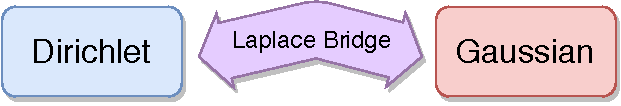
\includegraphics[width=0.7\textwidth]{../figures/Laplace_Bridge_sketch.pdf}
	\end{figure}
	\begin{itemize}
		\item The Dirichlet in the inverse softmax basis approximates a Gaussian
		\item Via the Laplace approximation in the transformed basis we can create a closed-form transformation $\alpha \rightarrow (\mu, \Sigma)$.
		\item We can also construct an inverse of this transformation $(\mu, \Sigma) \rightarrow \alpha$
		\item In total, we have a \textbf{fast} way to transform between the parameters of a Dirichlet and a Gaussian
	\end{itemize}
\end{frame}

%%%%%%%%%%%%%%%%%%%%%%%%%

\begin{frame}\frametitle{The Laplace Bridge}
	\framesubtitle{Application to Neural Networks}
	\begin{figure}
		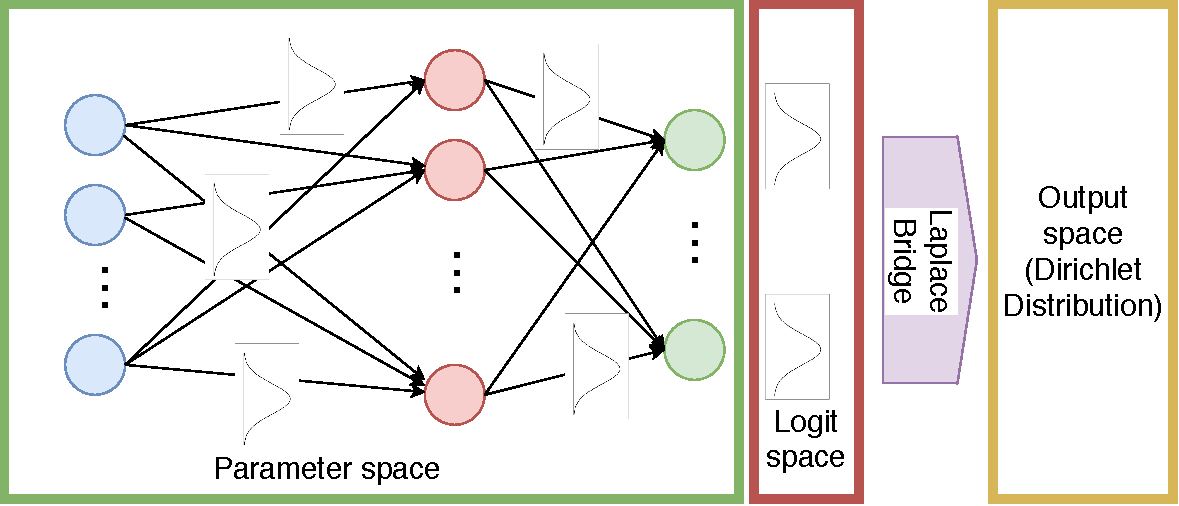
\includegraphics[width=\textwidth]{../figures/GaussNN_LaplaceBridge.pdf}
	\end{figure}
\end{frame}

%%%%%%%%%%%%%%%%%%%%%%%%%
%     Experiments
%%%%%%%%%%%%%%%%%%%%%%%%%
\blackslidetext{\center{\large\textbf{Experiments}}}

\begin{frame}\frametitle{A sanity check}
	\framesubtitle{Samples from a 3D Gaussian + Softmax vs. Dirichlet}
	\begin{figure}
		\centering
		\subfloat{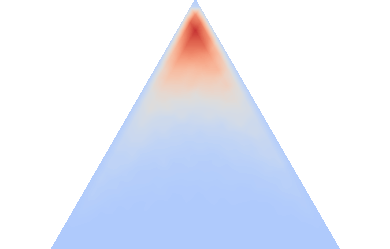
\includegraphics[width=0.18\textwidth]{../figures/sMAP/sMAP_Gaussian_coolwarm_0.png}}
		\subfloat{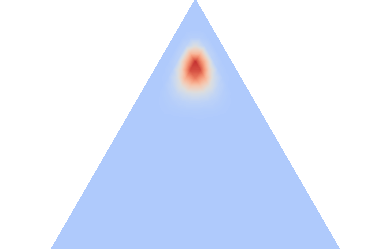
\includegraphics[width=0.18\textwidth]{../figures/sMAP/sMAP_Gaussian_coolwarm_1.png}}
		\subfloat{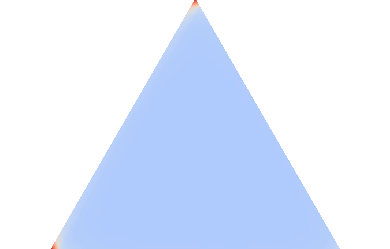
\includegraphics[width=0.18\textwidth]{../figures/Uncertainty/Uncertainty_Gaussian_coolwarm_0.png}}
		\subfloat{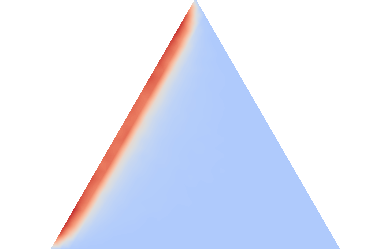
\includegraphics[width=0.18\textwidth]{../figures/Uncertainty/Uncertainty_Gaussian_coolwarm_1.png}}
		\subfloat{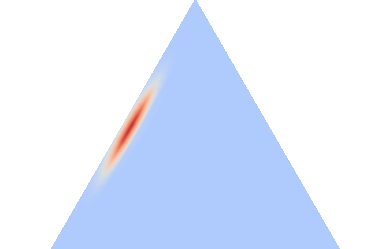
\includegraphics[width=0.18\textwidth]{../figures/Uncertainty/Uncertainty_Gaussian_coolwarm_2.png}}
		
		\vspace{10pt}
		\setcounter{subfigure}{0}
		
		\subfloat{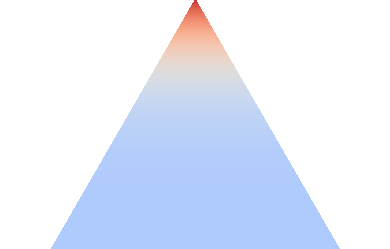
\includegraphics[width=0.18\textwidth]{../figures/sMAP/sMAP_Dirichlet_coolwarm_0.png}}
		\subfloat{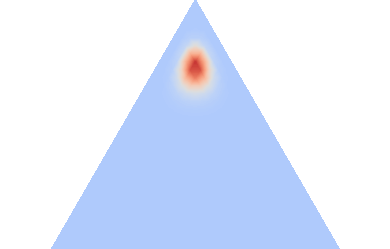
\includegraphics[width=0.18\textwidth]{../figures/sMAP/sMAP_Dirichlet_coolwarm_1.png}}
		\subfloat{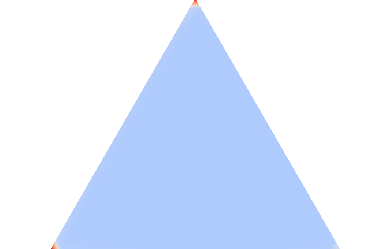
\includegraphics[width=0.18\textwidth]{../figures/Uncertainty/Uncertainty_Dirichlet_coolwarm_0.png}}
		\subfloat{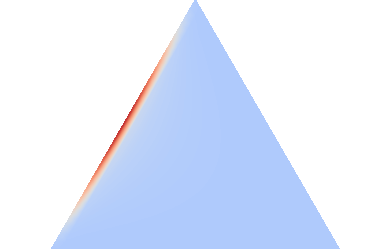
\includegraphics[width=0.18\textwidth]{../figures/Uncertainty/Uncertainty_Dirichlet_coolwarm_1.png}}
		\subfloat{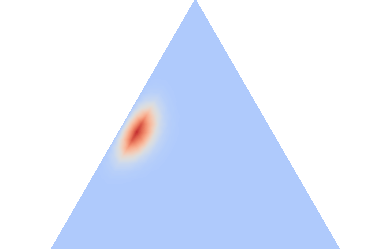
\includegraphics[width=0.18\textwidth]{../figures/Uncertainty/Uncertainty_Dirichlet_coolwarm_2.png}}
	\end{figure}
\end{frame}

%%%%%%%%%%%%%%%%%%%%%%%%%

\setlength{\figwidth}{0.9\textwidth}
\setlength{\figheight}{0.7\textheight}

\begin{frame}\frametitle{MNIST}
	\framesubtitle{Train on 0,1,2; test on 0-9}
	\begin{figure}
		%\includegraphics[width=0.9\textwidth]{imagefile}
		% This file was created by tikzplotlib v0.8.2.
\begin{tikzpicture}

\begin{axis}[
height=\figheight,
legend cell align={left},
legend pos=north west,
legend style={draw=white!80.0!black},
tick align=outside,
tick pos=both,
width=\figwidth,
x grid style={white!69.01960784313725!black},
xlabel={MNIST Class},
xmin=-0.45, xmax=9.45,
xtick align=outside,
xtick pos=left,
xtick style={color=black},
y grid style={white!69.01960784313725!black},
ylabel={Mean Variance},
ymin=-0.0054625256190775, ymax=0.120914868576801,
ytick align=outside,
ytick pos=left,
ytick style={color=black},
ytick={-0.02,0,0.02,0.04,0.06,0.08,0.1,0.12,0.14},
yticklabels={−0.02,0.00,0.02,0.04,0.06,0.08,0.10,0.12,0.14}
]
\addplot [semithick, red, mark=*, mark size=3, mark options={solid}, only marks]
table {%
0 0.000485580181702971
1 0.00123255501966923
2 0.000281901389826089
};
\addlegendentry{In Dist}
\addplot [semithick, blue, mark=*, mark size=3, mark options={solid}, only marks]
table {%
3 0.0408964194357395
4 0.115170441567898
5 0.0661771073937416
6 0.039771307259798
7 0.0582874082028866
8 0.039117556065321
9 0.0806255489587784
};
\addlegendentry{Out Dist}
\end{axis}

\end{tikzpicture}
	\end{figure}
\end{frame}

%%%%%%%%%%%%%%%%%%%%%%%%%

\begin{frame}\frametitle{Speedtest - I}
	\framesubtitle{KL divergence vs. number of samples}
	\begin{figure}
		%\includegraphics[width=0.9\textwidth]{imagefile}
		% This file was created by tikzplotlib v0.8.2.
\begin{tikzpicture}

\definecolor{color0}{rgb}{1,0.647058823529412,0}
\definecolor{color1}{rgb}{0.501960784313725,0,0.501960784313725}
\definecolor{color2}{rgb}{0.647058823529412,0.164705882352941,0.164705882352941}

\begin{axis}[
height=\figheight,
legend cell align={left},
legend pos=north east,
legend style={draw=white!80.0!black},
log basis x={10},
tick pos=both,
width=\figwidth,
x grid style={white!69.01960784313725!black},
xlabel={Number of Samples},
xmin=0.562341325190349, xmax=177827.941003892,
xmode=log,
xtick align=inside,
xtick pos=left,
xtick style={color=black},
xtick={0.01,0.1,1,10,100,1000,10000,100000,1000000,10000000},
xticklabels={\(\displaystyle {10^{-2}}\),\(\displaystyle {10^{-1}}\),\(\displaystyle {10^{0}}\),\(\displaystyle {10^{1}}\),\(\displaystyle {10^{2}}\),\(\displaystyle {10^{3}}\),\(\displaystyle {10^{4}}\),\(\displaystyle {10^{5}}\),\(\displaystyle {10^{6}}\),\(\displaystyle {10^{7}}\)},
y grid style={white!69.01960784313725!black},
ylabel={KL Divergence},
ymin=-2.15254313802994, ymax=45.2034058986287,
ytick align=inside,
ytick pos=left,
ytick style={color=black}
]
\path [draw=blue, very thick]
(axis cs:1,41.3722702823216)
--(axis cs:1,41.3722702823216);

\path [draw=blue, very thick]
(axis cs:5,38.8233030125781)
--(axis cs:5,39.0591480735509);

\path [draw=blue, very thick]
(axis cs:10,35.267481412799)
--(axis cs:10,36.9329452871732);

\path [draw=blue, very thick]
(axis cs:25,29.1319009116699)
--(axis cs:25,31.6236385020272);

\path [draw=blue, very thick]
(axis cs:50,21.304965177582)
--(axis cs:50,24.1591645143799);

\path [draw=blue, very thick]
(axis cs:75,16.6383771143455)
--(axis cs:75,17.6845412745849);

\path [draw=blue, very thick]
(axis cs:100,12.4928905678809)
--(axis cs:100,15.2919407971065);

\path [draw=blue, very thick]
(axis cs:250,5.67699779647913)
--(axis cs:250,6.30875076113871);

\path [draw=blue, very thick]
(axis cs:500,2.26833776833095)
--(axis cs:500,3.34790920534813);

\path [draw=blue, very thick]
(axis cs:750,1.58530484653685)
--(axis cs:750,2.09189915175033);

\path [draw=blue, very thick]
(axis cs:1000,1.09512113945861)
--(axis cs:1000,1.25898831175564);

\path [draw=blue, very thick]
(axis cs:2500,0.370662637687383)
--(axis cs:2500,0.499793601288633);

\path [draw=blue, very thick]
(axis cs:5000,0.231181061336582)
--(axis cs:5000,0.279238460248237);

\path [draw=blue, very thick]
(axis cs:7500,0.139836470091655)
--(axis cs:7500,0.164872822137191);

\path [draw=blue, very thick]
(axis cs:10000,0.084337512184737)
--(axis cs:10000,0.106616449204758);

\path [draw=blue, very thick]
(axis cs:25000,0.0358771476288979)
--(axis cs:25000,0.0424959131298682);

\path [draw=blue, very thick]
(axis cs:50000,0.0178279890062826)
--(axis cs:50000,0.0233430690525671);

\path [draw=blue, very thick]
(axis cs:75000,0.0120503163100018)
--(axis cs:75000,0.0172004825023739);

\path [draw=blue, very thick]
(axis cs:100000,0.0100070768674574)
--(axis cs:100000,0.0125073077088456);

\path [draw=color0, very thick]
(axis cs:1,43.0508627605988)
--(axis cs:1,43.0508627605988);

\path [draw=color0, very thick]
(axis cs:5,32.9164696418971)
--(axis cs:5,38.558368232746);

\path [draw=color0, very thick]
(axis cs:10,29.3357170610752)
--(axis cs:10,34.3925399576855);

\path [draw=color0, very thick]
(axis cs:25,18.1543726761943)
--(axis cs:25,23.7064784539694);

\path [draw=color0, very thick]
(axis cs:50,14.1139008509748)
--(axis cs:50,16.7560266158067);

\path [draw=color0, very thick]
(axis cs:75,10.7357449683897)
--(axis cs:75,12.5322548346119);

\path [draw=color0, very thick]
(axis cs:100,9.58497879599963)
--(axis cs:100,10.3003525490437);

\path [draw=color0, very thick]
(axis cs:250,5.67213818176429)
--(axis cs:250,6.88573036979303);

\path [draw=color0, very thick]
(axis cs:500,3.8340459965373)
--(axis cs:500,4.32652116301364);

\path [draw=color0, very thick]
(axis cs:750,2.54909605301928)
--(axis cs:750,3.3883456915885);

\path [draw=color0, very thick]
(axis cs:1000,2.22816978651728)
--(axis cs:1000,2.47026168174398);

\path [draw=color0, very thick]
(axis cs:2500,1.07000462007234)
--(axis cs:2500,1.28476288361077);

\path [draw=color0, very thick]
(axis cs:5000,0.495096355743176)
--(axis cs:5000,0.554422544733448);

\path [draw=color0, very thick]
(axis cs:7500,0.328971266525497)
--(axis cs:7500,0.395221842442994);

\path [draw=color0, very thick]
(axis cs:10000,0.2305577201191)
--(axis cs:10000,0.294069003433279);

\path [draw=color0, very thick]
(axis cs:25000,0.0937054047200392)
--(axis cs:25000,0.100406236295138);

\path [draw=color0, very thick]
(axis cs:50000,0.0370128142188019)
--(axis cs:50000,0.0451002552278923);

\path [draw=color0, very thick]
(axis cs:75000,0.0228132706100869)
--(axis cs:75000,0.024795862739992);

\path [draw=color0, very thick]
(axis cs:100000,0.0153163404700447)
--(axis cs:100000,0.0202666204467783);

\path [draw=green!50.19607843137255!black, very thick]
(axis cs:1,42.93349488395)
--(axis cs:1,42.93349488395);

\path [draw=green!50.19607843137255!black, very thick]
(axis cs:5,37.0750021059541)
--(axis cs:5,38.4748201996713);

\path [draw=green!50.19607843137255!black, very thick]
(axis cs:10,34.2358799246236)
--(axis cs:10,36.0148853930903);

\path [draw=green!50.19607843137255!black, very thick]
(axis cs:25,24.3716676967715)
--(axis cs:25,26.5337565446618);

\path [draw=green!50.19607843137255!black, very thick]
(axis cs:50,18.6676069935368)
--(axis cs:50,19.6412544376819);

\path [draw=green!50.19607843137255!black, very thick]
(axis cs:75,10.6572615218368)
--(axis cs:75,14.6737306768942);

\path [draw=green!50.19607843137255!black, very thick]
(axis cs:100,7.66062640020415)
--(axis cs:100,9.54815976735437);

\path [draw=green!50.19607843137255!black, very thick]
(axis cs:250,2.98932209269546)
--(axis cs:250,4.25632264994355);

\path [draw=green!50.19607843137255!black, very thick]
(axis cs:500,0.843772314988995)
--(axis cs:500,1.2663946119617);

\path [draw=green!50.19607843137255!black, very thick]
(axis cs:750,0.577993218332512)
--(axis cs:750,0.875373247983097);

\path [draw=green!50.19607843137255!black, very thick]
(axis cs:1000,0.301307271541921)
--(axis cs:1000,0.57281390854175);

\path [draw=green!50.19607843137255!black, very thick]
(axis cs:2500,0.175692102095908)
--(axis cs:2500,0.245401076384385);

\path [draw=green!50.19607843137255!black, very thick]
(axis cs:5000,0.0814301408001577)
--(axis cs:5000,0.140221637810137);

\path [draw=green!50.19607843137255!black, very thick]
(axis cs:7500,0.0512626639403834)
--(axis cs:7500,0.065374162994615);

\path [draw=green!50.19607843137255!black, very thick]
(axis cs:10000,0.0406086501456689)
--(axis cs:10000,0.062530297040719);

\path [draw=green!50.19607843137255!black, very thick]
(axis cs:25000,0.0185861002926118)
--(axis cs:25000,0.0263330151450657);

\path [draw=green!50.19607843137255!black, very thick]
(axis cs:50000,0.00797514769943751)
--(axis cs:50000,0.0100283052176679);

\path [draw=green!50.19607843137255!black, very thick]
(axis cs:75000,0.0069841735211465)
--(axis cs:75000,0.00894536725832454);

\path [draw=green!50.19607843137255!black, very thick]
(axis cs:100000,0.00470287418533706)
--(axis cs:100000,0.00678371869152951);

\path [draw=blue, draw opacity=0.7, semithick]
(axis cs:25000,0)
--(axis cs:25000,7);

\path [draw=color0, draw opacity=0.7, semithick]
(axis cs:5000,0)
--(axis cs:5000,7);

\path [draw=green!50.19607843137255!black, draw opacity=0.7, semithick]
(axis cs:500,0)
--(axis cs:500,7);

\addplot [semithick, red, mark=*, mark size=3, mark options={solid}, only marks]
table {%
1 0.0881709970024221
};
\addlegendentry{Laplace Bridge}
\addplot [semithick, color1, mark=*, mark size=3, mark options={solid}, only marks, forget plot]
table {%
1 0.707545925704699
};
\addplot [semithick, color2, mark=*, mark size=3, mark options={solid}, only marks, forget plot]
table {%
1 1.7655057604949
};
\addplot [very thick, red, opacity=0.5, dash pattern=on 1pt off 3pt on 3pt off 3pt, forget plot]
table {%
1 0.0881709970024221
25000 0.0881709970024221
};
\addplot [very thick, color1, opacity=0.5, dash pattern=on 1pt off 3pt on 3pt off 3pt, forget plot]
table {%
1 0.707545925704699
5000 0.707545925704699
};
\addplot [very thick, color2, opacity=0.5, dash pattern=on 1pt off 3pt on 3pt off 3pt, forget plot]
table {%
1 1.7655057604949
500 1.7655057604949
};
\addplot [very thick, blue]
table {%
1 41.3722702823216
5 38.9412255430645
10 36.1002133499861
25 30.3777697068485
50 22.7320648459809
75 17.1614591944652
100 13.8924156824937
250 5.99287427880892
500 2.80812348683954
750 1.83860199914359
1000 1.17705472560713
2500 0.435228119488008
5000 0.255209760792409
7500 0.152354646114423
10000 0.0954769806947477
25000 0.039186530379383
50000 0.0205855290294249
75000 0.0146253994061879
100000 0.0112571922881515
};
\addlegendentry{Monte Carlo}
\addplot [very thick, color0]
table {%
1 43.0508627605988
5 35.7374189373216
10 31.8641285093803
25 20.9304255650818
50 15.4349637333907
75 11.6339999015008
100 9.94266567252169
250 6.27893427577866
500 4.08028357977547
750 2.96872087230389
1000 2.34921573413063
2500 1.17738375184156
5000 0.524759450238312
7500 0.362096554484246
10000 0.262313361776189
25000 0.0970558205075884
50000 0.0410565347233471
75000 0.0238045666750394
100000 0.0177914804584115
};
\addlegendentry{Monte Carlo}
\addplot [very thick, green!50.19607843137255!black]
table {%
1 42.93349488395
5 37.7749111528127
10 35.1253826588569
25 25.4527121207166
50 19.1544307156093
75 12.6654960993655
100 8.60439308377926
250 3.6228223713195
500 1.05508346347535
750 0.726683233157805
1000 0.437060590041835
2500 0.210546589240146
5000 0.110825889305147
7500 0.0583184134674992
10000 0.0515694735931939
25000 0.0224595577188388
50000 0.00900172645855269
75000 0.00796477038973552
100000 0.00574329643843329
};
\addlegendentry{Monte Carlo}
\end{axis}

\end{tikzpicture}
	\end{figure}
\end{frame}

%%%%%%%%%%%%%%%%%%%%%%%%%

\begin{frame}\frametitle{Speedtest - II}
	\framesubtitle{KL divergence vs. wall-clock time}
	\begin{figure}
		%\includegraphics[width=0.9\textwidth]{imagefile}
		% This file was created by tikzplotlib v0.8.2.
\begin{tikzpicture}

\definecolor{color0}{rgb}{1,0.647058823529412,0}
\definecolor{color1}{rgb}{0.501960784313725,0,0.501960784313725}
\definecolor{color2}{rgb}{0.647058823529412,0.164705882352941,0.164705882352941}

\begin{axis}[
height=\figheight,
legend cell align={left},
legend pos=north east,
legend style={draw=white!80.0!black},
log basis x={10},
tick pos=both,
width=\figwidth,
x grid style={white!69.01960784313725!black},
xlabel={Time in s},
xmin=0.000219164109011124, xmax=1.57720836573318,
xmode=log,
xtick align=inside,
xtick pos=left,
xtick style={color=black},
xtick={1e-05,0.0001,0.001,0.01,0.1,1,10,100},
xticklabels={\(\displaystyle {10^{-5}}\),\(\displaystyle {10^{-4}}\),\(\displaystyle {10^{-3}}\),\(\displaystyle {10^{-2}}\),\(\displaystyle {10^{-1}}\),\(\displaystyle {10^{0}}\),\(\displaystyle {10^{1}}\),\(\displaystyle {10^{2}}\)},
y grid style={white!69.01960784313725!black},
ylabel={KL Divergence},
ymin=-2.15254313802994, ymax=45.2034058986287,
ytick align=inside,
ytick pos=left,
ytick style={color=black}
]
\path [draw=blue, very thick]
(axis cs:0.000347699400003876,41.3722702823216)
--(axis cs:0.000347699400003876,41.3722702823216);

\path [draw=blue, very thick]
(axis cs:0.00034134719999912,38.8233030125781)
--(axis cs:0.00034134719999912,39.0591480735509);

\path [draw=blue, very thick]
(axis cs:0.000392544400003203,35.267481412799)
--(axis cs:0.000392544400003203,36.9329452871732);

\path [draw=blue, very thick]
(axis cs:0.000552010000004088,29.1319009116699)
--(axis cs:0.000552010000004088,31.6236385020272);

\path [draw=blue, very thick]
(axis cs:0.000753213599996627,21.304965177582)
--(axis cs:0.000753213599996627,24.1591645143799);

\path [draw=blue, very thick]
(axis cs:0.000953311199998552,16.6383771143455)
--(axis cs:0.000953311199998552,17.6845412745849);

\path [draw=blue, very thick]
(axis cs:0.00117008360000312,12.4928905678809)
--(axis cs:0.00117008360000312,15.2919407971065);

\path [draw=blue, very thick]
(axis cs:0.002496716200001,5.67699779647913)
--(axis cs:0.002496716200001,6.30875076113871);

\path [draw=blue, very thick]
(axis cs:0.00535201260000235,2.26833776833095)
--(axis cs:0.00535201260000235,3.34790920534813);

\path [draw=blue, very thick]
(axis cs:0.00664694479999781,1.58530484653685)
--(axis cs:0.00664694479999781,2.09189915175033);

\path [draw=blue, very thick]
(axis cs:0.00847694239999726,1.09512113945861)
--(axis cs:0.00847694239999726,1.25898831175564);

\path [draw=blue, very thick]
(axis cs:0.0210023156000034,0.370662637687383)
--(axis cs:0.0210023156000034,0.499793601288633);

\path [draw=blue, very thick]
(axis cs:0.0419743216000043,0.231181061336582)
--(axis cs:0.0419743216000043,0.279238460248237);

\path [draw=blue, very thick]
(axis cs:0.124657420200003,0.139836470091655)
--(axis cs:0.124657420200003,0.164872822137191);

\path [draw=blue, very thick]
(axis cs:0.171043202599995,0.084337512184737)
--(axis cs:0.171043202599995,0.106616449204758);

\path [draw=blue, very thick]
(axis cs:0.414873980599999,0.0358771476288979)
--(axis cs:0.414873980599999,0.0424959131298682);

\path [draw=blue, very thick]
(axis cs:0.622958016799997,0.0178279890062826)
--(axis cs:0.622958016799997,0.0233430690525671);

\path [draw=blue, very thick]
(axis cs:0.843133083400001,0.0120503163100018)
--(axis cs:0.843133083400001,0.0172004825023739);

\path [draw=blue, very thick]
(axis cs:1.0460591128,0.0100070768674574)
--(axis cs:1.0460591128,0.0125073077088456);

\path [draw=color0, very thick]
(axis cs:0.000328165600001284,43.0508627605988)
--(axis cs:0.000328165600001284,43.0508627605988);

\path [draw=color0, very thick]
(axis cs:0.000356451800006141,32.9164696418971)
--(axis cs:0.000356451800006141,38.558368232746);

\path [draw=color0, very thick]
(axis cs:0.000429854600000112,29.3357170610752)
--(axis cs:0.000429854600000112,34.3925399576855);

\path [draw=color0, very thick]
(axis cs:0.000522573999997178,18.1543726761943)
--(axis cs:0.000522573999997178,23.7064784539694);

\path [draw=color0, very thick]
(axis cs:0.000754682999999545,14.1139008509748)
--(axis cs:0.000754682999999545,16.7560266158067);

\path [draw=color0, very thick]
(axis cs:0.000940918799997803,10.7357449683897)
--(axis cs:0.000940918799997803,12.5322548346119);

\path [draw=color0, very thick]
(axis cs:0.00114930980000025,9.58497879599963)
--(axis cs:0.00114930980000025,10.3003525490437);

\path [draw=color0, very thick]
(axis cs:0.00242379079999608,5.67213818176429)
--(axis cs:0.00242379079999608,6.88573036979303);

\path [draw=color0, very thick]
(axis cs:0.00461063900000624,3.8340459965373)
--(axis cs:0.00461063900000624,4.32652116301364);

\path [draw=color0, very thick]
(axis cs:0.00645582219999738,2.54909605301928)
--(axis cs:0.00645582219999738,3.3883456915885);

\path [draw=color0, very thick]
(axis cs:0.008581556799993,2.22816978651728)
--(axis cs:0.008581556799993,2.47026168174398);

\path [draw=color0, very thick]
(axis cs:0.0208941222000035,1.07000462007234)
--(axis cs:0.0208941222000035,1.28476288361077);

\path [draw=color0, very thick]
(axis cs:0.041313977599998,0.495096355743176)
--(axis cs:0.041313977599998,0.554422544733448);

\path [draw=color0, very thick]
(axis cs:0.135163926200001,0.328971266525497)
--(axis cs:0.135163926200001,0.395221842442994);

\path [draw=color0, very thick]
(axis cs:0.170700134799996,0.2305577201191)
--(axis cs:0.170700134799996,0.294069003433279);

\path [draw=color0, very thick]
(axis cs:0.410511967799992,0.0937054047200392)
--(axis cs:0.410511967799992,0.100406236295138);

\path [draw=color0, very thick]
(axis cs:0.616218821999996,0.0370128142188019)
--(axis cs:0.616218821999996,0.0451002552278923);

\path [draw=color0, very thick]
(axis cs:0.827729683600002,0.0228132706100869)
--(axis cs:0.827729683600002,0.024795862739992);

\path [draw=color0, very thick]
(axis cs:1.0407518114,0.0153163404700447)
--(axis cs:1.0407518114,0.0202666204467783);

\path [draw=green!50.19607843137255!black, very thick]
(axis cs:0.000351066999994032,42.93349488395)
--(axis cs:0.000351066999994032,42.93349488395);

\path [draw=green!50.19607843137255!black, very thick]
(axis cs:0.000371052200007682,37.0750021059541)
--(axis cs:0.000371052200007682,38.4748201996713);

\path [draw=green!50.19607843137255!black, very thick]
(axis cs:0.000424890399990829,34.2358799246236)
--(axis cs:0.000424890399990829,36.0148853930903);

\path [draw=green!50.19607843137255!black, very thick]
(axis cs:0.000527281800000878,24.3716676967715)
--(axis cs:0.000527281800000878,26.5337565446618);

\path [draw=green!50.19607843137255!black, very thick]
(axis cs:0.000747899799998208,18.6676069935368)
--(axis cs:0.000747899799998208,19.6412544376819);

\path [draw=green!50.19607843137255!black, very thick]
(axis cs:0.00145907819999707,10.6572615218368)
--(axis cs:0.00145907819999707,14.6737306768942);

\path [draw=green!50.19607843137255!black, very thick]
(axis cs:0.00118932279999768,7.66062640020415)
--(axis cs:0.00118932279999768,9.54815976735437);

\path [draw=green!50.19607843137255!black, very thick]
(axis cs:0.00242782120000271,2.98932209269546)
--(axis cs:0.00242782120000271,4.25632264994355);

\path [draw=green!50.19607843137255!black, very thick]
(axis cs:0.00457135460000728,0.843772314988995)
--(axis cs:0.00457135460000728,1.2663946119617);

\path [draw=green!50.19607843137255!black, very thick]
(axis cs:0.00679406500000397,0.577993218332512)
--(axis cs:0.00679406500000397,0.875373247983097);

\path [draw=green!50.19607843137255!black, very thick]
(axis cs:0.00846984139999591,0.301307271541921)
--(axis cs:0.00846984139999591,0.57281390854175);

\path [draw=green!50.19607843137255!black, very thick]
(axis cs:0.020912775400005,0.175692102095908)
--(axis cs:0.020912775400005,0.245401076384385);

\path [draw=green!50.19607843137255!black, very thick]
(axis cs:0.042248899600007,0.0814301408001577)
--(axis cs:0.042248899600007,0.140221637810137);

\path [draw=green!50.19607843137255!black, very thick]
(axis cs:0.127125916000007,0.0512626639403834)
--(axis cs:0.127125916000007,0.065374162994615);

\path [draw=green!50.19607843137255!black, very thick]
(axis cs:0.167992996799998,0.0406086501456689)
--(axis cs:0.167992996799998,0.062530297040719);

\path [draw=green!50.19607843137255!black, very thick]
(axis cs:0.407860939999999,0.0185861002926118)
--(axis cs:0.407860939999999,0.0263330151450657);

\path [draw=green!50.19607843137255!black, very thick]
(axis cs:0.617105053200001,0.00797514769943751)
--(axis cs:0.617105053200001,0.0100283052176679);

\path [draw=green!50.19607843137255!black, very thick]
(axis cs:0.830234605999996,0.0069841735211465)
--(axis cs:0.830234605999996,0.00894536725832454);

\path [draw=green!50.19607843137255!black, very thick]
(axis cs:1.0533324218,0.00470287418533706)
--(axis cs:1.0533324218,0.00678371869152951);

\path [draw=blue, draw opacity=0.7, semithick]
(axis cs:0.414873980599999,0)
--(axis cs:0.414873980599999,7);

\path [draw=color0, draw opacity=0.7, semithick]
(axis cs:0.041313977599998,0)
--(axis cs:0.041313977599998,7);

\path [draw=green!50.19607843137255!black, draw opacity=0.7, semithick]
(axis cs:0.00457135460000728,0)
--(axis cs:0.00457135460000728,7);

\addplot [semithick, red, mark=*, mark size=3, mark options={solid}, only marks]
table {%
0.000628673999999663 0.0881709970024221
};
\addlegendentry{Laplace Bridge}
\addplot [semithick, color1, mark=*, mark size=3, mark options={solid}, only marks, forget plot]
table {%
0.000856472999999802 0.707545925704699
};
\addplot [semithick, color2, mark=*, mark size=3, mark options={solid}, only marks, forget plot]
table {%
0.000598666999999331 1.7655057604949
};
\addplot [very thick, red, opacity=0.5, dash pattern=on 1pt off 3pt on 3pt off 3pt, forget plot]
table {%
0.000628673999999663 0.0881709970024221
0.414873980599999 0.0881709970024221
};
\addplot [very thick, color1, opacity=0.5, dash pattern=on 1pt off 3pt on 3pt off 3pt, forget plot]
table {%
0.000856472999999802 0.707545925704699
0.041313977599998 0.707545925704699
};
\addplot [very thick, color2, opacity=0.5, dash pattern=on 1pt off 3pt on 3pt off 3pt, forget plot]
table {%
0.000598666999999331 1.7655057604949
0.00457135460000728 1.7655057604949
};
\addplot [very thick, blue]
table {%
0.000347699400003876 41.3722702823216
0.00034134719999912 38.9412255430645
0.000392544400003203 36.1002133499861
0.000552010000004088 30.3777697068485
0.000753213599996627 22.7320648459809
0.000953311199998552 17.1614591944652
0.00117008360000312 13.8924156824937
0.002496716200001 5.99287427880892
0.00535201260000235 2.80812348683954
0.00664694479999781 1.83860199914359
0.00847694239999726 1.17705472560713
0.0210023156000034 0.435228119488008
0.0419743216000043 0.255209760792409
0.124657420200003 0.152354646114423
0.171043202599995 0.0954769806947477
0.414873980599999 0.039186530379383
0.622958016799997 0.0205855290294249
0.843133083400001 0.0146253994061879
1.0460591128 0.0112571922881515
};
\addlegendentry{Monte Carlo}
\addplot [very thick, color0]
table {%
0.000328165600001284 43.0508627605988
0.000356451800006141 35.7374189373216
0.000429854600000112 31.8641285093803
0.000522573999997178 20.9304255650818
0.000754682999999545 15.4349637333907
0.000940918799997803 11.6339999015008
0.00114930980000025 9.94266567252169
0.00242379079999608 6.27893427577866
0.00461063900000624 4.08028357977547
0.00645582219999738 2.96872087230389
0.008581556799993 2.34921573413063
0.0208941222000035 1.17738375184156
0.041313977599998 0.524759450238312
0.135163926200001 0.362096554484246
0.170700134799996 0.262313361776189
0.410511967799992 0.0970558205075884
0.616218821999996 0.0410565347233471
0.827729683600002 0.0238045666750394
1.0407518114 0.0177914804584115
};
\addlegendentry{Monte Carlo}
\addplot [very thick, green!50.19607843137255!black]
table {%
0.000351066999994032 42.93349488395
0.000371052200007682 37.7749111528127
0.000424890399990829 35.1253826588569
0.000527281800000878 25.4527121207166
0.000747899799998208 19.1544307156093
0.00145907819999707 12.6654960993655
0.00118932279999768 8.60439308377926
0.00242782120000271 3.6228223713195
0.00457135460000728 1.05508346347535
0.00679406500000397 0.726683233157805
0.00846984139999591 0.437060590041835
0.020912775400005 0.210546589240146
0.042248899600007 0.110825889305147
0.127125916000007 0.0583184134674992
0.167992996799998 0.0515694735931939
0.407860939999999 0.0224595577188388
0.617105053200001 0.00900172645855269
0.830234605999996 0.00796477038973552
1.0533324218 0.00574329643843329
};
\addlegendentry{Monte Carlo}
\end{axis}

\end{tikzpicture}
	\end{figure}
\end{frame}

%%%%%%%%%%%%%%%%%%%%%%%%%

\setlength{\figwidth}{0.95\textwidth}
\setlength{\figheight}{0.34\textheight}

\begin{frame}\frametitle{Imagenet}
	\framesubtitle{Using the properties of the Dirichlet - The marginal of a Dirichlet is a Dirichlet}
	\begin{figure}
		\centering
		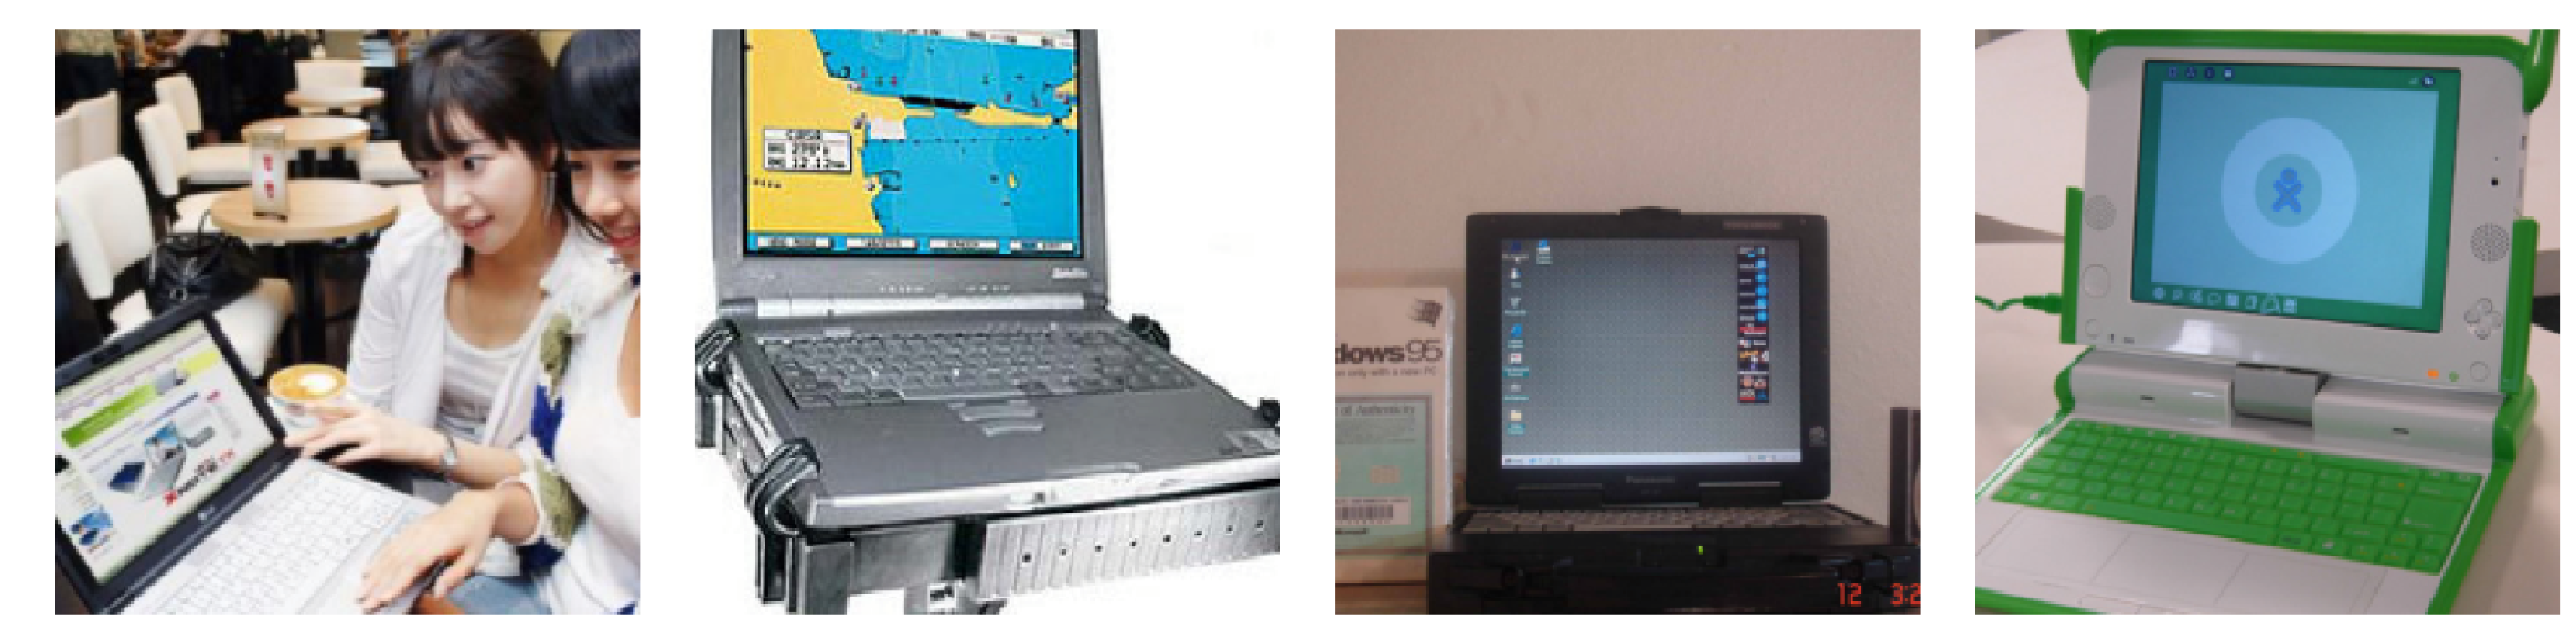
\includegraphics[width=\figwidth,height=\figheight]{../figures/imagenet_images.pdf} \\
		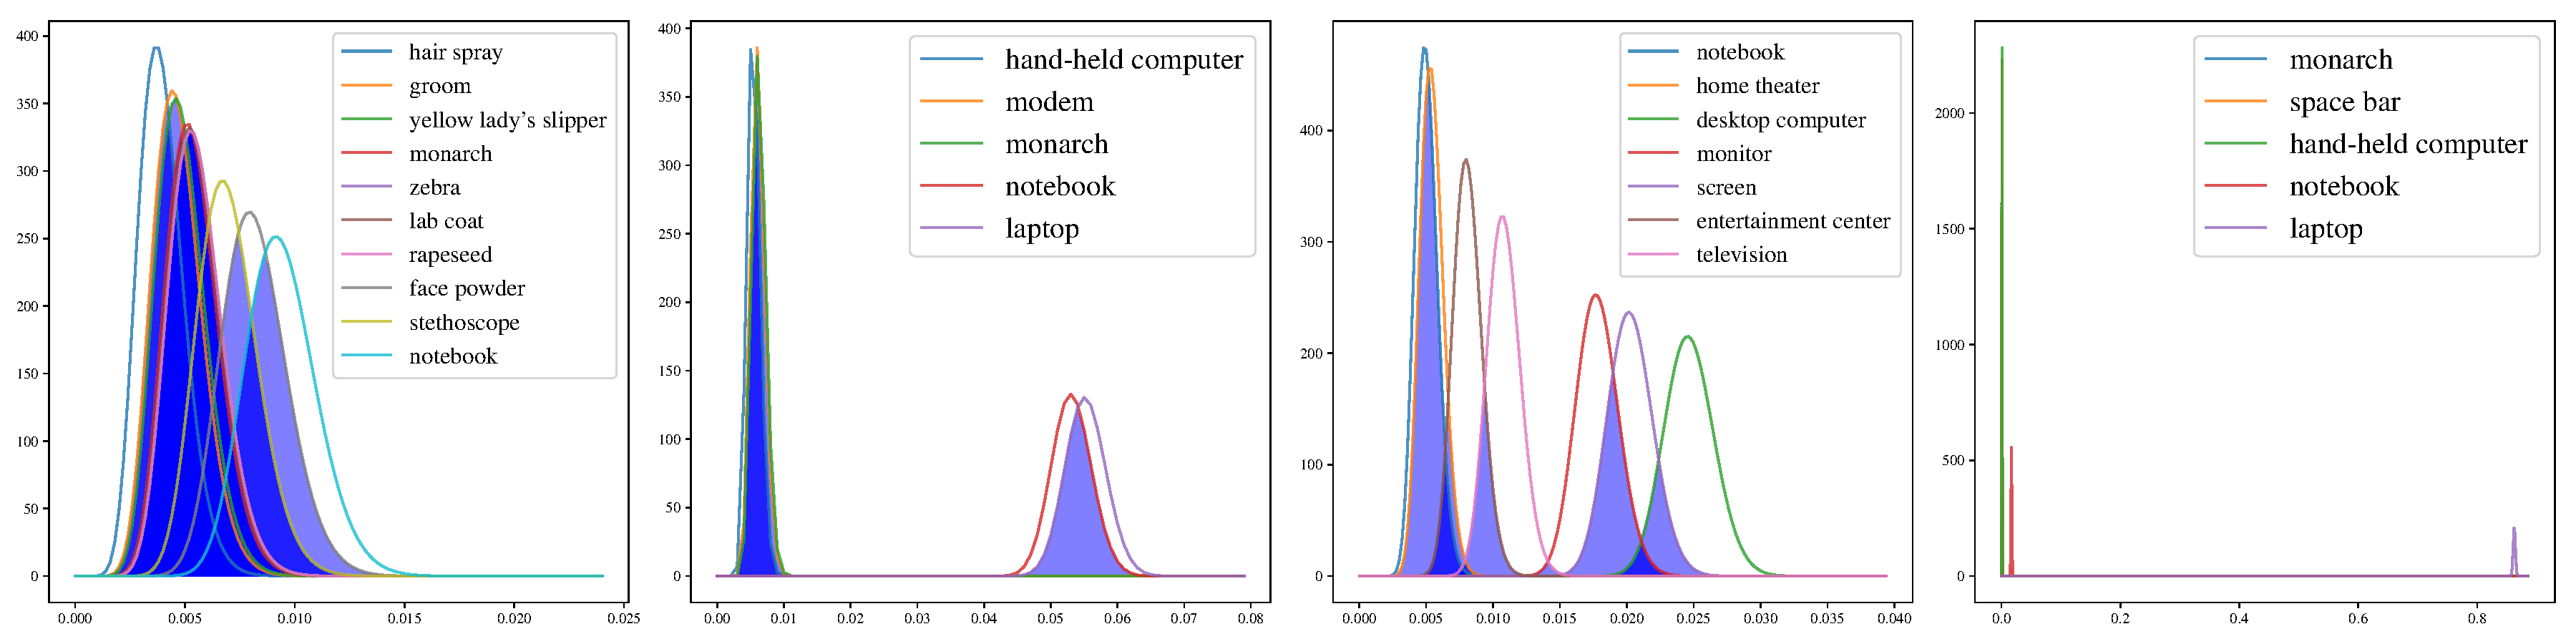
\includegraphics[width=\figwidth,height=\figheight]{../figures/imagenet_marginal_betas.pdf}
	\end{figure}
	We can use the overlap of the distributions to create an uncertainty-aware top-k ranking.
\end{frame}

%%%%%%%%%%%%%%%%%%%%%%%%%

\setlength{\figwidth}{0.95\textwidth}
\setlength{\figheight}{0.6\textheight}

\begin{frame}\frametitle{Imagenet - II}
	\framesubtitle{How good is the flexible top-k ranking?}
	\begin{figure}
		\centering
		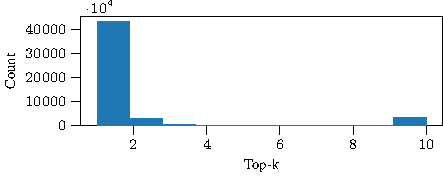
\includegraphics[width=\figwidth,height=\figheight]{../figures/output-figure4.pdf} 
	\end{figure}
	\begin{itemize}
		\item The original top-$1$ accuracy of DenseNet on ImageNet is $0.744$ and top-$5$ accuracy is $0.919$
		\item The uncertainty-aware top-$k$ accuracy is $0.797$, where $k$ is on average $1.688$
	\end{itemize}
\end{frame}

%%%%%%%%%%%%%%%%%%%%%%%%%

\begin{frame}\frametitle{Out-of-distribution Detection}
	\framesubtitle{Looking at the numbers}
	\resizebox{\textwidth}{!}{% use resizebox with textwidth
		\begin{tabular}{l  l || c c c c | c  c  c  c | c c}
			\toprule
			& & \multicolumn{2}{c}{\textbf{Diag Sampling}} & \multicolumn{2}{c}{\textbf{Diag LB}} &\multicolumn{2}{c}{\textbf{KFAC Sampling}} &  \multicolumn{2}{c}{\textbf{KFAC LB}} & \multicolumn{2}{c}{\textbf{Time in s} $\downarrow$} \\
			\textbf{Train} & \textbf{Test} & \textbf{MMC} $\downarrow$ & \textbf{AUROC} $\uparrow$& \textbf{MMC} $\downarrow$ & \textbf{AUROC} $\uparrow$& \textbf{MMC} $\downarrow$& \textbf{AUROC} $\uparrow$& \textbf{MMC}$\downarrow$ & \textbf{AUROC} $\uparrow$& \textbf{Sampling} & \textbf{LB} \\
			\midrule
			MNIST & MNIST & 0.942 $\pm$ 0.007 & - &  \textbf{0.987} $\pm$ 0.000 & -  & - & - & - & - & 26.8 & \textbf{0.062}\\
			MNIST & FMNIST & 0.397 $\pm$ 0.001 & 0.992 $\pm$ 0.000 & \textbf{0.363} $\pm$ 0.000 & \textbf{0.996} $\pm$ 0.000 & - & - & - & - & 26.8 & \textbf{0.062}\\
			MNIST & notMNIST & \textbf{0.543} $\pm$ 0.000 & 0.960 $\pm$ 0.000 & 0.649 $\pm$ 0.000 & \textbf{0.961} $\pm$ 0.000 & - & - & - & - & 50.3 & \textbf{0.117}\\
			MNIST & KMNIST & \textbf{0.513} $\pm$ 0.001 & \textbf{0.974} $\pm$ 0.000 & 0.637 $\pm$ 0.000 & 0.973 $\pm$ 0.000 & - & - & - & - & 26.9 & \textbf{0.062}\\
			\midrule
			CIFAR-10 & CIFAR-10  & 0.948 $\pm$ 0.000 & -     & \textbf{0.966} $\pm$ 0.000 & -  & 0.857 $\pm$ 0.003 & - & \textbf{0.966} $\pm$ 0.000 & - & 6.58 & \textbf{0.017}\\
			CIFAR-10 & CIFAR-100 & \textbf{0.708} $\pm$ 0.000 & \textbf{0.889} $\pm$ 0.000 & 0.742 $\pm$ 0.000 & 0.866 $\pm$ 0.000 & \textbf{0.562} $\pm$ 0.003 & \textbf{0.880} $\pm$ 0.012 & 0.741 $\pm$ 0.000 & 0.866 $\pm$ 0.000 & 6.59 & \textbf{0.016}\\
			CIFAR-10 & SVHN      & \textbf{0.643}$\pm$ 0.000 & 0.933 $\pm$ 0.000 & 0.647 $\pm$ 0.000 & \textbf{0.934} $\pm$ 0.000& \textbf{0.484} $\pm$ 0.004 & \textbf{0.939} $\pm$ 0.001 & 0.648 $\pm$ 0.003 & 0.934 $\pm$ 0.001 & 17.0 & \textbf{0.040}\\
			\midrule
			SVHN & SVHN       & 0.986 $\pm$ 0.000 &   -   &  \textbf{0.993} $\pm$ 0.000& -     & 0.947 $\pm$ 0.002 & -             & \textbf{0.993}   $\pm$ 0.000          & -     & 17.1 & \textbf{0.042}\\
			SVHN & CIFAR-100  & 0.595 $\pm$ 0.000 & 0.984 $\pm$ 0.000 &  \textbf{0.526} $\pm$ 0.000 & \textbf{0.985} $\pm$ 0.000& \textbf{0.460} $\pm$ 0.004  & \textbf{0.986} $\pm$ 0.001 & 0.527 $\pm$ 0.002 & 0.985 $\pm$ 0.000 & 6.62 & \textbf{0.017}\\
			SVHN & CIFAR-10   & 0.593 $\pm$ 0.000 & 0.984 $\pm$ 0.000&  \textbf{0.520} $\pm$ 0.000 & \textbf{0.987} $\pm$ 0.000 & \textbf{0.458} $\pm$ 0.004  & 0.986 $\pm$ 0.001 & 0.520 $\pm$ 0.002 & \textbf{0.987} $\pm$ 0.000 & 6.62 & \textbf{0.017}\\
			\midrule
			CIFAR-100 & CIFAR-100 & \textbf{0.762} $\pm$ 0.000& - & 0.590 $\pm$ 0.000& - &  0.404 $\pm$ 0.000& - & \textbf{0.593} $\pm$ 0.000& - & 6.76 & \textbf{0.016}\\
			CIFAR-100 & CIFAR-10  & 0.467 $\pm$ 0.000& 0.788 $\pm$ 0.000& \textbf{0.206} $\pm$ 0.000& \textbf{0.791} $\pm$ 0.000& 0.213 $\pm$ 0.000& 0.788 $\pm$ 0.000& \textbf{0.209} $\pm$ 0.000& \textbf{0.791} $\pm$ 0.000 & 6.71 & \textbf{0.017}\\
			CIFAR-100 & SVHN      & 0.461 $\pm$ 0.000& 0.795 $\pm$ 0.000& \textbf{0.170} $\pm$ 0.000& \textbf{0.815} $\pm$ 0.000& 0.180 $\pm$ 0.001 & \textbf{0.838} $\pm$ 0.001 & \textbf{0.173} $\pm$ 0.000 & 0.815 $\pm$ 0.000 & 17.3 & \textbf{0.041}\\
			\bottomrule
		\end{tabular}
	}
	\begin{itemize}
		\item The Laplace Bridge seems to be have better MMC and AUROC compared to sampling from a diagonal Gaussian approximation
		\item The Laplace Bridge is as good as a KFAC approximation
		\item The Laplace Bridge is around 400 times faster on average
	\end{itemize}
\end{frame}

%%%%%%%%%%%%%%%%%%%%%%%%%

\begin{frame}\frametitle{Conclusions}
	\framesubtitle{What can or can't the Laplace Bridge achieve in the context of BNNs?}
	\begin{itemize}
		\item The Laplace Bridge improves an important part of Bayesian Neural Network inference for classification (fast \& non-invasive)
		\item The Dirichlet distribution has some additional interesting use cases (e.g. the top-k ranking)
		\item It will not revolutionize BNNs; it is just one piece in the larger puzzle
	\end{itemize}
\end{frame}

\blackslidetext{\center{\large\textbf{Questions?}}}

%%%%%%%%%%%%%%%%%%%%%%%%%
%     Future 
%%%%%%%%%%%%%%%%%%%%%%%%%

\blackslidetext{\center{\large\textbf{Future}}}

\begin{frame}\frametitle{The generalized Laplace Bridge}
	\framesubtitle{Looking at the larger pattern}
	\begin{itemize}
		\item Similar ``Bridges'' can be found for all exponential families.
		\item Develop a general theoretically grounded framework for the general Laplace Bridge
		\item Compute KL-divergences in the different basis
	\end{itemize}
\end{frame}

%%%%%%%%%%%%%%%%%%%%%%%%%

\begin{frame}\frametitle{The generalized Laplace Bridge}
	\framesubtitle{So what?}
	\textbf{Implications:} (with a small error)
	\begin{itemize}
		\item All exponential families can be transformed to Gaussians
		\item All exponential families can be transformed to each other
		\item All exponential families are conjugate priors for each other
	\end{itemize}
\end{frame}

%%%%%%%%%%%%%%%%%%%%%%%%%
%     Backup
%%%%%%%%%%%%%%%%%%%%%%%%%

\blackslidetext{\center{\textbf{Backup}}}

\begin{frame}\frametitle{Backup}
	\framesubtitle{Laplace approximations of a neural network}
	\begin{equation}
	p(c | x) = \mathcal{N}(x; f(x,w_\text{MAP}), J(x)^T H^{-1} J(x))
	\label{eq:LANN}
	\end{equation}
	\begin{itemize}
		\item $f(x; w_\text{MAP})$ is the network output induced by the MAP estimate $w_\text{MAP}$.
		\item $J(x) = \frac{\partial f(x, w_{\text{MAP}})}{\partial w} \in \mathbb{R}^{K\times P}$ is the Jacobian of the network 
		\item $H_{ij} = \frac{\partial^2 \mathcal{L}(f(x), y)}{\partial w_i \partial w_j} \in \mathbb{R}^{P \times P}$ its Hessian. 
		\item $K, P$ are the number of classes and parameters of the network respectively.
	\end{itemize}
\end{frame}

%%%%%%%%%%%%%%%%%%%%%%%%%

\begin{frame}\frametitle{Backup}
	\framesubtitle{A theoretical bound for the transformation}
	\begin{proposition} \label{prop:dir_var_from_gaussian}
		Let $\mathrm{Dir}(\vpi | \valpha)$ be obtained via the Laplace Bridge from a Gaussian distribution $\N(\vz | \vmu, \mSigma)$ over $\R^K$. Then, for each $k = 1, \dots, K$, letting $\alpha_{\neq k} := \sum_{l \neq k} \alpha_l$, if
		%
		\begin{equation*}
		\alpha_k > \frac{1}{4} \left(\sqrt{9\alpha_{\neq k}^2 + 10\alpha_{\neq k} + 1} - \alpha_{\neq k} - 1\right) \, ,
		\end{equation*}
		%
		then the variance $\mathrm{Var}(\pi_k | \valpha)$ of the $k$-th component of $\vpi$ is increasing in $\mSigma_{kk}$.
	\end{proposition}
\end{frame}

%%%%%%%%%%%%%%%%%%%%%%%%%

\begin{frame}\frametitle{Backup}
	\framesubtitle{Computing the Hessian}
	First, we consider the special case where $\vpi$ is confined to a $I-1$ dimensional subspace satisfying $\sum_i \vpi_i = c$. In this subspace we can represent $\vpi$ by an $I - 1$ dimensional vector $\va$ such that 
	
	\begin{align}
	\pi_i &= a_i \quad i,...,I-1 \\
	\pi_I &= c - \sum_i^{I-1} a_i
	\end{align}
	
	and similarly we can represent $\vz$ by an $I-1$ dimensional vector $\vvarrho$:
	
	\begin{align}
	z_i &= \varrho_i \quad i,...,I-1 \\
	z_I &= 1 - \sum_i^{I-1}\varrho_i
	\end{align}
\end{frame}

%%%%%%%%%%%%%%%%%%%%%%%%%%%

\begin{frame}\frametitle{Backup}
	\framesubtitle{Computing the Hessian - II}
	then we can find the density over $\vvarrho$ (which is proportional to the required density over $\rz$)
	from the density over $\vpi$ (which is proportional to the given density over $\vpi$) by finding the
	determinant of the $(I - 1) \times (I - 1)$ Jacobian $\mJ$ given by
	
	\begin{align}
	J_{ik} &= \frac{\partial \varrho_i}{\partial a_i} = \sum_j^{I} \frac{\partial z_i}{\partial \pi_j}\frac{\partial \pi_j}{\partial a_k} \\
	&= \delta_{ik}\rvz_i - \rvz_i\rvz_k + \rvz_i\rvz_I =  \rvz_i(\delta_{ik} - (\rvz_k - \rvz_I))
	\end{align}
\end{frame}

%%%%%%%%%%%%%%%%%%%%%%%%%%%%

\begin{frame}\frametitle{Backup}
	\framesubtitle{Computing the Hessian - III}
	We define two additional $I-1$ dimensional helper vectors $\rvz_k^+ := \rvz_k - \rvz_I$ and $n_k := 1$, and use $\det(I - xy^T) = 1 - x \cdot y$ from linear algebra. It follows that
	\begin{align}
	\det J &= \prod_{i=1}^{I-1} \rvz_i \times \det[I-n\rvz^{+^T}]  \\
	&= \prod_{i=1}^{I-1} \rvz_i \times (1 - n \cdot \rvz^{+})  \\
	&= \prod_{i=1}^{I-1} \rvz_i \times \left(1 - \sum_k \rvz_k^{+} \right) = I \prod_{i=1}^I \rvz_i 
	\end{align}
	
\end{frame}


% \begin{frame}\frametitle{Theory question}
%     \framesubtitle{$P(B\mid A)\ge P(B)$}
% \begin{block}{Block title}
% a block
% \end{block}
% \note{Note on second screen}
% \note[item]{Another note}

% \ribbon{a ribbon across the page (for big takeaways).}
% \end{frame}


\end{document}

